\documentclass[12pt,a4paper,fleqn]{report}
\usepackage{amssymb}
\usepackage[greek,english]{babel}
\usepackage[only,bigsqcap]{stmaryrd}
\usepackage{textcomp}
\usepackage{latexsym}
\usepackage{graphicx}
\let\intorig=\int  %iman.sty redefines \int
\usepackage{../iman,../extra,../isar,../proof}
\usepackage[nohyphen,strings]{../underscore}
\usepackage{../../lib/texinputs/isabelle}
\usepackage{../../lib/texinputs/isabellesym}
\usepackage{../../lib/texinputs/railsetup}
\usepackage{../ttbox}
\usepackage{supertabular}
\usepackage{style}
\usepackage{../pdfsetup}

\hyphenation{Isabelle}
\hyphenation{Isar}

\isadroptag{theory}
\title{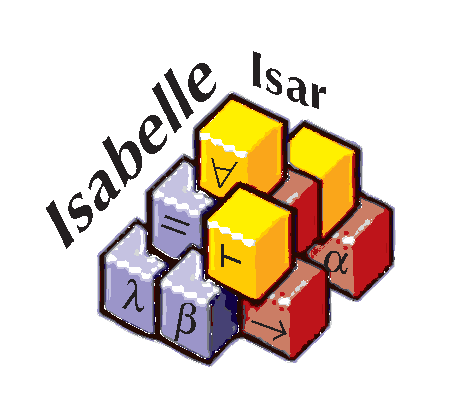
\includegraphics[scale=0.5]{isabelle_isar} \\[4ex] The Isabelle/Isar Reference Manual}
\author{\emph{Makarius Wenzel} \\[3ex]
  With Contributions by
  Clemens Ballarin,
  Stefan Berghofer, \\
  Timothy Bourke,
  Lucas Dixon,
  Florian Haftmann, \\
  Gerwin Klein,
  Alexander Krauss,
  Tobias Nipkow, \\
  David von Oheimb,
  Larry Paulson,
  and Sebastian Skalberg
}

\makeindex

\chardef\charbackquote=`\`
\newcommand{\backquote}{\mbox{\tt\charbackquote}}


\begin{document}

\maketitle 

\pagenumbering{roman} \tableofcontents \clearfirst

\part{Basic Concepts}
%
\begin{isabellebody}%
\def\isabellecontext{Introduction}%
%
\isadelimtheory
%
\endisadelimtheory
%
\isatagtheory
\isacommand{theory}\isamarkupfalse%
\ Introduction\isanewline
\isakeyword{imports}\ Setup\isanewline
\isakeyword{begin}%
\endisatagtheory
{\isafoldtheory}%
%
\isadelimtheory
%
\endisadelimtheory
%
\isamarkupchapter{Code generation from \isa{Isabelle{\isacharslash}HOL} theories%
}
\isamarkuptrue%
%
\isamarkupsection{Introduction and Overview%
}
\isamarkuptrue%
%
\begin{isamarkuptext}%
This tutorial introduces a generic code generator for the
  \isa{Isabelle} system.
  Generic in the sense that the
  \qn{target language} for which code shall ultimately be
  generated is not fixed but may be an arbitrary state-of-the-art
  functional programming language (currently, the implementation
  supports \isa{SML} \cite{SML}, \isa{OCaml} \cite{OCaml} and \isa{Haskell}
  \cite{haskell-revised-report}).

  Conceptually the code generator framework is part
  of Isabelle's \hyperlink{theory.Pure}{\mbox{\isa{Pure}}} meta logic framework; the logic
  \hyperlink{theory.HOL}{\mbox{\isa{HOL}}} which is an extension of \hyperlink{theory.Pure}{\mbox{\isa{Pure}}}
  already comes with a reasonable framework setup and thus provides
  a good working horse for raising code-generation-driven
  applications.  So, we assume some familiarity and experience
  with the ingredients of the \hyperlink{theory.HOL}{\mbox{\isa{HOL}}} distribution theories.
  (see also \cite{isa-tutorial}).

  The code generator aims to be usable with no further ado
  in most cases while allowing for detailed customisation.
  This manifests in the structure of this tutorial: after a short
  conceptual introduction with an example (\secref{sec:intro}),
  we discuss the generic customisation facilities (\secref{sec:program}).
  A further section (\secref{sec:adaption}) is dedicated to the matter of
  \qn{adaption} to specific target language environments.  After some
  further issues (\secref{sec:further}) we conclude with an overview
  of some ML programming interfaces (\secref{sec:ml}).

  \begin{warn}
    Ultimately, the code generator which this tutorial deals with
    is supposed to replace the existing code generator
    by Stefan Berghofer \cite{Berghofer-Nipkow:2002}.
    So, for the moment, there are two distinct code generators
    in Isabelle.  In case of ambiguity, we will refer to the framework
    described here as \isa{generic\ code\ generator}, to the
    other as \isa{SML\ code\ generator}.
    Also note that while the framework itself is
    object-logic independent, only \hyperlink{theory.HOL}{\mbox{\isa{HOL}}} provides a reasonable
    framework setup.    
  \end{warn}%
\end{isamarkuptext}%
\isamarkuptrue%
%
\isamarkupsubsection{Code generation via shallow embedding \label{sec:intro}%
}
\isamarkuptrue%
%
\begin{isamarkuptext}%
The key concept for understanding \isa{Isabelle}'s code generation is
  \emph{shallow embedding}, i.e.~logical entities like constants, types and
  classes are identified with corresponding concepts in the target language.

  Inside \hyperlink{theory.HOL}{\mbox{\isa{HOL}}}, the \hyperlink{command.datatype}{\mbox{\isa{\isacommand{datatype}}}} and
  \hyperlink{command.definition}{\mbox{\isa{\isacommand{definition}}}}/\hyperlink{command.primrec}{\mbox{\isa{\isacommand{primrec}}}}/\hyperlink{command.fun}{\mbox{\isa{\isacommand{fun}}}} declarations form
  the core of a functional programming language.  The default code generator setup
  allows to turn those into functional programs immediately.
  This means that \qt{naive} code generation can proceed without further ado.
  For example, here a simple \qt{implementation} of amortised queues:%
\end{isamarkuptext}%
\isamarkuptrue%
%
\isadelimquoteme
%
\endisadelimquoteme
%
\isatagquoteme
\isacommand{datatype}\isamarkupfalse%
\ {\isacharprime}a\ queue\ {\isacharequal}\ Queue\ {\isachardoublequoteopen}{\isacharprime}a\ list{\isachardoublequoteclose}\ {\isachardoublequoteopen}{\isacharprime}a\ list{\isachardoublequoteclose}\isanewline
\isanewline
\isacommand{definition}\isamarkupfalse%
\ empty\ {\isacharcolon}{\isacharcolon}\ {\isachardoublequoteopen}{\isacharprime}a\ queue{\isachardoublequoteclose}\ \isakeyword{where}\isanewline
\ \ {\isachardoublequoteopen}empty\ {\isacharequal}\ Queue\ {\isacharbrackleft}{\isacharbrackright}\ {\isacharbrackleft}{\isacharbrackright}{\isachardoublequoteclose}\isanewline
\isanewline
\isacommand{primrec}\isamarkupfalse%
\ enqueue\ {\isacharcolon}{\isacharcolon}\ {\isachardoublequoteopen}{\isacharprime}a\ {\isasymRightarrow}\ {\isacharprime}a\ queue\ {\isasymRightarrow}\ {\isacharprime}a\ queue{\isachardoublequoteclose}\ \isakeyword{where}\isanewline
\ \ {\isachardoublequoteopen}enqueue\ x\ {\isacharparenleft}Queue\ xs\ ys{\isacharparenright}\ {\isacharequal}\ Queue\ {\isacharparenleft}x\ {\isacharhash}\ xs{\isacharparenright}\ ys{\isachardoublequoteclose}\isanewline
\isanewline
\isacommand{fun}\isamarkupfalse%
\ dequeue\ {\isacharcolon}{\isacharcolon}\ {\isachardoublequoteopen}{\isacharprime}a\ queue\ {\isasymRightarrow}\ {\isacharprime}a\ option\ {\isasymtimes}\ {\isacharprime}a\ queue{\isachardoublequoteclose}\ \isakeyword{where}\isanewline
\ \ \ \ {\isachardoublequoteopen}dequeue\ {\isacharparenleft}Queue\ {\isacharbrackleft}{\isacharbrackright}\ {\isacharbrackleft}{\isacharbrackright}{\isacharparenright}\ {\isacharequal}\ {\isacharparenleft}None{\isacharcomma}\ Queue\ {\isacharbrackleft}{\isacharbrackright}\ {\isacharbrackleft}{\isacharbrackright}{\isacharparenright}{\isachardoublequoteclose}\isanewline
\ \ {\isacharbar}\ {\isachardoublequoteopen}dequeue\ {\isacharparenleft}Queue\ xs\ {\isacharparenleft}y\ {\isacharhash}\ ys{\isacharparenright}{\isacharparenright}\ {\isacharequal}\ {\isacharparenleft}Some\ y{\isacharcomma}\ Queue\ xs\ ys{\isacharparenright}{\isachardoublequoteclose}\isanewline
\ \ {\isacharbar}\ {\isachardoublequoteopen}dequeue\ {\isacharparenleft}Queue\ xs\ {\isacharbrackleft}{\isacharbrackright}{\isacharparenright}\ {\isacharequal}\isanewline
\ \ \ \ \ \ {\isacharparenleft}case\ rev\ xs\ of\ y\ {\isacharhash}\ ys\ {\isasymRightarrow}\ {\isacharparenleft}Some\ y{\isacharcomma}\ Queue\ {\isacharbrackleft}{\isacharbrackright}\ ys{\isacharparenright}{\isacharparenright}{\isachardoublequoteclose}%
\endisatagquoteme
{\isafoldquoteme}%
%
\isadelimquoteme
%
\endisadelimquoteme
%
\begin{isamarkuptext}%
\noindent Then we can generate code e.g.~for \isa{SML} as follows:%
\end{isamarkuptext}%
\isamarkuptrue%
%
\isadelimquoteme
%
\endisadelimquoteme
%
\isatagquoteme
\isacommand{export{\isacharunderscore}code}\isamarkupfalse%
\ empty\ dequeue\ enqueue\ \isakeyword{in}\ SML\isanewline
\ \ \isakeyword{module{\isacharunderscore}name}\ Example\ \isakeyword{file}\ {\isachardoublequoteopen}examples{\isacharslash}example{\isachardot}ML{\isachardoublequoteclose}%
\endisatagquoteme
{\isafoldquoteme}%
%
\isadelimquoteme
%
\endisadelimquoteme
%
\begin{isamarkuptext}%
\noindent resulting in the following code:%
\end{isamarkuptext}%
\isamarkuptrue%
%
\isadelimquoteme
%
\endisadelimquoteme
%
\isatagquoteme
%
\begin{isamarkuptext}%
\isaverbatim%
\noindent%
\verb|structure Example = |\newline%
\verb|struct|\newline%
\newline%
\verb|fun foldl f a [] = a|\newline%
\verb|  |\verb,|,\verb| foldl f a (x :: xs) = foldl f (f a x) xs;|\newline%
\newline%
\verb|fun rev xs = foldl (fn xsa => fn x => x :: xsa) [] xs;|\newline%
\newline%
\verb|fun list_case f1 f2 (a :: lista) = f2 a lista|\newline%
\verb|  |\verb,|,\verb| list_case f1 f2 [] = f1;|\newline%
\newline%
\verb|datatype 'a queue = Queue of 'a list * 'a list;|\newline%
\newline%
\verb|val empty : 'a queue = Queue ([], []);|\newline%
\newline%
\verb|fun dequeue (Queue ([], [])) = (NONE, Queue ([], []))|\newline%
\verb|  |\verb,|,\verb| dequeue (Queue (xs, y :: ys)) = (SOME y, Queue (xs, ys))|\newline%
\verb|  |\verb,|,\verb| dequeue (Queue (v :: va, [])) =|\newline%
\verb|    let|\newline%
\verb|      val y :: ys = rev (v :: va);|\newline%
\verb|    in|\newline%
\verb|      (SOME y, Queue ([], ys))|\newline%
\verb|    end;|\newline%
\newline%
\verb|fun enqueue x (Queue (xs, ys)) = Queue (x :: xs, ys);|\newline%
\newline%
\verb|end; (*struct Example*)|%
\end{isamarkuptext}%
\isamarkuptrue%
%
\endisatagquoteme
{\isafoldquoteme}%
%
\isadelimquoteme
%
\endisadelimquoteme
%
\begin{isamarkuptext}%
\noindent The \hyperlink{command.export-code}{\mbox{\isa{\isacommand{export{\isacharunderscore}code}}}} command takes a space-separated list of
  constants for which code shall be generated;  anything else needed for those
  is added implicitly.  Then follows a target language identifier
  (\isa{SML}, \isa{OCaml} or \isa{Haskell}) and a freely chosen module name.
  A file name denotes the destination to store the generated code.  Note that
  the semantics of the destination depends on the target language:  for
  \isa{SML} and \isa{OCaml} it denotes a \emph{file}, for \isa{Haskell}
  it denotes a \emph{directory} where a file named as the module name
  (with extension \isa{{\isachardot}hs}) is written:%
\end{isamarkuptext}%
\isamarkuptrue%
%
\isadelimquoteme
%
\endisadelimquoteme
%
\isatagquoteme
\isacommand{export{\isacharunderscore}code}\isamarkupfalse%
\ empty\ dequeue\ enqueue\ \isakeyword{in}\ Haskell\isanewline
\ \ \isakeyword{module{\isacharunderscore}name}\ Example\ \isakeyword{file}\ {\isachardoublequoteopen}examples{\isacharslash}{\isachardoublequoteclose}%
\endisatagquoteme
{\isafoldquoteme}%
%
\isadelimquoteme
%
\endisadelimquoteme
%
\begin{isamarkuptext}%
\noindent This is how the corresponding code in \isa{Haskell} looks like:%
\end{isamarkuptext}%
\isamarkuptrue%
%
\isadelimquoteme
%
\endisadelimquoteme
%
\isatagquoteme
%
\begin{isamarkuptext}%
\isaverbatim%
\noindent%
\verb|module Example where {|\newline%
\newline%
\newline%
\verb|foldla :: forall a b. (a -> b -> a) -> a -> [b] -> a;|\newline%
\verb|foldla f a [] = a;|\newline%
\verb|foldla f a (x : xs) = foldla f (f a x) xs;|\newline%
\newline%
\verb|rev :: forall a. [a] -> [a];|\newline%
\verb|rev xs = foldla (\ xsa x -> x : xsa) [] xs;|\newline%
\newline%
\verb|list_case :: forall t a. t -> (a -> [a] -> t) -> [a] -> t;|\newline%
\verb|list_case f1 f2 (a : list) = f2 a list;|\newline%
\verb|list_case f1 f2 [] = f1;|\newline%
\newline%
\verb|data Queue a = Queue [a] [a];|\newline%
\newline%
\verb|empty :: forall a. Queue a;|\newline%
\verb|empty = Queue [] [];|\newline%
\newline%
\verb|dequeue :: forall a. Queue a -> (Maybe a, Queue a);|\newline%
\verb|dequeue (Queue [] []) = (Nothing, Queue [] []);|\newline%
\verb|dequeue (Queue xs (y : ys)) = (Just y, Queue xs ys);|\newline%
\verb|dequeue (Queue (v : va) []) =|\newline%
\verb|  let {|\newline%
\verb|    (y : ys) = rev (v : va);|\newline%
\verb|  } in (Just y, Queue [] ys);|\newline%
\newline%
\verb|enqueue :: forall a. a -> Queue a -> Queue a;|\newline%
\verb|enqueue x (Queue xs ys) = Queue (x : xs) ys;|\newline%
\newline%
\verb|}|%
\end{isamarkuptext}%
\isamarkuptrue%
%
\endisatagquoteme
{\isafoldquoteme}%
%
\isadelimquoteme
%
\endisadelimquoteme
%
\begin{isamarkuptext}%
\noindent This demonstrates the basic usage of the \hyperlink{command.export-code}{\mbox{\isa{\isacommand{export{\isacharunderscore}code}}}} command;
  for more details see \secref{sec:further}.%
\end{isamarkuptext}%
\isamarkuptrue%
%
\isamarkupsubsection{Code generator architecture \label{sec:concept}%
}
\isamarkuptrue%
%
\begin{isamarkuptext}%
What you have seen so far should be already enough in a lot of cases.  If you
  are content with this, you can quit reading here.  Anyway, in order to customise
  and adapt the code generator, it is inevitable to gain some understanding
  how it works.

  \begin{figure}[h]
    \centering
    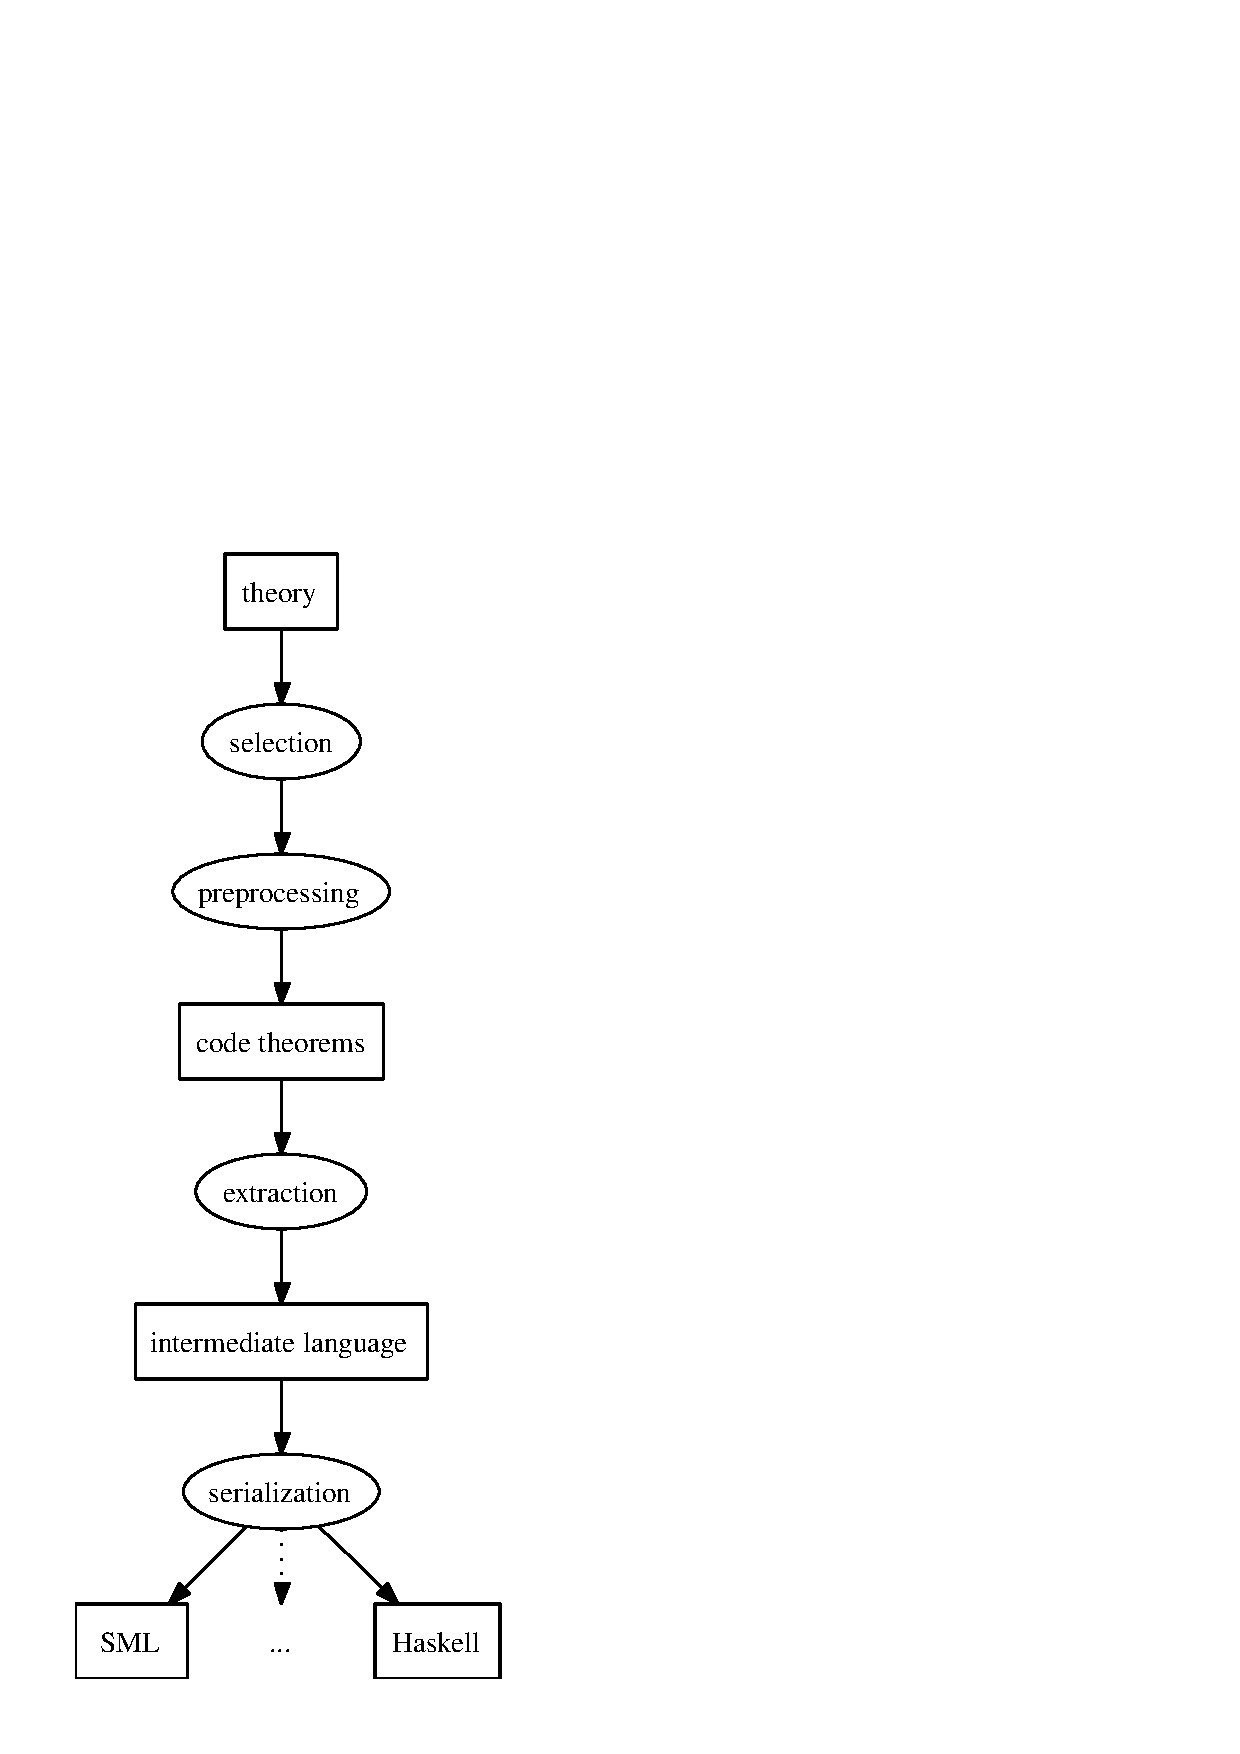
\includegraphics[width=0.7\textwidth]{codegen_process}
    \caption{Code generator architecture}
    \label{fig:arch}
  \end{figure}

  The code generator employs a notion of executability
  for three foundational executable ingredients known
  from functional programming:
  \emph{defining equations}, \emph{datatypes}, and
  \emph{type classes}.  A defining equation as a first approximation
  is a theorem of the form \isa{f\ t\isactrlisub {\isadigit{1}}\ t\isactrlisub {\isadigit{2}}\ {\isasymdots}\ t\isactrlisub n\ {\isasymequiv}\ t}
  (an equation headed by a constant \isa{f} with arguments
  \isa{t\isactrlisub {\isadigit{1}}\ t\isactrlisub {\isadigit{2}}\ {\isasymdots}\ t\isactrlisub n} and right hand side \isa{t}).
  Code generation aims to turn defining equations
  into a functional program.  This is achieved by three major
  components which operate sequentially, i.e. the result of one is
  the input
  of the next in the chain,  see diagram \ref{fig:arch}:

  \begin{itemize}

    \item Out of the vast collection of theorems proven in a
      \qn{theory}, a reasonable subset modelling
      defining equations is \qn{selected}.

    \item On those selected theorems, certain
      transformations are carried out
      (\qn{preprocessing}).  Their purpose is to turn theorems
      representing non- or badly executable
      specifications into equivalent but executable counterparts.
      The result is a structured collection of \qn{code theorems}.

    \item Before the selected defining equations are continued with,
      they can be \qn{preprocessed}, i.e. subjected to theorem
      transformations.  This \qn{preprocessor} is an interface which
      allows to apply
      the full expressiveness of ML-based theorem transformations
      to code generation;  motivating examples are shown below, see
      \secref{sec:preproc}.
      The result of the preprocessing step is a structured collection
      of defining equations.

    \item These defining equations are \qn{translated} to a program
      in an abstract intermediate language.  Think of it as a kind
      of \qt{Mini-Haskell} with four \qn{statements}: \isa{data}
      (for datatypes), \isa{fun} (stemming from defining equations),
      also \isa{class} and \isa{inst} (for type classes).

    \item Finally, the abstract program is \qn{serialised} into concrete
      source code of a target language.

  \end{itemize}

  \noindent From these steps, only the two last are carried out outside the logic;  by
  keeping this layer as thin as possible, the amount of code to trust is
  kept to a minimum.%
\end{isamarkuptext}%
\isamarkuptrue%
%
\isadelimtheory
%
\endisadelimtheory
%
\isatagtheory
\isacommand{end}\isamarkupfalse%
%
\endisatagtheory
{\isafoldtheory}%
%
\isadelimtheory
%
\endisadelimtheory
\isanewline
\end{isabellebody}%
%%% Local Variables:
%%% mode: latex
%%% TeX-master: "root"
%%% End:

%
\begin{isabellebody}%
\def\isabellecontext{Framework}%
%
\isadelimtheory
%
\endisadelimtheory
%
\isatagtheory
\isacommand{theory}\isamarkupfalse%
\ Framework\isanewline
\isakeyword{imports}\ Main\isanewline
\isakeyword{begin}%
\endisatagtheory
{\isafoldtheory}%
%
\isadelimtheory
%
\endisadelimtheory
%
\isamarkupchapter{The Isabelle/Isar Framework \label{ch:isar-framework}%
}
\isamarkuptrue%
%
\begin{isamarkuptext}%
Isabelle/Isar
  \cite{Wenzel:1999:TPHOL,Wenzel-PhD,Nipkow-TYPES02,Wenzel-Paulson:2006,Wenzel:2006:Festschrift}
  is intended as a generic framework for developing formal
  mathematical documents with full proof checking.  Definitions and
  proofs are organized as theories; an assembly of theory sources may
  be presented as a printed document; see also
  \chref{ch:document-prep}.

  The main objective of Isar is the design of a human-readable
  structured proof language, which is called the ``primary proof
  format'' in Isar terminology.  Such a primary proof language is
  somewhere in the middle between the extremes of primitive proof
  objects and actual natural language.  In this respect, Isar is a bit
  more formalistic than Mizar
  \cite{Trybulec:1993:MizarFeatures,Rudnicki:1992:MizarOverview,Wiedijk:1999:Mizar},
  using logical symbols for certain reasoning schemes where Mizar
  would prefer English words; see \cite{Wenzel-Wiedijk:2002} for
  further comparisons of these systems.

  So Isar challenges the traditional way of recording informal proofs
  in mathematical prose, as well as the common tendency to see fully
  formal proofs directly as objects of some logical calculus (e.g.\
  \isa{{\isachardoublequote}{\isasymlambda}{\isachardoublequote}}-terms in a version of type theory).  In fact, Isar is
  better understood as an interpreter of a simple block-structured
  language for describing data flow of local facts and goals,
  interspersed with occasional invocations of proof methods.
  Everything is reduced to logical inferences internally, but these
  steps are somewhat marginal compared to the overall bookkeeping of
  the interpretation process.  Thanks to careful design of the syntax
  and semantics of Isar language elements, a formal record of Isar
  instructions may later appear as an intelligible text to the
  attentive reader.

  The Isar proof language has emerged from careful analysis of some
  inherent virtues of the existing logical framework of Isabelle/Pure
  \cite{paulson-found,paulson700}, notably composition of higher-order
  natural deduction rules, which is a generalization of Gentzen's
  original calculus \cite{Gentzen:1935}.  The approach of generic
  inference systems in Pure is continued by Isar towards actual proof
  texts.

  Concrete applications require another intermediate layer: an
  object-logic.  Isabelle/HOL \cite{isa-tutorial} (simply-typed
  set-theory) is being used most of the time; Isabelle/ZF
  \cite{isabelle-ZF} is less extensively developed, although it would
  probably fit better for classical mathematics.

  \medskip In order to illustrate typical natural deduction reasoning
  in Isar, we shall refer to the background theory and library of
  Isabelle/HOL.  This includes common notions of predicate logic,
  naive set-theory etc.\ using fairly standard mathematical notation.
  From the perspective of generic natural deduction there is nothing
  special about the logical connectives of HOL (\isa{{\isachardoublequote}{\isasymand}{\isachardoublequote}}, \isa{{\isachardoublequote}{\isasymor}{\isachardoublequote}}, \isa{{\isachardoublequote}{\isasymforall}{\isachardoublequote}}, \isa{{\isachardoublequote}{\isasymexists}{\isachardoublequote}}, etc.), only the resulting reasoning
  principles are relevant to the user.  There are similar rules
  available for set-theory operators (\isa{{\isachardoublequote}{\isasyminter}{\isachardoublequote}}, \isa{{\isachardoublequote}{\isasymunion}{\isachardoublequote}}, \isa{{\isachardoublequote}{\isasymInter}{\isachardoublequote}}, \isa{{\isachardoublequote}{\isasymUnion}{\isachardoublequote}}, etc.), or any other theory developed in the
  library (lattice theory, topology etc.).

  Subsequently we briefly review fragments of Isar proof texts
  corresponding directly to such general natural deduction schemes.
  The examples shall refer to set-theory, to minimize the danger of
  understanding connectives of predicate logic as something special.

  \medskip The following deduction performs \isa{{\isachardoublequote}{\isasyminter}{\isachardoublequote}}-introduction,
  working forwards from assumptions towards the conclusion.  We give
  both the Isar text, and depict the primitive rule involved, as
  determined by unification of the problem against rules from the
  context.%
\end{isamarkuptext}%
\isamarkuptrue%
%
\medskip\begin{minipage}{0.6\textwidth}
%
\isadelimproof
%
\endisadelimproof
%
\isatagproof
\ \ \ \ \isacommand{assume}\isamarkupfalse%
\ {\isachardoublequoteopen}x\ {\isasymin}\ A{\isachardoublequoteclose}\ \isakeyword{and}\ {\isachardoublequoteopen}x\ {\isasymin}\ B{\isachardoublequoteclose}\isanewline
\ \ \ \ \isacommand{then}\isamarkupfalse%
\ \isacommand{have}\isamarkupfalse%
\ {\isachardoublequoteopen}x\ {\isasymin}\ A\ {\isasyminter}\ B{\isachardoublequoteclose}\ \isacommand{{\isachardot}{\isachardot}}\isamarkupfalse%
%
\endisatagproof
{\isafoldproof}%
%
\isadelimproof
%
\endisadelimproof
%
\end{minipage}\begin{minipage}{0.4\textwidth}
%
\begin{isamarkuptext}%
\infer{\isa{{\isachardoublequote}x\ {\isasymin}\ A\ {\isasyminter}\ B{\isachardoublequote}}}{\isa{{\isachardoublequote}x\ {\isasymin}\ A{\isachardoublequote}} & \isa{{\isachardoublequote}x\ {\isasymin}\ B{\isachardoublequote}}}%
\end{isamarkuptext}%
\isamarkuptrue%
%
\end{minipage}
%
\begin{isamarkuptext}%
\medskip\noindent Note that \hyperlink{command.assume}{\mbox{\isa{\isacommand{assume}}}} augments the
  context, \hyperlink{command.then}{\mbox{\isa{\isacommand{then}}}} indicates that the current facts shall be
  used in the next step, and \hyperlink{command.have}{\mbox{\isa{\isacommand{have}}}} states a local claim.
  The two dots ``\hyperlink{command.ddot}{\mbox{\isa{\isacommand{{\isachardot}{\isachardot}}}}}'' above refer to a complete proof of
  the claim, using the indicated facts and a canonical rule from the
  context.  We could have been more explicit here by spelling out the
  final proof step via the \hyperlink{command.by}{\mbox{\isa{\isacommand{by}}}} command:%
\end{isamarkuptext}%
\isamarkuptrue%
%
\isadelimproof
%
\endisadelimproof
%
\isatagproof
\ \ \ \ \isacommand{assume}\isamarkupfalse%
\ {\isachardoublequoteopen}x\ {\isasymin}\ A{\isachardoublequoteclose}\ \isakeyword{and}\ {\isachardoublequoteopen}x\ {\isasymin}\ B{\isachardoublequoteclose}\isanewline
\ \ \ \ \isacommand{then}\isamarkupfalse%
\ \isacommand{have}\isamarkupfalse%
\ {\isachardoublequoteopen}x\ {\isasymin}\ A\ {\isasyminter}\ B{\isachardoublequoteclose}\ \isacommand{by}\isamarkupfalse%
\ {\isacharparenleft}rule\ IntI{\isacharparenright}%
\endisatagproof
{\isafoldproof}%
%
\isadelimproof
%
\endisadelimproof
%
\begin{isamarkuptext}%
\noindent The format of the \isa{{\isachardoublequote}{\isasyminter}{\isachardoublequote}}-introduction rule represents
  the most basic inference, which proceeds from given premises to a
  conclusion, without any additional context involved.

  \medskip The next example performs backwards introduction on \isa{{\isachardoublequote}{\isasymInter}{\isasymA}{\isachardoublequote}}, the intersection of all sets within a given set.  This
  requires a nested proof of set membership within a local context of
  an arbitrary-but-fixed member of the collection:%
\end{isamarkuptext}%
\isamarkuptrue%
%
\medskip\begin{minipage}{0.6\textwidth}
%
\isadelimproof
%
\endisadelimproof
%
\isatagproof
\ \ \ \ \isacommand{have}\isamarkupfalse%
\ {\isachardoublequoteopen}x\ {\isasymin}\ {\isasymInter}{\isasymA}{\isachardoublequoteclose}\isanewline
\ \ \ \ \isacommand{proof}\isamarkupfalse%
\isanewline
\ \ \ \ \ \ \isacommand{fix}\isamarkupfalse%
\ A\isanewline
\ \ \ \ \ \ \isacommand{assume}\isamarkupfalse%
\ {\isachardoublequoteopen}A\ {\isasymin}\ {\isasymA}{\isachardoublequoteclose}\isanewline
\ \ \ \ \ \ \isacommand{show}\isamarkupfalse%
\ {\isachardoublequoteopen}x\ {\isasymin}\ A{\isachardoublequoteclose}\ \isacommand{sorry}\isamarkupfalse%
\isanewline
\ \ \ \ \isacommand{qed}\isamarkupfalse%
%
\endisatagproof
{\isafoldproof}%
%
\isadelimproof
%
\endisadelimproof
%
\end{minipage}\begin{minipage}{0.4\textwidth}
%
\begin{isamarkuptext}%
\infer{\isa{{\isachardoublequote}x\ {\isasymin}\ {\isasymInter}{\isasymA}{\isachardoublequote}}}{\infer*{\isa{{\isachardoublequote}x\ {\isasymin}\ A{\isachardoublequote}}}{\isa{{\isachardoublequote}{\isacharbrackleft}A{\isacharbrackright}{\isacharbrackleft}A\ {\isasymin}\ {\isasymA}{\isacharbrackright}{\isachardoublequote}}}}%
\end{isamarkuptext}%
\isamarkuptrue%
%
\end{minipage}
%
\begin{isamarkuptext}%
\medskip\noindent This Isar reasoning pattern again refers to the
  primitive rule depicted above.  The system determines it in the
  ``\hyperlink{command.proof}{\mbox{\isa{\isacommand{proof}}}}'' step, which could have been spelt out more
  explicitly as ``\hyperlink{command.proof}{\mbox{\isa{\isacommand{proof}}}}~\isa{{\isachardoublequote}{\isacharparenleft}rule\ InterI{\isacharparenright}{\isachardoublequote}}''.  Note
  that this rule involves both a local parameter \isa{{\isachardoublequote}A{\isachardoublequote}} and an
  assumption \isa{{\isachardoublequote}A\ {\isasymin}\ {\isasymA}{\isachardoublequote}} in the nested reasoning.  This kind of
  compound rule typically demands a genuine sub-proof in Isar, working
  backwards rather than forwards as seen before.  In the proof body we
  encounter the \hyperlink{command.fix}{\mbox{\isa{\isacommand{fix}}}}-\hyperlink{command.assume}{\mbox{\isa{\isacommand{assume}}}}-\hyperlink{command.show}{\mbox{\isa{\isacommand{show}}}}
  skeleton of nested sub-proofs that is typical for Isar.  The final
  \hyperlink{command.show}{\mbox{\isa{\isacommand{show}}}} is like \hyperlink{command.have}{\mbox{\isa{\isacommand{have}}}} followed by an
  additional refinement of the enclosing claim, using the rule derived
  from the proof body.  The \hyperlink{command.sorry}{\mbox{\isa{\isacommand{sorry}}}} command stands for a
  hole in the proof --- it may be understood as an excuse for not
  providing a proper proof yet.

  \medskip The next example involves \isa{{\isachardoublequote}{\isasymUnion}{\isasymA}{\isachardoublequote}}, which can be
  characterized as the set of all \isa{{\isachardoublequote}x{\isachardoublequote}} such that \isa{{\isachardoublequote}{\isasymexists}A{\isachardot}\ x\ {\isasymin}\ A\ {\isasymand}\ A\ {\isasymin}\ {\isasymA}{\isachardoublequote}}.  The elimination rule for \isa{{\isachardoublequote}x\ {\isasymin}\ {\isasymUnion}{\isasymA}{\isachardoublequote}} does
  not mention \isa{{\isachardoublequote}{\isasymexists}{\isachardoublequote}} and \isa{{\isachardoublequote}{\isasymand}{\isachardoublequote}} at all, but admits to obtain
  directly a local \isa{{\isachardoublequote}A{\isachardoublequote}} such that \isa{{\isachardoublequote}x\ {\isasymin}\ A{\isachardoublequote}} and \isa{{\isachardoublequote}A\ {\isasymin}\ {\isasymA}{\isachardoublequote}} hold.  This corresponds to the following Isar proof and
  inference rule, respectively:%
\end{isamarkuptext}%
\isamarkuptrue%
%
\medskip\begin{minipage}{0.6\textwidth}
%
\isadelimproof
%
\endisadelimproof
%
\isatagproof
\ \ \ \ \isacommand{assume}\isamarkupfalse%
\ {\isachardoublequoteopen}x\ {\isasymin}\ {\isasymUnion}{\isasymA}{\isachardoublequoteclose}\isanewline
\ \ \ \ \isacommand{then}\isamarkupfalse%
\ \isacommand{have}\isamarkupfalse%
\ C\isanewline
\ \ \ \ \isacommand{proof}\isamarkupfalse%
\isanewline
\ \ \ \ \ \ \isacommand{fix}\isamarkupfalse%
\ A\isanewline
\ \ \ \ \ \ \isacommand{assume}\isamarkupfalse%
\ {\isachardoublequoteopen}x\ {\isasymin}\ A{\isachardoublequoteclose}\ \isakeyword{and}\ {\isachardoublequoteopen}A\ {\isasymin}\ {\isasymA}{\isachardoublequoteclose}\isanewline
\ \ \ \ \ \ \isacommand{show}\isamarkupfalse%
\ C\ \isacommand{sorry}\isamarkupfalse%
\isanewline
\ \ \ \ \isacommand{qed}\isamarkupfalse%
%
\endisatagproof
{\isafoldproof}%
%
\isadelimproof
%
\endisadelimproof
%
\end{minipage}\begin{minipage}{0.4\textwidth}
%
\begin{isamarkuptext}%
\infer{\isa{{\isachardoublequote}C{\isachardoublequote}}}{\isa{{\isachardoublequote}x\ {\isasymin}\ {\isasymUnion}{\isasymA}{\isachardoublequote}} & \infer*{\isa{{\isachardoublequote}C{\isachardoublequote}}~}{\isa{{\isachardoublequote}{\isacharbrackleft}A{\isacharbrackright}{\isacharbrackleft}x\ {\isasymin}\ A{\isacharcomma}\ A\ {\isasymin}\ {\isasymA}{\isacharbrackright}{\isachardoublequote}}}}%
\end{isamarkuptext}%
\isamarkuptrue%
%
\end{minipage}
%
\begin{isamarkuptext}%
\medskip\noindent Although the Isar proof follows the natural
  deduction rule closely, the text reads not as natural as
  anticipated.  There is a double occurrence of an arbitrary
  conclusion \isa{{\isachardoublequote}C{\isachardoublequote}}, which represents the final result, but is
  irrelevant for now.  This issue arises for any elimination rule
  involving local parameters.  Isar provides the derived language
  element \hyperlink{command.obtain}{\mbox{\isa{\isacommand{obtain}}}}, which is able to perform the same
  elimination proof more conveniently:%
\end{isamarkuptext}%
\isamarkuptrue%
%
\isadelimproof
%
\endisadelimproof
%
\isatagproof
\ \ \ \ \isacommand{assume}\isamarkupfalse%
\ {\isachardoublequoteopen}x\ {\isasymin}\ {\isasymUnion}{\isasymA}{\isachardoublequoteclose}\isanewline
\ \ \ \ \isacommand{then}\isamarkupfalse%
\ \isacommand{obtain}\isamarkupfalse%
\ A\ \isakeyword{where}\ {\isachardoublequoteopen}x\ {\isasymin}\ A{\isachardoublequoteclose}\ \isakeyword{and}\ {\isachardoublequoteopen}A\ {\isasymin}\ {\isasymA}{\isachardoublequoteclose}\ \isacommand{{\isachardot}{\isachardot}}\isamarkupfalse%
%
\endisatagproof
{\isafoldproof}%
%
\isadelimproof
%
\endisadelimproof
%
\begin{isamarkuptext}%
\noindent Here we avoid to mention the final conclusion \isa{{\isachardoublequote}C{\isachardoublequote}}
  and return to plain forward reasoning.  The rule involved in the
  ``\hyperlink{command.ddot}{\mbox{\isa{\isacommand{{\isachardot}{\isachardot}}}}}'' proof is the same as before.%
\end{isamarkuptext}%
\isamarkuptrue%
%
\isamarkupsection{The Pure framework \label{sec:framework-pure}%
}
\isamarkuptrue%
%
\begin{isamarkuptext}%
The Pure logic \cite{paulson-found,paulson700} is an intuitionistic
  fragment of higher-order logic \cite{church40}.  In type-theoretic
  parlance, there are three levels of \isa{{\isachardoublequote}{\isasymlambda}{\isachardoublequote}}-calculus with
  corresponding arrows: \isa{{\isachardoublequote}{\isasymRightarrow}{\isachardoublequote}} for syntactic function space
  (terms depending on terms), \isa{{\isachardoublequote}{\isasymAnd}{\isachardoublequote}} for universal quantification
  (proofs depending on terms), and \isa{{\isachardoublequote}{\isasymLongrightarrow}{\isachardoublequote}} for implication (proofs
  depending on proofs).

  On top of this, Pure implements a generic calculus for nested
  natural deduction rules, similar to \cite{Schroeder-Heister:1984}.
  Here object-logic inferences are internalized as formulae over
  \isa{{\isachardoublequote}{\isasymAnd}{\isachardoublequote}} and \isa{{\isachardoublequote}{\isasymLongrightarrow}{\isachardoublequote}}.  Combining such rule statements may
  involve higher-order unification \cite{paulson-natural}.%
\end{isamarkuptext}%
\isamarkuptrue%
%
\isamarkupsubsection{Primitive inferences%
}
\isamarkuptrue%
%
\begin{isamarkuptext}%
Term syntax provides explicit notation for abstraction \isa{{\isachardoublequote}{\isasymlambda}x\ {\isacharcolon}{\isacharcolon}\ {\isasymalpha}{\isachardot}\ b{\isacharparenleft}x{\isacharparenright}{\isachardoublequote}} and application \isa{{\isachardoublequote}b\ a{\isachardoublequote}}, while types are usually
  implicit thanks to type-inference; terms of type \isa{{\isachardoublequote}prop{\isachardoublequote}} are
  called propositions.  Logical statements are composed via \isa{{\isachardoublequote}{\isasymAnd}x\ {\isacharcolon}{\isacharcolon}\ {\isasymalpha}{\isachardot}\ B{\isacharparenleft}x{\isacharparenright}{\isachardoublequote}} and \isa{{\isachardoublequote}A\ {\isasymLongrightarrow}\ B{\isachardoublequote}}.  Primitive reasoning operates on
  judgments of the form \isa{{\isachardoublequote}{\isasymGamma}\ {\isasymturnstile}\ {\isasymphi}{\isachardoublequote}}, with standard introduction
  and elimination rules for \isa{{\isachardoublequote}{\isasymAnd}{\isachardoublequote}} and \isa{{\isachardoublequote}{\isasymLongrightarrow}{\isachardoublequote}} that refer to
  fixed parameters \isa{{\isachardoublequote}x\isactrlisub {\isadigit{1}}{\isacharcomma}\ {\isasymdots}{\isacharcomma}\ x\isactrlisub m{\isachardoublequote}} and hypotheses
  \isa{{\isachardoublequote}A\isactrlisub {\isadigit{1}}{\isacharcomma}\ {\isasymdots}{\isacharcomma}\ A\isactrlisub n{\isachardoublequote}} from the context \isa{{\isachardoublequote}{\isasymGamma}{\isachardoublequote}};
  the corresponding proof terms are left implicit.  The subsequent
  inference rules define \isa{{\isachardoublequote}{\isasymGamma}\ {\isasymturnstile}\ {\isasymphi}{\isachardoublequote}} inductively, relative to a
  collection of axioms:

  \[
  \infer{\isa{{\isachardoublequote}{\isasymturnstile}\ A{\isachardoublequote}}}{(\isa{{\isachardoublequote}A{\isachardoublequote}} \text{~axiom})}
  \qquad
  \infer{\isa{{\isachardoublequote}A\ {\isasymturnstile}\ A{\isachardoublequote}}}{}
  \]

  \[
  \infer{\isa{{\isachardoublequote}{\isasymGamma}\ {\isasymturnstile}\ {\isasymAnd}x{\isachardot}\ B{\isacharparenleft}x{\isacharparenright}{\isachardoublequote}}}{\isa{{\isachardoublequote}{\isasymGamma}\ {\isasymturnstile}\ B{\isacharparenleft}x{\isacharparenright}{\isachardoublequote}} & \isa{{\isachardoublequote}x\ {\isasymnotin}\ {\isasymGamma}{\isachardoublequote}}}
  \qquad
  \infer{\isa{{\isachardoublequote}{\isasymGamma}\ {\isasymturnstile}\ B{\isacharparenleft}a{\isacharparenright}{\isachardoublequote}}}{\isa{{\isachardoublequote}{\isasymGamma}\ {\isasymturnstile}\ {\isasymAnd}x{\isachardot}\ B{\isacharparenleft}x{\isacharparenright}{\isachardoublequote}}}
  \]

  \[
  \infer{\isa{{\isachardoublequote}{\isasymGamma}\ {\isacharminus}\ A\ {\isasymturnstile}\ A\ {\isasymLongrightarrow}\ B{\isachardoublequote}}}{\isa{{\isachardoublequote}{\isasymGamma}\ {\isasymturnstile}\ B{\isachardoublequote}}}
  \qquad
  \infer{\isa{{\isachardoublequote}{\isasymGamma}\isactrlsub {\isadigit{1}}\ {\isasymunion}\ {\isasymGamma}\isactrlsub {\isadigit{2}}\ {\isasymturnstile}\ B{\isachardoublequote}}}{\isa{{\isachardoublequote}{\isasymGamma}\isactrlsub {\isadigit{1}}\ {\isasymturnstile}\ A\ {\isasymLongrightarrow}\ B{\isachardoublequote}} & \isa{{\isachardoublequote}{\isasymGamma}\isactrlsub {\isadigit{2}}\ {\isasymturnstile}\ A{\isachardoublequote}}}
  \]

  Furthermore, Pure provides a built-in equality \isa{{\isachardoublequote}{\isasymequiv}\ {\isacharcolon}{\isacharcolon}\ {\isasymalpha}\ {\isasymRightarrow}\ {\isasymalpha}\ {\isasymRightarrow}\ prop{\isachardoublequote}} with axioms for reflexivity, substitution, extensionality,
  and \isa{{\isachardoublequote}{\isasymalpha}{\isasymbeta}{\isasymeta}{\isachardoublequote}}-conversion on \isa{{\isachardoublequote}{\isasymlambda}{\isachardoublequote}}-terms.

  \medskip An object-logic introduces another layer on top of Pure,
  e.g.\ with types \isa{{\isachardoublequote}i{\isachardoublequote}} for individuals and \isa{{\isachardoublequote}o{\isachardoublequote}} for
  propositions, term constants \isa{{\isachardoublequote}Trueprop\ {\isacharcolon}{\isacharcolon}\ o\ {\isasymRightarrow}\ prop{\isachardoublequote}} as
  (implicit) derivability judgment and connectives like \isa{{\isachardoublequote}{\isasymand}\ {\isacharcolon}{\isacharcolon}\ o\ {\isasymRightarrow}\ o\ {\isasymRightarrow}\ o{\isachardoublequote}} or \isa{{\isachardoublequote}{\isasymforall}\ {\isacharcolon}{\isacharcolon}\ {\isacharparenleft}i\ {\isasymRightarrow}\ o{\isacharparenright}\ {\isasymRightarrow}\ o{\isachardoublequote}}, and axioms for object-level
  rules such as \isa{{\isachardoublequote}conjI{\isacharcolon}\ A\ {\isasymLongrightarrow}\ B\ {\isasymLongrightarrow}\ A\ {\isasymand}\ B{\isachardoublequote}} or \isa{{\isachardoublequote}allI{\isacharcolon}\ {\isacharparenleft}{\isasymAnd}x{\isachardot}\ B\ x{\isacharparenright}\ {\isasymLongrightarrow}\ {\isasymforall}x{\isachardot}\ B\ x{\isachardoublequote}}.  Derived object rules are represented as theorems of
  Pure.  After the initial object-logic setup, further axiomatizations
  are usually avoided; plain definitions and derived principles are
  used exclusively.%
\end{isamarkuptext}%
\isamarkuptrue%
%
\isamarkupsubsection{Reasoning with rules \label{sec:framework-resolution}%
}
\isamarkuptrue%
%
\begin{isamarkuptext}%
Primitive inferences mostly serve foundational purposes.  The main
  reasoning mechanisms of Pure operate on nested natural deduction
  rules expressed as formulae, using \isa{{\isachardoublequote}{\isasymAnd}{\isachardoublequote}} to bind local
  parameters and \isa{{\isachardoublequote}{\isasymLongrightarrow}{\isachardoublequote}} to express entailment.  Multiple
  parameters and premises are represented by repeating these
  connectives in a right-associative fashion.

  Since \isa{{\isachardoublequote}{\isasymAnd}{\isachardoublequote}} and \isa{{\isachardoublequote}{\isasymLongrightarrow}{\isachardoublequote}} commute thanks to the theorem
  \isa{{\isachardoublequote}{\isacharparenleft}A\ {\isasymLongrightarrow}\ {\isacharparenleft}{\isasymAnd}x{\isachardot}\ B\ x{\isacharparenright}{\isacharparenright}\ {\isasymequiv}\ {\isacharparenleft}{\isasymAnd}x{\isachardot}\ A\ {\isasymLongrightarrow}\ B\ x{\isacharparenright}{\isachardoublequote}}, we may assume w.l.o.g.\
  that rule statements always observe the normal form where
  quantifiers are pulled in front of implications at each level of
  nesting.  This means that any Pure proposition may be presented as a
  \emph{Hereditary Harrop Formula} \cite{Miller:1991} which is of the
  form \isa{{\isachardoublequote}{\isasymAnd}x\isactrlisub {\isadigit{1}}\ {\isasymdots}\ x\isactrlisub m{\isachardot}\ H\isactrlisub {\isadigit{1}}\ {\isasymLongrightarrow}\ {\isasymdots}\ H\isactrlisub n\ {\isasymLongrightarrow}\ A{\isachardoublequote}} for \isa{{\isachardoublequote}m{\isacharcomma}\ n\ {\isasymge}\ {\isadigit{0}}{\isachardoublequote}}, and \isa{{\isachardoublequote}H\isactrlisub {\isadigit{1}}{\isacharcomma}\ {\isasymdots}{\isacharcomma}\ H\isactrlisub n{\isachardoublequote}}
  being recursively of the same format, and \isa{{\isachardoublequote}A{\isachardoublequote}} atomic.
  Following the convention that outermost quantifiers are implicit,
  Horn clauses \isa{{\isachardoublequote}A\isactrlisub {\isadigit{1}}\ {\isasymLongrightarrow}\ {\isasymdots}\ A\isactrlisub n\ {\isasymLongrightarrow}\ A{\isachardoublequote}} are a special
  case of this.

  \medskip Goals are also represented as rules: \isa{{\isachardoublequote}A\isactrlisub {\isadigit{1}}\ {\isasymLongrightarrow}\ {\isasymdots}\ A\isactrlisub n\ {\isasymLongrightarrow}\ C{\isachardoublequote}} states that the sub-goals \isa{{\isachardoublequote}A\isactrlisub {\isadigit{1}}{\isacharcomma}\ {\isasymdots}{\isacharcomma}\ A\isactrlisub n{\isachardoublequote}} entail the result \isa{{\isachardoublequote}C{\isachardoublequote}}; for \isa{{\isachardoublequote}n\ {\isacharequal}\ {\isadigit{0}}{\isachardoublequote}} the
  goal is finished.  To allow \isa{{\isachardoublequote}C{\isachardoublequote}} being a rule statement
  itself, we introduce the protective marker \isa{{\isachardoublequote}{\isacharhash}\ {\isacharcolon}{\isacharcolon}\ prop\ {\isasymRightarrow}\ prop{\isachardoublequote}}, which is defined as identity and hidden from the user.  We
  initialize and finish goal states as follows:

  \[
  \begin{array}{c@ {\qquad}c}
  \infer[(\indexdef{}{inference}{init}\hypertarget{inference.init}{\hyperlink{inference.init}{\mbox{\isa{init}}}})]{\isa{{\isachardoublequote}C\ {\isasymLongrightarrow}\ {\isacharhash}C{\isachardoublequote}}}{} &
  \infer[(\indexdef{}{inference}{finish}\hypertarget{inference.finish}{\hyperlink{inference.finish}{\mbox{\isa{finish}}}})]{\isa{C}}{\isa{{\isachardoublequote}{\isacharhash}C{\isachardoublequote}}}
  \end{array}
  \]

  Goal states are refined in intermediate proof steps until a finished
  form is achieved.  Here the two main reasoning principles are
  \hyperlink{inference.resolution}{\mbox{\isa{resolution}}}, for back-chaining a rule against a sub-goal
  (replacing it by zero or more sub-goals), and \hyperlink{inference.assumption}{\mbox{\isa{assumption}}}, for solving a sub-goal (finding a short-circuit with
  local assumptions).  Below \isa{{\isachardoublequote}\isactrlvec x{\isachardoublequote}} stands for \isa{{\isachardoublequote}x\isactrlisub {\isadigit{1}}{\isacharcomma}\ {\isasymdots}{\isacharcomma}\ x\isactrlisub n{\isachardoublequote}} (\isa{{\isachardoublequote}n\ {\isasymge}\ {\isadigit{0}}{\isachardoublequote}}).

  \[
  \infer[(\indexdef{}{inference}{resolution}\hypertarget{inference.resolution}{\hyperlink{inference.resolution}{\mbox{\isa{resolution}}}})]
  {\isa{{\isachardoublequote}{\isacharparenleft}{\isasymAnd}\isactrlvec x{\isachardot}\ \isactrlvec H\ \isactrlvec x\ {\isasymLongrightarrow}\ \isactrlvec A\ {\isacharparenleft}\isactrlvec a\ \isactrlvec x{\isacharparenright}{\isacharparenright}{\isasymvartheta}\ {\isasymLongrightarrow}\ C{\isasymvartheta}{\isachardoublequote}}}
  {\begin{tabular}{rl}
    \isa{{\isachardoublequote}rule{\isacharcolon}{\isachardoublequote}} &
    \isa{{\isachardoublequote}\isactrlvec A\ \isactrlvec a\ {\isasymLongrightarrow}\ B\ \isactrlvec a{\isachardoublequote}} \\
    \isa{{\isachardoublequote}goal{\isacharcolon}{\isachardoublequote}} &
    \isa{{\isachardoublequote}{\isacharparenleft}{\isasymAnd}\isactrlvec x{\isachardot}\ \isactrlvec H\ \isactrlvec x\ {\isasymLongrightarrow}\ B{\isacharprime}\ \isactrlvec x{\isacharparenright}\ {\isasymLongrightarrow}\ C{\isachardoublequote}} \\
    \isa{{\isachardoublequote}goal\ unifier{\isacharcolon}{\isachardoublequote}} &
    \isa{{\isachardoublequote}{\isacharparenleft}{\isasymlambda}\isactrlvec x{\isachardot}\ B\ {\isacharparenleft}\isactrlvec a\ \isactrlvec x{\isacharparenright}{\isacharparenright}{\isasymvartheta}\ {\isacharequal}\ B{\isacharprime}{\isasymvartheta}{\isachardoublequote}} \\
   \end{tabular}}
  \]

  \medskip

  \[
  \infer[(\indexdef{}{inference}{assumption}\hypertarget{inference.assumption}{\hyperlink{inference.assumption}{\mbox{\isa{assumption}}}})]{\isa{{\isachardoublequote}C{\isasymvartheta}{\isachardoublequote}}}
  {\begin{tabular}{rl}
    \isa{{\isachardoublequote}goal{\isacharcolon}{\isachardoublequote}} &
    \isa{{\isachardoublequote}{\isacharparenleft}{\isasymAnd}\isactrlvec x{\isachardot}\ \isactrlvec H\ \isactrlvec x\ {\isasymLongrightarrow}\ A\ \isactrlvec x{\isacharparenright}\ {\isasymLongrightarrow}\ C{\isachardoublequote}} \\
    \isa{{\isachardoublequote}assm\ unifier{\isacharcolon}{\isachardoublequote}} & \isa{{\isachardoublequote}A{\isasymvartheta}\ {\isacharequal}\ H\isactrlsub i{\isasymvartheta}{\isachardoublequote}}~~\text{(for some~\isa{{\isachardoublequote}H\isactrlsub i{\isachardoublequote}})} \\
   \end{tabular}}
  \]

  The following trace illustrates goal-oriented reasoning in
  Isabelle/Pure:

  \medskip
  \begin{tabular}{r@ {\qquad}l}
  \isa{{\isachardoublequote}{\isacharparenleft}A\ {\isasymand}\ B\ {\isasymLongrightarrow}\ B\ {\isasymand}\ A{\isacharparenright}\ {\isasymLongrightarrow}\ {\isacharhash}{\isacharparenleft}A\ {\isasymand}\ B\ {\isasymLongrightarrow}\ B\ {\isasymand}\ A{\isacharparenright}{\isachardoublequote}} & \isa{{\isachardoublequote}{\isacharparenleft}init{\isacharparenright}{\isachardoublequote}} \\
  \isa{{\isachardoublequote}{\isacharparenleft}A\ {\isasymand}\ B\ {\isasymLongrightarrow}\ B{\isacharparenright}\ {\isasymLongrightarrow}\ {\isacharparenleft}A\ {\isasymand}\ B\ {\isasymLongrightarrow}\ A{\isacharparenright}\ {\isasymLongrightarrow}\ {\isacharhash}{\isasymdots}{\isachardoublequote}} & \isa{{\isachardoublequote}{\isacharparenleft}resolution\ B\ {\isasymLongrightarrow}\ A\ {\isasymLongrightarrow}\ B\ {\isasymand}\ A{\isacharparenright}{\isachardoublequote}} \\
  \isa{{\isachardoublequote}{\isacharparenleft}A\ {\isasymand}\ B\ {\isasymLongrightarrow}\ A\ {\isasymand}\ B{\isacharparenright}\ {\isasymLongrightarrow}\ {\isacharparenleft}A\ {\isasymand}\ B\ {\isasymLongrightarrow}\ A{\isacharparenright}\ {\isasymLongrightarrow}\ {\isacharhash}{\isasymdots}{\isachardoublequote}} & \isa{{\isachardoublequote}{\isacharparenleft}resolution\ A\ {\isasymand}\ B\ {\isasymLongrightarrow}\ B{\isacharparenright}{\isachardoublequote}} \\
  \isa{{\isachardoublequote}{\isacharparenleft}A\ {\isasymand}\ B\ {\isasymLongrightarrow}\ A{\isacharparenright}\ {\isasymLongrightarrow}\ {\isacharhash}{\isasymdots}{\isachardoublequote}} & \isa{{\isachardoublequote}{\isacharparenleft}assumption{\isacharparenright}{\isachardoublequote}} \\
  \isa{{\isachardoublequote}{\isacharparenleft}A\ {\isasymand}\ B\ {\isasymLongrightarrow}\ B\ {\isasymand}\ A{\isacharparenright}\ {\isasymLongrightarrow}\ {\isacharhash}{\isasymdots}{\isachardoublequote}} & \isa{{\isachardoublequote}{\isacharparenleft}resolution\ A\ {\isasymand}\ B\ {\isasymLongrightarrow}\ A{\isacharparenright}{\isachardoublequote}} \\
  \isa{{\isachardoublequote}{\isacharhash}{\isasymdots}{\isachardoublequote}} & \isa{{\isachardoublequote}{\isacharparenleft}assumption{\isacharparenright}{\isachardoublequote}} \\
  \isa{{\isachardoublequote}A\ {\isasymand}\ B\ {\isasymLongrightarrow}\ B\ {\isasymand}\ A{\isachardoublequote}} & \isa{{\isachardoublequote}{\isacharparenleft}finish{\isacharparenright}{\isachardoublequote}} \\
  \end{tabular}
  \medskip

  Compositions of \hyperlink{inference.assumption}{\mbox{\isa{assumption}}} after \hyperlink{inference.resolution}{\mbox{\isa{resolution}}} occurs quite often, typically in elimination steps.
  Traditional Isabelle tactics accommodate this by a combined
  \indexdef{}{inference}{elim\_resolution}\hypertarget{inference.elim-resolution}{\hyperlink{inference.elim-resolution}{\mbox{\isa{elim{\isacharunderscore}resolution}}}} principle.  In contrast, Isar uses
  a slightly more refined combination, where the assumptions to be
  closed are marked explicitly, using again the protective marker
  \isa{{\isachardoublequote}{\isacharhash}{\isachardoublequote}}:

  \[
  \infer[(\hyperlink{inference.refinement}{\mbox{\isa{refinement}}})]
  {\isa{{\isachardoublequote}{\isacharparenleft}{\isasymAnd}\isactrlvec x{\isachardot}\ \isactrlvec H\ \isactrlvec x\ {\isasymLongrightarrow}\ \isactrlvec G{\isacharprime}\ {\isacharparenleft}\isactrlvec a\ \isactrlvec x{\isacharparenright}{\isacharparenright}{\isasymvartheta}\ {\isasymLongrightarrow}\ C{\isasymvartheta}{\isachardoublequote}}}
  {\begin{tabular}{rl}
    \isa{{\isachardoublequote}sub{\isasymdash}proof{\isacharcolon}{\isachardoublequote}} &
    \isa{{\isachardoublequote}\isactrlvec G\ \isactrlvec a\ {\isasymLongrightarrow}\ B\ \isactrlvec a{\isachardoublequote}} \\
    \isa{{\isachardoublequote}goal{\isacharcolon}{\isachardoublequote}} &
    \isa{{\isachardoublequote}{\isacharparenleft}{\isasymAnd}\isactrlvec x{\isachardot}\ \isactrlvec H\ \isactrlvec x\ {\isasymLongrightarrow}\ B{\isacharprime}\ \isactrlvec x{\isacharparenright}\ {\isasymLongrightarrow}\ C{\isachardoublequote}} \\
    \isa{{\isachardoublequote}goal\ unifier{\isacharcolon}{\isachardoublequote}} &
    \isa{{\isachardoublequote}{\isacharparenleft}{\isasymlambda}\isactrlvec x{\isachardot}\ B\ {\isacharparenleft}\isactrlvec a\ \isactrlvec x{\isacharparenright}{\isacharparenright}{\isasymvartheta}\ {\isacharequal}\ B{\isacharprime}{\isasymvartheta}{\isachardoublequote}} \\
    \isa{{\isachardoublequote}assm\ unifiers{\isacharcolon}{\isachardoublequote}} &
    \isa{{\isachardoublequote}{\isacharparenleft}{\isasymlambda}\isactrlvec x{\isachardot}\ G\isactrlsub j\ {\isacharparenleft}\isactrlvec a\ \isactrlvec x{\isacharparenright}{\isacharparenright}{\isasymvartheta}\ {\isacharequal}\ {\isacharhash}H\isactrlsub i{\isasymvartheta}{\isachardoublequote}} \\
    & \quad (for each marked \isa{{\isachardoublequote}G\isactrlsub j{\isachardoublequote}} some \isa{{\isachardoublequote}{\isacharhash}H\isactrlsub i{\isachardoublequote}}) \\
   \end{tabular}}
  \]

  \noindent Here the \isa{{\isachardoublequote}sub{\isasymdash}proof{\isachardoublequote}} rule stems from the
  main \hyperlink{command.fix}{\mbox{\isa{\isacommand{fix}}}}-\hyperlink{command.assume}{\mbox{\isa{\isacommand{assume}}}}-\hyperlink{command.show}{\mbox{\isa{\isacommand{show}}}} skeleton
  of Isar (cf.\ \secref{sec:framework-subproof}): each assumption
  indicated in the text results in a marked premise \isa{{\isachardoublequote}G{\isachardoublequote}} above.%
\end{isamarkuptext}%
\isamarkuptrue%
%
\isamarkupsection{The Isar proof language \label{sec:framework-isar}%
}
\isamarkuptrue%
%
\begin{isamarkuptext}%
Structured proofs are presented as high-level expressions for
  composing entities of Pure (propositions, facts, and goals).  The
  Isar proof language allows to organize reasoning within the
  underlying rule calculus of Pure, but Isar is not another logical
  calculus!

  Isar is an exercise in sound minimalism.  Approximately half of the
  language is introduced as primitive, the rest defined as derived
  concepts.  The following grammar describes the core language
  (category \isa{{\isachardoublequote}proof{\isachardoublequote}}), which is embedded into theory
  specification elements such as \hyperlink{command.theorem}{\mbox{\isa{\isacommand{theorem}}}}; see also
  \secref{sec:framework-stmt} for the separate category \isa{{\isachardoublequote}statement{\isachardoublequote}}.

  \medskip
  \begin{tabular}{rcl}
    \isa{{\isachardoublequote}theory{\isasymdash}stmt{\isachardoublequote}} & = & \hyperlink{command.theorem}{\mbox{\isa{\isacommand{theorem}}}}~\isa{{\isachardoublequote}statement\ proof\ \ {\isacharbar}{\isachardoublequote}}~~\hyperlink{command.definition}{\mbox{\isa{\isacommand{definition}}}}~\isa{{\isachardoublequote}{\isasymdots}\ \ {\isacharbar}\ \ {\isasymdots}{\isachardoublequote}} \\[1ex]

    \isa{{\isachardoublequote}proof{\isachardoublequote}} & = & \isa{{\isachardoublequote}prfx\isactrlsup {\isacharasterisk}{\isachardoublequote}}~\hyperlink{command.proof}{\mbox{\isa{\isacommand{proof}}}}~\isa{{\isachardoublequote}method\isactrlsup {\isacharquery}\ stmt\isactrlsup {\isacharasterisk}{\isachardoublequote}}~\hyperlink{command.qed}{\mbox{\isa{\isacommand{qed}}}}~\isa{{\isachardoublequote}method\isactrlsup {\isacharquery}{\isachardoublequote}} \\[1ex]

    \isa{prfx} & = & \hyperlink{command.using}{\mbox{\isa{\isacommand{using}}}}~\isa{{\isachardoublequote}facts{\isachardoublequote}} \\
    & \isa{{\isachardoublequote}{\isacharbar}{\isachardoublequote}} & \hyperlink{command.unfolding}{\mbox{\isa{\isacommand{unfolding}}}}~\isa{{\isachardoublequote}facts{\isachardoublequote}} \\

    \isa{stmt} & = & \hyperlink{command.braceleft}{\mbox{\isa{\isacommand{{\isacharbraceleft}}}}}~\isa{{\isachardoublequote}stmt\isactrlsup {\isacharasterisk}{\isachardoublequote}}~\hyperlink{command.braceright}{\mbox{\isa{\isacommand{{\isacharbraceright}}}}} \\
    & \isa{{\isachardoublequote}{\isacharbar}{\isachardoublequote}} & \hyperlink{command.next}{\mbox{\isa{\isacommand{next}}}} \\
    & \isa{{\isachardoublequote}{\isacharbar}{\isachardoublequote}} & \hyperlink{command.note}{\mbox{\isa{\isacommand{note}}}}~\isa{{\isachardoublequote}name\ {\isacharequal}\ facts{\isachardoublequote}} \\
    & \isa{{\isachardoublequote}{\isacharbar}{\isachardoublequote}} & \hyperlink{command.let}{\mbox{\isa{\isacommand{let}}}}~\isa{{\isachardoublequote}term\ {\isacharequal}\ term{\isachardoublequote}} \\
    & \isa{{\isachardoublequote}{\isacharbar}{\isachardoublequote}} & \hyperlink{command.fix}{\mbox{\isa{\isacommand{fix}}}}~\isa{{\isachardoublequote}var\isactrlsup {\isacharplus}{\isachardoublequote}} \\
    & \isa{{\isachardoublequote}{\isacharbar}{\isachardoublequote}} & \isa{{\isachardoublequote}{\isasymASSM}\ {\isasymguillemotleft}inference{\isasymguillemotright}\ name{\isacharcolon}\ props{\isachardoublequote}} \\
    & \isa{{\isachardoublequote}{\isacharbar}{\isachardoublequote}} & \hyperlink{command.then}{\mbox{\isa{\isacommand{then}}}}\isa{{\isachardoublequote}\isactrlsup {\isacharquery}{\isachardoublequote}}~\isa{goal} \\
    \isa{goal} & = & \hyperlink{command.have}{\mbox{\isa{\isacommand{have}}}}~\isa{{\isachardoublequote}name{\isacharcolon}\ props\ proof{\isachardoublequote}} \\
    & \isa{{\isachardoublequote}{\isacharbar}{\isachardoublequote}} & \hyperlink{command.show}{\mbox{\isa{\isacommand{show}}}}~\isa{{\isachardoublequote}name{\isacharcolon}\ props\ proof{\isachardoublequote}} \\
  \end{tabular}

  \medskip Simultaneous propositions or facts may be separated by the
  \hyperlink{keyword.and}{\mbox{\isa{\isakeyword{and}}}} keyword.

  \medskip The syntax for terms and propositions is inherited from
  Pure (and the object-logic).  A \isa{{\isachardoublequote}pattern{\isachardoublequote}} is a \isa{{\isachardoublequote}term{\isachardoublequote}} with schematic variables, to be bound by higher-order
  matching.

  \medskip Facts may be referenced by name or proposition.  E.g.\ the
  result of ``\hyperlink{command.have}{\mbox{\isa{\isacommand{have}}}}~\isa{{\isachardoublequote}a{\isacharcolon}\ A\ {\isasymlangle}proof{\isasymrangle}{\isachardoublequote}}'' becomes
  available both as \isa{{\isachardoublequote}a{\isachardoublequote}} and \isacharbackquoteopen\isa{{\isachardoublequote}A{\isachardoublequote}}\isacharbackquoteclose.  Moreover, fact expressions may involve
  attributes that modify either the theorem or the background context.
  For example, the expression ``\isa{{\isachardoublequote}a\ {\isacharbrackleft}OF\ b{\isacharbrackright}{\isachardoublequote}}'' refers to the
  composition of two facts according to the \hyperlink{inference.resolution}{\mbox{\isa{resolution}}}
  inference of \secref{sec:framework-resolution}, while ``\isa{{\isachardoublequote}a\ {\isacharbrackleft}intro{\isacharbrackright}{\isachardoublequote}}'' declares a fact as introduction rule in the context.

  The special fact name ``\hyperlink{fact.this}{\mbox{\isa{this}}}'' always refers to the last
  result, as produced by \hyperlink{command.note}{\mbox{\isa{\isacommand{note}}}}, \isa{{\isachardoublequote}{\isasymASSM}{\isachardoublequote}}, \hyperlink{command.have}{\mbox{\isa{\isacommand{have}}}}, or \hyperlink{command.show}{\mbox{\isa{\isacommand{show}}}}.  Since \hyperlink{command.note}{\mbox{\isa{\isacommand{note}}}} occurs
  frequently together with \hyperlink{command.then}{\mbox{\isa{\isacommand{then}}}} we provide some
  abbreviations: ``\hyperlink{command.from}{\mbox{\isa{\isacommand{from}}}}~\isa{a}'' for ``\hyperlink{command.note}{\mbox{\isa{\isacommand{note}}}}~\isa{a}~\hyperlink{command.then}{\mbox{\isa{\isacommand{then}}}}'', and ``\hyperlink{command.with}{\mbox{\isa{\isacommand{with}}}}~\isa{a}'' for ``\hyperlink{command.from}{\mbox{\isa{\isacommand{from}}}}~\isa{a}~\hyperlink{keyword.and}{\mbox{\isa{\isakeyword{and}}}}~\hyperlink{fact.this}{\mbox{\isa{this}}}''.

  \medskip The \isa{{\isachardoublequote}method{\isachardoublequote}} category is essentially a parameter
  and may be populated later.  Methods use the facts indicated by
  \hyperlink{command.then}{\mbox{\isa{\isacommand{then}}}} or \hyperlink{command.using}{\mbox{\isa{\isacommand{using}}}}, and then operate on the
  goal state.  Some basic methods are predefined: ``\hyperlink{method.-}{\mbox{\isa{{\isacharminus}}}}''
  leaves the goal unchanged, ``\hyperlink{method.this}{\mbox{\isa{this}}}'' applies the facts as
  rules to the goal, ``\hyperlink{method.rule}{\mbox{\isa{rule}}}'' applies the facts to another
  rule and the result to the goal (both ``\hyperlink{method.this}{\mbox{\isa{this}}}'' and
  ``\hyperlink{method.rule}{\mbox{\isa{rule}}}'' refer to \hyperlink{inference.resolution}{\mbox{\isa{resolution}}} of
  \secref{sec:framework-resolution}).  The secondary arguments to
  ``\hyperlink{method.rule}{\mbox{\isa{rule}}}'' may be specified explicitly as in ``\isa{{\isachardoublequote}{\isacharparenleft}rule\ a{\isacharparenright}{\isachardoublequote}}'', or picked from the context.  In the latter case, the system
  first tries rules declared as \hyperlink{attribute.Pure.elim}{\mbox{\isa{elim}}} or
  \hyperlink{attribute.Pure.dest}{\mbox{\isa{dest}}}, followed by those declared as \hyperlink{attribute.Pure.intro}{\mbox{\isa{intro}}}.

  The default method for \hyperlink{command.proof}{\mbox{\isa{\isacommand{proof}}}} is ``\hyperlink{method.default}{\mbox{\isa{default}}}''
  (arguments picked from the context), for \hyperlink{command.qed}{\mbox{\isa{\isacommand{qed}}}} it is
  ``\hyperlink{method.-}{\mbox{\isa{{\isacharminus}}}}''.  Further abbreviations for terminal proof steps
  are ``\hyperlink{command.by}{\mbox{\isa{\isacommand{by}}}}~\isa{{\isachardoublequote}method\isactrlsub {\isadigit{1}}\ method\isactrlsub {\isadigit{2}}{\isachardoublequote}}'' for
  ``\hyperlink{command.proof}{\mbox{\isa{\isacommand{proof}}}}~\isa{{\isachardoublequote}method\isactrlsub {\isadigit{1}}{\isachardoublequote}}~\hyperlink{command.qed}{\mbox{\isa{\isacommand{qed}}}}~\isa{{\isachardoublequote}method\isactrlsub {\isadigit{2}}{\isachardoublequote}}'', and ``\hyperlink{command.ddot}{\mbox{\isa{\isacommand{{\isachardot}{\isachardot}}}}}'' for
  ``\hyperlink{command.by}{\mbox{\isa{\isacommand{by}}}}~\hyperlink{method.default}{\mbox{\isa{default}}}, and ``\hyperlink{command.dot}{\mbox{\isa{\isacommand{{\isachardot}}}}}'' for
  ``\hyperlink{command.by}{\mbox{\isa{\isacommand{by}}}}~\hyperlink{method.this}{\mbox{\isa{this}}}''.  The \hyperlink{command.unfolding}{\mbox{\isa{\isacommand{unfolding}}}}
  element operates directly on the current facts and goal by applying
  equalities.

  \medskip Block structure can be indicated explicitly by
  ``\hyperlink{command.braceleft}{\mbox{\isa{\isacommand{{\isacharbraceleft}}}}}~\isa{{\isachardoublequote}{\isasymdots}{\isachardoublequote}}~\hyperlink{command.braceright}{\mbox{\isa{\isacommand{{\isacharbraceright}}}}}'', although the body of
  a sub-proof already involves implicit nesting.  In any case,
  \hyperlink{command.next}{\mbox{\isa{\isacommand{next}}}} jumps into the next section of a block, i.e.\ it
  acts like closing an implicit block scope and opening another one;
  there is no direct correspondence to subgoals here.

  The remaining elements \hyperlink{command.fix}{\mbox{\isa{\isacommand{fix}}}} and \isa{{\isachardoublequote}{\isasymASSM}{\isachardoublequote}} build
  up a local context (see \secref{sec:framework-context}), while
  \hyperlink{command.show}{\mbox{\isa{\isacommand{show}}}} refines a pending sub-goal by the rule resulting
  from a nested sub-proof (see \secref{sec:framework-subproof}).
  Further derived concepts will support calculational reasoning (see
  \secref{sec:framework-calc}).%
\end{isamarkuptext}%
\isamarkuptrue%
%
\isamarkupsubsection{Context elements \label{sec:framework-context}%
}
\isamarkuptrue%
%
\begin{isamarkuptext}%
In judgments \isa{{\isachardoublequote}{\isasymGamma}\ {\isasymturnstile}\ {\isasymphi}{\isachardoublequote}} of the primitive framework, \isa{{\isachardoublequote}{\isasymGamma}{\isachardoublequote}}
  essentially acts like a proof context.  Isar elaborates this idea
  towards a higher-level notion, with separate information for
  type-inference, term abbreviations, local facts, hypotheses etc.

  The element \hyperlink{command.fix}{\mbox{\isa{\isacommand{fix}}}}~\isa{{\isachardoublequote}x\ {\isacharcolon}{\isacharcolon}\ {\isasymalpha}{\isachardoublequote}} declares a local
  parameter, i.e.\ an arbitrary-but-fixed entity of a given type; in
  results exported from the context, \isa{{\isachardoublequote}x{\isachardoublequote}} may become anything.
  The \isa{{\isachardoublequote}{\isasymASSM}{\isachardoublequote}} element provides a general interface to
  hypotheses: ``\isa{{\isachardoublequote}{\isasymASSM}\ {\isasymguillemotleft}rule{\isasymguillemotright}\ A{\isachardoublequote}}'' produces \isa{{\isachardoublequote}A\ {\isasymturnstile}\ A{\isachardoublequote}}
  locally, while the included inference rule tells how to discharge
  \isa{{\isachardoublequote}A{\isachardoublequote}} from results \isa{{\isachardoublequote}A\ {\isasymturnstile}\ B{\isachardoublequote}} later on.  There is no
  user-syntax for \isa{{\isachardoublequote}{\isasymguillemotleft}rule{\isasymguillemotright}{\isachardoublequote}}, i.e.\ \isa{{\isachardoublequote}{\isasymASSM}{\isachardoublequote}} may only
  occur in derived elements that provide a suitable inference
  internally.  In particular, ``\hyperlink{command.assume}{\mbox{\isa{\isacommand{assume}}}}~\isa{A}''
  abbreviates ``\isa{{\isachardoublequote}{\isasymASSM}\ {\isasymguillemotleft}discharge{\isasymguillemotright}\ A{\isachardoublequote}}'', and ``\hyperlink{command.def}{\mbox{\isa{\isacommand{def}}}}~\isa{{\isachardoublequote}x\ {\isasymequiv}\ a{\isachardoublequote}}'' abbreviates ``\hyperlink{command.fix}{\mbox{\isa{\isacommand{fix}}}}~\isa{{\isachardoublequote}x\ {\isasymASSM}\ {\isasymguillemotleft}expansion{\isasymguillemotright}\ x\ {\isasymequiv}\ a{\isachardoublequote}}'', involving the following inferences:

  \[
  \infer[(\indexdef{}{inference}{discharge}\hypertarget{inference.discharge}{\hyperlink{inference.discharge}{\mbox{\isa{discharge}}}})]{\isa{{\isachardoublequote}{\isasymstrut}{\isasymGamma}\ {\isacharminus}\ A\ {\isasymturnstile}\ {\isacharhash}A\ {\isasymLongrightarrow}\ B{\isachardoublequote}}}{\isa{{\isachardoublequote}{\isasymstrut}{\isasymGamma}\ {\isasymturnstile}\ B{\isachardoublequote}}}
  \qquad
  \infer[(\indexdef{}{inference}{expansion}\hypertarget{inference.expansion}{\hyperlink{inference.expansion}{\mbox{\isa{expansion}}}})]{\isa{{\isachardoublequote}{\isasymstrut}{\isasymGamma}\ {\isacharminus}\ {\isacharparenleft}x\ {\isasymequiv}\ a{\isacharparenright}\ {\isasymturnstile}\ B\ a{\isachardoublequote}}}{\isa{{\isachardoublequote}{\isasymstrut}{\isasymGamma}\ {\isasymturnstile}\ B\ x{\isachardoublequote}}}
  \]

  \medskip The most interesting derived element in Isar is \hyperlink{command.obtain}{\mbox{\isa{\isacommand{obtain}}}} \cite[\S5.3]{Wenzel-PhD}, which supports generalized
  elimination steps in a purely forward manner.

  The \hyperlink{command.obtain}{\mbox{\isa{\isacommand{obtain}}}} element takes a specification of parameters
  \isa{{\isachardoublequote}\isactrlvec x{\isachardoublequote}} and assumptions \isa{{\isachardoublequote}\isactrlvec A{\isachardoublequote}} to be added to
  the context, together with a proof of a case rule stating that this
  extension is conservative (i.e.\ may be removed from closed results
  later on):

  \medskip
  \begin{tabular}{l}
  \isa{{\isachardoublequote}{\isasymlangle}facts{\isasymrangle}{\isachardoublequote}}~~\hyperlink{command.obtain}{\mbox{\isa{\isacommand{obtain}}}}~\isa{{\isachardoublequote}\isactrlvec x\ {\isasymWHERE}\ \isactrlvec A\ \isactrlvec x\ \ {\isasymlangle}proof{\isasymrangle}\ {\isasymequiv}{\isachardoublequote}} \\[0.5ex]
  \quad \hyperlink{command.have}{\mbox{\isa{\isacommand{have}}}}~\isa{{\isachardoublequote}case{\isacharcolon}\ {\isasymAnd}thesis{\isachardot}\ {\isacharparenleft}{\isasymAnd}\isactrlvec x{\isachardot}\ \isactrlvec A\ \isactrlvec x\ {\isasymLongrightarrow}\ thesis{\isacharparenright}\ {\isasymLongrightarrow}\ thesis{\isasymrangle}{\isachardoublequote}} \\
  \quad \hyperlink{command.proof}{\mbox{\isa{\isacommand{proof}}}}~\hyperlink{method.-}{\mbox{\isa{{\isacharminus}}}} \\
  \qquad \hyperlink{command.fix}{\mbox{\isa{\isacommand{fix}}}}~\isa{thesis} \\
  \qquad \hyperlink{command.assume}{\mbox{\isa{\isacommand{assume}}}}~\isa{{\isachardoublequote}{\isacharbrackleft}intro{\isacharbrackright}{\isacharcolon}\ {\isasymAnd}\isactrlvec x{\isachardot}\ \isactrlvec A\ \isactrlvec x\ {\isasymLongrightarrow}\ thesis{\isachardoublequote}} \\
  \qquad \hyperlink{command.show}{\mbox{\isa{\isacommand{show}}}}~\isa{thesis}~\hyperlink{command.using}{\mbox{\isa{\isacommand{using}}}}\isa{{\isachardoublequote}{\isasymlangle}facts{\isasymrangle}\ {\isasymlangle}proof{\isasymrangle}{\isachardoublequote}} \\
  \quad \hyperlink{command.qed}{\mbox{\isa{\isacommand{qed}}}} \\
  \quad \hyperlink{command.fix}{\mbox{\isa{\isacommand{fix}}}}~\isa{{\isachardoublequote}\isactrlvec x\ {\isasymASSM}\ {\isasymguillemotleft}elimination\ case{\isasymguillemotright}\ \isactrlvec A\ \isactrlvec x{\isachardoublequote}} \\
  \end{tabular}
  \medskip

  \[
  \infer[(\hyperlink{inference.elimination}{\mbox{\isa{elimination}}})]{\isa{{\isachardoublequote}{\isasymGamma}\ {\isasymturnstile}\ B{\isachardoublequote}}}{
    \begin{tabular}{rl}
    \isa{{\isachardoublequote}case{\isacharcolon}{\isachardoublequote}} &
    \isa{{\isachardoublequote}{\isasymGamma}\ {\isasymturnstile}\ {\isasymAnd}thesis{\isachardot}\ {\isacharparenleft}{\isasymAnd}\isactrlvec x{\isachardot}\ \isactrlvec A\ \isactrlvec x\ {\isasymLongrightarrow}\ thesis{\isacharparenright}\ {\isasymLongrightarrow}\ thesis{\isachardoublequote}} \\[0.2ex]
    \isa{{\isachardoublequote}result{\isacharcolon}{\isachardoublequote}} &
    \isa{{\isachardoublequote}{\isasymGamma}\ {\isasymunion}\ \isactrlvec A\ \isactrlvec y\ {\isasymturnstile}\ B{\isachardoublequote}} \\[0.2ex]
    \end{tabular}}
  \]

  \noindent Here the name ``\isa{thesis}'' is a specific convention
  for an arbitrary-but-fixed proposition; in the primitive natural
  deduction rules shown before we have occasionally used \isa{C}.
  The whole statement of ``\hyperlink{command.obtain}{\mbox{\isa{\isacommand{obtain}}}}~\isa{x}~\hyperlink{keyword.where}{\mbox{\isa{\isakeyword{where}}}}~\isa{{\isachardoublequote}A\ x{\isachardoublequote}}'' may be read as a claim that \isa{{\isachardoublequote}A\ x{\isachardoublequote}}
  may be assumed for some arbitrary-but-fixed \isa{{\isachardoublequote}x{\isachardoublequote}}.  Also note
  that ``\hyperlink{command.obtain}{\mbox{\isa{\isacommand{obtain}}}}~\isa{A}~\hyperlink{keyword.and}{\mbox{\isa{\isakeyword{and}}}}~\isa{B}''
  without parameters is similar to ``\hyperlink{command.have}{\mbox{\isa{\isacommand{have}}}}~\isa{A}~\hyperlink{keyword.and}{\mbox{\isa{\isakeyword{and}}}}~\isa{B}'', but the latter involves multiple
  sub-goals.

  \medskip The subsequent Isar proof texts explain all context
  elements introduced above using the formal proof language itself.
  After finishing a local proof within a block, we indicate the
  exported result via \hyperlink{command.note}{\mbox{\isa{\isacommand{note}}}}.  This illustrates the meaning
  of Isar context elements without goals getting in between.%
\end{isamarkuptext}%
\isamarkuptrue%
%
\isadelimproof
%
\endisadelimproof
%
\isatagproof
%
\begin{minipage}{0.22\textwidth}
\ \ \isacommand{{\isacharbraceleft}}\isamarkupfalse%
\isanewline
\ \ \ \ \isacommand{fix}\isamarkupfalse%
\ x\isanewline
\ \ \ \ \isacommand{have}\isamarkupfalse%
\ {\isachardoublequoteopen}B\ x{\isachardoublequoteclose}\isanewline
\ \ \ \ \ \ \isacommand{sorry}\isamarkupfalse%
\isanewline
\ \ \isacommand{{\isacharbraceright}}\isamarkupfalse%
\isanewline
\ \ \isacommand{note}\isamarkupfalse%
\ {\isacharbackquoteopen}{\isasymAnd}x{\isachardot}\ B\ x{\isacharbackquoteclose}%
\end{minipage}\quad\begin{minipage}{0.22\textwidth}
\ \ \isacommand{{\isacharbraceleft}}\isamarkupfalse%
\isanewline
\ \ \ \ \isacommand{def}\isamarkupfalse%
\ x\ {\isasymequiv}\ a\isanewline
\ \ \ \ \isacommand{have}\isamarkupfalse%
\ {\isachardoublequoteopen}B\ x{\isachardoublequoteclose}\isanewline
\ \ \ \ \ \ \isacommand{sorry}\isamarkupfalse%
\isanewline
\ \ \isacommand{{\isacharbraceright}}\isamarkupfalse%
\isanewline
\ \ \isacommand{note}\isamarkupfalse%
\ {\isacharbackquoteopen}B\ a{\isacharbackquoteclose}%
\end{minipage}\quad\begin{minipage}{0.22\textwidth}
\ \ \isacommand{{\isacharbraceleft}}\isamarkupfalse%
\isanewline
\ \ \ \ \isacommand{assume}\isamarkupfalse%
\ A\isanewline
\ \ \ \ \isacommand{have}\isamarkupfalse%
\ B\isanewline
\ \ \ \ \ \ \isacommand{sorry}\isamarkupfalse%
\isanewline
\ \ \isacommand{{\isacharbraceright}}\isamarkupfalse%
\isanewline
\ \ \isacommand{note}\isamarkupfalse%
\ {\isacharbackquoteopen}A\ {\isasymLongrightarrow}\ B{\isacharbackquoteclose}%
\end{minipage}\quad\begin{minipage}{0.34\textwidth}
\ \ \isacommand{{\isacharbraceleft}}\isamarkupfalse%
\isanewline
\ \ \ \ \isacommand{obtain}\isamarkupfalse%
\ x\isanewline
\ \ \ \ \ \ \isakeyword{where}\ {\isachardoublequoteopen}A\ x{\isachardoublequoteclose}\ \isacommand{sorry}\isamarkupfalse%
\isanewline
\ \ \ \ \isacommand{have}\isamarkupfalse%
\ B\ \isacommand{sorry}\isamarkupfalse%
\isanewline
\ \ \isacommand{{\isacharbraceright}}\isamarkupfalse%
\isanewline
\ \ \isacommand{note}\isamarkupfalse%
\ {\isacharbackquoteopen}B{\isacharbackquoteclose}%
\end{minipage}
%
\endisatagproof
{\isafoldproof}%
%
\isadelimproof
%
\endisadelimproof
%
\isamarkupsubsection{Structured statements \label{sec:framework-stmt}%
}
\isamarkuptrue%
%
\begin{isamarkuptext}%
The category \isa{{\isachardoublequote}statement{\isachardoublequote}} of top-level theorem specifications
  is defined as follows:

  \medskip
  \begin{tabular}{rcl}
  \isa{{\isachardoublequote}statement{\isachardoublequote}} & \isa{{\isachardoublequote}{\isasymequiv}{\isachardoublequote}} & \isa{{\isachardoublequote}name{\isacharcolon}\ props\ {\isasymAND}\ {\isasymdots}{\isachardoublequote}} \\
  & \isa{{\isachardoublequote}{\isacharbar}{\isachardoublequote}} & \isa{{\isachardoublequote}context\isactrlsup {\isacharasterisk}\ conclusion{\isachardoublequote}} \\[0.5ex]

  \isa{{\isachardoublequote}context{\isachardoublequote}} & \isa{{\isachardoublequote}{\isasymequiv}{\isachardoublequote}} & \isa{{\isachardoublequote}{\isasymFIXES}\ vars\ {\isasymAND}\ {\isasymdots}{\isachardoublequote}} \\
  & \isa{{\isachardoublequote}{\isacharbar}{\isachardoublequote}} & \isa{{\isachardoublequote}{\isasymASSUMES}\ name{\isacharcolon}\ props\ {\isasymAND}\ {\isasymdots}{\isachardoublequote}} \\

  \isa{{\isachardoublequote}conclusion{\isachardoublequote}} & \isa{{\isachardoublequote}{\isasymequiv}{\isachardoublequote}} & \isa{{\isachardoublequote}{\isasymSHOWS}\ name{\isacharcolon}\ props\ {\isasymAND}\ {\isasymdots}{\isachardoublequote}} \\
  & \isa{{\isachardoublequote}{\isacharbar}{\isachardoublequote}} & \isa{{\isachardoublequote}{\isasymOBTAINS}\ vars\ {\isasymAND}\ {\isasymdots}\ {\isasymWHERE}\ name{\isacharcolon}\ props\ {\isasymAND}\ {\isasymdots}\ \ \ {\isasymBBAR}\ \ \ {\isasymdots}{\isachardoublequote}}
  \end{tabular}

  \medskip\noindent A simple \isa{{\isachardoublequote}statement{\isachardoublequote}} consists of named
  propositions.  The full form admits local context elements followed
  by the actual conclusions, such as ``\hyperlink{keyword.fixes}{\mbox{\isa{\isakeyword{fixes}}}}~\isa{x}~\hyperlink{keyword.assumes}{\mbox{\isa{\isakeyword{assumes}}}}~\isa{{\isachardoublequote}A\ x{\isachardoublequote}}~\hyperlink{keyword.shows}{\mbox{\isa{\isakeyword{shows}}}}~\isa{{\isachardoublequote}B\ x{\isachardoublequote}}''.  The final result emerges as a Pure rule after discharging
  the context: \isa{{\isachardoublequote}{\isasymAnd}x{\isachardot}\ A\ x\ {\isasymLongrightarrow}\ B\ x{\isachardoublequote}}.

  The \hyperlink{keyword.obtains}{\mbox{\isa{\isakeyword{obtains}}}} variant is another abbreviation defined
  below; unlike \hyperlink{command.obtain}{\mbox{\isa{\isacommand{obtain}}}} (cf.\
  \secref{sec:framework-context}) there may be several ``cases''
  separated by ``\isa{{\isachardoublequote}{\isasymBBAR}{\isachardoublequote}}'', each consisting of several
  parameters (\isa{{\isachardoublequote}vars{\isachardoublequote}}) and several premises (\isa{{\isachardoublequote}props{\isachardoublequote}}).
  This specifies multi-branch elimination rules.

  \medskip
  \begin{tabular}{l}
  \isa{{\isachardoublequote}{\isasymOBTAINS}\ \isactrlvec x\ {\isasymWHERE}\ \isactrlvec A\ \isactrlvec x\ \ \ {\isasymBBAR}\ \ \ {\isasymdots}\ \ \ {\isasymequiv}{\isachardoublequote}} \\[0.5ex]
  \quad \isa{{\isachardoublequote}{\isasymFIXES}\ thesis{\isachardoublequote}} \\
  \quad \isa{{\isachardoublequote}{\isasymASSUMES}\ {\isacharbrackleft}intro{\isacharbrackright}{\isacharcolon}\ {\isasymAnd}\isactrlvec x{\isachardot}\ \isactrlvec A\ \isactrlvec x\ {\isasymLongrightarrow}\ thesis\ \ {\isasymAND}\ \ {\isasymdots}{\isachardoublequote}} \\
  \quad \isa{{\isachardoublequote}{\isasymSHOWS}\ thesis{\isachardoublequote}} \\
  \end{tabular}
  \medskip

  Presenting structured statements in such an ``open'' format usually
  simplifies the subsequent proof, because the outer structure of the
  problem is already laid out directly.  E.g.\ consider the following
  canonical patterns for \isa{{\isachardoublequote}{\isasymSHOWS}{\isachardoublequote}} and \isa{{\isachardoublequote}{\isasymOBTAINS}{\isachardoublequote}},
  respectively:%
\end{isamarkuptext}%
\isamarkuptrue%
%
\begin{minipage}{0.5\textwidth}
\isacommand{theorem}\isamarkupfalse%
\isanewline
\ \ \isakeyword{fixes}\ x\ \isakeyword{and}\ y\isanewline
\ \ \isakeyword{assumes}\ {\isachardoublequoteopen}A\ x{\isachardoublequoteclose}\ \isakeyword{and}\ {\isachardoublequoteopen}B\ y{\isachardoublequoteclose}\isanewline
\ \ \isakeyword{shows}\ {\isachardoublequoteopen}C\ x\ y{\isachardoublequoteclose}\isanewline
%
\isadelimproof
%
\endisadelimproof
%
\isatagproof
\isacommand{proof}\isamarkupfalse%
\ {\isacharminus}\isanewline
\ \ \isacommand{from}\isamarkupfalse%
\ {\isacharbackquoteopen}A\ x{\isacharbackquoteclose}\ \isakeyword{and}\ {\isacharbackquoteopen}B\ y{\isacharbackquoteclose}\isanewline
\ \ \isacommand{show}\isamarkupfalse%
\ {\isachardoublequoteopen}C\ x\ y{\isachardoublequoteclose}\ \isacommand{sorry}\isamarkupfalse%
\isanewline
\isacommand{qed}\isamarkupfalse%
%
\endisatagproof
{\isafoldproof}%
%
\isadelimproof
%
\endisadelimproof
%
\end{minipage}\begin{minipage}{0.5\textwidth}
\isacommand{theorem}\isamarkupfalse%
\isanewline
\ \ \isakeyword{obtains}\ x\ \isakeyword{and}\ y\isanewline
\ \ \isakeyword{where}\ {\isachardoublequoteopen}A\ x{\isachardoublequoteclose}\ \isakeyword{and}\ {\isachardoublequoteopen}B\ y{\isachardoublequoteclose}\isanewline
%
\isadelimproof
%
\endisadelimproof
%
\isatagproof
\isacommand{proof}\isamarkupfalse%
\ {\isacharminus}\isanewline
\ \ \isacommand{have}\isamarkupfalse%
\ {\isachardoublequoteopen}A\ a{\isachardoublequoteclose}\ \isakeyword{and}\ {\isachardoublequoteopen}B\ b{\isachardoublequoteclose}\ \isacommand{sorry}\isamarkupfalse%
\isanewline
\ \ \isacommand{then}\isamarkupfalse%
\ \isacommand{show}\isamarkupfalse%
\ thesis\ \isacommand{{\isachardot}{\isachardot}}\isamarkupfalse%
\isanewline
\isacommand{qed}\isamarkupfalse%
%
\endisatagproof
{\isafoldproof}%
%
\isadelimproof
%
\endisadelimproof
%
\end{minipage}
%
\begin{isamarkuptext}%
\medskip\noindent Here local facts \isacharbackquoteopen\isa{{\isachardoublequote}A\ x{\isachardoublequote}}\isacharbackquoteclose\ and \isacharbackquoteopen\isa{{\isachardoublequote}B\ y{\isachardoublequote}}\isacharbackquoteclose\ are referenced immediately; there is no
  need to decompose the logical rule structure again.  In the second
  proof the final ``\hyperlink{command.then}{\mbox{\isa{\isacommand{then}}}}~\hyperlink{command.show}{\mbox{\isa{\isacommand{show}}}}~\isa{thesis}~\hyperlink{command.ddot}{\mbox{\isa{\isacommand{{\isachardot}{\isachardot}}}}}''  involves the local rule case \isa{{\isachardoublequote}{\isasymAnd}x\ y{\isachardot}\ A\ x\ {\isasymLongrightarrow}\ B\ y\ {\isasymLongrightarrow}\ thesis{\isachardoublequote}} for the particular instance of terms \isa{{\isachardoublequote}a{\isachardoublequote}} and \isa{{\isachardoublequote}b{\isachardoublequote}} produced in the body.%
\end{isamarkuptext}%
\isamarkuptrue%
%
\isamarkupsubsection{Structured proof refinement \label{sec:framework-subproof}%
}
\isamarkuptrue%
%
\begin{isamarkuptext}%
By breaking up the grammar for the Isar proof language, we may
  understand a proof text as a linear sequence of individual proof
  commands.  These are interpreted as transitions of the Isar virtual
  machine (Isar/VM), which operates on a block-structured
  configuration in single steps.  This allows users to write proof
  texts in an incremental manner, and inspect intermediate
  configurations for debugging.

  The basic idea is analogous to evaluating algebraic expressions on a
  stack machine: \isa{{\isachardoublequote}{\isacharparenleft}a\ {\isacharplus}\ b{\isacharparenright}\ {\isasymcdot}\ c{\isachardoublequote}} then corresponds to a sequence
  of single transitions for each symbol \isa{{\isachardoublequote}{\isacharparenleft}{\isacharcomma}\ a{\isacharcomma}\ {\isacharplus}{\isacharcomma}\ b{\isacharcomma}\ {\isacharparenright}{\isacharcomma}\ {\isasymcdot}{\isacharcomma}\ c{\isachardoublequote}}.
  In Isar the algebraic values are facts or goals, and the operations
  are inferences.

  \medskip The Isar/VM state maintains a stack of nodes, each node
  contains the local proof context, the linguistic mode, and a pending
  goal (optional).  The mode determines the type of transition that
  may be performed next, it essentially alternates between forward and
  backward reasoning.  For example, in \isa{{\isachardoublequote}state{\isachardoublequote}} mode Isar acts
  like a mathematical scratch-pad, accepting declarations like
  \hyperlink{command.fix}{\mbox{\isa{\isacommand{fix}}}}, \hyperlink{command.assume}{\mbox{\isa{\isacommand{assume}}}}, and claims like \hyperlink{command.have}{\mbox{\isa{\isacommand{have}}}},
  \hyperlink{command.show}{\mbox{\isa{\isacommand{show}}}}.  A goal statement changes the mode to \isa{{\isachardoublequote}prove{\isachardoublequote}}, which means that we may now refine the problem via
  \hyperlink{command.unfolding}{\mbox{\isa{\isacommand{unfolding}}}} or \hyperlink{command.proof}{\mbox{\isa{\isacommand{proof}}}}.  Then we are again in
  \isa{{\isachardoublequote}state{\isachardoublequote}} mode of a proof body, which may issue \hyperlink{command.show}{\mbox{\isa{\isacommand{show}}}} statements to solve pending sub-goals.  A concluding \hyperlink{command.qed}{\mbox{\isa{\isacommand{qed}}}} will return to the original \isa{{\isachardoublequote}state{\isachardoublequote}} mode one level
  upwards.  The subsequent Isar/VM trace indicates block structure,
  linguistic mode, goal state, and inferences:%
\end{isamarkuptext}%
\isamarkuptrue%
%
\isadelimproof
%
\endisadelimproof
%
\isatagproof
%
\begin{minipage}[t]{0.15\textwidth}
\ \ \isacommand{have}\isamarkupfalse%
\ {\isachardoublequoteopen}A\ {\isasymlongrightarrow}\ B{\isachardoublequoteclose}\isanewline
\ \ \isacommand{proof}\isamarkupfalse%
\isanewline
\ \ \ \ \isacommand{assume}\isamarkupfalse%
\ A\isanewline
\ \ \ \ \isacommand{show}\isamarkupfalse%
\ B\isanewline
\ \ \ \ \ \ \isacommand{sorry}\isamarkupfalse%
\isanewline
\ \ \isacommand{qed}\isamarkupfalse%
%
\end{minipage}\quad
\begin{minipage}[t]{0.07\textwidth}
\isa{{\isachardoublequote}begin{\isachardoublequote}} \\
\\
\\
\isa{{\isachardoublequote}begin{\isachardoublequote}} \\
\isa{{\isachardoublequote}end{\isachardoublequote}} \\
\isa{{\isachardoublequote}end{\isachardoublequote}} \\
\end{minipage}
\begin{minipage}[t]{0.08\textwidth}
\isa{{\isachardoublequote}prove{\isachardoublequote}} \\
\isa{{\isachardoublequote}state{\isachardoublequote}} \\
\isa{{\isachardoublequote}state{\isachardoublequote}} \\
\isa{{\isachardoublequote}prove{\isachardoublequote}} \\
\isa{{\isachardoublequote}state{\isachardoublequote}} \\
\isa{{\isachardoublequote}state{\isachardoublequote}} \\
\end{minipage}\begin{minipage}[t]{0.3\textwidth}
\isa{{\isachardoublequote}{\isacharparenleft}A\ {\isasymlongrightarrow}\ B{\isacharparenright}\ {\isasymLongrightarrow}\ {\isacharhash}{\isacharparenleft}A\ {\isasymlongrightarrow}\ B{\isacharparenright}{\isachardoublequote}} \\
\isa{{\isachardoublequote}{\isacharparenleft}A\ {\isasymLongrightarrow}\ B{\isacharparenright}\ {\isasymLongrightarrow}\ {\isacharhash}{\isacharparenleft}A\ {\isasymlongrightarrow}\ B{\isacharparenright}{\isachardoublequote}} \\
\\
\\
\isa{{\isachardoublequote}{\isacharhash}{\isacharparenleft}A\ {\isasymlongrightarrow}\ B{\isacharparenright}{\isachardoublequote}} \\
\isa{{\isachardoublequote}A\ {\isasymlongrightarrow}\ B{\isachardoublequote}} \\
\end{minipage}\begin{minipage}[t]{0.35\textwidth}
\isa{{\isachardoublequote}{\isacharparenleft}init{\isacharparenright}{\isachardoublequote}} \\
\isa{{\isachardoublequote}{\isacharparenleft}resolution\ {\isacharparenleft}A\ {\isasymLongrightarrow}\ B{\isacharparenright}\ {\isasymLongrightarrow}\ A\ {\isasymlongrightarrow}\ B{\isacharparenright}{\isachardoublequote}} \\
\\
\\
\isa{{\isachardoublequote}{\isacharparenleft}refinement\ {\isacharhash}A\ {\isasymLongrightarrow}\ B{\isacharparenright}{\isachardoublequote}} \\
\isa{{\isachardoublequote}{\isacharparenleft}finish{\isacharparenright}{\isachardoublequote}} \\
\end{minipage}
%
\endisatagproof
{\isafoldproof}%
%
\isadelimproof
%
\endisadelimproof
%
\begin{isamarkuptext}%
Here the \hyperlink{inference.refinement}{\mbox{\isa{refinement}}} inference from
  \secref{sec:framework-resolution} mediates composition of Isar
  sub-proofs nicely.  Observe that this principle incorporates some
  degree of freedom in proof composition.  In particular, the proof
  body allows parameters and assumptions to be re-ordered, or commuted
  according to Hereditary Harrop Form.  Moreover, context elements
  that are not used in a sub-proof may be omitted altogether.  For
  example:%
\end{isamarkuptext}%
\isamarkuptrue%
%
\begin{minipage}{0.5\textwidth}
%
\isadelimproof
%
\endisadelimproof
%
\isatagproof
\ \ \isacommand{have}\isamarkupfalse%
\ {\isachardoublequoteopen}{\isasymAnd}x\ y{\isachardot}\ A\ x\ {\isasymLongrightarrow}\ B\ y\ {\isasymLongrightarrow}\ C\ x\ y{\isachardoublequoteclose}\isanewline
\ \ \isacommand{proof}\isamarkupfalse%
\ {\isacharminus}\isanewline
\ \ \ \ \isacommand{fix}\isamarkupfalse%
\ x\ \isakeyword{and}\ y\isanewline
\ \ \ \ \isacommand{assume}\isamarkupfalse%
\ {\isachardoublequoteopen}A\ x{\isachardoublequoteclose}\ \isakeyword{and}\ {\isachardoublequoteopen}B\ y{\isachardoublequoteclose}\isanewline
\ \ \ \ \isacommand{show}\isamarkupfalse%
\ {\isachardoublequoteopen}C\ x\ y{\isachardoublequoteclose}\ \isacommand{sorry}\isamarkupfalse%
\isanewline
\ \ \isacommand{qed}\isamarkupfalse%
%
\end{minipage}\begin{minipage}{0.5\textwidth}
\ \ \isacommand{have}\isamarkupfalse%
\ {\isachardoublequoteopen}{\isasymAnd}x\ y{\isachardot}\ A\ x\ {\isasymLongrightarrow}\ B\ y\ {\isasymLongrightarrow}\ C\ x\ y{\isachardoublequoteclose}\isanewline
\ \ \isacommand{proof}\isamarkupfalse%
\ {\isacharminus}\isanewline
\ \ \ \ \isacommand{fix}\isamarkupfalse%
\ x\ \isacommand{assume}\isamarkupfalse%
\ {\isachardoublequoteopen}A\ x{\isachardoublequoteclose}\isanewline
\ \ \ \ \isacommand{fix}\isamarkupfalse%
\ y\ \isacommand{assume}\isamarkupfalse%
\ {\isachardoublequoteopen}B\ y{\isachardoublequoteclose}\isanewline
\ \ \ \ \isacommand{show}\isamarkupfalse%
\ {\isachardoublequoteopen}C\ x\ y{\isachardoublequoteclose}\ \isacommand{sorry}\isamarkupfalse%
\isanewline
\ \ \isacommand{qed}\isamarkupfalse%
%
\end{minipage} \\[\medskipamount] \begin{minipage}{0.5\textwidth}
\ \ \isacommand{have}\isamarkupfalse%
\ {\isachardoublequoteopen}{\isasymAnd}x\ y{\isachardot}\ A\ x\ {\isasymLongrightarrow}\ B\ y\ {\isasymLongrightarrow}\ C\ x\ y{\isachardoublequoteclose}\isanewline
\ \ \isacommand{proof}\isamarkupfalse%
\ {\isacharminus}\isanewline
\ \ \ \ \isacommand{fix}\isamarkupfalse%
\ y\ \isacommand{assume}\isamarkupfalse%
\ {\isachardoublequoteopen}B\ y{\isachardoublequoteclose}\isanewline
\ \ \ \ \isacommand{fix}\isamarkupfalse%
\ x\ \isacommand{assume}\isamarkupfalse%
\ {\isachardoublequoteopen}A\ x{\isachardoublequoteclose}\isanewline
\ \ \ \ \isacommand{show}\isamarkupfalse%
\ {\isachardoublequoteopen}C\ x\ y{\isachardoublequoteclose}\ \isacommand{sorry}\isamarkupfalse%
\isanewline
\ \ \isacommand{qed}\isamarkupfalse%
%
\end{minipage}\begin{minipage}{0.5\textwidth}
\ \ \isacommand{have}\isamarkupfalse%
\ {\isachardoublequoteopen}{\isasymAnd}x\ y{\isachardot}\ A\ x\ {\isasymLongrightarrow}\ B\ y\ {\isasymLongrightarrow}\ C\ x\ y{\isachardoublequoteclose}\isanewline
\ \ \isacommand{proof}\isamarkupfalse%
\ {\isacharminus}\isanewline
\ \ \ \ \isacommand{fix}\isamarkupfalse%
\ y\ \isacommand{assume}\isamarkupfalse%
\ {\isachardoublequoteopen}B\ y{\isachardoublequoteclose}\isanewline
\ \ \ \ \isacommand{fix}\isamarkupfalse%
\ x\isanewline
\ \ \ \ \isacommand{show}\isamarkupfalse%
\ {\isachardoublequoteopen}C\ x\ y{\isachardoublequoteclose}\ \isacommand{sorry}\isamarkupfalse%
\isanewline
\ \ \isacommand{qed}\isamarkupfalse%
%
\endisatagproof
{\isafoldproof}%
%
\isadelimproof
%
\endisadelimproof
%
\end{minipage}
%
\begin{isamarkuptext}%
\medskip Such ``peephole optimizations'' of Isar texts are
  practically important to improve readability, by rearranging
  contexts elements according to the natural flow of reasoning in the
  body, while still observing the overall scoping rules.

  \medskip This illustrates the basic idea of structured proof
  processing in Isar.  The main mechanisms are based on natural
  deduction rule composition within the Pure framework.  In
  particular, there are no direct operations on goal states within the
  proof body.  Moreover, there is no hidden automated reasoning
  involved, just plain unification.%
\end{isamarkuptext}%
\isamarkuptrue%
%
\isamarkupsubsection{Calculational reasoning \label{sec:framework-calc}%
}
\isamarkuptrue%
%
\begin{isamarkuptext}%
The present Isar infrastructure is sufficiently flexible to support
  calculational reasoning (chains of transitivity steps) as derived
  concept.  The generic proof elements introduced below depend on
  rules declared as \isa{{\isachardoublequote}{\isacharbrackleft}trans{\isacharbrackright}{\isachardoublequote}} in the context.  It is left to
  the object-logic to provide a suitable rule collection for mixed
  \isa{{\isachardoublequote}{\isacharequal}{\isachardoublequote}}, \isa{{\isachardoublequote}{\isacharless}{\isachardoublequote}}, \isa{{\isachardoublequote}{\isasymle}{\isachardoublequote}}, \isa{{\isachardoublequote}{\isasymsubset}{\isachardoublequote}}, \isa{{\isachardoublequote}{\isasymsubseteq}{\isachardoublequote}} etc.
  Due to the flexibility of rule composition
  (\secref{sec:framework-resolution}), substitution of equals by
  equals is covered as well, even substitution of inequalities
  involving monotonicity conditions; see also \cite[\S6]{Wenzel-PhD}
  and \cite{Bauer-Wenzel:2001}.

  The generic calculational mechanism is based on the observation that
  rules such as \isa{{\isachardoublequote}x\ {\isacharequal}\ y\ {\isasymLongrightarrow}\ y\ {\isacharequal}\ z\ {\isasymLongrightarrow}\ x\ {\isacharequal}\ z{\isachardoublequote}} proceed from the
  premises towards the conclusion in a deterministic fashion.  Thus we
  may reason in forward mode, feeding intermediate results into rules
  selected from the context.  The course of reasoning is organized by
  maintaining a secondary fact called ``\hyperlink{fact.calculation}{\mbox{\isa{calculation}}}'', apart
  from the primary ``\hyperlink{fact.this}{\mbox{\isa{this}}}'' already provided by the Isar
  primitives.  In the definitions below, \hyperlink{attribute.OF}{\mbox{\isa{OF}}} is
  \hyperlink{inference.resolution}{\mbox{\isa{resolution}}} (\secref{sec:framework-resolution}) with
  multiple rule arguments, and \isa{{\isachardoublequote}trans{\isachardoublequote}} refers to a suitable
  rule from the context:

  \begin{matharray}{rcl}
    \hyperlink{command.also}{\mbox{\isa{\isacommand{also}}}}\isa{{\isachardoublequote}\isactrlsub {\isadigit{0}}{\isachardoublequote}} & \equiv & \hyperlink{command.note}{\mbox{\isa{\isacommand{note}}}}~\isa{{\isachardoublequote}calculation\ {\isacharequal}\ this{\isachardoublequote}} \\
    \hyperlink{command.also}{\mbox{\isa{\isacommand{also}}}}\isa{{\isachardoublequote}\isactrlsub n\isactrlsub {\isacharplus}\isactrlsub {\isadigit{1}}{\isachardoublequote}} & \equiv & \hyperlink{command.note}{\mbox{\isa{\isacommand{note}}}}~\isa{{\isachardoublequote}calculation\ {\isacharequal}\ trans\ {\isacharbrackleft}OF\ calculation\ this{\isacharbrackright}{\isachardoublequote}} \\[0.5ex]
    \hyperlink{command.finally}{\mbox{\isa{\isacommand{finally}}}} & \equiv & \hyperlink{command.also}{\mbox{\isa{\isacommand{also}}}}~\hyperlink{command.from}{\mbox{\isa{\isacommand{from}}}}~\isa{calculation} \\
  \end{matharray}

  \noindent The start of a calculation is determined implicitly in the
  text: here \hyperlink{command.also}{\mbox{\isa{\isacommand{also}}}} sets \hyperlink{fact.calculation}{\mbox{\isa{calculation}}} to the current
  result; any subsequent occurrence will update \hyperlink{fact.calculation}{\mbox{\isa{calculation}}} by
  combination with the next result and a transitivity rule.  The
  calculational sequence is concluded via \hyperlink{command.finally}{\mbox{\isa{\isacommand{finally}}}}, where
  the final result is exposed for use in a concluding claim.

  Here is a canonical proof pattern, using \hyperlink{command.have}{\mbox{\isa{\isacommand{have}}}} to
  establish the intermediate results:%
\end{isamarkuptext}%
\isamarkuptrue%
%
\isadelimproof
%
\endisadelimproof
%
\isatagproof
\ \ \isacommand{have}\isamarkupfalse%
\ {\isachardoublequoteopen}a\ {\isacharequal}\ b{\isachardoublequoteclose}\ \isacommand{sorry}\isamarkupfalse%
\isanewline
\ \ \isacommand{also}\isamarkupfalse%
\ \isacommand{have}\isamarkupfalse%
\ {\isachardoublequoteopen}{\isasymdots}\ {\isacharequal}\ c{\isachardoublequoteclose}\ \isacommand{sorry}\isamarkupfalse%
\isanewline
\ \ \isacommand{also}\isamarkupfalse%
\ \isacommand{have}\isamarkupfalse%
\ {\isachardoublequoteopen}{\isasymdots}\ {\isacharequal}\ d{\isachardoublequoteclose}\ \isacommand{sorry}\isamarkupfalse%
\isanewline
\ \ \isacommand{finally}\isamarkupfalse%
\ \isacommand{have}\isamarkupfalse%
\ {\isachardoublequoteopen}a\ {\isacharequal}\ d{\isachardoublequoteclose}\ \isacommand{{\isachardot}}\isamarkupfalse%
%
\endisatagproof
{\isafoldproof}%
%
\isadelimproof
%
\endisadelimproof
%
\begin{isamarkuptext}%
\noindent The term ``\isa{{\isachardoublequote}{\isasymdots}{\isachardoublequote}}'' above is a special abbreviation
  provided by the Isabelle/Isar syntax layer: it statically refers to
  the right-hand side argument of the previous statement given in the
  text.  Thus it happens to coincide with relevant sub-expressions in
  the calculational chain, but the exact correspondence is dependent
  on the transitivity rules being involved.

  \medskip Symmetry rules such as \isa{{\isachardoublequote}x\ {\isacharequal}\ y\ {\isasymLongrightarrow}\ y\ {\isacharequal}\ x{\isachardoublequote}} are like
  transitivities with only one premise.  Isar maintains a separate
  rule collection declared via the \hyperlink{attribute.sym}{\mbox{\isa{sym}}} attribute, to be
  used in fact expressions ``\isa{{\isachardoublequote}a\ {\isacharbrackleft}symmetric{\isacharbrackright}{\isachardoublequote}}'', or single-step
  proofs ``\hyperlink{command.assume}{\mbox{\isa{\isacommand{assume}}}}~\isa{{\isachardoublequote}x\ {\isacharequal}\ y{\isachardoublequote}}~\hyperlink{command.then}{\mbox{\isa{\isacommand{then}}}}~\hyperlink{command.have}{\mbox{\isa{\isacommand{have}}}}~\isa{{\isachardoublequote}y\ {\isacharequal}\ x{\isachardoublequote}}~\hyperlink{command.ddot}{\mbox{\isa{\isacommand{{\isachardot}{\isachardot}}}}}''.%
\end{isamarkuptext}%
\isamarkuptrue%
%
\isadelimtheory
%
\endisadelimtheory
%
\isatagtheory
\isacommand{end}\isamarkupfalse%
%
\endisatagtheory
{\isafoldtheory}%
%
\isadelimtheory
%
\endisadelimtheory
\isanewline
\end{isabellebody}%
%%% Local Variables:
%%% mode: latex
%%% TeX-master: "root"
%%% End:

%
\begin{isabellebody}%
\def\isabellecontext{First{\isacharunderscore}Order{\isacharunderscore}Logic}%
%
\isamarkupheader{Example: First-Order Logic%
}
\isamarkuptrue%
%
\isadelimvisible
%
\endisadelimvisible
%
\isatagvisible
\isacommand{theory}\isamarkupfalse%
\ First{\isacharunderscore}Order{\isacharunderscore}Logic\isanewline
\isakeyword{imports}\ Pure\isanewline
\isakeyword{begin}%
\endisatagvisible
{\isafoldvisible}%
%
\isadelimvisible
%
\endisadelimvisible
%
\begin{isamarkuptext}%
\noindent In order to commence a new object-logic within
  Isabelle/Pure we introduce abstract syntactic categories \isa{{\isachardoublequote}i{\isachardoublequote}}
  for individuals and \isa{{\isachardoublequote}o{\isachardoublequote}} for object-propositions.  The latter
  is embedded into the language of Pure propositions by means of a
  separate judgment.%
\end{isamarkuptext}%
\isamarkuptrue%
\isacommand{typedecl}\isamarkupfalse%
\ i\isanewline
\isacommand{typedecl}\isamarkupfalse%
\ o\isanewline
\isanewline
\isacommand{judgment}\isamarkupfalse%
\isanewline
\ \ Trueprop\ {\isacharcolon}{\isacharcolon}\ {\isachardoublequoteopen}o\ {\isasymRightarrow}\ prop{\isachardoublequoteclose}\ \ \ \ {\isacharparenleft}{\isachardoublequoteopen}{\isacharunderscore}{\isachardoublequoteclose}\ {\isadigit{5}}{\isacharparenright}%
\begin{isamarkuptext}%
\noindent Note that the object-logic judgement is implicit in the
  syntax: writing \isa{A} produces \isa{{\isachardoublequote}Trueprop\ A{\isachardoublequote}} internally.
  From the Pure perspective this means ``\isa{A} is derivable in the
  object-logic''.%
\end{isamarkuptext}%
\isamarkuptrue%
%
\isamarkupsubsection{Equational reasoning \label{sec:framework-ex-equal}%
}
\isamarkuptrue%
%
\begin{isamarkuptext}%
Equality is axiomatized as a binary predicate on individuals, with
  reflexivity as introduction, and substitution as elimination
  principle.  Note that the latter is particularly convenient in a
  framework like Isabelle, because syntactic congruences are
  implicitly produced by unification of \isa{{\isachardoublequote}B\ x{\isachardoublequote}} against
  expressions containing occurrences of \isa{x}.%
\end{isamarkuptext}%
\isamarkuptrue%
\isacommand{axiomatization}\isamarkupfalse%
\isanewline
\ \ equal\ {\isacharcolon}{\isacharcolon}\ {\isachardoublequoteopen}i\ {\isasymRightarrow}\ i\ {\isasymRightarrow}\ o{\isachardoublequoteclose}\ \ {\isacharparenleft}\isakeyword{infix}\ {\isachardoublequoteopen}{\isacharequal}{\isachardoublequoteclose}\ {\isadigit{5}}{\isadigit{0}}{\isacharparenright}\isanewline
\isakeyword{where}\isanewline
\ \ refl\ {\isacharbrackleft}intro{\isacharbrackright}{\isacharcolon}\ {\isachardoublequoteopen}x\ {\isacharequal}\ x{\isachardoublequoteclose}\ \isakeyword{and}\isanewline
\ \ subst\ {\isacharbrackleft}elim{\isacharbrackright}{\isacharcolon}\ {\isachardoublequoteopen}x\ {\isacharequal}\ y\ {\isasymLongrightarrow}\ B\ x\ {\isasymLongrightarrow}\ B\ y{\isachardoublequoteclose}%
\begin{isamarkuptext}%
\noindent Substitution is very powerful, but also hard to control in
  full generality.  We derive some common symmetry~/ transitivity
  schemes of as particular consequences.%
\end{isamarkuptext}%
\isamarkuptrue%
\isacommand{theorem}\isamarkupfalse%
\ sym\ {\isacharbrackleft}sym{\isacharbrackright}{\isacharcolon}\isanewline
\ \ \isakeyword{assumes}\ {\isachardoublequoteopen}x\ {\isacharequal}\ y{\isachardoublequoteclose}\isanewline
\ \ \isakeyword{shows}\ {\isachardoublequoteopen}y\ {\isacharequal}\ x{\isachardoublequoteclose}\isanewline
%
\isadelimproof
%
\endisadelimproof
%
\isatagproof
\isacommand{proof}\isamarkupfalse%
\ {\isacharminus}\isanewline
\ \ \isacommand{have}\isamarkupfalse%
\ {\isachardoublequoteopen}x\ {\isacharequal}\ x{\isachardoublequoteclose}\ \isacommand{{\isachardot}{\isachardot}}\isamarkupfalse%
\isanewline
\ \ \isacommand{with}\isamarkupfalse%
\ {\isacharbackquoteopen}x\ {\isacharequal}\ y{\isacharbackquoteclose}\ \isacommand{show}\isamarkupfalse%
\ {\isachardoublequoteopen}y\ {\isacharequal}\ x{\isachardoublequoteclose}\ \isacommand{{\isachardot}{\isachardot}}\isamarkupfalse%
\isanewline
\isacommand{qed}\isamarkupfalse%
%
\endisatagproof
{\isafoldproof}%
%
\isadelimproof
\isanewline
%
\endisadelimproof
\isanewline
\isacommand{theorem}\isamarkupfalse%
\ forw{\isacharunderscore}subst\ {\isacharbrackleft}trans{\isacharbrackright}{\isacharcolon}\isanewline
\ \ \isakeyword{assumes}\ {\isachardoublequoteopen}y\ {\isacharequal}\ x{\isachardoublequoteclose}\ \isakeyword{and}\ {\isachardoublequoteopen}B\ x{\isachardoublequoteclose}\isanewline
\ \ \isakeyword{shows}\ {\isachardoublequoteopen}B\ y{\isachardoublequoteclose}\isanewline
%
\isadelimproof
%
\endisadelimproof
%
\isatagproof
\isacommand{proof}\isamarkupfalse%
\ {\isacharminus}\isanewline
\ \ \isacommand{from}\isamarkupfalse%
\ {\isacharbackquoteopen}y\ {\isacharequal}\ x{\isacharbackquoteclose}\ \isacommand{have}\isamarkupfalse%
\ {\isachardoublequoteopen}x\ {\isacharequal}\ y{\isachardoublequoteclose}\ \isacommand{{\isachardot}{\isachardot}}\isamarkupfalse%
\isanewline
\ \ \isacommand{from}\isamarkupfalse%
\ this\ \isakeyword{and}\ {\isacharbackquoteopen}B\ x{\isacharbackquoteclose}\ \isacommand{show}\isamarkupfalse%
\ {\isachardoublequoteopen}B\ y{\isachardoublequoteclose}\ \isacommand{{\isachardot}{\isachardot}}\isamarkupfalse%
\isanewline
\isacommand{qed}\isamarkupfalse%
%
\endisatagproof
{\isafoldproof}%
%
\isadelimproof
\isanewline
%
\endisadelimproof
\isanewline
\isacommand{theorem}\isamarkupfalse%
\ back{\isacharunderscore}subst\ {\isacharbrackleft}trans{\isacharbrackright}{\isacharcolon}\isanewline
\ \ \isakeyword{assumes}\ {\isachardoublequoteopen}B\ x{\isachardoublequoteclose}\ \isakeyword{and}\ {\isachardoublequoteopen}x\ {\isacharequal}\ y{\isachardoublequoteclose}\isanewline
\ \ \isakeyword{shows}\ {\isachardoublequoteopen}B\ y{\isachardoublequoteclose}\isanewline
%
\isadelimproof
%
\endisadelimproof
%
\isatagproof
\isacommand{proof}\isamarkupfalse%
\ {\isacharminus}\isanewline
\ \ \isacommand{from}\isamarkupfalse%
\ {\isacharbackquoteopen}x\ {\isacharequal}\ y{\isacharbackquoteclose}\ \isakeyword{and}\ {\isacharbackquoteopen}B\ x{\isacharbackquoteclose}\isanewline
\ \ \isacommand{show}\isamarkupfalse%
\ {\isachardoublequoteopen}B\ y{\isachardoublequoteclose}\ \isacommand{{\isachardot}{\isachardot}}\isamarkupfalse%
\isanewline
\isacommand{qed}\isamarkupfalse%
%
\endisatagproof
{\isafoldproof}%
%
\isadelimproof
\isanewline
%
\endisadelimproof
\isanewline
\isacommand{theorem}\isamarkupfalse%
\ trans\ {\isacharbrackleft}trans{\isacharbrackright}{\isacharcolon}\isanewline
\ \ \isakeyword{assumes}\ {\isachardoublequoteopen}x\ {\isacharequal}\ y{\isachardoublequoteclose}\ \isakeyword{and}\ {\isachardoublequoteopen}y\ {\isacharequal}\ z{\isachardoublequoteclose}\isanewline
\ \ \isakeyword{shows}\ {\isachardoublequoteopen}x\ {\isacharequal}\ z{\isachardoublequoteclose}\isanewline
%
\isadelimproof
%
\endisadelimproof
%
\isatagproof
\isacommand{proof}\isamarkupfalse%
\ {\isacharminus}\isanewline
\ \ \isacommand{from}\isamarkupfalse%
\ {\isacharbackquoteopen}y\ {\isacharequal}\ z{\isacharbackquoteclose}\ \isakeyword{and}\ {\isacharbackquoteopen}x\ {\isacharequal}\ y{\isacharbackquoteclose}\isanewline
\ \ \isacommand{show}\isamarkupfalse%
\ {\isachardoublequoteopen}x\ {\isacharequal}\ z{\isachardoublequoteclose}\ \isacommand{{\isachardot}{\isachardot}}\isamarkupfalse%
\isanewline
\isacommand{qed}\isamarkupfalse%
%
\endisatagproof
{\isafoldproof}%
%
\isadelimproof
%
\endisadelimproof
%
\isamarkupsubsection{Basic group theory%
}
\isamarkuptrue%
%
\begin{isamarkuptext}%
As an example for equational reasoning we consider some bits of
  group theory.  The subsequent locale definition postulates group
  operations and axioms; we also derive some consequences of this
  specification.%
\end{isamarkuptext}%
\isamarkuptrue%
\isacommand{locale}\isamarkupfalse%
\ group\ {\isacharequal}\isanewline
\ \ \isakeyword{fixes}\ prod\ {\isacharcolon}{\isacharcolon}\ {\isachardoublequoteopen}i\ {\isasymRightarrow}\ i\ {\isasymRightarrow}\ i{\isachardoublequoteclose}\ \ {\isacharparenleft}\isakeyword{infix}\ {\isachardoublequoteopen}{\isasymcirc}{\isachardoublequoteclose}\ {\isadigit{7}}{\isadigit{0}}{\isacharparenright}\isanewline
\ \ \ \ \isakeyword{and}\ inv\ {\isacharcolon}{\isacharcolon}\ {\isachardoublequoteopen}i\ {\isasymRightarrow}\ i{\isachardoublequoteclose}\ \ {\isacharparenleft}{\isachardoublequoteopen}{\isacharparenleft}{\isacharunderscore}{\isasyminverse}{\isacharparenright}{\isachardoublequoteclose}\ {\isacharbrackleft}{\isadigit{1}}{\isadigit{0}}{\isadigit{0}}{\isadigit{0}}{\isacharbrackright}\ {\isadigit{9}}{\isadigit{9}}{\isadigit{9}}{\isacharparenright}\isanewline
\ \ \ \ \isakeyword{and}\ unit\ {\isacharcolon}{\isacharcolon}\ i\ \ {\isacharparenleft}{\isachardoublequoteopen}{\isadigit{1}}{\isachardoublequoteclose}{\isacharparenright}\isanewline
\ \ \isakeyword{assumes}\ assoc{\isacharcolon}\ {\isachardoublequoteopen}{\isacharparenleft}x\ {\isasymcirc}\ y{\isacharparenright}\ {\isasymcirc}\ z\ {\isacharequal}\ x\ {\isasymcirc}\ {\isacharparenleft}y\ {\isasymcirc}\ z{\isacharparenright}{\isachardoublequoteclose}\isanewline
\ \ \ \ \isakeyword{and}\ left{\isacharunderscore}unit{\isacharcolon}\ \ {\isachardoublequoteopen}{\isadigit{1}}\ {\isasymcirc}\ x\ {\isacharequal}\ x{\isachardoublequoteclose}\isanewline
\ \ \ \ \isakeyword{and}\ left{\isacharunderscore}inv{\isacharcolon}\ {\isachardoublequoteopen}x{\isasyminverse}\ {\isasymcirc}\ x\ {\isacharequal}\ {\isadigit{1}}{\isachardoublequoteclose}\isanewline
\isakeyword{begin}\isanewline
\isanewline
\isacommand{theorem}\isamarkupfalse%
\ right{\isacharunderscore}inv{\isacharcolon}\ {\isachardoublequoteopen}x\ {\isasymcirc}\ x{\isasyminverse}\ {\isacharequal}\ {\isadigit{1}}{\isachardoublequoteclose}\isanewline
%
\isadelimproof
%
\endisadelimproof
%
\isatagproof
\isacommand{proof}\isamarkupfalse%
\ {\isacharminus}\isanewline
\ \ \isacommand{have}\isamarkupfalse%
\ {\isachardoublequoteopen}x\ {\isasymcirc}\ x{\isasyminverse}\ {\isacharequal}\ {\isadigit{1}}\ {\isasymcirc}\ {\isacharparenleft}x\ {\isasymcirc}\ x{\isasyminverse}{\isacharparenright}{\isachardoublequoteclose}\ \isacommand{by}\isamarkupfalse%
\ {\isacharparenleft}rule\ left{\isacharunderscore}unit\ {\isacharbrackleft}symmetric{\isacharbrackright}{\isacharparenright}\isanewline
\ \ \isacommand{also}\isamarkupfalse%
\ \isacommand{have}\isamarkupfalse%
\ {\isachardoublequoteopen}{\isasymdots}\ {\isacharequal}\ {\isacharparenleft}{\isadigit{1}}\ {\isasymcirc}\ x{\isacharparenright}\ {\isasymcirc}\ x{\isasyminverse}{\isachardoublequoteclose}\ \isacommand{by}\isamarkupfalse%
\ {\isacharparenleft}rule\ assoc\ {\isacharbrackleft}symmetric{\isacharbrackright}{\isacharparenright}\isanewline
\ \ \isacommand{also}\isamarkupfalse%
\ \isacommand{have}\isamarkupfalse%
\ {\isachardoublequoteopen}{\isadigit{1}}\ {\isacharequal}\ {\isacharparenleft}x{\isasyminverse}{\isacharparenright}{\isasyminverse}\ {\isasymcirc}\ x{\isasyminverse}{\isachardoublequoteclose}\ \isacommand{by}\isamarkupfalse%
\ {\isacharparenleft}rule\ left{\isacharunderscore}inv\ {\isacharbrackleft}symmetric{\isacharbrackright}{\isacharparenright}\isanewline
\ \ \isacommand{also}\isamarkupfalse%
\ \isacommand{have}\isamarkupfalse%
\ {\isachardoublequoteopen}{\isasymdots}\ {\isasymcirc}\ x\ {\isacharequal}\ {\isacharparenleft}x{\isasyminverse}{\isacharparenright}{\isasyminverse}\ {\isasymcirc}\ {\isacharparenleft}x{\isasyminverse}\ {\isasymcirc}\ x{\isacharparenright}{\isachardoublequoteclose}\ \isacommand{by}\isamarkupfalse%
\ {\isacharparenleft}rule\ assoc{\isacharparenright}\isanewline
\ \ \isacommand{also}\isamarkupfalse%
\ \isacommand{have}\isamarkupfalse%
\ {\isachardoublequoteopen}x{\isasyminverse}\ {\isasymcirc}\ x\ {\isacharequal}\ {\isadigit{1}}{\isachardoublequoteclose}\ \isacommand{by}\isamarkupfalse%
\ {\isacharparenleft}rule\ left{\isacharunderscore}inv{\isacharparenright}\isanewline
\ \ \isacommand{also}\isamarkupfalse%
\ \isacommand{have}\isamarkupfalse%
\ {\isachardoublequoteopen}{\isacharparenleft}{\isacharparenleft}x{\isasyminverse}{\isacharparenright}{\isasyminverse}\ {\isasymcirc}\ {\isasymdots}{\isacharparenright}\ {\isasymcirc}\ x{\isasyminverse}\ {\isacharequal}\ {\isacharparenleft}x{\isasyminverse}{\isacharparenright}{\isasyminverse}\ {\isasymcirc}\ {\isacharparenleft}{\isadigit{1}}\ {\isasymcirc}\ x{\isasyminverse}{\isacharparenright}{\isachardoublequoteclose}\ \isacommand{by}\isamarkupfalse%
\ {\isacharparenleft}rule\ assoc{\isacharparenright}\isanewline
\ \ \isacommand{also}\isamarkupfalse%
\ \isacommand{have}\isamarkupfalse%
\ {\isachardoublequoteopen}{\isadigit{1}}\ {\isasymcirc}\ x{\isasyminverse}\ {\isacharequal}\ x{\isasyminverse}{\isachardoublequoteclose}\ \isacommand{by}\isamarkupfalse%
\ {\isacharparenleft}rule\ left{\isacharunderscore}unit{\isacharparenright}\isanewline
\ \ \isacommand{also}\isamarkupfalse%
\ \isacommand{have}\isamarkupfalse%
\ {\isachardoublequoteopen}{\isacharparenleft}x{\isasyminverse}{\isacharparenright}{\isasyminverse}\ {\isasymcirc}\ {\isasymdots}\ {\isacharequal}\ {\isadigit{1}}{\isachardoublequoteclose}\ \isacommand{by}\isamarkupfalse%
\ {\isacharparenleft}rule\ left{\isacharunderscore}inv{\isacharparenright}\isanewline
\ \ \isacommand{finally}\isamarkupfalse%
\ \isacommand{show}\isamarkupfalse%
\ {\isachardoublequoteopen}x\ {\isasymcirc}\ x{\isasyminverse}\ {\isacharequal}\ {\isadigit{1}}{\isachardoublequoteclose}\ \isacommand{{\isachardot}}\isamarkupfalse%
\isanewline
\isacommand{qed}\isamarkupfalse%
%
\endisatagproof
{\isafoldproof}%
%
\isadelimproof
\isanewline
%
\endisadelimproof
\isanewline
\isacommand{theorem}\isamarkupfalse%
\ right{\isacharunderscore}unit{\isacharcolon}\ {\isachardoublequoteopen}x\ {\isasymcirc}\ {\isadigit{1}}\ {\isacharequal}\ x{\isachardoublequoteclose}\isanewline
%
\isadelimproof
%
\endisadelimproof
%
\isatagproof
\isacommand{proof}\isamarkupfalse%
\ {\isacharminus}\isanewline
\ \ \isacommand{have}\isamarkupfalse%
\ {\isachardoublequoteopen}{\isadigit{1}}\ {\isacharequal}\ x{\isasyminverse}\ {\isasymcirc}\ x{\isachardoublequoteclose}\ \isacommand{by}\isamarkupfalse%
\ {\isacharparenleft}rule\ left{\isacharunderscore}inv\ {\isacharbrackleft}symmetric{\isacharbrackright}{\isacharparenright}\isanewline
\ \ \isacommand{also}\isamarkupfalse%
\ \isacommand{have}\isamarkupfalse%
\ {\isachardoublequoteopen}x\ {\isasymcirc}\ {\isasymdots}\ {\isacharequal}\ {\isacharparenleft}x\ {\isasymcirc}\ x{\isasyminverse}{\isacharparenright}\ {\isasymcirc}\ x{\isachardoublequoteclose}\ \isacommand{by}\isamarkupfalse%
\ {\isacharparenleft}rule\ assoc\ {\isacharbrackleft}symmetric{\isacharbrackright}{\isacharparenright}\isanewline
\ \ \isacommand{also}\isamarkupfalse%
\ \isacommand{have}\isamarkupfalse%
\ {\isachardoublequoteopen}x\ {\isasymcirc}\ x{\isasyminverse}\ {\isacharequal}\ {\isadigit{1}}{\isachardoublequoteclose}\ \isacommand{by}\isamarkupfalse%
\ {\isacharparenleft}rule\ right{\isacharunderscore}inv{\isacharparenright}\isanewline
\ \ \isacommand{also}\isamarkupfalse%
\ \isacommand{have}\isamarkupfalse%
\ {\isachardoublequoteopen}{\isasymdots}\ {\isasymcirc}\ x\ {\isacharequal}\ x{\isachardoublequoteclose}\ \isacommand{by}\isamarkupfalse%
\ {\isacharparenleft}rule\ left{\isacharunderscore}unit{\isacharparenright}\isanewline
\ \ \isacommand{finally}\isamarkupfalse%
\ \isacommand{show}\isamarkupfalse%
\ {\isachardoublequoteopen}x\ {\isasymcirc}\ {\isadigit{1}}\ {\isacharequal}\ x{\isachardoublequoteclose}\ \isacommand{{\isachardot}}\isamarkupfalse%
\isanewline
\isacommand{qed}\isamarkupfalse%
%
\endisatagproof
{\isafoldproof}%
%
\isadelimproof
%
\endisadelimproof
%
\begin{isamarkuptext}%
\noindent Reasoning from basic axioms is often tedious.  Our proofs
  work by producing various instances of the given rules (potentially
  the symmetric form) using the pattern ``\hyperlink{command.have}{\mbox{\isa{\isacommand{have}}}}~\isa{eq}~\hyperlink{command.by}{\mbox{\isa{\isacommand{by}}}}~\isa{{\isachardoublequote}{\isacharparenleft}rule\ r{\isacharparenright}{\isachardoublequote}}'' and composing the chain of
  results via \hyperlink{command.also}{\mbox{\isa{\isacommand{also}}}}/\hyperlink{command.finally}{\mbox{\isa{\isacommand{finally}}}}.  These steps may
  involve any of the transitivity rules declared in
  \secref{sec:framework-ex-equal}, namely \isa{trans} in combining
  the first two results in \isa{right{\isacharunderscore}inv} and in the final steps of
  both proofs, \isa{forw{\isacharunderscore}subst} in the first combination of \isa{right{\isacharunderscore}unit}, and \isa{back{\isacharunderscore}subst} in all other calculational steps.

  Occasional substitutions in calculations are adequate, but should
  not be over-emphasized.  The other extreme is to compose a chain by
  plain transitivity only, with replacements occurring always in
  topmost position. For example:%
\end{isamarkuptext}%
\isamarkuptrue%
%
\isadelimproof
%
\endisadelimproof
%
\isatagproof
\ \ \isacommand{have}\isamarkupfalse%
\ {\isachardoublequoteopen}x\ {\isasymcirc}\ {\isadigit{1}}\ {\isacharequal}\ x\ {\isasymcirc}\ {\isacharparenleft}x{\isasyminverse}\ {\isasymcirc}\ x{\isacharparenright}{\isachardoublequoteclose}\ \isacommand{unfolding}\isamarkupfalse%
\ left{\isacharunderscore}inv\ \isacommand{{\isachardot}{\isachardot}}\isamarkupfalse%
\isanewline
\ \ \isacommand{also}\isamarkupfalse%
\ \isacommand{have}\isamarkupfalse%
\ {\isachardoublequoteopen}{\isasymdots}\ {\isacharequal}\ {\isacharparenleft}x\ {\isasymcirc}\ x{\isasyminverse}{\isacharparenright}\ {\isasymcirc}\ x{\isachardoublequoteclose}\ \isacommand{unfolding}\isamarkupfalse%
\ assoc\ \isacommand{{\isachardot}{\isachardot}}\isamarkupfalse%
\isanewline
\ \ \isacommand{also}\isamarkupfalse%
\ \isacommand{have}\isamarkupfalse%
\ {\isachardoublequoteopen}{\isasymdots}\ {\isacharequal}\ {\isadigit{1}}\ {\isasymcirc}\ x{\isachardoublequoteclose}\ \isacommand{unfolding}\isamarkupfalse%
\ right{\isacharunderscore}inv\ \isacommand{{\isachardot}{\isachardot}}\isamarkupfalse%
\isanewline
\ \ \isacommand{also}\isamarkupfalse%
\ \isacommand{have}\isamarkupfalse%
\ {\isachardoublequoteopen}{\isasymdots}\ {\isacharequal}\ x{\isachardoublequoteclose}\ \isacommand{unfolding}\isamarkupfalse%
\ left{\isacharunderscore}unit\ \isacommand{{\isachardot}{\isachardot}}\isamarkupfalse%
\isanewline
\ \ \isacommand{finally}\isamarkupfalse%
\ \isacommand{have}\isamarkupfalse%
\ {\isachardoublequoteopen}x\ {\isasymcirc}\ {\isadigit{1}}\ {\isacharequal}\ x{\isachardoublequoteclose}\ \isacommand{{\isachardot}}\isamarkupfalse%
%
\endisatagproof
{\isafoldproof}%
%
\isadelimproof
%
\endisadelimproof
%
\begin{isamarkuptext}%
\noindent Here we have re-used the built-in mechanism for unfolding
  definitions in order to normalize each equational problem.  A more
  realistic object-logic would include proper setup for the Simplifier
  (\secref{sec:simplifier}), the main automated tool for equational
  reasoning in Isabelle.  Then ``\hyperlink{command.unfolding}{\mbox{\isa{\isacommand{unfolding}}}}~\isa{left{\isacharunderscore}inv}~\hyperlink{command.ddot}{\mbox{\isa{\isacommand{{\isachardot}{\isachardot}}}}}'' would become ``\hyperlink{command.by}{\mbox{\isa{\isacommand{by}}}}~\isa{{\isachardoublequote}{\isacharparenleft}simp\ only{\isacharcolon}\ left{\isacharunderscore}inv{\isacharparenright}{\isachardoublequote}}'' etc.%
\end{isamarkuptext}%
\isamarkuptrue%
\isacommand{end}\isamarkupfalse%
%
\isamarkupsubsection{Propositional logic \label{sec:framework-ex-prop}%
}
\isamarkuptrue%
%
\begin{isamarkuptext}%
We axiomatize basic connectives of propositional logic: implication,
  disjunction, and conjunction.  The associated rules are modeled
  after Gentzen's system of Natural Deduction \cite{Gentzen:1935}.%
\end{isamarkuptext}%
\isamarkuptrue%
\isacommand{axiomatization}\isamarkupfalse%
\isanewline
\ \ imp\ {\isacharcolon}{\isacharcolon}\ {\isachardoublequoteopen}o\ {\isasymRightarrow}\ o\ {\isasymRightarrow}\ o{\isachardoublequoteclose}\ \ {\isacharparenleft}\isakeyword{infixr}\ {\isachardoublequoteopen}{\isasymlongrightarrow}{\isachardoublequoteclose}\ {\isadigit{2}}{\isadigit{5}}{\isacharparenright}\ \isakeyword{where}\isanewline
\ \ impI\ {\isacharbrackleft}intro{\isacharbrackright}{\isacharcolon}\ {\isachardoublequoteopen}{\isacharparenleft}A\ {\isasymLongrightarrow}\ B{\isacharparenright}\ {\isasymLongrightarrow}\ A\ {\isasymlongrightarrow}\ B{\isachardoublequoteclose}\ \isakeyword{and}\isanewline
\ \ impD\ {\isacharbrackleft}dest{\isacharbrackright}{\isacharcolon}\ {\isachardoublequoteopen}{\isacharparenleft}A\ {\isasymlongrightarrow}\ B{\isacharparenright}\ {\isasymLongrightarrow}\ A\ {\isasymLongrightarrow}\ B{\isachardoublequoteclose}\isanewline
\isanewline
\isacommand{axiomatization}\isamarkupfalse%
\isanewline
\ \ disj\ {\isacharcolon}{\isacharcolon}\ {\isachardoublequoteopen}o\ {\isasymRightarrow}\ o\ {\isasymRightarrow}\ o{\isachardoublequoteclose}\ \ {\isacharparenleft}\isakeyword{infixr}\ {\isachardoublequoteopen}{\isasymor}{\isachardoublequoteclose}\ {\isadigit{3}}{\isadigit{0}}{\isacharparenright}\ \isakeyword{where}\isanewline
\ \ disjI\isactrlisub {\isadigit{1}}\ {\isacharbrackleft}intro{\isacharbrackright}{\isacharcolon}\ {\isachardoublequoteopen}A\ {\isasymLongrightarrow}\ A\ {\isasymor}\ B{\isachardoublequoteclose}\ \isakeyword{and}\isanewline
\ \ disjI\isactrlisub {\isadigit{2}}\ {\isacharbrackleft}intro{\isacharbrackright}{\isacharcolon}\ {\isachardoublequoteopen}B\ {\isasymLongrightarrow}\ A\ {\isasymor}\ B{\isachardoublequoteclose}\ \isakeyword{and}\isanewline
\ \ disjE\ {\isacharbrackleft}elim{\isacharbrackright}{\isacharcolon}\ {\isachardoublequoteopen}A\ {\isasymor}\ B\ {\isasymLongrightarrow}\ {\isacharparenleft}A\ {\isasymLongrightarrow}\ C{\isacharparenright}\ {\isasymLongrightarrow}\ {\isacharparenleft}B\ {\isasymLongrightarrow}\ C{\isacharparenright}\ {\isasymLongrightarrow}\ C{\isachardoublequoteclose}\isanewline
\isanewline
\isacommand{axiomatization}\isamarkupfalse%
\isanewline
\ \ conj\ {\isacharcolon}{\isacharcolon}\ {\isachardoublequoteopen}o\ {\isasymRightarrow}\ o\ {\isasymRightarrow}\ o{\isachardoublequoteclose}\ \ {\isacharparenleft}\isakeyword{infixr}\ {\isachardoublequoteopen}{\isasymand}{\isachardoublequoteclose}\ {\isadigit{3}}{\isadigit{5}}{\isacharparenright}\ \isakeyword{where}\isanewline
\ \ conjI\ {\isacharbrackleft}intro{\isacharbrackright}{\isacharcolon}\ {\isachardoublequoteopen}A\ {\isasymLongrightarrow}\ B\ {\isasymLongrightarrow}\ A\ {\isasymand}\ B{\isachardoublequoteclose}\ \isakeyword{and}\isanewline
\ \ conjD\isactrlisub {\isadigit{1}}{\isacharcolon}\ {\isachardoublequoteopen}A\ {\isasymand}\ B\ {\isasymLongrightarrow}\ A{\isachardoublequoteclose}\ \isakeyword{and}\isanewline
\ \ conjD\isactrlisub {\isadigit{2}}{\isacharcolon}\ {\isachardoublequoteopen}A\ {\isasymand}\ B\ {\isasymLongrightarrow}\ B{\isachardoublequoteclose}%
\begin{isamarkuptext}%
\noindent The conjunctive destructions have the disadvantage that
  decomposing \isa{{\isachardoublequote}A\ {\isasymand}\ B{\isachardoublequote}} involves an immediate decision which
  component should be projected.  The more convenient simultaneous
  elimination \isa{{\isachardoublequote}A\ {\isasymand}\ B\ {\isasymLongrightarrow}\ {\isacharparenleft}A\ {\isasymLongrightarrow}\ B\ {\isasymLongrightarrow}\ C{\isacharparenright}\ {\isasymLongrightarrow}\ C{\isachardoublequote}} can be derived as
  follows:%
\end{isamarkuptext}%
\isamarkuptrue%
\isacommand{theorem}\isamarkupfalse%
\ conjE\ {\isacharbrackleft}elim{\isacharbrackright}{\isacharcolon}\isanewline
\ \ \isakeyword{assumes}\ {\isachardoublequoteopen}A\ {\isasymand}\ B{\isachardoublequoteclose}\isanewline
\ \ \isakeyword{obtains}\ A\ \isakeyword{and}\ B\isanewline
%
\isadelimproof
%
\endisadelimproof
%
\isatagproof
\isacommand{proof}\isamarkupfalse%
\isanewline
\ \ \isacommand{from}\isamarkupfalse%
\ {\isacharbackquoteopen}A\ {\isasymand}\ B{\isacharbackquoteclose}\ \isacommand{show}\isamarkupfalse%
\ A\ \isacommand{by}\isamarkupfalse%
\ {\isacharparenleft}rule\ conjD\isactrlisub {\isadigit{1}}{\isacharparenright}\isanewline
\ \ \isacommand{from}\isamarkupfalse%
\ {\isacharbackquoteopen}A\ {\isasymand}\ B{\isacharbackquoteclose}\ \isacommand{show}\isamarkupfalse%
\ B\ \isacommand{by}\isamarkupfalse%
\ {\isacharparenleft}rule\ conjD\isactrlisub {\isadigit{2}}{\isacharparenright}\isanewline
\isacommand{qed}\isamarkupfalse%
%
\endisatagproof
{\isafoldproof}%
%
\isadelimproof
%
\endisadelimproof
%
\begin{isamarkuptext}%
\noindent Here is an example of swapping conjuncts with a single
  intermediate elimination step:%
\end{isamarkuptext}%
\isamarkuptrue%
%
\isadelimproof
%
\endisadelimproof
%
\isatagproof
\ \ \isacommand{assume}\isamarkupfalse%
\ {\isachardoublequoteopen}A\ {\isasymand}\ B{\isachardoublequoteclose}\isanewline
\ \ \isacommand{then}\isamarkupfalse%
\ \isacommand{obtain}\isamarkupfalse%
\ B\ \isakeyword{and}\ A\ \isacommand{{\isachardot}{\isachardot}}\isamarkupfalse%
\isanewline
\ \ \isacommand{then}\isamarkupfalse%
\ \isacommand{have}\isamarkupfalse%
\ {\isachardoublequoteopen}B\ {\isasymand}\ A{\isachardoublequoteclose}\ \isacommand{{\isachardot}{\isachardot}}\isamarkupfalse%
%
\endisatagproof
{\isafoldproof}%
%
\isadelimproof
%
\endisadelimproof
%
\begin{isamarkuptext}%
\noindent Note that the analogous elimination rule for disjunction
  ``\isa{{\isachardoublequote}{\isasymASSUMES}\ A\ {\isasymor}\ B\ {\isasymOBTAINS}\ A\ {\isasymBBAR}\ B{\isachardoublequote}}'' coincides with
  the original axiomatization of \isa{disjE}.

  \medskip We continue propositional logic by introducing absurdity
  with its characteristic elimination.  Plain truth may then be
  defined as a proposition that is trivially true.%
\end{isamarkuptext}%
\isamarkuptrue%
\isacommand{axiomatization}\isamarkupfalse%
\isanewline
\ \ false\ {\isacharcolon}{\isacharcolon}\ o\ \ {\isacharparenleft}{\isachardoublequoteopen}{\isasymbottom}{\isachardoublequoteclose}{\isacharparenright}\ \isakeyword{where}\isanewline
\ \ falseE\ {\isacharbrackleft}elim{\isacharbrackright}{\isacharcolon}\ {\isachardoublequoteopen}{\isasymbottom}\ {\isasymLongrightarrow}\ A{\isachardoublequoteclose}\isanewline
\isanewline
\isacommand{definition}\isamarkupfalse%
\isanewline
\ \ true\ {\isacharcolon}{\isacharcolon}\ o\ \ {\isacharparenleft}{\isachardoublequoteopen}{\isasymtop}{\isachardoublequoteclose}{\isacharparenright}\ \isakeyword{where}\isanewline
\ \ {\isachardoublequoteopen}{\isasymtop}\ {\isasymequiv}\ {\isasymbottom}\ {\isasymlongrightarrow}\ {\isasymbottom}{\isachardoublequoteclose}\isanewline
\isanewline
\isacommand{theorem}\isamarkupfalse%
\ trueI\ {\isacharbrackleft}intro{\isacharbrackright}{\isacharcolon}\ {\isasymtop}\isanewline
%
\isadelimproof
\ \ %
\endisadelimproof
%
\isatagproof
\isacommand{unfolding}\isamarkupfalse%
\ true{\isacharunderscore}def\ \isacommand{{\isachardot}{\isachardot}}\isamarkupfalse%
%
\endisatagproof
{\isafoldproof}%
%
\isadelimproof
%
\endisadelimproof
%
\begin{isamarkuptext}%
\medskip\noindent Now negation represents an implication towards
  absurdity:%
\end{isamarkuptext}%
\isamarkuptrue%
\isacommand{definition}\isamarkupfalse%
\isanewline
\ \ not\ {\isacharcolon}{\isacharcolon}\ {\isachardoublequoteopen}o\ {\isasymRightarrow}\ o{\isachardoublequoteclose}\ \ {\isacharparenleft}{\isachardoublequoteopen}{\isasymnot}\ {\isacharunderscore}{\isachardoublequoteclose}\ {\isacharbrackleft}{\isadigit{4}}{\isadigit{0}}{\isacharbrackright}\ {\isadigit{4}}{\isadigit{0}}{\isacharparenright}\ \isakeyword{where}\isanewline
\ \ {\isachardoublequoteopen}{\isasymnot}\ A\ {\isasymequiv}\ A\ {\isasymlongrightarrow}\ {\isasymbottom}{\isachardoublequoteclose}\isanewline
\isanewline
\isacommand{theorem}\isamarkupfalse%
\ notI\ {\isacharbrackleft}intro{\isacharbrackright}{\isacharcolon}\isanewline
\ \ \isakeyword{assumes}\ {\isachardoublequoteopen}A\ {\isasymLongrightarrow}\ {\isasymbottom}{\isachardoublequoteclose}\isanewline
\ \ \isakeyword{shows}\ {\isachardoublequoteopen}{\isasymnot}\ A{\isachardoublequoteclose}\isanewline
%
\isadelimproof
%
\endisadelimproof
%
\isatagproof
\isacommand{unfolding}\isamarkupfalse%
\ not{\isacharunderscore}def\isanewline
\isacommand{proof}\isamarkupfalse%
\isanewline
\ \ \isacommand{assume}\isamarkupfalse%
\ A\isanewline
\ \ \isacommand{then}\isamarkupfalse%
\ \isacommand{show}\isamarkupfalse%
\ {\isasymbottom}\ \isacommand{by}\isamarkupfalse%
\ {\isacharparenleft}rule\ {\isacharbackquoteopen}A\ {\isasymLongrightarrow}\ {\isasymbottom}{\isacharbackquoteclose}{\isacharparenright}\isanewline
\isacommand{qed}\isamarkupfalse%
%
\endisatagproof
{\isafoldproof}%
%
\isadelimproof
\isanewline
%
\endisadelimproof
\isanewline
\isacommand{theorem}\isamarkupfalse%
\ notE\ {\isacharbrackleft}elim{\isacharbrackright}{\isacharcolon}\isanewline
\ \ \isakeyword{assumes}\ {\isachardoublequoteopen}{\isasymnot}\ A{\isachardoublequoteclose}\ \isakeyword{and}\ A\isanewline
\ \ \isakeyword{shows}\ B\isanewline
%
\isadelimproof
%
\endisadelimproof
%
\isatagproof
\isacommand{proof}\isamarkupfalse%
\ {\isacharminus}\isanewline
\ \ \isacommand{from}\isamarkupfalse%
\ {\isacharbackquoteopen}{\isasymnot}\ A{\isacharbackquoteclose}\ \isacommand{have}\isamarkupfalse%
\ {\isachardoublequoteopen}A\ {\isasymlongrightarrow}\ {\isasymbottom}{\isachardoublequoteclose}\ \isacommand{unfolding}\isamarkupfalse%
\ not{\isacharunderscore}def\ \isacommand{{\isachardot}}\isamarkupfalse%
\isanewline
\ \ \isacommand{from}\isamarkupfalse%
\ {\isacharbackquoteopen}A\ {\isasymlongrightarrow}\ {\isasymbottom}{\isacharbackquoteclose}\ \isakeyword{and}\ {\isacharbackquoteopen}A{\isacharbackquoteclose}\ \isacommand{have}\isamarkupfalse%
\ {\isasymbottom}\ \isacommand{{\isachardot}{\isachardot}}\isamarkupfalse%
\isanewline
\ \ \isacommand{then}\isamarkupfalse%
\ \isacommand{show}\isamarkupfalse%
\ B\ \isacommand{{\isachardot}{\isachardot}}\isamarkupfalse%
\isanewline
\isacommand{qed}\isamarkupfalse%
%
\endisatagproof
{\isafoldproof}%
%
\isadelimproof
%
\endisadelimproof
%
\isamarkupsubsection{Classical logic%
}
\isamarkuptrue%
%
\begin{isamarkuptext}%
Subsequently we state the principle of classical contradiction as a
  local assumption.  Thus we refrain from forcing the object-logic
  into the classical perspective.  Within that context, we may derive
  well-known consequences of the classical principle.%
\end{isamarkuptext}%
\isamarkuptrue%
\isacommand{locale}\isamarkupfalse%
\ classical\ {\isacharequal}\isanewline
\ \ \isakeyword{assumes}\ classical{\isacharcolon}\ {\isachardoublequoteopen}{\isacharparenleft}{\isasymnot}\ C\ {\isasymLongrightarrow}\ C{\isacharparenright}\ {\isasymLongrightarrow}\ C{\isachardoublequoteclose}\isanewline
\isakeyword{begin}\isanewline
\isanewline
\isacommand{theorem}\isamarkupfalse%
\ double{\isacharunderscore}negation{\isacharcolon}\isanewline
\ \ \isakeyword{assumes}\ {\isachardoublequoteopen}{\isasymnot}\ {\isasymnot}\ C{\isachardoublequoteclose}\isanewline
\ \ \isakeyword{shows}\ C\isanewline
%
\isadelimproof
%
\endisadelimproof
%
\isatagproof
\isacommand{proof}\isamarkupfalse%
\ {\isacharparenleft}rule\ classical{\isacharparenright}\isanewline
\ \ \isacommand{assume}\isamarkupfalse%
\ {\isachardoublequoteopen}{\isasymnot}\ C{\isachardoublequoteclose}\isanewline
\ \ \isacommand{with}\isamarkupfalse%
\ {\isacharbackquoteopen}{\isasymnot}\ {\isasymnot}\ C{\isacharbackquoteclose}\ \isacommand{show}\isamarkupfalse%
\ C\ \isacommand{{\isachardot}{\isachardot}}\isamarkupfalse%
\isanewline
\isacommand{qed}\isamarkupfalse%
%
\endisatagproof
{\isafoldproof}%
%
\isadelimproof
\isanewline
%
\endisadelimproof
\isanewline
\isacommand{theorem}\isamarkupfalse%
\ tertium{\isacharunderscore}non{\isacharunderscore}datur{\isacharcolon}\ {\isachardoublequoteopen}C\ {\isasymor}\ {\isasymnot}\ C{\isachardoublequoteclose}\isanewline
%
\isadelimproof
%
\endisadelimproof
%
\isatagproof
\isacommand{proof}\isamarkupfalse%
\ {\isacharparenleft}rule\ double{\isacharunderscore}negation{\isacharparenright}\isanewline
\ \ \isacommand{show}\isamarkupfalse%
\ {\isachardoublequoteopen}{\isasymnot}\ {\isasymnot}\ {\isacharparenleft}C\ {\isasymor}\ {\isasymnot}\ C{\isacharparenright}{\isachardoublequoteclose}\isanewline
\ \ \isacommand{proof}\isamarkupfalse%
\isanewline
\ \ \ \ \isacommand{assume}\isamarkupfalse%
\ {\isachardoublequoteopen}{\isasymnot}\ {\isacharparenleft}C\ {\isasymor}\ {\isasymnot}\ C{\isacharparenright}{\isachardoublequoteclose}\isanewline
\ \ \ \ \isacommand{have}\isamarkupfalse%
\ {\isachardoublequoteopen}{\isasymnot}\ C{\isachardoublequoteclose}\isanewline
\ \ \ \ \isacommand{proof}\isamarkupfalse%
\isanewline
\ \ \ \ \ \ \isacommand{assume}\isamarkupfalse%
\ C\ \isacommand{then}\isamarkupfalse%
\ \isacommand{have}\isamarkupfalse%
\ {\isachardoublequoteopen}C\ {\isasymor}\ {\isasymnot}\ C{\isachardoublequoteclose}\ \isacommand{{\isachardot}{\isachardot}}\isamarkupfalse%
\isanewline
\ \ \ \ \ \ \isacommand{with}\isamarkupfalse%
\ {\isacharbackquoteopen}{\isasymnot}\ {\isacharparenleft}C\ {\isasymor}\ {\isasymnot}\ C{\isacharparenright}{\isacharbackquoteclose}\ \isacommand{show}\isamarkupfalse%
\ {\isasymbottom}\ \isacommand{{\isachardot}{\isachardot}}\isamarkupfalse%
\isanewline
\ \ \ \ \isacommand{qed}\isamarkupfalse%
\isanewline
\ \ \ \ \isacommand{then}\isamarkupfalse%
\ \isacommand{have}\isamarkupfalse%
\ {\isachardoublequoteopen}C\ {\isasymor}\ {\isasymnot}\ C{\isachardoublequoteclose}\ \isacommand{{\isachardot}{\isachardot}}\isamarkupfalse%
\isanewline
\ \ \ \ \isacommand{with}\isamarkupfalse%
\ {\isacharbackquoteopen}{\isasymnot}\ {\isacharparenleft}C\ {\isasymor}\ {\isasymnot}\ C{\isacharparenright}{\isacharbackquoteclose}\ \isacommand{show}\isamarkupfalse%
\ {\isasymbottom}\ \isacommand{{\isachardot}{\isachardot}}\isamarkupfalse%
\isanewline
\ \ \isacommand{qed}\isamarkupfalse%
\isanewline
\isacommand{qed}\isamarkupfalse%
%
\endisatagproof
{\isafoldproof}%
%
\isadelimproof
%
\endisadelimproof
%
\begin{isamarkuptext}%
\noindent These examples illustrate both classical reasoning and
  non-trivial propositional proofs in general.  All three rules
  characterize classical logic independently, but the original rule is
  already the most convenient to use, because it leaves the conclusion
  unchanged.  Note that \isa{{\isachardoublequote}{\isacharparenleft}{\isasymnot}\ C\ {\isasymLongrightarrow}\ C{\isacharparenright}\ {\isasymLongrightarrow}\ C{\isachardoublequote}} fits again into our
  format for eliminations, despite the additional twist that the
  context refers to the main conclusion.  So we may write \isa{classical} as the Isar statement ``\isa{{\isachardoublequote}{\isasymOBTAINS}\ {\isasymnot}\ thesis{\isachardoublequote}}''.
  This also explains nicely how classical reasoning really works:
  whatever the main \isa{thesis} might be, we may always assume its
  negation!%
\end{isamarkuptext}%
\isamarkuptrue%
\isacommand{end}\isamarkupfalse%
%
\isamarkupsubsection{Quantifiers \label{sec:framework-ex-quant}%
}
\isamarkuptrue%
%
\begin{isamarkuptext}%
Representing quantifiers is easy, thanks to the higher-order nature
  of the underlying framework.  According to the well-known technique
  introduced by Church \cite{church40}, quantifiers are operators on
  predicates, which are syntactically represented as \isa{{\isachardoublequote}{\isasymlambda}{\isachardoublequote}}-terms
  of type \isa{{\isachardoublequote}i\ {\isasymRightarrow}\ o{\isachardoublequote}}.  Binder notation turns \isa{{\isachardoublequote}All\ {\isacharparenleft}{\isasymlambda}x{\isachardot}\ B\ x{\isacharparenright}{\isachardoublequote}} into \isa{{\isachardoublequote}{\isasymforall}x{\isachardot}\ B\ x{\isachardoublequote}} etc.%
\end{isamarkuptext}%
\isamarkuptrue%
\isacommand{axiomatization}\isamarkupfalse%
\isanewline
\ \ All\ {\isacharcolon}{\isacharcolon}\ {\isachardoublequoteopen}{\isacharparenleft}i\ {\isasymRightarrow}\ o{\isacharparenright}\ {\isasymRightarrow}\ o{\isachardoublequoteclose}\ \ {\isacharparenleft}\isakeyword{binder}\ {\isachardoublequoteopen}{\isasymforall}{\isachardoublequoteclose}\ {\isadigit{1}}{\isadigit{0}}{\isacharparenright}\ \isakeyword{where}\isanewline
\ \ allI\ {\isacharbrackleft}intro{\isacharbrackright}{\isacharcolon}\ {\isachardoublequoteopen}{\isacharparenleft}{\isasymAnd}x{\isachardot}\ B\ x{\isacharparenright}\ {\isasymLongrightarrow}\ {\isasymforall}x{\isachardot}\ B\ x{\isachardoublequoteclose}\ \isakeyword{and}\isanewline
\ \ allD\ {\isacharbrackleft}dest{\isacharbrackright}{\isacharcolon}\ {\isachardoublequoteopen}{\isacharparenleft}{\isasymforall}x{\isachardot}\ B\ x{\isacharparenright}\ {\isasymLongrightarrow}\ B\ a{\isachardoublequoteclose}\isanewline
\isanewline
\isacommand{axiomatization}\isamarkupfalse%
\isanewline
\ \ Ex\ {\isacharcolon}{\isacharcolon}\ {\isachardoublequoteopen}{\isacharparenleft}i\ {\isasymRightarrow}\ o{\isacharparenright}\ {\isasymRightarrow}\ o{\isachardoublequoteclose}\ \ {\isacharparenleft}\isakeyword{binder}\ {\isachardoublequoteopen}{\isasymexists}{\isachardoublequoteclose}\ {\isadigit{1}}{\isadigit{0}}{\isacharparenright}\ \isakeyword{where}\isanewline
\ \ exI\ {\isacharbrackleft}intro{\isacharbrackright}{\isacharcolon}\ {\isachardoublequoteopen}B\ a\ {\isasymLongrightarrow}\ {\isacharparenleft}{\isasymexists}x{\isachardot}\ B\ x{\isacharparenright}{\isachardoublequoteclose}\ \isakeyword{and}\isanewline
\ \ exE\ {\isacharbrackleft}elim{\isacharbrackright}{\isacharcolon}\ {\isachardoublequoteopen}{\isacharparenleft}{\isasymexists}x{\isachardot}\ B\ x{\isacharparenright}\ {\isasymLongrightarrow}\ {\isacharparenleft}{\isasymAnd}x{\isachardot}\ B\ x\ {\isasymLongrightarrow}\ C{\isacharparenright}\ {\isasymLongrightarrow}\ C{\isachardoublequoteclose}%
\begin{isamarkuptext}%
\noindent The statement of \isa{exE} corresponds to ``\isa{{\isachardoublequote}{\isasymASSUMES}\ {\isasymexists}x{\isachardot}\ B\ x\ {\isasymOBTAINS}\ x\ {\isasymWHERE}\ B\ x{\isachardoublequote}}'' in Isar.  In the
  subsequent example we illustrate quantifier reasoning involving all
  four rules:%
\end{isamarkuptext}%
\isamarkuptrue%
\isacommand{theorem}\isamarkupfalse%
\isanewline
\ \ \isakeyword{assumes}\ {\isachardoublequoteopen}{\isasymexists}x{\isachardot}\ {\isasymforall}y{\isachardot}\ R\ x\ y{\isachardoublequoteclose}\isanewline
\ \ \isakeyword{shows}\ {\isachardoublequoteopen}{\isasymforall}y{\isachardot}\ {\isasymexists}x{\isachardot}\ R\ x\ y{\isachardoublequoteclose}\isanewline
%
\isadelimproof
%
\endisadelimproof
%
\isatagproof
\isacommand{proof}\isamarkupfalse%
\ \ \ \ %
\isamarkupcmt{\isa{{\isachardoublequote}{\isasymforall}{\isachardoublequote}} introduction%
}
\isanewline
\ \ \isacommand{obtain}\isamarkupfalse%
\ x\ \isakeyword{where}\ {\isachardoublequoteopen}{\isasymforall}y{\isachardot}\ R\ x\ y{\isachardoublequoteclose}\ \isacommand{using}\isamarkupfalse%
\ {\isacharbackquoteopen}{\isasymexists}x{\isachardot}\ {\isasymforall}y{\isachardot}\ R\ x\ y{\isacharbackquoteclose}\ \isacommand{{\isachardot}{\isachardot}}\isamarkupfalse%
\ \ \ \ %
\isamarkupcmt{\isa{{\isachardoublequote}{\isasymexists}{\isachardoublequote}} elimination%
}
\isanewline
\ \ \isacommand{fix}\isamarkupfalse%
\ y\ \isacommand{have}\isamarkupfalse%
\ {\isachardoublequoteopen}R\ x\ y{\isachardoublequoteclose}\ \isacommand{using}\isamarkupfalse%
\ {\isacharbackquoteopen}{\isasymforall}y{\isachardot}\ R\ x\ y{\isacharbackquoteclose}\ \isacommand{{\isachardot}{\isachardot}}\isamarkupfalse%
\ \ \ \ %
\isamarkupcmt{\isa{{\isachardoublequote}{\isasymforall}{\isachardoublequote}} destruction%
}
\isanewline
\ \ \isacommand{then}\isamarkupfalse%
\ \isacommand{show}\isamarkupfalse%
\ {\isachardoublequoteopen}{\isasymexists}x{\isachardot}\ R\ x\ y{\isachardoublequoteclose}\ \isacommand{{\isachardot}{\isachardot}}\isamarkupfalse%
\ \ \ \ %
\isamarkupcmt{\isa{{\isachardoublequote}{\isasymexists}{\isachardoublequote}} introduction%
}
\isanewline
\isacommand{qed}\isamarkupfalse%
%
\endisatagproof
{\isafoldproof}%
%
\isadelimproof
%
\endisadelimproof
%
\isamarkupsubsection{Canonical reasoning patterns%
}
\isamarkuptrue%
%
\begin{isamarkuptext}%
The main rules of first-order predicate logic from
  \secref{sec:framework-ex-prop} and \secref{sec:framework-ex-quant}
  can now be summarized as follows, using the native Isar statement
  format of \secref{sec:framework-stmt}.

  \medskip
  \begin{tabular}{l}
  \isa{{\isachardoublequote}impI{\isacharcolon}\ {\isasymASSUMES}\ A\ {\isasymLongrightarrow}\ B\ {\isasymSHOWS}\ A\ {\isasymlongrightarrow}\ B{\isachardoublequote}} \\
  \isa{{\isachardoublequote}impD{\isacharcolon}\ {\isasymASSUMES}\ A\ {\isasymlongrightarrow}\ B\ {\isasymAND}\ A\ {\isasymSHOWS}\ B{\isachardoublequote}} \\[1ex]

  \isa{{\isachardoublequote}disjI\isactrlisub {\isadigit{1}}{\isacharcolon}\ {\isasymASSUMES}\ A\ {\isasymSHOWS}\ A\ {\isasymor}\ B{\isachardoublequote}} \\
  \isa{{\isachardoublequote}disjI\isactrlisub {\isadigit{2}}{\isacharcolon}\ {\isasymASSUMES}\ B\ {\isasymSHOWS}\ A\ {\isasymor}\ B{\isachardoublequote}} \\
  \isa{{\isachardoublequote}disjE{\isacharcolon}\ {\isasymASSUMES}\ A\ {\isasymor}\ B\ {\isasymOBTAINS}\ A\ {\isasymBBAR}\ B{\isachardoublequote}} \\[1ex]

  \isa{{\isachardoublequote}conjI{\isacharcolon}\ {\isasymASSUMES}\ A\ {\isasymAND}\ B\ {\isasymSHOWS}\ A\ {\isasymand}\ B{\isachardoublequote}} \\
  \isa{{\isachardoublequote}conjE{\isacharcolon}\ {\isasymASSUMES}\ A\ {\isasymand}\ B\ {\isasymOBTAINS}\ A\ {\isasymAND}\ B{\isachardoublequote}} \\[1ex]

  \isa{{\isachardoublequote}falseE{\isacharcolon}\ {\isasymASSUMES}\ {\isasymbottom}\ {\isasymSHOWS}\ A{\isachardoublequote}} \\
  \isa{{\isachardoublequote}trueI{\isacharcolon}\ {\isasymSHOWS}\ {\isasymtop}{\isachardoublequote}} \\[1ex]

  \isa{{\isachardoublequote}notI{\isacharcolon}\ {\isasymASSUMES}\ A\ {\isasymLongrightarrow}\ {\isasymbottom}\ {\isasymSHOWS}\ {\isasymnot}\ A{\isachardoublequote}} \\
  \isa{{\isachardoublequote}notE{\isacharcolon}\ {\isasymASSUMES}\ {\isasymnot}\ A\ {\isasymAND}\ A\ {\isasymSHOWS}\ B{\isachardoublequote}} \\[1ex]

  \isa{{\isachardoublequote}allI{\isacharcolon}\ {\isasymASSUMES}\ {\isasymAnd}x{\isachardot}\ B\ x\ {\isasymSHOWS}\ {\isasymforall}x{\isachardot}\ B\ x{\isachardoublequote}} \\
  \isa{{\isachardoublequote}allE{\isacharcolon}\ {\isasymASSUMES}\ {\isasymforall}x{\isachardot}\ B\ x\ {\isasymSHOWS}\ B\ a{\isachardoublequote}} \\[1ex]

  \isa{{\isachardoublequote}exI{\isacharcolon}\ {\isasymASSUMES}\ B\ a\ {\isasymSHOWS}\ {\isasymexists}x{\isachardot}\ B\ x{\isachardoublequote}} \\
  \isa{{\isachardoublequote}exE{\isacharcolon}\ {\isasymASSUMES}\ {\isasymexists}x{\isachardot}\ B\ x\ {\isasymOBTAINS}\ a\ {\isasymWHERE}\ B\ a{\isachardoublequote}}
  \end{tabular}
  \medskip

  \noindent This essentially provides a declarative reading of Pure
  rules as Isar reasoning patterns: the rule statements tells how a
  canonical proof outline shall look like.  Since the above rules have
  already been declared as \hyperlink{attribute.Pure.intro}{\mbox{\isa{intro}}}, \hyperlink{attribute.Pure.elim}{\mbox{\isa{elim}}}, \hyperlink{attribute.Pure.dest}{\mbox{\isa{dest}}} --- each according to its
  particular shape --- we can immediately write Isar proof texts as
  follows:%
\end{isamarkuptext}%
\isamarkuptrue%
%
\isadelimproof
%
\endisadelimproof
%
\isatagproof
%
\begin{minipage}[t]{0.4\textwidth}
\isanewline
\ \ \isacommand{have}\isamarkupfalse%
\ {\isachardoublequoteopen}A\ {\isasymlongrightarrow}\ B{\isachardoublequoteclose}\isanewline
\ \ \isacommand{proof}\isamarkupfalse%
\isanewline
\ \ \ \ \isacommand{assume}\isamarkupfalse%
\ A\isanewline
\ \ \ \ \isacommand{show}\isamarkupfalse%
\ B%
\endisatagproof
{\isafoldproof}%
%
\isadelimproof
%
\endisadelimproof
%
\isadelimnoproof
\ %
\endisadelimnoproof
%
\isatagnoproof
\isacommand{sorry}\isamarkupfalse%
%
\endisatagnoproof
{\isafoldnoproof}%
%
\isadelimnoproof
\isanewline
%
\endisadelimnoproof
%
\isadelimproof
\ \ %
\endisadelimproof
%
\isatagproof
\isacommand{qed}\isamarkupfalse%
%
\end{minipage}\qquad\begin{minipage}[t]{0.4\textwidth}
\isanewline
\ \ \isacommand{have}\isamarkupfalse%
\ {\isachardoublequoteopen}A\ {\isasymlongrightarrow}\ B{\isachardoublequoteclose}\ \isakeyword{and}\ A%
\endisatagproof
{\isafoldproof}%
%
\isadelimproof
%
\endisadelimproof
%
\isadelimnoproof
\ %
\endisadelimnoproof
%
\isatagnoproof
\isacommand{sorry}\isamarkupfalse%
%
\endisatagnoproof
{\isafoldnoproof}%
%
\isadelimnoproof
\isanewline
%
\endisadelimnoproof
%
\isadelimproof
\ \ %
\endisadelimproof
%
\isatagproof
\isacommand{then}\isamarkupfalse%
\ \isacommand{have}\isamarkupfalse%
\ B\ \isacommand{{\isachardot}{\isachardot}}\isamarkupfalse%
%
\end{minipage}\\[3ex]\begin{minipage}[t]{0.4\textwidth}
\isanewline
\ \ \isacommand{have}\isamarkupfalse%
\ A%
\endisatagproof
{\isafoldproof}%
%
\isadelimproof
%
\endisadelimproof
%
\isadelimnoproof
\ %
\endisadelimnoproof
%
\isatagnoproof
\isacommand{sorry}\isamarkupfalse%
%
\endisatagnoproof
{\isafoldnoproof}%
%
\isadelimnoproof
\isanewline
%
\endisadelimnoproof
%
\isadelimproof
\ \ %
\endisadelimproof
%
\isatagproof
\isacommand{then}\isamarkupfalse%
\ \isacommand{have}\isamarkupfalse%
\ {\isachardoublequoteopen}A\ {\isasymor}\ B{\isachardoublequoteclose}\ \isacommand{{\isachardot}{\isachardot}}\isamarkupfalse%
\isanewline
\isanewline
\ \ \isacommand{have}\isamarkupfalse%
\ B%
\endisatagproof
{\isafoldproof}%
%
\isadelimproof
%
\endisadelimproof
%
\isadelimnoproof
\ %
\endisadelimnoproof
%
\isatagnoproof
\isacommand{sorry}\isamarkupfalse%
%
\endisatagnoproof
{\isafoldnoproof}%
%
\isadelimnoproof
\isanewline
%
\endisadelimnoproof
%
\isadelimproof
\ \ %
\endisadelimproof
%
\isatagproof
\isacommand{then}\isamarkupfalse%
\ \isacommand{have}\isamarkupfalse%
\ {\isachardoublequoteopen}A\ {\isasymor}\ B{\isachardoublequoteclose}\ \isacommand{{\isachardot}{\isachardot}}\isamarkupfalse%
%
\end{minipage}\qquad\begin{minipage}[t]{0.4\textwidth}
\isanewline
\ \ \isacommand{have}\isamarkupfalse%
\ {\isachardoublequoteopen}A\ {\isasymor}\ B{\isachardoublequoteclose}%
\endisatagproof
{\isafoldproof}%
%
\isadelimproof
%
\endisadelimproof
%
\isadelimnoproof
\ %
\endisadelimnoproof
%
\isatagnoproof
\isacommand{sorry}\isamarkupfalse%
%
\endisatagnoproof
{\isafoldnoproof}%
%
\isadelimnoproof
\isanewline
%
\endisadelimnoproof
%
\isadelimproof
\ \ %
\endisadelimproof
%
\isatagproof
\isacommand{then}\isamarkupfalse%
\ \isacommand{have}\isamarkupfalse%
\ C\isanewline
\ \ \isacommand{proof}\isamarkupfalse%
\isanewline
\ \ \ \ \isacommand{assume}\isamarkupfalse%
\ A\isanewline
\ \ \ \ \isacommand{then}\isamarkupfalse%
\ \isacommand{show}\isamarkupfalse%
\ C%
\endisatagproof
{\isafoldproof}%
%
\isadelimproof
%
\endisadelimproof
%
\isadelimnoproof
\ %
\endisadelimnoproof
%
\isatagnoproof
\isacommand{sorry}\isamarkupfalse%
%
\endisatagnoproof
{\isafoldnoproof}%
%
\isadelimnoproof
\isanewline
%
\endisadelimnoproof
%
\isadelimproof
\ \ %
\endisadelimproof
%
\isatagproof
\isacommand{next}\isamarkupfalse%
\isanewline
\ \ \ \ \isacommand{assume}\isamarkupfalse%
\ B\isanewline
\ \ \ \ \isacommand{then}\isamarkupfalse%
\ \isacommand{show}\isamarkupfalse%
\ C%
\endisatagproof
{\isafoldproof}%
%
\isadelimproof
%
\endisadelimproof
%
\isadelimnoproof
\ %
\endisadelimnoproof
%
\isatagnoproof
\isacommand{sorry}\isamarkupfalse%
%
\endisatagnoproof
{\isafoldnoproof}%
%
\isadelimnoproof
\isanewline
%
\endisadelimnoproof
%
\isadelimproof
\ \ %
\endisadelimproof
%
\isatagproof
\isacommand{qed}\isamarkupfalse%
%
\end{minipage}\\[3ex]\begin{minipage}[t]{0.4\textwidth}
\isanewline
\ \ \isacommand{have}\isamarkupfalse%
\ A\ \isakeyword{and}\ B%
\endisatagproof
{\isafoldproof}%
%
\isadelimproof
%
\endisadelimproof
%
\isadelimnoproof
\ %
\endisadelimnoproof
%
\isatagnoproof
\isacommand{sorry}\isamarkupfalse%
%
\endisatagnoproof
{\isafoldnoproof}%
%
\isadelimnoproof
\isanewline
%
\endisadelimnoproof
%
\isadelimproof
\ \ %
\endisadelimproof
%
\isatagproof
\isacommand{then}\isamarkupfalse%
\ \isacommand{have}\isamarkupfalse%
\ {\isachardoublequoteopen}A\ {\isasymand}\ B{\isachardoublequoteclose}\ \isacommand{{\isachardot}{\isachardot}}\isamarkupfalse%
%
\end{minipage}\qquad\begin{minipage}[t]{0.4\textwidth}
\isanewline
\ \ \isacommand{have}\isamarkupfalse%
\ {\isachardoublequoteopen}A\ {\isasymand}\ B{\isachardoublequoteclose}%
\endisatagproof
{\isafoldproof}%
%
\isadelimproof
%
\endisadelimproof
%
\isadelimnoproof
\ %
\endisadelimnoproof
%
\isatagnoproof
\isacommand{sorry}\isamarkupfalse%
%
\endisatagnoproof
{\isafoldnoproof}%
%
\isadelimnoproof
\isanewline
%
\endisadelimnoproof
%
\isadelimproof
\ \ %
\endisadelimproof
%
\isatagproof
\isacommand{then}\isamarkupfalse%
\ \isacommand{obtain}\isamarkupfalse%
\ A\ \isakeyword{and}\ B\ \isacommand{{\isachardot}{\isachardot}}\isamarkupfalse%
%
\end{minipage}\\[3ex]\begin{minipage}[t]{0.4\textwidth}
\isanewline
\ \ \isacommand{have}\isamarkupfalse%
\ {\isachardoublequoteopen}{\isasymbottom}{\isachardoublequoteclose}%
\endisatagproof
{\isafoldproof}%
%
\isadelimproof
%
\endisadelimproof
%
\isadelimnoproof
\ %
\endisadelimnoproof
%
\isatagnoproof
\isacommand{sorry}\isamarkupfalse%
%
\endisatagnoproof
{\isafoldnoproof}%
%
\isadelimnoproof
\isanewline
%
\endisadelimnoproof
%
\isadelimproof
\ \ %
\endisadelimproof
%
\isatagproof
\isacommand{then}\isamarkupfalse%
\ \isacommand{have}\isamarkupfalse%
\ A\ \isacommand{{\isachardot}{\isachardot}}\isamarkupfalse%
%
\end{minipage}\qquad\begin{minipage}[t]{0.4\textwidth}
\isanewline
\ \ \isacommand{have}\isamarkupfalse%
\ {\isachardoublequoteopen}{\isasymtop}{\isachardoublequoteclose}\ \isacommand{{\isachardot}{\isachardot}}\isamarkupfalse%
%
\end{minipage}\\[3ex]\begin{minipage}[t]{0.4\textwidth}
\isanewline
\ \ \isacommand{have}\isamarkupfalse%
\ {\isachardoublequoteopen}{\isasymnot}\ A{\isachardoublequoteclose}\isanewline
\ \ \isacommand{proof}\isamarkupfalse%
\isanewline
\ \ \ \ \isacommand{assume}\isamarkupfalse%
\ A\isanewline
\ \ \ \ \isacommand{then}\isamarkupfalse%
\ \isacommand{show}\isamarkupfalse%
\ {\isachardoublequoteopen}{\isasymbottom}{\isachardoublequoteclose}%
\endisatagproof
{\isafoldproof}%
%
\isadelimproof
%
\endisadelimproof
%
\isadelimnoproof
\ %
\endisadelimnoproof
%
\isatagnoproof
\isacommand{sorry}\isamarkupfalse%
%
\endisatagnoproof
{\isafoldnoproof}%
%
\isadelimnoproof
\isanewline
%
\endisadelimnoproof
%
\isadelimproof
\ \ %
\endisadelimproof
%
\isatagproof
\isacommand{qed}\isamarkupfalse%
%
\end{minipage}\qquad\begin{minipage}[t]{0.4\textwidth}
\isanewline
\ \ \isacommand{have}\isamarkupfalse%
\ {\isachardoublequoteopen}{\isasymnot}\ A{\isachardoublequoteclose}\ \isakeyword{and}\ A%
\endisatagproof
{\isafoldproof}%
%
\isadelimproof
%
\endisadelimproof
%
\isadelimnoproof
\ %
\endisadelimnoproof
%
\isatagnoproof
\isacommand{sorry}\isamarkupfalse%
%
\endisatagnoproof
{\isafoldnoproof}%
%
\isadelimnoproof
\isanewline
%
\endisadelimnoproof
%
\isadelimproof
\ \ %
\endisadelimproof
%
\isatagproof
\isacommand{then}\isamarkupfalse%
\ \isacommand{have}\isamarkupfalse%
\ B\ \isacommand{{\isachardot}{\isachardot}}\isamarkupfalse%
%
\end{minipage}\\[3ex]\begin{minipage}[t]{0.4\textwidth}
\isanewline
\ \ \isacommand{have}\isamarkupfalse%
\ {\isachardoublequoteopen}{\isasymforall}x{\isachardot}\ B\ x{\isachardoublequoteclose}\isanewline
\ \ \isacommand{proof}\isamarkupfalse%
\isanewline
\ \ \ \ \isacommand{fix}\isamarkupfalse%
\ x\isanewline
\ \ \ \ \isacommand{show}\isamarkupfalse%
\ {\isachardoublequoteopen}B\ x{\isachardoublequoteclose}%
\endisatagproof
{\isafoldproof}%
%
\isadelimproof
%
\endisadelimproof
%
\isadelimnoproof
\ %
\endisadelimnoproof
%
\isatagnoproof
\isacommand{sorry}\isamarkupfalse%
%
\endisatagnoproof
{\isafoldnoproof}%
%
\isadelimnoproof
\isanewline
%
\endisadelimnoproof
%
\isadelimproof
\ \ %
\endisadelimproof
%
\isatagproof
\isacommand{qed}\isamarkupfalse%
%
\end{minipage}\qquad\begin{minipage}[t]{0.4\textwidth}
\isanewline
\ \ \isacommand{have}\isamarkupfalse%
\ {\isachardoublequoteopen}{\isasymforall}x{\isachardot}\ B\ x{\isachardoublequoteclose}%
\endisatagproof
{\isafoldproof}%
%
\isadelimproof
%
\endisadelimproof
%
\isadelimnoproof
\ %
\endisadelimnoproof
%
\isatagnoproof
\isacommand{sorry}\isamarkupfalse%
%
\endisatagnoproof
{\isafoldnoproof}%
%
\isadelimnoproof
\isanewline
%
\endisadelimnoproof
%
\isadelimproof
\ \ %
\endisadelimproof
%
\isatagproof
\isacommand{then}\isamarkupfalse%
\ \isacommand{have}\isamarkupfalse%
\ {\isachardoublequoteopen}B\ a{\isachardoublequoteclose}\ \isacommand{{\isachardot}{\isachardot}}\isamarkupfalse%
%
\end{minipage}\\[3ex]\begin{minipage}[t]{0.4\textwidth}
\isanewline
\ \ \isacommand{have}\isamarkupfalse%
\ {\isachardoublequoteopen}{\isasymexists}x{\isachardot}\ B\ x{\isachardoublequoteclose}\isanewline
\ \ \isacommand{proof}\isamarkupfalse%
\isanewline
\ \ \ \ \isacommand{show}\isamarkupfalse%
\ {\isachardoublequoteopen}B\ a{\isachardoublequoteclose}%
\endisatagproof
{\isafoldproof}%
%
\isadelimproof
%
\endisadelimproof
%
\isadelimnoproof
\ %
\endisadelimnoproof
%
\isatagnoproof
\isacommand{sorry}\isamarkupfalse%
%
\endisatagnoproof
{\isafoldnoproof}%
%
\isadelimnoproof
\isanewline
%
\endisadelimnoproof
%
\isadelimproof
\ \ %
\endisadelimproof
%
\isatagproof
\isacommand{qed}\isamarkupfalse%
%
\end{minipage}\qquad\begin{minipage}[t]{0.4\textwidth}
\isanewline
\ \ \isacommand{have}\isamarkupfalse%
\ {\isachardoublequoteopen}{\isasymexists}x{\isachardot}\ B\ x{\isachardoublequoteclose}%
\endisatagproof
{\isafoldproof}%
%
\isadelimproof
%
\endisadelimproof
%
\isadelimnoproof
\ %
\endisadelimnoproof
%
\isatagnoproof
\isacommand{sorry}\isamarkupfalse%
%
\endisatagnoproof
{\isafoldnoproof}%
%
\isadelimnoproof
\isanewline
%
\endisadelimnoproof
%
\isadelimproof
\ \ %
\endisadelimproof
%
\isatagproof
\isacommand{then}\isamarkupfalse%
\ \isacommand{obtain}\isamarkupfalse%
\ a\ \isakeyword{where}\ {\isachardoublequoteopen}B\ a{\isachardoublequoteclose}\ \isacommand{{\isachardot}{\isachardot}}\isamarkupfalse%
%
\end{minipage}
%
\endisatagproof
{\isafoldproof}%
%
\isadelimproof
%
\endisadelimproof
%
\begin{isamarkuptext}%
\bigskip\noindent Of course, these proofs are merely examples.  As
  sketched in \secref{sec:framework-subproof}, there is a fair amount
  of flexibility in expressing Pure deductions in Isar.  Here the user
  is asked to express himself adequately, aiming at proof texts of
  literary quality.%
\end{isamarkuptext}%
\isamarkuptrue%
%
\isadelimvisible
%
\endisadelimvisible
%
\isatagvisible
\isacommand{end}\isamarkupfalse%
%
\endisatagvisible
{\isafoldvisible}%
%
\isadelimvisible
%
\endisadelimvisible
\isanewline
\end{isabellebody}%
%%% Local Variables:
%%% mode: latex
%%% TeX-master: "root"
%%% End:

\part{General Language Elements}
%
\begin{isabellebody}%
\def\isabellecontext{Outer{\isaliteral{5F}{\isacharunderscore}}Syntax}%
%
\isadelimtheory
%
\endisadelimtheory
%
\isatagtheory
\isacommand{theory}\isamarkupfalse%
\ Outer{\isaliteral{5F}{\isacharunderscore}}Syntax\isanewline
\isakeyword{imports}\ Base\ Main\isanewline
\isakeyword{begin}%
\endisatagtheory
{\isafoldtheory}%
%
\isadelimtheory
%
\endisadelimtheory
%
\isamarkupchapter{Outer syntax --- the theory language%
}
\isamarkuptrue%
%
\begin{isamarkuptext}%
The rather generic framework of Isabelle/Isar syntax emerges from
  three main syntactic categories: \emph{commands} of the top-level
  Isar engine (covering theory and proof elements), \emph{methods} for
  general goal refinements (analogous to traditional ``tactics''), and
  \emph{attributes} for operations on facts (within a certain
  context).  Subsequently we give a reference of basic syntactic
  entities underlying Isabelle/Isar syntax in a bottom-up manner.
  Concrete theory and proof language elements will be introduced later
  on.

  \medskip In order to get started with writing well-formed
  Isabelle/Isar documents, the most important aspect to be noted is
  the difference of \emph{inner} versus \emph{outer} syntax.  Inner
  syntax is that of Isabelle types and terms of the logic, while outer
  syntax is that of Isabelle/Isar theory sources (specifications and
  proofs).  As a general rule, inner syntax entities may occur only as
  \emph{atomic entities} within outer syntax.  For example, the string
  \verb|"x + y"| and identifier \verb|z| are legal term
  specifications within a theory, while \verb|x + y| without
  quotes is not.

  Printed theory documents usually omit quotes to gain readability
  (this is a matter of {\LaTeX} macro setup, say via \verb|\isabellestyle|, see also \cite{isabelle-sys}).  Experienced
  users of Isabelle/Isar may easily reconstruct the lost technical
  information, while mere readers need not care about quotes at all.

  \medskip Isabelle/Isar input may contain any number of input
  termination characters ``\verb|;|'' (semicolon) to separate
  commands explicitly.  This is particularly useful in interactive
  shell sessions to make clear where the current command is intended
  to end.  Otherwise, the interpreter loop will continue to issue a
  secondary prompt ``\verb|#|'' until an end-of-command is
  clearly recognized from the input syntax, e.g.\ encounter of the
  next command keyword.

  More advanced interfaces such as Proof~General \cite{proofgeneral}
  do not require explicit semicolons, the amount of input text is
  determined automatically by inspecting the present content of the
  Emacs text buffer.  In the printed presentation of Isabelle/Isar
  documents semicolons are omitted altogether for readability.

  \begin{warn}
    Proof~General requires certain syntax classification tables in
    order to achieve properly synchronized interaction with the
    Isabelle/Isar process.  These tables need to be consistent with
    the Isabelle version and particular logic image to be used in a
    running session (common object-logics may well change the outer
    syntax).  The standard setup should work correctly with any of the
    ``official'' logic images derived from Isabelle/HOL (including
    HOLCF etc.).  Users of alternative logics may need to tell
    Proof~General explicitly, e.g.\ by giving an option \verb|-k ZF|
    (in conjunction with \verb|-l ZF|, to specify the default
    logic image).  Note that option \verb|-L| does both
    of this at the same time.
  \end{warn}%
\end{isamarkuptext}%
\isamarkuptrue%
%
\isamarkupsection{Lexical matters \label{sec:outer-lex}%
}
\isamarkuptrue%
%
\begin{isamarkuptext}%
The outer lexical syntax consists of three main categories of
  syntax tokens:

  \begin{enumerate}

  \item \emph{major keywords} --- the command names that are available
  in the present logic session;

  \item \emph{minor keywords} --- additional literal tokens required
  by the syntax of commands;

  \item \emph{named tokens} --- various categories of identifiers etc.

  \end{enumerate}

  Major keywords and minor keywords are guaranteed to be disjoint.
  This helps user-interfaces to determine the overall structure of a
  theory text, without knowing the full details of command syntax.
  Internally, there is some additional information about the kind of
  major keywords, which approximates the command type (theory command,
  proof command etc.).

  Keywords override named tokens.  For example, the presence of a
  command called \verb|term| inhibits the identifier \verb|term|, but the string \verb|"term"| can be used instead.
  By convention, the outer syntax always allows quoted strings in
  addition to identifiers, wherever a named entity is expected.

  When tokenizing a given input sequence, the lexer repeatedly takes
  the longest prefix of the input that forms a valid token.  Spaces,
  tabs, newlines and formfeeds between tokens serve as explicit
  separators.

  \medskip The categories for named tokens are defined once and for
  all as follows.

  \begin{center}
  \begin{supertabular}{rcl}
    \indexdef{}{syntax}{ident}\hypertarget{syntax.ident}{\hyperlink{syntax.ident}{\mbox{\isa{ident}}}} & = & \isa{{\isaliteral{22}{\isachardoublequote}}letter\ quasiletter\isaliteral{5C3C5E7375703E}{}\isactrlsup {\isaliteral{2A}{\isacharasterisk}}{\isaliteral{22}{\isachardoublequote}}} \\
    \indexdef{}{syntax}{longident}\hypertarget{syntax.longident}{\hyperlink{syntax.longident}{\mbox{\isa{longident}}}} & = & \isa{{\isaliteral{22}{\isachardoublequote}}ident{\isaliteral{28}{\isacharparenleft}}{\isaliteral{22}{\isachardoublequote}}}\verb|.|\isa{{\isaliteral{22}{\isachardoublequote}}ident{\isaliteral{29}{\isacharparenright}}\isaliteral{5C3C5E7375703E}{}\isactrlsup {\isaliteral{2B}{\isacharplus}}{\isaliteral{22}{\isachardoublequote}}} \\
    \indexdef{}{syntax}{symident}\hypertarget{syntax.symident}{\hyperlink{syntax.symident}{\mbox{\isa{symident}}}} & = & \isa{{\isaliteral{22}{\isachardoublequote}}sym\isaliteral{5C3C5E7375703E}{}\isactrlsup {\isaliteral{2B}{\isacharplus}}\ \ {\isaliteral{7C}{\isacharbar}}\ \ {\isaliteral{22}{\isachardoublequote}}}\verb|\|\verb|<|\isa{ident}\verb|>| \\
    \indexdef{}{syntax}{nat}\hypertarget{syntax.nat}{\hyperlink{syntax.nat}{\mbox{\isa{nat}}}} & = & \isa{{\isaliteral{22}{\isachardoublequote}}digit\isaliteral{5C3C5E7375703E}{}\isactrlsup {\isaliteral{2B}{\isacharplus}}{\isaliteral{22}{\isachardoublequote}}} \\
    \indexdef{}{syntax}{float}\hypertarget{syntax.float}{\hyperlink{syntax.float}{\mbox{\isa{float}}}} & = & \indexref{}{syntax}{nat}\hyperlink{syntax.nat}{\mbox{\isa{nat}}}\verb|.|\indexref{}{syntax}{nat}\hyperlink{syntax.nat}{\mbox{\isa{nat}}}\isa{{\isaliteral{22}{\isachardoublequote}}\ \ {\isaliteral{7C}{\isacharbar}}\ \ {\isaliteral{22}{\isachardoublequote}}}\verb|-|\indexref{}{syntax}{nat}\hyperlink{syntax.nat}{\mbox{\isa{nat}}}\verb|.|\indexref{}{syntax}{nat}\hyperlink{syntax.nat}{\mbox{\isa{nat}}} \\
    \indexdef{}{syntax}{var}\hypertarget{syntax.var}{\hyperlink{syntax.var}{\mbox{\isa{var}}}} & = & \verb|?|\isa{{\isaliteral{22}{\isachardoublequote}}ident\ \ {\isaliteral{7C}{\isacharbar}}\ \ {\isaliteral{22}{\isachardoublequote}}}\verb|?|\isa{ident}\verb|.|\isa{nat} \\
    \indexdef{}{syntax}{typefree}\hypertarget{syntax.typefree}{\hyperlink{syntax.typefree}{\mbox{\isa{typefree}}}} & = & \verb|'|\isa{ident} \\
    \indexdef{}{syntax}{typevar}\hypertarget{syntax.typevar}{\hyperlink{syntax.typevar}{\mbox{\isa{typevar}}}} & = & \verb|?|\isa{{\isaliteral{22}{\isachardoublequote}}typefree\ \ {\isaliteral{7C}{\isacharbar}}\ \ {\isaliteral{22}{\isachardoublequote}}}\verb|?|\isa{typefree}\verb|.|\isa{nat} \\
    \indexdef{}{syntax}{string}\hypertarget{syntax.string}{\hyperlink{syntax.string}{\mbox{\isa{string}}}} & = & \verb|"| \isa{{\isaliteral{22}{\isachardoublequote}}{\isaliteral{5C3C646F74733E}{\isasymdots}}{\isaliteral{22}{\isachardoublequote}}} \verb|"| \\
    \indexdef{}{syntax}{altstring}\hypertarget{syntax.altstring}{\hyperlink{syntax.altstring}{\mbox{\isa{altstring}}}} & = & \verb|`| \isa{{\isaliteral{22}{\isachardoublequote}}{\isaliteral{5C3C646F74733E}{\isasymdots}}{\isaliteral{22}{\isachardoublequote}}} \verb|`| \\
    \indexdef{}{syntax}{verbatim}\hypertarget{syntax.verbatim}{\hyperlink{syntax.verbatim}{\mbox{\isa{verbatim}}}} & = & \verb|{*| \isa{{\isaliteral{22}{\isachardoublequote}}{\isaliteral{5C3C646F74733E}{\isasymdots}}{\isaliteral{22}{\isachardoublequote}}} \verb|*|\verb|}| \\[1ex]

    \isa{letter} & = & \isa{{\isaliteral{22}{\isachardoublequote}}latin\ \ {\isaliteral{7C}{\isacharbar}}\ \ {\isaliteral{22}{\isachardoublequote}}}\verb|\|\verb|<|\isa{latin}\verb|>|\isa{{\isaliteral{22}{\isachardoublequote}}\ \ {\isaliteral{7C}{\isacharbar}}\ \ {\isaliteral{22}{\isachardoublequote}}}\verb|\|\verb|<|\isa{{\isaliteral{22}{\isachardoublequote}}latin\ latin{\isaliteral{22}{\isachardoublequote}}}\verb|>|\isa{{\isaliteral{22}{\isachardoublequote}}\ \ {\isaliteral{7C}{\isacharbar}}\ \ greek\ \ {\isaliteral{7C}{\isacharbar}}{\isaliteral{22}{\isachardoublequote}}} \\
          &   & \verb|\<^isub>|\isa{{\isaliteral{22}{\isachardoublequote}}\ \ {\isaliteral{7C}{\isacharbar}}\ \ {\isaliteral{22}{\isachardoublequote}}}\verb|\<^isup>| \\
    \isa{quasiletter} & = & \isa{{\isaliteral{22}{\isachardoublequote}}letter\ \ {\isaliteral{7C}{\isacharbar}}\ \ digit\ \ {\isaliteral{7C}{\isacharbar}}\ \ {\isaliteral{22}{\isachardoublequote}}}\verb|_|\isa{{\isaliteral{22}{\isachardoublequote}}\ \ {\isaliteral{7C}{\isacharbar}}\ \ {\isaliteral{22}{\isachardoublequote}}}\verb|'| \\
    \isa{latin} & = & \verb|a|\isa{{\isaliteral{22}{\isachardoublequote}}\ \ {\isaliteral{7C}{\isacharbar}}\ {\isaliteral{5C3C646F74733E}{\isasymdots}}\ {\isaliteral{7C}{\isacharbar}}\ \ {\isaliteral{22}{\isachardoublequote}}}\verb|z|\isa{{\isaliteral{22}{\isachardoublequote}}\ \ {\isaliteral{7C}{\isacharbar}}\ \ {\isaliteral{22}{\isachardoublequote}}}\verb|A|\isa{{\isaliteral{22}{\isachardoublequote}}\ \ {\isaliteral{7C}{\isacharbar}}\ \ {\isaliteral{5C3C646F74733E}{\isasymdots}}\ {\isaliteral{7C}{\isacharbar}}\ \ {\isaliteral{22}{\isachardoublequote}}}\verb|Z| \\
    \isa{digit} & = & \verb|0|\isa{{\isaliteral{22}{\isachardoublequote}}\ \ {\isaliteral{7C}{\isacharbar}}\ \ {\isaliteral{5C3C646F74733E}{\isasymdots}}\ {\isaliteral{7C}{\isacharbar}}\ \ {\isaliteral{22}{\isachardoublequote}}}\verb|9| \\
    \isa{sym} & = & \verb|!|\isa{{\isaliteral{22}{\isachardoublequote}}\ \ {\isaliteral{7C}{\isacharbar}}\ \ {\isaliteral{22}{\isachardoublequote}}}\verb|#|\isa{{\isaliteral{22}{\isachardoublequote}}\ \ {\isaliteral{7C}{\isacharbar}}\ \ {\isaliteral{22}{\isachardoublequote}}}\verb|$|\isa{{\isaliteral{22}{\isachardoublequote}}\ \ {\isaliteral{7C}{\isacharbar}}\ \ {\isaliteral{22}{\isachardoublequote}}}\verb|%|\isa{{\isaliteral{22}{\isachardoublequote}}\ \ {\isaliteral{7C}{\isacharbar}}\ \ {\isaliteral{22}{\isachardoublequote}}}\verb|&|\isa{{\isaliteral{22}{\isachardoublequote}}\ \ {\isaliteral{7C}{\isacharbar}}\ \ {\isaliteral{22}{\isachardoublequote}}}\verb|*|\isa{{\isaliteral{22}{\isachardoublequote}}\ \ {\isaliteral{7C}{\isacharbar}}\ \ {\isaliteral{22}{\isachardoublequote}}}\verb|+|\isa{{\isaliteral{22}{\isachardoublequote}}\ \ {\isaliteral{7C}{\isacharbar}}\ \ {\isaliteral{22}{\isachardoublequote}}}\verb|-|\isa{{\isaliteral{22}{\isachardoublequote}}\ \ {\isaliteral{7C}{\isacharbar}}\ \ {\isaliteral{22}{\isachardoublequote}}}\verb|/|\isa{{\isaliteral{22}{\isachardoublequote}}\ \ {\isaliteral{7C}{\isacharbar}}{\isaliteral{22}{\isachardoublequote}}} \\
    & & \verb|<|\isa{{\isaliteral{22}{\isachardoublequote}}\ \ {\isaliteral{7C}{\isacharbar}}\ \ {\isaliteral{22}{\isachardoublequote}}}\verb|=|\isa{{\isaliteral{22}{\isachardoublequote}}\ \ {\isaliteral{7C}{\isacharbar}}\ \ {\isaliteral{22}{\isachardoublequote}}}\verb|>|\isa{{\isaliteral{22}{\isachardoublequote}}\ \ {\isaliteral{7C}{\isacharbar}}\ \ {\isaliteral{22}{\isachardoublequote}}}\verb|?|\isa{{\isaliteral{22}{\isachardoublequote}}\ \ {\isaliteral{7C}{\isacharbar}}\ \ {\isaliteral{22}{\isachardoublequote}}}\verb|@|\isa{{\isaliteral{22}{\isachardoublequote}}\ \ {\isaliteral{7C}{\isacharbar}}\ \ {\isaliteral{22}{\isachardoublequote}}}\verb|^|\isa{{\isaliteral{22}{\isachardoublequote}}\ \ {\isaliteral{7C}{\isacharbar}}\ \ {\isaliteral{22}{\isachardoublequote}}}\verb|_|\isa{{\isaliteral{22}{\isachardoublequote}}\ \ {\isaliteral{7C}{\isacharbar}}\ \ {\isaliteral{22}{\isachardoublequote}}}\verb||\verb,|,\verb||\isa{{\isaliteral{22}{\isachardoublequote}}\ \ {\isaliteral{7C}{\isacharbar}}\ \ {\isaliteral{22}{\isachardoublequote}}}\verb|~| \\
    \isa{greek} & = & \verb|\<alpha>|\isa{{\isaliteral{22}{\isachardoublequote}}\ \ {\isaliteral{7C}{\isacharbar}}\ \ {\isaliteral{22}{\isachardoublequote}}}\verb|\<beta>|\isa{{\isaliteral{22}{\isachardoublequote}}\ \ {\isaliteral{7C}{\isacharbar}}\ \ {\isaliteral{22}{\isachardoublequote}}}\verb|\<gamma>|\isa{{\isaliteral{22}{\isachardoublequote}}\ \ {\isaliteral{7C}{\isacharbar}}\ \ {\isaliteral{22}{\isachardoublequote}}}\verb|\<delta>|\isa{{\isaliteral{22}{\isachardoublequote}}\ \ {\isaliteral{7C}{\isacharbar}}{\isaliteral{22}{\isachardoublequote}}} \\
          &   & \verb|\<epsilon>|\isa{{\isaliteral{22}{\isachardoublequote}}\ \ {\isaliteral{7C}{\isacharbar}}\ \ {\isaliteral{22}{\isachardoublequote}}}\verb|\<zeta>|\isa{{\isaliteral{22}{\isachardoublequote}}\ \ {\isaliteral{7C}{\isacharbar}}\ \ {\isaliteral{22}{\isachardoublequote}}}\verb|\<eta>|\isa{{\isaliteral{22}{\isachardoublequote}}\ \ {\isaliteral{7C}{\isacharbar}}\ \ {\isaliteral{22}{\isachardoublequote}}}\verb|\<theta>|\isa{{\isaliteral{22}{\isachardoublequote}}\ \ {\isaliteral{7C}{\isacharbar}}{\isaliteral{22}{\isachardoublequote}}} \\
          &   & \verb|\<iota>|\isa{{\isaliteral{22}{\isachardoublequote}}\ \ {\isaliteral{7C}{\isacharbar}}\ \ {\isaliteral{22}{\isachardoublequote}}}\verb|\<kappa>|\isa{{\isaliteral{22}{\isachardoublequote}}\ \ {\isaliteral{7C}{\isacharbar}}\ \ {\isaliteral{22}{\isachardoublequote}}}\verb|\<mu>|\isa{{\isaliteral{22}{\isachardoublequote}}\ \ {\isaliteral{7C}{\isacharbar}}\ \ {\isaliteral{22}{\isachardoublequote}}}\verb|\<nu>|\isa{{\isaliteral{22}{\isachardoublequote}}\ \ {\isaliteral{7C}{\isacharbar}}{\isaliteral{22}{\isachardoublequote}}} \\
          &   & \verb|\<xi>|\isa{{\isaliteral{22}{\isachardoublequote}}\ \ {\isaliteral{7C}{\isacharbar}}\ \ {\isaliteral{22}{\isachardoublequote}}}\verb|\<pi>|\isa{{\isaliteral{22}{\isachardoublequote}}\ \ {\isaliteral{7C}{\isacharbar}}\ \ {\isaliteral{22}{\isachardoublequote}}}\verb|\<rho>|\isa{{\isaliteral{22}{\isachardoublequote}}\ \ {\isaliteral{7C}{\isacharbar}}\ \ {\isaliteral{22}{\isachardoublequote}}}\verb|\<sigma>|\isa{{\isaliteral{22}{\isachardoublequote}}\ \ {\isaliteral{7C}{\isacharbar}}\ \ {\isaliteral{22}{\isachardoublequote}}}\verb|\<tau>|\isa{{\isaliteral{22}{\isachardoublequote}}\ \ {\isaliteral{7C}{\isacharbar}}{\isaliteral{22}{\isachardoublequote}}} \\
          &   & \verb|\<upsilon>|\isa{{\isaliteral{22}{\isachardoublequote}}\ \ {\isaliteral{7C}{\isacharbar}}\ \ {\isaliteral{22}{\isachardoublequote}}}\verb|\<phi>|\isa{{\isaliteral{22}{\isachardoublequote}}\ \ {\isaliteral{7C}{\isacharbar}}\ \ {\isaliteral{22}{\isachardoublequote}}}\verb|\<chi>|\isa{{\isaliteral{22}{\isachardoublequote}}\ \ {\isaliteral{7C}{\isacharbar}}\ \ {\isaliteral{22}{\isachardoublequote}}}\verb|\<psi>|\isa{{\isaliteral{22}{\isachardoublequote}}\ \ {\isaliteral{7C}{\isacharbar}}{\isaliteral{22}{\isachardoublequote}}} \\
          &   & \verb|\<omega>|\isa{{\isaliteral{22}{\isachardoublequote}}\ \ {\isaliteral{7C}{\isacharbar}}\ \ {\isaliteral{22}{\isachardoublequote}}}\verb|\<Gamma>|\isa{{\isaliteral{22}{\isachardoublequote}}\ \ {\isaliteral{7C}{\isacharbar}}\ \ {\isaliteral{22}{\isachardoublequote}}}\verb|\<Delta>|\isa{{\isaliteral{22}{\isachardoublequote}}\ \ {\isaliteral{7C}{\isacharbar}}\ \ {\isaliteral{22}{\isachardoublequote}}}\verb|\<Theta>|\isa{{\isaliteral{22}{\isachardoublequote}}\ \ {\isaliteral{7C}{\isacharbar}}{\isaliteral{22}{\isachardoublequote}}} \\
          &   & \verb|\<Lambda>|\isa{{\isaliteral{22}{\isachardoublequote}}\ \ {\isaliteral{7C}{\isacharbar}}\ \ {\isaliteral{22}{\isachardoublequote}}}\verb|\<Xi>|\isa{{\isaliteral{22}{\isachardoublequote}}\ \ {\isaliteral{7C}{\isacharbar}}\ \ {\isaliteral{22}{\isachardoublequote}}}\verb|\<Pi>|\isa{{\isaliteral{22}{\isachardoublequote}}\ \ {\isaliteral{7C}{\isacharbar}}\ \ {\isaliteral{22}{\isachardoublequote}}}\verb|\<Sigma>|\isa{{\isaliteral{22}{\isachardoublequote}}\ \ {\isaliteral{7C}{\isacharbar}}{\isaliteral{22}{\isachardoublequote}}} \\
          &   & \verb|\<Upsilon>|\isa{{\isaliteral{22}{\isachardoublequote}}\ \ {\isaliteral{7C}{\isacharbar}}\ \ {\isaliteral{22}{\isachardoublequote}}}\verb|\<Phi>|\isa{{\isaliteral{22}{\isachardoublequote}}\ \ {\isaliteral{7C}{\isacharbar}}\ \ {\isaliteral{22}{\isachardoublequote}}}\verb|\<Psi>|\isa{{\isaliteral{22}{\isachardoublequote}}\ \ {\isaliteral{7C}{\isacharbar}}\ \ {\isaliteral{22}{\isachardoublequote}}}\verb|\<Omega>| \\
  \end{supertabular}
  \end{center}

  A \indexref{}{syntax}{var}\hyperlink{syntax.var}{\mbox{\isa{var}}} or \indexref{}{syntax}{typevar}\hyperlink{syntax.typevar}{\mbox{\isa{typevar}}} describes an unknown,
  which is internally a pair of base name and index (ML type \verb|indexname|).  These components are either separated by a dot as in
  \isa{{\isaliteral{22}{\isachardoublequote}}{\isaliteral{3F}{\isacharquery}}x{\isaliteral{2E}{\isachardot}}{\isadigit{1}}{\isaliteral{22}{\isachardoublequote}}} or \isa{{\isaliteral{22}{\isachardoublequote}}{\isaliteral{3F}{\isacharquery}}x{\isadigit{7}}{\isaliteral{2E}{\isachardot}}{\isadigit{3}}{\isaliteral{22}{\isachardoublequote}}} or run together as in \isa{{\isaliteral{22}{\isachardoublequote}}{\isaliteral{3F}{\isacharquery}}x{\isadigit{1}}{\isaliteral{22}{\isachardoublequote}}}.  The latter form is possible if the base name does not end
  with digits.  If the index is 0, it may be dropped altogether:
  \isa{{\isaliteral{22}{\isachardoublequote}}{\isaliteral{3F}{\isacharquery}}x{\isaliteral{22}{\isachardoublequote}}} and \isa{{\isaliteral{22}{\isachardoublequote}}{\isaliteral{3F}{\isacharquery}}x{\isadigit{0}}{\isaliteral{22}{\isachardoublequote}}} and \isa{{\isaliteral{22}{\isachardoublequote}}{\isaliteral{3F}{\isacharquery}}x{\isaliteral{2E}{\isachardot}}{\isadigit{0}}{\isaliteral{22}{\isachardoublequote}}} all refer to the
  same unknown, with basename \isa{{\isaliteral{22}{\isachardoublequote}}x{\isaliteral{22}{\isachardoublequote}}} and index 0.

  The syntax of \indexref{}{syntax}{string}\hyperlink{syntax.string}{\mbox{\isa{string}}} admits any characters, including
  newlines; ``\verb|"|'' (double-quote) and ``\verb|\|'' (backslash) need to be escaped by a backslash; arbitrary
  character codes may be specified as ``\verb|\|\isa{ddd}'',
  with three decimal digits.  Alternative strings according to
  \indexref{}{syntax}{altstring}\hyperlink{syntax.altstring}{\mbox{\isa{altstring}}} are analogous, using single back-quotes
  instead.

  The body of \indexref{}{syntax}{verbatim}\hyperlink{syntax.verbatim}{\mbox{\isa{verbatim}}} may consist of any text not
  containing ``\verb|*|\verb|}|''; this allows
  convenient inclusion of quotes without further escapes.  There is no
  way to escape ``\verb|*|\verb|}|''.  If the quoted
  text is {\LaTeX} source, one may usually add some blank or comment
  to avoid the critical character sequence.

  Source comments take the form \verb|(*|~\isa{{\isaliteral{22}{\isachardoublequote}}{\isaliteral{5C3C646F74733E}{\isasymdots}}{\isaliteral{22}{\isachardoublequote}}}~\verb|*)| and may be nested, although the user-interface
  might prevent this.  Note that this form indicates source comments
  only, which are stripped after lexical analysis of the input.  The
  Isar syntax also provides proper \emph{document comments} that are
  considered as part of the text (see \secref{sec:comments}).

  Common mathematical symbols such as \isa{{\isaliteral{5C3C666F72616C6C3E}{\isasymforall}}} are represented in
  Isabelle as \verb|\<forall>|.  There are infinitely many Isabelle
  symbols like this, although proper presentation is left to front-end
  tools such as {\LaTeX} or Proof~General with the X-Symbol package.
  A list of predefined Isabelle symbols that work well with these
  tools is given in \appref{app:symbols}.  Note that \verb|\<lambda>|
  does not belong to the \isa{letter} category, since it is already
  used differently in the Pure term language.%
\end{isamarkuptext}%
\isamarkuptrue%
%
\isamarkupsection{Common syntax entities%
}
\isamarkuptrue%
%
\begin{isamarkuptext}%
We now introduce several basic syntactic entities, such as names,
  terms, and theorem specifications, which are factored out of the
  actual Isar language elements to be described later.%
\end{isamarkuptext}%
\isamarkuptrue%
%
\isamarkupsubsection{Names%
}
\isamarkuptrue%
%
\begin{isamarkuptext}%
Entity \hyperlink{syntax.name}{\mbox{\isa{name}}} usually refers to any name of types,
  constants, theorems etc.\ that are to be \emph{declared} or
  \emph{defined} (so qualified identifiers are excluded here).  Quoted
  strings provide an escape for non-identifier names or those ruled
  out by outer syntax keywords (e.g.\ quoted \verb|"let"|).
  Already existing objects are usually referenced by \hyperlink{syntax.nameref}{\mbox{\isa{nameref}}}.

  \begin{railoutput}
\rail@begin{4}{\indexdef{}{syntax}{name}\hypertarget{syntax.name}{\hyperlink{syntax.name}{\mbox{\isa{name}}}}}
\rail@bar
\rail@nont{\hyperlink{syntax.ident}{\mbox{\isa{ident}}}}[]
\rail@nextbar{1}
\rail@nont{\hyperlink{syntax.symident}{\mbox{\isa{symident}}}}[]
\rail@nextbar{2}
\rail@nont{\hyperlink{syntax.string}{\mbox{\isa{string}}}}[]
\rail@nextbar{3}
\rail@nont{\hyperlink{syntax.nat}{\mbox{\isa{nat}}}}[]
\rail@endbar
\rail@end
\rail@begin{1}{\indexdef{}{syntax}{parname}\hypertarget{syntax.parname}{\hyperlink{syntax.parname}{\mbox{\isa{parname}}}}}
\rail@term{\isa{{\isaliteral{28}{\isacharparenleft}}}}[]
\rail@nont{\hyperlink{syntax.name}{\mbox{\isa{name}}}}[]
\rail@term{\isa{{\isaliteral{29}{\isacharparenright}}}}[]
\rail@end
\rail@begin{2}{\indexdef{}{syntax}{nameref}\hypertarget{syntax.nameref}{\hyperlink{syntax.nameref}{\mbox{\isa{nameref}}}}}
\rail@bar
\rail@nont{\hyperlink{syntax.name}{\mbox{\isa{name}}}}[]
\rail@nextbar{1}
\rail@nont{\hyperlink{syntax.longident}{\mbox{\isa{longident}}}}[]
\rail@endbar
\rail@end
\end{railoutput}%
\end{isamarkuptext}%
\isamarkuptrue%
%
\isamarkupsubsection{Numbers%
}
\isamarkuptrue%
%
\begin{isamarkuptext}%
The outer lexical syntax (\secref{sec:outer-lex}) admits
  natural numbers and floating point numbers.  These are combined as
  \hyperlink{syntax.int}{\mbox{\isa{int}}} and \hyperlink{syntax.real}{\mbox{\isa{real}}} as follows.

  \begin{railoutput}
\rail@begin{2}{\indexdef{}{syntax}{int}\hypertarget{syntax.int}{\hyperlink{syntax.int}{\mbox{\isa{int}}}}}
\rail@bar
\rail@nont{\hyperlink{syntax.nat}{\mbox{\isa{nat}}}}[]
\rail@nextbar{1}
\rail@term{\isa{{\isaliteral{2D}{\isacharminus}}}}[]
\rail@nont{\hyperlink{syntax.nat}{\mbox{\isa{nat}}}}[]
\rail@endbar
\rail@end
\rail@begin{2}{\indexdef{}{syntax}{real}\hypertarget{syntax.real}{\hyperlink{syntax.real}{\mbox{\isa{real}}}}}
\rail@bar
\rail@nont{\hyperlink{syntax.float}{\mbox{\isa{float}}}}[]
\rail@nextbar{1}
\rail@nont{\hyperlink{syntax.int}{\mbox{\isa{int}}}}[]
\rail@endbar
\rail@end
\end{railoutput}


  Note that there is an overlap with the category \hyperlink{syntax.name}{\mbox{\isa{name}}},
  which also includes \hyperlink{syntax.nat}{\mbox{\isa{nat}}}.%
\end{isamarkuptext}%
\isamarkuptrue%
%
\isamarkupsubsection{Comments \label{sec:comments}%
}
\isamarkuptrue%
%
\begin{isamarkuptext}%
Large chunks of plain \hyperlink{syntax.text}{\mbox{\isa{text}}} are usually given
  \hyperlink{syntax.verbatim}{\mbox{\isa{verbatim}}}, i.e.\ enclosed in \verb|{|\verb|*|~\isa{{\isaliteral{22}{\isachardoublequote}}{\isaliteral{5C3C646F74733E}{\isasymdots}}{\isaliteral{22}{\isachardoublequote}}}~\verb|*|\verb|}|.  For convenience,
  any of the smaller text units conforming to \hyperlink{syntax.nameref}{\mbox{\isa{nameref}}} are
  admitted as well.  A marginal \hyperlink{syntax.comment}{\mbox{\isa{comment}}} is of the form
  \verb|--|~\hyperlink{syntax.text}{\mbox{\isa{text}}}.  Any number of these may occur
  within Isabelle/Isar commands.

  \begin{railoutput}
\rail@begin{2}{\indexdef{}{syntax}{text}\hypertarget{syntax.text}{\hyperlink{syntax.text}{\mbox{\isa{text}}}}}
\rail@bar
\rail@nont{\hyperlink{syntax.verbatim}{\mbox{\isa{verbatim}}}}[]
\rail@nextbar{1}
\rail@nont{\hyperlink{syntax.nameref}{\mbox{\isa{nameref}}}}[]
\rail@endbar
\rail@end
\rail@begin{1}{\indexdef{}{syntax}{comment}\hypertarget{syntax.comment}{\hyperlink{syntax.comment}{\mbox{\isa{comment}}}}}
\rail@term{\isa{{\isaliteral{2D}{\isacharminus}}{\isaliteral{2D}{\isacharminus}}}}[]
\rail@nont{\hyperlink{syntax.text}{\mbox{\isa{text}}}}[]
\rail@end
\end{railoutput}%
\end{isamarkuptext}%
\isamarkuptrue%
%
\isamarkupsubsection{Type classes, sorts and arities%
}
\isamarkuptrue%
%
\begin{isamarkuptext}%
Classes are specified by plain names.  Sorts have a very simple
  inner syntax, which is either a single class name \isa{c} or a
  list \isa{{\isaliteral{22}{\isachardoublequote}}{\isaliteral{7B}{\isacharbraceleft}}c\isaliteral{5C3C5E7375623E}{}\isactrlsub {\isadigit{1}}{\isaliteral{2C}{\isacharcomma}}\ {\isaliteral{5C3C646F74733E}{\isasymdots}}{\isaliteral{2C}{\isacharcomma}}\ c\isaliteral{5C3C5E7375623E}{}\isactrlsub n{\isaliteral{7D}{\isacharbraceright}}{\isaliteral{22}{\isachardoublequote}}} referring to the
  intersection of these classes.  The syntax of type arities is given
  directly at the outer level.

  \begin{railoutput}
\rail@begin{3}{\indexdef{}{syntax}{classdecl}\hypertarget{syntax.classdecl}{\hyperlink{syntax.classdecl}{\mbox{\isa{classdecl}}}}}
\rail@nont{\hyperlink{syntax.name}{\mbox{\isa{name}}}}[]
\rail@bar
\rail@nextbar{1}
\rail@bar
\rail@term{\isa{{\isaliteral{3C}{\isacharless}}}}[]
\rail@nextbar{2}
\rail@term{\isa{{\isaliteral{5C3C73756273657465713E}{\isasymsubseteq}}}}[]
\rail@endbar
\rail@plus
\rail@nont{\hyperlink{syntax.nameref}{\mbox{\isa{nameref}}}}[]
\rail@nextplus{2}
\rail@cterm{\isa{{\isaliteral{2C}{\isacharcomma}}}}[]
\rail@endplus
\rail@endbar
\rail@end
\rail@begin{1}{\indexdef{}{syntax}{sort}\hypertarget{syntax.sort}{\hyperlink{syntax.sort}{\mbox{\isa{sort}}}}}
\rail@nont{\hyperlink{syntax.nameref}{\mbox{\isa{nameref}}}}[]
\rail@end
\rail@begin{3}{\indexdef{}{syntax}{arity}\hypertarget{syntax.arity}{\hyperlink{syntax.arity}{\mbox{\isa{arity}}}}}
\rail@bar
\rail@nextbar{1}
\rail@term{\isa{{\isaliteral{28}{\isacharparenleft}}}}[]
\rail@plus
\rail@nont{\hyperlink{syntax.sort}{\mbox{\isa{sort}}}}[]
\rail@nextplus{2}
\rail@cterm{\isa{{\isaliteral{2C}{\isacharcomma}}}}[]
\rail@endplus
\rail@term{\isa{{\isaliteral{29}{\isacharparenright}}}}[]
\rail@endbar
\rail@nont{\hyperlink{syntax.sort}{\mbox{\isa{sort}}}}[]
\rail@end
\end{railoutput}%
\end{isamarkuptext}%
\isamarkuptrue%
%
\isamarkupsubsection{Types and terms \label{sec:types-terms}%
}
\isamarkuptrue%
%
\begin{isamarkuptext}%
The actual inner Isabelle syntax, that of types and terms of the
  logic, is far too sophisticated in order to be modelled explicitly
  at the outer theory level.  Basically, any such entity has to be
  quoted to turn it into a single token (the parsing and type-checking
  is performed internally later).  For convenience, a slightly more
  liberal convention is adopted: quotes may be omitted for any type or
  term that is already atomic at the outer level.  For example, one
  may just write \verb|x| instead of quoted \verb|"x"|.
  Note that symbolic identifiers (e.g.\ \verb|++| or \isa{{\isaliteral{22}{\isachardoublequote}}{\isaliteral{5C3C666F72616C6C3E}{\isasymforall}}{\isaliteral{22}{\isachardoublequote}}} are available as well, provided these have not been superseded
  by commands or other keywords already (such as \verb|=| or
  \verb|+|).

  \begin{railoutput}
\rail@begin{3}{\indexdef{}{syntax}{type}\hypertarget{syntax.type}{\hyperlink{syntax.type}{\mbox{\isa{type}}}}}
\rail@bar
\rail@nont{\hyperlink{syntax.nameref}{\mbox{\isa{nameref}}}}[]
\rail@nextbar{1}
\rail@nont{\hyperlink{syntax.typefree}{\mbox{\isa{typefree}}}}[]
\rail@nextbar{2}
\rail@nont{\hyperlink{syntax.typevar}{\mbox{\isa{typevar}}}}[]
\rail@endbar
\rail@end
\rail@begin{2}{\indexdef{}{syntax}{term}\hypertarget{syntax.term}{\hyperlink{syntax.term}{\mbox{\isa{term}}}}}
\rail@bar
\rail@nont{\hyperlink{syntax.nameref}{\mbox{\isa{nameref}}}}[]
\rail@nextbar{1}
\rail@nont{\hyperlink{syntax.var}{\mbox{\isa{var}}}}[]
\rail@endbar
\rail@end
\rail@begin{1}{\indexdef{}{syntax}{prop}\hypertarget{syntax.prop}{\hyperlink{syntax.prop}{\mbox{\isa{prop}}}}}
\rail@nont{\hyperlink{syntax.term}{\mbox{\isa{term}}}}[]
\rail@end
\end{railoutput}


  Positional instantiations are indicated by giving a sequence of
  terms, or the placeholder ``\isa{{\isaliteral{5F}{\isacharunderscore}}}'' (underscore), which means to
  skip a position.

  \begin{railoutput}
\rail@begin{2}{\indexdef{}{syntax}{inst}\hypertarget{syntax.inst}{\hyperlink{syntax.inst}{\mbox{\isa{inst}}}}}
\rail@bar
\rail@term{\isa{{\isaliteral{5F}{\isacharunderscore}}}}[]
\rail@nextbar{1}
\rail@nont{\hyperlink{syntax.term}{\mbox{\isa{term}}}}[]
\rail@endbar
\rail@end
\rail@begin{2}{\indexdef{}{syntax}{insts}\hypertarget{syntax.insts}{\hyperlink{syntax.insts}{\mbox{\isa{insts}}}}}
\rail@plus
\rail@nextplus{1}
\rail@cnont{\hyperlink{syntax.inst}{\mbox{\isa{inst}}}}[]
\rail@endplus
\rail@end
\end{railoutput}


  Type declarations and definitions usually refer to \hyperlink{syntax.typespec}{\mbox{\isa{typespec}}} on the left-hand side.  This models basic type constructor
  application at the outer syntax level.  Note that only plain postfix
  notation is available here, but no infixes.

  \begin{railoutput}
\rail@begin{4}{\indexdef{}{syntax}{typespec}\hypertarget{syntax.typespec}{\hyperlink{syntax.typespec}{\mbox{\isa{typespec}}}}}
\rail@bar
\rail@nextbar{1}
\rail@nont{\hyperlink{syntax.typefree}{\mbox{\isa{typefree}}}}[]
\rail@nextbar{2}
\rail@term{\isa{{\isaliteral{28}{\isacharparenleft}}}}[]
\rail@plus
\rail@nont{\hyperlink{syntax.typefree}{\mbox{\isa{typefree}}}}[]
\rail@nextplus{3}
\rail@cterm{\isa{{\isaliteral{2C}{\isacharcomma}}}}[]
\rail@endplus
\rail@term{\isa{{\isaliteral{29}{\isacharparenright}}}}[]
\rail@endbar
\rail@nont{\hyperlink{syntax.name}{\mbox{\isa{name}}}}[]
\rail@end
\rail@begin{6}{\indexdef{}{syntax}{typespec\_sorts}\hypertarget{syntax.typespec-sorts}{\hyperlink{syntax.typespec-sorts}{\mbox{\isa{typespec{\isaliteral{5F}{\isacharunderscore}}sorts}}}}}
\rail@bar
\rail@nextbar{1}
\rail@nont{\hyperlink{syntax.typefree}{\mbox{\isa{typefree}}}}[]
\rail@bar
\rail@nextbar{2}
\rail@term{\isa{{\isaliteral{3A}{\isacharcolon}}{\isaliteral{3A}{\isacharcolon}}}}[]
\rail@nont{\hyperlink{syntax.sort}{\mbox{\isa{sort}}}}[]
\rail@endbar
\rail@nextbar{3}
\rail@term{\isa{{\isaliteral{28}{\isacharparenleft}}}}[]
\rail@plus
\rail@nont{\hyperlink{syntax.typefree}{\mbox{\isa{typefree}}}}[]
\rail@bar
\rail@nextbar{4}
\rail@term{\isa{{\isaliteral{3A}{\isacharcolon}}{\isaliteral{3A}{\isacharcolon}}}}[]
\rail@nont{\hyperlink{syntax.sort}{\mbox{\isa{sort}}}}[]
\rail@endbar
\rail@nextplus{5}
\rail@cterm{\isa{{\isaliteral{2C}{\isacharcomma}}}}[]
\rail@endplus
\rail@term{\isa{{\isaliteral{29}{\isacharparenright}}}}[]
\rail@endbar
\rail@nont{\hyperlink{syntax.name}{\mbox{\isa{name}}}}[]
\rail@end
\end{railoutput}%
\end{isamarkuptext}%
\isamarkuptrue%
%
\isamarkupsubsection{Term patterns and declarations \label{sec:term-decls}%
}
\isamarkuptrue%
%
\begin{isamarkuptext}%
Wherever explicit propositions (or term fragments) occur in a
  proof text, casual binding of schematic term variables may be given
  specified via patterns of the form ``\isa{{\isaliteral{22}{\isachardoublequote}}{\isaliteral{28}{\isacharparenleft}}{\isaliteral{5C3C49533E}{\isasymIS}}\ p\isaliteral{5C3C5E7375623E}{}\isactrlsub {\isadigit{1}}\ {\isaliteral{5C3C646F74733E}{\isasymdots}}\ p\isaliteral{5C3C5E7375623E}{}\isactrlsub n{\isaliteral{29}{\isacharparenright}}{\isaliteral{22}{\isachardoublequote}}}''.
  This works both for \hyperlink{syntax.term}{\mbox{\isa{term}}} and \hyperlink{syntax.prop}{\mbox{\isa{prop}}}.

  \begin{railoutput}
\rail@begin{2}{\indexdef{}{syntax}{term\_pat}\hypertarget{syntax.term-pat}{\hyperlink{syntax.term-pat}{\mbox{\isa{term{\isaliteral{5F}{\isacharunderscore}}pat}}}}}
\rail@term{\isa{{\isaliteral{28}{\isacharparenleft}}}}[]
\rail@plus
\rail@term{\isa{\isakeyword{is}}}[]
\rail@nont{\hyperlink{syntax.term}{\mbox{\isa{term}}}}[]
\rail@nextplus{1}
\rail@endplus
\rail@term{\isa{{\isaliteral{29}{\isacharparenright}}}}[]
\rail@end
\rail@begin{2}{\indexdef{}{syntax}{prop\_pat}\hypertarget{syntax.prop-pat}{\hyperlink{syntax.prop-pat}{\mbox{\isa{prop{\isaliteral{5F}{\isacharunderscore}}pat}}}}}
\rail@term{\isa{{\isaliteral{28}{\isacharparenleft}}}}[]
\rail@plus
\rail@term{\isa{\isakeyword{is}}}[]
\rail@nont{\hyperlink{syntax.prop}{\mbox{\isa{prop}}}}[]
\rail@nextplus{1}
\rail@endplus
\rail@term{\isa{{\isaliteral{29}{\isacharparenright}}}}[]
\rail@end
\end{railoutput}


  \medskip Declarations of local variables \isa{{\isaliteral{22}{\isachardoublequote}}x\ {\isaliteral{3A}{\isacharcolon}}{\isaliteral{3A}{\isacharcolon}}\ {\isaliteral{5C3C7461753E}{\isasymtau}}{\isaliteral{22}{\isachardoublequote}}} and
  logical propositions \isa{{\isaliteral{22}{\isachardoublequote}}a\ {\isaliteral{3A}{\isacharcolon}}\ {\isaliteral{5C3C7068693E}{\isasymphi}}{\isaliteral{22}{\isachardoublequote}}} represent different views on
  the same principle of introducing a local scope.  In practice, one
  may usually omit the typing of \hyperlink{syntax.vars}{\mbox{\isa{vars}}} (due to
  type-inference), and the naming of propositions (due to implicit
  references of current facts).  In any case, Isar proof elements
  usually admit to introduce multiple such items simultaneously.

  \begin{railoutput}
\rail@begin{2}{\indexdef{}{syntax}{vars}\hypertarget{syntax.vars}{\hyperlink{syntax.vars}{\mbox{\isa{vars}}}}}
\rail@plus
\rail@nont{\hyperlink{syntax.name}{\mbox{\isa{name}}}}[]
\rail@nextplus{1}
\rail@endplus
\rail@bar
\rail@nextbar{1}
\rail@term{\isa{{\isaliteral{3A}{\isacharcolon}}{\isaliteral{3A}{\isacharcolon}}}}[]
\rail@nont{\hyperlink{syntax.type}{\mbox{\isa{type}}}}[]
\rail@endbar
\rail@end
\rail@begin{3}{\indexdef{}{syntax}{props}\hypertarget{syntax.props}{\hyperlink{syntax.props}{\mbox{\isa{props}}}}}
\rail@bar
\rail@nextbar{1}
\rail@nont{\hyperlink{syntax.thmdecl}{\mbox{\isa{thmdecl}}}}[]
\rail@endbar
\rail@plus
\rail@nont{\hyperlink{syntax.prop}{\mbox{\isa{prop}}}}[]
\rail@bar
\rail@nextbar{1}
\rail@nont{\hyperlink{syntax.prop-pat}{\mbox{\isa{prop{\isaliteral{5F}{\isacharunderscore}}pat}}}}[]
\rail@endbar
\rail@nextplus{2}
\rail@endplus
\rail@end
\end{railoutput}


  The treatment of multiple declarations corresponds to the
  complementary focus of \hyperlink{syntax.vars}{\mbox{\isa{vars}}} versus \hyperlink{syntax.props}{\mbox{\isa{props}}}.  In
  ``\isa{{\isaliteral{22}{\isachardoublequote}}x\isaliteral{5C3C5E7375623E}{}\isactrlsub {\isadigit{1}}\ {\isaliteral{5C3C646F74733E}{\isasymdots}}\ x\isaliteral{5C3C5E7375623E}{}\isactrlsub n\ {\isaliteral{3A}{\isacharcolon}}{\isaliteral{3A}{\isacharcolon}}\ {\isaliteral{5C3C7461753E}{\isasymtau}}{\isaliteral{22}{\isachardoublequote}}}'' the typing refers to all variables, while
  in \isa{{\isaliteral{22}{\isachardoublequote}}a{\isaliteral{3A}{\isacharcolon}}\ {\isaliteral{5C3C7068693E}{\isasymphi}}\isaliteral{5C3C5E7375623E}{}\isactrlsub {\isadigit{1}}\ {\isaliteral{5C3C646F74733E}{\isasymdots}}\ {\isaliteral{5C3C7068693E}{\isasymphi}}\isaliteral{5C3C5E7375623E}{}\isactrlsub n{\isaliteral{22}{\isachardoublequote}}} the naming refers to all propositions
  collectively.  Isar language elements that refer to \hyperlink{syntax.vars}{\mbox{\isa{vars}}}
  or \hyperlink{syntax.props}{\mbox{\isa{props}}} typically admit separate typings or namings via
  another level of iteration, with explicit \indexref{}{keyword}{and}\hyperlink{keyword.and}{\mbox{\isa{\isakeyword{and}}}}
  separators; e.g.\ see \hyperlink{command.fix}{\mbox{\isa{\isacommand{fix}}}} and \hyperlink{command.assume}{\mbox{\isa{\isacommand{assume}}}} in
  \secref{sec:proof-context}.%
\end{isamarkuptext}%
\isamarkuptrue%
%
\isamarkupsubsection{Attributes and theorems \label{sec:syn-att}%
}
\isamarkuptrue%
%
\begin{isamarkuptext}%
Attributes have their own ``semi-inner'' syntax, in the sense
  that input conforming to \hyperlink{syntax.args}{\mbox{\isa{args}}} below is parsed by the
  attribute a second time.  The attribute argument specifications may
  be any sequence of atomic entities (identifiers, strings etc.), or
  properly bracketed argument lists.  Below \hyperlink{syntax.atom}{\mbox{\isa{atom}}} refers to
  any atomic entity, including any \hyperlink{syntax.keyword}{\mbox{\isa{keyword}}} conforming to
  \hyperlink{syntax.symident}{\mbox{\isa{symident}}}.

  \begin{railoutput}
\rail@begin{7}{\indexdef{}{syntax}{atom}\hypertarget{syntax.atom}{\hyperlink{syntax.atom}{\mbox{\isa{atom}}}}}
\rail@bar
\rail@nont{\hyperlink{syntax.nameref}{\mbox{\isa{nameref}}}}[]
\rail@nextbar{1}
\rail@nont{\hyperlink{syntax.typefree}{\mbox{\isa{typefree}}}}[]
\rail@nextbar{2}
\rail@nont{\hyperlink{syntax.typevar}{\mbox{\isa{typevar}}}}[]
\rail@nextbar{3}
\rail@nont{\hyperlink{syntax.var}{\mbox{\isa{var}}}}[]
\rail@nextbar{4}
\rail@nont{\hyperlink{syntax.nat}{\mbox{\isa{nat}}}}[]
\rail@nextbar{5}
\rail@nont{\hyperlink{syntax.float}{\mbox{\isa{float}}}}[]
\rail@nextbar{6}
\rail@nont{\hyperlink{syntax.keyword}{\mbox{\isa{keyword}}}}[]
\rail@endbar
\rail@end
\rail@begin{3}{\isa{arg}}
\rail@bar
\rail@nont{\hyperlink{syntax.atom}{\mbox{\isa{atom}}}}[]
\rail@nextbar{1}
\rail@term{\isa{{\isaliteral{28}{\isacharparenleft}}}}[]
\rail@nont{\hyperlink{syntax.args}{\mbox{\isa{args}}}}[]
\rail@term{\isa{{\isaliteral{29}{\isacharparenright}}}}[]
\rail@nextbar{2}
\rail@term{\isa{{\isaliteral{5B}{\isacharbrackleft}}}}[]
\rail@nont{\hyperlink{syntax.args}{\mbox{\isa{args}}}}[]
\rail@term{\isa{{\isaliteral{5D}{\isacharbrackright}}}}[]
\rail@endbar
\rail@end
\rail@begin{2}{\indexdef{}{syntax}{args}\hypertarget{syntax.args}{\hyperlink{syntax.args}{\mbox{\isa{args}}}}}
\rail@plus
\rail@nextplus{1}
\rail@cnont{\isa{arg}}[]
\rail@endplus
\rail@end
\rail@begin{3}{\indexdef{}{syntax}{attributes}\hypertarget{syntax.attributes}{\hyperlink{syntax.attributes}{\mbox{\isa{attributes}}}}}
\rail@term{\isa{{\isaliteral{5B}{\isacharbrackleft}}}}[]
\rail@bar
\rail@nextbar{1}
\rail@plus
\rail@nont{\hyperlink{syntax.nameref}{\mbox{\isa{nameref}}}}[]
\rail@nont{\hyperlink{syntax.args}{\mbox{\isa{args}}}}[]
\rail@nextplus{2}
\rail@cterm{\isa{{\isaliteral{2C}{\isacharcomma}}}}[]
\rail@endplus
\rail@endbar
\rail@term{\isa{{\isaliteral{5D}{\isacharbrackright}}}}[]
\rail@end
\end{railoutput}


  Theorem specifications come in several flavors: \hyperlink{syntax.axmdecl}{\mbox{\isa{axmdecl}}}
  and \hyperlink{syntax.thmdecl}{\mbox{\isa{thmdecl}}} usually refer to axioms, assumptions or
  results of goal statements, while \hyperlink{syntax.thmdef}{\mbox{\isa{thmdef}}} collects lists of
  existing theorems.  Existing theorems are given by \hyperlink{syntax.thmref}{\mbox{\isa{thmref}}}
  and \hyperlink{syntax.thmrefs}{\mbox{\isa{thmrefs}}}, the former requires an actual singleton
  result.

  There are three forms of theorem references:
  \begin{enumerate}
  
  \item named facts \isa{{\isaliteral{22}{\isachardoublequote}}a{\isaliteral{22}{\isachardoublequote}}},

  \item selections from named facts \isa{{\isaliteral{22}{\isachardoublequote}}a{\isaliteral{28}{\isacharparenleft}}i{\isaliteral{29}{\isacharparenright}}{\isaliteral{22}{\isachardoublequote}}} or \isa{{\isaliteral{22}{\isachardoublequote}}a{\isaliteral{28}{\isacharparenleft}}j\ {\isaliteral{2D}{\isacharminus}}\ k{\isaliteral{29}{\isacharparenright}}{\isaliteral{22}{\isachardoublequote}}},

  \item literal fact propositions using \indexref{}{syntax}{altstring}\hyperlink{syntax.altstring}{\mbox{\isa{altstring}}} syntax
  \verb|`|\isa{{\isaliteral{22}{\isachardoublequote}}{\isaliteral{5C3C7068693E}{\isasymphi}}{\isaliteral{22}{\isachardoublequote}}}\verb|`| (see also method
  \indexref{}{method}{fact}\hyperlink{method.fact}{\mbox{\isa{fact}}}).

  \end{enumerate}

  Any kind of theorem specification may include lists of attributes
  both on the left and right hand sides; attributes are applied to any
  immediately preceding fact.  If names are omitted, the theorems are
  not stored within the theorem database of the theory or proof
  context, but any given attributes are applied nonetheless.

  An extra pair of brackets around attributes (like ``\isa{{\isaliteral{22}{\isachardoublequote}}{\isaliteral{5B}{\isacharbrackleft}}{\isaliteral{5B}{\isacharbrackleft}}simproc\ a{\isaliteral{5D}{\isacharbrackright}}{\isaliteral{5D}{\isacharbrackright}}{\isaliteral{22}{\isachardoublequote}}}'') abbreviates a theorem reference involving an
  internal dummy fact, which will be ignored later on.  So only the
  effect of the attribute on the background context will persist.
  This form of in-place declarations is particularly useful with
  commands like \hyperlink{command.declare}{\mbox{\isa{\isacommand{declare}}}} and \hyperlink{command.using}{\mbox{\isa{\isacommand{using}}}}.

  \begin{railoutput}
\rail@begin{2}{\indexdef{}{syntax}{axmdecl}\hypertarget{syntax.axmdecl}{\hyperlink{syntax.axmdecl}{\mbox{\isa{axmdecl}}}}}
\rail@nont{\hyperlink{syntax.name}{\mbox{\isa{name}}}}[]
\rail@bar
\rail@nextbar{1}
\rail@nont{\hyperlink{syntax.attributes}{\mbox{\isa{attributes}}}}[]
\rail@endbar
\rail@term{\isa{{\isaliteral{3A}{\isacharcolon}}}}[]
\rail@end
\rail@begin{1}{\indexdef{}{syntax}{thmdecl}\hypertarget{syntax.thmdecl}{\hyperlink{syntax.thmdecl}{\mbox{\isa{thmdecl}}}}}
\rail@nont{\isa{thmbind}}[]
\rail@term{\isa{{\isaliteral{3A}{\isacharcolon}}}}[]
\rail@end
\rail@begin{1}{\indexdef{}{syntax}{thmdef}\hypertarget{syntax.thmdef}{\hyperlink{syntax.thmdef}{\mbox{\isa{thmdef}}}}}
\rail@nont{\isa{thmbind}}[]
\rail@term{\isa{{\isaliteral{3D}{\isacharequal}}}}[]
\rail@end
\rail@begin{4}{\indexdef{}{syntax}{thmref}\hypertarget{syntax.thmref}{\hyperlink{syntax.thmref}{\mbox{\isa{thmref}}}}}
\rail@bar
\rail@bar
\rail@nont{\hyperlink{syntax.nameref}{\mbox{\isa{nameref}}}}[]
\rail@bar
\rail@nextbar{1}
\rail@nont{\isa{selection}}[]
\rail@endbar
\rail@nextbar{2}
\rail@nont{\hyperlink{syntax.altstring}{\mbox{\isa{altstring}}}}[]
\rail@endbar
\rail@bar
\rail@nextbar{1}
\rail@nont{\hyperlink{syntax.attributes}{\mbox{\isa{attributes}}}}[]
\rail@endbar
\rail@nextbar{3}
\rail@term{\isa{{\isaliteral{5B}{\isacharbrackleft}}}}[]
\rail@nont{\hyperlink{syntax.attributes}{\mbox{\isa{attributes}}}}[]
\rail@term{\isa{{\isaliteral{5D}{\isacharbrackright}}}}[]
\rail@endbar
\rail@end
\rail@begin{2}{\indexdef{}{syntax}{thmrefs}\hypertarget{syntax.thmrefs}{\hyperlink{syntax.thmrefs}{\mbox{\isa{thmrefs}}}}}
\rail@plus
\rail@nont{\hyperlink{syntax.thmref}{\mbox{\isa{thmref}}}}[]
\rail@nextplus{1}
\rail@endplus
\rail@end
\rail@begin{3}{\isa{thmbind}}
\rail@bar
\rail@nont{\hyperlink{syntax.name}{\mbox{\isa{name}}}}[]
\rail@nont{\hyperlink{syntax.attributes}{\mbox{\isa{attributes}}}}[]
\rail@nextbar{1}
\rail@nont{\hyperlink{syntax.name}{\mbox{\isa{name}}}}[]
\rail@nextbar{2}
\rail@nont{\hyperlink{syntax.attributes}{\mbox{\isa{attributes}}}}[]
\rail@endbar
\rail@end
\rail@begin{4}{\isa{selection}}
\rail@term{\isa{{\isaliteral{28}{\isacharparenleft}}}}[]
\rail@plus
\rail@bar
\rail@nont{\hyperlink{syntax.nat}{\mbox{\isa{nat}}}}[]
\rail@nextbar{1}
\rail@nont{\hyperlink{syntax.nat}{\mbox{\isa{nat}}}}[]
\rail@term{\isa{{\isaliteral{2D}{\isacharminus}}}}[]
\rail@bar
\rail@nextbar{2}
\rail@nont{\hyperlink{syntax.nat}{\mbox{\isa{nat}}}}[]
\rail@endbar
\rail@endbar
\rail@nextplus{3}
\rail@cterm{\isa{{\isaliteral{2C}{\isacharcomma}}}}[]
\rail@endplus
\rail@term{\isa{{\isaliteral{29}{\isacharparenright}}}}[]
\rail@end
\end{railoutput}%
\end{isamarkuptext}%
\isamarkuptrue%
%
\isadelimtheory
%
\endisadelimtheory
%
\isatagtheory
\isacommand{end}\isamarkupfalse%
%
\endisatagtheory
{\isafoldtheory}%
%
\isadelimtheory
%
\endisadelimtheory
\isanewline
\end{isabellebody}%
%%% Local Variables:
%%% mode: latex
%%% TeX-master: "root"
%%% End:

%
\begin{isabellebody}%
\def\isabellecontext{Document{\isaliteral{5F}{\isacharunderscore}}Preparation}%
%
\isadelimtheory
%
\endisadelimtheory
%
\isatagtheory
\isacommand{theory}\isamarkupfalse%
\ Document{\isaliteral{5F}{\isacharunderscore}}Preparation\isanewline
\isakeyword{imports}\ Main\isanewline
\isakeyword{begin}%
\endisatagtheory
{\isafoldtheory}%
%
\isadelimtheory
%
\endisadelimtheory
%
\isamarkupchapter{Document preparation \label{ch:document-prep}%
}
\isamarkuptrue%
%
\begin{isamarkuptext}%
Isabelle/Isar provides a simple document preparation system
  based on regular {PDF-\LaTeX} technology, with full support for
  hyper-links and bookmarks.  Thus the results are well suited for WWW
  browsing and as printed copies.

  \medskip Isabelle generates {\LaTeX} output while running a
  \emph{logic session} (see also \cite{isabelle-sys}).  Getting
  started with a working configuration for common situations is quite
  easy by using the Isabelle \verb|mkdir| and \verb|make|
  tools.  First invoke
\begin{ttbox}
  isabelle mkdir Foo
\end{ttbox}
  to initialize a separate directory for session \verb|Foo| (it
  is safe to experiment, since \verb|isabelle mkdir| never
  overwrites existing files).  Ensure that \verb|Foo/ROOT.ML|
  holds ML commands to load all theories required for this session;
  furthermore \verb|Foo/document/root.tex| should include any
  special {\LaTeX} macro packages required for your document (the
  default is usually sufficient as a start).

  The session is controlled by a separate \verb|IsaMakefile|
  (with crude source dependencies by default).  This file is located
  one level up from the \verb|Foo| directory location.  Now
  invoke
\begin{ttbox}
  isabelle make Foo
\end{ttbox}
  to run the \verb|Foo| session, with browser information and
  document preparation enabled.  Unless any errors are reported by
  Isabelle or {\LaTeX}, the output will appear inside the directory
  defined by the \verb|ISABELLE_BROWSER_INFO| setting (as
  reported by the batch job in verbose mode).

  \medskip You may also consider to tune the \verb|usedir|
  options in \verb|IsaMakefile|, for example to switch the output
  format between \verb|pdf| and \verb|dvi|, or activate the
  \verb|-D| option to retain a second copy of the generated
  {\LaTeX} sources (for manual inspection or separate runs of
  \hyperlink{executable.latex}{\mbox{\isa{\isatt{latex}}}}).

  \medskip See \emph{The Isabelle System Manual} \cite{isabelle-sys}
  for further details on Isabelle logic sessions and theory
  presentation.  The Isabelle/HOL tutorial \cite{isabelle-hol-book}
  also covers theory presentation to some extent.%
\end{isamarkuptext}%
\isamarkuptrue%
%
\isamarkupsection{Markup commands \label{sec:markup}%
}
\isamarkuptrue%
%
\begin{isamarkuptext}%
\begin{matharray}{rcl}
    \indexdef{}{command}{header}\hypertarget{command.header}{\hyperlink{command.header}{\mbox{\isa{\isacommand{header}}}}} & : & \isa{{\isaliteral{22}{\isachardoublequote}}toplevel\ {\isaliteral{5C3C72696768746172726F773E}{\isasymrightarrow}}\ toplevel{\isaliteral{22}{\isachardoublequote}}} \\[0.5ex]
    \indexdef{}{command}{chapter}\hypertarget{command.chapter}{\hyperlink{command.chapter}{\mbox{\isa{\isacommand{chapter}}}}} & : & \isa{{\isaliteral{22}{\isachardoublequote}}local{\isaliteral{5F}{\isacharunderscore}}theory\ {\isaliteral{5C3C72696768746172726F773E}{\isasymrightarrow}}\ local{\isaliteral{5F}{\isacharunderscore}}theory{\isaliteral{22}{\isachardoublequote}}} \\
    \indexdef{}{command}{section}\hypertarget{command.section}{\hyperlink{command.section}{\mbox{\isa{\isacommand{section}}}}} & : & \isa{{\isaliteral{22}{\isachardoublequote}}local{\isaliteral{5F}{\isacharunderscore}}theory\ {\isaliteral{5C3C72696768746172726F773E}{\isasymrightarrow}}\ local{\isaliteral{5F}{\isacharunderscore}}theory{\isaliteral{22}{\isachardoublequote}}} \\
    \indexdef{}{command}{subsection}\hypertarget{command.subsection}{\hyperlink{command.subsection}{\mbox{\isa{\isacommand{subsection}}}}} & : & \isa{{\isaliteral{22}{\isachardoublequote}}local{\isaliteral{5F}{\isacharunderscore}}theory\ {\isaliteral{5C3C72696768746172726F773E}{\isasymrightarrow}}\ local{\isaliteral{5F}{\isacharunderscore}}theory{\isaliteral{22}{\isachardoublequote}}} \\
    \indexdef{}{command}{subsubsection}\hypertarget{command.subsubsection}{\hyperlink{command.subsubsection}{\mbox{\isa{\isacommand{subsubsection}}}}} & : & \isa{{\isaliteral{22}{\isachardoublequote}}local{\isaliteral{5F}{\isacharunderscore}}theory\ {\isaliteral{5C3C72696768746172726F773E}{\isasymrightarrow}}\ local{\isaliteral{5F}{\isacharunderscore}}theory{\isaliteral{22}{\isachardoublequote}}} \\
    \indexdef{}{command}{text}\hypertarget{command.text}{\hyperlink{command.text}{\mbox{\isa{\isacommand{text}}}}} & : & \isa{{\isaliteral{22}{\isachardoublequote}}local{\isaliteral{5F}{\isacharunderscore}}theory\ {\isaliteral{5C3C72696768746172726F773E}{\isasymrightarrow}}\ local{\isaliteral{5F}{\isacharunderscore}}theory{\isaliteral{22}{\isachardoublequote}}} \\
    \indexdef{}{command}{text\_raw}\hypertarget{command.text-raw}{\hyperlink{command.text-raw}{\mbox{\isa{\isacommand{text{\isaliteral{5F}{\isacharunderscore}}raw}}}}} & : & \isa{{\isaliteral{22}{\isachardoublequote}}local{\isaliteral{5F}{\isacharunderscore}}theory\ {\isaliteral{5C3C72696768746172726F773E}{\isasymrightarrow}}\ local{\isaliteral{5F}{\isacharunderscore}}theory{\isaliteral{22}{\isachardoublequote}}} \\[0.5ex]
    \indexdef{}{command}{sect}\hypertarget{command.sect}{\hyperlink{command.sect}{\mbox{\isa{\isacommand{sect}}}}} & : & \isa{{\isaliteral{22}{\isachardoublequote}}proof\ {\isaliteral{5C3C72696768746172726F773E}{\isasymrightarrow}}\ proof{\isaliteral{22}{\isachardoublequote}}} \\
    \indexdef{}{command}{subsect}\hypertarget{command.subsect}{\hyperlink{command.subsect}{\mbox{\isa{\isacommand{subsect}}}}} & : & \isa{{\isaliteral{22}{\isachardoublequote}}proof\ {\isaliteral{5C3C72696768746172726F773E}{\isasymrightarrow}}\ proof{\isaliteral{22}{\isachardoublequote}}} \\
    \indexdef{}{command}{subsubsect}\hypertarget{command.subsubsect}{\hyperlink{command.subsubsect}{\mbox{\isa{\isacommand{subsubsect}}}}} & : & \isa{{\isaliteral{22}{\isachardoublequote}}proof\ {\isaliteral{5C3C72696768746172726F773E}{\isasymrightarrow}}\ proof{\isaliteral{22}{\isachardoublequote}}} \\
    \indexdef{}{command}{txt}\hypertarget{command.txt}{\hyperlink{command.txt}{\mbox{\isa{\isacommand{txt}}}}} & : & \isa{{\isaliteral{22}{\isachardoublequote}}proof\ {\isaliteral{5C3C72696768746172726F773E}{\isasymrightarrow}}\ proof{\isaliteral{22}{\isachardoublequote}}} \\
    \indexdef{}{command}{txt\_raw}\hypertarget{command.txt-raw}{\hyperlink{command.txt-raw}{\mbox{\isa{\isacommand{txt{\isaliteral{5F}{\isacharunderscore}}raw}}}}} & : & \isa{{\isaliteral{22}{\isachardoublequote}}proof\ {\isaliteral{5C3C72696768746172726F773E}{\isasymrightarrow}}\ proof{\isaliteral{22}{\isachardoublequote}}} \\
  \end{matharray}

  Markup commands provide a structured way to insert text into the
  document generated from a theory.  Each markup command takes a
  single \hyperlink{syntax.text}{\mbox{\isa{text}}} argument, which is passed as argument to a
  corresponding {\LaTeX} macro.  The default macros provided by
  \verb|~~/lib/texinputs/isabelle.sty| can be redefined according
  to the needs of the underlying document and {\LaTeX} styles.

  Note that formal comments (\secref{sec:comments}) are similar to
  markup commands, but have a different status within Isabelle/Isar
  syntax.

  \begin{railoutput}
\rail@begin{5}{\isa{}}
\rail@bar
\rail@term{\hyperlink{command.chapter}{\mbox{\isa{\isacommand{chapter}}}}}[]
\rail@nextbar{1}
\rail@term{\hyperlink{command.section}{\mbox{\isa{\isacommand{section}}}}}[]
\rail@nextbar{2}
\rail@term{\hyperlink{command.subsection}{\mbox{\isa{\isacommand{subsection}}}}}[]
\rail@nextbar{3}
\rail@term{\hyperlink{command.subsubsection}{\mbox{\isa{\isacommand{subsubsection}}}}}[]
\rail@nextbar{4}
\rail@term{\hyperlink{command.text}{\mbox{\isa{\isacommand{text}}}}}[]
\rail@endbar
\rail@bar
\rail@nextbar{1}
\rail@nont{\hyperlink{syntax.target}{\mbox{\isa{target}}}}[]
\rail@endbar
\rail@nont{\hyperlink{syntax.text}{\mbox{\isa{text}}}}[]
\rail@end
\rail@begin{7}{\isa{}}
\rail@bar
\rail@term{\hyperlink{command.header}{\mbox{\isa{\isacommand{header}}}}}[]
\rail@nextbar{1}
\rail@term{\hyperlink{command.text-raw}{\mbox{\isa{\isacommand{text{\isaliteral{5F}{\isacharunderscore}}raw}}}}}[]
\rail@nextbar{2}
\rail@term{\hyperlink{command.sect}{\mbox{\isa{\isacommand{sect}}}}}[]
\rail@nextbar{3}
\rail@term{\hyperlink{command.subsect}{\mbox{\isa{\isacommand{subsect}}}}}[]
\rail@nextbar{4}
\rail@term{\hyperlink{command.subsubsect}{\mbox{\isa{\isacommand{subsubsect}}}}}[]
\rail@nextbar{5}
\rail@term{\hyperlink{command.txt}{\mbox{\isa{\isacommand{txt}}}}}[]
\rail@nextbar{6}
\rail@term{\hyperlink{command.txt-raw}{\mbox{\isa{\isacommand{txt{\isaliteral{5F}{\isacharunderscore}}raw}}}}}[]
\rail@endbar
\rail@nont{\hyperlink{syntax.text}{\mbox{\isa{text}}}}[]
\rail@end
\end{railoutput}


  \begin{description}

  \item \hyperlink{command.header}{\mbox{\isa{\isacommand{header}}}} provides plain text markup just preceding
  the formal beginning of a theory.  The corresponding {\LaTeX} macro
  is \verb|\isamarkupheader|, which acts like \hyperlink{command.section}{\mbox{\isa{\isacommand{section}}}} by default.
  
  \item \hyperlink{command.chapter}{\mbox{\isa{\isacommand{chapter}}}}, \hyperlink{command.section}{\mbox{\isa{\isacommand{section}}}}, \hyperlink{command.subsection}{\mbox{\isa{\isacommand{subsection}}}},
  and \hyperlink{command.subsubsection}{\mbox{\isa{\isacommand{subsubsection}}}} mark chapter and section headings
  within the main theory body or local theory targets.  The
  corresponding {\LaTeX} macros are \verb|\isamarkupchapter|,
  \verb|\isamarkupsection|, \verb|\isamarkupsubsection| etc.

  \item \hyperlink{command.sect}{\mbox{\isa{\isacommand{sect}}}}, \hyperlink{command.subsect}{\mbox{\isa{\isacommand{subsect}}}}, and \hyperlink{command.subsubsect}{\mbox{\isa{\isacommand{subsubsect}}}}
  mark section headings within proofs.  The corresponding {\LaTeX}
  macros are \verb|\isamarkupsect|, \verb|\isamarkupsubsect| etc.

  \item \hyperlink{command.text}{\mbox{\isa{\isacommand{text}}}} and \hyperlink{command.txt}{\mbox{\isa{\isacommand{txt}}}} specify paragraphs of plain
  text.  This corresponds to a {\LaTeX} environment \verb|\begin{isamarkuptext}| \isa{{\isaliteral{22}{\isachardoublequote}}{\isaliteral{5C3C646F74733E}{\isasymdots}}{\isaliteral{22}{\isachardoublequote}}} \verb|\end{isamarkuptext}| etc.

  \item \hyperlink{command.text-raw}{\mbox{\isa{\isacommand{text{\isaliteral{5F}{\isacharunderscore}}raw}}}} and \hyperlink{command.txt-raw}{\mbox{\isa{\isacommand{txt{\isaliteral{5F}{\isacharunderscore}}raw}}}} insert {\LaTeX}
  source into the output, without additional markup.  Thus the full
  range of document manipulations becomes available, at the risk of
  messing up document output.

  \end{description}

  Except for \hyperlink{command.text-raw}{\mbox{\isa{\isacommand{text{\isaliteral{5F}{\isacharunderscore}}raw}}}} and \hyperlink{command.txt-raw}{\mbox{\isa{\isacommand{txt{\isaliteral{5F}{\isacharunderscore}}raw}}}}, the text
  passed to any of the above markup commands may refer to formal
  entities via \emph{document antiquotations}, see also
  \secref{sec:antiq}.  These are interpreted in the present theory or
  proof context, or the named \isa{{\isaliteral{22}{\isachardoublequote}}target{\isaliteral{22}{\isachardoublequote}}}.

  \medskip The proof markup commands closely resemble those for theory
  specifications, but have a different formal status and produce
  different {\LaTeX} macros.  The default definitions coincide for
  analogous commands such as \hyperlink{command.section}{\mbox{\isa{\isacommand{section}}}} and \hyperlink{command.sect}{\mbox{\isa{\isacommand{sect}}}}.%
\end{isamarkuptext}%
\isamarkuptrue%
%
\isamarkupsection{Document Antiquotations \label{sec:antiq}%
}
\isamarkuptrue%
%
\begin{isamarkuptext}%
\begin{matharray}{rcl}
    \indexdef{}{antiquotation}{theory}\hypertarget{antiquotation.theory}{\hyperlink{antiquotation.theory}{\mbox{\isa{theory}}}} & : & \isa{antiquotation} \\
    \indexdef{}{antiquotation}{thm}\hypertarget{antiquotation.thm}{\hyperlink{antiquotation.thm}{\mbox{\isa{thm}}}} & : & \isa{antiquotation} \\
    \indexdef{}{antiquotation}{lemma}\hypertarget{antiquotation.lemma}{\hyperlink{antiquotation.lemma}{\mbox{\isa{lemma}}}} & : & \isa{antiquotation} \\
    \indexdef{}{antiquotation}{prop}\hypertarget{antiquotation.prop}{\hyperlink{antiquotation.prop}{\mbox{\isa{prop}}}} & : & \isa{antiquotation} \\
    \indexdef{}{antiquotation}{term}\hypertarget{antiquotation.term}{\hyperlink{antiquotation.term}{\mbox{\isa{term}}}} & : & \isa{antiquotation} \\
    \indexdef{}{antiquotation}{term\_type}\hypertarget{antiquotation.term-type}{\hyperlink{antiquotation.term-type}{\mbox{\isa{term{\isaliteral{5F}{\isacharunderscore}}type}}}} & : & \isa{antiquotation} \\
    \indexdef{}{antiquotation}{typeof}\hypertarget{antiquotation.typeof}{\hyperlink{antiquotation.typeof}{\mbox{\isa{typeof}}}} & : & \isa{antiquotation} \\
    \indexdef{}{antiquotation}{const}\hypertarget{antiquotation.const}{\hyperlink{antiquotation.const}{\mbox{\isa{const}}}} & : & \isa{antiquotation} \\
    \indexdef{}{antiquotation}{abbrev}\hypertarget{antiquotation.abbrev}{\hyperlink{antiquotation.abbrev}{\mbox{\isa{abbrev}}}} & : & \isa{antiquotation} \\
    \indexdef{}{antiquotation}{typ}\hypertarget{antiquotation.typ}{\hyperlink{antiquotation.typ}{\mbox{\isa{typ}}}} & : & \isa{antiquotation} \\
    \indexdef{}{antiquotation}{type}\hypertarget{antiquotation.type}{\hyperlink{antiquotation.type}{\mbox{\isa{type}}}} & : & \isa{antiquotation} \\
    \indexdef{}{antiquotation}{class}\hypertarget{antiquotation.class}{\hyperlink{antiquotation.class}{\mbox{\isa{class}}}} & : & \isa{antiquotation} \\
    \indexdef{}{antiquotation}{text}\hypertarget{antiquotation.text}{\hyperlink{antiquotation.text}{\mbox{\isa{text}}}} & : & \isa{antiquotation} \\
    \indexdef{}{antiquotation}{goals}\hypertarget{antiquotation.goals}{\hyperlink{antiquotation.goals}{\mbox{\isa{goals}}}} & : & \isa{antiquotation} \\
    \indexdef{}{antiquotation}{subgoals}\hypertarget{antiquotation.subgoals}{\hyperlink{antiquotation.subgoals}{\mbox{\isa{subgoals}}}} & : & \isa{antiquotation} \\
    \indexdef{}{antiquotation}{prf}\hypertarget{antiquotation.prf}{\hyperlink{antiquotation.prf}{\mbox{\isa{prf}}}} & : & \isa{antiquotation} \\
    \indexdef{}{antiquotation}{full\_prf}\hypertarget{antiquotation.full-prf}{\hyperlink{antiquotation.full-prf}{\mbox{\isa{full{\isaliteral{5F}{\isacharunderscore}}prf}}}} & : & \isa{antiquotation} \\
    \indexdef{}{antiquotation}{ML}\hypertarget{antiquotation.ML}{\hyperlink{antiquotation.ML}{\mbox{\isa{ML}}}} & : & \isa{antiquotation} \\
    \indexdef{}{antiquotation}{ML\_type}\hypertarget{antiquotation.ML-type}{\hyperlink{antiquotation.ML-type}{\mbox{\isa{ML{\isaliteral{5F}{\isacharunderscore}}type}}}} & : & \isa{antiquotation} \\
    \indexdef{}{antiquotation}{ML\_struct}\hypertarget{antiquotation.ML-struct}{\hyperlink{antiquotation.ML-struct}{\mbox{\isa{ML{\isaliteral{5F}{\isacharunderscore}}struct}}}} & : & \isa{antiquotation} \\
    \indexdef{}{antiquotation}{file}\hypertarget{antiquotation.file}{\hyperlink{antiquotation.file}{\mbox{\isa{file}}}} & : & \isa{antiquotation} \\
  \end{matharray}

  The overall content of an Isabelle/Isar theory may alternate between
  formal and informal text.  The main body consists of formal
  specification and proof commands, interspersed with markup commands
  (\secref{sec:markup}) or document comments (\secref{sec:comments}).
  The argument of markup commands quotes informal text to be printed
  in the resulting document, but may again refer to formal entities
  via \emph{document antiquotations}.

  For example, embedding of ``\isa{{\isaliteral{40}{\isacharat}}{\isaliteral{7B}{\isacharbraceleft}}term\ {\isaliteral{5B}{\isacharbrackleft}}show{\isaliteral{5F}{\isacharunderscore}}types{\isaliteral{5D}{\isacharbrackright}}\ {\isaliteral{22}{\isachardoublequote}}f\ x\ {\isaliteral{3D}{\isacharequal}}\ a\ {\isaliteral{2B}{\isacharplus}}\ x{\isaliteral{22}{\isachardoublequote}}{\isaliteral{7D}{\isacharbraceright}}}''
  within a text block makes
  \isa{{\isacharparenleft}f{\isasymColon}{\isacharprime}a\ {\isasymRightarrow}\ {\isacharprime}a{\isacharparenright}\ {\isacharparenleft}x{\isasymColon}{\isacharprime}a{\isacharparenright}\ {\isacharequal}\ {\isacharparenleft}a{\isasymColon}{\isacharprime}a{\isacharparenright}\ {\isacharplus}\ x} appear in the final {\LaTeX} document.

  Antiquotations usually spare the author tedious typing of logical
  entities in full detail.  Even more importantly, some degree of
  consistency-checking between the main body of formal text and its
  informal explanation is achieved, since terms and types appearing in
  antiquotations are checked within the current theory or proof
  context.

  \begin{railoutput}
\rail@begin{1}{\isa{}}
\rail@term{\isa{{\isaliteral{40}{\isacharat}}{\isaliteral{7B}{\isacharbraceleft}}}}[]
\rail@nont{\isa{antiquotation}}[]
\rail@term{\isa{{\isaliteral{7D}{\isacharbraceright}}}}[]
\rail@end
\rail@begin{21}{\indexdef{}{syntax}{antiquotation}\hypertarget{syntax.antiquotation}{\hyperlink{syntax.antiquotation}{\mbox{\isa{antiquotation}}}}}
\rail@bar
\rail@term{\hyperlink{antiquotation.theory}{\mbox{\isa{theory}}}}[]
\rail@nont{\isa{options}}[]
\rail@nont{\hyperlink{syntax.name}{\mbox{\isa{name}}}}[]
\rail@nextbar{1}
\rail@term{\hyperlink{antiquotation.thm}{\mbox{\isa{thm}}}}[]
\rail@nont{\isa{options}}[]
\rail@nont{\isa{styles}}[]
\rail@nont{\hyperlink{syntax.thmrefs}{\mbox{\isa{thmrefs}}}}[]
\rail@nextbar{2}
\rail@term{\hyperlink{antiquotation.lemma}{\mbox{\isa{lemma}}}}[]
\rail@nont{\isa{options}}[]
\rail@nont{\hyperlink{syntax.prop}{\mbox{\isa{prop}}}}[]
\rail@term{\isa{\isakeyword{by}}}[]
\rail@nont{\hyperlink{syntax.method}{\mbox{\isa{method}}}}[]
\rail@nextbar{3}
\rail@term{\hyperlink{antiquotation.prop}{\mbox{\isa{prop}}}}[]
\rail@nont{\isa{options}}[]
\rail@nont{\isa{styles}}[]
\rail@nont{\hyperlink{syntax.prop}{\mbox{\isa{prop}}}}[]
\rail@nextbar{4}
\rail@term{\hyperlink{antiquotation.term}{\mbox{\isa{term}}}}[]
\rail@nont{\isa{options}}[]
\rail@nont{\isa{styles}}[]
\rail@nont{\hyperlink{syntax.term}{\mbox{\isa{term}}}}[]
\rail@nextbar{5}
\rail@term{\hyperlink{antiquotation.term-type}{\mbox{\isa{term{\isaliteral{5F}{\isacharunderscore}}type}}}}[]
\rail@nont{\isa{options}}[]
\rail@nont{\isa{styles}}[]
\rail@nont{\hyperlink{syntax.term}{\mbox{\isa{term}}}}[]
\rail@nextbar{6}
\rail@term{\hyperlink{antiquotation.typeof}{\mbox{\isa{typeof}}}}[]
\rail@nont{\isa{options}}[]
\rail@nont{\isa{styles}}[]
\rail@nont{\hyperlink{syntax.term}{\mbox{\isa{term}}}}[]
\rail@nextbar{7}
\rail@term{\hyperlink{antiquotation.const}{\mbox{\isa{const}}}}[]
\rail@nont{\isa{options}}[]
\rail@nont{\hyperlink{syntax.term}{\mbox{\isa{term}}}}[]
\rail@nextbar{8}
\rail@term{\hyperlink{antiquotation.abbrev}{\mbox{\isa{abbrev}}}}[]
\rail@nont{\isa{options}}[]
\rail@nont{\hyperlink{syntax.term}{\mbox{\isa{term}}}}[]
\rail@nextbar{9}
\rail@term{\hyperlink{antiquotation.typ}{\mbox{\isa{typ}}}}[]
\rail@nont{\isa{options}}[]
\rail@nont{\hyperlink{syntax.type}{\mbox{\isa{type}}}}[]
\rail@nextbar{10}
\rail@term{\hyperlink{antiquotation.type}{\mbox{\isa{type}}}}[]
\rail@nont{\isa{options}}[]
\rail@nont{\hyperlink{syntax.name}{\mbox{\isa{name}}}}[]
\rail@nextbar{11}
\rail@term{\hyperlink{antiquotation.class}{\mbox{\isa{class}}}}[]
\rail@nont{\isa{options}}[]
\rail@nont{\hyperlink{syntax.name}{\mbox{\isa{name}}}}[]
\rail@nextbar{12}
\rail@term{\hyperlink{antiquotation.text}{\mbox{\isa{text}}}}[]
\rail@nont{\isa{options}}[]
\rail@nont{\hyperlink{syntax.name}{\mbox{\isa{name}}}}[]
\rail@nextbar{13}
\rail@term{\hyperlink{antiquotation.goals}{\mbox{\isa{goals}}}}[]
\rail@nont{\isa{options}}[]
\rail@nextbar{14}
\rail@term{\hyperlink{antiquotation.subgoals}{\mbox{\isa{subgoals}}}}[]
\rail@nont{\isa{options}}[]
\rail@nextbar{15}
\rail@term{\hyperlink{antiquotation.prf}{\mbox{\isa{prf}}}}[]
\rail@nont{\isa{options}}[]
\rail@nont{\hyperlink{syntax.thmrefs}{\mbox{\isa{thmrefs}}}}[]
\rail@nextbar{16}
\rail@term{\hyperlink{antiquotation.full-prf}{\mbox{\isa{full{\isaliteral{5F}{\isacharunderscore}}prf}}}}[]
\rail@nont{\isa{options}}[]
\rail@nont{\hyperlink{syntax.thmrefs}{\mbox{\isa{thmrefs}}}}[]
\rail@nextbar{17}
\rail@term{\hyperlink{antiquotation.ML}{\mbox{\isa{ML}}}}[]
\rail@nont{\isa{options}}[]
\rail@nont{\hyperlink{syntax.name}{\mbox{\isa{name}}}}[]
\rail@nextbar{18}
\rail@term{\hyperlink{antiquotation.ML-type}{\mbox{\isa{ML{\isaliteral{5F}{\isacharunderscore}}type}}}}[]
\rail@nont{\isa{options}}[]
\rail@nont{\hyperlink{syntax.name}{\mbox{\isa{name}}}}[]
\rail@nextbar{19}
\rail@term{\hyperlink{antiquotation.ML-struct}{\mbox{\isa{ML{\isaliteral{5F}{\isacharunderscore}}struct}}}}[]
\rail@nont{\isa{options}}[]
\rail@nont{\hyperlink{syntax.name}{\mbox{\isa{name}}}}[]
\rail@nextbar{20}
\rail@term{\hyperlink{antiquotation.file}{\mbox{\isa{file}}}}[]
\rail@nont{\isa{options}}[]
\rail@nont{\hyperlink{syntax.name}{\mbox{\isa{name}}}}[]
\rail@endbar
\rail@end
\rail@begin{3}{\isa{options}}
\rail@term{\isa{{\isaliteral{5B}{\isacharbrackleft}}}}[]
\rail@bar
\rail@nextbar{1}
\rail@plus
\rail@nont{\isa{option}}[]
\rail@nextplus{2}
\rail@cterm{\isa{{\isaliteral{2C}{\isacharcomma}}}}[]
\rail@endplus
\rail@endbar
\rail@term{\isa{{\isaliteral{5D}{\isacharbrackright}}}}[]
\rail@end
\rail@begin{2}{\isa{option}}
\rail@bar
\rail@nont{\hyperlink{syntax.name}{\mbox{\isa{name}}}}[]
\rail@nextbar{1}
\rail@nont{\hyperlink{syntax.name}{\mbox{\isa{name}}}}[]
\rail@term{\isa{{\isaliteral{3D}{\isacharequal}}}}[]
\rail@nont{\hyperlink{syntax.name}{\mbox{\isa{name}}}}[]
\rail@endbar
\rail@end
\rail@begin{2}{\isa{styles}}
\rail@term{\isa{{\isaliteral{28}{\isacharparenleft}}}}[]
\rail@plus
\rail@nont{\isa{style}}[]
\rail@nextplus{1}
\rail@cterm{\isa{{\isaliteral{2C}{\isacharcomma}}}}[]
\rail@endplus
\rail@term{\isa{{\isaliteral{29}{\isacharparenright}}}}[]
\rail@end
\rail@begin{2}{\isa{style}}
\rail@plus
\rail@nont{\hyperlink{syntax.name}{\mbox{\isa{name}}}}[]
\rail@nextplus{1}
\rail@endplus
\rail@end
\end{railoutput}
 %% FIXME check lemma

  Note that the syntax of antiquotations may \emph{not} include source
  comments \verb|(*|~\isa{{\isaliteral{22}{\isachardoublequote}}{\isaliteral{5C3C646F74733E}{\isasymdots}}{\isaliteral{22}{\isachardoublequote}}}~\verb|*)| nor verbatim
  text \verb|{|\verb|*|~\isa{{\isaliteral{22}{\isachardoublequote}}{\isaliteral{5C3C646F74733E}{\isasymdots}}{\isaliteral{22}{\isachardoublequote}}}~\verb|*|\verb|}|.

  \begin{description}
  
  \item \isa{{\isaliteral{22}{\isachardoublequote}}{\isaliteral{40}{\isacharat}}{\isaliteral{7B}{\isacharbraceleft}}theory\ A{\isaliteral{7D}{\isacharbraceright}}{\isaliteral{22}{\isachardoublequote}}} prints the name \isa{{\isaliteral{22}{\isachardoublequote}}A{\isaliteral{22}{\isachardoublequote}}}, which is
  guaranteed to refer to a valid ancestor theory in the current
  context.

  \item \isa{{\isaliteral{22}{\isachardoublequote}}{\isaliteral{40}{\isacharat}}{\isaliteral{7B}{\isacharbraceleft}}thm\ a\isaliteral{5C3C5E7375623E}{}\isactrlsub {\isadigit{1}}\ {\isaliteral{5C3C646F74733E}{\isasymdots}}\ a\isaliteral{5C3C5E7375623E}{}\isactrlsub n{\isaliteral{7D}{\isacharbraceright}}{\isaliteral{22}{\isachardoublequote}}} prints theorems \isa{{\isaliteral{22}{\isachardoublequote}}a\isaliteral{5C3C5E7375623E}{}\isactrlsub {\isadigit{1}}\ {\isaliteral{5C3C646F74733E}{\isasymdots}}\ a\isaliteral{5C3C5E7375623E}{}\isactrlsub n{\isaliteral{22}{\isachardoublequote}}}.
  Full fact expressions are allowed here, including attributes
  (\secref{sec:syn-att}).

  \item \isa{{\isaliteral{22}{\isachardoublequote}}{\isaliteral{40}{\isacharat}}{\isaliteral{7B}{\isacharbraceleft}}prop\ {\isaliteral{5C3C7068693E}{\isasymphi}}{\isaliteral{7D}{\isacharbraceright}}{\isaliteral{22}{\isachardoublequote}}} prints a well-typed proposition \isa{{\isaliteral{22}{\isachardoublequote}}{\isaliteral{5C3C7068693E}{\isasymphi}}{\isaliteral{22}{\isachardoublequote}}}.

  \item \isa{{\isaliteral{22}{\isachardoublequote}}{\isaliteral{40}{\isacharat}}{\isaliteral{7B}{\isacharbraceleft}}lemma\ {\isaliteral{5C3C7068693E}{\isasymphi}}\ by\ m{\isaliteral{7D}{\isacharbraceright}}{\isaliteral{22}{\isachardoublequote}}} proves a well-typed proposition
  \isa{{\isaliteral{22}{\isachardoublequote}}{\isaliteral{5C3C7068693E}{\isasymphi}}{\isaliteral{22}{\isachardoublequote}}} by method \isa{m} and prints the original \isa{{\isaliteral{22}{\isachardoublequote}}{\isaliteral{5C3C7068693E}{\isasymphi}}{\isaliteral{22}{\isachardoublequote}}}.

  \item \isa{{\isaliteral{22}{\isachardoublequote}}{\isaliteral{40}{\isacharat}}{\isaliteral{7B}{\isacharbraceleft}}term\ t{\isaliteral{7D}{\isacharbraceright}}{\isaliteral{22}{\isachardoublequote}}} prints a well-typed term \isa{{\isaliteral{22}{\isachardoublequote}}t{\isaliteral{22}{\isachardoublequote}}}.

  \item \isa{{\isaliteral{22}{\isachardoublequote}}{\isaliteral{40}{\isacharat}}{\isaliteral{7B}{\isacharbraceleft}}term{\isaliteral{5F}{\isacharunderscore}}type\ t{\isaliteral{7D}{\isacharbraceright}}{\isaliteral{22}{\isachardoublequote}}} prints a well-typed term \isa{{\isaliteral{22}{\isachardoublequote}}t{\isaliteral{22}{\isachardoublequote}}}
  annotated with its type.

  \item \isa{{\isaliteral{22}{\isachardoublequote}}{\isaliteral{40}{\isacharat}}{\isaliteral{7B}{\isacharbraceleft}}typeof\ t{\isaliteral{7D}{\isacharbraceright}}{\isaliteral{22}{\isachardoublequote}}} prints the type of a well-typed term
  \isa{{\isaliteral{22}{\isachardoublequote}}t{\isaliteral{22}{\isachardoublequote}}}.

  \item \isa{{\isaliteral{22}{\isachardoublequote}}{\isaliteral{40}{\isacharat}}{\isaliteral{7B}{\isacharbraceleft}}const\ c{\isaliteral{7D}{\isacharbraceright}}{\isaliteral{22}{\isachardoublequote}}} prints a logical or syntactic constant
  \isa{{\isaliteral{22}{\isachardoublequote}}c{\isaliteral{22}{\isachardoublequote}}}.
  
  \item \isa{{\isaliteral{22}{\isachardoublequote}}{\isaliteral{40}{\isacharat}}{\isaliteral{7B}{\isacharbraceleft}}abbrev\ c\ x\isaliteral{5C3C5E7375623E}{}\isactrlsub {\isadigit{1}}\ {\isaliteral{5C3C646F74733E}{\isasymdots}}\ x\isaliteral{5C3C5E7375623E}{}\isactrlsub n{\isaliteral{7D}{\isacharbraceright}}{\isaliteral{22}{\isachardoublequote}}} prints a constant abbreviation
  \isa{{\isaliteral{22}{\isachardoublequote}}c\ x\isaliteral{5C3C5E7375623E}{}\isactrlsub {\isadigit{1}}\ {\isaliteral{5C3C646F74733E}{\isasymdots}}\ x\isaliteral{5C3C5E7375623E}{}\isactrlsub n\ {\isaliteral{5C3C65717569763E}{\isasymequiv}}\ rhs{\isaliteral{22}{\isachardoublequote}}} as defined in the current context.

  \item \isa{{\isaliteral{22}{\isachardoublequote}}{\isaliteral{40}{\isacharat}}{\isaliteral{7B}{\isacharbraceleft}}typ\ {\isaliteral{5C3C7461753E}{\isasymtau}}{\isaliteral{7D}{\isacharbraceright}}{\isaliteral{22}{\isachardoublequote}}} prints a well-formed type \isa{{\isaliteral{22}{\isachardoublequote}}{\isaliteral{5C3C7461753E}{\isasymtau}}{\isaliteral{22}{\isachardoublequote}}}.

  \item \isa{{\isaliteral{22}{\isachardoublequote}}{\isaliteral{40}{\isacharat}}{\isaliteral{7B}{\isacharbraceleft}}type\ {\isaliteral{5C3C6B617070613E}{\isasymkappa}}{\isaliteral{7D}{\isacharbraceright}}{\isaliteral{22}{\isachardoublequote}}} prints a (logical or syntactic) type
    constructor \isa{{\isaliteral{22}{\isachardoublequote}}{\isaliteral{5C3C6B617070613E}{\isasymkappa}}{\isaliteral{22}{\isachardoublequote}}}.

  \item \isa{{\isaliteral{22}{\isachardoublequote}}{\isaliteral{40}{\isacharat}}{\isaliteral{7B}{\isacharbraceleft}}class\ c{\isaliteral{7D}{\isacharbraceright}}{\isaliteral{22}{\isachardoublequote}}} prints a class \isa{c}.

  \item \isa{{\isaliteral{22}{\isachardoublequote}}{\isaliteral{40}{\isacharat}}{\isaliteral{7B}{\isacharbraceleft}}text\ s{\isaliteral{7D}{\isacharbraceright}}{\isaliteral{22}{\isachardoublequote}}} prints uninterpreted source text \isa{s}.  This is particularly useful to print portions of text according
  to the Isabelle document style, without demanding well-formedness,
  e.g.\ small pieces of terms that should not be parsed or
  type-checked yet.

  \item \isa{{\isaliteral{22}{\isachardoublequote}}{\isaliteral{40}{\isacharat}}{\isaliteral{7B}{\isacharbraceleft}}goals{\isaliteral{7D}{\isacharbraceright}}{\isaliteral{22}{\isachardoublequote}}} prints the current \emph{dynamic} goal
  state.  This is mainly for support of tactic-emulation scripts
  within Isar.  Presentation of goal states does not conform to the
  idea of human-readable proof documents!

  When explaining proofs in detail it is usually better to spell out
  the reasoning via proper Isar proof commands, instead of peeking at
  the internal machine configuration.
  
  \item \isa{{\isaliteral{22}{\isachardoublequote}}{\isaliteral{40}{\isacharat}}{\isaliteral{7B}{\isacharbraceleft}}subgoals{\isaliteral{7D}{\isacharbraceright}}{\isaliteral{22}{\isachardoublequote}}} is similar to \isa{{\isaliteral{22}{\isachardoublequote}}{\isaliteral{40}{\isacharat}}{\isaliteral{7B}{\isacharbraceleft}}goals{\isaliteral{7D}{\isacharbraceright}}{\isaliteral{22}{\isachardoublequote}}}, but
  does not print the main goal.
  
  \item \isa{{\isaliteral{22}{\isachardoublequote}}{\isaliteral{40}{\isacharat}}{\isaliteral{7B}{\isacharbraceleft}}prf\ a\isaliteral{5C3C5E7375623E}{}\isactrlsub {\isadigit{1}}\ {\isaliteral{5C3C646F74733E}{\isasymdots}}\ a\isaliteral{5C3C5E7375623E}{}\isactrlsub n{\isaliteral{7D}{\isacharbraceright}}{\isaliteral{22}{\isachardoublequote}}} prints the (compact) proof terms
  corresponding to the theorems \isa{{\isaliteral{22}{\isachardoublequote}}a\isaliteral{5C3C5E7375623E}{}\isactrlsub {\isadigit{1}}\ {\isaliteral{5C3C646F74733E}{\isasymdots}}\ a\isaliteral{5C3C5E7375623E}{}\isactrlsub n{\isaliteral{22}{\isachardoublequote}}}. Note that this
  requires proof terms to be switched on for the current logic
  session.
  
  \item \isa{{\isaliteral{22}{\isachardoublequote}}{\isaliteral{40}{\isacharat}}{\isaliteral{7B}{\isacharbraceleft}}full{\isaliteral{5F}{\isacharunderscore}}prf\ a\isaliteral{5C3C5E7375623E}{}\isactrlsub {\isadigit{1}}\ {\isaliteral{5C3C646F74733E}{\isasymdots}}\ a\isaliteral{5C3C5E7375623E}{}\isactrlsub n{\isaliteral{7D}{\isacharbraceright}}{\isaliteral{22}{\isachardoublequote}}} is like \isa{{\isaliteral{22}{\isachardoublequote}}{\isaliteral{40}{\isacharat}}{\isaliteral{7B}{\isacharbraceleft}}prf\ a\isaliteral{5C3C5E7375623E}{}\isactrlsub {\isadigit{1}}\ {\isaliteral{5C3C646F74733E}{\isasymdots}}\ a\isaliteral{5C3C5E7375623E}{}\isactrlsub n{\isaliteral{7D}{\isacharbraceright}}{\isaliteral{22}{\isachardoublequote}}}, but prints the full proof terms, i.e.\ also displays
  information omitted in the compact proof term, which is denoted by
  ``\isa{{\isaliteral{5F}{\isacharunderscore}}}'' placeholders there.
  
  \item \isa{{\isaliteral{22}{\isachardoublequote}}{\isaliteral{40}{\isacharat}}{\isaliteral{7B}{\isacharbraceleft}}ML\ s{\isaliteral{7D}{\isacharbraceright}}{\isaliteral{22}{\isachardoublequote}}}, \isa{{\isaliteral{22}{\isachardoublequote}}{\isaliteral{40}{\isacharat}}{\isaliteral{7B}{\isacharbraceleft}}ML{\isaliteral{5F}{\isacharunderscore}}type\ s{\isaliteral{7D}{\isacharbraceright}}{\isaliteral{22}{\isachardoublequote}}}, and \isa{{\isaliteral{22}{\isachardoublequote}}{\isaliteral{40}{\isacharat}}{\isaliteral{7B}{\isacharbraceleft}}ML{\isaliteral{5F}{\isacharunderscore}}struct\ s{\isaliteral{7D}{\isacharbraceright}}{\isaliteral{22}{\isachardoublequote}}} check text \isa{s} as ML value, type, and
  structure, respectively.  The source is printed verbatim.

  \item \isa{{\isaliteral{22}{\isachardoublequote}}{\isaliteral{40}{\isacharat}}{\isaliteral{7B}{\isacharbraceleft}}file\ path{\isaliteral{7D}{\isacharbraceright}}{\isaliteral{22}{\isachardoublequote}}} checks that \isa{{\isaliteral{22}{\isachardoublequote}}path{\isaliteral{22}{\isachardoublequote}}} refers to a
  file (or directory) and prints it verbatim.

  \end{description}%
\end{isamarkuptext}%
\isamarkuptrue%
%
\isamarkupsubsubsection{Styled antiquotations%
}
\isamarkuptrue%
%
\begin{isamarkuptext}%
The antiquotations \isa{thm}, \isa{prop} and \isa{term} admit an extra \emph{style} specification to modify the
  printed result.  A style is specified by a name with a possibly
  empty number of arguments;  multiple styles can be sequenced with
  commas.  The following standard styles are available:

  \begin{description}
  
  \item \isa{lhs} extracts the first argument of any application
  form with at least two arguments --- typically meta-level or
  object-level equality, or any other binary relation.
  
  \item \isa{rhs} is like \isa{lhs}, but extracts the second
  argument.
  
  \item \isa{{\isaliteral{22}{\isachardoublequote}}concl{\isaliteral{22}{\isachardoublequote}}} extracts the conclusion \isa{C} from a rule
  in Horn-clause normal form \isa{{\isaliteral{22}{\isachardoublequote}}A\isaliteral{5C3C5E7375623E}{}\isactrlsub {\isadigit{1}}\ {\isaliteral{5C3C4C6F6E6772696768746172726F773E}{\isasymLongrightarrow}}\ {\isaliteral{5C3C646F74733E}{\isasymdots}}\ A\isaliteral{5C3C5E7375623E}{}\isactrlsub n\ {\isaliteral{5C3C4C6F6E6772696768746172726F773E}{\isasymLongrightarrow}}\ C{\isaliteral{22}{\isachardoublequote}}}.
  
  \item \isa{{\isaliteral{22}{\isachardoublequote}}prem{\isaliteral{22}{\isachardoublequote}}} \isa{n} extract premise number
  \isa{{\isaliteral{22}{\isachardoublequote}}n{\isaliteral{22}{\isachardoublequote}}} from from a rule in Horn-clause
  normal form \isa{{\isaliteral{22}{\isachardoublequote}}A\isaliteral{5C3C5E7375623E}{}\isactrlsub {\isadigit{1}}\ {\isaliteral{5C3C4C6F6E6772696768746172726F773E}{\isasymLongrightarrow}}\ {\isaliteral{5C3C646F74733E}{\isasymdots}}\ A\isaliteral{5C3C5E7375623E}{}\isactrlsub n\ {\isaliteral{5C3C4C6F6E6772696768746172726F773E}{\isasymLongrightarrow}}\ C{\isaliteral{22}{\isachardoublequote}}}

  \end{description}%
\end{isamarkuptext}%
\isamarkuptrue%
%
\isamarkupsubsubsection{General options%
}
\isamarkuptrue%
%
\begin{isamarkuptext}%
The following options are available to tune the printed output
  of antiquotations.  Note that many of these coincide with global ML
  flags of the same names.

  \begin{description}

  \item \indexdef{}{antiquotation option}{show\_types}\hypertarget{antiquotation option.show-types}{\hyperlink{antiquotation option.show-types}{\mbox{\isa{show{\isaliteral{5F}{\isacharunderscore}}types}}}}~\isa{{\isaliteral{22}{\isachardoublequote}}{\isaliteral{3D}{\isacharequal}}\ bool{\isaliteral{22}{\isachardoublequote}}} and
  \indexdef{}{antiquotation option}{show\_sorts}\hypertarget{antiquotation option.show-sorts}{\hyperlink{antiquotation option.show-sorts}{\mbox{\isa{show{\isaliteral{5F}{\isacharunderscore}}sorts}}}}~\isa{{\isaliteral{22}{\isachardoublequote}}{\isaliteral{3D}{\isacharequal}}\ bool{\isaliteral{22}{\isachardoublequote}}} control
  printing of explicit type and sort constraints.

  \item \indexdef{}{antiquotation option}{show\_structs}\hypertarget{antiquotation option.show-structs}{\hyperlink{antiquotation option.show-structs}{\mbox{\isa{show{\isaliteral{5F}{\isacharunderscore}}structs}}}}~\isa{{\isaliteral{22}{\isachardoublequote}}{\isaliteral{3D}{\isacharequal}}\ bool{\isaliteral{22}{\isachardoublequote}}}
  controls printing of implicit structures.

  \item \indexdef{}{antiquotation option}{show\_abbrevs}\hypertarget{antiquotation option.show-abbrevs}{\hyperlink{antiquotation option.show-abbrevs}{\mbox{\isa{show{\isaliteral{5F}{\isacharunderscore}}abbrevs}}}}~\isa{{\isaliteral{22}{\isachardoublequote}}{\isaliteral{3D}{\isacharequal}}\ bool{\isaliteral{22}{\isachardoublequote}}}
  controls folding of abbreviations.

  \item \indexdef{}{antiquotation option}{long\_names}\hypertarget{antiquotation option.long-names}{\hyperlink{antiquotation option.long-names}{\mbox{\isa{long{\isaliteral{5F}{\isacharunderscore}}names}}}}~\isa{{\isaliteral{22}{\isachardoublequote}}{\isaliteral{3D}{\isacharequal}}\ bool{\isaliteral{22}{\isachardoublequote}}} forces
  names of types and constants etc.\ to be printed in their fully
  qualified internal form.

  \item \indexdef{}{antiquotation option}{short\_names}\hypertarget{antiquotation option.short-names}{\hyperlink{antiquotation option.short-names}{\mbox{\isa{short{\isaliteral{5F}{\isacharunderscore}}names}}}}~\isa{{\isaliteral{22}{\isachardoublequote}}{\isaliteral{3D}{\isacharequal}}\ bool{\isaliteral{22}{\isachardoublequote}}}
  forces names of types and constants etc.\ to be printed unqualified.
  Note that internalizing the output again in the current context may
  well yield a different result.

  \item \indexdef{}{antiquotation option}{unique\_names}\hypertarget{antiquotation option.unique-names}{\hyperlink{antiquotation option.unique-names}{\mbox{\isa{unique{\isaliteral{5F}{\isacharunderscore}}names}}}}~\isa{{\isaliteral{22}{\isachardoublequote}}{\isaliteral{3D}{\isacharequal}}\ bool{\isaliteral{22}{\isachardoublequote}}}
  determines whether the printed version of qualified names should be
  made sufficiently long to avoid overlap with names declared further
  back.  Set to \isa{false} for more concise output.

  \item \indexdef{}{antiquotation option}{eta\_contract}\hypertarget{antiquotation option.eta-contract}{\hyperlink{antiquotation option.eta-contract}{\mbox{\isa{eta{\isaliteral{5F}{\isacharunderscore}}contract}}}}~\isa{{\isaliteral{22}{\isachardoublequote}}{\isaliteral{3D}{\isacharequal}}\ bool{\isaliteral{22}{\isachardoublequote}}}
  prints terms in \isa{{\isaliteral{5C3C6574613E}{\isasymeta}}}-contracted form.

  \item \indexdef{}{antiquotation option}{display}\hypertarget{antiquotation option.display}{\hyperlink{antiquotation option.display}{\mbox{\isa{display}}}}~\isa{{\isaliteral{22}{\isachardoublequote}}{\isaliteral{3D}{\isacharequal}}\ bool{\isaliteral{22}{\isachardoublequote}}} indicates
  if the text is to be output as multi-line ``display material'',
  rather than a small piece of text without line breaks (which is the
  default).

  In this mode the embedded entities are printed in the same style as
  the main theory text.

  \item \indexdef{}{antiquotation option}{break}\hypertarget{antiquotation option.break}{\hyperlink{antiquotation option.break}{\mbox{\isa{break}}}}~\isa{{\isaliteral{22}{\isachardoublequote}}{\isaliteral{3D}{\isacharequal}}\ bool{\isaliteral{22}{\isachardoublequote}}} controls
  line breaks in non-display material.

  \item \indexdef{}{antiquotation option}{quotes}\hypertarget{antiquotation option.quotes}{\hyperlink{antiquotation option.quotes}{\mbox{\isa{quotes}}}}~\isa{{\isaliteral{22}{\isachardoublequote}}{\isaliteral{3D}{\isacharequal}}\ bool{\isaliteral{22}{\isachardoublequote}}} indicates
  if the output should be enclosed in double quotes.

  \item \indexdef{}{antiquotation option}{mode}\hypertarget{antiquotation option.mode}{\hyperlink{antiquotation option.mode}{\mbox{\isa{mode}}}}~\isa{{\isaliteral{22}{\isachardoublequote}}{\isaliteral{3D}{\isacharequal}}\ name{\isaliteral{22}{\isachardoublequote}}} adds \isa{name} to the print mode to be used for presentation.  Note that the
  standard setup for {\LaTeX} output is already present by default,
  including the modes \isa{latex} and \isa{xsymbols}.

  \item \indexdef{}{antiquotation option}{margin}\hypertarget{antiquotation option.margin}{\hyperlink{antiquotation option.margin}{\mbox{\isa{margin}}}}~\isa{{\isaliteral{22}{\isachardoublequote}}{\isaliteral{3D}{\isacharequal}}\ nat{\isaliteral{22}{\isachardoublequote}}} and
  \indexdef{}{antiquotation option}{indent}\hypertarget{antiquotation option.indent}{\hyperlink{antiquotation option.indent}{\mbox{\isa{indent}}}}~\isa{{\isaliteral{22}{\isachardoublequote}}{\isaliteral{3D}{\isacharequal}}\ nat{\isaliteral{22}{\isachardoublequote}}} change the margin
  or indentation for pretty printing of display material.

  \item \indexdef{}{antiquotation option}{goals\_limit}\hypertarget{antiquotation option.goals-limit}{\hyperlink{antiquotation option.goals-limit}{\mbox{\isa{goals{\isaliteral{5F}{\isacharunderscore}}limit}}}}~\isa{{\isaliteral{22}{\isachardoublequote}}{\isaliteral{3D}{\isacharequal}}\ nat{\isaliteral{22}{\isachardoublequote}}}
  determines the maximum number of goals to be printed (for goal-based
  antiquotation).

  \item \indexdef{}{antiquotation option}{source}\hypertarget{antiquotation option.source}{\hyperlink{antiquotation option.source}{\mbox{\isa{source}}}}~\isa{{\isaliteral{22}{\isachardoublequote}}{\isaliteral{3D}{\isacharequal}}\ bool{\isaliteral{22}{\isachardoublequote}}} prints the
  original source text of the antiquotation arguments, rather than its
  internal representation.  Note that formal checking of
  \hyperlink{antiquotation.thm}{\mbox{\isa{thm}}}, \hyperlink{antiquotation.term}{\mbox{\isa{term}}}, etc. is still
  enabled; use the \hyperlink{antiquotation.text}{\mbox{\isa{text}}} antiquotation for unchecked
  output.

  Regular \isa{{\isaliteral{22}{\isachardoublequote}}term{\isaliteral{22}{\isachardoublequote}}} and \isa{{\isaliteral{22}{\isachardoublequote}}typ{\isaliteral{22}{\isachardoublequote}}} antiquotations with \isa{{\isaliteral{22}{\isachardoublequote}}source\ {\isaliteral{3D}{\isacharequal}}\ false{\isaliteral{22}{\isachardoublequote}}} involve a full round-trip from the original source
  to an internalized logical entity back to a source form, according
  to the syntax of the current context.  Thus the printed output is
  not under direct control of the author, it may even fluctuate a bit
  as the underlying theory is changed later on.

  In contrast, \indexdef{}{antiquotation option}{source}\hypertarget{antiquotation option.source}{\hyperlink{antiquotation option.source}{\mbox{\isa{source}}}}~\isa{{\isaliteral{22}{\isachardoublequote}}{\isaliteral{3D}{\isacharequal}}\ true{\isaliteral{22}{\isachardoublequote}}}
  admits direct printing of the given source text, with the desirable
  well-formedness check in the background, but without modification of
  the printed text.

  \end{description}

  For boolean flags, ``\isa{{\isaliteral{22}{\isachardoublequote}}name\ {\isaliteral{3D}{\isacharequal}}\ true{\isaliteral{22}{\isachardoublequote}}}'' may be abbreviated as
  ``\isa{name}''.  All of the above flags are disabled by default,
  unless changed from ML, say in the \verb|ROOT.ML| of the
  logic session.%
\end{isamarkuptext}%
\isamarkuptrue%
%
\isamarkupsection{Markup via command tags \label{sec:tags}%
}
\isamarkuptrue%
%
\begin{isamarkuptext}%
Each Isabelle/Isar command may be decorated by additional
  presentation tags, to indicate some modification in the way it is
  printed in the document.

  \begin{railoutput}
\rail@begin{2}{\indexdef{}{syntax}{tags}\hypertarget{syntax.tags}{\hyperlink{syntax.tags}{\mbox{\isa{tags}}}}}
\rail@plus
\rail@nextplus{1}
\rail@cnont{\isa{tag}}[]
\rail@endplus
\rail@end
\rail@begin{2}{\isa{tag}}
\rail@term{\isa{{\isaliteral{25}{\isacharpercent}}}}[]
\rail@bar
\rail@nont{\hyperlink{syntax.ident}{\mbox{\isa{ident}}}}[]
\rail@nextbar{1}
\rail@nont{\hyperlink{syntax.string}{\mbox{\isa{string}}}}[]
\rail@endbar
\rail@end
\end{railoutput}


  Some tags are pre-declared for certain classes of commands, serving
  as default markup if no tags are given in the text:

  \medskip
  \begin{tabular}{ll}
    \isa{{\isaliteral{22}{\isachardoublequote}}theory{\isaliteral{22}{\isachardoublequote}}} & theory begin/end \\
    \isa{{\isaliteral{22}{\isachardoublequote}}proof{\isaliteral{22}{\isachardoublequote}}} & all proof commands \\
    \isa{{\isaliteral{22}{\isachardoublequote}}ML{\isaliteral{22}{\isachardoublequote}}} & all commands involving ML code \\
  \end{tabular}

  \medskip The Isabelle document preparation system
  \cite{isabelle-sys} allows tagged command regions to be presented
  specifically, e.g.\ to fold proof texts, or drop parts of the text
  completely.

  For example ``\hyperlink{command.by}{\mbox{\isa{\isacommand{by}}}}~\isa{{\isaliteral{22}{\isachardoublequote}}{\isaliteral{25}{\isacharpercent}}invisible\ auto{\isaliteral{22}{\isachardoublequote}}}'' causes
  that piece of proof to be treated as \isa{invisible} instead of
  \isa{{\isaliteral{22}{\isachardoublequote}}proof{\isaliteral{22}{\isachardoublequote}}} (the default), which may be shown or hidden
  depending on the document setup.  In contrast, ``\hyperlink{command.by}{\mbox{\isa{\isacommand{by}}}}~\isa{{\isaliteral{22}{\isachardoublequote}}{\isaliteral{25}{\isacharpercent}}visible\ auto{\isaliteral{22}{\isachardoublequote}}}'' forces this text to be shown
  invariably.

  Explicit tag specifications within a proof apply to all subsequent
  commands of the same level of nesting.  For example, ``\hyperlink{command.proof}{\mbox{\isa{\isacommand{proof}}}}~\isa{{\isaliteral{22}{\isachardoublequote}}{\isaliteral{25}{\isacharpercent}}visible\ {\isaliteral{5C3C646F74733E}{\isasymdots}}{\isaliteral{22}{\isachardoublequote}}}~\hyperlink{command.qed}{\mbox{\isa{\isacommand{qed}}}}'' forces the whole
  sub-proof to be typeset as \isa{visible} (unless some of its parts
  are tagged differently).

  \medskip Command tags merely produce certain markup environments for
  type-setting.  The meaning of these is determined by {\LaTeX}
  macros, as defined in \verb|~~/lib/texinputs/isabelle.sty| or
  by the document author.  The Isabelle document preparation tools
  also provide some high-level options to specify the meaning of
  arbitrary tags to ``keep'', ``drop'', or ``fold'' the corresponding
  parts of the text.  Logic sessions may also specify ``document
  versions'', where given tags are interpreted in some particular way.
  Again see \cite{isabelle-sys} for further details.%
\end{isamarkuptext}%
\isamarkuptrue%
%
\isamarkupsection{Draft presentation%
}
\isamarkuptrue%
%
\begin{isamarkuptext}%
\begin{matharray}{rcl}
    \indexdef{}{command}{display\_drafts}\hypertarget{command.display-drafts}{\hyperlink{command.display-drafts}{\mbox{\isa{\isacommand{display{\isaliteral{5F}{\isacharunderscore}}drafts}}}}}\isa{{\isaliteral{22}{\isachardoublequote}}\isaliteral{5C3C5E7375703E}{}\isactrlsup {\isaliteral{2A}{\isacharasterisk}}{\isaliteral{22}{\isachardoublequote}}} & : & \isa{{\isaliteral{22}{\isachardoublequote}}any\ {\isaliteral{5C3C72696768746172726F773E}{\isasymrightarrow}}{\isaliteral{22}{\isachardoublequote}}} \\
    \indexdef{}{command}{print\_drafts}\hypertarget{command.print-drafts}{\hyperlink{command.print-drafts}{\mbox{\isa{\isacommand{print{\isaliteral{5F}{\isacharunderscore}}drafts}}}}}\isa{{\isaliteral{22}{\isachardoublequote}}\isaliteral{5C3C5E7375703E}{}\isactrlsup {\isaliteral{2A}{\isacharasterisk}}{\isaliteral{22}{\isachardoublequote}}} & : & \isa{{\isaliteral{22}{\isachardoublequote}}any\ {\isaliteral{5C3C72696768746172726F773E}{\isasymrightarrow}}{\isaliteral{22}{\isachardoublequote}}} \\
  \end{matharray}

  \begin{railoutput}
\rail@begin{2}{\isa{}}
\rail@bar
\rail@term{\hyperlink{command.display-drafts}{\mbox{\isa{\isacommand{display{\isaliteral{5F}{\isacharunderscore}}drafts}}}}}[]
\rail@nextbar{1}
\rail@term{\hyperlink{command.print-drafts}{\mbox{\isa{\isacommand{print{\isaliteral{5F}{\isacharunderscore}}drafts}}}}}[]
\rail@endbar
\rail@plus
\rail@nont{\hyperlink{syntax.name}{\mbox{\isa{name}}}}[]
\rail@nextplus{1}
\rail@endplus
\rail@end
\end{railoutput}


  \begin{description}

  \item \hyperlink{command.display-drafts}{\mbox{\isa{\isacommand{display{\isaliteral{5F}{\isacharunderscore}}drafts}}}}~\isa{paths} and \hyperlink{command.print-drafts}{\mbox{\isa{\isacommand{print{\isaliteral{5F}{\isacharunderscore}}drafts}}}}~\isa{paths} perform simple output of a given list
  of raw source files.  Only those symbols that do not require
  additional {\LaTeX} packages are displayed properly, everything else
  is left verbatim.

  \end{description}%
\end{isamarkuptext}%
\isamarkuptrue%
%
\isadelimtheory
%
\endisadelimtheory
%
\isatagtheory
\isacommand{end}\isamarkupfalse%
%
\endisatagtheory
{\isafoldtheory}%
%
\isadelimtheory
%
\endisadelimtheory
\isanewline
\end{isabellebody}%
%%% Local Variables:
%%% mode: latex
%%% TeX-master: "root"
%%% End:

%
\begin{isabellebody}%
\def\isabellecontext{Spec}%
%
\isadelimtheory
%
\endisadelimtheory
%
\isatagtheory
\isacommand{theory}\isamarkupfalse%
\ Spec\isanewline
\isakeyword{imports}\ Main\isanewline
\isakeyword{begin}%
\endisatagtheory
{\isafoldtheory}%
%
\isadelimtheory
%
\endisadelimtheory
%
\isamarkupchapter{Theory specifications%
}
\isamarkuptrue%
%
\begin{isamarkuptext}%
The Isabelle/Isar theory format integrates specifications and
  proofs, supporting interactive development with unlimited undo
  operation.  There is an integrated document preparation system (see
  \chref{ch:document-prep}), for typesetting formal developments
  together with informal text.  The resulting hyper-linked PDF
  documents can be used both for WWW presentation and printed copies.

  The Isar proof language (see \chref{ch:proofs}) is embedded into the
  theory language as a proper sub-language.  Proof mode is entered by
  stating some \hyperlink{command.theorem}{\mbox{\isa{\isacommand{theorem}}}} or \hyperlink{command.lemma}{\mbox{\isa{\isacommand{lemma}}}} at the theory
  level, and left again with the final conclusion (e.g.\ via \hyperlink{command.qed}{\mbox{\isa{\isacommand{qed}}}}).  Some theory specification mechanisms also require a proof,
  such as \hyperlink{command.typedef}{\mbox{\isa{\isacommand{typedef}}}} in HOL, which demands non-emptiness of
  the representing sets.%
\end{isamarkuptext}%
\isamarkuptrue%
%
\isamarkupsection{Defining theories \label{sec:begin-thy}%
}
\isamarkuptrue%
%
\begin{isamarkuptext}%
\begin{matharray}{rcl}
    \indexdef{}{command}{theory}\hypertarget{command.theory}{\hyperlink{command.theory}{\mbox{\isa{\isacommand{theory}}}}} & : & \isa{{\isachardoublequote}toplevel\ {\isasymrightarrow}\ theory{\isachardoublequote}} \\
    \indexdef{global}{command}{end}\hypertarget{command.global.end}{\hyperlink{command.global.end}{\mbox{\isa{\isacommand{end}}}}} & : & \isa{{\isachardoublequote}theory\ {\isasymrightarrow}\ toplevel{\isachardoublequote}} \\
  \end{matharray}

  Isabelle/Isar theories are defined via theory files, which may
  contain both specifications and proofs; occasionally definitional
  mechanisms also require some explicit proof.  The theory body may be
  sub-structured by means of \emph{local theory targets}, such as
  \hyperlink{command.locale}{\mbox{\isa{\isacommand{locale}}}} and \hyperlink{command.class}{\mbox{\isa{\isacommand{class}}}}.

  The first proper command of a theory is \hyperlink{command.theory}{\mbox{\isa{\isacommand{theory}}}}, which
  indicates imports of previous theories and optional dependencies on
  other source files (usually in ML).  Just preceding the initial
  \hyperlink{command.theory}{\mbox{\isa{\isacommand{theory}}}} command there may be an optional \hyperlink{command.header}{\mbox{\isa{\isacommand{header}}}} declaration, which is only relevant to document
  preparation: see also the other section markup commands in
  \secref{sec:markup}.

  A theory is concluded by a final \hyperlink{command.global.end}{\mbox{\isa{\isacommand{end}}}} command,
  one that does not belong to a local theory target.  No further
  commands may follow such a global \hyperlink{command.global.end}{\mbox{\isa{\isacommand{end}}}},
  although some user-interfaces might pretend that trailing input is
  admissible.

  \begin{rail}
    'theory' name 'imports' (name +) uses? 'begin'
    ;

    uses: 'uses' ((name | parname) +);
  \end{rail}

  \begin{description}

  \item \hyperlink{command.theory}{\mbox{\isa{\isacommand{theory}}}}~\isa{{\isachardoublequote}A\ {\isasymIMPORTS}\ B\isactrlsub {\isadigit{1}}\ {\isasymdots}\ B\isactrlsub n\ {\isasymBEGIN}{\isachardoublequote}}
  starts a new theory \isa{A} based on the merge of existing
  theories \isa{{\isachardoublequote}B\isactrlsub {\isadigit{1}}\ {\isasymdots}\ B\isactrlsub n{\isachardoublequote}}.
  
  Due to the possibility to import more than one ancestor, the
  resulting theory structure of an Isabelle session forms a directed
  acyclic graph (DAG).  Isabelle's theory loader ensures that the
  sources contributing to the development graph are always up-to-date:
  changed files are automatically reloaded whenever a theory header
  specification is processed.
  
  The optional \indexdef{}{keyword}{uses}\hypertarget{keyword.uses}{\hyperlink{keyword.uses}{\mbox{\isa{\isakeyword{uses}}}}} specification declares additional
  dependencies on extra files (usually ML sources).  Files will be
  loaded immediately (as ML), unless the name is parenthesized.  The
  latter case records a dependency that needs to be resolved later in
  the text, usually via explicit \indexref{}{command}{use}\hyperlink{command.use}{\mbox{\isa{\isacommand{use}}}} for ML files;
  other file formats require specific load commands defined by the
  corresponding tools or packages.
  
  \item \hyperlink{command.global.end}{\mbox{\isa{\isacommand{end}}}} concludes the current theory
  definition.  Note that local theory targets involve a local
  \hyperlink{command.local.end}{\mbox{\isa{\isacommand{end}}}}, which is clear from the nesting.

  \end{description}%
\end{isamarkuptext}%
\isamarkuptrue%
%
\isamarkupsection{Local theory targets \label{sec:target}%
}
\isamarkuptrue%
%
\begin{isamarkuptext}%
A local theory target is a context managed separately within the
  enclosing theory.  Contexts may introduce parameters (fixed
  variables) and assumptions (hypotheses).  Definitions and theorems
  depending on the context may be added incrementally later on.  Named
  contexts refer to locales (cf.\ \secref{sec:locale}) or type classes
  (cf.\ \secref{sec:class}); the name ``\isa{{\isachardoublequote}{\isacharminus}{\isachardoublequote}}'' signifies the
  global theory context.

  \begin{matharray}{rcll}
    \indexdef{}{command}{context}\hypertarget{command.context}{\hyperlink{command.context}{\mbox{\isa{\isacommand{context}}}}} & : & \isa{{\isachardoublequote}theory\ {\isasymrightarrow}\ local{\isacharunderscore}theory{\isachardoublequote}} \\
    \indexdef{local}{command}{end}\hypertarget{command.local.end}{\hyperlink{command.local.end}{\mbox{\isa{\isacommand{end}}}}} & : & \isa{{\isachardoublequote}local{\isacharunderscore}theory\ {\isasymrightarrow}\ theory{\isachardoublequote}} \\
  \end{matharray}

  \indexouternonterm{target}
  \begin{rail}
    'context' name 'begin'
    ;

    target: '(' 'in' name ')'
    ;
  \end{rail}

  \begin{description}
  
  \item \hyperlink{command.context}{\mbox{\isa{\isacommand{context}}}}~\isa{{\isachardoublequote}c\ {\isasymBEGIN}{\isachardoublequote}} recommences an
  existing locale or class context \isa{c}.  Note that locale and
  class definitions allow to include the \hyperlink{keyword.begin}{\mbox{\isa{\isakeyword{begin}}}} keyword as
  well, in order to continue the local theory immediately after the
  initial specification.
  
  \item \hyperlink{command.local.end}{\mbox{\isa{\isacommand{end}}}} concludes the current local theory
  and continues the enclosing global theory.  Note that a global
  \hyperlink{command.global.end}{\mbox{\isa{\isacommand{end}}}} has a different meaning: it concludes the
  theory itself (\secref{sec:begin-thy}).
  
  \item \isa{{\isachardoublequote}{\isacharparenleft}{\isachardoublequote}}\indexdef{}{keyword}{in}\hypertarget{keyword.in}{\hyperlink{keyword.in}{\mbox{\isa{\isakeyword{in}}}}}~\isa{{\isachardoublequote}c{\isacharparenright}{\isachardoublequote}} given after any
  local theory command specifies an immediate target, e.g.\
  ``\hyperlink{command.definition}{\mbox{\isa{\isacommand{definition}}}}~\isa{{\isachardoublequote}{\isacharparenleft}{\isasymIN}\ c{\isacharparenright}\ {\isasymdots}{\isachardoublequote}}'' or ``\hyperlink{command.theorem}{\mbox{\isa{\isacommand{theorem}}}}~\isa{{\isachardoublequote}{\isacharparenleft}{\isasymIN}\ c{\isacharparenright}\ {\isasymdots}{\isachardoublequote}}''.  This works both in a local or
  global theory context; the current target context will be suspended
  for this command only.  Note that ``\isa{{\isachardoublequote}{\isacharparenleft}{\isasymIN}\ {\isacharminus}{\isacharparenright}{\isachardoublequote}}'' will
  always produce a global result independently of the current target
  context.

  \end{description}

  The exact meaning of results produced within a local theory context
  depends on the underlying target infrastructure (locale, type class
  etc.).  The general idea is as follows, considering a context named
  \isa{c} with parameter \isa{x} and assumption \isa{{\isachardoublequote}A{\isacharbrackleft}x{\isacharbrackright}{\isachardoublequote}}.
  
  Definitions are exported by introducing a global version with
  additional arguments; a syntactic abbreviation links the long form
  with the abstract version of the target context.  For example,
  \isa{{\isachardoublequote}a\ {\isasymequiv}\ t{\isacharbrackleft}x{\isacharbrackright}{\isachardoublequote}} becomes \isa{{\isachardoublequote}c{\isachardot}a\ {\isacharquery}x\ {\isasymequiv}\ t{\isacharbrackleft}{\isacharquery}x{\isacharbrackright}{\isachardoublequote}} at the theory
  level (for arbitrary \isa{{\isachardoublequote}{\isacharquery}x{\isachardoublequote}}), together with a local
  abbreviation \isa{{\isachardoublequote}c\ {\isasymequiv}\ c{\isachardot}a\ x{\isachardoublequote}} in the target context (for the
  fixed parameter \isa{x}).

  Theorems are exported by discharging the assumptions and
  generalizing the parameters of the context.  For example, \isa{{\isachardoublequote}a{\isacharcolon}\ B{\isacharbrackleft}x{\isacharbrackright}{\isachardoublequote}} becomes \isa{{\isachardoublequote}c{\isachardot}a{\isacharcolon}\ A{\isacharbrackleft}{\isacharquery}x{\isacharbrackright}\ {\isasymLongrightarrow}\ B{\isacharbrackleft}{\isacharquery}x{\isacharbrackright}{\isachardoublequote}}, again for arbitrary
  \isa{{\isachardoublequote}{\isacharquery}x{\isachardoublequote}}.%
\end{isamarkuptext}%
\isamarkuptrue%
%
\isamarkupsection{Basic specification elements%
}
\isamarkuptrue%
%
\begin{isamarkuptext}%
\begin{matharray}{rcll}
    \indexdef{}{command}{axiomatization}\hypertarget{command.axiomatization}{\hyperlink{command.axiomatization}{\mbox{\isa{\isacommand{axiomatization}}}}} & : & \isa{{\isachardoublequote}theory\ {\isasymrightarrow}\ theory{\isachardoublequote}} & (axiomatic!)\\
    \indexdef{}{command}{definition}\hypertarget{command.definition}{\hyperlink{command.definition}{\mbox{\isa{\isacommand{definition}}}}} & : & \isa{{\isachardoublequote}local{\isacharunderscore}theory\ {\isasymrightarrow}\ local{\isacharunderscore}theory{\isachardoublequote}} \\
    \indexdef{}{attribute}{defn}\hypertarget{attribute.defn}{\hyperlink{attribute.defn}{\mbox{\isa{defn}}}} & : & \isa{attribute} \\
    \indexdef{}{command}{abbreviation}\hypertarget{command.abbreviation}{\hyperlink{command.abbreviation}{\mbox{\isa{\isacommand{abbreviation}}}}} & : & \isa{{\isachardoublequote}local{\isacharunderscore}theory\ {\isasymrightarrow}\ local{\isacharunderscore}theory{\isachardoublequote}} \\
    \indexdef{}{command}{print\_abbrevs}\hypertarget{command.print-abbrevs}{\hyperlink{command.print-abbrevs}{\mbox{\isa{\isacommand{print{\isacharunderscore}abbrevs}}}}}\isa{{\isachardoublequote}\isactrlsup {\isacharasterisk}{\isachardoublequote}} & : & \isa{{\isachardoublequote}context\ {\isasymrightarrow}\ {\isachardoublequote}} \\
  \end{matharray}

  These specification mechanisms provide a slightly more abstract view
  than the underlying primitives of \hyperlink{command.consts}{\mbox{\isa{\isacommand{consts}}}}, \hyperlink{command.defs}{\mbox{\isa{\isacommand{defs}}}} (see \secref{sec:consts}), and \hyperlink{command.axioms}{\mbox{\isa{\isacommand{axioms}}}} (see
  \secref{sec:axms-thms}).  In particular, type-inference is commonly
  available, and result names need not be given.

  \begin{rail}
    'axiomatization' target? fixes? ('where' specs)?
    ;
    'definition' target? (decl 'where')? thmdecl? prop
    ;
    'abbreviation' target? mode? (decl 'where')? prop
    ;

    fixes: ((name ('::' type)? mixfix? | vars) + 'and')
    ;
    specs: (thmdecl? props + 'and')
    ;
    decl: name ('::' type)? mixfix?
    ;
  \end{rail}

  \begin{description}
  
  \item \hyperlink{command.axiomatization}{\mbox{\isa{\isacommand{axiomatization}}}}~\isa{{\isachardoublequote}c\isactrlsub {\isadigit{1}}\ {\isasymdots}\ c\isactrlsub m\ {\isasymWHERE}\ {\isasymphi}\isactrlsub {\isadigit{1}}\ {\isasymdots}\ {\isasymphi}\isactrlsub n{\isachardoublequote}}
  introduces several constants simultaneously and states axiomatic
  properties for these.  The constants are marked as being specified
  once and for all, which prevents additional specifications being
  issued later on.
  
  Note that axiomatic specifications are only appropriate when
  declaring a new logical system; axiomatic specifications are
  restricted to global theory contexts.  Normal applications should
  only use definitional mechanisms!

  \item \hyperlink{command.definition}{\mbox{\isa{\isacommand{definition}}}}~\isa{{\isachardoublequote}c\ {\isasymWHERE}\ eq{\isachardoublequote}} produces an
  internal definition \isa{{\isachardoublequote}c\ {\isasymequiv}\ t{\isachardoublequote}} according to the specification
  given as \isa{eq}, which is then turned into a proven fact.  The
  given proposition may deviate from internal meta-level equality
  according to the rewrite rules declared as \hyperlink{attribute.defn}{\mbox{\isa{defn}}} by the
  object-logic.  This usually covers object-level equality \isa{{\isachardoublequote}x\ {\isacharequal}\ y{\isachardoublequote}} and equivalence \isa{{\isachardoublequote}A\ {\isasymleftrightarrow}\ B{\isachardoublequote}}.  End-users normally need not
  change the \hyperlink{attribute.defn}{\mbox{\isa{defn}}} setup.
  
  Definitions may be presented with explicit arguments on the LHS, as
  well as additional conditions, e.g.\ \isa{{\isachardoublequote}f\ x\ y\ {\isacharequal}\ t{\isachardoublequote}} instead of
  \isa{{\isachardoublequote}f\ {\isasymequiv}\ {\isasymlambda}x\ y{\isachardot}\ t{\isachardoublequote}} and \isa{{\isachardoublequote}y\ {\isasymnoteq}\ {\isadigit{0}}\ {\isasymLongrightarrow}\ g\ x\ y\ {\isacharequal}\ u{\isachardoublequote}} instead of an
  unrestricted \isa{{\isachardoublequote}g\ {\isasymequiv}\ {\isasymlambda}x\ y{\isachardot}\ u{\isachardoublequote}}.
  
  \item \hyperlink{command.abbreviation}{\mbox{\isa{\isacommand{abbreviation}}}}~\isa{{\isachardoublequote}c\ {\isasymWHERE}\ eq{\isachardoublequote}} introduces a
  syntactic constant which is associated with a certain term according
  to the meta-level equality \isa{eq}.
  
  Abbreviations participate in the usual type-inference process, but
  are expanded before the logic ever sees them.  Pretty printing of
  terms involves higher-order rewriting with rules stemming from
  reverted abbreviations.  This needs some care to avoid overlapping
  or looping syntactic replacements!
  
  The optional \isa{mode} specification restricts output to a
  particular print mode; using ``\isa{input}'' here achieves the
  effect of one-way abbreviations.  The mode may also include an
  ``\hyperlink{keyword.output}{\mbox{\isa{\isakeyword{output}}}}'' qualifier that affects the concrete syntax
  declared for abbreviations, cf.\ \hyperlink{command.syntax}{\mbox{\isa{\isacommand{syntax}}}} in
  \secref{sec:syn-trans}.
  
  \item \hyperlink{command.print-abbrevs}{\mbox{\isa{\isacommand{print{\isacharunderscore}abbrevs}}}} prints all constant abbreviations
  of the current context.
  
  \end{description}%
\end{isamarkuptext}%
\isamarkuptrue%
%
\isamarkupsection{Generic declarations%
}
\isamarkuptrue%
%
\begin{isamarkuptext}%
Arbitrary operations on the background context may be wrapped-up as
  generic declaration elements.  Since the underlying concept of local
  theories may be subject to later re-interpretation, there is an
  additional dependency on a morphism that tells the difference of the
  original declaration context wrt.\ the application context
  encountered later on.  A fact declaration is an important special
  case: it consists of a theorem which is applied to the context by
  means of an attribute.

  \begin{matharray}{rcl}
    \indexdef{}{command}{declaration}\hypertarget{command.declaration}{\hyperlink{command.declaration}{\mbox{\isa{\isacommand{declaration}}}}} & : & \isa{{\isachardoublequote}local{\isacharunderscore}theory\ {\isasymrightarrow}\ local{\isacharunderscore}theory{\isachardoublequote}} \\
    \indexdef{}{command}{declare}\hypertarget{command.declare}{\hyperlink{command.declare}{\mbox{\isa{\isacommand{declare}}}}} & : & \isa{{\isachardoublequote}local{\isacharunderscore}theory\ {\isasymrightarrow}\ local{\isacharunderscore}theory{\isachardoublequote}} \\
  \end{matharray}

  \begin{rail}
    'declaration' ('(pervasive)')? target? text
    ;
    'declare' target? (thmrefs + 'and')
    ;
  \end{rail}

  \begin{description}

  \item \hyperlink{command.declaration}{\mbox{\isa{\isacommand{declaration}}}}~\isa{d} adds the declaration
  function \isa{d} of ML type \verb|declaration|, to the current
  local theory under construction.  In later application contexts, the
  function is transformed according to the morphisms being involved in
  the interpretation hierarchy.

  If the \isa{{\isachardoublequote}{\isacharparenleft}pervasive{\isacharparenright}{\isachardoublequote}} option is given, the corresponding
  declaration is applied to all possible contexts involved, including
  the global background theory.

  \item \hyperlink{command.declare}{\mbox{\isa{\isacommand{declare}}}}~\isa{thms} declares theorems to the
  current local theory context.  No theorem binding is involved here,
  unlike \hyperlink{command.theorems}{\mbox{\isa{\isacommand{theorems}}}} or \hyperlink{command.lemmas}{\mbox{\isa{\isacommand{lemmas}}}} (cf.\
  \secref{sec:axms-thms}), so \hyperlink{command.declare}{\mbox{\isa{\isacommand{declare}}}} only has the effect
  of applying attributes as included in the theorem specification.

  \end{description}%
\end{isamarkuptext}%
\isamarkuptrue%
%
\isamarkupsection{Locales \label{sec:locale}%
}
\isamarkuptrue%
%
\begin{isamarkuptext}%
Locales are parametric named local contexts, consisting of a list of
  declaration elements that are modeled after the Isar proof context
  commands (cf.\ \secref{sec:proof-context}).%
\end{isamarkuptext}%
\isamarkuptrue%
%
\isamarkupsubsection{Locale expressions \label{sec:locale-expr}%
}
\isamarkuptrue%
%
\begin{isamarkuptext}%
A \emph{locale expression} denotes a structured context composed of
  instances of existing locales.  The context consists of a list of
  instances of declaration elements from the locales.  Two locale
  instances are equal if they are of the same locale and the
  parameters are instantiated with equivalent terms.  Declaration
  elements from equal instances are never repeated, thus avoiding
  duplicate declarations.

  \indexouternonterm{localeexpr}
  \begin{rail}
    localeexpr: (instance + '+') ('for' (fixes + 'and'))?
    ;
    instance: (qualifier ':')? nameref (posinsts | namedinsts)
    ;
    qualifier: name ('?' | '!')?
    ;
    posinsts: (term | '_')*
    ;
    namedinsts: 'where' (name '=' term + 'and')
    ;
  \end{rail}

  A locale instance consists of a reference to a locale and either
  positional or named parameter instantiations.  Identical
  instantiations (that is, those that instante a parameter by itself)
  may be omitted.  The notation `\_' enables to omit the instantiation
  for a parameter inside a positional instantiation.

  Terms in instantiations are from the context the locale expressions
  is declared in.  Local names may be added to this context with the
  optional for clause.  In addition, syntax declarations from one
  instance are effective when parsing subsequent instances of the same
  expression.

  Instances have an optional qualifier which applies to names in
  declarations.  Names include local definitions and theorem names.
  If present, the qualifier itself is either optional
  (``\texttt{?}''), which means that it may be omitted on input of the
  qualified name, or mandatory (``\texttt{!}'').  If neither
  ``\texttt{?}'' nor ``\texttt{!}'' are present, the command's default
  is used.  For \hyperlink{command.interpretation}{\mbox{\isa{\isacommand{interpretation}}}} and \hyperlink{command.interpret}{\mbox{\isa{\isacommand{interpret}}}}
  the default is ``mandatory'', for \hyperlink{command.locale}{\mbox{\isa{\isacommand{locale}}}} and \hyperlink{command.sublocale}{\mbox{\isa{\isacommand{sublocale}}}} the default is ``optional''.%
\end{isamarkuptext}%
\isamarkuptrue%
%
\isamarkupsubsection{Locale declarations%
}
\isamarkuptrue%
%
\begin{isamarkuptext}%
\begin{matharray}{rcl}
    \indexdef{}{command}{locale}\hypertarget{command.locale}{\hyperlink{command.locale}{\mbox{\isa{\isacommand{locale}}}}} & : & \isa{{\isachardoublequote}theory\ {\isasymrightarrow}\ local{\isacharunderscore}theory{\isachardoublequote}} \\
    \indexdef{}{command}{print\_locale}\hypertarget{command.print-locale}{\hyperlink{command.print-locale}{\mbox{\isa{\isacommand{print{\isacharunderscore}locale}}}}}\isa{{\isachardoublequote}\isactrlsup {\isacharasterisk}{\isachardoublequote}} & : & \isa{{\isachardoublequote}context\ {\isasymrightarrow}{\isachardoublequote}} \\
    \indexdef{}{command}{print\_locales}\hypertarget{command.print-locales}{\hyperlink{command.print-locales}{\mbox{\isa{\isacommand{print{\isacharunderscore}locales}}}}}\isa{{\isachardoublequote}\isactrlsup {\isacharasterisk}{\isachardoublequote}} & : & \isa{{\isachardoublequote}context\ {\isasymrightarrow}{\isachardoublequote}} \\
    \indexdef{}{method}{intro\_locales}\hypertarget{method.intro-locales}{\hyperlink{method.intro-locales}{\mbox{\isa{intro{\isacharunderscore}locales}}}} & : & \isa{method} \\
    \indexdef{}{method}{unfold\_locales}\hypertarget{method.unfold-locales}{\hyperlink{method.unfold-locales}{\mbox{\isa{unfold{\isacharunderscore}locales}}}} & : & \isa{method} \\
  \end{matharray}

  \indexouternonterm{contextelem}
  \indexisarelem{fixes}\indexisarelem{constrains}\indexisarelem{assumes}
  \indexisarelem{defines}\indexisarelem{notes}
  \begin{rail}
    'locale' name ('=' locale)? 'begin'?
    ;
    'print\_locale' '!'? nameref
    ;
    locale: contextelem+ | localeexpr ('+' (contextelem+))?
    ;
    contextelem:
    'fixes' (fixes + 'and')
    | 'constrains' (name '::' type + 'and')
    | 'assumes' (props + 'and')
    | 'defines' (thmdecl? prop proppat? + 'and')
    | 'notes' (thmdef? thmrefs + 'and')
    ;
  \end{rail}

  \begin{description}
  
  \item \hyperlink{command.locale}{\mbox{\isa{\isacommand{locale}}}}~\isa{{\isachardoublequote}loc\ {\isacharequal}\ import\ {\isacharplus}\ body{\isachardoublequote}} defines a
  new locale \isa{loc} as a context consisting of a certain view of
  existing locales (\isa{import}) plus some additional elements
  (\isa{body}).  Both \isa{import} and \isa{body} are optional;
  the degenerate form \hyperlink{command.locale}{\mbox{\isa{\isacommand{locale}}}}~\isa{loc} defines an empty
  locale, which may still be useful to collect declarations of facts
  later on.  Type-inference on locale expressions automatically takes
  care of the most general typing that the combined context elements
  may acquire.

  The \isa{import} consists of a structured locale expression; see
  \secref{sec:proof-context} above.  Its for clause defines the local
  parameters of the \isa{import}.  In addition, locale parameters
  whose instantance is omitted automatically extend the (possibly
  empty) for clause: they are inserted at its beginning.  This means
  that these parameters may be referred to from within the expression
  and also in the subsequent context elements and provides a
  notational convenience for the inheritance of parameters in locale
  declarations.

  The \isa{body} consists of context elements.

  \begin{description}

  \item \hyperlink{element.fixes}{\mbox{\isa{\isakeyword{fixes}}}}~\isa{{\isachardoublequote}x\ {\isacharcolon}{\isacharcolon}\ {\isasymtau}\ {\isacharparenleft}mx{\isacharparenright}{\isachardoublequote}} declares a local
  parameter of type \isa{{\isasymtau}} and mixfix annotation \isa{mx} (both
  are optional).  The special syntax declaration ``\isa{{\isachardoublequote}{\isacharparenleft}{\isasymSTRUCTURE}{\isacharparenright}{\isachardoublequote}}'' means that \isa{x} may be referenced
  implicitly in this context.

  \item \hyperlink{element.constrains}{\mbox{\isa{\isakeyword{constrains}}}}~\isa{{\isachardoublequote}x\ {\isacharcolon}{\isacharcolon}\ {\isasymtau}{\isachardoublequote}} introduces a type
  constraint \isa{{\isasymtau}} on the local parameter \isa{x}.  This
  element is deprecated.  The type constraint should be introduced in
  the for clause or the relevant \hyperlink{element.fixes}{\mbox{\isa{\isakeyword{fixes}}}} element.

  \item \hyperlink{element.assumes}{\mbox{\isa{\isakeyword{assumes}}}}~\isa{{\isachardoublequote}a{\isacharcolon}\ {\isasymphi}\isactrlsub {\isadigit{1}}\ {\isasymdots}\ {\isasymphi}\isactrlsub n{\isachardoublequote}}
  introduces local premises, similar to \hyperlink{command.assume}{\mbox{\isa{\isacommand{assume}}}} within a
  proof (cf.\ \secref{sec:proof-context}).

  \item \hyperlink{element.defines}{\mbox{\isa{\isakeyword{defines}}}}~\isa{{\isachardoublequote}a{\isacharcolon}\ x\ {\isasymequiv}\ t{\isachardoublequote}} defines a previously
  declared parameter.  This is similar to \hyperlink{command.def}{\mbox{\isa{\isacommand{def}}}} within a
  proof (cf.\ \secref{sec:proof-context}), but \hyperlink{element.defines}{\mbox{\isa{\isakeyword{defines}}}}
  takes an equational proposition instead of variable-term pair.  The
  left-hand side of the equation may have additional arguments, e.g.\
  ``\hyperlink{element.defines}{\mbox{\isa{\isakeyword{defines}}}}~\isa{{\isachardoublequote}f\ x\isactrlsub {\isadigit{1}}\ {\isasymdots}\ x\isactrlsub n\ {\isasymequiv}\ t{\isachardoublequote}}''.

  \item \hyperlink{element.notes}{\mbox{\isa{\isakeyword{notes}}}}~\isa{{\isachardoublequote}a\ {\isacharequal}\ b\isactrlsub {\isadigit{1}}\ {\isasymdots}\ b\isactrlsub n{\isachardoublequote}}
  reconsiders facts within a local context.  Most notably, this may
  include arbitrary declarations in any attribute specifications
  included here, e.g.\ a local \hyperlink{attribute.simp}{\mbox{\isa{simp}}} rule.

  The initial \isa{import} specification of a locale expression
  maintains a dynamic relation to the locales being referenced
  (benefiting from any later fact declarations in the obvious manner).

  \end{description}
  
  Note that ``\isa{{\isachardoublequote}{\isacharparenleft}{\isasymIS}\ p\isactrlsub {\isadigit{1}}\ {\isasymdots}\ p\isactrlsub n{\isacharparenright}{\isachardoublequote}}'' patterns given
  in the syntax of \hyperlink{element.assumes}{\mbox{\isa{\isakeyword{assumes}}}} and \hyperlink{element.defines}{\mbox{\isa{\isakeyword{defines}}}} above
  are illegal in locale definitions.  In the long goal format of
  \secref{sec:goals}, term bindings may be included as expected,
  though.
  
  \medskip Locale specifications are ``closed up'' by
  turning the given text into a predicate definition \isa{loc{\isacharunderscore}axioms} and deriving the original assumptions as local lemmas
  (modulo local definitions).  The predicate statement covers only the
  newly specified assumptions, omitting the content of included locale
  expressions.  The full cumulative view is only provided on export,
  involving another predicate \isa{loc} that refers to the complete
  specification text.
  
  In any case, the predicate arguments are those locale parameters
  that actually occur in the respective piece of text.  Also note that
  these predicates operate at the meta-level in theory, but the locale
  packages attempts to internalize statements according to the
  object-logic setup (e.g.\ replacing \isa{{\isasymAnd}} by \isa{{\isasymforall}}, and
  \isa{{\isachardoublequote}{\isasymLongrightarrow}{\isachardoublequote}} by \isa{{\isachardoublequote}{\isasymlongrightarrow}{\isachardoublequote}} in HOL; see also
  \secref{sec:object-logic}).  Separate introduction rules \isa{loc{\isacharunderscore}axioms{\isachardot}intro} and \isa{loc{\isachardot}intro} are provided as well.
  
  \item \hyperlink{command.print-locale}{\mbox{\isa{\isacommand{print{\isacharunderscore}locale}}}}~\isa{{\isachardoublequote}locale{\isachardoublequote}} prints the
  contents of the named locale.  The command omits \hyperlink{element.notes}{\mbox{\isa{\isakeyword{notes}}}}
  elements by default.  Use \hyperlink{command.print-locale}{\mbox{\isa{\isacommand{print{\isacharunderscore}locale}}}}\isa{{\isachardoublequote}{\isacharbang}{\isachardoublequote}} to
  have them included.

  \item \hyperlink{command.print-locales}{\mbox{\isa{\isacommand{print{\isacharunderscore}locales}}}} prints the names of all locales
  of the current theory.

  \item \hyperlink{method.intro-locales}{\mbox{\isa{intro{\isacharunderscore}locales}}} and \hyperlink{method.unfold-locales}{\mbox{\isa{unfold{\isacharunderscore}locales}}}
  repeatedly expand all introduction rules of locale predicates of the
  theory.  While \hyperlink{method.intro-locales}{\mbox{\isa{intro{\isacharunderscore}locales}}} only applies the \isa{loc{\isachardot}intro} introduction rules and therefore does not decend to
  assumptions, \hyperlink{method.unfold-locales}{\mbox{\isa{unfold{\isacharunderscore}locales}}} is more aggressive and applies
  \isa{loc{\isacharunderscore}axioms{\isachardot}intro} as well.  Both methods are aware of locale
  specifications entailed by the context, both from target statements,
  and from interpretations (see below).  New goals that are entailed
  by the current context are discharged automatically.

  \end{description}%
\end{isamarkuptext}%
\isamarkuptrue%
%
\isamarkupsubsection{Locale interpretations%
}
\isamarkuptrue%
%
\begin{isamarkuptext}%
Locale expressions may be instantiated, and the instantiated facts
  added to the current context.  This requires a proof of the
  instantiated specification and is called \emph{locale
  interpretation}.  Interpretation is possible in locales \hyperlink{command.sublocale}{\mbox{\isa{\isacommand{sublocale}}}}, theories (command \hyperlink{command.interpretation}{\mbox{\isa{\isacommand{interpretation}}}}) and
  also within a proof body (command \hyperlink{command.interpret}{\mbox{\isa{\isacommand{interpret}}}}).

  \begin{matharray}{rcl}
    \indexdef{}{command}{sublocale}\hypertarget{command.sublocale}{\hyperlink{command.sublocale}{\mbox{\isa{\isacommand{sublocale}}}}} & : & \isa{{\isachardoublequote}theory\ {\isasymrightarrow}\ proof{\isacharparenleft}prove{\isacharparenright}{\isachardoublequote}} \\
    \indexdef{}{command}{interpretation}\hypertarget{command.interpretation}{\hyperlink{command.interpretation}{\mbox{\isa{\isacommand{interpretation}}}}} & : & \isa{{\isachardoublequote}theory\ {\isasymrightarrow}\ proof{\isacharparenleft}prove{\isacharparenright}{\isachardoublequote}} \\
    \indexdef{}{command}{interpret}\hypertarget{command.interpret}{\hyperlink{command.interpret}{\mbox{\isa{\isacommand{interpret}}}}} & : & \isa{{\isachardoublequote}proof{\isacharparenleft}state{\isacharparenright}\ {\isacharbar}\ proof{\isacharparenleft}chain{\isacharparenright}\ {\isasymrightarrow}\ proof{\isacharparenleft}prove{\isacharparenright}{\isachardoublequote}} \\
    \indexdef{}{command}{print\_interps}\hypertarget{command.print-interps}{\hyperlink{command.print-interps}{\mbox{\isa{\isacommand{print{\isacharunderscore}interps}}}}}\isa{{\isachardoublequote}\isactrlsup {\isacharasterisk}{\isachardoublequote}} & : & \isa{{\isachardoublequote}context\ {\isasymrightarrow}{\isachardoublequote}} \\
  \end{matharray}

  \indexouternonterm{interp}
  \begin{rail}
    'sublocale' nameref ('<' | subseteq) localeexpr
    ;
    'interpretation' localeepxr equations?
    ;
    'interpret' localeexpr equations?
    ;
    'print\_interps' nameref
    ;
    equations: 'where' (thmdecl? prop + 'and')
    ;
  \end{rail}

  \begin{description}

  \item \hyperlink{command.sublocale}{\mbox{\isa{\isacommand{sublocale}}}}~\isa{{\isachardoublequote}name\ {\isasymsubseteq}\ expr{\isachardoublequote}}
  interprets \isa{expr} in the locale \isa{name}.  A proof that
  the specification of \isa{name} implies the specification of
  \isa{expr} is required.  As in the localized version of the
  theorem command, the proof is in the context of \isa{name}.  After
  the proof obligation has been dischared, the facts of \isa{expr}
  become part of locale \isa{name} as \emph{derived} context
  elements and are available when the context \isa{name} is
  subsequently entered.  Note that, like import, this is dynamic:
  facts added to a locale part of \isa{expr} after interpretation
  become also available in \isa{name}.

  Only specification fragments of \isa{expr} that are not already
  part of \isa{name} (be it imported, derived or a derived fragment
  of the import) are considered in this process.  This enables
  circular interpretations to the extent that no infinite chains are
  generated in the locale hierarchy.

  If interpretations of \isa{name} exist in the current theory, the
  command adds interpretations for \isa{expr} as well, with the same
  qualifier, although only for fragments of \isa{expr} that are not
  interpreted in the theory already.

  \item \hyperlink{command.interpretation}{\mbox{\isa{\isacommand{interpretation}}}}~\isa{{\isachardoublequote}expr\ {\isasymWHERE}\ eqns{\isachardoublequote}}
  interprets \isa{expr} in the theory.  The command generates proof
  obligations for the instantiated specifications (assumes and defines
  elements).  Once these are discharged by the user, instantiated
  facts are added to the theory in a post-processing phase.

  Additional equations, which are unfolded during
  post-processing, may be given after the keyword \hyperlink{keyword.where}{\mbox{\isa{\isakeyword{where}}}}.
  This is useful for interpreting concepts introduced through
  definition specification elements.  The equations must be proved.

  The command is aware of interpretations already active in the
  theory, but does not simplify the goal automatically.  In order to
  simplify the proof obligations use methods \hyperlink{method.intro-locales}{\mbox{\isa{intro{\isacharunderscore}locales}}}
  or \hyperlink{method.unfold-locales}{\mbox{\isa{unfold{\isacharunderscore}locales}}}.  Post-processing is not applied to
  facts of interpretations that are already active.  This avoids
  duplication of interpreted facts, in particular.  Note that, in the
  case of a locale with import, parts of the interpretation may
  already be active.  The command will only process facts for new
  parts.

  Adding facts to locales has the effect of adding interpreted facts
  to the theory for all active interpretations also.  That is,
  interpretations dynamically participate in any facts added to
  locales.

  \item \hyperlink{command.interpret}{\mbox{\isa{\isacommand{interpret}}}}~\isa{{\isachardoublequote}expr\ {\isasymWHERE}\ eqns{\isachardoublequote}} interprets
  \isa{expr} in the proof context and is otherwise similar to
  interpretation in theories.  Note that rewrite rules given to
  \hyperlink{command.interpret}{\mbox{\isa{\isacommand{interpret}}}} should be explicitly universally quantified.

  \item \hyperlink{command.print-interps}{\mbox{\isa{\isacommand{print{\isacharunderscore}interps}}}}~\isa{{\isachardoublequote}locale{\isachardoublequote}} lists all
  interpretations of \isa{{\isachardoublequote}locale{\isachardoublequote}} in the current theory or proof
  context, including those due to a combination of a \hyperlink{command.interpretation}{\mbox{\isa{\isacommand{interpretation}}}} or \hyperlink{command.interpret}{\mbox{\isa{\isacommand{interpret}}}} and one or several
  \hyperlink{command.sublocale}{\mbox{\isa{\isacommand{sublocale}}}} declarations.

  \end{description}

  \begin{warn}
    Since attributes are applied to interpreted theorems,
    interpretation may modify the context of common proof tools, e.g.\
    the Simplifier or Classical Reasoner.  As the behavior of such
    tools is \emph{not} stable under interpretation morphisms, manual
    declarations might have to be added to the target context of the
    interpretation to revert such declarations.
  \end{warn}

  \begin{warn}
    An interpretation in a theory or proof context may subsume previous
    interpretations.  This happens if the same specification fragment
    is interpreted twice and the instantiation of the second
    interpretation is more general than the interpretation of the
    first.  The locale package does not attempt to remove subsumed
    interpretations.
  \end{warn}%
\end{isamarkuptext}%
\isamarkuptrue%
%
\isamarkupsection{Classes \label{sec:class}%
}
\isamarkuptrue%
%
\begin{isamarkuptext}%
A class is a particular locale with \emph{exactly one} type variable
  \isa{{\isasymalpha}}.  Beyond the underlying locale, a corresponding type class
  is established which is interpreted logically as axiomatic type
  class \cite{Wenzel:1997:TPHOL} whose logical content are the
  assumptions of the locale.  Thus, classes provide the full
  generality of locales combined with the commodity of type classes
  (notably type-inference).  See \cite{isabelle-classes} for a short
  tutorial.

  \begin{matharray}{rcl}
    \indexdef{}{command}{class}\hypertarget{command.class}{\hyperlink{command.class}{\mbox{\isa{\isacommand{class}}}}} & : & \isa{{\isachardoublequote}theory\ {\isasymrightarrow}\ local{\isacharunderscore}theory{\isachardoublequote}} \\
    \indexdef{}{command}{instantiation}\hypertarget{command.instantiation}{\hyperlink{command.instantiation}{\mbox{\isa{\isacommand{instantiation}}}}} & : & \isa{{\isachardoublequote}theory\ {\isasymrightarrow}\ local{\isacharunderscore}theory{\isachardoublequote}} \\
    \indexdef{}{command}{instance}\hypertarget{command.instance}{\hyperlink{command.instance}{\mbox{\isa{\isacommand{instance}}}}} & : & \isa{{\isachardoublequote}local{\isacharunderscore}theory\ {\isasymrightarrow}\ local{\isacharunderscore}theory{\isachardoublequote}} \\
    \indexdef{}{command}{instance}\hypertarget{command.instance}{\hyperlink{command.instance}{\mbox{\isa{\isacommand{instance}}}}} & : & \isa{{\isachardoublequote}theory\ {\isasymrightarrow}\ proof{\isacharparenleft}prove{\isacharparenright}{\isachardoublequote}} \\
    \indexdef{}{command}{subclass}\hypertarget{command.subclass}{\hyperlink{command.subclass}{\mbox{\isa{\isacommand{subclass}}}}} & : & \isa{{\isachardoublequote}local{\isacharunderscore}theory\ {\isasymrightarrow}\ local{\isacharunderscore}theory{\isachardoublequote}} \\
    \indexdef{}{command}{print\_classes}\hypertarget{command.print-classes}{\hyperlink{command.print-classes}{\mbox{\isa{\isacommand{print{\isacharunderscore}classes}}}}}\isa{{\isachardoublequote}\isactrlsup {\isacharasterisk}{\isachardoublequote}} & : & \isa{{\isachardoublequote}context\ {\isasymrightarrow}{\isachardoublequote}} \\
    \indexdef{}{command}{class\_deps}\hypertarget{command.class-deps}{\hyperlink{command.class-deps}{\mbox{\isa{\isacommand{class{\isacharunderscore}deps}}}}}\isa{{\isachardoublequote}\isactrlsup {\isacharasterisk}{\isachardoublequote}} & : & \isa{{\isachardoublequote}context\ {\isasymrightarrow}{\isachardoublequote}} \\
    \indexdef{}{method}{intro\_classes}\hypertarget{method.intro-classes}{\hyperlink{method.intro-classes}{\mbox{\isa{intro{\isacharunderscore}classes}}}} & : & \isa{method} \\
  \end{matharray}

  \begin{rail}
    'class' name '=' ((superclassexpr '+' (contextelem+)) | superclassexpr | (contextelem+)) \\
      'begin'?
    ;
    'instantiation' (nameref + 'and') '::' arity 'begin'
    ;
    'instance'
    ;
    'instance' (nameref + 'and') '::' arity
    ;
    'subclass' target? nameref
    ;
    'instance' nameref ('<' | subseteq) nameref
    ;
    'print\_classes'
    ;
    'class\_deps'
    ;

    superclassexpr: nameref | (nameref '+' superclassexpr)
    ;
  \end{rail}

  \begin{description}

  \item \hyperlink{command.class}{\mbox{\isa{\isacommand{class}}}}~\isa{{\isachardoublequote}c\ {\isacharequal}\ superclasses\ {\isacharplus}\ body{\isachardoublequote}} defines
  a new class \isa{c}, inheriting from \isa{superclasses}.  This
  introduces a locale \isa{c} with import of all locales \isa{superclasses}.

  Any \hyperlink{element.fixes}{\mbox{\isa{\isakeyword{fixes}}}} in \isa{body} are lifted to the global
  theory level (\emph{class operations} \isa{{\isachardoublequote}f\isactrlsub {\isadigit{1}}{\isacharcomma}\ {\isasymdots}{\isacharcomma}\ f\isactrlsub n{\isachardoublequote}} of class \isa{c}), mapping the local type parameter
  \isa{{\isasymalpha}} to a schematic type variable \isa{{\isachardoublequote}{\isacharquery}{\isasymalpha}\ {\isacharcolon}{\isacharcolon}\ c{\isachardoublequote}}.

  Likewise, \hyperlink{element.assumes}{\mbox{\isa{\isakeyword{assumes}}}} in \isa{body} are also lifted,
  mapping each local parameter \isa{{\isachardoublequote}f\ {\isacharcolon}{\isacharcolon}\ {\isasymtau}{\isacharbrackleft}{\isasymalpha}{\isacharbrackright}{\isachardoublequote}} to its
  corresponding global constant \isa{{\isachardoublequote}f\ {\isacharcolon}{\isacharcolon}\ {\isasymtau}{\isacharbrackleft}{\isacharquery}{\isasymalpha}\ {\isacharcolon}{\isacharcolon}\ c{\isacharbrackright}{\isachardoublequote}}.  The
  corresponding introduction rule is provided as \isa{c{\isacharunderscore}class{\isacharunderscore}axioms{\isachardot}intro}.  This rule should be rarely needed directly
  --- the \hyperlink{method.intro-classes}{\mbox{\isa{intro{\isacharunderscore}classes}}} method takes care of the details of
  class membership proofs.

  \item \hyperlink{command.instantiation}{\mbox{\isa{\isacommand{instantiation}}}}~\isa{{\isachardoublequote}t\ {\isacharcolon}{\isacharcolon}\ {\isacharparenleft}s\isactrlsub {\isadigit{1}}{\isacharcomma}\ {\isasymdots}{\isacharcomma}\ s\isactrlsub n{\isacharparenright}s\ {\isasymBEGIN}{\isachardoublequote}} opens a theory target (cf.\ \secref{sec:target}) which
  allows to specify class operations \isa{{\isachardoublequote}f\isactrlsub {\isadigit{1}}{\isacharcomma}\ {\isasymdots}{\isacharcomma}\ f\isactrlsub n{\isachardoublequote}} corresponding
  to sort \isa{s} at the particular type instance \isa{{\isachardoublequote}{\isacharparenleft}{\isasymalpha}\isactrlsub {\isadigit{1}}\ {\isacharcolon}{\isacharcolon}\ s\isactrlsub {\isadigit{1}}{\isacharcomma}\ {\isasymdots}{\isacharcomma}\ {\isasymalpha}\isactrlsub n\ {\isacharcolon}{\isacharcolon}\ s\isactrlsub n{\isacharparenright}\ t{\isachardoublequote}}.  A plain \hyperlink{command.instance}{\mbox{\isa{\isacommand{instance}}}} command in the
  target body poses a goal stating these type arities.  The target is
  concluded by an \indexref{local}{command}{end}\hyperlink{command.local.end}{\mbox{\isa{\isacommand{end}}}} command.

  Note that a list of simultaneous type constructors may be given;
  this corresponds nicely to mutually recursive type definitions, e.g.\
  in Isabelle/HOL.

  \item \hyperlink{command.instance}{\mbox{\isa{\isacommand{instance}}}} in an instantiation target body sets
  up a goal stating the type arities claimed at the opening \hyperlink{command.instantiation}{\mbox{\isa{\isacommand{instantiation}}}}.  The proof would usually proceed by \hyperlink{method.intro-classes}{\mbox{\isa{intro{\isacharunderscore}classes}}}, and then establish the characteristic theorems of
  the type classes involved.  After finishing the proof, the
  background theory will be augmented by the proven type arities.

  On the theory level, \hyperlink{command.instance}{\mbox{\isa{\isacommand{instance}}}}~\isa{{\isachardoublequote}t\ {\isacharcolon}{\isacharcolon}\ {\isacharparenleft}s\isactrlsub {\isadigit{1}}{\isacharcomma}\ {\isasymdots}{\isacharcomma}\ s\isactrlsub n{\isacharparenright}s{\isachardoublequote}} provides a convenient way to instantiate a type class with no
  need to specify operations: one can continue with the
  instantiation proof immediately.

  \item \hyperlink{command.subclass}{\mbox{\isa{\isacommand{subclass}}}}~\isa{c} in a class context for class
  \isa{d} sets up a goal stating that class \isa{c} is logically
  contained in class \isa{d}.  After finishing the proof, class
  \isa{d} is proven to be subclass \isa{c} and the locale \isa{c} is interpreted into \isa{d} simultaneously.

  A weakend form of this is available through a further variant of
  \hyperlink{command.instance}{\mbox{\isa{\isacommand{instance}}}}:  \hyperlink{command.instance}{\mbox{\isa{\isacommand{instance}}}}~\isa{{\isachardoublequote}c\isactrlsub {\isadigit{1}}\ {\isasymsubseteq}\ c\isactrlsub {\isadigit{2}}{\isachardoublequote}} opens
  a proof that class \isa{{\isachardoublequote}c\isactrlisub {\isadigit{2}}{\isachardoublequote}} implies \isa{{\isachardoublequote}c\isactrlisub {\isadigit{1}}{\isachardoublequote}} without reference
  to the underlying locales;  this is useful if the properties to prove
  the logical connection are not sufficent on the locale level but on
  the theory level.

  \item \hyperlink{command.print-classes}{\mbox{\isa{\isacommand{print{\isacharunderscore}classes}}}} prints all classes in the current
  theory.

  \item \hyperlink{command.class-deps}{\mbox{\isa{\isacommand{class{\isacharunderscore}deps}}}} visualizes all classes and their
  subclass relations as a Hasse diagram.

  \item \hyperlink{method.intro-classes}{\mbox{\isa{intro{\isacharunderscore}classes}}} repeatedly expands all class
  introduction rules of this theory.  Note that this method usually
  needs not be named explicitly, as it is already included in the
  default proof step (e.g.\ of \hyperlink{command.proof}{\mbox{\isa{\isacommand{proof}}}}).  In particular,
  instantiation of trivial (syntactic) classes may be performed by a
  single ``\hyperlink{command.ddot}{\mbox{\isa{\isacommand{{\isachardot}{\isachardot}}}}}'' proof step.

  \end{description}%
\end{isamarkuptext}%
\isamarkuptrue%
%
\isamarkupsubsection{The class target%
}
\isamarkuptrue%
%
\begin{isamarkuptext}%
%FIXME check

  A named context may refer to a locale (cf.\ \secref{sec:target}).
  If this locale is also a class \isa{c}, apart from the common
  locale target behaviour the following happens.

  \begin{itemize}

  \item Local constant declarations \isa{{\isachardoublequote}g{\isacharbrackleft}{\isasymalpha}{\isacharbrackright}{\isachardoublequote}} referring to the
  local type parameter \isa{{\isasymalpha}} and local parameters \isa{{\isachardoublequote}f{\isacharbrackleft}{\isasymalpha}{\isacharbrackright}{\isachardoublequote}}
  are accompanied by theory-level constants \isa{{\isachardoublequote}g{\isacharbrackleft}{\isacharquery}{\isasymalpha}\ {\isacharcolon}{\isacharcolon}\ c{\isacharbrackright}{\isachardoublequote}}
  referring to theory-level class operations \isa{{\isachardoublequote}f{\isacharbrackleft}{\isacharquery}{\isasymalpha}\ {\isacharcolon}{\isacharcolon}\ c{\isacharbrackright}{\isachardoublequote}}.

  \item Local theorem bindings are lifted as are assumptions.

  \item Local syntax refers to local operations \isa{{\isachardoublequote}g{\isacharbrackleft}{\isasymalpha}{\isacharbrackright}{\isachardoublequote}} and
  global operations \isa{{\isachardoublequote}g{\isacharbrackleft}{\isacharquery}{\isasymalpha}\ {\isacharcolon}{\isacharcolon}\ c{\isacharbrackright}{\isachardoublequote}} uniformly.  Type inference
  resolves ambiguities.  In rare cases, manual type annotations are
  needed.
  
  \end{itemize}%
\end{isamarkuptext}%
\isamarkuptrue%
%
\isamarkupsubsection{Co-regularity of type classes and arities%
}
\isamarkuptrue%
%
\begin{isamarkuptext}%
The class relation together with the collection of
  type-constructor arities must obey the principle of
  \emph{co-regularity} as defined below.

  \medskip For the subsequent formulation of co-regularity we assume
  that the class relation is closed by transitivity and reflexivity.
  Moreover the collection of arities \isa{{\isachardoublequote}t\ {\isacharcolon}{\isacharcolon}\ {\isacharparenleft}\isactrlvec s{\isacharparenright}c{\isachardoublequote}} is
  completed such that \isa{{\isachardoublequote}t\ {\isacharcolon}{\isacharcolon}\ {\isacharparenleft}\isactrlvec s{\isacharparenright}c{\isachardoublequote}} and \isa{{\isachardoublequote}c\ {\isasymsubseteq}\ c{\isacharprime}{\isachardoublequote}}
  implies \isa{{\isachardoublequote}t\ {\isacharcolon}{\isacharcolon}\ {\isacharparenleft}\isactrlvec s{\isacharparenright}c{\isacharprime}{\isachardoublequote}} for all such declarations.

  Treating sorts as finite sets of classes (meaning the intersection),
  the class relation \isa{{\isachardoublequote}c\isactrlsub {\isadigit{1}}\ {\isasymsubseteq}\ c\isactrlsub {\isadigit{2}}{\isachardoublequote}} is extended to sorts as
  follows:
  \[
    \isa{{\isachardoublequote}s\isactrlsub {\isadigit{1}}\ {\isasymsubseteq}\ s\isactrlsub {\isadigit{2}}\ {\isasymequiv}\ {\isasymforall}c\isactrlsub {\isadigit{2}}\ {\isasymin}\ s\isactrlsub {\isadigit{2}}{\isachardot}\ {\isasymexists}c\isactrlsub {\isadigit{1}}\ {\isasymin}\ s\isactrlsub {\isadigit{1}}{\isachardot}\ c\isactrlsub {\isadigit{1}}\ {\isasymsubseteq}\ c\isactrlsub {\isadigit{2}}{\isachardoublequote}}
  \]

  This relation on sorts is further extended to tuples of sorts (of
  the same length) in the component-wise way.

  \smallskip Co-regularity of the class relation together with the
  arities relation means:
  \[
    \isa{{\isachardoublequote}t\ {\isacharcolon}{\isacharcolon}\ {\isacharparenleft}\isactrlvec s\isactrlsub {\isadigit{1}}{\isacharparenright}c\isactrlsub {\isadigit{1}}\ {\isasymLongrightarrow}\ t\ {\isacharcolon}{\isacharcolon}\ {\isacharparenleft}\isactrlvec s\isactrlsub {\isadigit{2}}{\isacharparenright}c\isactrlsub {\isadigit{2}}\ {\isasymLongrightarrow}\ c\isactrlsub {\isadigit{1}}\ {\isasymsubseteq}\ c\isactrlsub {\isadigit{2}}\ {\isasymLongrightarrow}\ \isactrlvec s\isactrlsub {\isadigit{1}}\ {\isasymsubseteq}\ \isactrlvec s\isactrlsub {\isadigit{2}}{\isachardoublequote}}
  \]
  \noindent for all such arities.  In other words, whenever the result
  classes of some type-constructor arities are related, then the
  argument sorts need to be related in the same way.

  \medskip Co-regularity is a very fundamental property of the
  order-sorted algebra of types.  For example, it entails principle
  types and most general unifiers, e.g.\ see \cite{nipkow-prehofer}.%
\end{isamarkuptext}%
\isamarkuptrue%
%
\isamarkupsection{Unrestricted overloading%
}
\isamarkuptrue%
%
\begin{isamarkuptext}%
Isabelle/Pure's definitional schemes support certain forms of
  overloading (see \secref{sec:consts}).  Overloading means that a
  constant being declared as \isa{{\isachardoublequote}c\ {\isacharcolon}{\isacharcolon}\ {\isasymalpha}\ decl{\isachardoublequote}} may be
  defined separately on type instances
  \isa{{\isachardoublequote}c\ {\isacharcolon}{\isacharcolon}\ {\isacharparenleft}{\isasymbeta}\isactrlsub {\isadigit{1}}{\isacharcomma}\ {\isasymdots}{\isacharcomma}\ {\isasymbeta}\isactrlsub n{\isacharparenright}\ t\ decl{\isachardoublequote}}
  for each type constructor \isa{t}.  At most occassions
  overloading will be used in a Haskell-like fashion together with
  type classes by means of \hyperlink{command.instantiation}{\mbox{\isa{\isacommand{instantiation}}}} (see
  \secref{sec:class}).  Sometimes low-level overloading is desirable.
  The \hyperlink{command.overloading}{\mbox{\isa{\isacommand{overloading}}}} target provides a convenient view for
  end-users.

  \begin{matharray}{rcl}
    \indexdef{}{command}{overloading}\hypertarget{command.overloading}{\hyperlink{command.overloading}{\mbox{\isa{\isacommand{overloading}}}}} & : & \isa{{\isachardoublequote}theory\ {\isasymrightarrow}\ local{\isacharunderscore}theory{\isachardoublequote}} \\
  \end{matharray}

  \begin{rail}
    'overloading' \\
    ( string ( '==' | equiv ) term ( '(' 'unchecked' ')' )? + ) 'begin'
  \end{rail}

  \begin{description}

  \item \hyperlink{command.overloading}{\mbox{\isa{\isacommand{overloading}}}}~\isa{{\isachardoublequote}x\isactrlsub {\isadigit{1}}\ {\isasymequiv}\ c\isactrlsub {\isadigit{1}}\ {\isacharcolon}{\isacharcolon}\ {\isasymtau}\isactrlsub {\isadigit{1}}\ {\isasymAND}\ {\isasymdots}\ x\isactrlsub n\ {\isasymequiv}\ c\isactrlsub n\ {\isacharcolon}{\isacharcolon}\ {\isasymtau}\isactrlsub n\ {\isasymBEGIN}{\isachardoublequote}}
  opens a theory target (cf.\ \secref{sec:target}) which allows to
  specify constants with overloaded definitions.  These are identified
  by an explicitly given mapping from variable names \isa{{\isachardoublequote}x\isactrlsub i{\isachardoublequote}} to
  constants \isa{{\isachardoublequote}c\isactrlsub i{\isachardoublequote}} at particular type instances.  The
  definitions themselves are established using common specification
  tools, using the names \isa{{\isachardoublequote}x\isactrlsub i{\isachardoublequote}} as reference to the
  corresponding constants.  The target is concluded by \hyperlink{command.local.end}{\mbox{\isa{\isacommand{end}}}}.

  A \isa{{\isachardoublequote}{\isacharparenleft}unchecked{\isacharparenright}{\isachardoublequote}} option disables global dependency checks for
  the corresponding definition, which is occasionally useful for
  exotic overloading (see \secref{sec:consts} for a precise description).
  It is at the discretion of the user to avoid
  malformed theory specifications!

  \end{description}%
\end{isamarkuptext}%
\isamarkuptrue%
%
\isamarkupsection{Incorporating ML code \label{sec:ML}%
}
\isamarkuptrue%
%
\begin{isamarkuptext}%
\begin{matharray}{rcl}
    \indexdef{}{command}{use}\hypertarget{command.use}{\hyperlink{command.use}{\mbox{\isa{\isacommand{use}}}}} & : & \isa{{\isachardoublequote}local{\isacharunderscore}theory\ {\isasymrightarrow}\ local{\isacharunderscore}theory{\isachardoublequote}} \\
    \indexdef{}{command}{ML}\hypertarget{command.ML}{\hyperlink{command.ML}{\mbox{\isa{\isacommand{ML}}}}} & : & \isa{{\isachardoublequote}local{\isacharunderscore}theory\ {\isasymrightarrow}\ local{\isacharunderscore}theory{\isachardoublequote}} \\
    \indexdef{}{command}{ML\_prf}\hypertarget{command.ML-prf}{\hyperlink{command.ML-prf}{\mbox{\isa{\isacommand{ML{\isacharunderscore}prf}}}}} & : & \isa{{\isachardoublequote}proof\ {\isasymrightarrow}\ proof{\isachardoublequote}} \\
    \indexdef{}{command}{ML\_val}\hypertarget{command.ML-val}{\hyperlink{command.ML-val}{\mbox{\isa{\isacommand{ML{\isacharunderscore}val}}}}} & : & \isa{{\isachardoublequote}any\ {\isasymrightarrow}{\isachardoublequote}} \\
    \indexdef{}{command}{ML\_command}\hypertarget{command.ML-command}{\hyperlink{command.ML-command}{\mbox{\isa{\isacommand{ML{\isacharunderscore}command}}}}} & : & \isa{{\isachardoublequote}any\ {\isasymrightarrow}{\isachardoublequote}} \\
    \indexdef{}{command}{setup}\hypertarget{command.setup}{\hyperlink{command.setup}{\mbox{\isa{\isacommand{setup}}}}} & : & \isa{{\isachardoublequote}theory\ {\isasymrightarrow}\ theory{\isachardoublequote}} \\
    \indexdef{}{command}{local\_setup}\hypertarget{command.local-setup}{\hyperlink{command.local-setup}{\mbox{\isa{\isacommand{local{\isacharunderscore}setup}}}}} & : & \isa{{\isachardoublequote}local{\isacharunderscore}theory\ {\isasymrightarrow}\ local{\isacharunderscore}theory{\isachardoublequote}} \\
    \indexdef{}{command}{attribute\_setup}\hypertarget{command.attribute-setup}{\hyperlink{command.attribute-setup}{\mbox{\isa{\isacommand{attribute{\isacharunderscore}setup}}}}} & : & \isa{{\isachardoublequote}theory\ {\isasymrightarrow}\ theory{\isachardoublequote}} \\
  \end{matharray}

  \begin{mldecls}
    \indexdef{}{ML}{bind\_thms}\verb|bind_thms: string * thm list -> unit| \\
    \indexdef{}{ML}{bind\_thm}\verb|bind_thm: string * thm -> unit| \\
  \end{mldecls}

  \begin{rail}
    'use' name
    ;
    ('ML' | 'ML\_prf' | 'ML\_val' | 'ML\_command' | 'setup' | 'local\_setup') text
    ;
    'attribute\_setup' name '=' text text
    ;
  \end{rail}

  \begin{description}

  \item \hyperlink{command.use}{\mbox{\isa{\isacommand{use}}}}~\isa{{\isachardoublequote}file{\isachardoublequote}} reads and executes ML
  commands from \isa{{\isachardoublequote}file{\isachardoublequote}}.  The current theory context is passed
  down to the ML toplevel and may be modified, using \verb|Context.>>| or derived ML commands.  The file name is checked with
  the \indexref{}{keyword}{uses}\hyperlink{keyword.uses}{\mbox{\isa{\isakeyword{uses}}}} dependency declaration given in the theory
  header (see also \secref{sec:begin-thy}).

  Top-level ML bindings are stored within the (global or local) theory
  context.
  
  \item \hyperlink{command.ML}{\mbox{\isa{\isacommand{ML}}}}~\isa{{\isachardoublequote}text{\isachardoublequote}} is similar to \hyperlink{command.use}{\mbox{\isa{\isacommand{use}}}},
  but executes ML commands directly from the given \isa{{\isachardoublequote}text{\isachardoublequote}}.
  Top-level ML bindings are stored within the (global or local) theory
  context.

  \item \hyperlink{command.ML-prf}{\mbox{\isa{\isacommand{ML{\isacharunderscore}prf}}}} is analogous to \hyperlink{command.ML}{\mbox{\isa{\isacommand{ML}}}} but works
  within a proof context.

  Top-level ML bindings are stored within the proof context in a
  purely sequential fashion, disregarding the nested proof structure.
  ML bindings introduced by \hyperlink{command.ML-prf}{\mbox{\isa{\isacommand{ML{\isacharunderscore}prf}}}} are discarded at the
  end of the proof.

  \item \hyperlink{command.ML-val}{\mbox{\isa{\isacommand{ML{\isacharunderscore}val}}}} and \hyperlink{command.ML-command}{\mbox{\isa{\isacommand{ML{\isacharunderscore}command}}}} are diagnostic
  versions of \hyperlink{command.ML}{\mbox{\isa{\isacommand{ML}}}}, which means that the context may not be
  updated.  \hyperlink{command.ML-val}{\mbox{\isa{\isacommand{ML{\isacharunderscore}val}}}} echos the bindings produced at the ML
  toplevel, but \hyperlink{command.ML-command}{\mbox{\isa{\isacommand{ML{\isacharunderscore}command}}}} is silent.
  
  \item \hyperlink{command.setup}{\mbox{\isa{\isacommand{setup}}}}~\isa{{\isachardoublequote}text{\isachardoublequote}} changes the current theory
  context by applying \isa{{\isachardoublequote}text{\isachardoublequote}}, which refers to an ML expression
  of type \verb|theory -> theory|.  This enables to initialize
  any object-logic specific tools and packages written in ML, for
  example.

  \item \hyperlink{command.local-setup}{\mbox{\isa{\isacommand{local{\isacharunderscore}setup}}}} is similar to \hyperlink{command.setup}{\mbox{\isa{\isacommand{setup}}}} for
  a local theory context, and an ML expression of type \verb|local_theory -> local_theory|.  This allows to
  invoke local theory specification packages without going through
  concrete outer syntax, for example.

  \item \hyperlink{command.attribute-setup}{\mbox{\isa{\isacommand{attribute{\isacharunderscore}setup}}}}~\isa{{\isachardoublequote}name\ {\isacharequal}\ text\ description{\isachardoublequote}}
  defines an attribute in the current theory.  The given \isa{{\isachardoublequote}text{\isachardoublequote}} has to be an ML expression of type
  \verb|attribute context_parser|, cf.\ basic parsers defined in
  structure \verb|Args| and \verb|Attrib|.

  In principle, attributes can operate both on a given theorem and the
  implicit context, although in practice only one is modified and the
  other serves as parameter.  Here are examples for these two cases:

  \end{description}%
\end{isamarkuptext}%
\isamarkuptrue%
%
\isadelimML
\ \ \ \ %
\endisadelimML
%
\isatagML
\isacommand{attribute{\isacharunderscore}setup}\isamarkupfalse%
\ my{\isacharunderscore}rule\ {\isacharequal}\ {\isacharverbatimopen}\isanewline
\ \ \ \ \ \ Attrib{\isachardot}thms\ {\isachargreater}{\isachargreater}\ {\isacharparenleft}fn\ ths\ {\isacharequal}{\isachargreater}\isanewline
\ \ \ \ \ \ \ \ Thm{\isachardot}rule{\isacharunderscore}attribute\ {\isacharparenleft}fn\ context{\isacharcolon}\ Context{\isachardot}generic\ {\isacharequal}{\isachargreater}\ fn\ th{\isacharcolon}\ thm\ {\isacharequal}{\isachargreater}\isanewline
\ \ \ \ \ \ \ \ \ \ let\ val\ th{\isacharprime}\ {\isacharequal}\ th\ OF\ ths\isanewline
\ \ \ \ \ \ \ \ \ \ in\ th{\isacharprime}\ end{\isacharparenright}{\isacharparenright}\ {\isacharverbatimclose}\ \ {\isachardoublequoteopen}my\ rule{\isachardoublequoteclose}\isanewline
\isanewline
\ \ \ \ \isacommand{attribute{\isacharunderscore}setup}\isamarkupfalse%
\ my{\isacharunderscore}declaration\ {\isacharequal}\ {\isacharverbatimopen}\isanewline
\ \ \ \ \ \ Attrib{\isachardot}thms\ {\isachargreater}{\isachargreater}\ {\isacharparenleft}fn\ ths\ {\isacharequal}{\isachargreater}\isanewline
\ \ \ \ \ \ \ \ Thm{\isachardot}declaration{\isacharunderscore}attribute\ {\isacharparenleft}fn\ th{\isacharcolon}\ thm\ {\isacharequal}{\isachargreater}\ fn\ context{\isacharcolon}\ Context{\isachardot}generic\ {\isacharequal}{\isachargreater}\isanewline
\ \ \ \ \ \ \ \ \ \ let\ val\ context{\isacharprime}\ {\isacharequal}\ context\isanewline
\ \ \ \ \ \ \ \ \ \ in\ context{\isacharprime}\ end{\isacharparenright}{\isacharparenright}\ {\isacharverbatimclose}\ \ {\isachardoublequoteopen}my\ declaration{\isachardoublequoteclose}%
\endisatagML
{\isafoldML}%
%
\isadelimML
%
\endisadelimML
%
\begin{isamarkuptext}%
\begin{description}

  \item \verb|bind_thms|~\isa{{\isachardoublequote}{\isacharparenleft}name{\isacharcomma}\ thms{\isacharparenright}{\isachardoublequote}} stores a list of
  theorems produced in ML both in the theory context and the ML
  toplevel, associating it with the provided name.  Theorems are put
  into a global ``standard'' format before being stored.

  \item \verb|bind_thm| is similar to \verb|bind_thms| but refers to a
  singleton theorem.
  
  \end{description}%
\end{isamarkuptext}%
\isamarkuptrue%
%
\isamarkupsection{Primitive specification elements%
}
\isamarkuptrue%
%
\isamarkupsubsection{Type classes and sorts \label{sec:classes}%
}
\isamarkuptrue%
%
\begin{isamarkuptext}%
\begin{matharray}{rcll}
    \indexdef{}{command}{classes}\hypertarget{command.classes}{\hyperlink{command.classes}{\mbox{\isa{\isacommand{classes}}}}} & : & \isa{{\isachardoublequote}theory\ {\isasymrightarrow}\ theory{\isachardoublequote}} \\
    \indexdef{}{command}{classrel}\hypertarget{command.classrel}{\hyperlink{command.classrel}{\mbox{\isa{\isacommand{classrel}}}}} & : & \isa{{\isachardoublequote}theory\ {\isasymrightarrow}\ theory{\isachardoublequote}} & (axiomatic!) \\
    \indexdef{}{command}{default\_sort}\hypertarget{command.default-sort}{\hyperlink{command.default-sort}{\mbox{\isa{\isacommand{default{\isacharunderscore}sort}}}}} & : & \isa{{\isachardoublequote}local{\isacharunderscore}theory\ {\isasymrightarrow}\ local{\isacharunderscore}theory{\isachardoublequote}}
  \end{matharray}

  \begin{rail}
    'classes' (classdecl +)
    ;
    'classrel' (nameref ('<' | subseteq) nameref + 'and')
    ;
    'default\_sort' sort
    ;
  \end{rail}

  \begin{description}

  \item \hyperlink{command.classes}{\mbox{\isa{\isacommand{classes}}}}~\isa{{\isachardoublequote}c\ {\isasymsubseteq}\ c\isactrlsub {\isadigit{1}}{\isacharcomma}\ {\isasymdots}{\isacharcomma}\ c\isactrlsub n{\isachardoublequote}} declares class
  \isa{c} to be a subclass of existing classes \isa{{\isachardoublequote}c\isactrlsub {\isadigit{1}}{\isacharcomma}\ {\isasymdots}{\isacharcomma}\ c\isactrlsub n{\isachardoublequote}}.
  Isabelle implicitly maintains the transitive closure of the class
  hierarchy.  Cyclic class structures are not permitted.

  \item \hyperlink{command.classrel}{\mbox{\isa{\isacommand{classrel}}}}~\isa{{\isachardoublequote}c\isactrlsub {\isadigit{1}}\ {\isasymsubseteq}\ c\isactrlsub {\isadigit{2}}{\isachardoublequote}} states subclass
  relations between existing classes \isa{{\isachardoublequote}c\isactrlsub {\isadigit{1}}{\isachardoublequote}} and \isa{{\isachardoublequote}c\isactrlsub {\isadigit{2}}{\isachardoublequote}}.
  This is done axiomatically!  The \indexref{}{command}{subclass}\hyperlink{command.subclass}{\mbox{\isa{\isacommand{subclass}}}} and
  \indexref{}{command}{instance}\hyperlink{command.instance}{\mbox{\isa{\isacommand{instance}}}} commands (see \secref{sec:class}) provide
  a way to introduce proven class relations.

  \item \hyperlink{command.default-sort}{\mbox{\isa{\isacommand{default{\isacharunderscore}sort}}}}~\isa{s} makes sort \isa{s} the
  new default sort for any type variable that is given explicitly in
  the text, but lacks a sort constraint (wrt.\ the current context).
  Type variables generated by type inference are not affected.

  Usually the default sort is only changed when defining a new
  object-logic.  For example, the default sort in Isabelle/HOL is
  \isa{type}, the class of all HOL types.

  When merging theories, the default sorts of the parents are
  logically intersected, i.e.\ the representations as lists of classes
  are joined.

  \end{description}%
\end{isamarkuptext}%
\isamarkuptrue%
%
\isamarkupsubsection{Types and type abbreviations \label{sec:types-pure}%
}
\isamarkuptrue%
%
\begin{isamarkuptext}%
\begin{matharray}{rcll}
    \indexdef{}{command}{types}\hypertarget{command.types}{\hyperlink{command.types}{\mbox{\isa{\isacommand{types}}}}} & : & \isa{{\isachardoublequote}local{\isacharunderscore}theory\ {\isasymrightarrow}\ local{\isacharunderscore}theory{\isachardoublequote}} \\
    \indexdef{}{command}{typedecl}\hypertarget{command.typedecl}{\hyperlink{command.typedecl}{\mbox{\isa{\isacommand{typedecl}}}}} & : & \isa{{\isachardoublequote}local{\isacharunderscore}theory\ {\isasymrightarrow}\ local{\isacharunderscore}theory{\isachardoublequote}} \\
    \indexdef{}{command}{arities}\hypertarget{command.arities}{\hyperlink{command.arities}{\mbox{\isa{\isacommand{arities}}}}} & : & \isa{{\isachardoublequote}theory\ {\isasymrightarrow}\ theory{\isachardoublequote}} & (axiomatic!) \\
  \end{matharray}

  \begin{rail}
    'types' (typespec '=' type mixfix? +)
    ;
    'typedecl' typespec mixfix?
    ;
    'arities' (nameref '::' arity +)
    ;
  \end{rail}

  \begin{description}

  \item \hyperlink{command.types}{\mbox{\isa{\isacommand{types}}}}~\isa{{\isachardoublequote}{\isacharparenleft}{\isasymalpha}\isactrlsub {\isadigit{1}}{\isacharcomma}\ {\isasymdots}{\isacharcomma}\ {\isasymalpha}\isactrlsub n{\isacharparenright}\ t\ {\isacharequal}\ {\isasymtau}{\isachardoublequote}} introduces a
  \emph{type synonym} \isa{{\isachardoublequote}{\isacharparenleft}{\isasymalpha}\isactrlsub {\isadigit{1}}{\isacharcomma}\ {\isasymdots}{\isacharcomma}\ {\isasymalpha}\isactrlsub n{\isacharparenright}\ t{\isachardoublequote}} for the existing type
  \isa{{\isachardoublequote}{\isasymtau}{\isachardoublequote}}.  Unlike actual type definitions, as are available in
  Isabelle/HOL for example, type synonyms are merely syntactic
  abbreviations without any logical significance.  Internally, type
  synonyms are fully expanded.
  
  \item \hyperlink{command.typedecl}{\mbox{\isa{\isacommand{typedecl}}}}~\isa{{\isachardoublequote}{\isacharparenleft}{\isasymalpha}\isactrlsub {\isadigit{1}}{\isacharcomma}\ {\isasymdots}{\isacharcomma}\ {\isasymalpha}\isactrlsub n{\isacharparenright}\ t{\isachardoublequote}} declares a new
  type constructor \isa{t}.  If the object-logic defines a base sort
  \isa{s}, then the constructor is declared to operate on that, via
  the axiomatic specification \hyperlink{command.arities}{\mbox{\isa{\isacommand{arities}}}}~\isa{{\isachardoublequote}t\ {\isacharcolon}{\isacharcolon}\ {\isacharparenleft}s{\isacharcomma}\ {\isasymdots}{\isacharcomma}\ s{\isacharparenright}s{\isachardoublequote}}.

  \item \hyperlink{command.arities}{\mbox{\isa{\isacommand{arities}}}}~\isa{{\isachardoublequote}t\ {\isacharcolon}{\isacharcolon}\ {\isacharparenleft}s\isactrlsub {\isadigit{1}}{\isacharcomma}\ {\isasymdots}{\isacharcomma}\ s\isactrlsub n{\isacharparenright}s{\isachardoublequote}} augments
  Isabelle's order-sorted signature of types by new type constructor
  arities.  This is done axiomatically!  The \indexref{}{command}{instantiation}\hyperlink{command.instantiation}{\mbox{\isa{\isacommand{instantiation}}}}
  target (see \secref{sec:class}) provides a way to introduce
  proven type arities.

  \end{description}%
\end{isamarkuptext}%
\isamarkuptrue%
%
\isamarkupsubsection{Constants and definitions \label{sec:consts}%
}
\isamarkuptrue%
%
\begin{isamarkuptext}%
Definitions essentially express abbreviations within the logic.  The
  simplest form of a definition is \isa{{\isachardoublequote}c\ {\isacharcolon}{\isacharcolon}\ {\isasymsigma}\ {\isasymequiv}\ t{\isachardoublequote}}, where \isa{c} is a newly declared constant.  Isabelle also allows derived forms
  where the arguments of \isa{c} appear on the left, abbreviating a
  prefix of \isa{{\isasymlambda}}-abstractions, e.g.\ \isa{{\isachardoublequote}c\ {\isasymequiv}\ {\isasymlambda}x\ y{\isachardot}\ t{\isachardoublequote}} may be
  written more conveniently as \isa{{\isachardoublequote}c\ x\ y\ {\isasymequiv}\ t{\isachardoublequote}}.  Moreover,
  definitions may be weakened by adding arbitrary pre-conditions:
  \isa{{\isachardoublequote}A\ {\isasymLongrightarrow}\ c\ x\ y\ {\isasymequiv}\ t{\isachardoublequote}}.

  \medskip The built-in well-formedness conditions for definitional
  specifications are:

  \begin{itemize}

  \item Arguments (on the left-hand side) must be distinct variables.

  \item All variables on the right-hand side must also appear on the
  left-hand side.

  \item All type variables on the right-hand side must also appear on
  the left-hand side; this prohibits \isa{{\isachardoublequote}{\isadigit{0}}\ {\isacharcolon}{\isacharcolon}\ nat\ {\isasymequiv}\ length\ {\isacharparenleft}{\isacharbrackleft}{\isacharbrackright}\ {\isacharcolon}{\isacharcolon}\ {\isasymalpha}\ list{\isacharparenright}{\isachardoublequote}} for example.

  \item The definition must not be recursive.  Most object-logics
  provide definitional principles that can be used to express
  recursion safely.

  \end{itemize}

  The right-hand side of overloaded definitions may mention overloaded constants
  recursively at type instances corresponding to the immediate
  argument types \isa{{\isachardoublequote}{\isasymbeta}\isactrlsub {\isadigit{1}}{\isacharcomma}\ {\isasymdots}{\isacharcomma}\ {\isasymbeta}\isactrlsub n{\isachardoublequote}}.  Incomplete
  specification patterns impose global constraints on all occurrences,
  e.g.\ \isa{{\isachardoublequote}d\ {\isacharcolon}{\isacharcolon}\ {\isasymalpha}\ {\isasymtimes}\ {\isasymalpha}{\isachardoublequote}} on the left-hand side means that all
  corresponding occurrences on some right-hand side need to be an
  instance of this, general \isa{{\isachardoublequote}d\ {\isacharcolon}{\isacharcolon}\ {\isasymalpha}\ {\isasymtimes}\ {\isasymbeta}{\isachardoublequote}} will be disallowed.

  \begin{matharray}{rcl}
    \indexdef{}{command}{consts}\hypertarget{command.consts}{\hyperlink{command.consts}{\mbox{\isa{\isacommand{consts}}}}} & : & \isa{{\isachardoublequote}theory\ {\isasymrightarrow}\ theory{\isachardoublequote}} \\
    \indexdef{}{command}{defs}\hypertarget{command.defs}{\hyperlink{command.defs}{\mbox{\isa{\isacommand{defs}}}}} & : & \isa{{\isachardoublequote}theory\ {\isasymrightarrow}\ theory{\isachardoublequote}} \\
  \end{matharray}

  \begin{rail}
    'consts' ((name '::' type mixfix?) +)
    ;
    'defs' ('(' 'unchecked'? 'overloaded'? ')')? \\ (axmdecl prop +)
    ;
  \end{rail}

  \begin{description}

  \item \hyperlink{command.consts}{\mbox{\isa{\isacommand{consts}}}}~\isa{{\isachardoublequote}c\ {\isacharcolon}{\isacharcolon}\ {\isasymsigma}{\isachardoublequote}} declares constant \isa{c} to have any instance of type scheme \isa{{\isasymsigma}}.  The optional
  mixfix annotations may attach concrete syntax to the constants
  declared.
  
  \item \hyperlink{command.defs}{\mbox{\isa{\isacommand{defs}}}}~\isa{{\isachardoublequote}name{\isacharcolon}\ eqn{\isachardoublequote}} introduces \isa{eqn}
  as a definitional axiom for some existing constant.
  
  The \isa{{\isachardoublequote}{\isacharparenleft}unchecked{\isacharparenright}{\isachardoublequote}} option disables global dependency checks
  for this definition, which is occasionally useful for exotic
  overloading.  It is at the discretion of the user to avoid malformed
  theory specifications!
  
  The \isa{{\isachardoublequote}{\isacharparenleft}overloaded{\isacharparenright}{\isachardoublequote}} option declares definitions to be
  potentially overloaded.  Unless this option is given, a warning
  message would be issued for any definitional equation with a more
  special type than that of the corresponding constant declaration.
  
  \end{description}%
\end{isamarkuptext}%
\isamarkuptrue%
%
\isamarkupsection{Axioms and theorems \label{sec:axms-thms}%
}
\isamarkuptrue%
%
\begin{isamarkuptext}%
\begin{matharray}{rcll}
    \indexdef{}{command}{axioms}\hypertarget{command.axioms}{\hyperlink{command.axioms}{\mbox{\isa{\isacommand{axioms}}}}} & : & \isa{{\isachardoublequote}theory\ {\isasymrightarrow}\ theory{\isachardoublequote}} & (axiomatic!) \\
    \indexdef{}{command}{lemmas}\hypertarget{command.lemmas}{\hyperlink{command.lemmas}{\mbox{\isa{\isacommand{lemmas}}}}} & : & \isa{{\isachardoublequote}local{\isacharunderscore}theory\ {\isasymrightarrow}\ local{\isacharunderscore}theory{\isachardoublequote}} \\
    \indexdef{}{command}{theorems}\hypertarget{command.theorems}{\hyperlink{command.theorems}{\mbox{\isa{\isacommand{theorems}}}}} & : & \isa{{\isachardoublequote}local{\isacharunderscore}theory\ {\isasymrightarrow}\ local{\isacharunderscore}theory{\isachardoublequote}} \\
  \end{matharray}

  \begin{rail}
    'axioms' (axmdecl prop +)
    ;
    ('lemmas' | 'theorems') target? (thmdef? thmrefs + 'and')
    ;
  \end{rail}

  \begin{description}
  
  \item \hyperlink{command.axioms}{\mbox{\isa{\isacommand{axioms}}}}~\isa{{\isachardoublequote}a{\isacharcolon}\ {\isasymphi}{\isachardoublequote}} introduces arbitrary
  statements as axioms of the meta-logic.  In fact, axioms are
  ``axiomatic theorems'', and may be referred later just as any other
  theorem.
  
  Axioms are usually only introduced when declaring new logical
  systems.  Everyday work is typically done the hard way, with proper
  definitions and proven theorems.
  
  \item \hyperlink{command.lemmas}{\mbox{\isa{\isacommand{lemmas}}}}~\isa{{\isachardoublequote}a\ {\isacharequal}\ b\isactrlsub {\isadigit{1}}\ {\isasymdots}\ b\isactrlsub n{\isachardoublequote}} retrieves and stores
  existing facts in the theory context, or the specified target
  context (see also \secref{sec:target}).  Typical applications would
  also involve attributes, to declare Simplifier rules, for example.
  
  \item \hyperlink{command.theorems}{\mbox{\isa{\isacommand{theorems}}}} is essentially the same as \hyperlink{command.lemmas}{\mbox{\isa{\isacommand{lemmas}}}}, but marks the result as a different kind of facts.

  \end{description}%
\end{isamarkuptext}%
\isamarkuptrue%
%
\isamarkupsection{Oracles%
}
\isamarkuptrue%
%
\begin{isamarkuptext}%
Oracles allow Isabelle to take advantage of external reasoners
  such as arithmetic decision procedures, model checkers, fast
  tautology checkers or computer algebra systems.  Invoked as an
  oracle, an external reasoner can create arbitrary Isabelle theorems.

  It is the responsibility of the user to ensure that the external
  reasoner is as trustworthy as the application requires.  Another
  typical source of errors is the linkup between Isabelle and the
  external tool, not just its concrete implementation, but also the
  required translation between two different logical environments.

  Isabelle merely guarantees well-formedness of the propositions being
  asserted, and records within the internal derivation object how
  presumed theorems depend on unproven suppositions.

  \begin{matharray}{rcl}
    \indexdef{}{command}{oracle}\hypertarget{command.oracle}{\hyperlink{command.oracle}{\mbox{\isa{\isacommand{oracle}}}}} & : & \isa{{\isachardoublequote}theory\ {\isasymrightarrow}\ theory{\isachardoublequote}} \\
  \end{matharray}

  \begin{rail}
    'oracle' name '=' text
    ;
  \end{rail}

  \begin{description}

  \item \hyperlink{command.oracle}{\mbox{\isa{\isacommand{oracle}}}}~\isa{{\isachardoublequote}name\ {\isacharequal}\ text{\isachardoublequote}} turns the given ML
  expression \isa{{\isachardoublequote}text{\isachardoublequote}} of type \verb|'a -> cterm| into an
  ML function of type \verb|'a -> thm|, which is bound to the
  global identifier \verb|name|.  This acts like an infinitary
  specification of axioms!  Invoking the oracle only works within the
  scope of the resulting theory.

  \end{description}

  See \hyperlink{file.~~/src/FOL/ex/Iff-Oracle.thy}{\mbox{\isa{\isatt{{\isachartilde}{\isachartilde}{\isacharslash}src{\isacharslash}FOL{\isacharslash}ex{\isacharslash}Iff{\isacharunderscore}Oracle{\isachardot}thy}}}} for a worked example of
  defining a new primitive rule as oracle, and turning it into a proof
  method.%
\end{isamarkuptext}%
\isamarkuptrue%
%
\isamarkupsection{Name spaces%
}
\isamarkuptrue%
%
\begin{isamarkuptext}%
\begin{matharray}{rcl}
    \indexdef{}{command}{hide\_class}\hypertarget{command.hide-class}{\hyperlink{command.hide-class}{\mbox{\isa{\isacommand{hide{\isacharunderscore}class}}}}} & : & \isa{{\isachardoublequote}theory\ {\isasymrightarrow}\ theory{\isachardoublequote}} \\
    \indexdef{}{command}{hide\_type}\hypertarget{command.hide-type}{\hyperlink{command.hide-type}{\mbox{\isa{\isacommand{hide{\isacharunderscore}type}}}}} & : & \isa{{\isachardoublequote}theory\ {\isasymrightarrow}\ theory{\isachardoublequote}} \\
    \indexdef{}{command}{hide\_const}\hypertarget{command.hide-const}{\hyperlink{command.hide-const}{\mbox{\isa{\isacommand{hide{\isacharunderscore}const}}}}} & : & \isa{{\isachardoublequote}theory\ {\isasymrightarrow}\ theory{\isachardoublequote}} \\
    \indexdef{}{command}{hide\_fact}\hypertarget{command.hide-fact}{\hyperlink{command.hide-fact}{\mbox{\isa{\isacommand{hide{\isacharunderscore}fact}}}}} & : & \isa{{\isachardoublequote}theory\ {\isasymrightarrow}\ theory{\isachardoublequote}} \\
  \end{matharray}

  \begin{rail}
    ( 'hide\_class' | 'hide\_type' | 'hide\_const' | 'hide\_fact' ) ('(open)')? (nameref + )
    ;
  \end{rail}

  Isabelle organizes any kind of name declarations (of types,
  constants, theorems etc.) by separate hierarchically structured name
  spaces.  Normally the user does not have to control the behavior of
  name spaces by hand, yet the following commands provide some way to
  do so.

  \begin{description}

  \item \hyperlink{command.hide-class}{\mbox{\isa{\isacommand{hide{\isacharunderscore}class}}}}~\isa{names} fully removes class
  declarations from a given name space; with the \isa{{\isachardoublequote}{\isacharparenleft}open{\isacharparenright}{\isachardoublequote}}
  option, only the base name is hidden.  Global (unqualified) names
  may never be hidden.

  Note that hiding name space accesses has no impact on logical
  declarations --- they remain valid internally.  Entities that are no
  longer accessible to the user are printed with the special qualifier
  ``\isa{{\isachardoublequote}{\isacharquery}{\isacharquery}{\isachardoublequote}}'' prefixed to the full internal name.

  \item \hyperlink{command.hide-type}{\mbox{\isa{\isacommand{hide{\isacharunderscore}type}}}}, \hyperlink{command.hide-const}{\mbox{\isa{\isacommand{hide{\isacharunderscore}const}}}}, and \hyperlink{command.hide-fact}{\mbox{\isa{\isacommand{hide{\isacharunderscore}fact}}}} are similar to \hyperlink{command.hide-class}{\mbox{\isa{\isacommand{hide{\isacharunderscore}class}}}}, but hide types,
  constants, and facts, respectively.
  
  \end{description}%
\end{isamarkuptext}%
\isamarkuptrue%
%
\isadelimtheory
%
\endisadelimtheory
%
\isatagtheory
\isacommand{end}\isamarkupfalse%
%
\endisatagtheory
{\isafoldtheory}%
%
\isadelimtheory
%
\endisadelimtheory
\isanewline
\end{isabellebody}%
%%% Local Variables:
%%% mode: latex
%%% TeX-master: "root"
%%% End:

%
\begin{isabellebody}%
\def\isabellecontext{Proof}%
%
\isadelimtheory
%
\endisadelimtheory
%
\isatagtheory
\isacommand{theory}\isamarkupfalse%
\ Proof\isanewline
\isakeyword{imports}\ Base\isanewline
\isakeyword{begin}%
\endisatagtheory
{\isafoldtheory}%
%
\isadelimtheory
%
\endisadelimtheory
%
\isamarkupchapter{Structured proofs%
}
\isamarkuptrue%
%
\isamarkupsection{Variables \label{sec:variables}%
}
\isamarkuptrue%
%
\begin{isamarkuptext}%
Any variable that is not explicitly bound by \isa{{\isasymlambda}}-abstraction
  is considered as ``free''.  Logically, free variables act like
  outermost universal quantification at the sequent level: \isa{A\isactrlisub {\isadigit{1}}{\isacharparenleft}x{\isacharparenright}{\isacharcomma}\ {\isasymdots}{\isacharcomma}\ A\isactrlisub n{\isacharparenleft}x{\isacharparenright}\ {\isasymturnstile}\ B{\isacharparenleft}x{\isacharparenright}} means that the result
  holds \emph{for all} values of \isa{x}.  Free variables for
  terms (not types) can be fully internalized into the logic: \isa{{\isasymturnstile}\ B{\isacharparenleft}x{\isacharparenright}} and \isa{{\isasymturnstile}\ {\isasymAnd}x{\isachardot}\ B{\isacharparenleft}x{\isacharparenright}} are interchangeable, provided
  that \isa{x} does not occur elsewhere in the context.
  Inspecting \isa{{\isasymturnstile}\ {\isasymAnd}x{\isachardot}\ B{\isacharparenleft}x{\isacharparenright}} more closely, we see that inside the
  quantifier, \isa{x} is essentially ``arbitrary, but fixed'',
  while from outside it appears as a place-holder for instantiation
  (thanks to \isa{{\isasymAnd}} elimination).

  The Pure logic represents the idea of variables being either inside
  or outside the current scope by providing separate syntactic
  categories for \emph{fixed variables} (e.g.\ \isa{x}) vs.\
  \emph{schematic variables} (e.g.\ \isa{{\isacharquery}x}).  Incidently, a
  universal result \isa{{\isasymturnstile}\ {\isasymAnd}x{\isachardot}\ B{\isacharparenleft}x{\isacharparenright}} has the HHF normal form \isa{{\isasymturnstile}\ B{\isacharparenleft}{\isacharquery}x{\isacharparenright}}, which represents its generality nicely without requiring
  an explicit quantifier.  The same principle works for type
  variables: \isa{{\isasymturnstile}\ B{\isacharparenleft}{\isacharquery}{\isasymalpha}{\isacharparenright}} represents the idea of ``\isa{{\isasymturnstile}\ {\isasymforall}{\isasymalpha}{\isachardot}\ B{\isacharparenleft}{\isasymalpha}{\isacharparenright}}'' without demanding a truly polymorphic framework.

  \medskip Additional care is required to treat type variables in a
  way that facilitates type-inference.  In principle, term variables
  depend on type variables, which means that type variables would have
  to be declared first.  For example, a raw type-theoretic framework
  would demand the context to be constructed in stages as follows:
  \isa{{\isasymGamma}\ {\isacharequal}\ {\isasymalpha}{\isacharcolon}\ type{\isacharcomma}\ x{\isacharcolon}\ {\isasymalpha}{\isacharcomma}\ a{\isacharcolon}\ A{\isacharparenleft}x\isactrlisub {\isasymalpha}{\isacharparenright}}.

  We allow a slightly less formalistic mode of operation: term
  variables \isa{x} are fixed without specifying a type yet
  (essentially \emph{all} potential occurrences of some instance
  \isa{x\isactrlisub {\isasymtau}} are fixed); the first occurrence of \isa{x}
  within a specific term assigns its most general type, which is then
  maintained consistently in the context.  The above example becomes
  \isa{{\isasymGamma}\ {\isacharequal}\ x{\isacharcolon}\ term{\isacharcomma}\ {\isasymalpha}{\isacharcolon}\ type{\isacharcomma}\ A{\isacharparenleft}x\isactrlisub {\isasymalpha}{\isacharparenright}}, where type \isa{{\isasymalpha}} is fixed \emph{after} term \isa{x}, and the constraint
  \isa{x\ {\isacharcolon}{\isacharcolon}\ {\isasymalpha}} is an implicit consequence of the occurrence of
  \isa{x\isactrlisub {\isasymalpha}} in the subsequent proposition.

  This twist of dependencies is also accommodated by the reverse
  operation of exporting results from a context: a type variable
  \isa{{\isasymalpha}} is considered fixed as long as it occurs in some fixed
  term variable of the context.  For example, exporting \isa{x{\isacharcolon}\ term{\isacharcomma}\ {\isasymalpha}{\isacharcolon}\ type\ {\isasymturnstile}\ x\isactrlisub {\isasymalpha}\ {\isacharequal}\ x\isactrlisub {\isasymalpha}} produces in the first step
  \isa{x{\isacharcolon}\ term\ {\isasymturnstile}\ x\isactrlisub {\isasymalpha}\ {\isacharequal}\ x\isactrlisub {\isasymalpha}} for fixed \isa{{\isasymalpha}},
  and only in the second step \isa{{\isasymturnstile}\ {\isacharquery}x\isactrlisub {\isacharquery}\isactrlisub {\isasymalpha}\ {\isacharequal}\ {\isacharquery}x\isactrlisub {\isacharquery}\isactrlisub {\isasymalpha}} for schematic \isa{{\isacharquery}x} and \isa{{\isacharquery}{\isasymalpha}}.

  \medskip The Isabelle/Isar proof context manages the gory details of
  term vs.\ type variables, with high-level principles for moving the
  frontier between fixed and schematic variables.

  The \isa{add{\isacharunderscore}fixes} operation explictly declares fixed
  variables; the \isa{declare{\isacharunderscore}term} operation absorbs a term into
  a context by fixing new type variables and adding syntactic
  constraints.

  The \isa{export} operation is able to perform the main work of
  generalizing term and type variables as sketched above, assuming
  that fixing variables and terms have been declared properly.

  There \isa{import} operation makes a generalized fact a genuine
  part of the context, by inventing fixed variables for the schematic
  ones.  The effect can be reversed by using \isa{export} later,
  potentially with an extended context; the result is equivalent to
  the original modulo renaming of schematic variables.

  The \isa{focus} operation provides a variant of \isa{import}
  for nested propositions (with explicit quantification): \isa{{\isasymAnd}x\isactrlisub {\isadigit{1}}\ {\isasymdots}\ x\isactrlisub n{\isachardot}\ B{\isacharparenleft}x\isactrlisub {\isadigit{1}}{\isacharcomma}\ {\isasymdots}{\isacharcomma}\ x\isactrlisub n{\isacharparenright}} is
  decomposed by inventing fixed variables \isa{x\isactrlisub {\isadigit{1}}{\isacharcomma}\ {\isasymdots}{\isacharcomma}\ x\isactrlisub n} for the body.%
\end{isamarkuptext}%
\isamarkuptrue%
%
\isadelimmlref
%
\endisadelimmlref
%
\isatagmlref
%
\begin{isamarkuptext}%
\begin{mldecls}
  \indexdef{}{ML}{Variable.add\_fixes}\verb|Variable.add_fixes: |\isasep\isanewline%
\verb|  string list -> Proof.context -> string list * Proof.context| \\
  \indexdef{}{ML}{Variable.variant\_fixes}\verb|Variable.variant_fixes: |\isasep\isanewline%
\verb|  string list -> Proof.context -> string list * Proof.context| \\
  \indexdef{}{ML}{Variable.declare\_term}\verb|Variable.declare_term: term -> Proof.context -> Proof.context| \\
  \indexdef{}{ML}{Variable.declare\_constraints}\verb|Variable.declare_constraints: term -> Proof.context -> Proof.context| \\
  \indexdef{}{ML}{Variable.export}\verb|Variable.export: Proof.context -> Proof.context -> thm list -> thm list| \\
  \indexdef{}{ML}{Variable.polymorphic}\verb|Variable.polymorphic: Proof.context -> term list -> term list| \\
  \indexdef{}{ML}{Variable.import}\verb|Variable.import: bool -> thm list -> Proof.context ->|\isasep\isanewline%
\verb|  ((ctyp list * cterm list) * thm list) * Proof.context| \\
  \indexdef{}{ML}{Variable.focus}\verb|Variable.focus: cterm -> Proof.context -> (cterm list * cterm) * Proof.context| \\
  \end{mldecls}

  \begin{description}

  \item \verb|Variable.add_fixes|~\isa{xs\ ctxt} fixes term
  variables \isa{xs}, returning the resulting internal names.  By
  default, the internal representation coincides with the external
  one, which also means that the given variables must not be fixed
  already.  There is a different policy within a local proof body: the
  given names are just hints for newly invented Skolem variables.

  \item \verb|Variable.variant_fixes| is similar to \verb|Variable.add_fixes|, but always produces fresh variants of the given
  names.

  \item \verb|Variable.declare_term|~\isa{t\ ctxt} declares term
  \isa{t} to belong to the context.  This automatically fixes new
  type variables, but not term variables.  Syntactic constraints for
  type and term variables are declared uniformly, though.

  \item \verb|Variable.declare_constraints|~\isa{t\ ctxt} declares
  syntactic constraints from term \isa{t}, without making it part
  of the context yet.

  \item \verb|Variable.export|~\isa{inner\ outer\ thms} generalizes
  fixed type and term variables in \isa{thms} according to the
  difference of the \isa{inner} and \isa{outer} context,
  following the principles sketched above.

  \item \verb|Variable.polymorphic|~\isa{ctxt\ ts} generalizes type
  variables in \isa{ts} as far as possible, even those occurring
  in fixed term variables.  The default policy of type-inference is to
  fix newly introduced type variables, which is essentially reversed
  with \verb|Variable.polymorphic|: here the given terms are detached
  from the context as far as possible.

  \item \verb|Variable.import|~\isa{open\ thms\ ctxt} invents fixed
  type and term variables for the schematic ones occurring in \isa{thms}.  The \isa{open} flag indicates whether the fixed names
  should be accessible to the user, otherwise newly introduced names
  are marked as ``internal'' (\secref{sec:names}).

  \item \verb|Variable.focus|~\isa{B} decomposes the outermost \isa{{\isasymAnd}} prefix of proposition \isa{B}.

  \end{description}%
\end{isamarkuptext}%
\isamarkuptrue%
%
\endisatagmlref
{\isafoldmlref}%
%
\isadelimmlref
%
\endisadelimmlref
%
\isamarkupsection{Assumptions \label{sec:assumptions}%
}
\isamarkuptrue%
%
\begin{isamarkuptext}%
An \emph{assumption} is a proposition that it is postulated in the
  current context.  Local conclusions may use assumptions as
  additional facts, but this imposes implicit hypotheses that weaken
  the overall statement.

  Assumptions are restricted to fixed non-schematic statements, i.e.\
  all generality needs to be expressed by explicit quantifiers.
  Nevertheless, the result will be in HHF normal form with outermost
  quantifiers stripped.  For example, by assuming \isa{{\isasymAnd}x\ {\isacharcolon}{\isacharcolon}\ {\isasymalpha}{\isachardot}\ P\ x} we get \isa{{\isasymAnd}x\ {\isacharcolon}{\isacharcolon}\ {\isasymalpha}{\isachardot}\ P\ x\ {\isasymturnstile}\ P\ {\isacharquery}x} for schematic \isa{{\isacharquery}x}
  of fixed type \isa{{\isasymalpha}}.  Local derivations accumulate more and
  more explicit references to hypotheses: \isa{A\isactrlisub {\isadigit{1}}{\isacharcomma}\ {\isasymdots}{\isacharcomma}\ A\isactrlisub n\ {\isasymturnstile}\ B} where \isa{A\isactrlisub {\isadigit{1}}{\isacharcomma}\ {\isasymdots}{\isacharcomma}\ A\isactrlisub n} needs to
  be covered by the assumptions of the current context.

  \medskip The \isa{add{\isacharunderscore}assms} operation augments the context by
  local assumptions, which are parameterized by an arbitrary \isa{export} rule (see below).

  The \isa{export} operation moves facts from a (larger) inner
  context into a (smaller) outer context, by discharging the
  difference of the assumptions as specified by the associated export
  rules.  Note that the discharged portion is determined by the
  difference contexts, not the facts being exported!  There is a
  separate flag to indicate a goal context, where the result is meant
  to refine an enclosing sub-goal of a structured proof state.

  \medskip The most basic export rule discharges assumptions directly
  by means of the \isa{{\isasymLongrightarrow}} introduction rule:
  \[
  \infer[(\isa{{\isasymLongrightarrow}{\isacharunderscore}intro})]{\isa{{\isasymGamma}\ {\isacharbackslash}\ A\ {\isasymturnstile}\ A\ {\isasymLongrightarrow}\ B}}{\isa{{\isasymGamma}\ {\isasymturnstile}\ B}}
  \]

  The variant for goal refinements marks the newly introduced
  premises, which causes the canonical Isar goal refinement scheme to
  enforce unification with local premises within the goal:
  \[
  \infer[(\isa{{\isacharhash}{\isasymLongrightarrow}{\isacharunderscore}intro})]{\isa{{\isasymGamma}\ {\isacharbackslash}\ A\ {\isasymturnstile}\ {\isacharhash}A\ {\isasymLongrightarrow}\ B}}{\isa{{\isasymGamma}\ {\isasymturnstile}\ B}}
  \]

  \medskip Alternative versions of assumptions may perform arbitrary
  transformations on export, as long as the corresponding portion of
  hypotheses is removed from the given facts.  For example, a local
  definition works by fixing \isa{x} and assuming \isa{x\ {\isasymequiv}\ t},
  with the following export rule to reverse the effect:
  \[
  \infer[(\isa{{\isasymequiv}{\isacharminus}expand})]{\isa{{\isasymGamma}\ {\isacharbackslash}\ x\ {\isasymequiv}\ t\ {\isasymturnstile}\ B\ t}}{\isa{{\isasymGamma}\ {\isasymturnstile}\ B\ x}}
  \]
  This works, because the assumption \isa{x\ {\isasymequiv}\ t} was introduced in
  a context with \isa{x} being fresh, so \isa{x} does not
  occur in \isa{{\isasymGamma}} here.%
\end{isamarkuptext}%
\isamarkuptrue%
%
\isadelimmlref
%
\endisadelimmlref
%
\isatagmlref
%
\begin{isamarkuptext}%
\begin{mldecls}
  \indexdef{}{ML type}{Assumption.export}\verb|type Assumption.export| \\
  \indexdef{}{ML}{Assumption.assume}\verb|Assumption.assume: cterm -> thm| \\
  \indexdef{}{ML}{Assumption.add\_assms}\verb|Assumption.add_assms: Assumption.export ->|\isasep\isanewline%
\verb|  cterm list -> Proof.context -> thm list * Proof.context| \\
  \indexdef{}{ML}{Assumption.add\_assumes}\verb|Assumption.add_assumes: |\isasep\isanewline%
\verb|  cterm list -> Proof.context -> thm list * Proof.context| \\
  \indexdef{}{ML}{Assumption.export}\verb|Assumption.export: bool -> Proof.context -> Proof.context -> thm -> thm| \\
  \end{mldecls}

  \begin{description}

  \item \verb|Assumption.export| represents arbitrary export
  rules, which is any function of type \verb|bool -> cterm list -> thm -> thm|,
  where the \verb|bool| indicates goal mode, and the \verb|cterm list| the collection of assumptions to be discharged
  simultaneously.

  \item \verb|Assumption.assume|~\isa{A} turns proposition \isa{A} into a raw assumption \isa{A\ {\isasymturnstile}\ A{\isacharprime}}, where the conclusion
  \isa{A{\isacharprime}} is in HHF normal form.

  \item \verb|Assumption.add_assms|~\isa{r\ As} augments the context
  by assumptions \isa{As} with export rule \isa{r}.  The
  resulting facts are hypothetical theorems as produced by the raw
  \verb|Assumption.assume|.

  \item \verb|Assumption.add_assumes|~\isa{As} is a special case of
  \verb|Assumption.add_assms| where the export rule performs \isa{{\isasymLongrightarrow}{\isacharunderscore}intro} or \isa{{\isacharhash}{\isasymLongrightarrow}{\isacharunderscore}intro}, depending on goal mode.

  \item \verb|Assumption.export|~\isa{is{\isacharunderscore}goal\ inner\ outer\ thm}
  exports result \isa{thm} from the the \isa{inner} context
  back into the \isa{outer} one; \isa{is{\isacharunderscore}goal\ {\isacharequal}\ true} means
  this is a goal context.  The result is in HHF normal form.  Note
  that \verb|ProofContext.export| combines \verb|Variable.export|
  and \verb|Assumption.export| in the canonical way.

  \end{description}%
\end{isamarkuptext}%
\isamarkuptrue%
%
\endisatagmlref
{\isafoldmlref}%
%
\isadelimmlref
%
\endisadelimmlref
%
\isamarkupsection{Results \label{sec:results}%
}
\isamarkuptrue%
%
\begin{isamarkuptext}%
Local results are established by monotonic reasoning from facts
  within a context.  This allows common combinations of theorems,
  e.g.\ via \isa{{\isasymAnd}{\isacharslash}{\isasymLongrightarrow}} elimination, resolution rules, or equational
  reasoning, see \secref{sec:thms}.  Unaccounted context manipulations
  should be avoided, notably raw \isa{{\isasymAnd}{\isacharslash}{\isasymLongrightarrow}} introduction or ad-hoc
  references to free variables or assumptions not present in the proof
  context.

  \medskip The \isa{SUBPROOF} combinator allows to structure a
  tactical proof recursively by decomposing a selected sub-goal:
  \isa{{\isacharparenleft}{\isasymAnd}x{\isachardot}\ A{\isacharparenleft}x{\isacharparenright}\ {\isasymLongrightarrow}\ B{\isacharparenleft}x{\isacharparenright}{\isacharparenright}\ {\isasymLongrightarrow}\ {\isasymdots}} is turned into \isa{B{\isacharparenleft}x{\isacharparenright}\ {\isasymLongrightarrow}\ {\isasymdots}}
  after fixing \isa{x} and assuming \isa{A{\isacharparenleft}x{\isacharparenright}}.  This means
  the tactic needs to solve the conclusion, but may use the premise as
  a local fact, for locally fixed variables.

  The \isa{prove} operation provides an interface for structured
  backwards reasoning under program control, with some explicit sanity
  checks of the result.  The goal context can be augmented by
  additional fixed variables (cf.\ \secref{sec:variables}) and
  assumptions (cf.\ \secref{sec:assumptions}), which will be available
  as local facts during the proof and discharged into implications in
  the result.  Type and term variables are generalized as usual,
  according to the context.

  The \isa{obtain} operation produces results by eliminating
  existing facts by means of a given tactic.  This acts like a dual
  conclusion: the proof demonstrates that the context may be augmented
  by certain fixed variables and assumptions.  See also
  \cite{isabelle-isar-ref} for the user-level \isa{{\isasymOBTAIN}} and
  \isa{{\isasymGUESS}} elements.  Final results, which may not refer to
  the parameters in the conclusion, need to exported explicitly into
  the original context.%
\end{isamarkuptext}%
\isamarkuptrue%
%
\isadelimmlref
%
\endisadelimmlref
%
\isatagmlref
%
\begin{isamarkuptext}%
\begin{mldecls}
  \indexdef{}{ML}{SUBPROOF}\verb|SUBPROOF: ({context: Proof.context, schematics: ctyp list * cterm list,|\isasep\isanewline%
\verb|    params: cterm list, asms: cterm list, concl: cterm,|\isasep\isanewline%
\verb|    prems: thm list} -> tactic) -> Proof.context -> int -> tactic| \\
  \end{mldecls}
  \begin{mldecls}
  \indexdef{}{ML}{Goal.prove}\verb|Goal.prove: Proof.context -> string list -> term list -> term ->|\isasep\isanewline%
\verb|  ({prems: thm list, context: Proof.context} -> tactic) -> thm| \\
  \indexdef{}{ML}{Goal.prove\_multi}\verb|Goal.prove_multi: Proof.context -> string list -> term list -> term list ->|\isasep\isanewline%
\verb|  ({prems: thm list, context: Proof.context} -> tactic) -> thm list| \\
  \end{mldecls}
  \begin{mldecls}
  \indexdef{}{ML}{Obtain.result}\verb|Obtain.result: (Proof.context -> tactic) ->|\isasep\isanewline%
\verb|  thm list -> Proof.context -> (cterm list * thm list) * Proof.context| \\
  \end{mldecls}

  \begin{description}

  \item \verb|SUBPROOF|~\isa{tac\ ctxt\ i} decomposes the structure
  of the specified sub-goal, producing an extended context and a
  reduced goal, which needs to be solved by the given tactic.  All
  schematic parameters of the goal are imported into the context as
  fixed ones, which may not be instantiated in the sub-proof.

  \item \verb|Goal.prove|~\isa{ctxt\ xs\ As\ C\ tac} states goal \isa{C} in the context augmented by fixed variables \isa{xs} and
  assumptions \isa{As}, and applies tactic \isa{tac} to solve
  it.  The latter may depend on the local assumptions being presented
  as facts.  The result is in HHF normal form.

  \item \verb|Goal.prove_multi| is simular to \verb|Goal.prove|, but
  states several conclusions simultaneously.  The goal is encoded by
  means of Pure conjunction; \verb|Goal.conjunction_tac| will turn this
  into a collection of individual subgoals.

  \item \verb|Obtain.result|~\isa{tac\ thms\ ctxt} eliminates the
  given facts using a tactic, which results in additional fixed
  variables and assumptions in the context.  Final results need to be
  exported explicitly.

  \end{description}%
\end{isamarkuptext}%
\isamarkuptrue%
%
\endisatagmlref
{\isafoldmlref}%
%
\isadelimmlref
%
\endisadelimmlref
%
\isadelimtheory
%
\endisadelimtheory
%
\isatagtheory
\isacommand{end}\isamarkupfalse%
%
\endisatagtheory
{\isafoldtheory}%
%
\isadelimtheory
%
\endisadelimtheory
\isanewline
\end{isabellebody}%
%%% Local Variables:
%%% mode: latex
%%% TeX-master: "root"
%%% End:

%
\begin{isabellebody}%
\def\isabellecontext{Inner{\isaliteral{5F}{\isacharunderscore}}Syntax}%
%
\isadelimtheory
%
\endisadelimtheory
%
\isatagtheory
\isacommand{theory}\isamarkupfalse%
\ Inner{\isaliteral{5F}{\isacharunderscore}}Syntax\isanewline
\isakeyword{imports}\ Base\ Main\isanewline
\isakeyword{begin}%
\endisatagtheory
{\isafoldtheory}%
%
\isadelimtheory
%
\endisadelimtheory
%
\isamarkupchapter{Inner syntax --- the term language \label{ch:inner-syntax}%
}
\isamarkuptrue%
%
\begin{isamarkuptext}%
The inner syntax of Isabelle provides concrete notation for
  the main entities of the logical framework, notably \isa{{\isaliteral{22}{\isachardoublequote}}{\isaliteral{5C3C6C616D6264613E}{\isasymlambda}}{\isaliteral{22}{\isachardoublequote}}}-terms with types and type classes.  Applications may either
  extend existing syntactic categories by additional notation, or
  define new sub-languages that are linked to the standard term
  language via some explicit markers.  For example \verb|FOO|~\isa{{\isaliteral{22}{\isachardoublequote}}foo{\isaliteral{22}{\isachardoublequote}}} could embed the syntax corresponding for some
  user-defined nonterminal \isa{{\isaliteral{22}{\isachardoublequote}}foo{\isaliteral{22}{\isachardoublequote}}} --- within the bounds of the
  given lexical syntax of Isabelle/Pure.

  The most basic way to specify concrete syntax for logical entities
  works via mixfix annotations (\secref{sec:mixfix}), which may be
  usually given as part of the original declaration or via explicit
  notation commands later on (\secref{sec:notation}).  This already
  covers many needs of concrete syntax without having to understand
  the full complexity of inner syntax layers.

  Further details of the syntax engine involves the classical
  distinction of lexical language versus context-free grammar (see
  \secref{sec:pure-syntax}), and various mechanisms for \emph{syntax
  translations} --- either as rewrite systems on first-order ASTs
  (\secref{sec:syn-trans}) or ML functions on ASTs or \isa{{\isaliteral{22}{\isachardoublequote}}{\isaliteral{5C3C6C616D6264613E}{\isasymlambda}}{\isaliteral{22}{\isachardoublequote}}}-terms that represent parse trees (\secref{sec:tr-funs}).%
\end{isamarkuptext}%
\isamarkuptrue%
%
\isamarkupsection{Printing logical entities%
}
\isamarkuptrue%
%
\isamarkupsubsection{Diagnostic commands \label{sec:print-diag}%
}
\isamarkuptrue%
%
\begin{isamarkuptext}%
\begin{matharray}{rcl}
    \indexdef{}{command}{typ}\hypertarget{command.typ}{\hyperlink{command.typ}{\mbox{\isa{\isacommand{typ}}}}}\isa{{\isaliteral{22}{\isachardoublequote}}\isaliteral{5C3C5E7375703E}{}\isactrlsup {\isaliteral{2A}{\isacharasterisk}}{\isaliteral{22}{\isachardoublequote}}} & : & \isa{{\isaliteral{22}{\isachardoublequote}}context\ {\isaliteral{5C3C72696768746172726F773E}{\isasymrightarrow}}{\isaliteral{22}{\isachardoublequote}}} \\
    \indexdef{}{command}{term}\hypertarget{command.term}{\hyperlink{command.term}{\mbox{\isa{\isacommand{term}}}}}\isa{{\isaliteral{22}{\isachardoublequote}}\isaliteral{5C3C5E7375703E}{}\isactrlsup {\isaliteral{2A}{\isacharasterisk}}{\isaliteral{22}{\isachardoublequote}}} & : & \isa{{\isaliteral{22}{\isachardoublequote}}context\ {\isaliteral{5C3C72696768746172726F773E}{\isasymrightarrow}}{\isaliteral{22}{\isachardoublequote}}} \\
    \indexdef{}{command}{prop}\hypertarget{command.prop}{\hyperlink{command.prop}{\mbox{\isa{\isacommand{prop}}}}}\isa{{\isaliteral{22}{\isachardoublequote}}\isaliteral{5C3C5E7375703E}{}\isactrlsup {\isaliteral{2A}{\isacharasterisk}}{\isaliteral{22}{\isachardoublequote}}} & : & \isa{{\isaliteral{22}{\isachardoublequote}}context\ {\isaliteral{5C3C72696768746172726F773E}{\isasymrightarrow}}{\isaliteral{22}{\isachardoublequote}}} \\
    \indexdef{}{command}{thm}\hypertarget{command.thm}{\hyperlink{command.thm}{\mbox{\isa{\isacommand{thm}}}}}\isa{{\isaliteral{22}{\isachardoublequote}}\isaliteral{5C3C5E7375703E}{}\isactrlsup {\isaliteral{2A}{\isacharasterisk}}{\isaliteral{22}{\isachardoublequote}}} & : & \isa{{\isaliteral{22}{\isachardoublequote}}context\ {\isaliteral{5C3C72696768746172726F773E}{\isasymrightarrow}}{\isaliteral{22}{\isachardoublequote}}} \\
    \indexdef{}{command}{prf}\hypertarget{command.prf}{\hyperlink{command.prf}{\mbox{\isa{\isacommand{prf}}}}}\isa{{\isaliteral{22}{\isachardoublequote}}\isaliteral{5C3C5E7375703E}{}\isactrlsup {\isaliteral{2A}{\isacharasterisk}}{\isaliteral{22}{\isachardoublequote}}} & : & \isa{{\isaliteral{22}{\isachardoublequote}}context\ {\isaliteral{5C3C72696768746172726F773E}{\isasymrightarrow}}{\isaliteral{22}{\isachardoublequote}}} \\
    \indexdef{}{command}{full\_prf}\hypertarget{command.full-prf}{\hyperlink{command.full-prf}{\mbox{\isa{\isacommand{full{\isaliteral{5F}{\isacharunderscore}}prf}}}}}\isa{{\isaliteral{22}{\isachardoublequote}}\isaliteral{5C3C5E7375703E}{}\isactrlsup {\isaliteral{2A}{\isacharasterisk}}{\isaliteral{22}{\isachardoublequote}}} & : & \isa{{\isaliteral{22}{\isachardoublequote}}context\ {\isaliteral{5C3C72696768746172726F773E}{\isasymrightarrow}}{\isaliteral{22}{\isachardoublequote}}} \\
    \indexdef{}{command}{pr}\hypertarget{command.pr}{\hyperlink{command.pr}{\mbox{\isa{\isacommand{pr}}}}}\isa{{\isaliteral{22}{\isachardoublequote}}\isaliteral{5C3C5E7375703E}{}\isactrlsup {\isaliteral{2A}{\isacharasterisk}}{\isaliteral{22}{\isachardoublequote}}} & : & \isa{{\isaliteral{22}{\isachardoublequote}}any\ {\isaliteral{5C3C72696768746172726F773E}{\isasymrightarrow}}{\isaliteral{22}{\isachardoublequote}}} \\
  \end{matharray}

  These diagnostic commands assist interactive development by printing
  internal logical entities in a human-readable fashion.

  \begin{railoutput}
\rail@begin{2}{}
\rail@term{\hyperlink{command.typ}{\mbox{\isa{\isacommand{typ}}}}}[]
\rail@bar
\rail@nextbar{1}
\rail@nont{\hyperlink{syntax.modes}{\mbox{\isa{modes}}}}[]
\rail@endbar
\rail@nont{\hyperlink{syntax.type}{\mbox{\isa{type}}}}[]
\rail@end
\rail@begin{2}{}
\rail@term{\hyperlink{command.term}{\mbox{\isa{\isacommand{term}}}}}[]
\rail@bar
\rail@nextbar{1}
\rail@nont{\hyperlink{syntax.modes}{\mbox{\isa{modes}}}}[]
\rail@endbar
\rail@nont{\hyperlink{syntax.term}{\mbox{\isa{term}}}}[]
\rail@end
\rail@begin{2}{}
\rail@term{\hyperlink{command.prop}{\mbox{\isa{\isacommand{prop}}}}}[]
\rail@bar
\rail@nextbar{1}
\rail@nont{\hyperlink{syntax.modes}{\mbox{\isa{modes}}}}[]
\rail@endbar
\rail@nont{\hyperlink{syntax.prop}{\mbox{\isa{prop}}}}[]
\rail@end
\rail@begin{2}{}
\rail@term{\hyperlink{command.thm}{\mbox{\isa{\isacommand{thm}}}}}[]
\rail@bar
\rail@nextbar{1}
\rail@nont{\hyperlink{syntax.modes}{\mbox{\isa{modes}}}}[]
\rail@endbar
\rail@nont{\hyperlink{syntax.thmrefs}{\mbox{\isa{thmrefs}}}}[]
\rail@end
\rail@begin{2}{}
\rail@bar
\rail@term{\hyperlink{command.prf}{\mbox{\isa{\isacommand{prf}}}}}[]
\rail@nextbar{1}
\rail@term{\hyperlink{command.full-prf}{\mbox{\isa{\isacommand{full{\isaliteral{5F}{\isacharunderscore}}prf}}}}}[]
\rail@endbar
\rail@bar
\rail@nextbar{1}
\rail@nont{\hyperlink{syntax.modes}{\mbox{\isa{modes}}}}[]
\rail@endbar
\rail@bar
\rail@nextbar{1}
\rail@nont{\hyperlink{syntax.thmrefs}{\mbox{\isa{thmrefs}}}}[]
\rail@endbar
\rail@end
\rail@begin{2}{}
\rail@term{\hyperlink{command.pr}{\mbox{\isa{\isacommand{pr}}}}}[]
\rail@bar
\rail@nextbar{1}
\rail@nont{\hyperlink{syntax.modes}{\mbox{\isa{modes}}}}[]
\rail@endbar
\rail@bar
\rail@nextbar{1}
\rail@nont{\hyperlink{syntax.nat}{\mbox{\isa{nat}}}}[]
\rail@endbar
\rail@end
\rail@begin{2}{\indexdef{}{syntax}{modes}\hypertarget{syntax.modes}{\hyperlink{syntax.modes}{\mbox{\isa{modes}}}}}
\rail@term{\isa{{\isaliteral{28}{\isacharparenleft}}}}[]
\rail@plus
\rail@nont{\hyperlink{syntax.name}{\mbox{\isa{name}}}}[]
\rail@nextplus{1}
\rail@endplus
\rail@term{\isa{{\isaliteral{29}{\isacharparenright}}}}[]
\rail@end
\end{railoutput}


  \begin{description}

  \item \hyperlink{command.typ}{\mbox{\isa{\isacommand{typ}}}}~\isa{{\isaliteral{5C3C7461753E}{\isasymtau}}} reads and prints types of the
  meta-logic according to the current theory or proof context.

  \item \hyperlink{command.term}{\mbox{\isa{\isacommand{term}}}}~\isa{t} and \hyperlink{command.prop}{\mbox{\isa{\isacommand{prop}}}}~\isa{{\isaliteral{5C3C7068693E}{\isasymphi}}}
  read, type-check and print terms or propositions according to the
  current theory or proof context; the inferred type of \isa{t} is
  output as well.  Note that these commands are also useful in
  inspecting the current environment of term abbreviations.

  \item \hyperlink{command.thm}{\mbox{\isa{\isacommand{thm}}}}~\isa{{\isaliteral{22}{\isachardoublequote}}a\isaliteral{5C3C5E7375623E}{}\isactrlsub {\isadigit{1}}\ {\isaliteral{5C3C646F74733E}{\isasymdots}}\ a\isaliteral{5C3C5E7375623E}{}\isactrlsub n{\isaliteral{22}{\isachardoublequote}}} retrieves
  theorems from the current theory or proof context.  Note that any
  attributes included in the theorem specifications are applied to a
  temporary context derived from the current theory or proof; the
  result is discarded, i.e.\ attributes involved in \isa{{\isaliteral{22}{\isachardoublequote}}a\isaliteral{5C3C5E7375623E}{}\isactrlsub {\isadigit{1}}{\isaliteral{2C}{\isacharcomma}}\ {\isaliteral{5C3C646F74733E}{\isasymdots}}{\isaliteral{2C}{\isacharcomma}}\ a\isaliteral{5C3C5E7375623E}{}\isactrlsub n{\isaliteral{22}{\isachardoublequote}}} do not have any permanent effect.

  \item \hyperlink{command.prf}{\mbox{\isa{\isacommand{prf}}}} displays the (compact) proof term of the
  current proof state (if present), or of the given theorems. Note
  that this requires proof terms to be switched on for the current
  object logic (see the ``Proof terms'' section of the Isabelle
  reference manual for information on how to do this).

  \item \hyperlink{command.full-prf}{\mbox{\isa{\isacommand{full{\isaliteral{5F}{\isacharunderscore}}prf}}}} is like \hyperlink{command.prf}{\mbox{\isa{\isacommand{prf}}}}, but displays
  the full proof term, i.e.\ also displays information omitted in the
  compact proof term, which is denoted by ``\isa{{\isaliteral{5F}{\isacharunderscore}}}'' placeholders
  there.

  \item \hyperlink{command.pr}{\mbox{\isa{\isacommand{pr}}}}~\isa{{\isaliteral{22}{\isachardoublequote}}goals{\isaliteral{22}{\isachardoublequote}}} prints the current proof state
  (if present), including current facts and goals.  The optional limit
  arguments affect the number of goals to be displayed, which is
  initially 10.  Omitting limit value leaves the current setting
  unchanged.

  \end{description}

  All of the diagnostic commands above admit a list of \isa{modes}
  to be specified, which is appended to the current print mode; see
  also \secref{sec:print-modes}.  Thus the output behavior may be
  modified according particular print mode features.  For example,
  \hyperlink{command.pr}{\mbox{\isa{\isacommand{pr}}}}~\isa{{\isaliteral{22}{\isachardoublequote}}{\isaliteral{28}{\isacharparenleft}}latex\ xsymbols{\isaliteral{29}{\isacharparenright}}{\isaliteral{22}{\isachardoublequote}}} would print the current
  proof state with mathematical symbols and special characters
  represented in {\LaTeX} source, according to the Isabelle style
  \cite{isabelle-sys}.

  Note that antiquotations (cf.\ \secref{sec:antiq}) provide a more
  systematic way to include formal items into the printed text
  document.%
\end{isamarkuptext}%
\isamarkuptrue%
%
\isamarkupsubsection{Details of printed content%
}
\isamarkuptrue%
%
\begin{isamarkuptext}%
\begin{tabular}{rcll}
    \indexdef{}{attribute}{show\_types}\hypertarget{attribute.show-types}{\hyperlink{attribute.show-types}{\mbox{\isa{show{\isaliteral{5F}{\isacharunderscore}}types}}}} & : & \isa{attribute} & default \isa{false} \\
    \indexdef{}{attribute}{show\_sorts}\hypertarget{attribute.show-sorts}{\hyperlink{attribute.show-sorts}{\mbox{\isa{show{\isaliteral{5F}{\isacharunderscore}}sorts}}}} & : & \isa{attribute} & default \isa{false} \\
    \indexdef{}{attribute}{show\_consts}\hypertarget{attribute.show-consts}{\hyperlink{attribute.show-consts}{\mbox{\isa{show{\isaliteral{5F}{\isacharunderscore}}consts}}}} & : & \isa{attribute} & default \isa{false} \\
    \indexdef{}{attribute}{show\_abbrevs}\hypertarget{attribute.show-abbrevs}{\hyperlink{attribute.show-abbrevs}{\mbox{\isa{show{\isaliteral{5F}{\isacharunderscore}}abbrevs}}}} & : & \isa{attribute} & default \isa{true} \\
    \indexdef{}{attribute}{show\_brackets}\hypertarget{attribute.show-brackets}{\hyperlink{attribute.show-brackets}{\mbox{\isa{show{\isaliteral{5F}{\isacharunderscore}}brackets}}}} & : & \isa{attribute} & default \isa{false} \\
    \indexdef{}{attribute}{names\_long}\hypertarget{attribute.names-long}{\hyperlink{attribute.names-long}{\mbox{\isa{names{\isaliteral{5F}{\isacharunderscore}}long}}}} & : & \isa{attribute} & default \isa{false} \\
    \indexdef{}{attribute}{names\_short}\hypertarget{attribute.names-short}{\hyperlink{attribute.names-short}{\mbox{\isa{names{\isaliteral{5F}{\isacharunderscore}}short}}}} & : & \isa{attribute} & default \isa{false} \\
    \indexdef{}{attribute}{names\_unique}\hypertarget{attribute.names-unique}{\hyperlink{attribute.names-unique}{\mbox{\isa{names{\isaliteral{5F}{\isacharunderscore}}unique}}}} & : & \isa{attribute} & default \isa{true} \\
    \indexdef{}{attribute}{eta\_contract}\hypertarget{attribute.eta-contract}{\hyperlink{attribute.eta-contract}{\mbox{\isa{eta{\isaliteral{5F}{\isacharunderscore}}contract}}}} & : & \isa{attribute} & default \isa{true} \\
    \indexdef{}{attribute}{goals\_limit}\hypertarget{attribute.goals-limit}{\hyperlink{attribute.goals-limit}{\mbox{\isa{goals{\isaliteral{5F}{\isacharunderscore}}limit}}}} & : & \isa{attribute} & default \isa{{\isadigit{1}}{\isadigit{0}}} \\
    \indexdef{}{attribute}{show\_main\_goal}\hypertarget{attribute.show-main-goal}{\hyperlink{attribute.show-main-goal}{\mbox{\isa{show{\isaliteral{5F}{\isacharunderscore}}main{\isaliteral{5F}{\isacharunderscore}}goal}}}} & : & \isa{attribute} & default \isa{false} \\
    \indexdef{}{attribute}{show\_hyps}\hypertarget{attribute.show-hyps}{\hyperlink{attribute.show-hyps}{\mbox{\isa{show{\isaliteral{5F}{\isacharunderscore}}hyps}}}} & : & \isa{attribute} & default \isa{false} \\
    \indexdef{}{attribute}{show\_tags}\hypertarget{attribute.show-tags}{\hyperlink{attribute.show-tags}{\mbox{\isa{show{\isaliteral{5F}{\isacharunderscore}}tags}}}} & : & \isa{attribute} & default \isa{false} \\
    \indexdef{}{attribute}{show\_question\_marks}\hypertarget{attribute.show-question-marks}{\hyperlink{attribute.show-question-marks}{\mbox{\isa{show{\isaliteral{5F}{\isacharunderscore}}question{\isaliteral{5F}{\isacharunderscore}}marks}}}} & : & \isa{attribute} & default \isa{true} \\
  \end{tabular}
  \medskip

  These configuration options control the detail of information that
  is displayed for types, terms, theorems, goals etc.  See also
  \secref{sec:config}.

  \begin{description}

  \item \hyperlink{attribute.show-types}{\mbox{\isa{show{\isaliteral{5F}{\isacharunderscore}}types}}} and \hyperlink{attribute.show-sorts}{\mbox{\isa{show{\isaliteral{5F}{\isacharunderscore}}sorts}}} control
  printing of type constraints for term variables, and sort
  constraints for type variables.  By default, neither of these are
  shown in output.  If \hyperlink{attribute.show-sorts}{\mbox{\isa{show{\isaliteral{5F}{\isacharunderscore}}sorts}}} is enabled, types are
  always shown as well.

  Note that displaying types and sorts may explain why a polymorphic
  inference rule fails to resolve with some goal, or why a rewrite
  rule does not apply as expected.

  \item \hyperlink{attribute.show-consts}{\mbox{\isa{show{\isaliteral{5F}{\isacharunderscore}}consts}}} controls printing of types of
  constants when displaying a goal state.

  Note that the output can be enormous, because polymorphic constants
  often occur at several different type instances.

  \item \hyperlink{attribute.show-abbrevs}{\mbox{\isa{show{\isaliteral{5F}{\isacharunderscore}}abbrevs}}} controls folding of constant
  abbreviations.

  \item \hyperlink{attribute.show-brackets}{\mbox{\isa{show{\isaliteral{5F}{\isacharunderscore}}brackets}}} controls bracketing in pretty
  printed output.  If enabled, all sub-expressions of the pretty
  printing tree will be parenthesized, even if this produces malformed
  term syntax!  This crude way of showing the internal structure of
  pretty printed entities may occasionally help to diagnose problems
  with operator priorities, for example.

  \item \hyperlink{attribute.names-long}{\mbox{\isa{names{\isaliteral{5F}{\isacharunderscore}}long}}}, \hyperlink{attribute.names-short}{\mbox{\isa{names{\isaliteral{5F}{\isacharunderscore}}short}}}, and
  \hyperlink{attribute.names-unique}{\mbox{\isa{names{\isaliteral{5F}{\isacharunderscore}}unique}}} control the way of printing fully
  qualified internal names in external form.  See also
  \secref{sec:antiq} for the document antiquotation options of the
  same names.

  \item \hyperlink{attribute.eta-contract}{\mbox{\isa{eta{\isaliteral{5F}{\isacharunderscore}}contract}}} controls \isa{{\isaliteral{22}{\isachardoublequote}}{\isaliteral{5C3C6574613E}{\isasymeta}}{\isaliteral{22}{\isachardoublequote}}}-contracted
  printing of terms.

  The \isa{{\isaliteral{5C3C6574613E}{\isasymeta}}}-contraction law asserts \isa{{\isaliteral{22}{\isachardoublequote}}{\isaliteral{28}{\isacharparenleft}}{\isaliteral{5C3C6C616D6264613E}{\isasymlambda}}x{\isaliteral{2E}{\isachardot}}\ f\ x{\isaliteral{29}{\isacharparenright}}\ {\isaliteral{5C3C65717569763E}{\isasymequiv}}\ f{\isaliteral{22}{\isachardoublequote}}},
  provided \isa{x} is not free in \isa{f}.  It asserts
  \emph{extensionality} of functions: \isa{{\isaliteral{22}{\isachardoublequote}}f\ {\isaliteral{5C3C65717569763E}{\isasymequiv}}\ g{\isaliteral{22}{\isachardoublequote}}} if \isa{{\isaliteral{22}{\isachardoublequote}}f\ x\ {\isaliteral{5C3C65717569763E}{\isasymequiv}}\ g\ x{\isaliteral{22}{\isachardoublequote}}} for all \isa{x}.  Higher-order unification frequently puts
  terms into a fully \isa{{\isaliteral{5C3C6574613E}{\isasymeta}}}-expanded form.  For example, if \isa{F} has type \isa{{\isaliteral{22}{\isachardoublequote}}{\isaliteral{28}{\isacharparenleft}}{\isaliteral{5C3C7461753E}{\isasymtau}}\ {\isaliteral{5C3C52696768746172726F773E}{\isasymRightarrow}}\ {\isaliteral{5C3C7461753E}{\isasymtau}}{\isaliteral{29}{\isacharparenright}}\ {\isaliteral{5C3C52696768746172726F773E}{\isasymRightarrow}}\ {\isaliteral{5C3C7461753E}{\isasymtau}}{\isaliteral{22}{\isachardoublequote}}} then its expanded form is \isa{{\isaliteral{22}{\isachardoublequote}}{\isaliteral{5C3C6C616D6264613E}{\isasymlambda}}h{\isaliteral{2E}{\isachardot}}\ F\ {\isaliteral{28}{\isacharparenleft}}{\isaliteral{5C3C6C616D6264613E}{\isasymlambda}}x{\isaliteral{2E}{\isachardot}}\ h\ x{\isaliteral{29}{\isacharparenright}}{\isaliteral{22}{\isachardoublequote}}}.

  Enabling \hyperlink{attribute.eta-contract}{\mbox{\isa{eta{\isaliteral{5F}{\isacharunderscore}}contract}}} makes Isabelle perform \isa{{\isaliteral{5C3C6574613E}{\isasymeta}}}-contractions before printing, so that \isa{{\isaliteral{22}{\isachardoublequote}}{\isaliteral{5C3C6C616D6264613E}{\isasymlambda}}h{\isaliteral{2E}{\isachardot}}\ F\ {\isaliteral{28}{\isacharparenleft}}{\isaliteral{5C3C6C616D6264613E}{\isasymlambda}}x{\isaliteral{2E}{\isachardot}}\ h\ x{\isaliteral{29}{\isacharparenright}}{\isaliteral{22}{\isachardoublequote}}}
  appears simply as \isa{F}.

  Note that the distinction between a term and its \isa{{\isaliteral{5C3C6574613E}{\isasymeta}}}-expanded
  form occasionally matters.  While higher-order resolution and
  rewriting operate modulo \isa{{\isaliteral{22}{\isachardoublequote}}{\isaliteral{5C3C616C7068613E}{\isasymalpha}}{\isaliteral{5C3C626574613E}{\isasymbeta}}{\isaliteral{5C3C6574613E}{\isasymeta}}{\isaliteral{22}{\isachardoublequote}}}-conversion, some other tools
  might look at terms more discretely.

  \item \hyperlink{attribute.goals-limit}{\mbox{\isa{goals{\isaliteral{5F}{\isacharunderscore}}limit}}} controls the maximum number of
  subgoals to be shown in goal output.

  \item \hyperlink{attribute.show-main-goal}{\mbox{\isa{show{\isaliteral{5F}{\isacharunderscore}}main{\isaliteral{5F}{\isacharunderscore}}goal}}} controls whether the main result
  to be proven should be displayed.  This information might be
  relevant for schematic goals, to inspect the current claim that has
  been synthesized so far.

  \item \hyperlink{attribute.show-hyps}{\mbox{\isa{show{\isaliteral{5F}{\isacharunderscore}}hyps}}} controls printing of implicit
  hypotheses of local facts.  Normally, only those hypotheses are
  displayed that are \emph{not} covered by the assumptions of the
  current context: this situation indicates a fault in some tool being
  used.

  By enabling \hyperlink{attribute.show-hyps}{\mbox{\isa{show{\isaliteral{5F}{\isacharunderscore}}hyps}}}, output of \emph{all} hypotheses
  can be enforced, which is occasionally useful for diagnostic
  purposes.

  \item \hyperlink{attribute.show-tags}{\mbox{\isa{show{\isaliteral{5F}{\isacharunderscore}}tags}}} controls printing of extra annotations
  within theorems, such as internal position information, or the case
  names being attached by the attribute \hyperlink{attribute.case-names}{\mbox{\isa{case{\isaliteral{5F}{\isacharunderscore}}names}}}.

  Note that the \hyperlink{attribute.tagged}{\mbox{\isa{tagged}}} and \hyperlink{attribute.untagged}{\mbox{\isa{untagged}}}
  attributes provide low-level access to the collection of tags
  associated with a theorem.

  \item \hyperlink{attribute.show-question-marks}{\mbox{\isa{show{\isaliteral{5F}{\isacharunderscore}}question{\isaliteral{5F}{\isacharunderscore}}marks}}} controls printing of question
  marks for schematic variables, such as \isa{{\isaliteral{3F}{\isacharquery}}x}.  Only the leading
  question mark is affected, the remaining text is unchanged
  (including proper markup for schematic variables that might be
  relevant for user interfaces).

  \end{description}%
\end{isamarkuptext}%
\isamarkuptrue%
%
\isamarkupsubsection{Alternative print modes \label{sec:print-modes}%
}
\isamarkuptrue%
%
\begin{isamarkuptext}%
\begin{mldecls}
    \indexdef{}{ML}{print\_mode\_value}\verb|print_mode_value: unit -> string list| \\
    \indexdef{}{ML}{Print\_Mode.with\_modes}\verb|Print_Mode.with_modes: string list -> ('a -> 'b) -> 'a -> 'b| \\
  \end{mldecls}

  The \emph{print mode} facility allows to modify various operations
  for printing.  Commands like \hyperlink{command.typ}{\mbox{\isa{\isacommand{typ}}}}, \hyperlink{command.term}{\mbox{\isa{\isacommand{term}}}},
  \hyperlink{command.thm}{\mbox{\isa{\isacommand{thm}}}} (see \secref{sec:print-diag}) take additional print
  modes as optional argument.  The underlying ML operations are as
  follows.

  \begin{description}

  \item \verb|print_mode_value ()| yields the list of currently
  active print mode names.  This should be understood as symbolic
  representation of certain individual features for printing (with
  precedence from left to right).

  \item \verb|Print_Mode.with_modes|~\isa{{\isaliteral{22}{\isachardoublequote}}modes\ f\ x{\isaliteral{22}{\isachardoublequote}}} evaluates
  \isa{{\isaliteral{22}{\isachardoublequote}}f\ x{\isaliteral{22}{\isachardoublequote}}} in an execution context where the print mode is
  prepended by the given \isa{{\isaliteral{22}{\isachardoublequote}}modes{\isaliteral{22}{\isachardoublequote}}}.  This provides a thread-safe
  way to augment print modes.  It is also monotonic in the set of mode
  names: it retains the default print mode that certain
  user-interfaces might have installed for their proper functioning!

  \end{description}

  \begin{warn}
  The old global reference \verb|print_mode| should never be used
  directly in applications.  Its main reason for being publicly
  accessible is to support historic versions of Proof~General.
  \end{warn}

  \medskip The pretty printer for inner syntax maintains alternative
  mixfix productions for any print mode name invented by the user, say
  in commands like \hyperlink{command.notation}{\mbox{\isa{\isacommand{notation}}}} or \hyperlink{command.abbreviation}{\mbox{\isa{\isacommand{abbreviation}}}}.
  Mode names can be arbitrary, but the following ones have a specific
  meaning by convention:

  \begin{itemize}

  \item \verb|""| (the empty string): default mode;
  implicitly active as last element in the list of modes.

  \item \verb|input|: dummy print mode that is never active; may
  be used to specify notation that is only available for input.

  \item \verb|internal| dummy print mode that is never active;
  used internally in Isabelle/Pure.

  \item \verb|xsymbols|: enable proper mathematical symbols
  instead of ASCII art.\footnote{This traditional mode name stems from
  the ``X-Symbol'' package for old versions Proof~General with XEmacs,
  although that package has been superseded by Unicode in recent
  years.}

  \item \verb|HTML|: additional mode that is active in HTML
  presentation of Isabelle theory sources; allows to provide
  alternative output notation.

  \item \verb|latex|: additional mode that is active in {\LaTeX}
  document preparation of Isabelle theory sources; allows to provide
  alternative output notation.

  \end{itemize}%
\end{isamarkuptext}%
\isamarkuptrue%
%
\isamarkupsubsection{Printing limits%
}
\isamarkuptrue%
%
\begin{isamarkuptext}%
\begin{mldecls}
    \indexdef{}{ML}{Pretty.margin\_default}\verb|Pretty.margin_default: int Unsynchronized.ref| \\
    \indexdef{}{ML}{print\_depth}\verb|print_depth: int -> unit| \\
  \end{mldecls}

  These ML functions set limits for pretty printed text.

  \begin{description}

  \item \verb|Pretty.margin_default| indicates the global default for
  the right margin of the built-in pretty printer, with initial value
  76.  Note that user-interfaces typically control margins
  automatically when resizing windows, or even bypass the formatting
  engine of Isabelle/ML altogether and do it within the front end via
  Isabelle/Scala.

  \item \verb|print_depth|~\isa{n} limits the printing depth of the
  ML toplevel pretty printer; the precise effect depends on the ML
  compiler and run-time system.  Typically \isa{n} should be less
  than 10.  Bigger values such as 100--1000 are useful for debugging.

  \end{description}%
\end{isamarkuptext}%
\isamarkuptrue%
%
\isamarkupsection{Mixfix annotations \label{sec:mixfix}%
}
\isamarkuptrue%
%
\begin{isamarkuptext}%
Mixfix annotations specify concrete \emph{inner syntax} of
  Isabelle types and terms.  Locally fixed parameters in toplevel
  theorem statements, locale specifications etc.\ also admit mixfix
  annotations.

  \begin{railoutput}
\rail@begin{7}{\indexdef{}{syntax}{mixfix}\hypertarget{syntax.mixfix}{\hyperlink{syntax.mixfix}{\mbox{\isa{mixfix}}}}}
\rail@term{\isa{{\isaliteral{28}{\isacharparenleft}}}}[]
\rail@bar
\rail@nont{\hyperlink{syntax.string}{\mbox{\isa{string}}}}[]
\rail@bar
\rail@nextbar{1}
\rail@nont{\isa{prios}}[]
\rail@endbar
\rail@bar
\rail@nextbar{1}
\rail@nont{\hyperlink{syntax.nat}{\mbox{\isa{nat}}}}[]
\rail@endbar
\rail@nextbar{2}
\rail@bar
\rail@term{\isa{\isakeyword{infix}}}[]
\rail@nextbar{3}
\rail@term{\isa{\isakeyword{infixl}}}[]
\rail@nextbar{4}
\rail@term{\isa{\isakeyword{infixr}}}[]
\rail@endbar
\rail@nont{\hyperlink{syntax.string}{\mbox{\isa{string}}}}[]
\rail@nont{\hyperlink{syntax.nat}{\mbox{\isa{nat}}}}[]
\rail@nextbar{5}
\rail@term{\isa{\isakeyword{binder}}}[]
\rail@nont{\hyperlink{syntax.string}{\mbox{\isa{string}}}}[]
\rail@bar
\rail@nextbar{6}
\rail@nont{\isa{prios}}[]
\rail@endbar
\rail@nont{\hyperlink{syntax.nat}{\mbox{\isa{nat}}}}[]
\rail@endbar
\rail@term{\isa{{\isaliteral{29}{\isacharparenright}}}}[]
\rail@end
\rail@begin{2}{\indexdef{}{syntax}{struct\_mixfix}\hypertarget{syntax.struct-mixfix}{\hyperlink{syntax.struct-mixfix}{\mbox{\isa{struct{\isaliteral{5F}{\isacharunderscore}}mixfix}}}}}
\rail@bar
\rail@nont{\hyperlink{syntax.mixfix}{\mbox{\isa{mixfix}}}}[]
\rail@nextbar{1}
\rail@term{\isa{{\isaliteral{28}{\isacharparenleft}}}}[]
\rail@term{\isa{\isakeyword{structure}}}[]
\rail@term{\isa{{\isaliteral{29}{\isacharparenright}}}}[]
\rail@endbar
\rail@end
\rail@begin{2}{\isa{prios}}
\rail@term{\isa{{\isaliteral{5B}{\isacharbrackleft}}}}[]
\rail@plus
\rail@nont{\hyperlink{syntax.nat}{\mbox{\isa{nat}}}}[]
\rail@nextplus{1}
\rail@cterm{\isa{{\isaliteral{2C}{\isacharcomma}}}}[]
\rail@endplus
\rail@term{\isa{{\isaliteral{5D}{\isacharbrackright}}}}[]
\rail@end
\end{railoutput}


  Here the \hyperlink{syntax.string}{\mbox{\isa{string}}} specifications refer to the actual mixfix
  template, which may include literal text, spacing, blocks, and
  arguments (denoted by ``\isa{{\isaliteral{5F}{\isacharunderscore}}}''); the special symbol
  ``\verb|\<index>|'' (printed as ``\isa{{\isaliteral{22}{\isachardoublequote}}{\isaliteral{5C3C696E6465783E}{\isasymindex}}{\isaliteral{22}{\isachardoublequote}}}'') represents an index
  argument that specifies an implicit structure reference (see also
  \secref{sec:locale}).  Infix and binder declarations provide common
  abbreviations for particular mixfix declarations.  So in practice,
  mixfix templates mostly degenerate to literal text for concrete
  syntax, such as ``\verb|++|'' for an infix symbol.

  \medskip In full generality, mixfix declarations work as follows.
  Suppose a constant \isa{{\isaliteral{22}{\isachardoublequote}}c\ {\isaliteral{3A}{\isacharcolon}}{\isaliteral{3A}{\isacharcolon}}\ {\isaliteral{5C3C7461753E}{\isasymtau}}\isaliteral{5C3C5E7375623E}{}\isactrlsub {\isadigit{1}}\ {\isaliteral{5C3C52696768746172726F773E}{\isasymRightarrow}}\ {\isaliteral{5C3C646F74733E}{\isasymdots}}\ {\isaliteral{5C3C7461753E}{\isasymtau}}\isaliteral{5C3C5E7375623E}{}\isactrlsub n\ {\isaliteral{5C3C52696768746172726F773E}{\isasymRightarrow}}\ {\isaliteral{5C3C7461753E}{\isasymtau}}{\isaliteral{22}{\isachardoublequote}}} is
  annotated by \isa{{\isaliteral{22}{\isachardoublequote}}{\isaliteral{28}{\isacharparenleft}}mixfix\ {\isaliteral{5B}{\isacharbrackleft}}p\isaliteral{5C3C5E7375623E}{}\isactrlsub {\isadigit{1}}{\isaliteral{2C}{\isacharcomma}}\ {\isaliteral{5C3C646F74733E}{\isasymdots}}{\isaliteral{2C}{\isacharcomma}}\ p\isaliteral{5C3C5E7375623E}{}\isactrlsub n{\isaliteral{5D}{\isacharbrackright}}\ p{\isaliteral{29}{\isacharparenright}}{\isaliteral{22}{\isachardoublequote}}}, where \isa{{\isaliteral{22}{\isachardoublequote}}mixfix{\isaliteral{22}{\isachardoublequote}}} is a string \isa{{\isaliteral{22}{\isachardoublequote}}d\isaliteral{5C3C5E7375623E}{}\isactrlsub {\isadigit{0}}\ {\isaliteral{5F}{\isacharunderscore}}\ d\isaliteral{5C3C5E7375623E}{}\isactrlsub {\isadigit{1}}\ {\isaliteral{5F}{\isacharunderscore}}\ {\isaliteral{5C3C646F74733E}{\isasymdots}}\ {\isaliteral{5F}{\isacharunderscore}}\ d\isaliteral{5C3C5E7375623E}{}\isactrlsub n{\isaliteral{22}{\isachardoublequote}}} consisting of
  delimiters that surround argument positions as indicated by
  underscores.

  Altogether this determines a production for a context-free priority
  grammar, where for each argument \isa{{\isaliteral{22}{\isachardoublequote}}i{\isaliteral{22}{\isachardoublequote}}} the syntactic category
  is determined by \isa{{\isaliteral{22}{\isachardoublequote}}{\isaliteral{5C3C7461753E}{\isasymtau}}\isaliteral{5C3C5E7375623E}{}\isactrlsub i{\isaliteral{22}{\isachardoublequote}}} (with priority \isa{{\isaliteral{22}{\isachardoublequote}}p\isaliteral{5C3C5E7375623E}{}\isactrlsub i{\isaliteral{22}{\isachardoublequote}}}), and
  the result category is determined from \isa{{\isaliteral{22}{\isachardoublequote}}{\isaliteral{5C3C7461753E}{\isasymtau}}{\isaliteral{22}{\isachardoublequote}}} (with
  priority \isa{{\isaliteral{22}{\isachardoublequote}}p{\isaliteral{22}{\isachardoublequote}}}).  Priority specifications are optional, with
  default 0 for arguments and 1000 for the result.

  Since \isa{{\isaliteral{22}{\isachardoublequote}}{\isaliteral{5C3C7461753E}{\isasymtau}}{\isaliteral{22}{\isachardoublequote}}} may be again a function type, the constant
  type scheme may have more argument positions than the mixfix
  pattern.  Printing a nested application \isa{{\isaliteral{22}{\isachardoublequote}}c\ t\isaliteral{5C3C5E7375623E}{}\isactrlsub {\isadigit{1}}\ {\isaliteral{5C3C646F74733E}{\isasymdots}}\ t\isaliteral{5C3C5E7375623E}{}\isactrlsub m{\isaliteral{22}{\isachardoublequote}}} for
  \isa{{\isaliteral{22}{\isachardoublequote}}m\ {\isaliteral{3E}{\isachargreater}}\ n{\isaliteral{22}{\isachardoublequote}}} works by attaching concrete notation only to the
  innermost part, essentially by printing \isa{{\isaliteral{22}{\isachardoublequote}}{\isaliteral{28}{\isacharparenleft}}c\ t\isaliteral{5C3C5E7375623E}{}\isactrlsub {\isadigit{1}}\ {\isaliteral{5C3C646F74733E}{\isasymdots}}\ t\isaliteral{5C3C5E7375623E}{}\isactrlsub n{\isaliteral{29}{\isacharparenright}}\ {\isaliteral{5C3C646F74733E}{\isasymdots}}\ t\isaliteral{5C3C5E7375623E}{}\isactrlsub m{\isaliteral{22}{\isachardoublequote}}}
  instead.  If a term has fewer arguments than specified in the mixfix
  template, the concrete syntax is ignored.

  \medskip A mixfix template may also contain additional directives
  for pretty printing, notably spaces, blocks, and breaks.  The
  general template format is a sequence over any of the following
  entities.

  \begin{description}

  \item \isa{{\isaliteral{22}{\isachardoublequote}}d{\isaliteral{22}{\isachardoublequote}}} is a delimiter, namely a non-empty sequence of
  characters other than the following special characters:

  \smallskip
  \begin{tabular}{ll}
    \verb|'| & single quote \\
    \verb|_| & underscore \\
    \isa{{\isaliteral{22}{\isachardoublequote}}{\isaliteral{5C3C696E6465783E}{\isasymindex}}{\isaliteral{22}{\isachardoublequote}}} & index symbol \\
    \verb|(| & open parenthesis \\
    \verb|)| & close parenthesis \\
    \verb|/| & slash \\
  \end{tabular}
  \medskip

  \item \verb|'| escapes the special meaning of these
  meta-characters, producing a literal version of the following
  character, unless that is a blank.

  A single quote followed by a blank separates delimiters, without
  affecting printing, but input tokens may have additional white space
  here.

  \item \verb|_| is an argument position, which stands for a
  certain syntactic category in the underlying grammar.

  \item \isa{{\isaliteral{22}{\isachardoublequote}}{\isaliteral{5C3C696E6465783E}{\isasymindex}}{\isaliteral{22}{\isachardoublequote}}} is an indexed argument position; this is the place
  where implicit structure arguments can be attached.

  \item \isa{{\isaliteral{22}{\isachardoublequote}}s{\isaliteral{22}{\isachardoublequote}}} is a non-empty sequence of spaces for printing.
  This and the following specifications do not affect parsing at all.

  \item \verb|(|\isa{n} opens a pretty printing block.  The
  optional number specifies how much indentation to add when a line
  break occurs within the block.  If the parenthesis is not followed
  by digits, the indentation defaults to 0.  A block specified via
  \verb|(00| is unbreakable.

  \item \verb|)| closes a pretty printing block.

  \item \verb|//| forces a line break.

  \item \verb|/|\isa{s} allows a line break.  Here \isa{s}
  stands for the string of spaces (zero or more) right after the
  slash.  These spaces are printed if the break is \emph{not} taken.

  \end{description}

  For example, the template \verb|(_ +/ _)| specifies an infix
  operator.  There are two argument positions; the delimiter
  \verb|+| is preceded by a space and followed by a space or
  line break; the entire phrase is a pretty printing block.

  The general idea of pretty printing with blocks and breaks is also
  described in \cite{paulson-ml2}; it goes back to \cite{Oppen:1980}.%
\end{isamarkuptext}%
\isamarkuptrue%
%
\isamarkupsection{Explicit notation \label{sec:notation}%
}
\isamarkuptrue%
%
\begin{isamarkuptext}%
\begin{matharray}{rcll}
    \indexdef{}{command}{type\_notation}\hypertarget{command.type-notation}{\hyperlink{command.type-notation}{\mbox{\isa{\isacommand{type{\isaliteral{5F}{\isacharunderscore}}notation}}}}} & : & \isa{{\isaliteral{22}{\isachardoublequote}}local{\isaliteral{5F}{\isacharunderscore}}theory\ {\isaliteral{5C3C72696768746172726F773E}{\isasymrightarrow}}\ local{\isaliteral{5F}{\isacharunderscore}}theory{\isaliteral{22}{\isachardoublequote}}} \\
    \indexdef{}{command}{no\_type\_notation}\hypertarget{command.no-type-notation}{\hyperlink{command.no-type-notation}{\mbox{\isa{\isacommand{no{\isaliteral{5F}{\isacharunderscore}}type{\isaliteral{5F}{\isacharunderscore}}notation}}}}} & : & \isa{{\isaliteral{22}{\isachardoublequote}}local{\isaliteral{5F}{\isacharunderscore}}theory\ {\isaliteral{5C3C72696768746172726F773E}{\isasymrightarrow}}\ local{\isaliteral{5F}{\isacharunderscore}}theory{\isaliteral{22}{\isachardoublequote}}} \\
    \indexdef{}{command}{notation}\hypertarget{command.notation}{\hyperlink{command.notation}{\mbox{\isa{\isacommand{notation}}}}} & : & \isa{{\isaliteral{22}{\isachardoublequote}}local{\isaliteral{5F}{\isacharunderscore}}theory\ {\isaliteral{5C3C72696768746172726F773E}{\isasymrightarrow}}\ local{\isaliteral{5F}{\isacharunderscore}}theory{\isaliteral{22}{\isachardoublequote}}} \\
    \indexdef{}{command}{no\_notation}\hypertarget{command.no-notation}{\hyperlink{command.no-notation}{\mbox{\isa{\isacommand{no{\isaliteral{5F}{\isacharunderscore}}notation}}}}} & : & \isa{{\isaliteral{22}{\isachardoublequote}}local{\isaliteral{5F}{\isacharunderscore}}theory\ {\isaliteral{5C3C72696768746172726F773E}{\isasymrightarrow}}\ local{\isaliteral{5F}{\isacharunderscore}}theory{\isaliteral{22}{\isachardoublequote}}} \\
    \indexdef{}{command}{write}\hypertarget{command.write}{\hyperlink{command.write}{\mbox{\isa{\isacommand{write}}}}} & : & \isa{{\isaliteral{22}{\isachardoublequote}}proof{\isaliteral{28}{\isacharparenleft}}state{\isaliteral{29}{\isacharparenright}}\ {\isaliteral{5C3C72696768746172726F773E}{\isasymrightarrow}}\ proof{\isaliteral{28}{\isacharparenleft}}state{\isaliteral{29}{\isacharparenright}}{\isaliteral{22}{\isachardoublequote}}} \\
  \end{matharray}

  Commands that introduce new logical entities (terms or types)
  usually allow to provide mixfix annotations on the spot, which is
  convenient for default notation.  Nonetheless, the syntax may be
  modified later on by declarations for explicit notation.  This
  allows to add or delete mixfix annotations for of existing logical
  entities within the current context.

  \begin{railoutput}
\rail@begin{5}{}
\rail@bar
\rail@term{\hyperlink{command.type-notation}{\mbox{\isa{\isacommand{type{\isaliteral{5F}{\isacharunderscore}}notation}}}}}[]
\rail@nextbar{1}
\rail@term{\hyperlink{command.no-type-notation}{\mbox{\isa{\isacommand{no{\isaliteral{5F}{\isacharunderscore}}type{\isaliteral{5F}{\isacharunderscore}}notation}}}}}[]
\rail@endbar
\rail@bar
\rail@nextbar{1}
\rail@nont{\hyperlink{syntax.target}{\mbox{\isa{target}}}}[]
\rail@endbar
\rail@bar
\rail@nextbar{1}
\rail@nont{\hyperlink{syntax.mode}{\mbox{\isa{mode}}}}[]
\rail@endbar
\rail@cr{3}
\rail@plus
\rail@nont{\hyperlink{syntax.nameref}{\mbox{\isa{nameref}}}}[]
\rail@nont{\hyperlink{syntax.mixfix}{\mbox{\isa{mixfix}}}}[]
\rail@nextplus{4}
\rail@cterm{\isa{\isakeyword{and}}}[]
\rail@endplus
\rail@end
\rail@begin{5}{}
\rail@bar
\rail@term{\hyperlink{command.notation}{\mbox{\isa{\isacommand{notation}}}}}[]
\rail@nextbar{1}
\rail@term{\hyperlink{command.no-notation}{\mbox{\isa{\isacommand{no{\isaliteral{5F}{\isacharunderscore}}notation}}}}}[]
\rail@endbar
\rail@bar
\rail@nextbar{1}
\rail@nont{\hyperlink{syntax.target}{\mbox{\isa{target}}}}[]
\rail@endbar
\rail@bar
\rail@nextbar{1}
\rail@nont{\hyperlink{syntax.mode}{\mbox{\isa{mode}}}}[]
\rail@endbar
\rail@cr{3}
\rail@plus
\rail@nont{\hyperlink{syntax.nameref}{\mbox{\isa{nameref}}}}[]
\rail@nont{\hyperlink{syntax.struct-mixfix}{\mbox{\isa{struct{\isaliteral{5F}{\isacharunderscore}}mixfix}}}}[]
\rail@nextplus{4}
\rail@cterm{\isa{\isakeyword{and}}}[]
\rail@endplus
\rail@end
\rail@begin{2}{}
\rail@term{\hyperlink{command.write}{\mbox{\isa{\isacommand{write}}}}}[]
\rail@bar
\rail@nextbar{1}
\rail@nont{\hyperlink{syntax.mode}{\mbox{\isa{mode}}}}[]
\rail@endbar
\rail@plus
\rail@nont{\hyperlink{syntax.nameref}{\mbox{\isa{nameref}}}}[]
\rail@nont{\hyperlink{syntax.struct-mixfix}{\mbox{\isa{struct{\isaliteral{5F}{\isacharunderscore}}mixfix}}}}[]
\rail@nextplus{1}
\rail@cterm{\isa{\isakeyword{and}}}[]
\rail@endplus
\rail@end
\end{railoutput}


  \begin{description}

  \item \hyperlink{command.type-notation}{\mbox{\isa{\isacommand{type{\isaliteral{5F}{\isacharunderscore}}notation}}}}~\isa{{\isaliteral{22}{\isachardoublequote}}c\ {\isaliteral{28}{\isacharparenleft}}mx{\isaliteral{29}{\isacharparenright}}{\isaliteral{22}{\isachardoublequote}}} associates mixfix
  syntax with an existing type constructor.  The arity of the
  constructor is retrieved from the context.

  \item \hyperlink{command.no-type-notation}{\mbox{\isa{\isacommand{no{\isaliteral{5F}{\isacharunderscore}}type{\isaliteral{5F}{\isacharunderscore}}notation}}}} is similar to \hyperlink{command.type-notation}{\mbox{\isa{\isacommand{type{\isaliteral{5F}{\isacharunderscore}}notation}}}}, but removes the specified syntax annotation from
  the present context.

  \item \hyperlink{command.notation}{\mbox{\isa{\isacommand{notation}}}}~\isa{{\isaliteral{22}{\isachardoublequote}}c\ {\isaliteral{28}{\isacharparenleft}}mx{\isaliteral{29}{\isacharparenright}}{\isaliteral{22}{\isachardoublequote}}} associates mixfix
  syntax with an existing constant or fixed variable.  The type
  declaration of the given entity is retrieved from the context.

  \item \hyperlink{command.no-notation}{\mbox{\isa{\isacommand{no{\isaliteral{5F}{\isacharunderscore}}notation}}}} is similar to \hyperlink{command.notation}{\mbox{\isa{\isacommand{notation}}}},
  but removes the specified syntax annotation from the present
  context.

  \item \hyperlink{command.write}{\mbox{\isa{\isacommand{write}}}} is similar to \hyperlink{command.notation}{\mbox{\isa{\isacommand{notation}}}}, but
  works within an Isar proof body.

  \end{description}

  Note that the more primitive commands \hyperlink{command.syntax}{\mbox{\isa{\isacommand{syntax}}}} and
  \hyperlink{command.no-syntax}{\mbox{\isa{\isacommand{no{\isaliteral{5F}{\isacharunderscore}}syntax}}}} (\secref{sec:syn-trans}) provide raw access
  to the syntax tables of a global theory.%
\end{isamarkuptext}%
\isamarkuptrue%
%
\isamarkupsection{The Pure syntax \label{sec:pure-syntax}%
}
\isamarkuptrue%
%
\isamarkupsubsection{Lexical matters \label{sec:inner-lex}%
}
\isamarkuptrue%
%
\begin{isamarkuptext}%
The inner lexical syntax vaguely resembles the outer one
  (\secref{sec:outer-lex}), but some details are different.  There are
  two main categories of inner syntax tokens:

  \begin{enumerate}

  \item \emph{delimiters} --- the literal tokens occurring in
  productions of the given priority grammar (cf.\
  \secref{sec:priority-grammar});

  \item \emph{named tokens} --- various categories of identifiers etc.

  \end{enumerate}

  Delimiters override named tokens and may thus render certain
  identifiers inaccessible.  Sometimes the logical context admits
  alternative ways to refer to the same entity, potentially via
  qualified names.

  \medskip The categories for named tokens are defined once and for
  all as follows, reusing some categories of the outer token syntax
  (\secref{sec:outer-lex}).

  \begin{center}
  \begin{supertabular}{rcl}
    \indexdef{inner}{syntax}{id}\hypertarget{syntax.inner.id}{\hyperlink{syntax.inner.id}{\mbox{\isa{id}}}} & = & \indexref{}{syntax}{ident}\hyperlink{syntax.ident}{\mbox{\isa{ident}}} \\
    \indexdef{inner}{syntax}{longid}\hypertarget{syntax.inner.longid}{\hyperlink{syntax.inner.longid}{\mbox{\isa{longid}}}} & = & \indexref{}{syntax}{longident}\hyperlink{syntax.longident}{\mbox{\isa{longident}}} \\
    \indexdef{inner}{syntax}{var}\hypertarget{syntax.inner.var}{\hyperlink{syntax.inner.var}{\mbox{\isa{var}}}} & = & \indexref{}{syntax}{var}\hyperlink{syntax.var}{\mbox{\isa{var}}} \\
    \indexdef{inner}{syntax}{tid}\hypertarget{syntax.inner.tid}{\hyperlink{syntax.inner.tid}{\mbox{\isa{tid}}}} & = & \indexref{}{syntax}{typefree}\hyperlink{syntax.typefree}{\mbox{\isa{typefree}}} \\
    \indexdef{inner}{syntax}{tvar}\hypertarget{syntax.inner.tvar}{\hyperlink{syntax.inner.tvar}{\mbox{\isa{tvar}}}} & = & \indexref{}{syntax}{typevar}\hyperlink{syntax.typevar}{\mbox{\isa{typevar}}} \\
    \indexdef{inner}{syntax}{num\_token}\hypertarget{syntax.inner.num-token}{\hyperlink{syntax.inner.num-token}{\mbox{\isa{num{\isaliteral{5F}{\isacharunderscore}}token}}}} & = & \indexref{}{syntax}{nat}\hyperlink{syntax.nat}{\mbox{\isa{nat}}}\isa{{\isaliteral{22}{\isachardoublequote}}\ \ {\isaliteral{7C}{\isacharbar}}\ \ {\isaliteral{22}{\isachardoublequote}}}\verb|-|\indexref{}{syntax}{nat}\hyperlink{syntax.nat}{\mbox{\isa{nat}}} \\
    \indexdef{inner}{syntax}{float\_token}\hypertarget{syntax.inner.float-token}{\hyperlink{syntax.inner.float-token}{\mbox{\isa{float{\isaliteral{5F}{\isacharunderscore}}token}}}} & = & \indexref{}{syntax}{nat}\hyperlink{syntax.nat}{\mbox{\isa{nat}}}\verb|.|\indexref{}{syntax}{nat}\hyperlink{syntax.nat}{\mbox{\isa{nat}}}\isa{{\isaliteral{22}{\isachardoublequote}}\ \ {\isaliteral{7C}{\isacharbar}}\ \ {\isaliteral{22}{\isachardoublequote}}}\verb|-|\indexref{}{syntax}{nat}\hyperlink{syntax.nat}{\mbox{\isa{nat}}}\verb|.|\indexref{}{syntax}{nat}\hyperlink{syntax.nat}{\mbox{\isa{nat}}} \\
    \indexdef{inner}{syntax}{xnum\_token}\hypertarget{syntax.inner.xnum-token}{\hyperlink{syntax.inner.xnum-token}{\mbox{\isa{xnum{\isaliteral{5F}{\isacharunderscore}}token}}}} & = & \verb|#|\indexref{}{syntax}{nat}\hyperlink{syntax.nat}{\mbox{\isa{nat}}}\isa{{\isaliteral{22}{\isachardoublequote}}\ \ {\isaliteral{7C}{\isacharbar}}\ \ {\isaliteral{22}{\isachardoublequote}}}\verb|#-|\indexref{}{syntax}{nat}\hyperlink{syntax.nat}{\mbox{\isa{nat}}} \\

    \indexdef{inner}{syntax}{xstr}\hypertarget{syntax.inner.xstr}{\hyperlink{syntax.inner.xstr}{\mbox{\isa{xstr}}}} & = & \verb|''| \isa{{\isaliteral{22}{\isachardoublequote}}{\isaliteral{5C3C646F74733E}{\isasymdots}}{\isaliteral{22}{\isachardoublequote}}} \verb|''| \\
  \end{supertabular}
  \end{center}

  The token categories \hyperlink{syntax.inner.num-token}{\mbox{\isa{num{\isaliteral{5F}{\isacharunderscore}}token}}}, \hyperlink{syntax.inner.float-token}{\mbox{\isa{float{\isaliteral{5F}{\isacharunderscore}}token}}}, \hyperlink{syntax.inner.xnum-token}{\mbox{\isa{xnum{\isaliteral{5F}{\isacharunderscore}}token}}}, and \hyperlink{syntax.inner.xstr}{\mbox{\isa{xstr}}} are not used in Pure.  Object-logics may implement numerals
  and string constants by adding appropriate syntax declarations,
  together with some translation functions (e.g.\ see Isabelle/HOL).

  The derived categories \indexdef{inner}{syntax}{num\_const}\hypertarget{syntax.inner.num-const}{\hyperlink{syntax.inner.num-const}{\mbox{\isa{num{\isaliteral{5F}{\isacharunderscore}}const}}}}, \indexdef{inner}{syntax}{float\_const}\hypertarget{syntax.inner.float-const}{\hyperlink{syntax.inner.float-const}{\mbox{\isa{float{\isaliteral{5F}{\isacharunderscore}}const}}}}, and \indexdef{inner}{syntax}{num\_const}\hypertarget{syntax.inner.num-const}{\hyperlink{syntax.inner.num-const}{\mbox{\isa{num{\isaliteral{5F}{\isacharunderscore}}const}}}} provide
  robust access to the respective tokens: the syntax tree holds a
  syntactic constant instead of a free variable.%
\end{isamarkuptext}%
\isamarkuptrue%
%
\isamarkupsubsection{Priority grammars \label{sec:priority-grammar}%
}
\isamarkuptrue%
%
\begin{isamarkuptext}%
A context-free grammar consists of a set of \emph{terminal
  symbols}, a set of \emph{nonterminal symbols} and a set of
  \emph{productions}.  Productions have the form \isa{{\isaliteral{22}{\isachardoublequote}}A\ {\isaliteral{3D}{\isacharequal}}\ {\isaliteral{5C3C67616D6D613E}{\isasymgamma}}{\isaliteral{22}{\isachardoublequote}}},
  where \isa{A} is a nonterminal and \isa{{\isaliteral{5C3C67616D6D613E}{\isasymgamma}}} is a string of
  terminals and nonterminals.  One designated nonterminal is called
  the \emph{root symbol}.  The language defined by the grammar
  consists of all strings of terminals that can be derived from the
  root symbol by applying productions as rewrite rules.

  The standard Isabelle parser for inner syntax uses a \emph{priority
  grammar}.  Each nonterminal is decorated by an integer priority:
  \isa{{\isaliteral{22}{\isachardoublequote}}A\isaliteral{5C3C5E7375703E}{}\isactrlsup {\isaliteral{28}{\isacharparenleft}}\isaliteral{5C3C5E7375703E}{}\isactrlsup p\isaliteral{5C3C5E7375703E}{}\isactrlsup {\isaliteral{29}{\isacharparenright}}{\isaliteral{22}{\isachardoublequote}}}.  In a derivation, \isa{{\isaliteral{22}{\isachardoublequote}}A\isaliteral{5C3C5E7375703E}{}\isactrlsup {\isaliteral{28}{\isacharparenleft}}\isaliteral{5C3C5E7375703E}{}\isactrlsup p\isaliteral{5C3C5E7375703E}{}\isactrlsup {\isaliteral{29}{\isacharparenright}}{\isaliteral{22}{\isachardoublequote}}} may be rewritten
  using a production \isa{{\isaliteral{22}{\isachardoublequote}}A\isaliteral{5C3C5E7375703E}{}\isactrlsup {\isaliteral{28}{\isacharparenleft}}\isaliteral{5C3C5E7375703E}{}\isactrlsup q\isaliteral{5C3C5E7375703E}{}\isactrlsup {\isaliteral{29}{\isacharparenright}}\ {\isaliteral{3D}{\isacharequal}}\ {\isaliteral{5C3C67616D6D613E}{\isasymgamma}}{\isaliteral{22}{\isachardoublequote}}} only if \isa{{\isaliteral{22}{\isachardoublequote}}p\ {\isaliteral{5C3C6C653E}{\isasymle}}\ q{\isaliteral{22}{\isachardoublequote}}}.  Any
  priority grammar can be translated into a normal context-free
  grammar by introducing new nonterminals and productions.

  \medskip Formally, a set of context free productions \isa{G}
  induces a derivation relation \isa{{\isaliteral{22}{\isachardoublequote}}{\isaliteral{5C3C6C6F6E6772696768746172726F773E}{\isasymlongrightarrow}}\isaliteral{5C3C5E7375623E}{}\isactrlsub G{\isaliteral{22}{\isachardoublequote}}} as follows.  Let \isa{{\isaliteral{5C3C616C7068613E}{\isasymalpha}}} and \isa{{\isaliteral{5C3C626574613E}{\isasymbeta}}} denote strings of terminal or nonterminal symbols.
  Then \isa{{\isaliteral{22}{\isachardoublequote}}{\isaliteral{5C3C616C7068613E}{\isasymalpha}}\ A\isaliteral{5C3C5E7375703E}{}\isactrlsup {\isaliteral{28}{\isacharparenleft}}\isaliteral{5C3C5E7375703E}{}\isactrlsup p\isaliteral{5C3C5E7375703E}{}\isactrlsup {\isaliteral{29}{\isacharparenright}}\ {\isaliteral{5C3C626574613E}{\isasymbeta}}\ {\isaliteral{5C3C6C6F6E6772696768746172726F773E}{\isasymlongrightarrow}}\isaliteral{5C3C5E7375623E}{}\isactrlsub G\ {\isaliteral{5C3C616C7068613E}{\isasymalpha}}\ {\isaliteral{5C3C67616D6D613E}{\isasymgamma}}\ {\isaliteral{5C3C626574613E}{\isasymbeta}}{\isaliteral{22}{\isachardoublequote}}} holds if and only if \isa{G}
  contains some production \isa{{\isaliteral{22}{\isachardoublequote}}A\isaliteral{5C3C5E7375703E}{}\isactrlsup {\isaliteral{28}{\isacharparenleft}}\isaliteral{5C3C5E7375703E}{}\isactrlsup q\isaliteral{5C3C5E7375703E}{}\isactrlsup {\isaliteral{29}{\isacharparenright}}\ {\isaliteral{3D}{\isacharequal}}\ {\isaliteral{5C3C67616D6D613E}{\isasymgamma}}{\isaliteral{22}{\isachardoublequote}}} for \isa{{\isaliteral{22}{\isachardoublequote}}p\ {\isaliteral{5C3C6C653E}{\isasymle}}\ q{\isaliteral{22}{\isachardoublequote}}}.

  \medskip The following grammar for arithmetic expressions
  demonstrates how binding power and associativity of operators can be
  enforced by priorities.

  \begin{center}
  \begin{tabular}{rclr}
  \isa{{\isaliteral{22}{\isachardoublequote}}A\isaliteral{5C3C5E7375703E}{}\isactrlsup {\isaliteral{28}{\isacharparenleft}}\isaliteral{5C3C5E7375703E}{}\isactrlsup {\isadigit{1}}\isaliteral{5C3C5E7375703E}{}\isactrlsup {\isadigit{0}}\isaliteral{5C3C5E7375703E}{}\isactrlsup {\isadigit{0}}\isaliteral{5C3C5E7375703E}{}\isactrlsup {\isadigit{0}}\isaliteral{5C3C5E7375703E}{}\isactrlsup {\isaliteral{29}{\isacharparenright}}{\isaliteral{22}{\isachardoublequote}}} & \isa{{\isaliteral{22}{\isachardoublequote}}{\isaliteral{3D}{\isacharequal}}{\isaliteral{22}{\isachardoublequote}}} & \verb|(| \isa{{\isaliteral{22}{\isachardoublequote}}A\isaliteral{5C3C5E7375703E}{}\isactrlsup {\isaliteral{28}{\isacharparenleft}}\isaliteral{5C3C5E7375703E}{}\isactrlsup {\isadigit{0}}\isaliteral{5C3C5E7375703E}{}\isactrlsup {\isaliteral{29}{\isacharparenright}}{\isaliteral{22}{\isachardoublequote}}} \verb|)| \\
  \isa{{\isaliteral{22}{\isachardoublequote}}A\isaliteral{5C3C5E7375703E}{}\isactrlsup {\isaliteral{28}{\isacharparenleft}}\isaliteral{5C3C5E7375703E}{}\isactrlsup {\isadigit{1}}\isaliteral{5C3C5E7375703E}{}\isactrlsup {\isadigit{0}}\isaliteral{5C3C5E7375703E}{}\isactrlsup {\isadigit{0}}\isaliteral{5C3C5E7375703E}{}\isactrlsup {\isadigit{0}}\isaliteral{5C3C5E7375703E}{}\isactrlsup {\isaliteral{29}{\isacharparenright}}{\isaliteral{22}{\isachardoublequote}}} & \isa{{\isaliteral{22}{\isachardoublequote}}{\isaliteral{3D}{\isacharequal}}{\isaliteral{22}{\isachardoublequote}}} & \verb|0| \\
  \isa{{\isaliteral{22}{\isachardoublequote}}A\isaliteral{5C3C5E7375703E}{}\isactrlsup {\isaliteral{28}{\isacharparenleft}}\isaliteral{5C3C5E7375703E}{}\isactrlsup {\isadigit{0}}\isaliteral{5C3C5E7375703E}{}\isactrlsup {\isaliteral{29}{\isacharparenright}}{\isaliteral{22}{\isachardoublequote}}} & \isa{{\isaliteral{22}{\isachardoublequote}}{\isaliteral{3D}{\isacharequal}}{\isaliteral{22}{\isachardoublequote}}} & \isa{{\isaliteral{22}{\isachardoublequote}}A\isaliteral{5C3C5E7375703E}{}\isactrlsup {\isaliteral{28}{\isacharparenleft}}\isaliteral{5C3C5E7375703E}{}\isactrlsup {\isadigit{0}}\isaliteral{5C3C5E7375703E}{}\isactrlsup {\isaliteral{29}{\isacharparenright}}{\isaliteral{22}{\isachardoublequote}}} \verb|+| \isa{{\isaliteral{22}{\isachardoublequote}}A\isaliteral{5C3C5E7375703E}{}\isactrlsup {\isaliteral{28}{\isacharparenleft}}\isaliteral{5C3C5E7375703E}{}\isactrlsup {\isadigit{1}}\isaliteral{5C3C5E7375703E}{}\isactrlsup {\isaliteral{29}{\isacharparenright}}{\isaliteral{22}{\isachardoublequote}}} \\
  \isa{{\isaliteral{22}{\isachardoublequote}}A\isaliteral{5C3C5E7375703E}{}\isactrlsup {\isaliteral{28}{\isacharparenleft}}\isaliteral{5C3C5E7375703E}{}\isactrlsup {\isadigit{2}}\isaliteral{5C3C5E7375703E}{}\isactrlsup {\isaliteral{29}{\isacharparenright}}{\isaliteral{22}{\isachardoublequote}}} & \isa{{\isaliteral{22}{\isachardoublequote}}{\isaliteral{3D}{\isacharequal}}{\isaliteral{22}{\isachardoublequote}}} & \isa{{\isaliteral{22}{\isachardoublequote}}A\isaliteral{5C3C5E7375703E}{}\isactrlsup {\isaliteral{28}{\isacharparenleft}}\isaliteral{5C3C5E7375703E}{}\isactrlsup {\isadigit{3}}\isaliteral{5C3C5E7375703E}{}\isactrlsup {\isaliteral{29}{\isacharparenright}}{\isaliteral{22}{\isachardoublequote}}} \verb|*| \isa{{\isaliteral{22}{\isachardoublequote}}A\isaliteral{5C3C5E7375703E}{}\isactrlsup {\isaliteral{28}{\isacharparenleft}}\isaliteral{5C3C5E7375703E}{}\isactrlsup {\isadigit{2}}\isaliteral{5C3C5E7375703E}{}\isactrlsup {\isaliteral{29}{\isacharparenright}}{\isaliteral{22}{\isachardoublequote}}} \\
  \isa{{\isaliteral{22}{\isachardoublequote}}A\isaliteral{5C3C5E7375703E}{}\isactrlsup {\isaliteral{28}{\isacharparenleft}}\isaliteral{5C3C5E7375703E}{}\isactrlsup {\isadigit{3}}\isaliteral{5C3C5E7375703E}{}\isactrlsup {\isaliteral{29}{\isacharparenright}}{\isaliteral{22}{\isachardoublequote}}} & \isa{{\isaliteral{22}{\isachardoublequote}}{\isaliteral{3D}{\isacharequal}}{\isaliteral{22}{\isachardoublequote}}} & \verb|-| \isa{{\isaliteral{22}{\isachardoublequote}}A\isaliteral{5C3C5E7375703E}{}\isactrlsup {\isaliteral{28}{\isacharparenleft}}\isaliteral{5C3C5E7375703E}{}\isactrlsup {\isadigit{3}}\isaliteral{5C3C5E7375703E}{}\isactrlsup {\isaliteral{29}{\isacharparenright}}{\isaliteral{22}{\isachardoublequote}}} \\
  \end{tabular}
  \end{center}
  The choice of priorities determines that \verb|-| binds
  tighter than \verb|*|, which binds tighter than \verb|+|.  Furthermore \verb|+| associates to the left and
  \verb|*| to the right.

  \medskip For clarity, grammars obey these conventions:
  \begin{itemize}

  \item All priorities must lie between 0 and 1000.

  \item Priority 0 on the right-hand side and priority 1000 on the
  left-hand side may be omitted.

  \item The production \isa{{\isaliteral{22}{\isachardoublequote}}A\isaliteral{5C3C5E7375703E}{}\isactrlsup {\isaliteral{28}{\isacharparenleft}}\isaliteral{5C3C5E7375703E}{}\isactrlsup p\isaliteral{5C3C5E7375703E}{}\isactrlsup {\isaliteral{29}{\isacharparenright}}\ {\isaliteral{3D}{\isacharequal}}\ {\isaliteral{5C3C616C7068613E}{\isasymalpha}}{\isaliteral{22}{\isachardoublequote}}} is written as \isa{{\isaliteral{22}{\isachardoublequote}}A\ {\isaliteral{3D}{\isacharequal}}\ {\isaliteral{5C3C616C7068613E}{\isasymalpha}}\ {\isaliteral{28}{\isacharparenleft}}p{\isaliteral{29}{\isacharparenright}}{\isaliteral{22}{\isachardoublequote}}}, i.e.\ the priority of the left-hand side actually appears in
  a column on the far right.

  \item Alternatives are separated by \isa{{\isaliteral{22}{\isachardoublequote}}{\isaliteral{7C}{\isacharbar}}{\isaliteral{22}{\isachardoublequote}}}.

  \item Repetition is indicated by dots \isa{{\isaliteral{22}{\isachardoublequote}}{\isaliteral{28}{\isacharparenleft}}{\isaliteral{5C3C646F74733E}{\isasymdots}}{\isaliteral{29}{\isacharparenright}}{\isaliteral{22}{\isachardoublequote}}} in an informal
  but obvious way.

  \end{itemize}

  Using these conventions, the example grammar specification above
  takes the form:
  \begin{center}
  \begin{tabular}{rclc}
    \isa{A} & \isa{{\isaliteral{22}{\isachardoublequote}}{\isaliteral{3D}{\isacharequal}}{\isaliteral{22}{\isachardoublequote}}} & \verb|(| \isa{A} \verb|)| \\
              & \isa{{\isaliteral{22}{\isachardoublequote}}{\isaliteral{7C}{\isacharbar}}{\isaliteral{22}{\isachardoublequote}}} & \verb|0| & \qquad\qquad \\
              & \isa{{\isaliteral{22}{\isachardoublequote}}{\isaliteral{7C}{\isacharbar}}{\isaliteral{22}{\isachardoublequote}}} & \isa{A} \verb|+| \isa{{\isaliteral{22}{\isachardoublequote}}A\isaliteral{5C3C5E7375703E}{}\isactrlsup {\isaliteral{28}{\isacharparenleft}}\isaliteral{5C3C5E7375703E}{}\isactrlsup {\isadigit{1}}\isaliteral{5C3C5E7375703E}{}\isactrlsup {\isaliteral{29}{\isacharparenright}}{\isaliteral{22}{\isachardoublequote}}} & \isa{{\isaliteral{22}{\isachardoublequote}}{\isaliteral{28}{\isacharparenleft}}{\isadigit{0}}{\isaliteral{29}{\isacharparenright}}{\isaliteral{22}{\isachardoublequote}}} \\
              & \isa{{\isaliteral{22}{\isachardoublequote}}{\isaliteral{7C}{\isacharbar}}{\isaliteral{22}{\isachardoublequote}}} & \isa{{\isaliteral{22}{\isachardoublequote}}A\isaliteral{5C3C5E7375703E}{}\isactrlsup {\isaliteral{28}{\isacharparenleft}}\isaliteral{5C3C5E7375703E}{}\isactrlsup {\isadigit{3}}\isaliteral{5C3C5E7375703E}{}\isactrlsup {\isaliteral{29}{\isacharparenright}}{\isaliteral{22}{\isachardoublequote}}} \verb|*| \isa{{\isaliteral{22}{\isachardoublequote}}A\isaliteral{5C3C5E7375703E}{}\isactrlsup {\isaliteral{28}{\isacharparenleft}}\isaliteral{5C3C5E7375703E}{}\isactrlsup {\isadigit{2}}\isaliteral{5C3C5E7375703E}{}\isactrlsup {\isaliteral{29}{\isacharparenright}}{\isaliteral{22}{\isachardoublequote}}} & \isa{{\isaliteral{22}{\isachardoublequote}}{\isaliteral{28}{\isacharparenleft}}{\isadigit{2}}{\isaliteral{29}{\isacharparenright}}{\isaliteral{22}{\isachardoublequote}}} \\
              & \isa{{\isaliteral{22}{\isachardoublequote}}{\isaliteral{7C}{\isacharbar}}{\isaliteral{22}{\isachardoublequote}}} & \verb|-| \isa{{\isaliteral{22}{\isachardoublequote}}A\isaliteral{5C3C5E7375703E}{}\isactrlsup {\isaliteral{28}{\isacharparenleft}}\isaliteral{5C3C5E7375703E}{}\isactrlsup {\isadigit{3}}\isaliteral{5C3C5E7375703E}{}\isactrlsup {\isaliteral{29}{\isacharparenright}}{\isaliteral{22}{\isachardoublequote}}} & \isa{{\isaliteral{22}{\isachardoublequote}}{\isaliteral{28}{\isacharparenleft}}{\isadigit{3}}{\isaliteral{29}{\isacharparenright}}{\isaliteral{22}{\isachardoublequote}}} \\
  \end{tabular}
  \end{center}%
\end{isamarkuptext}%
\isamarkuptrue%
%
\isamarkupsubsection{The Pure grammar%
}
\isamarkuptrue%
%
\begin{isamarkuptext}%
The priority grammar of the \isa{{\isaliteral{22}{\isachardoublequote}}Pure{\isaliteral{22}{\isachardoublequote}}} theory is defined
  approximately like this:

  \begin{center}
  \begin{supertabular}{rclr}

  \indexdef{inner}{syntax}{any}\hypertarget{syntax.inner.any}{\hyperlink{syntax.inner.any}{\mbox{\isa{any}}}} & = & \isa{{\isaliteral{22}{\isachardoublequote}}prop\ \ {\isaliteral{7C}{\isacharbar}}\ \ logic{\isaliteral{22}{\isachardoublequote}}} \\\\

  \indexdef{inner}{syntax}{prop}\hypertarget{syntax.inner.prop}{\hyperlink{syntax.inner.prop}{\mbox{\isa{prop}}}} & = & \verb|(| \isa{prop} \verb|)| \\
    & \isa{{\isaliteral{22}{\isachardoublequote}}{\isaliteral{7C}{\isacharbar}}{\isaliteral{22}{\isachardoublequote}}} & \isa{{\isaliteral{22}{\isachardoublequote}}prop\isaliteral{5C3C5E7375703E}{}\isactrlsup {\isaliteral{28}{\isacharparenleft}}\isaliteral{5C3C5E7375703E}{}\isactrlsup {\isadigit{4}}\isaliteral{5C3C5E7375703E}{}\isactrlsup {\isaliteral{29}{\isacharparenright}}{\isaliteral{22}{\isachardoublequote}}} \verb|::| \isa{type} & \isa{{\isaliteral{22}{\isachardoublequote}}{\isaliteral{28}{\isacharparenleft}}{\isadigit{3}}{\isaliteral{29}{\isacharparenright}}{\isaliteral{22}{\isachardoublequote}}} \\
    & \isa{{\isaliteral{22}{\isachardoublequote}}{\isaliteral{7C}{\isacharbar}}{\isaliteral{22}{\isachardoublequote}}} & \isa{{\isaliteral{22}{\isachardoublequote}}any\isaliteral{5C3C5E7375703E}{}\isactrlsup {\isaliteral{28}{\isacharparenleft}}\isaliteral{5C3C5E7375703E}{}\isactrlsup {\isadigit{3}}\isaliteral{5C3C5E7375703E}{}\isactrlsup {\isaliteral{29}{\isacharparenright}}{\isaliteral{22}{\isachardoublequote}}} \verb|==| \isa{{\isaliteral{22}{\isachardoublequote}}any\isaliteral{5C3C5E7375703E}{}\isactrlsup {\isaliteral{28}{\isacharparenleft}}\isaliteral{5C3C5E7375703E}{}\isactrlsup {\isadigit{2}}\isaliteral{5C3C5E7375703E}{}\isactrlsup {\isaliteral{29}{\isacharparenright}}{\isaliteral{22}{\isachardoublequote}}} & \isa{{\isaliteral{22}{\isachardoublequote}}{\isaliteral{28}{\isacharparenleft}}{\isadigit{2}}{\isaliteral{29}{\isacharparenright}}{\isaliteral{22}{\isachardoublequote}}} \\
    & \isa{{\isaliteral{22}{\isachardoublequote}}{\isaliteral{7C}{\isacharbar}}{\isaliteral{22}{\isachardoublequote}}} & \isa{{\isaliteral{22}{\isachardoublequote}}any\isaliteral{5C3C5E7375703E}{}\isactrlsup {\isaliteral{28}{\isacharparenleft}}\isaliteral{5C3C5E7375703E}{}\isactrlsup {\isadigit{3}}\isaliteral{5C3C5E7375703E}{}\isactrlsup {\isaliteral{29}{\isacharparenright}}{\isaliteral{22}{\isachardoublequote}}} \isa{{\isaliteral{22}{\isachardoublequote}}{\isaliteral{5C3C65717569763E}{\isasymequiv}}{\isaliteral{22}{\isachardoublequote}}} \isa{{\isaliteral{22}{\isachardoublequote}}any\isaliteral{5C3C5E7375703E}{}\isactrlsup {\isaliteral{28}{\isacharparenleft}}\isaliteral{5C3C5E7375703E}{}\isactrlsup {\isadigit{2}}\isaliteral{5C3C5E7375703E}{}\isactrlsup {\isaliteral{29}{\isacharparenright}}{\isaliteral{22}{\isachardoublequote}}} & \isa{{\isaliteral{22}{\isachardoublequote}}{\isaliteral{28}{\isacharparenleft}}{\isadigit{2}}{\isaliteral{29}{\isacharparenright}}{\isaliteral{22}{\isachardoublequote}}} \\
    & \isa{{\isaliteral{22}{\isachardoublequote}}{\isaliteral{7C}{\isacharbar}}{\isaliteral{22}{\isachardoublequote}}} & \isa{{\isaliteral{22}{\isachardoublequote}}prop\isaliteral{5C3C5E7375703E}{}\isactrlsup {\isaliteral{28}{\isacharparenleft}}\isaliteral{5C3C5E7375703E}{}\isactrlsup {\isadigit{3}}\isaliteral{5C3C5E7375703E}{}\isactrlsup {\isaliteral{29}{\isacharparenright}}{\isaliteral{22}{\isachardoublequote}}} \verb|&&&| \isa{{\isaliteral{22}{\isachardoublequote}}prop\isaliteral{5C3C5E7375703E}{}\isactrlsup {\isaliteral{28}{\isacharparenleft}}\isaliteral{5C3C5E7375703E}{}\isactrlsup {\isadigit{2}}\isaliteral{5C3C5E7375703E}{}\isactrlsup {\isaliteral{29}{\isacharparenright}}{\isaliteral{22}{\isachardoublequote}}} & \isa{{\isaliteral{22}{\isachardoublequote}}{\isaliteral{28}{\isacharparenleft}}{\isadigit{2}}{\isaliteral{29}{\isacharparenright}}{\isaliteral{22}{\isachardoublequote}}} \\
    & \isa{{\isaliteral{22}{\isachardoublequote}}{\isaliteral{7C}{\isacharbar}}{\isaliteral{22}{\isachardoublequote}}} & \isa{{\isaliteral{22}{\isachardoublequote}}prop\isaliteral{5C3C5E7375703E}{}\isactrlsup {\isaliteral{28}{\isacharparenleft}}\isaliteral{5C3C5E7375703E}{}\isactrlsup {\isadigit{2}}\isaliteral{5C3C5E7375703E}{}\isactrlsup {\isaliteral{29}{\isacharparenright}}{\isaliteral{22}{\isachardoublequote}}} \verb|==>| \isa{{\isaliteral{22}{\isachardoublequote}}prop\isaliteral{5C3C5E7375703E}{}\isactrlsup {\isaliteral{28}{\isacharparenleft}}\isaliteral{5C3C5E7375703E}{}\isactrlsup {\isadigit{1}}\isaliteral{5C3C5E7375703E}{}\isactrlsup {\isaliteral{29}{\isacharparenright}}{\isaliteral{22}{\isachardoublequote}}} & \isa{{\isaliteral{22}{\isachardoublequote}}{\isaliteral{28}{\isacharparenleft}}{\isadigit{1}}{\isaliteral{29}{\isacharparenright}}{\isaliteral{22}{\isachardoublequote}}} \\
    & \isa{{\isaliteral{22}{\isachardoublequote}}{\isaliteral{7C}{\isacharbar}}{\isaliteral{22}{\isachardoublequote}}} & \isa{{\isaliteral{22}{\isachardoublequote}}prop\isaliteral{5C3C5E7375703E}{}\isactrlsup {\isaliteral{28}{\isacharparenleft}}\isaliteral{5C3C5E7375703E}{}\isactrlsup {\isadigit{2}}\isaliteral{5C3C5E7375703E}{}\isactrlsup {\isaliteral{29}{\isacharparenright}}{\isaliteral{22}{\isachardoublequote}}} \isa{{\isaliteral{22}{\isachardoublequote}}{\isaliteral{5C3C4C6F6E6772696768746172726F773E}{\isasymLongrightarrow}}{\isaliteral{22}{\isachardoublequote}}} \isa{{\isaliteral{22}{\isachardoublequote}}prop\isaliteral{5C3C5E7375703E}{}\isactrlsup {\isaliteral{28}{\isacharparenleft}}\isaliteral{5C3C5E7375703E}{}\isactrlsup {\isadigit{1}}\isaliteral{5C3C5E7375703E}{}\isactrlsup {\isaliteral{29}{\isacharparenright}}{\isaliteral{22}{\isachardoublequote}}} & \isa{{\isaliteral{22}{\isachardoublequote}}{\isaliteral{28}{\isacharparenleft}}{\isadigit{1}}{\isaliteral{29}{\isacharparenright}}{\isaliteral{22}{\isachardoublequote}}} \\
    & \isa{{\isaliteral{22}{\isachardoublequote}}{\isaliteral{7C}{\isacharbar}}{\isaliteral{22}{\isachardoublequote}}} & \verb|[|\verb,|,\verb|| \isa{prop} \verb|;| \isa{{\isaliteral{22}{\isachardoublequote}}{\isaliteral{5C3C646F74733E}{\isasymdots}}{\isaliteral{22}{\isachardoublequote}}} \verb|;| \isa{prop} \verb||\verb,|,\verb|]| \verb|==>| \isa{{\isaliteral{22}{\isachardoublequote}}prop\isaliteral{5C3C5E7375703E}{}\isactrlsup {\isaliteral{28}{\isacharparenleft}}\isaliteral{5C3C5E7375703E}{}\isactrlsup {\isadigit{1}}\isaliteral{5C3C5E7375703E}{}\isactrlsup {\isaliteral{29}{\isacharparenright}}{\isaliteral{22}{\isachardoublequote}}} & \isa{{\isaliteral{22}{\isachardoublequote}}{\isaliteral{28}{\isacharparenleft}}{\isadigit{1}}{\isaliteral{29}{\isacharparenright}}{\isaliteral{22}{\isachardoublequote}}} \\
    & \isa{{\isaliteral{22}{\isachardoublequote}}{\isaliteral{7C}{\isacharbar}}{\isaliteral{22}{\isachardoublequote}}} & \isa{{\isaliteral{22}{\isachardoublequote}}{\isaliteral{5C3C6C6272616B6B3E}{\isasymlbrakk}}{\isaliteral{22}{\isachardoublequote}}} \isa{prop} \verb|;| \isa{{\isaliteral{22}{\isachardoublequote}}{\isaliteral{5C3C646F74733E}{\isasymdots}}{\isaliteral{22}{\isachardoublequote}}} \verb|;| \isa{prop} \isa{{\isaliteral{22}{\isachardoublequote}}{\isaliteral{5C3C726272616B6B3E}{\isasymrbrakk}}{\isaliteral{22}{\isachardoublequote}}} \isa{{\isaliteral{22}{\isachardoublequote}}{\isaliteral{5C3C4C6F6E6772696768746172726F773E}{\isasymLongrightarrow}}{\isaliteral{22}{\isachardoublequote}}} \isa{{\isaliteral{22}{\isachardoublequote}}prop\isaliteral{5C3C5E7375703E}{}\isactrlsup {\isaliteral{28}{\isacharparenleft}}\isaliteral{5C3C5E7375703E}{}\isactrlsup {\isadigit{1}}\isaliteral{5C3C5E7375703E}{}\isactrlsup {\isaliteral{29}{\isacharparenright}}{\isaliteral{22}{\isachardoublequote}}} & \isa{{\isaliteral{22}{\isachardoublequote}}{\isaliteral{28}{\isacharparenleft}}{\isadigit{1}}{\isaliteral{29}{\isacharparenright}}{\isaliteral{22}{\isachardoublequote}}} \\
    & \isa{{\isaliteral{22}{\isachardoublequote}}{\isaliteral{7C}{\isacharbar}}{\isaliteral{22}{\isachardoublequote}}} & \verb|!!| \isa{idts} \verb|.| \isa{prop} & \isa{{\isaliteral{22}{\isachardoublequote}}{\isaliteral{28}{\isacharparenleft}}{\isadigit{0}}{\isaliteral{29}{\isacharparenright}}{\isaliteral{22}{\isachardoublequote}}} \\
    & \isa{{\isaliteral{22}{\isachardoublequote}}{\isaliteral{7C}{\isacharbar}}{\isaliteral{22}{\isachardoublequote}}} & \isa{{\isaliteral{22}{\isachardoublequote}}{\isaliteral{5C3C416E643E}{\isasymAnd}}{\isaliteral{22}{\isachardoublequote}}} \isa{idts} \verb|.| \isa{prop} & \isa{{\isaliteral{22}{\isachardoublequote}}{\isaliteral{28}{\isacharparenleft}}{\isadigit{0}}{\isaliteral{29}{\isacharparenright}}{\isaliteral{22}{\isachardoublequote}}} \\
    & \isa{{\isaliteral{22}{\isachardoublequote}}{\isaliteral{7C}{\isacharbar}}{\isaliteral{22}{\isachardoublequote}}} & \verb|OFCLASS| \verb|(| \isa{type} \verb|,| \isa{logic} \verb|)| \\
    & \isa{{\isaliteral{22}{\isachardoublequote}}{\isaliteral{7C}{\isacharbar}}{\isaliteral{22}{\isachardoublequote}}} & \verb|SORT_CONSTRAINT| \verb|(| \isa{type} \verb|)| \\
    & \isa{{\isaliteral{22}{\isachardoublequote}}{\isaliteral{7C}{\isacharbar}}{\isaliteral{22}{\isachardoublequote}}} & \verb|TERM| \isa{logic} \\
    & \isa{{\isaliteral{22}{\isachardoublequote}}{\isaliteral{7C}{\isacharbar}}{\isaliteral{22}{\isachardoublequote}}} & \verb|PROP| \isa{aprop} \\\\

  \indexdef{inner}{syntax}{aprop}\hypertarget{syntax.inner.aprop}{\hyperlink{syntax.inner.aprop}{\mbox{\isa{aprop}}}} & = & \verb|(| \isa{aprop} \verb|)| \\
    & \isa{{\isaliteral{22}{\isachardoublequote}}{\isaliteral{7C}{\isacharbar}}{\isaliteral{22}{\isachardoublequote}}} & \isa{{\isaliteral{22}{\isachardoublequote}}id\ \ {\isaliteral{7C}{\isacharbar}}\ \ longid\ \ {\isaliteral{7C}{\isacharbar}}\ \ var\ \ {\isaliteral{7C}{\isacharbar}}\ \ {\isaliteral{22}{\isachardoublequote}}}\verb|_|\isa{{\isaliteral{22}{\isachardoublequote}}\ \ {\isaliteral{7C}{\isacharbar}}\ \ {\isaliteral{22}{\isachardoublequote}}}\verb|...| \\
    & \isa{{\isaliteral{22}{\isachardoublequote}}{\isaliteral{7C}{\isacharbar}}{\isaliteral{22}{\isachardoublequote}}} & \verb|CONST| \isa{{\isaliteral{22}{\isachardoublequote}}id\ \ {\isaliteral{7C}{\isacharbar}}\ \ {\isaliteral{22}{\isachardoublequote}}}\verb|CONST| \isa{{\isaliteral{22}{\isachardoublequote}}longid{\isaliteral{22}{\isachardoublequote}}} \\
    & \isa{{\isaliteral{22}{\isachardoublequote}}{\isaliteral{7C}{\isacharbar}}{\isaliteral{22}{\isachardoublequote}}} & \verb|XCONST| \isa{{\isaliteral{22}{\isachardoublequote}}id\ \ {\isaliteral{7C}{\isacharbar}}\ \ {\isaliteral{22}{\isachardoublequote}}}\verb|XCONST| \isa{{\isaliteral{22}{\isachardoublequote}}longid{\isaliteral{22}{\isachardoublequote}}} \\
    & \isa{{\isaliteral{22}{\isachardoublequote}}{\isaliteral{7C}{\isacharbar}}{\isaliteral{22}{\isachardoublequote}}} & \isa{{\isaliteral{22}{\isachardoublequote}}logic\isaliteral{5C3C5E7375703E}{}\isactrlsup {\isaliteral{28}{\isacharparenleft}}\isaliteral{5C3C5E7375703E}{}\isactrlsup {\isadigit{1}}\isaliteral{5C3C5E7375703E}{}\isactrlsup {\isadigit{0}}\isaliteral{5C3C5E7375703E}{}\isactrlsup {\isadigit{0}}\isaliteral{5C3C5E7375703E}{}\isactrlsup {\isadigit{0}}\isaliteral{5C3C5E7375703E}{}\isactrlsup {\isaliteral{29}{\isacharparenright}}\ \ any\isaliteral{5C3C5E7375703E}{}\isactrlsup {\isaliteral{28}{\isacharparenleft}}\isaliteral{5C3C5E7375703E}{}\isactrlsup {\isadigit{1}}\isaliteral{5C3C5E7375703E}{}\isactrlsup {\isadigit{0}}\isaliteral{5C3C5E7375703E}{}\isactrlsup {\isadigit{0}}\isaliteral{5C3C5E7375703E}{}\isactrlsup {\isadigit{0}}\isaliteral{5C3C5E7375703E}{}\isactrlsup {\isaliteral{29}{\isacharparenright}}\ {\isaliteral{5C3C646F74733E}{\isasymdots}}\ any\isaliteral{5C3C5E7375703E}{}\isactrlsup {\isaliteral{28}{\isacharparenleft}}\isaliteral{5C3C5E7375703E}{}\isactrlsup {\isadigit{1}}\isaliteral{5C3C5E7375703E}{}\isactrlsup {\isadigit{0}}\isaliteral{5C3C5E7375703E}{}\isactrlsup {\isadigit{0}}\isaliteral{5C3C5E7375703E}{}\isactrlsup {\isadigit{0}}\isaliteral{5C3C5E7375703E}{}\isactrlsup {\isaliteral{29}{\isacharparenright}}{\isaliteral{22}{\isachardoublequote}}} & \isa{{\isaliteral{22}{\isachardoublequote}}{\isaliteral{28}{\isacharparenleft}}{\isadigit{9}}{\isadigit{9}}{\isadigit{9}}{\isaliteral{29}{\isacharparenright}}{\isaliteral{22}{\isachardoublequote}}} \\\\

  \indexdef{inner}{syntax}{logic}\hypertarget{syntax.inner.logic}{\hyperlink{syntax.inner.logic}{\mbox{\isa{logic}}}} & = & \verb|(| \isa{logic} \verb|)| \\
    & \isa{{\isaliteral{22}{\isachardoublequote}}{\isaliteral{7C}{\isacharbar}}{\isaliteral{22}{\isachardoublequote}}} & \isa{{\isaliteral{22}{\isachardoublequote}}logic\isaliteral{5C3C5E7375703E}{}\isactrlsup {\isaliteral{28}{\isacharparenleft}}\isaliteral{5C3C5E7375703E}{}\isactrlsup {\isadigit{4}}\isaliteral{5C3C5E7375703E}{}\isactrlsup {\isaliteral{29}{\isacharparenright}}{\isaliteral{22}{\isachardoublequote}}} \verb|::| \isa{type} & \isa{{\isaliteral{22}{\isachardoublequote}}{\isaliteral{28}{\isacharparenleft}}{\isadigit{3}}{\isaliteral{29}{\isacharparenright}}{\isaliteral{22}{\isachardoublequote}}} \\
    & \isa{{\isaliteral{22}{\isachardoublequote}}{\isaliteral{7C}{\isacharbar}}{\isaliteral{22}{\isachardoublequote}}} & \isa{{\isaliteral{22}{\isachardoublequote}}id\ \ {\isaliteral{7C}{\isacharbar}}\ \ longid\ \ {\isaliteral{7C}{\isacharbar}}\ \ var\ \ {\isaliteral{7C}{\isacharbar}}\ \ {\isaliteral{22}{\isachardoublequote}}}\verb|_|\isa{{\isaliteral{22}{\isachardoublequote}}\ \ {\isaliteral{7C}{\isacharbar}}\ \ {\isaliteral{22}{\isachardoublequote}}}\verb|...| \\
    & \isa{{\isaliteral{22}{\isachardoublequote}}{\isaliteral{7C}{\isacharbar}}{\isaliteral{22}{\isachardoublequote}}} & \verb|CONST| \isa{{\isaliteral{22}{\isachardoublequote}}id\ \ {\isaliteral{7C}{\isacharbar}}\ \ {\isaliteral{22}{\isachardoublequote}}}\verb|CONST| \isa{{\isaliteral{22}{\isachardoublequote}}longid{\isaliteral{22}{\isachardoublequote}}} \\
    & \isa{{\isaliteral{22}{\isachardoublequote}}{\isaliteral{7C}{\isacharbar}}{\isaliteral{22}{\isachardoublequote}}} & \verb|XCONST| \isa{{\isaliteral{22}{\isachardoublequote}}id\ \ {\isaliteral{7C}{\isacharbar}}\ \ {\isaliteral{22}{\isachardoublequote}}}\verb|XCONST| \isa{{\isaliteral{22}{\isachardoublequote}}longid{\isaliteral{22}{\isachardoublequote}}} \\
    & \isa{{\isaliteral{22}{\isachardoublequote}}{\isaliteral{7C}{\isacharbar}}{\isaliteral{22}{\isachardoublequote}}} & \isa{{\isaliteral{22}{\isachardoublequote}}logic\isaliteral{5C3C5E7375703E}{}\isactrlsup {\isaliteral{28}{\isacharparenleft}}\isaliteral{5C3C5E7375703E}{}\isactrlsup {\isadigit{1}}\isaliteral{5C3C5E7375703E}{}\isactrlsup {\isadigit{0}}\isaliteral{5C3C5E7375703E}{}\isactrlsup {\isadigit{0}}\isaliteral{5C3C5E7375703E}{}\isactrlsup {\isadigit{0}}\isaliteral{5C3C5E7375703E}{}\isactrlsup {\isaliteral{29}{\isacharparenright}}\ \ any\isaliteral{5C3C5E7375703E}{}\isactrlsup {\isaliteral{28}{\isacharparenleft}}\isaliteral{5C3C5E7375703E}{}\isactrlsup {\isadigit{1}}\isaliteral{5C3C5E7375703E}{}\isactrlsup {\isadigit{0}}\isaliteral{5C3C5E7375703E}{}\isactrlsup {\isadigit{0}}\isaliteral{5C3C5E7375703E}{}\isactrlsup {\isadigit{0}}\isaliteral{5C3C5E7375703E}{}\isactrlsup {\isaliteral{29}{\isacharparenright}}\ {\isaliteral{5C3C646F74733E}{\isasymdots}}\ any\isaliteral{5C3C5E7375703E}{}\isactrlsup {\isaliteral{28}{\isacharparenleft}}\isaliteral{5C3C5E7375703E}{}\isactrlsup {\isadigit{1}}\isaliteral{5C3C5E7375703E}{}\isactrlsup {\isadigit{0}}\isaliteral{5C3C5E7375703E}{}\isactrlsup {\isadigit{0}}\isaliteral{5C3C5E7375703E}{}\isactrlsup {\isadigit{0}}\isaliteral{5C3C5E7375703E}{}\isactrlsup {\isaliteral{29}{\isacharparenright}}{\isaliteral{22}{\isachardoublequote}}} & \isa{{\isaliteral{22}{\isachardoublequote}}{\isaliteral{28}{\isacharparenleft}}{\isadigit{9}}{\isadigit{9}}{\isadigit{9}}{\isaliteral{29}{\isacharparenright}}{\isaliteral{22}{\isachardoublequote}}} \\
    & \isa{{\isaliteral{22}{\isachardoublequote}}{\isaliteral{7C}{\isacharbar}}{\isaliteral{22}{\isachardoublequote}}} & \isa{{\isaliteral{22}{\isachardoublequote}}{\isaliteral{5C3C7374727563743E}{\isasymstruct}}\ index\isaliteral{5C3C5E7375703E}{}\isactrlsup {\isaliteral{28}{\isacharparenleft}}\isaliteral{5C3C5E7375703E}{}\isactrlsup {\isadigit{1}}\isaliteral{5C3C5E7375703E}{}\isactrlsup {\isadigit{0}}\isaliteral{5C3C5E7375703E}{}\isactrlsup {\isadigit{0}}\isaliteral{5C3C5E7375703E}{}\isactrlsup {\isadigit{0}}\isaliteral{5C3C5E7375703E}{}\isactrlsup {\isaliteral{29}{\isacharparenright}}{\isaliteral{22}{\isachardoublequote}}} \\
    & \isa{{\isaliteral{22}{\isachardoublequote}}{\isaliteral{7C}{\isacharbar}}{\isaliteral{22}{\isachardoublequote}}} & \verb|%| \isa{pttrns} \verb|.| \isa{{\isaliteral{22}{\isachardoublequote}}any\isaliteral{5C3C5E7375703E}{}\isactrlsup {\isaliteral{28}{\isacharparenleft}}\isaliteral{5C3C5E7375703E}{}\isactrlsup {\isadigit{3}}\isaliteral{5C3C5E7375703E}{}\isactrlsup {\isaliteral{29}{\isacharparenright}}{\isaliteral{22}{\isachardoublequote}}} & \isa{{\isaliteral{22}{\isachardoublequote}}{\isaliteral{28}{\isacharparenleft}}{\isadigit{3}}{\isaliteral{29}{\isacharparenright}}{\isaliteral{22}{\isachardoublequote}}} \\
    & \isa{{\isaliteral{22}{\isachardoublequote}}{\isaliteral{7C}{\isacharbar}}{\isaliteral{22}{\isachardoublequote}}} & \isa{{\isaliteral{5C3C6C616D6264613E}{\isasymlambda}}} \isa{pttrns} \verb|.| \isa{{\isaliteral{22}{\isachardoublequote}}any\isaliteral{5C3C5E7375703E}{}\isactrlsup {\isaliteral{28}{\isacharparenleft}}\isaliteral{5C3C5E7375703E}{}\isactrlsup {\isadigit{3}}\isaliteral{5C3C5E7375703E}{}\isactrlsup {\isaliteral{29}{\isacharparenright}}{\isaliteral{22}{\isachardoublequote}}} & \isa{{\isaliteral{22}{\isachardoublequote}}{\isaliteral{28}{\isacharparenleft}}{\isadigit{3}}{\isaliteral{29}{\isacharparenright}}{\isaliteral{22}{\isachardoublequote}}} \\
    & \isa{{\isaliteral{22}{\isachardoublequote}}{\isaliteral{7C}{\isacharbar}}{\isaliteral{22}{\isachardoublequote}}} & \verb|op| \verb|==|\isa{{\isaliteral{22}{\isachardoublequote}}\ \ {\isaliteral{7C}{\isacharbar}}\ \ {\isaliteral{22}{\isachardoublequote}}}\verb|op| \isa{{\isaliteral{22}{\isachardoublequote}}{\isaliteral{5C3C65717569763E}{\isasymequiv}}{\isaliteral{22}{\isachardoublequote}}}\isa{{\isaliteral{22}{\isachardoublequote}}\ \ {\isaliteral{7C}{\isacharbar}}\ \ {\isaliteral{22}{\isachardoublequote}}}\verb|op| \verb|&&&| \\
    & \isa{{\isaliteral{22}{\isachardoublequote}}{\isaliteral{7C}{\isacharbar}}{\isaliteral{22}{\isachardoublequote}}} & \verb|op| \verb|==>|\isa{{\isaliteral{22}{\isachardoublequote}}\ \ {\isaliteral{7C}{\isacharbar}}\ \ {\isaliteral{22}{\isachardoublequote}}}\verb|op| \isa{{\isaliteral{22}{\isachardoublequote}}{\isaliteral{5C3C4C6F6E6772696768746172726F773E}{\isasymLongrightarrow}}{\isaliteral{22}{\isachardoublequote}}} \\
    & \isa{{\isaliteral{22}{\isachardoublequote}}{\isaliteral{7C}{\isacharbar}}{\isaliteral{22}{\isachardoublequote}}} & \verb|TYPE| \verb|(| \isa{type} \verb|)| \\\\

  \indexdef{inner}{syntax}{idt}\hypertarget{syntax.inner.idt}{\hyperlink{syntax.inner.idt}{\mbox{\isa{idt}}}} & = & \verb|(| \isa{idt} \verb|)|\isa{{\isaliteral{22}{\isachardoublequote}}\ \ {\isaliteral{7C}{\isacharbar}}\ \ id\ \ {\isaliteral{7C}{\isacharbar}}\ \ {\isaliteral{22}{\isachardoublequote}}}\verb|_| \\
    & \isa{{\isaliteral{22}{\isachardoublequote}}{\isaliteral{7C}{\isacharbar}}{\isaliteral{22}{\isachardoublequote}}} & \isa{id} \verb|::| \isa{type} & \isa{{\isaliteral{22}{\isachardoublequote}}{\isaliteral{28}{\isacharparenleft}}{\isadigit{0}}{\isaliteral{29}{\isacharparenright}}{\isaliteral{22}{\isachardoublequote}}} \\
    & \isa{{\isaliteral{22}{\isachardoublequote}}{\isaliteral{7C}{\isacharbar}}{\isaliteral{22}{\isachardoublequote}}} & \verb|_| \verb|::| \isa{type} & \isa{{\isaliteral{22}{\isachardoublequote}}{\isaliteral{28}{\isacharparenleft}}{\isadigit{0}}{\isaliteral{29}{\isacharparenright}}{\isaliteral{22}{\isachardoublequote}}} \\\\

  \indexdef{inner}{syntax}{index}\hypertarget{syntax.inner.index}{\hyperlink{syntax.inner.index}{\mbox{\isa{index}}}} & = & \verb|\<^bsub>| \isa{{\isaliteral{22}{\isachardoublequote}}logic\isaliteral{5C3C5E7375703E}{}\isactrlsup {\isaliteral{28}{\isacharparenleft}}\isaliteral{5C3C5E7375703E}{}\isactrlsup {\isadigit{0}}\isaliteral{5C3C5E7375703E}{}\isactrlsup {\isaliteral{29}{\isacharparenright}}{\isaliteral{22}{\isachardoublequote}}} \verb|\<^esub>|\isa{{\isaliteral{22}{\isachardoublequote}}\ \ {\isaliteral{7C}{\isacharbar}}\ \ {\isaliteral{7C}{\isacharbar}}\ \ {\isaliteral{5C3C696E6465783E}{\isasymindex}}{\isaliteral{22}{\isachardoublequote}}} \\\\

  \indexdef{inner}{syntax}{idts}\hypertarget{syntax.inner.idts}{\hyperlink{syntax.inner.idts}{\mbox{\isa{idts}}}} & = & \isa{{\isaliteral{22}{\isachardoublequote}}idt\ \ {\isaliteral{7C}{\isacharbar}}\ \ idt\isaliteral{5C3C5E7375703E}{}\isactrlsup {\isaliteral{28}{\isacharparenleft}}\isaliteral{5C3C5E7375703E}{}\isactrlsup {\isadigit{1}}\isaliteral{5C3C5E7375703E}{}\isactrlsup {\isaliteral{29}{\isacharparenright}}\ idts{\isaliteral{22}{\isachardoublequote}}} & \isa{{\isaliteral{22}{\isachardoublequote}}{\isaliteral{28}{\isacharparenleft}}{\isadigit{0}}{\isaliteral{29}{\isacharparenright}}{\isaliteral{22}{\isachardoublequote}}} \\\\

  \indexdef{inner}{syntax}{pttrn}\hypertarget{syntax.inner.pttrn}{\hyperlink{syntax.inner.pttrn}{\mbox{\isa{pttrn}}}} & = & \isa{idt} \\\\

  \indexdef{inner}{syntax}{pttrns}\hypertarget{syntax.inner.pttrns}{\hyperlink{syntax.inner.pttrns}{\mbox{\isa{pttrns}}}} & = & \isa{{\isaliteral{22}{\isachardoublequote}}pttrn\ \ {\isaliteral{7C}{\isacharbar}}\ \ pttrn\isaliteral{5C3C5E7375703E}{}\isactrlsup {\isaliteral{28}{\isacharparenleft}}\isaliteral{5C3C5E7375703E}{}\isactrlsup {\isadigit{1}}\isaliteral{5C3C5E7375703E}{}\isactrlsup {\isaliteral{29}{\isacharparenright}}\ pttrns{\isaliteral{22}{\isachardoublequote}}} & \isa{{\isaliteral{22}{\isachardoublequote}}{\isaliteral{28}{\isacharparenleft}}{\isadigit{0}}{\isaliteral{29}{\isacharparenright}}{\isaliteral{22}{\isachardoublequote}}} \\\\

  \indexdef{inner}{syntax}{type}\hypertarget{syntax.inner.type}{\hyperlink{syntax.inner.type}{\mbox{\isa{type}}}} & = & \verb|(| \isa{type} \verb|)| \\
    & \isa{{\isaliteral{22}{\isachardoublequote}}{\isaliteral{7C}{\isacharbar}}{\isaliteral{22}{\isachardoublequote}}} & \isa{{\isaliteral{22}{\isachardoublequote}}tid\ \ {\isaliteral{7C}{\isacharbar}}\ \ tvar\ \ {\isaliteral{7C}{\isacharbar}}\ \ {\isaliteral{22}{\isachardoublequote}}}\verb|_| \\
    & \isa{{\isaliteral{22}{\isachardoublequote}}{\isaliteral{7C}{\isacharbar}}{\isaliteral{22}{\isachardoublequote}}} & \isa{{\isaliteral{22}{\isachardoublequote}}tid{\isaliteral{22}{\isachardoublequote}}} \verb|::| \isa{{\isaliteral{22}{\isachardoublequote}}sort\ \ {\isaliteral{7C}{\isacharbar}}\ \ tvar\ \ {\isaliteral{22}{\isachardoublequote}}}\verb|::| \isa{{\isaliteral{22}{\isachardoublequote}}sort\ \ {\isaliteral{7C}{\isacharbar}}\ \ {\isaliteral{22}{\isachardoublequote}}}\verb|_| \verb|::| \isa{{\isaliteral{22}{\isachardoublequote}}sort{\isaliteral{22}{\isachardoublequote}}} \\
    & \isa{{\isaliteral{22}{\isachardoublequote}}{\isaliteral{7C}{\isacharbar}}{\isaliteral{22}{\isachardoublequote}}} & \isa{{\isaliteral{22}{\isachardoublequote}}type{\isaliteral{5F}{\isacharunderscore}}name\ \ {\isaliteral{7C}{\isacharbar}}\ \ type\isaliteral{5C3C5E7375703E}{}\isactrlsup {\isaliteral{28}{\isacharparenleft}}\isaliteral{5C3C5E7375703E}{}\isactrlsup {\isadigit{1}}\isaliteral{5C3C5E7375703E}{}\isactrlsup {\isadigit{0}}\isaliteral{5C3C5E7375703E}{}\isactrlsup {\isadigit{0}}\isaliteral{5C3C5E7375703E}{}\isactrlsup {\isadigit{0}}\isaliteral{5C3C5E7375703E}{}\isactrlsup {\isaliteral{29}{\isacharparenright}}\ type{\isaliteral{5F}{\isacharunderscore}}name{\isaliteral{22}{\isachardoublequote}}} \\
    & \isa{{\isaliteral{22}{\isachardoublequote}}{\isaliteral{7C}{\isacharbar}}{\isaliteral{22}{\isachardoublequote}}} & \verb|(| \isa{type} \verb|,| \isa{{\isaliteral{22}{\isachardoublequote}}{\isaliteral{5C3C646F74733E}{\isasymdots}}{\isaliteral{22}{\isachardoublequote}}} \verb|,| \isa{type} \verb|)| \isa{type{\isaliteral{5F}{\isacharunderscore}}name} \\
    & \isa{{\isaliteral{22}{\isachardoublequote}}{\isaliteral{7C}{\isacharbar}}{\isaliteral{22}{\isachardoublequote}}} & \isa{{\isaliteral{22}{\isachardoublequote}}type\isaliteral{5C3C5E7375703E}{}\isactrlsup {\isaliteral{28}{\isacharparenleft}}\isaliteral{5C3C5E7375703E}{}\isactrlsup {\isadigit{1}}\isaliteral{5C3C5E7375703E}{}\isactrlsup {\isaliteral{29}{\isacharparenright}}{\isaliteral{22}{\isachardoublequote}}} \verb|=>| \isa{type} & \isa{{\isaliteral{22}{\isachardoublequote}}{\isaliteral{28}{\isacharparenleft}}{\isadigit{0}}{\isaliteral{29}{\isacharparenright}}{\isaliteral{22}{\isachardoublequote}}} \\
    & \isa{{\isaliteral{22}{\isachardoublequote}}{\isaliteral{7C}{\isacharbar}}{\isaliteral{22}{\isachardoublequote}}} & \isa{{\isaliteral{22}{\isachardoublequote}}type\isaliteral{5C3C5E7375703E}{}\isactrlsup {\isaliteral{28}{\isacharparenleft}}\isaliteral{5C3C5E7375703E}{}\isactrlsup {\isadigit{1}}\isaliteral{5C3C5E7375703E}{}\isactrlsup {\isaliteral{29}{\isacharparenright}}{\isaliteral{22}{\isachardoublequote}}} \isa{{\isaliteral{22}{\isachardoublequote}}{\isaliteral{5C3C52696768746172726F773E}{\isasymRightarrow}}{\isaliteral{22}{\isachardoublequote}}} \isa{type} & \isa{{\isaliteral{22}{\isachardoublequote}}{\isaliteral{28}{\isacharparenleft}}{\isadigit{0}}{\isaliteral{29}{\isacharparenright}}{\isaliteral{22}{\isachardoublequote}}} \\
    & \isa{{\isaliteral{22}{\isachardoublequote}}{\isaliteral{7C}{\isacharbar}}{\isaliteral{22}{\isachardoublequote}}} & \verb|[| \isa{type} \verb|,| \isa{{\isaliteral{22}{\isachardoublequote}}{\isaliteral{5C3C646F74733E}{\isasymdots}}{\isaliteral{22}{\isachardoublequote}}} \verb|,| \isa{type} \verb|]| \verb|=>| \isa{type} & \isa{{\isaliteral{22}{\isachardoublequote}}{\isaliteral{28}{\isacharparenleft}}{\isadigit{0}}{\isaliteral{29}{\isacharparenright}}{\isaliteral{22}{\isachardoublequote}}} \\
    & \isa{{\isaliteral{22}{\isachardoublequote}}{\isaliteral{7C}{\isacharbar}}{\isaliteral{22}{\isachardoublequote}}} & \verb|[| \isa{type} \verb|,| \isa{{\isaliteral{22}{\isachardoublequote}}{\isaliteral{5C3C646F74733E}{\isasymdots}}{\isaliteral{22}{\isachardoublequote}}} \verb|,| \isa{type} \verb|]| \isa{{\isaliteral{22}{\isachardoublequote}}{\isaliteral{5C3C52696768746172726F773E}{\isasymRightarrow}}{\isaliteral{22}{\isachardoublequote}}} \isa{type} & \isa{{\isaliteral{22}{\isachardoublequote}}{\isaliteral{28}{\isacharparenleft}}{\isadigit{0}}{\isaliteral{29}{\isacharparenright}}{\isaliteral{22}{\isachardoublequote}}} \\
  \indexdef{inner}{syntax}{type\_name}\hypertarget{syntax.inner.type-name}{\hyperlink{syntax.inner.type-name}{\mbox{\isa{type{\isaliteral{5F}{\isacharunderscore}}name}}}} & = & \isa{{\isaliteral{22}{\isachardoublequote}}id\ \ {\isaliteral{7C}{\isacharbar}}\ \ longid{\isaliteral{22}{\isachardoublequote}}} \\\\

  \indexdef{inner}{syntax}{sort}\hypertarget{syntax.inner.sort}{\hyperlink{syntax.inner.sort}{\mbox{\isa{sort}}}} & = & \hyperlink{syntax.class-name}{\mbox{\isa{class{\isaliteral{5F}{\isacharunderscore}}name}}}~\isa{{\isaliteral{22}{\isachardoublequote}}\ \ {\isaliteral{7C}{\isacharbar}}\ \ {\isaliteral{22}{\isachardoublequote}}}\verb|{}| \\
    & \isa{{\isaliteral{22}{\isachardoublequote}}{\isaliteral{7C}{\isacharbar}}{\isaliteral{22}{\isachardoublequote}}} & \verb|{| \hyperlink{syntax.class-name}{\mbox{\isa{class{\isaliteral{5F}{\isacharunderscore}}name}}} \verb|,| \isa{{\isaliteral{22}{\isachardoublequote}}{\isaliteral{5C3C646F74733E}{\isasymdots}}{\isaliteral{22}{\isachardoublequote}}} \verb|,| \hyperlink{syntax.class-name}{\mbox{\isa{class{\isaliteral{5F}{\isacharunderscore}}name}}} \verb|}| \\
  \indexdef{inner}{syntax}{class\_name}\hypertarget{syntax.inner.class-name}{\hyperlink{syntax.inner.class-name}{\mbox{\isa{class{\isaliteral{5F}{\isacharunderscore}}name}}}} & = & \isa{{\isaliteral{22}{\isachardoublequote}}id\ \ {\isaliteral{7C}{\isacharbar}}\ \ longid{\isaliteral{22}{\isachardoublequote}}} \\
  \end{supertabular}
  \end{center}

  \medskip Here literal terminals are printed \verb|verbatim|;
  see also \secref{sec:inner-lex} for further token categories of the
  inner syntax.  The meaning of the nonterminals defined by the above
  grammar is as follows:

  \begin{description}

  \item \indexref{inner}{syntax}{any}\hyperlink{syntax.inner.any}{\mbox{\isa{any}}} denotes any term.

  \item \indexref{inner}{syntax}{prop}\hyperlink{syntax.inner.prop}{\mbox{\isa{prop}}} denotes meta-level propositions,
  which are terms of type \isa{prop}.  The syntax of such formulae of
  the meta-logic is carefully distinguished from usual conventions for
  object-logics.  In particular, plain \isa{{\isaliteral{22}{\isachardoublequote}}{\isaliteral{5C3C6C616D6264613E}{\isasymlambda}}{\isaliteral{22}{\isachardoublequote}}}-term notation is
  \emph{not} recognized as \hyperlink{syntax.inner.prop}{\mbox{\isa{prop}}}.

  \item \indexref{inner}{syntax}{aprop}\hyperlink{syntax.inner.aprop}{\mbox{\isa{aprop}}} denotes atomic propositions, which
  are embedded into regular \hyperlink{syntax.inner.prop}{\mbox{\isa{prop}}} by means of an
  explicit \verb|PROP| token.

  Terms of type \isa{prop} with non-constant head, e.g.\ a plain
  variable, are printed in this form.  Constants that yield type \isa{prop} are expected to provide their own concrete syntax; otherwise
  the printed version will appear like \hyperlink{syntax.inner.logic}{\mbox{\isa{logic}}} and
  cannot be parsed again as \hyperlink{syntax.inner.prop}{\mbox{\isa{prop}}}.

  \item \indexref{inner}{syntax}{logic}\hyperlink{syntax.inner.logic}{\mbox{\isa{logic}}} denotes arbitrary terms of a
  logical type, excluding type \isa{prop}.  This is the main
  syntactic category of object-logic entities, covering plain \isa{{\isaliteral{5C3C6C616D6264613E}{\isasymlambda}}}-term notation (variables, abstraction, application), plus
  anything defined by the user.

  When specifying notation for logical entities, all logical types
  (excluding \isa{prop}) are \emph{collapsed} to this single category
  of \hyperlink{syntax.inner.logic}{\mbox{\isa{logic}}}.

  \item \indexref{inner}{syntax}{index}\hyperlink{syntax.inner.index}{\mbox{\isa{index}}} denotes an optional index term for
  indexed syntax.  If omitted, it refers to the first \hyperlink{keyword.structure}{\mbox{\isa{\isakeyword{structure}}}} variable in the context.  The special dummy ``\isa{{\isaliteral{22}{\isachardoublequote}}{\isaliteral{5C3C696E6465783E}{\isasymindex}}{\isaliteral{22}{\isachardoublequote}}}'' serves as pattern variable in mixfix annotations that
  introduce indexed notation.

  \item \indexref{inner}{syntax}{idt}\hyperlink{syntax.inner.idt}{\mbox{\isa{idt}}} denotes identifiers, possibly
  constrained by types.

  \item \indexref{inner}{syntax}{idts}\hyperlink{syntax.inner.idts}{\mbox{\isa{idts}}} denotes a sequence of \indexref{inner}{syntax}{idt}\hyperlink{syntax.inner.idt}{\mbox{\isa{idt}}}.  This is the most basic category for variables in
  iterated binders, such as \isa{{\isaliteral{22}{\isachardoublequote}}{\isaliteral{5C3C6C616D6264613E}{\isasymlambda}}{\isaliteral{22}{\isachardoublequote}}} or \isa{{\isaliteral{22}{\isachardoublequote}}{\isaliteral{5C3C416E643E}{\isasymAnd}}{\isaliteral{22}{\isachardoublequote}}}.

  \item \indexref{inner}{syntax}{pttrn}\hyperlink{syntax.inner.pttrn}{\mbox{\isa{pttrn}}} and \indexref{inner}{syntax}{pttrns}\hyperlink{syntax.inner.pttrns}{\mbox{\isa{pttrns}}}
  denote patterns for abstraction, cases bindings etc.  In Pure, these
  categories start as a merely copy of \hyperlink{syntax.inner.idt}{\mbox{\isa{idt}}} and
  \hyperlink{syntax.inner.idts}{\mbox{\isa{idts}}}, respectively.  Object-logics may add
  additional productions for binding forms.

  \item \indexref{inner}{syntax}{type}\hyperlink{syntax.inner.type}{\mbox{\isa{type}}} denotes types of the meta-logic.

  \item \indexref{inner}{syntax}{sort}\hyperlink{syntax.inner.sort}{\mbox{\isa{sort}}} denotes meta-level sorts.

  \end{description}

  Here are some further explanations of certain syntax features.

  \begin{itemize}

  \item In \hyperlink{syntax.inner.idts}{\mbox{\isa{idts}}}, note that \isa{{\isaliteral{22}{\isachardoublequote}}x\ {\isaliteral{3A}{\isacharcolon}}{\isaliteral{3A}{\isacharcolon}}\ nat\ y{\isaliteral{22}{\isachardoublequote}}} is
  parsed as \isa{{\isaliteral{22}{\isachardoublequote}}x\ {\isaliteral{3A}{\isacharcolon}}{\isaliteral{3A}{\isacharcolon}}\ {\isaliteral{28}{\isacharparenleft}}nat\ y{\isaliteral{29}{\isacharparenright}}{\isaliteral{22}{\isachardoublequote}}}, treating \isa{y} like a type
  constructor applied to \isa{nat}.  To avoid this interpretation,
  write \isa{{\isaliteral{22}{\isachardoublequote}}{\isaliteral{28}{\isacharparenleft}}x\ {\isaliteral{3A}{\isacharcolon}}{\isaliteral{3A}{\isacharcolon}}\ nat{\isaliteral{29}{\isacharparenright}}\ y{\isaliteral{22}{\isachardoublequote}}} with explicit parentheses.

  \item Similarly, \isa{{\isaliteral{22}{\isachardoublequote}}x\ {\isaliteral{3A}{\isacharcolon}}{\isaliteral{3A}{\isacharcolon}}\ nat\ y\ {\isaliteral{3A}{\isacharcolon}}{\isaliteral{3A}{\isacharcolon}}\ nat{\isaliteral{22}{\isachardoublequote}}} is parsed as \isa{{\isaliteral{22}{\isachardoublequote}}x\ {\isaliteral{3A}{\isacharcolon}}{\isaliteral{3A}{\isacharcolon}}\ {\isaliteral{28}{\isacharparenleft}}nat\ y\ {\isaliteral{3A}{\isacharcolon}}{\isaliteral{3A}{\isacharcolon}}\ nat{\isaliteral{29}{\isacharparenright}}{\isaliteral{22}{\isachardoublequote}}}.  The correct form is \isa{{\isaliteral{22}{\isachardoublequote}}{\isaliteral{28}{\isacharparenleft}}x\ {\isaliteral{3A}{\isacharcolon}}{\isaliteral{3A}{\isacharcolon}}\ nat{\isaliteral{29}{\isacharparenright}}\ {\isaliteral{28}{\isacharparenleft}}y\ {\isaliteral{3A}{\isacharcolon}}{\isaliteral{3A}{\isacharcolon}}\ nat{\isaliteral{29}{\isacharparenright}}{\isaliteral{22}{\isachardoublequote}}}, or \isa{{\isaliteral{22}{\isachardoublequote}}{\isaliteral{28}{\isacharparenleft}}x\ {\isaliteral{3A}{\isacharcolon}}{\isaliteral{3A}{\isacharcolon}}\ nat{\isaliteral{29}{\isacharparenright}}\ y\ {\isaliteral{3A}{\isacharcolon}}{\isaliteral{3A}{\isacharcolon}}\ nat{\isaliteral{22}{\isachardoublequote}}} if \isa{y} is last in the
  sequence of identifiers.

  \item Type constraints for terms bind very weakly.  For example,
  \isa{{\isaliteral{22}{\isachardoublequote}}x\ {\isaliteral{3C}{\isacharless}}\ y\ {\isaliteral{3A}{\isacharcolon}}{\isaliteral{3A}{\isacharcolon}}\ nat{\isaliteral{22}{\isachardoublequote}}} is normally parsed as \isa{{\isaliteral{22}{\isachardoublequote}}{\isaliteral{28}{\isacharparenleft}}x\ {\isaliteral{3C}{\isacharless}}\ y{\isaliteral{29}{\isacharparenright}}\ {\isaliteral{3A}{\isacharcolon}}{\isaliteral{3A}{\isacharcolon}}\ nat{\isaliteral{22}{\isachardoublequote}}}, unless \isa{{\isaliteral{22}{\isachardoublequote}}{\isaliteral{3C}{\isacharless}}{\isaliteral{22}{\isachardoublequote}}} has a very low priority, in which case the
  input is likely to be ambiguous.  The correct form is \isa{{\isaliteral{22}{\isachardoublequote}}x\ {\isaliteral{3C}{\isacharless}}\ {\isaliteral{28}{\isacharparenleft}}y\ {\isaliteral{3A}{\isacharcolon}}{\isaliteral{3A}{\isacharcolon}}\ nat{\isaliteral{29}{\isacharparenright}}{\isaliteral{22}{\isachardoublequote}}}.

  \item Constraints may be either written with two literal colons
  ``\verb|::|'' or the double-colon symbol \verb|\<Colon>|,
  which actually looks exactly the same in some {\LaTeX} styles.

  \item Dummy variables (written as underscore) may occur in different
  roles.

  \begin{description}

  \item A type ``\isa{{\isaliteral{22}{\isachardoublequote}}{\isaliteral{5F}{\isacharunderscore}}{\isaliteral{22}{\isachardoublequote}}}'' or ``\isa{{\isaliteral{22}{\isachardoublequote}}{\isaliteral{5F}{\isacharunderscore}}\ {\isaliteral{3A}{\isacharcolon}}{\isaliteral{3A}{\isacharcolon}}\ sort{\isaliteral{22}{\isachardoublequote}}}'' acts like an
  anonymous inference parameter, which is filled-in according to the
  most general type produced by the type-checking phase.

  \item A bound ``\isa{{\isaliteral{22}{\isachardoublequote}}{\isaliteral{5F}{\isacharunderscore}}{\isaliteral{22}{\isachardoublequote}}}'' refers to a vacuous abstraction, where
  the body does not refer to the binding introduced here.  As in the
  term \isa{{\isaliteral{22}{\isachardoublequote}}{\isaliteral{5C3C6C616D6264613E}{\isasymlambda}}x\ {\isaliteral{5F}{\isacharunderscore}}{\isaliteral{2E}{\isachardot}}\ x{\isaliteral{22}{\isachardoublequote}}}, which is \isa{{\isaliteral{22}{\isachardoublequote}}{\isaliteral{5C3C616C7068613E}{\isasymalpha}}{\isaliteral{22}{\isachardoublequote}}}-equivalent to \isa{{\isaliteral{22}{\isachardoublequote}}{\isaliteral{5C3C6C616D6264613E}{\isasymlambda}}x\ y{\isaliteral{2E}{\isachardot}}\ x{\isaliteral{22}{\isachardoublequote}}}.

  \item A free ``\isa{{\isaliteral{22}{\isachardoublequote}}{\isaliteral{5F}{\isacharunderscore}}{\isaliteral{22}{\isachardoublequote}}}'' refers to an implicit outer binding.
  Higher definitional packages usually allow forms like \isa{{\isaliteral{22}{\isachardoublequote}}f\ x\ {\isaliteral{5F}{\isacharunderscore}}\ {\isaliteral{3D}{\isacharequal}}\ x{\isaliteral{22}{\isachardoublequote}}}.

  \item A schematic ``\isa{{\isaliteral{22}{\isachardoublequote}}{\isaliteral{5F}{\isacharunderscore}}{\isaliteral{22}{\isachardoublequote}}}'' (within a term pattern, see
  \secref{sec:term-decls}) refers to an anonymous variable that is
  implicitly abstracted over its context of locally bound variables.
  For example, this allows pattern matching of \isa{{\isaliteral{22}{\isachardoublequote}}{\isaliteral{7B}{\isacharbraceleft}}x{\isaliteral{2E}{\isachardot}}\ f\ x\ {\isaliteral{3D}{\isacharequal}}\ g\ x{\isaliteral{7D}{\isacharbraceright}}{\isaliteral{22}{\isachardoublequote}}} against \isa{{\isaliteral{22}{\isachardoublequote}}{\isaliteral{7B}{\isacharbraceleft}}x{\isaliteral{2E}{\isachardot}}\ {\isaliteral{5F}{\isacharunderscore}}\ {\isaliteral{3D}{\isacharequal}}\ {\isaliteral{5F}{\isacharunderscore}}{\isaliteral{7D}{\isacharbraceright}}{\isaliteral{22}{\isachardoublequote}}}, or even \isa{{\isaliteral{22}{\isachardoublequote}}{\isaliteral{7B}{\isacharbraceleft}}{\isaliteral{5F}{\isacharunderscore}}{\isaliteral{2E}{\isachardot}}\ {\isaliteral{5F}{\isacharunderscore}}\ {\isaliteral{3D}{\isacharequal}}\ {\isaliteral{5F}{\isacharunderscore}}{\isaliteral{7D}{\isacharbraceright}}{\isaliteral{22}{\isachardoublequote}}} by
  using both bound and schematic dummies.

  \end{description}

  \item The three literal dots ``\verb|...|'' may be also
  written as ellipsis symbol \verb|\<dots>|.  In both cases this
  refers to a special schematic variable, which is bound in the
  context.  This special term abbreviation works nicely with
  calculational reasoning (\secref{sec:calculation}).

  \item \verb|CONST| ensures that the given identifier is treated
  as constant term, and passed through the parse tree in fully
  internalized form.  This is particularly relevant for translation
  rules (\secref{sec:syn-trans}), notably on the RHS.

  \item \verb|XCONST| is similar to \verb|CONST|, but
  retains the constant name as given.  This is only relevant to
  translation rules (\secref{sec:syn-trans}), notably on the LHS.

  \end{itemize}%
\end{isamarkuptext}%
\isamarkuptrue%
%
\isamarkupsubsection{Inspecting the syntax%
}
\isamarkuptrue%
%
\begin{isamarkuptext}%
\begin{matharray}{rcl}
    \indexdef{}{command}{print\_syntax}\hypertarget{command.print-syntax}{\hyperlink{command.print-syntax}{\mbox{\isa{\isacommand{print{\isaliteral{5F}{\isacharunderscore}}syntax}}}}}\isa{{\isaliteral{22}{\isachardoublequote}}\isaliteral{5C3C5E7375703E}{}\isactrlsup {\isaliteral{2A}{\isacharasterisk}}{\isaliteral{22}{\isachardoublequote}}} & : & \isa{{\isaliteral{22}{\isachardoublequote}}context\ {\isaliteral{5C3C72696768746172726F773E}{\isasymrightarrow}}{\isaliteral{22}{\isachardoublequote}}} \\
  \end{matharray}

  \begin{description}

  \item \hyperlink{command.print-syntax}{\mbox{\isa{\isacommand{print{\isaliteral{5F}{\isacharunderscore}}syntax}}}} prints the inner syntax of the
  current context.  The output can be quite large; the most important
  sections are explained below.

  \begin{description}

  \item \isa{{\isaliteral{22}{\isachardoublequote}}lexicon{\isaliteral{22}{\isachardoublequote}}} lists the delimiters of the inner token
  language; see \secref{sec:inner-lex}.

  \item \isa{{\isaliteral{22}{\isachardoublequote}}prods{\isaliteral{22}{\isachardoublequote}}} lists the productions of the underlying
  priority grammar; see \secref{sec:priority-grammar}.

  The nonterminal \isa{{\isaliteral{22}{\isachardoublequote}}A\isaliteral{5C3C5E7375703E}{}\isactrlsup {\isaliteral{28}{\isacharparenleft}}\isaliteral{5C3C5E7375703E}{}\isactrlsup p\isaliteral{5C3C5E7375703E}{}\isactrlsup {\isaliteral{29}{\isacharparenright}}{\isaliteral{22}{\isachardoublequote}}} is rendered in plain text as \isa{{\isaliteral{22}{\isachardoublequote}}A{\isaliteral{5B}{\isacharbrackleft}}p{\isaliteral{5D}{\isacharbrackright}}{\isaliteral{22}{\isachardoublequote}}}; delimiters are quoted.  Many productions have an extra
  \isa{{\isaliteral{22}{\isachardoublequote}}{\isaliteral{5C3C646F74733E}{\isasymdots}}\ {\isaliteral{3D}{\isacharequal}}{\isaliteral{3E}{\isachargreater}}\ name{\isaliteral{22}{\isachardoublequote}}}.  These names later become the heads of parse
  trees; they also guide the pretty printer.

  Productions without such parse tree names are called \emph{copy
  productions}.  Their right-hand side must have exactly one
  nonterminal symbol (or named token).  The parser does not create a
  new parse tree node for copy productions, but simply returns the
  parse tree of the right-hand symbol.

  If the right-hand side of a copy production consists of a single
  nonterminal without any delimiters, then it is called a \emph{chain
  production}.  Chain productions act as abbreviations: conceptually,
  they are removed from the grammar by adding new productions.
  Priority information attached to chain productions is ignored; only
  the dummy value \isa{{\isaliteral{22}{\isachardoublequote}}{\isaliteral{2D}{\isacharminus}}{\isadigit{1}}{\isaliteral{22}{\isachardoublequote}}} is displayed.

  \item \isa{{\isaliteral{22}{\isachardoublequote}}print\ modes{\isaliteral{22}{\isachardoublequote}}} lists the alternative print modes
  provided by this grammar; see \secref{sec:print-modes}.

  \item \isa{{\isaliteral{22}{\isachardoublequote}}parse{\isaliteral{5F}{\isacharunderscore}}rules{\isaliteral{22}{\isachardoublequote}}} and \isa{{\isaliteral{22}{\isachardoublequote}}print{\isaliteral{5F}{\isacharunderscore}}rules{\isaliteral{22}{\isachardoublequote}}} relate to
  syntax translations (macros); see \secref{sec:syn-trans}.

  \item \isa{{\isaliteral{22}{\isachardoublequote}}parse{\isaliteral{5F}{\isacharunderscore}}ast{\isaliteral{5F}{\isacharunderscore}}translation{\isaliteral{22}{\isachardoublequote}}} and \isa{{\isaliteral{22}{\isachardoublequote}}print{\isaliteral{5F}{\isacharunderscore}}ast{\isaliteral{5F}{\isacharunderscore}}translation{\isaliteral{22}{\isachardoublequote}}} list sets of constants that invoke
  translation functions for abstract syntax trees, which are only
  required in very special situations; see \secref{sec:tr-funs}.

  \item \isa{{\isaliteral{22}{\isachardoublequote}}parse{\isaliteral{5F}{\isacharunderscore}}translation{\isaliteral{22}{\isachardoublequote}}} and \isa{{\isaliteral{22}{\isachardoublequote}}print{\isaliteral{5F}{\isacharunderscore}}translation{\isaliteral{22}{\isachardoublequote}}}
  list the sets of constants that invoke regular translation
  functions; see \secref{sec:tr-funs}.

  \end{description}

  \end{description}%
\end{isamarkuptext}%
\isamarkuptrue%
%
\isamarkupsection{Raw syntax and translations \label{sec:syn-trans}%
}
\isamarkuptrue%
%
\begin{isamarkuptext}%
\begin{matharray}{rcl}
    \indexdef{}{command}{nonterminal}\hypertarget{command.nonterminal}{\hyperlink{command.nonterminal}{\mbox{\isa{\isacommand{nonterminal}}}}} & : & \isa{{\isaliteral{22}{\isachardoublequote}}theory\ {\isaliteral{5C3C72696768746172726F773E}{\isasymrightarrow}}\ theory{\isaliteral{22}{\isachardoublequote}}} \\
    \indexdef{}{command}{syntax}\hypertarget{command.syntax}{\hyperlink{command.syntax}{\mbox{\isa{\isacommand{syntax}}}}} & : & \isa{{\isaliteral{22}{\isachardoublequote}}theory\ {\isaliteral{5C3C72696768746172726F773E}{\isasymrightarrow}}\ theory{\isaliteral{22}{\isachardoublequote}}} \\
    \indexdef{}{command}{no\_syntax}\hypertarget{command.no-syntax}{\hyperlink{command.no-syntax}{\mbox{\isa{\isacommand{no{\isaliteral{5F}{\isacharunderscore}}syntax}}}}} & : & \isa{{\isaliteral{22}{\isachardoublequote}}theory\ {\isaliteral{5C3C72696768746172726F773E}{\isasymrightarrow}}\ theory{\isaliteral{22}{\isachardoublequote}}} \\
    \indexdef{}{command}{translations}\hypertarget{command.translations}{\hyperlink{command.translations}{\mbox{\isa{\isacommand{translations}}}}} & : & \isa{{\isaliteral{22}{\isachardoublequote}}theory\ {\isaliteral{5C3C72696768746172726F773E}{\isasymrightarrow}}\ theory{\isaliteral{22}{\isachardoublequote}}} \\
    \indexdef{}{command}{no\_translations}\hypertarget{command.no-translations}{\hyperlink{command.no-translations}{\mbox{\isa{\isacommand{no{\isaliteral{5F}{\isacharunderscore}}translations}}}}} & : & \isa{{\isaliteral{22}{\isachardoublequote}}theory\ {\isaliteral{5C3C72696768746172726F773E}{\isasymrightarrow}}\ theory{\isaliteral{22}{\isachardoublequote}}} \\
  \end{matharray}

  \begin{railoutput}
\rail@begin{2}{}
\rail@term{\hyperlink{command.nonterminal}{\mbox{\isa{\isacommand{nonterminal}}}}}[]
\rail@plus
\rail@nont{\hyperlink{syntax.name}{\mbox{\isa{name}}}}[]
\rail@nextplus{1}
\rail@cterm{\isa{\isakeyword{and}}}[]
\rail@endplus
\rail@end
\rail@begin{2}{}
\rail@bar
\rail@term{\hyperlink{command.syntax}{\mbox{\isa{\isacommand{syntax}}}}}[]
\rail@nextbar{1}
\rail@term{\hyperlink{command.no-syntax}{\mbox{\isa{\isacommand{no{\isaliteral{5F}{\isacharunderscore}}syntax}}}}}[]
\rail@endbar
\rail@bar
\rail@nextbar{1}
\rail@nont{\hyperlink{syntax.mode}{\mbox{\isa{mode}}}}[]
\rail@endbar
\rail@plus
\rail@nont{\hyperlink{syntax.constdecl}{\mbox{\isa{constdecl}}}}[]
\rail@nextplus{1}
\rail@endplus
\rail@end
\rail@begin{7}{}
\rail@bar
\rail@term{\hyperlink{command.translations}{\mbox{\isa{\isacommand{translations}}}}}[]
\rail@nextbar{1}
\rail@term{\hyperlink{command.no-translations}{\mbox{\isa{\isacommand{no{\isaliteral{5F}{\isacharunderscore}}translations}}}}}[]
\rail@endbar
\rail@plus
\rail@nont{\isa{transpat}}[]
\rail@bar
\rail@term{\isa{{\isaliteral{3D}{\isacharequal}}{\isaliteral{3D}{\isacharequal}}}}[]
\rail@nextbar{1}
\rail@term{\isa{{\isaliteral{3D}{\isacharequal}}{\isaliteral{3E}{\isachargreater}}}}[]
\rail@nextbar{2}
\rail@term{\isa{{\isaliteral{3C}{\isacharless}}{\isaliteral{3D}{\isacharequal}}}}[]
\rail@nextbar{3}
\rail@term{\isa{{\isaliteral{5C3C72696768746C656674686172706F6F6E733E}{\isasymrightleftharpoons}}}}[]
\rail@nextbar{4}
\rail@term{\isa{{\isaliteral{5C3C7269676874686172706F6F6E75703E}{\isasymrightharpoonup}}}}[]
\rail@nextbar{5}
\rail@term{\isa{{\isaliteral{5C3C6C656674686172706F6F6E646F776E3E}{\isasymleftharpoondown}}}}[]
\rail@endbar
\rail@nont{\isa{transpat}}[]
\rail@nextplus{6}
\rail@endplus
\rail@end
\rail@begin{3}{\isa{mode}}
\rail@term{\isa{{\isaliteral{28}{\isacharparenleft}}}}[]
\rail@bar
\rail@nont{\hyperlink{syntax.name}{\mbox{\isa{name}}}}[]
\rail@nextbar{1}
\rail@term{\isa{\isakeyword{output}}}[]
\rail@nextbar{2}
\rail@nont{\hyperlink{syntax.name}{\mbox{\isa{name}}}}[]
\rail@term{\isa{\isakeyword{output}}}[]
\rail@endbar
\rail@term{\isa{{\isaliteral{29}{\isacharparenright}}}}[]
\rail@end
\rail@begin{2}{\isa{transpat}}
\rail@bar
\rail@nextbar{1}
\rail@term{\isa{{\isaliteral{28}{\isacharparenleft}}}}[]
\rail@nont{\hyperlink{syntax.nameref}{\mbox{\isa{nameref}}}}[]
\rail@term{\isa{{\isaliteral{29}{\isacharparenright}}}}[]
\rail@endbar
\rail@nont{\hyperlink{syntax.string}{\mbox{\isa{string}}}}[]
\rail@end
\end{railoutput}


  \begin{description}

  \item \hyperlink{command.nonterminal}{\mbox{\isa{\isacommand{nonterminal}}}}~\isa{c} declares a type
  constructor \isa{c} (without arguments) to act as purely syntactic
  type: a nonterminal symbol of the inner syntax.

  \item \hyperlink{command.syntax}{\mbox{\isa{\isacommand{syntax}}}}~\isa{{\isaliteral{22}{\isachardoublequote}}{\isaliteral{28}{\isacharparenleft}}mode{\isaliteral{29}{\isacharparenright}}\ decls{\isaliteral{22}{\isachardoublequote}}} is similar to
  \hyperlink{command.consts}{\mbox{\isa{\isacommand{consts}}}}~\isa{decls}, except that the actual logical
  signature extension is omitted.  Thus the context free grammar of
  Isabelle's inner syntax may be augmented in arbitrary ways,
  independently of the logic.  The \isa{mode} argument refers to the
  print mode that the grammar rules belong; unless the \indexref{}{keyword}{output}\hyperlink{keyword.output}{\mbox{\isa{\isakeyword{output}}}} indicator is given, all productions are added both to the
  input and output grammar.

  \item \hyperlink{command.no-syntax}{\mbox{\isa{\isacommand{no{\isaliteral{5F}{\isacharunderscore}}syntax}}}}~\isa{{\isaliteral{22}{\isachardoublequote}}{\isaliteral{28}{\isacharparenleft}}mode{\isaliteral{29}{\isacharparenright}}\ decls{\isaliteral{22}{\isachardoublequote}}} removes grammar
  declarations (and translations) resulting from \isa{decls}, which
  are interpreted in the same manner as for \hyperlink{command.syntax}{\mbox{\isa{\isacommand{syntax}}}} above.

  \item \hyperlink{command.translations}{\mbox{\isa{\isacommand{translations}}}}~\isa{rules} specifies syntactic
  translation rules (i.e.\ macros): parse~/ print rules (\isa{{\isaliteral{22}{\isachardoublequote}}{\isaliteral{5C3C72696768746C656674686172706F6F6E733E}{\isasymrightleftharpoons}}{\isaliteral{22}{\isachardoublequote}}}),
  parse rules (\isa{{\isaliteral{22}{\isachardoublequote}}{\isaliteral{5C3C7269676874686172706F6F6E75703E}{\isasymrightharpoonup}}{\isaliteral{22}{\isachardoublequote}}}), or print rules (\isa{{\isaliteral{22}{\isachardoublequote}}{\isaliteral{5C3C6C656674686172706F6F6E646F776E3E}{\isasymleftharpoondown}}{\isaliteral{22}{\isachardoublequote}}}).
  Translation patterns may be prefixed by the syntactic category to be
  used for parsing; the default is \isa{logic}.

  \item \hyperlink{command.no-translations}{\mbox{\isa{\isacommand{no{\isaliteral{5F}{\isacharunderscore}}translations}}}}~\isa{rules} removes syntactic
  translation rules, which are interpreted in the same manner as for
  \hyperlink{command.translations}{\mbox{\isa{\isacommand{translations}}}} above.

  \end{description}%
\end{isamarkuptext}%
\isamarkuptrue%
%
\isamarkupsection{Syntax translation functions \label{sec:tr-funs}%
}
\isamarkuptrue%
%
\begin{isamarkuptext}%
\begin{matharray}{rcl}
    \indexdef{}{command}{parse\_ast\_translation}\hypertarget{command.parse-ast-translation}{\hyperlink{command.parse-ast-translation}{\mbox{\isa{\isacommand{parse{\isaliteral{5F}{\isacharunderscore}}ast{\isaliteral{5F}{\isacharunderscore}}translation}}}}} & : & \isa{{\isaliteral{22}{\isachardoublequote}}theory\ {\isaliteral{5C3C72696768746172726F773E}{\isasymrightarrow}}\ theory{\isaliteral{22}{\isachardoublequote}}} \\
    \indexdef{}{command}{parse\_translation}\hypertarget{command.parse-translation}{\hyperlink{command.parse-translation}{\mbox{\isa{\isacommand{parse{\isaliteral{5F}{\isacharunderscore}}translation}}}}} & : & \isa{{\isaliteral{22}{\isachardoublequote}}theory\ {\isaliteral{5C3C72696768746172726F773E}{\isasymrightarrow}}\ theory{\isaliteral{22}{\isachardoublequote}}} \\
    \indexdef{}{command}{print\_translation}\hypertarget{command.print-translation}{\hyperlink{command.print-translation}{\mbox{\isa{\isacommand{print{\isaliteral{5F}{\isacharunderscore}}translation}}}}} & : & \isa{{\isaliteral{22}{\isachardoublequote}}theory\ {\isaliteral{5C3C72696768746172726F773E}{\isasymrightarrow}}\ theory{\isaliteral{22}{\isachardoublequote}}} \\
    \indexdef{}{command}{typed\_print\_translation}\hypertarget{command.typed-print-translation}{\hyperlink{command.typed-print-translation}{\mbox{\isa{\isacommand{typed{\isaliteral{5F}{\isacharunderscore}}print{\isaliteral{5F}{\isacharunderscore}}translation}}}}} & : & \isa{{\isaliteral{22}{\isachardoublequote}}theory\ {\isaliteral{5C3C72696768746172726F773E}{\isasymrightarrow}}\ theory{\isaliteral{22}{\isachardoublequote}}} \\
    \indexdef{}{command}{print\_ast\_translation}\hypertarget{command.print-ast-translation}{\hyperlink{command.print-ast-translation}{\mbox{\isa{\isacommand{print{\isaliteral{5F}{\isacharunderscore}}ast{\isaliteral{5F}{\isacharunderscore}}translation}}}}} & : & \isa{{\isaliteral{22}{\isachardoublequote}}theory\ {\isaliteral{5C3C72696768746172726F773E}{\isasymrightarrow}}\ theory{\isaliteral{22}{\isachardoublequote}}} \\
  \end{matharray}

  \begin{railoutput}
\rail@begin{5}{}
\rail@bar
\rail@term{\hyperlink{command.parse-ast-translation}{\mbox{\isa{\isacommand{parse{\isaliteral{5F}{\isacharunderscore}}ast{\isaliteral{5F}{\isacharunderscore}}translation}}}}}[]
\rail@nextbar{1}
\rail@term{\hyperlink{command.parse-translation}{\mbox{\isa{\isacommand{parse{\isaliteral{5F}{\isacharunderscore}}translation}}}}}[]
\rail@nextbar{2}
\rail@term{\hyperlink{command.print-translation}{\mbox{\isa{\isacommand{print{\isaliteral{5F}{\isacharunderscore}}translation}}}}}[]
\rail@nextbar{3}
\rail@term{\hyperlink{command.typed-print-translation}{\mbox{\isa{\isacommand{typed{\isaliteral{5F}{\isacharunderscore}}print{\isaliteral{5F}{\isacharunderscore}}translation}}}}}[]
\rail@nextbar{4}
\rail@term{\hyperlink{command.print-ast-translation}{\mbox{\isa{\isacommand{print{\isaliteral{5F}{\isacharunderscore}}ast{\isaliteral{5F}{\isacharunderscore}}translation}}}}}[]
\rail@endbar
\rail@bar
\rail@nextbar{1}
\rail@term{\isa{{\isaliteral{28}{\isacharparenleft}}}}[]
\rail@term{\isa{\isakeyword{advanced}}}[]
\rail@term{\isa{{\isaliteral{29}{\isacharparenright}}}}[]
\rail@endbar
\rail@nont{\hyperlink{syntax.text}{\mbox{\isa{text}}}}[]
\rail@end
\end{railoutput}


  Syntax translation functions written in ML admit almost arbitrary
  manipulations of Isabelle's inner syntax.  Any of the above commands
  have a single \hyperlink{syntax.text}{\mbox{\isa{text}}} argument that refers to an ML
  expression of appropriate type, which are as follows by default:

%FIXME proper antiquotations
\begin{ttbox}
val parse_ast_translation   : (string * (ast list -> ast)) list
val parse_translation       : (string * (term list -> term)) list
val print_translation       : (string * (term list -> term)) list
val typed_print_translation : (string * (typ -> term list -> term)) list
val print_ast_translation   : (string * (ast list -> ast)) list
\end{ttbox}

  If the \isa{{\isaliteral{22}{\isachardoublequote}}{\isaliteral{28}{\isacharparenleft}}advanced{\isaliteral{29}{\isacharparenright}}{\isaliteral{22}{\isachardoublequote}}} option is given, the corresponding
  translation functions may depend on the current theory or proof
  context.  This allows to implement advanced syntax mechanisms, as
  translations functions may refer to specific theory declarations or
  auxiliary proof data.

  See also \cite{isabelle-ref} for more information on the general
  concept of syntax transformations in Isabelle.

%FIXME proper antiquotations
\begin{ttbox}
val parse_ast_translation:
  (string * (Proof.context -> ast list -> ast)) list
val parse_translation:
  (string * (Proof.context -> term list -> term)) list
val print_translation:
  (string * (Proof.context -> term list -> term)) list
val typed_print_translation:
  (string * (Proof.context -> typ -> term list -> term)) list
val print_ast_translation:
  (string * (Proof.context -> ast list -> ast)) list
\end{ttbox}%
\end{isamarkuptext}%
\isamarkuptrue%
%
\isadelimtheory
%
\endisadelimtheory
%
\isatagtheory
\isacommand{end}\isamarkupfalse%
%
\endisatagtheory
{\isafoldtheory}%
%
\isadelimtheory
%
\endisadelimtheory
\isanewline
\end{isabellebody}%
%%% Local Variables:
%%% mode: latex
%%% TeX-master: "root"
%%% End:

%
\begin{isabellebody}%
\def\isabellecontext{Misc}%
%
\isadelimtheory
%
\endisadelimtheory
%
\isatagtheory
\isacommand{theory}\isamarkupfalse%
\ Misc\isanewline
\isakeyword{imports}\ Main\isanewline
\isakeyword{begin}%
\endisatagtheory
{\isafoldtheory}%
%
\isadelimtheory
%
\endisadelimtheory
%
\isamarkupchapter{Other commands%
}
\isamarkuptrue%
%
\isamarkupsection{Inspecting the context%
}
\isamarkuptrue%
%
\begin{isamarkuptext}%
\begin{matharray}{rcl}
    \indexdef{}{command}{print\_commands}\hypertarget{command.print-commands}{\hyperlink{command.print-commands}{\mbox{\isa{\isacommand{print{\isaliteral{5F}{\isacharunderscore}}commands}}}}}\isa{{\isaliteral{22}{\isachardoublequote}}\isaliteral{5C3C5E7375703E}{}\isactrlsup {\isaliteral{2A}{\isacharasterisk}}{\isaliteral{22}{\isachardoublequote}}} & : & \isa{{\isaliteral{22}{\isachardoublequote}}any\ {\isaliteral{5C3C72696768746172726F773E}{\isasymrightarrow}}{\isaliteral{22}{\isachardoublequote}}} \\
    \indexdef{}{command}{print\_theory}\hypertarget{command.print-theory}{\hyperlink{command.print-theory}{\mbox{\isa{\isacommand{print{\isaliteral{5F}{\isacharunderscore}}theory}}}}}\isa{{\isaliteral{22}{\isachardoublequote}}\isaliteral{5C3C5E7375703E}{}\isactrlsup {\isaliteral{2A}{\isacharasterisk}}{\isaliteral{22}{\isachardoublequote}}} & : & \isa{{\isaliteral{22}{\isachardoublequote}}context\ {\isaliteral{5C3C72696768746172726F773E}{\isasymrightarrow}}{\isaliteral{22}{\isachardoublequote}}} \\
    \indexdef{}{command}{print\_methods}\hypertarget{command.print-methods}{\hyperlink{command.print-methods}{\mbox{\isa{\isacommand{print{\isaliteral{5F}{\isacharunderscore}}methods}}}}}\isa{{\isaliteral{22}{\isachardoublequote}}\isaliteral{5C3C5E7375703E}{}\isactrlsup {\isaliteral{2A}{\isacharasterisk}}{\isaliteral{22}{\isachardoublequote}}} & : & \isa{{\isaliteral{22}{\isachardoublequote}}context\ {\isaliteral{5C3C72696768746172726F773E}{\isasymrightarrow}}{\isaliteral{22}{\isachardoublequote}}} \\
    \indexdef{}{command}{print\_attributes}\hypertarget{command.print-attributes}{\hyperlink{command.print-attributes}{\mbox{\isa{\isacommand{print{\isaliteral{5F}{\isacharunderscore}}attributes}}}}}\isa{{\isaliteral{22}{\isachardoublequote}}\isaliteral{5C3C5E7375703E}{}\isactrlsup {\isaliteral{2A}{\isacharasterisk}}{\isaliteral{22}{\isachardoublequote}}} & : & \isa{{\isaliteral{22}{\isachardoublequote}}context\ {\isaliteral{5C3C72696768746172726F773E}{\isasymrightarrow}}{\isaliteral{22}{\isachardoublequote}}} \\
    \indexdef{}{command}{print\_theorems}\hypertarget{command.print-theorems}{\hyperlink{command.print-theorems}{\mbox{\isa{\isacommand{print{\isaliteral{5F}{\isacharunderscore}}theorems}}}}}\isa{{\isaliteral{22}{\isachardoublequote}}\isaliteral{5C3C5E7375703E}{}\isactrlsup {\isaliteral{2A}{\isacharasterisk}}{\isaliteral{22}{\isachardoublequote}}} & : & \isa{{\isaliteral{22}{\isachardoublequote}}context\ {\isaliteral{5C3C72696768746172726F773E}{\isasymrightarrow}}{\isaliteral{22}{\isachardoublequote}}} \\
    \indexdef{}{command}{find\_theorems}\hypertarget{command.find-theorems}{\hyperlink{command.find-theorems}{\mbox{\isa{\isacommand{find{\isaliteral{5F}{\isacharunderscore}}theorems}}}}}\isa{{\isaliteral{22}{\isachardoublequote}}\isaliteral{5C3C5E7375703E}{}\isactrlsup {\isaliteral{2A}{\isacharasterisk}}{\isaliteral{22}{\isachardoublequote}}} & : & \isa{{\isaliteral{22}{\isachardoublequote}}context\ {\isaliteral{5C3C72696768746172726F773E}{\isasymrightarrow}}{\isaliteral{22}{\isachardoublequote}}} \\
    \indexdef{}{command}{find\_consts}\hypertarget{command.find-consts}{\hyperlink{command.find-consts}{\mbox{\isa{\isacommand{find{\isaliteral{5F}{\isacharunderscore}}consts}}}}}\isa{{\isaliteral{22}{\isachardoublequote}}\isaliteral{5C3C5E7375703E}{}\isactrlsup {\isaliteral{2A}{\isacharasterisk}}{\isaliteral{22}{\isachardoublequote}}} & : & \isa{{\isaliteral{22}{\isachardoublequote}}context\ {\isaliteral{5C3C72696768746172726F773E}{\isasymrightarrow}}{\isaliteral{22}{\isachardoublequote}}} \\
    \indexdef{}{command}{thm\_deps}\hypertarget{command.thm-deps}{\hyperlink{command.thm-deps}{\mbox{\isa{\isacommand{thm{\isaliteral{5F}{\isacharunderscore}}deps}}}}}\isa{{\isaliteral{22}{\isachardoublequote}}\isaliteral{5C3C5E7375703E}{}\isactrlsup {\isaliteral{2A}{\isacharasterisk}}{\isaliteral{22}{\isachardoublequote}}} & : & \isa{{\isaliteral{22}{\isachardoublequote}}context\ {\isaliteral{5C3C72696768746172726F773E}{\isasymrightarrow}}{\isaliteral{22}{\isachardoublequote}}} \\
    \indexdef{}{command}{unused\_thms}\hypertarget{command.unused-thms}{\hyperlink{command.unused-thms}{\mbox{\isa{\isacommand{unused{\isaliteral{5F}{\isacharunderscore}}thms}}}}}\isa{{\isaliteral{22}{\isachardoublequote}}\isaliteral{5C3C5E7375703E}{}\isactrlsup {\isaliteral{2A}{\isacharasterisk}}{\isaliteral{22}{\isachardoublequote}}} & : & \isa{{\isaliteral{22}{\isachardoublequote}}context\ {\isaliteral{5C3C72696768746172726F773E}{\isasymrightarrow}}{\isaliteral{22}{\isachardoublequote}}} \\
    \indexdef{}{command}{print\_facts}\hypertarget{command.print-facts}{\hyperlink{command.print-facts}{\mbox{\isa{\isacommand{print{\isaliteral{5F}{\isacharunderscore}}facts}}}}}\isa{{\isaliteral{22}{\isachardoublequote}}\isaliteral{5C3C5E7375703E}{}\isactrlsup {\isaliteral{2A}{\isacharasterisk}}{\isaliteral{22}{\isachardoublequote}}} & : & \isa{{\isaliteral{22}{\isachardoublequote}}context\ {\isaliteral{5C3C72696768746172726F773E}{\isasymrightarrow}}{\isaliteral{22}{\isachardoublequote}}} \\
    \indexdef{}{command}{print\_binds}\hypertarget{command.print-binds}{\hyperlink{command.print-binds}{\mbox{\isa{\isacommand{print{\isaliteral{5F}{\isacharunderscore}}binds}}}}}\isa{{\isaliteral{22}{\isachardoublequote}}\isaliteral{5C3C5E7375703E}{}\isactrlsup {\isaliteral{2A}{\isacharasterisk}}{\isaliteral{22}{\isachardoublequote}}} & : & \isa{{\isaliteral{22}{\isachardoublequote}}context\ {\isaliteral{5C3C72696768746172726F773E}{\isasymrightarrow}}{\isaliteral{22}{\isachardoublequote}}} \\
  \end{matharray}

  \begin{rail}
    ('print_theory' | 'print_theorems') ('!'?)
    ;

    'find_theorems' (('(' (nat)? ('with_dups')? ')')?) (thmcriterion *)
    ;
    thmcriterion: ('-'?) ('name' ':' nameref | 'intro' | 'elim' | 'dest' |
      'solves' | 'simp' ':' term | term)
    ;
    'find_consts' (constcriterion *)
    ;
    constcriterion: ('-'?) ('name' ':' nameref | 'strict' ':' type | type)
    ;
    'thm_deps' thmrefs
    ;
    'unused_thms' (('name'+) '-' ('name'*))?
    ;
  \end{rail}

  These commands print certain parts of the theory and proof context.
  Note that there are some further ones available, such as for the set
  of rules declared for simplifications.

  \begin{description}
  
  \item \hyperlink{command.print-commands}{\mbox{\isa{\isacommand{print{\isaliteral{5F}{\isacharunderscore}}commands}}}} prints Isabelle's outer theory
  syntax, including keywords and command.
  
  \item \hyperlink{command.print-theory}{\mbox{\isa{\isacommand{print{\isaliteral{5F}{\isacharunderscore}}theory}}}} prints the main logical content of
  the theory context; the ``\isa{{\isaliteral{22}{\isachardoublequote}}{\isaliteral{21}{\isacharbang}}{\isaliteral{22}{\isachardoublequote}}}'' option indicates extra
  verbosity.

  \item \hyperlink{command.print-methods}{\mbox{\isa{\isacommand{print{\isaliteral{5F}{\isacharunderscore}}methods}}}} prints all proof methods
  available in the current theory context.
  
  \item \hyperlink{command.print-attributes}{\mbox{\isa{\isacommand{print{\isaliteral{5F}{\isacharunderscore}}attributes}}}} prints all attributes
  available in the current theory context.
  
  \item \hyperlink{command.print-theorems}{\mbox{\isa{\isacommand{print{\isaliteral{5F}{\isacharunderscore}}theorems}}}} prints theorems resulting from the
  last command; the ``\isa{{\isaliteral{22}{\isachardoublequote}}{\isaliteral{21}{\isacharbang}}{\isaliteral{22}{\isachardoublequote}}}'' option indicates extra verbosity.
  
  \item \hyperlink{command.find-theorems}{\mbox{\isa{\isacommand{find{\isaliteral{5F}{\isacharunderscore}}theorems}}}}~\isa{criteria} retrieves facts
  from the theory or proof context matching all of given search
  criteria.  The criterion \isa{{\isaliteral{22}{\isachardoublequote}}name{\isaliteral{3A}{\isacharcolon}}\ p{\isaliteral{22}{\isachardoublequote}}} selects all theorems
  whose fully qualified name matches pattern \isa{p}, which may
  contain ``\isa{{\isaliteral{22}{\isachardoublequote}}{\isaliteral{2A}{\isacharasterisk}}{\isaliteral{22}{\isachardoublequote}}}'' wildcards.  The criteria \isa{intro},
  \isa{elim}, and \isa{dest} select theorems that match the
  current goal as introduction, elimination or destruction rules,
  respectively.  The criterion \isa{{\isaliteral{22}{\isachardoublequote}}solves{\isaliteral{22}{\isachardoublequote}}} returns all rules
  that would directly solve the current goal.  The criterion
  \isa{{\isaliteral{22}{\isachardoublequote}}simp{\isaliteral{3A}{\isacharcolon}}\ t{\isaliteral{22}{\isachardoublequote}}} selects all rewrite rules whose left-hand side
  matches the given term.  The criterion term \isa{t} selects all
  theorems that contain the pattern \isa{t} -- as usual, patterns
  may contain occurrences of the dummy ``\isa{{\isaliteral{5F}{\isacharunderscore}}}'', schematic
  variables, and type constraints.
  
  Criteria can be preceded by ``\isa{{\isaliteral{22}{\isachardoublequote}}{\isaliteral{2D}{\isacharminus}}{\isaliteral{22}{\isachardoublequote}}}'' to select theorems that
  do \emph{not} match. Note that giving the empty list of criteria
  yields \emph{all} currently known facts.  An optional limit for the
  number of printed facts may be given; the default is 40.  By
  default, duplicates are removed from the search result. Use
  \isa{with{\isaliteral{5F}{\isacharunderscore}}dups} to display duplicates.

  \item \hyperlink{command.find-consts}{\mbox{\isa{\isacommand{find{\isaliteral{5F}{\isacharunderscore}}consts}}}}~\isa{criteria} prints all constants
  whose type meets all of the given criteria. The criterion \isa{{\isaliteral{22}{\isachardoublequote}}strict{\isaliteral{3A}{\isacharcolon}}\ ty{\isaliteral{22}{\isachardoublequote}}} is met by any type that matches the type pattern
  \isa{ty}.  Patterns may contain both the dummy type ``\isa{{\isaliteral{5F}{\isacharunderscore}}}''
  and sort constraints. The criterion \isa{ty} is similar, but it
  also matches against subtypes. The criterion \isa{{\isaliteral{22}{\isachardoublequote}}name{\isaliteral{3A}{\isacharcolon}}\ p{\isaliteral{22}{\isachardoublequote}}} and
  the prefix ``\isa{{\isaliteral{22}{\isachardoublequote}}{\isaliteral{2D}{\isacharminus}}{\isaliteral{22}{\isachardoublequote}}}'' function as described for \hyperlink{command.find-theorems}{\mbox{\isa{\isacommand{find{\isaliteral{5F}{\isacharunderscore}}theorems}}}}.

  \item \hyperlink{command.thm-deps}{\mbox{\isa{\isacommand{thm{\isaliteral{5F}{\isacharunderscore}}deps}}}}~\isa{{\isaliteral{22}{\isachardoublequote}}a\isaliteral{5C3C5E7375623E}{}\isactrlsub {\isadigit{1}}\ {\isaliteral{5C3C646F74733E}{\isasymdots}}\ a\isaliteral{5C3C5E7375623E}{}\isactrlsub n{\isaliteral{22}{\isachardoublequote}}}
  visualizes dependencies of facts, using Isabelle's graph browser
  tool (see also \cite{isabelle-sys}).

  \item \hyperlink{command.unused-thms}{\mbox{\isa{\isacommand{unused{\isaliteral{5F}{\isacharunderscore}}thms}}}}~\isa{{\isaliteral{22}{\isachardoublequote}}A\isaliteral{5C3C5E697375623E}{}\isactrlisub {\isadigit{1}}\ {\isaliteral{5C3C646F74733E}{\isasymdots}}\ A\isaliteral{5C3C5E697375623E}{}\isactrlisub m\ {\isaliteral{2D}{\isacharminus}}\ B\isaliteral{5C3C5E697375623E}{}\isactrlisub {\isadigit{1}}\ {\isaliteral{5C3C646F74733E}{\isasymdots}}\ B\isaliteral{5C3C5E697375623E}{}\isactrlisub n{\isaliteral{22}{\isachardoublequote}}}
  displays all unused theorems in theories \isa{{\isaliteral{22}{\isachardoublequote}}B\isaliteral{5C3C5E697375623E}{}\isactrlisub {\isadigit{1}}\ {\isaliteral{5C3C646F74733E}{\isasymdots}}\ B\isaliteral{5C3C5E697375623E}{}\isactrlisub n{\isaliteral{22}{\isachardoublequote}}}
  or their parents, but not in \isa{{\isaliteral{22}{\isachardoublequote}}A\isaliteral{5C3C5E697375623E}{}\isactrlisub {\isadigit{1}}\ {\isaliteral{5C3C646F74733E}{\isasymdots}}\ A\isaliteral{5C3C5E697375623E}{}\isactrlisub m{\isaliteral{22}{\isachardoublequote}}} or their parents.
  If \isa{n} is \isa{{\isadigit{0}}}, the end of the range of theories
  defaults to the current theory. If no range is specified,
  only the unused theorems in the current theory are displayed.
  
  \item \hyperlink{command.print-facts}{\mbox{\isa{\isacommand{print{\isaliteral{5F}{\isacharunderscore}}facts}}}} prints all local facts of the
  current context, both named and unnamed ones.
  
  \item \hyperlink{command.print-binds}{\mbox{\isa{\isacommand{print{\isaliteral{5F}{\isacharunderscore}}binds}}}} prints all term abbreviations
  present in the context.

  \end{description}%
\end{isamarkuptext}%
\isamarkuptrue%
%
\isamarkupsection{History commands \label{sec:history}%
}
\isamarkuptrue%
%
\begin{isamarkuptext}%
\begin{matharray}{rcl}
    \indexdef{}{command}{undo}\hypertarget{command.undo}{\hyperlink{command.undo}{\mbox{\isa{\isacommand{undo}}}}}^{{ * }{ * }} & : & \isa{{\isaliteral{22}{\isachardoublequote}}any\ {\isaliteral{5C3C72696768746172726F773E}{\isasymrightarrow}}\ any{\isaliteral{22}{\isachardoublequote}}} \\
    \indexdef{}{command}{linear\_undo}\hypertarget{command.linear-undo}{\hyperlink{command.linear-undo}{\mbox{\isa{\isacommand{linear{\isaliteral{5F}{\isacharunderscore}}undo}}}}}^{{ * }{ * }} & : & \isa{{\isaliteral{22}{\isachardoublequote}}any\ {\isaliteral{5C3C72696768746172726F773E}{\isasymrightarrow}}\ any{\isaliteral{22}{\isachardoublequote}}} \\
    \indexdef{}{command}{kill}\hypertarget{command.kill}{\hyperlink{command.kill}{\mbox{\isa{\isacommand{kill}}}}}^{{ * }{ * }} & : & \isa{{\isaliteral{22}{\isachardoublequote}}any\ {\isaliteral{5C3C72696768746172726F773E}{\isasymrightarrow}}\ any{\isaliteral{22}{\isachardoublequote}}} \\
  \end{matharray}

  The Isabelle/Isar top-level maintains a two-stage history, for
  theory and proof state transformation.  Basically, any command can
  be undone using \hyperlink{command.undo}{\mbox{\isa{\isacommand{undo}}}}, excluding mere diagnostic
  elements.  Note that a theorem statement with a \emph{finished}
  proof is treated as a single unit by \hyperlink{command.undo}{\mbox{\isa{\isacommand{undo}}}}.  In
  contrast, the variant \hyperlink{command.linear-undo}{\mbox{\isa{\isacommand{linear{\isaliteral{5F}{\isacharunderscore}}undo}}}} admits to step back
  into the middle of a proof.  The \hyperlink{command.kill}{\mbox{\isa{\isacommand{kill}}}} command aborts
  the current history node altogether, discontinuing a proof or even
  the whole theory.  This operation is \emph{not} undo-able.

  \begin{warn}
    History commands should never be used with user interfaces such as
    Proof~General \cite{proofgeneral,Aspinall:TACAS:2000}, which takes
    care of stepping forth and back itself.  Interfering by manual
    \hyperlink{command.undo}{\mbox{\isa{\isacommand{undo}}}}, \hyperlink{command.linear-undo}{\mbox{\isa{\isacommand{linear{\isaliteral{5F}{\isacharunderscore}}undo}}}}, or even \hyperlink{command.kill}{\mbox{\isa{\isacommand{kill}}}} commands would quickly result in utter confusion.
  \end{warn}%
\end{isamarkuptext}%
\isamarkuptrue%
%
\isamarkupsection{System commands%
}
\isamarkuptrue%
%
\begin{isamarkuptext}%
\begin{matharray}{rcl}
    \indexdef{}{command}{cd}\hypertarget{command.cd}{\hyperlink{command.cd}{\mbox{\isa{\isacommand{cd}}}}}\isa{{\isaliteral{22}{\isachardoublequote}}\isaliteral{5C3C5E7375703E}{}\isactrlsup {\isaliteral{2A}{\isacharasterisk}}{\isaliteral{22}{\isachardoublequote}}} & : & \isa{{\isaliteral{22}{\isachardoublequote}}any\ {\isaliteral{5C3C72696768746172726F773E}{\isasymrightarrow}}{\isaliteral{22}{\isachardoublequote}}} \\
    \indexdef{}{command}{pwd}\hypertarget{command.pwd}{\hyperlink{command.pwd}{\mbox{\isa{\isacommand{pwd}}}}}\isa{{\isaliteral{22}{\isachardoublequote}}\isaliteral{5C3C5E7375703E}{}\isactrlsup {\isaliteral{2A}{\isacharasterisk}}{\isaliteral{22}{\isachardoublequote}}} & : & \isa{{\isaliteral{22}{\isachardoublequote}}any\ {\isaliteral{5C3C72696768746172726F773E}{\isasymrightarrow}}{\isaliteral{22}{\isachardoublequote}}} \\
    \indexdef{}{command}{use\_thy}\hypertarget{command.use-thy}{\hyperlink{command.use-thy}{\mbox{\isa{\isacommand{use{\isaliteral{5F}{\isacharunderscore}}thy}}}}}\isa{{\isaliteral{22}{\isachardoublequote}}\isaliteral{5C3C5E7375703E}{}\isactrlsup {\isaliteral{2A}{\isacharasterisk}}{\isaliteral{22}{\isachardoublequote}}} & : & \isa{{\isaliteral{22}{\isachardoublequote}}any\ {\isaliteral{5C3C72696768746172726F773E}{\isasymrightarrow}}{\isaliteral{22}{\isachardoublequote}}} \\
  \end{matharray}

  \begin{rail}
    ('cd' | 'use_thy') name
    ;
  \end{rail}

  \begin{description}

  \item \hyperlink{command.cd}{\mbox{\isa{\isacommand{cd}}}}~\isa{path} changes the current directory
  of the Isabelle process.

  \item \hyperlink{command.pwd}{\mbox{\isa{\isacommand{pwd}}}} prints the current working directory.

  \item \hyperlink{command.use-thy}{\mbox{\isa{\isacommand{use{\isaliteral{5F}{\isacharunderscore}}thy}}}}~\isa{A} preload theory \isa{A}.
  These system commands are scarcely used when working interactively,
  since loading of theories is done automatically as required.

  \end{description}

  %FIXME proper place (!?)
  Isabelle file specification may contain path variables (e.g.\
  \verb|$ISABELLE_HOME|) that are expanded accordingly.  Note
  that \verb|~| abbreviates \verb|$HOME|, and \verb|~~| abbreviates \verb|$ISABELLE_HOME|.  The general syntax
  for path specifications follows POSIX conventions.%
\end{isamarkuptext}%
\isamarkuptrue%
%
\isadelimtheory
%
\endisadelimtheory
%
\isatagtheory
\isacommand{end}\isamarkupfalse%
%
\endisatagtheory
{\isafoldtheory}%
%
\isadelimtheory
%
\endisadelimtheory
\isanewline
\end{isabellebody}%
%%% Local Variables:
%%% mode: latex
%%% TeX-master: "root"
%%% End:

%
\begin{isabellebody}%
\def\isabellecontext{Generic}%
%
\isadelimtheory
%
\endisadelimtheory
%
\isatagtheory
\isacommand{theory}\isamarkupfalse%
\ Generic\isanewline
\isakeyword{imports}\ Base\ Main\isanewline
\isakeyword{begin}%
\endisatagtheory
{\isafoldtheory}%
%
\isadelimtheory
%
\endisadelimtheory
%
\isamarkupchapter{Generic tools and packages \label{ch:gen-tools}%
}
\isamarkuptrue%
%
\isamarkupsection{Configuration options \label{sec:config}%
}
\isamarkuptrue%
%
\begin{isamarkuptext}%
Isabelle/Pure maintains a record of named configuration
  options within the theory or proof context, with values of type
  \verb|bool|, \verb|int|, \verb|real|, or \verb|string|.  Tools may declare options in ML, and then refer to these
  values (relative to the context).  Thus global reference variables
  are easily avoided.  The user may change the value of a
  configuration option by means of an associated attribute of the same
  name.  This form of context declaration works particularly well with
  commands such as \hyperlink{command.declare}{\mbox{\isa{\isacommand{declare}}}} or \hyperlink{command.using}{\mbox{\isa{\isacommand{using}}}} like
  this:%
\end{isamarkuptext}%
\isamarkuptrue%
\isacommand{declare}\isamarkupfalse%
\ {\isaliteral{5B}{\isacharbrackleft}}{\isaliteral{5B}{\isacharbrackleft}}show{\isaliteral{5F}{\isacharunderscore}}main{\isaliteral{5F}{\isacharunderscore}}goal\ {\isaliteral{3D}{\isacharequal}}\ false{\isaliteral{5D}{\isacharbrackright}}{\isaliteral{5D}{\isacharbrackright}}\isanewline
\isanewline
\isacommand{notepad}\isamarkupfalse%
\isanewline
\isakeyword{begin}\isanewline
%
\isadelimproof
\ \ %
\endisadelimproof
%
\isatagproof
\isacommand{note}\isamarkupfalse%
\ {\isaliteral{5B}{\isacharbrackleft}}{\isaliteral{5B}{\isacharbrackleft}}show{\isaliteral{5F}{\isacharunderscore}}main{\isaliteral{5F}{\isacharunderscore}}goal\ {\isaliteral{3D}{\isacharequal}}\ true{\isaliteral{5D}{\isacharbrackright}}{\isaliteral{5D}{\isacharbrackright}}%
\endisatagproof
{\isafoldproof}%
%
\isadelimproof
\isanewline
%
\endisadelimproof
\isacommand{end}\isamarkupfalse%
%
\begin{isamarkuptext}%
For historical reasons, some tools cannot take the full proof
  context into account and merely refer to the background theory.
  This is accommodated by configuration options being declared as
  ``global'', which may not be changed within a local context.

  \begin{matharray}{rcll}
    \indexdef{}{command}{print\_configs}\hypertarget{command.print-configs}{\hyperlink{command.print-configs}{\mbox{\isa{\isacommand{print{\isaliteral{5F}{\isacharunderscore}}configs}}}}} & : & \isa{{\isaliteral{22}{\isachardoublequote}}context\ {\isaliteral{5C3C72696768746172726F773E}{\isasymrightarrow}}{\isaliteral{22}{\isachardoublequote}}} \\
  \end{matharray}

  \begin{railoutput}
\rail@begin{6}{}
\rail@nont{\hyperlink{syntax.name}{\mbox{\isa{name}}}}[]
\rail@bar
\rail@nextbar{1}
\rail@term{\isa{{\isaliteral{3D}{\isacharequal}}}}[]
\rail@bar
\rail@term{\isa{true}}[]
\rail@nextbar{2}
\rail@term{\isa{false}}[]
\rail@nextbar{3}
\rail@nont{\hyperlink{syntax.int}{\mbox{\isa{int}}}}[]
\rail@nextbar{4}
\rail@nont{\hyperlink{syntax.float}{\mbox{\isa{float}}}}[]
\rail@nextbar{5}
\rail@nont{\hyperlink{syntax.name}{\mbox{\isa{name}}}}[]
\rail@endbar
\rail@endbar
\rail@end
\end{railoutput}


  \begin{description}
  
  \item \hyperlink{command.print-configs}{\mbox{\isa{\isacommand{print{\isaliteral{5F}{\isacharunderscore}}configs}}}} prints the available configuration
  options, with names, types, and current values.
  
  \item \isa{{\isaliteral{22}{\isachardoublequote}}name\ {\isaliteral{3D}{\isacharequal}}\ value{\isaliteral{22}{\isachardoublequote}}} as an attribute expression modifies the
  named option, with the syntax of the value depending on the option's
  type.  For \verb|bool| the default value is \isa{true}.  Any
  attempt to change a global option in a local context is ignored.

  \end{description}%
\end{isamarkuptext}%
\isamarkuptrue%
%
\isamarkupsection{Basic proof tools%
}
\isamarkuptrue%
%
\isamarkupsubsection{Miscellaneous methods and attributes \label{sec:misc-meth-att}%
}
\isamarkuptrue%
%
\begin{isamarkuptext}%
\begin{matharray}{rcl}
    \indexdef{}{method}{unfold}\hypertarget{method.unfold}{\hyperlink{method.unfold}{\mbox{\isa{unfold}}}} & : & \isa{method} \\
    \indexdef{}{method}{fold}\hypertarget{method.fold}{\hyperlink{method.fold}{\mbox{\isa{fold}}}} & : & \isa{method} \\
    \indexdef{}{method}{insert}\hypertarget{method.insert}{\hyperlink{method.insert}{\mbox{\isa{insert}}}} & : & \isa{method} \\[0.5ex]
    \indexdef{}{method}{erule}\hypertarget{method.erule}{\hyperlink{method.erule}{\mbox{\isa{erule}}}}\isa{{\isaliteral{22}{\isachardoublequote}}\isaliteral{5C3C5E7375703E}{}\isactrlsup {\isaliteral{2A}{\isacharasterisk}}{\isaliteral{22}{\isachardoublequote}}} & : & \isa{method} \\
    \indexdef{}{method}{drule}\hypertarget{method.drule}{\hyperlink{method.drule}{\mbox{\isa{drule}}}}\isa{{\isaliteral{22}{\isachardoublequote}}\isaliteral{5C3C5E7375703E}{}\isactrlsup {\isaliteral{2A}{\isacharasterisk}}{\isaliteral{22}{\isachardoublequote}}} & : & \isa{method} \\
    \indexdef{}{method}{frule}\hypertarget{method.frule}{\hyperlink{method.frule}{\mbox{\isa{frule}}}}\isa{{\isaliteral{22}{\isachardoublequote}}\isaliteral{5C3C5E7375703E}{}\isactrlsup {\isaliteral{2A}{\isacharasterisk}}{\isaliteral{22}{\isachardoublequote}}} & : & \isa{method} \\
    \indexdef{}{method}{intro}\hypertarget{method.intro}{\hyperlink{method.intro}{\mbox{\isa{intro}}}} & : & \isa{method} \\
    \indexdef{}{method}{elim}\hypertarget{method.elim}{\hyperlink{method.elim}{\mbox{\isa{elim}}}} & : & \isa{method} \\
    \indexdef{}{method}{succeed}\hypertarget{method.succeed}{\hyperlink{method.succeed}{\mbox{\isa{succeed}}}} & : & \isa{method} \\
    \indexdef{}{method}{fail}\hypertarget{method.fail}{\hyperlink{method.fail}{\mbox{\isa{fail}}}} & : & \isa{method} \\
  \end{matharray}

  \begin{railoutput}
\rail@begin{3}{}
\rail@bar
\rail@term{\hyperlink{method.fold}{\mbox{\isa{fold}}}}[]
\rail@nextbar{1}
\rail@term{\hyperlink{method.unfold}{\mbox{\isa{unfold}}}}[]
\rail@nextbar{2}
\rail@term{\hyperlink{method.insert}{\mbox{\isa{insert}}}}[]
\rail@endbar
\rail@nont{\hyperlink{syntax.thmrefs}{\mbox{\isa{thmrefs}}}}[]
\rail@end
\rail@begin{3}{}
\rail@bar
\rail@term{\hyperlink{method.erule}{\mbox{\isa{erule}}}}[]
\rail@nextbar{1}
\rail@term{\hyperlink{method.drule}{\mbox{\isa{drule}}}}[]
\rail@nextbar{2}
\rail@term{\hyperlink{method.frule}{\mbox{\isa{frule}}}}[]
\rail@endbar
\rail@bar
\rail@nextbar{1}
\rail@term{\isa{{\isaliteral{28}{\isacharparenleft}}}}[]
\rail@nont{\hyperlink{syntax.nat}{\mbox{\isa{nat}}}}[]
\rail@term{\isa{{\isaliteral{29}{\isacharparenright}}}}[]
\rail@endbar
\rail@nont{\hyperlink{syntax.thmrefs}{\mbox{\isa{thmrefs}}}}[]
\rail@end
\rail@begin{2}{}
\rail@bar
\rail@term{\hyperlink{method.intro}{\mbox{\isa{intro}}}}[]
\rail@nextbar{1}
\rail@term{\hyperlink{method.elim}{\mbox{\isa{elim}}}}[]
\rail@endbar
\rail@bar
\rail@nextbar{1}
\rail@nont{\hyperlink{syntax.thmrefs}{\mbox{\isa{thmrefs}}}}[]
\rail@endbar
\rail@end
\end{railoutput}


  \begin{description}
  
  \item \hyperlink{method.unfold}{\mbox{\isa{unfold}}}~\isa{{\isaliteral{22}{\isachardoublequote}}a\isaliteral{5C3C5E7375623E}{}\isactrlsub {\isadigit{1}}\ {\isaliteral{5C3C646F74733E}{\isasymdots}}\ a\isaliteral{5C3C5E7375623E}{}\isactrlsub n{\isaliteral{22}{\isachardoublequote}}} and \hyperlink{method.fold}{\mbox{\isa{fold}}}~\isa{{\isaliteral{22}{\isachardoublequote}}a\isaliteral{5C3C5E7375623E}{}\isactrlsub {\isadigit{1}}\ {\isaliteral{5C3C646F74733E}{\isasymdots}}\ a\isaliteral{5C3C5E7375623E}{}\isactrlsub n{\isaliteral{22}{\isachardoublequote}}} expand (or fold back) the given definitions throughout
  all goals; any chained facts provided are inserted into the goal and
  subject to rewriting as well.

  \item \hyperlink{method.insert}{\mbox{\isa{insert}}}~\isa{{\isaliteral{22}{\isachardoublequote}}a\isaliteral{5C3C5E7375623E}{}\isactrlsub {\isadigit{1}}\ {\isaliteral{5C3C646F74733E}{\isasymdots}}\ a\isaliteral{5C3C5E7375623E}{}\isactrlsub n{\isaliteral{22}{\isachardoublequote}}} inserts theorems as facts
  into all goals of the proof state.  Note that current facts
  indicated for forward chaining are ignored.

  \item \hyperlink{method.erule}{\mbox{\isa{erule}}}~\isa{{\isaliteral{22}{\isachardoublequote}}a\isaliteral{5C3C5E7375623E}{}\isactrlsub {\isadigit{1}}\ {\isaliteral{5C3C646F74733E}{\isasymdots}}\ a\isaliteral{5C3C5E7375623E}{}\isactrlsub n{\isaliteral{22}{\isachardoublequote}}}, \hyperlink{method.drule}{\mbox{\isa{drule}}}~\isa{{\isaliteral{22}{\isachardoublequote}}a\isaliteral{5C3C5E7375623E}{}\isactrlsub {\isadigit{1}}\ {\isaliteral{5C3C646F74733E}{\isasymdots}}\ a\isaliteral{5C3C5E7375623E}{}\isactrlsub n{\isaliteral{22}{\isachardoublequote}}}, and \hyperlink{method.frule}{\mbox{\isa{frule}}}~\isa{{\isaliteral{22}{\isachardoublequote}}a\isaliteral{5C3C5E7375623E}{}\isactrlsub {\isadigit{1}}\ {\isaliteral{5C3C646F74733E}{\isasymdots}}\ a\isaliteral{5C3C5E7375623E}{}\isactrlsub n{\isaliteral{22}{\isachardoublequote}}} are similar to the basic \hyperlink{method.rule}{\mbox{\isa{rule}}}
  method (see \secref{sec:pure-meth-att}), but apply rules by
  elim-resolution, destruct-resolution, and forward-resolution,
  respectively \cite{isabelle-implementation}.  The optional natural
  number argument (default 0) specifies additional assumption steps to
  be performed here.

  Note that these methods are improper ones, mainly serving for
  experimentation and tactic script emulation.  Different modes of
  basic rule application are usually expressed in Isar at the proof
  language level, rather than via implicit proof state manipulations.
  For example, a proper single-step elimination would be done using
  the plain \hyperlink{method.rule}{\mbox{\isa{rule}}} method, with forward chaining of current
  facts.

  \item \hyperlink{method.intro}{\mbox{\isa{intro}}} and \hyperlink{method.elim}{\mbox{\isa{elim}}} repeatedly refine some goal
  by intro- or elim-resolution, after having inserted any chained
  facts.  Exactly the rules given as arguments are taken into account;
  this allows fine-tuned decomposition of a proof problem, in contrast
  to common automated tools.

  \item \hyperlink{method.succeed}{\mbox{\isa{succeed}}} yields a single (unchanged) result; it is
  the identity of the ``\isa{{\isaliteral{22}{\isachardoublequote}}{\isaliteral{2C}{\isacharcomma}}{\isaliteral{22}{\isachardoublequote}}}'' method combinator (cf.\
  \secref{sec:proof-meth}).

  \item \hyperlink{method.fail}{\mbox{\isa{fail}}} yields an empty result sequence; it is the
  identity of the ``\isa{{\isaliteral{22}{\isachardoublequote}}{\isaliteral{7C}{\isacharbar}}{\isaliteral{22}{\isachardoublequote}}}'' method combinator (cf.\
  \secref{sec:proof-meth}).

  \end{description}

  \begin{matharray}{rcl}
    \indexdef{}{attribute}{tagged}\hypertarget{attribute.tagged}{\hyperlink{attribute.tagged}{\mbox{\isa{tagged}}}} & : & \isa{attribute} \\
    \indexdef{}{attribute}{untagged}\hypertarget{attribute.untagged}{\hyperlink{attribute.untagged}{\mbox{\isa{untagged}}}} & : & \isa{attribute} \\[0.5ex]
    \indexdef{}{attribute}{THEN}\hypertarget{attribute.THEN}{\hyperlink{attribute.THEN}{\mbox{\isa{THEN}}}} & : & \isa{attribute} \\
    \indexdef{}{attribute}{COMP}\hypertarget{attribute.COMP}{\hyperlink{attribute.COMP}{\mbox{\isa{COMP}}}} & : & \isa{attribute} \\[0.5ex]
    \indexdef{}{attribute}{unfolded}\hypertarget{attribute.unfolded}{\hyperlink{attribute.unfolded}{\mbox{\isa{unfolded}}}} & : & \isa{attribute} \\
    \indexdef{}{attribute}{folded}\hypertarget{attribute.folded}{\hyperlink{attribute.folded}{\mbox{\isa{folded}}}} & : & \isa{attribute} \\[0.5ex]
    \indexdef{}{attribute}{rotated}\hypertarget{attribute.rotated}{\hyperlink{attribute.rotated}{\mbox{\isa{rotated}}}} & : & \isa{attribute} \\
    \indexdef{Pure}{attribute}{elim\_format}\hypertarget{attribute.Pure.elim-format}{\hyperlink{attribute.Pure.elim-format}{\mbox{\isa{elim{\isaliteral{5F}{\isacharunderscore}}format}}}} & : & \isa{attribute} \\
    \indexdef{}{attribute}{standard}\hypertarget{attribute.standard}{\hyperlink{attribute.standard}{\mbox{\isa{standard}}}}\isa{{\isaliteral{22}{\isachardoublequote}}\isaliteral{5C3C5E7375703E}{}\isactrlsup {\isaliteral{2A}{\isacharasterisk}}{\isaliteral{22}{\isachardoublequote}}} & : & \isa{attribute} \\
    \indexdef{}{attribute}{no\_vars}\hypertarget{attribute.no-vars}{\hyperlink{attribute.no-vars}{\mbox{\isa{no{\isaliteral{5F}{\isacharunderscore}}vars}}}}\isa{{\isaliteral{22}{\isachardoublequote}}\isaliteral{5C3C5E7375703E}{}\isactrlsup {\isaliteral{2A}{\isacharasterisk}}{\isaliteral{22}{\isachardoublequote}}} & : & \isa{attribute} \\
  \end{matharray}

  \begin{railoutput}
\rail@begin{1}{}
\rail@term{\hyperlink{attribute.tagged}{\mbox{\isa{tagged}}}}[]
\rail@nont{\hyperlink{syntax.name}{\mbox{\isa{name}}}}[]
\rail@nont{\hyperlink{syntax.name}{\mbox{\isa{name}}}}[]
\rail@end
\rail@begin{1}{}
\rail@term{\hyperlink{attribute.untagged}{\mbox{\isa{untagged}}}}[]
\rail@nont{\hyperlink{syntax.name}{\mbox{\isa{name}}}}[]
\rail@end
\rail@begin{2}{}
\rail@bar
\rail@term{\hyperlink{attribute.THEN}{\mbox{\isa{THEN}}}}[]
\rail@nextbar{1}
\rail@term{\hyperlink{attribute.COMP}{\mbox{\isa{COMP}}}}[]
\rail@endbar
\rail@bar
\rail@nextbar{1}
\rail@term{\isa{{\isaliteral{5B}{\isacharbrackleft}}}}[]
\rail@nont{\hyperlink{syntax.nat}{\mbox{\isa{nat}}}}[]
\rail@term{\isa{{\isaliteral{5D}{\isacharbrackright}}}}[]
\rail@endbar
\rail@nont{\hyperlink{syntax.thmref}{\mbox{\isa{thmref}}}}[]
\rail@end
\rail@begin{2}{}
\rail@bar
\rail@term{\hyperlink{attribute.unfolded}{\mbox{\isa{unfolded}}}}[]
\rail@nextbar{1}
\rail@term{\hyperlink{attribute.folded}{\mbox{\isa{folded}}}}[]
\rail@endbar
\rail@nont{\hyperlink{syntax.thmrefs}{\mbox{\isa{thmrefs}}}}[]
\rail@end
\rail@begin{2}{}
\rail@term{\hyperlink{attribute.rotated}{\mbox{\isa{rotated}}}}[]
\rail@bar
\rail@nextbar{1}
\rail@nont{\hyperlink{syntax.int}{\mbox{\isa{int}}}}[]
\rail@endbar
\rail@end
\end{railoutput}


  \begin{description}

  \item \hyperlink{attribute.tagged}{\mbox{\isa{tagged}}}~\isa{{\isaliteral{22}{\isachardoublequote}}name\ value{\isaliteral{22}{\isachardoublequote}}} and \hyperlink{attribute.untagged}{\mbox{\isa{untagged}}}~\isa{name} add and remove \emph{tags} of some theorem.
  Tags may be any list of string pairs that serve as formal comment.
  The first string is considered the tag name, the second its value.
  Note that \hyperlink{attribute.untagged}{\mbox{\isa{untagged}}} removes any tags of the same name.

  \item \hyperlink{attribute.THEN}{\mbox{\isa{THEN}}}~\isa{a} and \hyperlink{attribute.COMP}{\mbox{\isa{COMP}}}~\isa{a}
  compose rules by resolution.  \hyperlink{attribute.THEN}{\mbox{\isa{THEN}}} resolves with the
  first premise of \isa{a} (an alternative position may be also
  specified); the \hyperlink{attribute.COMP}{\mbox{\isa{COMP}}} version skips the automatic
  lifting process that is normally intended (cf.\ \verb|op RS| and
  \verb|op COMP| in \cite{isabelle-implementation}).
  
  \item \hyperlink{attribute.unfolded}{\mbox{\isa{unfolded}}}~\isa{{\isaliteral{22}{\isachardoublequote}}a\isaliteral{5C3C5E7375623E}{}\isactrlsub {\isadigit{1}}\ {\isaliteral{5C3C646F74733E}{\isasymdots}}\ a\isaliteral{5C3C5E7375623E}{}\isactrlsub n{\isaliteral{22}{\isachardoublequote}}} and \hyperlink{attribute.folded}{\mbox{\isa{folded}}}~\isa{{\isaliteral{22}{\isachardoublequote}}a\isaliteral{5C3C5E7375623E}{}\isactrlsub {\isadigit{1}}\ {\isaliteral{5C3C646F74733E}{\isasymdots}}\ a\isaliteral{5C3C5E7375623E}{}\isactrlsub n{\isaliteral{22}{\isachardoublequote}}} expand and fold back again the given
  definitions throughout a rule.

  \item \hyperlink{attribute.rotated}{\mbox{\isa{rotated}}}~\isa{n} rotate the premises of a
  theorem by \isa{n} (default 1).

  \item \hyperlink{attribute.Pure.elim-format}{\mbox{\isa{elim{\isaliteral{5F}{\isacharunderscore}}format}}} turns a destruction rule into
  elimination rule format, by resolving with the rule \isa{{\isaliteral{22}{\isachardoublequote}}PROP\ A\ {\isaliteral{5C3C4C6F6E6772696768746172726F773E}{\isasymLongrightarrow}}\ {\isaliteral{28}{\isacharparenleft}}PROP\ A\ {\isaliteral{5C3C4C6F6E6772696768746172726F773E}{\isasymLongrightarrow}}\ PROP\ B{\isaliteral{29}{\isacharparenright}}\ {\isaliteral{5C3C4C6F6E6772696768746172726F773E}{\isasymLongrightarrow}}\ PROP\ B{\isaliteral{22}{\isachardoublequote}}}.
  
  Note that the Classical Reasoner (\secref{sec:classical}) provides
  its own version of this operation.

  \item \hyperlink{attribute.standard}{\mbox{\isa{standard}}} puts a theorem into the standard form of
  object-rules at the outermost theory level.  Note that this
  operation violates the local proof context (including active
  locales).

  \item \hyperlink{attribute.no-vars}{\mbox{\isa{no{\isaliteral{5F}{\isacharunderscore}}vars}}} replaces schematic variables by free
  ones; this is mainly for tuning output of pretty printed theorems.

  \end{description}%
\end{isamarkuptext}%
\isamarkuptrue%
%
\isamarkupsubsection{Low-level equational reasoning%
}
\isamarkuptrue%
%
\begin{isamarkuptext}%
\begin{matharray}{rcl}
    \indexdef{}{method}{subst}\hypertarget{method.subst}{\hyperlink{method.subst}{\mbox{\isa{subst}}}} & : & \isa{method} \\
    \indexdef{}{method}{hypsubst}\hypertarget{method.hypsubst}{\hyperlink{method.hypsubst}{\mbox{\isa{hypsubst}}}} & : & \isa{method} \\
    \indexdef{}{method}{split}\hypertarget{method.split}{\hyperlink{method.split}{\mbox{\isa{split}}}} & : & \isa{method} \\
  \end{matharray}

  \begin{railoutput}
\rail@begin{6}{}
\rail@term{\hyperlink{method.subst}{\mbox{\isa{subst}}}}[]
\rail@bar
\rail@nextbar{1}
\rail@term{\isa{{\isaliteral{28}{\isacharparenleft}}}}[]
\rail@term{\isa{asm}}[]
\rail@term{\isa{{\isaliteral{29}{\isacharparenright}}}}[]
\rail@endbar
\rail@cr{3}
\rail@bar
\rail@nextbar{4}
\rail@term{\isa{{\isaliteral{28}{\isacharparenleft}}}}[]
\rail@plus
\rail@nont{\hyperlink{syntax.nat}{\mbox{\isa{nat}}}}[]
\rail@nextplus{5}
\rail@endplus
\rail@term{\isa{{\isaliteral{29}{\isacharparenright}}}}[]
\rail@endbar
\rail@nont{\hyperlink{syntax.thmref}{\mbox{\isa{thmref}}}}[]
\rail@end
\rail@begin{1}{}
\rail@term{\hyperlink{method.split}{\mbox{\isa{split}}}}[]
\rail@nont{\hyperlink{syntax.thmrefs}{\mbox{\isa{thmrefs}}}}[]
\rail@end
\end{railoutput}


  These methods provide low-level facilities for equational reasoning
  that are intended for specialized applications only.  Normally,
  single step calculations would be performed in a structured text
  (see also \secref{sec:calculation}), while the Simplifier methods
  provide the canonical way for automated normalization (see
  \secref{sec:simplifier}).

  \begin{description}

  \item \hyperlink{method.subst}{\mbox{\isa{subst}}}~\isa{eq} performs a single substitution step
  using rule \isa{eq}, which may be either a meta or object
  equality.

  \item \hyperlink{method.subst}{\mbox{\isa{subst}}}~\isa{{\isaliteral{22}{\isachardoublequote}}{\isaliteral{28}{\isacharparenleft}}asm{\isaliteral{29}{\isacharparenright}}\ eq{\isaliteral{22}{\isachardoublequote}}} substitutes in an
  assumption.

  \item \hyperlink{method.subst}{\mbox{\isa{subst}}}~\isa{{\isaliteral{22}{\isachardoublequote}}{\isaliteral{28}{\isacharparenleft}}i\ {\isaliteral{5C3C646F74733E}{\isasymdots}}\ j{\isaliteral{29}{\isacharparenright}}\ eq{\isaliteral{22}{\isachardoublequote}}} performs several
  substitutions in the conclusion. The numbers \isa{i} to \isa{j}
  indicate the positions to substitute at.  Positions are ordered from
  the top of the term tree moving down from left to right. For
  example, in \isa{{\isaliteral{22}{\isachardoublequote}}{\isaliteral{28}{\isacharparenleft}}a\ {\isaliteral{2B}{\isacharplus}}\ b{\isaliteral{29}{\isacharparenright}}\ {\isaliteral{2B}{\isacharplus}}\ {\isaliteral{28}{\isacharparenleft}}c\ {\isaliteral{2B}{\isacharplus}}\ d{\isaliteral{29}{\isacharparenright}}{\isaliteral{22}{\isachardoublequote}}} there are three positions
  where commutativity of \isa{{\isaliteral{22}{\isachardoublequote}}{\isaliteral{2B}{\isacharplus}}{\isaliteral{22}{\isachardoublequote}}} is applicable: 1 refers to \isa{{\isaliteral{22}{\isachardoublequote}}a\ {\isaliteral{2B}{\isacharplus}}\ b{\isaliteral{22}{\isachardoublequote}}}, 2 to the whole term, and 3 to \isa{{\isaliteral{22}{\isachardoublequote}}c\ {\isaliteral{2B}{\isacharplus}}\ d{\isaliteral{22}{\isachardoublequote}}}.

  If the positions in the list \isa{{\isaliteral{22}{\isachardoublequote}}{\isaliteral{28}{\isacharparenleft}}i\ {\isaliteral{5C3C646F74733E}{\isasymdots}}\ j{\isaliteral{29}{\isacharparenright}}{\isaliteral{22}{\isachardoublequote}}} are non-overlapping
  (e.g.\ \isa{{\isaliteral{22}{\isachardoublequote}}{\isaliteral{28}{\isacharparenleft}}{\isadigit{2}}\ {\isadigit{3}}{\isaliteral{29}{\isacharparenright}}{\isaliteral{22}{\isachardoublequote}}} in \isa{{\isaliteral{22}{\isachardoublequote}}{\isaliteral{28}{\isacharparenleft}}a\ {\isaliteral{2B}{\isacharplus}}\ b{\isaliteral{29}{\isacharparenright}}\ {\isaliteral{2B}{\isacharplus}}\ {\isaliteral{28}{\isacharparenleft}}c\ {\isaliteral{2B}{\isacharplus}}\ d{\isaliteral{29}{\isacharparenright}}{\isaliteral{22}{\isachardoublequote}}}) you may
  assume all substitutions are performed simultaneously.  Otherwise
  the behaviour of \isa{subst} is not specified.

  \item \hyperlink{method.subst}{\mbox{\isa{subst}}}~\isa{{\isaliteral{22}{\isachardoublequote}}{\isaliteral{28}{\isacharparenleft}}asm{\isaliteral{29}{\isacharparenright}}\ {\isaliteral{28}{\isacharparenleft}}i\ {\isaliteral{5C3C646F74733E}{\isasymdots}}\ j{\isaliteral{29}{\isacharparenright}}\ eq{\isaliteral{22}{\isachardoublequote}}} performs the
  substitutions in the assumptions. The positions refer to the
  assumptions in order from left to right.  For example, given in a
  goal of the form \isa{{\isaliteral{22}{\isachardoublequote}}P\ {\isaliteral{28}{\isacharparenleft}}a\ {\isaliteral{2B}{\isacharplus}}\ b{\isaliteral{29}{\isacharparenright}}\ {\isaliteral{5C3C4C6F6E6772696768746172726F773E}{\isasymLongrightarrow}}\ P\ {\isaliteral{28}{\isacharparenleft}}c\ {\isaliteral{2B}{\isacharplus}}\ d{\isaliteral{29}{\isacharparenright}}\ {\isaliteral{5C3C4C6F6E6772696768746172726F773E}{\isasymLongrightarrow}}\ {\isaliteral{5C3C646F74733E}{\isasymdots}}{\isaliteral{22}{\isachardoublequote}}}, position 1 of
  commutativity of \isa{{\isaliteral{22}{\isachardoublequote}}{\isaliteral{2B}{\isacharplus}}{\isaliteral{22}{\isachardoublequote}}} is the subterm \isa{{\isaliteral{22}{\isachardoublequote}}a\ {\isaliteral{2B}{\isacharplus}}\ b{\isaliteral{22}{\isachardoublequote}}} and
  position 2 is the subterm \isa{{\isaliteral{22}{\isachardoublequote}}c\ {\isaliteral{2B}{\isacharplus}}\ d{\isaliteral{22}{\isachardoublequote}}}.

  \item \hyperlink{method.hypsubst}{\mbox{\isa{hypsubst}}} performs substitution using some
  assumption; this only works for equations of the form \isa{{\isaliteral{22}{\isachardoublequote}}x\ {\isaliteral{3D}{\isacharequal}}\ t{\isaliteral{22}{\isachardoublequote}}} where \isa{x} is a free or bound variable.

  \item \hyperlink{method.split}{\mbox{\isa{split}}}~\isa{{\isaliteral{22}{\isachardoublequote}}a\isaliteral{5C3C5E7375623E}{}\isactrlsub {\isadigit{1}}\ {\isaliteral{5C3C646F74733E}{\isasymdots}}\ a\isaliteral{5C3C5E7375623E}{}\isactrlsub n{\isaliteral{22}{\isachardoublequote}}} performs single-step case
  splitting using the given rules.  Splitting is performed in the
  conclusion or some assumption of the subgoal, depending of the
  structure of the rule.
  
  Note that the \hyperlink{method.simp}{\mbox{\isa{simp}}} method already involves repeated
  application of split rules as declared in the current context, using
  \hyperlink{attribute.split}{\mbox{\isa{split}}}, for example.

  \end{description}%
\end{isamarkuptext}%
\isamarkuptrue%
%
\isamarkupsubsection{Further tactic emulations \label{sec:tactics}%
}
\isamarkuptrue%
%
\begin{isamarkuptext}%
The following improper proof methods emulate traditional tactics.
  These admit direct access to the goal state, which is normally
  considered harmful!  In particular, this may involve both numbered
  goal addressing (default 1), and dynamic instantiation within the
  scope of some subgoal.

  \begin{warn}
    Dynamic instantiations refer to universally quantified parameters
    of a subgoal (the dynamic context) rather than fixed variables and
    term abbreviations of a (static) Isar context.
  \end{warn}

  Tactic emulation methods, unlike their ML counterparts, admit
  simultaneous instantiation from both dynamic and static contexts.
  If names occur in both contexts goal parameters hide locally fixed
  variables.  Likewise, schematic variables refer to term
  abbreviations, if present in the static context.  Otherwise the
  schematic variable is interpreted as a schematic variable and left
  to be solved by unification with certain parts of the subgoal.

  Note that the tactic emulation proof methods in Isabelle/Isar are
  consistently named \isa{foo{\isaliteral{5F}{\isacharunderscore}}tac}.  Note also that variable names
  occurring on left hand sides of instantiations must be preceded by a
  question mark if they coincide with a keyword or contain dots.  This
  is consistent with the attribute \hyperlink{attribute.where}{\mbox{\isa{where}}} (see
  \secref{sec:pure-meth-att}).

  \begin{matharray}{rcl}
    \indexdef{}{method}{rule\_tac}\hypertarget{method.rule-tac}{\hyperlink{method.rule-tac}{\mbox{\isa{rule{\isaliteral{5F}{\isacharunderscore}}tac}}}}\isa{{\isaliteral{22}{\isachardoublequote}}\isaliteral{5C3C5E7375703E}{}\isactrlsup {\isaliteral{2A}{\isacharasterisk}}{\isaliteral{22}{\isachardoublequote}}} & : & \isa{method} \\
    \indexdef{}{method}{erule\_tac}\hypertarget{method.erule-tac}{\hyperlink{method.erule-tac}{\mbox{\isa{erule{\isaliteral{5F}{\isacharunderscore}}tac}}}}\isa{{\isaliteral{22}{\isachardoublequote}}\isaliteral{5C3C5E7375703E}{}\isactrlsup {\isaliteral{2A}{\isacharasterisk}}{\isaliteral{22}{\isachardoublequote}}} & : & \isa{method} \\
    \indexdef{}{method}{drule\_tac}\hypertarget{method.drule-tac}{\hyperlink{method.drule-tac}{\mbox{\isa{drule{\isaliteral{5F}{\isacharunderscore}}tac}}}}\isa{{\isaliteral{22}{\isachardoublequote}}\isaliteral{5C3C5E7375703E}{}\isactrlsup {\isaliteral{2A}{\isacharasterisk}}{\isaliteral{22}{\isachardoublequote}}} & : & \isa{method} \\
    \indexdef{}{method}{frule\_tac}\hypertarget{method.frule-tac}{\hyperlink{method.frule-tac}{\mbox{\isa{frule{\isaliteral{5F}{\isacharunderscore}}tac}}}}\isa{{\isaliteral{22}{\isachardoublequote}}\isaliteral{5C3C5E7375703E}{}\isactrlsup {\isaliteral{2A}{\isacharasterisk}}{\isaliteral{22}{\isachardoublequote}}} & : & \isa{method} \\
    \indexdef{}{method}{cut\_tac}\hypertarget{method.cut-tac}{\hyperlink{method.cut-tac}{\mbox{\isa{cut{\isaliteral{5F}{\isacharunderscore}}tac}}}}\isa{{\isaliteral{22}{\isachardoublequote}}\isaliteral{5C3C5E7375703E}{}\isactrlsup {\isaliteral{2A}{\isacharasterisk}}{\isaliteral{22}{\isachardoublequote}}} & : & \isa{method} \\
    \indexdef{}{method}{thin\_tac}\hypertarget{method.thin-tac}{\hyperlink{method.thin-tac}{\mbox{\isa{thin{\isaliteral{5F}{\isacharunderscore}}tac}}}}\isa{{\isaliteral{22}{\isachardoublequote}}\isaliteral{5C3C5E7375703E}{}\isactrlsup {\isaliteral{2A}{\isacharasterisk}}{\isaliteral{22}{\isachardoublequote}}} & : & \isa{method} \\
    \indexdef{}{method}{subgoal\_tac}\hypertarget{method.subgoal-tac}{\hyperlink{method.subgoal-tac}{\mbox{\isa{subgoal{\isaliteral{5F}{\isacharunderscore}}tac}}}}\isa{{\isaliteral{22}{\isachardoublequote}}\isaliteral{5C3C5E7375703E}{}\isactrlsup {\isaliteral{2A}{\isacharasterisk}}{\isaliteral{22}{\isachardoublequote}}} & : & \isa{method} \\
    \indexdef{}{method}{rename\_tac}\hypertarget{method.rename-tac}{\hyperlink{method.rename-tac}{\mbox{\isa{rename{\isaliteral{5F}{\isacharunderscore}}tac}}}}\isa{{\isaliteral{22}{\isachardoublequote}}\isaliteral{5C3C5E7375703E}{}\isactrlsup {\isaliteral{2A}{\isacharasterisk}}{\isaliteral{22}{\isachardoublequote}}} & : & \isa{method} \\
    \indexdef{}{method}{rotate\_tac}\hypertarget{method.rotate-tac}{\hyperlink{method.rotate-tac}{\mbox{\isa{rotate{\isaliteral{5F}{\isacharunderscore}}tac}}}}\isa{{\isaliteral{22}{\isachardoublequote}}\isaliteral{5C3C5E7375703E}{}\isactrlsup {\isaliteral{2A}{\isacharasterisk}}{\isaliteral{22}{\isachardoublequote}}} & : & \isa{method} \\
    \indexdef{}{method}{tactic}\hypertarget{method.tactic}{\hyperlink{method.tactic}{\mbox{\isa{tactic}}}}\isa{{\isaliteral{22}{\isachardoublequote}}\isaliteral{5C3C5E7375703E}{}\isactrlsup {\isaliteral{2A}{\isacharasterisk}}{\isaliteral{22}{\isachardoublequote}}} & : & \isa{method} \\
    \indexdef{}{method}{raw\_tactic}\hypertarget{method.raw-tactic}{\hyperlink{method.raw-tactic}{\mbox{\isa{raw{\isaliteral{5F}{\isacharunderscore}}tactic}}}}\isa{{\isaliteral{22}{\isachardoublequote}}\isaliteral{5C3C5E7375703E}{}\isactrlsup {\isaliteral{2A}{\isacharasterisk}}{\isaliteral{22}{\isachardoublequote}}} & : & \isa{method} \\
  \end{matharray}

  \begin{railoutput}
\rail@begin{9}{}
\rail@bar
\rail@term{\hyperlink{method.rule-tac}{\mbox{\isa{rule{\isaliteral{5F}{\isacharunderscore}}tac}}}}[]
\rail@nextbar{1}
\rail@term{\hyperlink{method.erule-tac}{\mbox{\isa{erule{\isaliteral{5F}{\isacharunderscore}}tac}}}}[]
\rail@nextbar{2}
\rail@term{\hyperlink{method.drule-tac}{\mbox{\isa{drule{\isaliteral{5F}{\isacharunderscore}}tac}}}}[]
\rail@nextbar{3}
\rail@term{\hyperlink{method.frule-tac}{\mbox{\isa{frule{\isaliteral{5F}{\isacharunderscore}}tac}}}}[]
\rail@nextbar{4}
\rail@term{\hyperlink{method.cut-tac}{\mbox{\isa{cut{\isaliteral{5F}{\isacharunderscore}}tac}}}}[]
\rail@nextbar{5}
\rail@term{\hyperlink{method.thin-tac}{\mbox{\isa{thin{\isaliteral{5F}{\isacharunderscore}}tac}}}}[]
\rail@endbar
\rail@bar
\rail@nextbar{1}
\rail@nont{\hyperlink{syntax.goal-spec}{\mbox{\isa{goal{\isaliteral{5F}{\isacharunderscore}}spec}}}}[]
\rail@endbar
\rail@cr{7}
\rail@bar
\rail@nont{\isa{dynamic{\isaliteral{5F}{\isacharunderscore}}insts}}[]
\rail@term{\isa{\isakeyword{in}}}[]
\rail@nont{\hyperlink{syntax.thmref}{\mbox{\isa{thmref}}}}[]
\rail@nextbar{8}
\rail@nont{\hyperlink{syntax.thmrefs}{\mbox{\isa{thmrefs}}}}[]
\rail@endbar
\rail@end
\rail@begin{2}{}
\rail@term{\hyperlink{method.subgoal-tac}{\mbox{\isa{subgoal{\isaliteral{5F}{\isacharunderscore}}tac}}}}[]
\rail@bar
\rail@nextbar{1}
\rail@nont{\hyperlink{syntax.goal-spec}{\mbox{\isa{goal{\isaliteral{5F}{\isacharunderscore}}spec}}}}[]
\rail@endbar
\rail@plus
\rail@nont{\hyperlink{syntax.prop}{\mbox{\isa{prop}}}}[]
\rail@nextplus{1}
\rail@endplus
\rail@end
\rail@begin{2}{}
\rail@term{\hyperlink{method.rename-tac}{\mbox{\isa{rename{\isaliteral{5F}{\isacharunderscore}}tac}}}}[]
\rail@bar
\rail@nextbar{1}
\rail@nont{\hyperlink{syntax.goal-spec}{\mbox{\isa{goal{\isaliteral{5F}{\isacharunderscore}}spec}}}}[]
\rail@endbar
\rail@plus
\rail@nont{\hyperlink{syntax.name}{\mbox{\isa{name}}}}[]
\rail@nextplus{1}
\rail@endplus
\rail@end
\rail@begin{2}{}
\rail@term{\hyperlink{method.rotate-tac}{\mbox{\isa{rotate{\isaliteral{5F}{\isacharunderscore}}tac}}}}[]
\rail@bar
\rail@nextbar{1}
\rail@nont{\hyperlink{syntax.goal-spec}{\mbox{\isa{goal{\isaliteral{5F}{\isacharunderscore}}spec}}}}[]
\rail@endbar
\rail@bar
\rail@nextbar{1}
\rail@nont{\hyperlink{syntax.int}{\mbox{\isa{int}}}}[]
\rail@endbar
\rail@end
\rail@begin{2}{}
\rail@bar
\rail@term{\hyperlink{method.tactic}{\mbox{\isa{tactic}}}}[]
\rail@nextbar{1}
\rail@term{\hyperlink{method.raw-tactic}{\mbox{\isa{raw{\isaliteral{5F}{\isacharunderscore}}tactic}}}}[]
\rail@endbar
\rail@nont{\hyperlink{syntax.text}{\mbox{\isa{text}}}}[]
\rail@end
\rail@begin{2}{\isa{dynamic{\isaliteral{5F}{\isacharunderscore}}insts}}
\rail@plus
\rail@nont{\hyperlink{syntax.name}{\mbox{\isa{name}}}}[]
\rail@term{\isa{{\isaliteral{3D}{\isacharequal}}}}[]
\rail@nont{\hyperlink{syntax.term}{\mbox{\isa{term}}}}[]
\rail@nextplus{1}
\rail@cterm{\isa{\isakeyword{and}}}[]
\rail@endplus
\rail@end
\end{railoutput}


\begin{description}

  \item \hyperlink{method.rule-tac}{\mbox{\isa{rule{\isaliteral{5F}{\isacharunderscore}}tac}}} etc. do resolution of rules with explicit
  instantiation.  This works the same way as the ML tactics \verb|res_inst_tac| etc. (see \cite{isabelle-implementation})

  Multiple rules may be only given if there is no instantiation; then
  \hyperlink{method.rule-tac}{\mbox{\isa{rule{\isaliteral{5F}{\isacharunderscore}}tac}}} is the same as \verb|resolve_tac| in ML (see
  \cite{isabelle-implementation}).

  \item \hyperlink{method.cut-tac}{\mbox{\isa{cut{\isaliteral{5F}{\isacharunderscore}}tac}}} inserts facts into the proof state as
  assumption of a subgoal, see also \verb|Tactic.cut_facts_tac| in
  \cite{isabelle-implementation}.  Note that the scope of schematic
  variables is spread over the main goal statement.  Instantiations
  may be given as well, see also ML tactic \verb|cut_inst_tac| in
  \cite{isabelle-implementation}.

  \item \hyperlink{method.thin-tac}{\mbox{\isa{thin{\isaliteral{5F}{\isacharunderscore}}tac}}}~\isa{{\isaliteral{5C3C7068693E}{\isasymphi}}} deletes the specified assumption
  from a subgoal; note that \isa{{\isaliteral{5C3C7068693E}{\isasymphi}}} may contain schematic variables.
  See also \verb|thin_tac| in \cite{isabelle-implementation}.

  \item \hyperlink{method.subgoal-tac}{\mbox{\isa{subgoal{\isaliteral{5F}{\isacharunderscore}}tac}}}~\isa{{\isaliteral{5C3C7068693E}{\isasymphi}}} adds \isa{{\isaliteral{5C3C7068693E}{\isasymphi}}} as an
  assumption to a subgoal.  See also \verb|subgoal_tac| and \verb|subgoals_tac| in \cite{isabelle-implementation}.

  \item \hyperlink{method.rename-tac}{\mbox{\isa{rename{\isaliteral{5F}{\isacharunderscore}}tac}}}~\isa{{\isaliteral{22}{\isachardoublequote}}x\isaliteral{5C3C5E7375623E}{}\isactrlsub {\isadigit{1}}\ {\isaliteral{5C3C646F74733E}{\isasymdots}}\ x\isaliteral{5C3C5E7375623E}{}\isactrlsub n{\isaliteral{22}{\isachardoublequote}}} renames parameters of a
  goal according to the list \isa{{\isaliteral{22}{\isachardoublequote}}x\isaliteral{5C3C5E7375623E}{}\isactrlsub {\isadigit{1}}{\isaliteral{2C}{\isacharcomma}}\ {\isaliteral{5C3C646F74733E}{\isasymdots}}{\isaliteral{2C}{\isacharcomma}}\ x\isaliteral{5C3C5E7375623E}{}\isactrlsub n{\isaliteral{22}{\isachardoublequote}}}, which refers to the
  \emph{suffix} of variables.

  \item \hyperlink{method.rotate-tac}{\mbox{\isa{rotate{\isaliteral{5F}{\isacharunderscore}}tac}}}~\isa{n} rotates the assumptions of a
  goal by \isa{n} positions: from right to left if \isa{n} is
  positive, and from left to right if \isa{n} is negative; the
  default value is 1.  See also \verb|rotate_tac| in
  \cite{isabelle-implementation}.

  \item \hyperlink{method.tactic}{\mbox{\isa{tactic}}}~\isa{{\isaliteral{22}{\isachardoublequote}}text{\isaliteral{22}{\isachardoublequote}}} produces a proof method from
  any ML text of type \verb|tactic|.  Apart from the usual ML
  environment and the current proof context, the ML code may refer to
  the locally bound values \verb|facts|, which indicates any
  current facts used for forward-chaining.

  \item \hyperlink{method.raw-tactic}{\mbox{\isa{raw{\isaliteral{5F}{\isacharunderscore}}tactic}}} is similar to \hyperlink{method.tactic}{\mbox{\isa{tactic}}}, but
  presents the goal state in its raw internal form, where simultaneous
  subgoals appear as conjunction of the logical framework instead of
  the usual split into several subgoals.  While feature this is useful
  for debugging of complex method definitions, it should not never
  appear in production theories.

  \end{description}%
\end{isamarkuptext}%
\isamarkuptrue%
%
\isamarkupsection{The Simplifier \label{sec:simplifier}%
}
\isamarkuptrue%
%
\isamarkupsubsection{Simplification methods%
}
\isamarkuptrue%
%
\begin{isamarkuptext}%
\begin{matharray}{rcl}
    \indexdef{}{method}{simp}\hypertarget{method.simp}{\hyperlink{method.simp}{\mbox{\isa{simp}}}} & : & \isa{method} \\
    \indexdef{}{method}{simp\_all}\hypertarget{method.simp-all}{\hyperlink{method.simp-all}{\mbox{\isa{simp{\isaliteral{5F}{\isacharunderscore}}all}}}} & : & \isa{method} \\
  \end{matharray}

  \begin{railoutput}
\rail@begin{2}{}
\rail@bar
\rail@term{\hyperlink{method.simp}{\mbox{\isa{simp}}}}[]
\rail@nextbar{1}
\rail@term{\hyperlink{method.simp-all}{\mbox{\isa{simp{\isaliteral{5F}{\isacharunderscore}}all}}}}[]
\rail@endbar
\rail@bar
\rail@nextbar{1}
\rail@nont{\isa{opt}}[]
\rail@endbar
\rail@plus
\rail@nextplus{1}
\rail@cnont{\hyperlink{syntax.simpmod}{\mbox{\isa{simpmod}}}}[]
\rail@endplus
\rail@end
\rail@begin{4}{\isa{opt}}
\rail@term{\isa{{\isaliteral{28}{\isacharparenleft}}}}[]
\rail@bar
\rail@term{\isa{no{\isaliteral{5F}{\isacharunderscore}}asm}}[]
\rail@nextbar{1}
\rail@term{\isa{no{\isaliteral{5F}{\isacharunderscore}}asm{\isaliteral{5F}{\isacharunderscore}}simp}}[]
\rail@nextbar{2}
\rail@term{\isa{no{\isaliteral{5F}{\isacharunderscore}}asm{\isaliteral{5F}{\isacharunderscore}}use}}[]
\rail@nextbar{3}
\rail@term{\isa{asm{\isaliteral{5F}{\isacharunderscore}}lr}}[]
\rail@endbar
\rail@term{\isa{{\isaliteral{29}{\isacharparenright}}}}[]
\rail@end
\rail@begin{9}{\indexdef{}{syntax}{simpmod}\hypertarget{syntax.simpmod}{\hyperlink{syntax.simpmod}{\mbox{\isa{simpmod}}}}}
\rail@bar
\rail@term{\isa{add}}[]
\rail@nextbar{1}
\rail@term{\isa{del}}[]
\rail@nextbar{2}
\rail@term{\isa{only}}[]
\rail@nextbar{3}
\rail@term{\isa{cong}}[]
\rail@bar
\rail@nextbar{4}
\rail@term{\isa{add}}[]
\rail@nextbar{5}
\rail@term{\isa{del}}[]
\rail@endbar
\rail@nextbar{6}
\rail@term{\isa{split}}[]
\rail@bar
\rail@nextbar{7}
\rail@term{\isa{add}}[]
\rail@nextbar{8}
\rail@term{\isa{del}}[]
\rail@endbar
\rail@endbar
\rail@term{\isa{{\isaliteral{3A}{\isacharcolon}}}}[]
\rail@nont{\hyperlink{syntax.thmrefs}{\mbox{\isa{thmrefs}}}}[]
\rail@end
\end{railoutput}


  \begin{description}

  \item \hyperlink{method.simp}{\mbox{\isa{simp}}} invokes the Simplifier, after declaring
  additional rules according to the arguments given.  Note that the
  \isa{only} modifier first removes all other rewrite rules,
  congruences, and looper tactics (including splits), and then behaves
  like \isa{add}.

  \medskip The \isa{cong} modifiers add or delete Simplifier
  congruence rules (see also \cite{isabelle-ref}), the default is to
  add.

  \medskip The \isa{split} modifiers add or delete rules for the
  Splitter (see also \cite{isabelle-ref}), the default is to add.
  This works only if the Simplifier method has been properly setup to
  include the Splitter (all major object logics such HOL, HOLCF, FOL,
  ZF do this already).

  \item \hyperlink{method.simp-all}{\mbox{\isa{simp{\isaliteral{5F}{\isacharunderscore}}all}}} is similar to \hyperlink{method.simp}{\mbox{\isa{simp}}}, but acts on
  all goals (backwards from the last to the first one).

  \end{description}

  By default the Simplifier methods take local assumptions fully into
  account, using equational assumptions in the subsequent
  normalization process, or simplifying assumptions themselves (cf.\
  \verb|asm_full_simp_tac| in \cite{isabelle-ref}).  In structured
  proofs this is usually quite well behaved in practice: just the
  local premises of the actual goal are involved, additional facts may
  be inserted via explicit forward-chaining (via \hyperlink{command.then}{\mbox{\isa{\isacommand{then}}}},
  \hyperlink{command.from}{\mbox{\isa{\isacommand{from}}}}, \hyperlink{command.using}{\mbox{\isa{\isacommand{using}}}} etc.).

  Additional Simplifier options may be specified to tune the behavior
  further (mostly for unstructured scripts with many accidental local
  facts): ``\isa{{\isaliteral{22}{\isachardoublequote}}{\isaliteral{28}{\isacharparenleft}}no{\isaliteral{5F}{\isacharunderscore}}asm{\isaliteral{29}{\isacharparenright}}{\isaliteral{22}{\isachardoublequote}}}'' means assumptions are ignored
  completely (cf.\ \verb|simp_tac|), ``\isa{{\isaliteral{22}{\isachardoublequote}}{\isaliteral{28}{\isacharparenleft}}no{\isaliteral{5F}{\isacharunderscore}}asm{\isaliteral{5F}{\isacharunderscore}}simp{\isaliteral{29}{\isacharparenright}}{\isaliteral{22}{\isachardoublequote}}}'' means
  assumptions are used in the simplification of the conclusion but are
  not themselves simplified (cf.\ \verb|asm_simp_tac|), and ``\isa{{\isaliteral{22}{\isachardoublequote}}{\isaliteral{28}{\isacharparenleft}}no{\isaliteral{5F}{\isacharunderscore}}asm{\isaliteral{5F}{\isacharunderscore}}use{\isaliteral{29}{\isacharparenright}}{\isaliteral{22}{\isachardoublequote}}}'' means assumptions are simplified but are not used
  in the simplification of each other or the conclusion (cf.\ \verb|full_simp_tac|).  For compatibility reasons, there is also an option
  ``\isa{{\isaliteral{22}{\isachardoublequote}}{\isaliteral{28}{\isacharparenleft}}asm{\isaliteral{5F}{\isacharunderscore}}lr{\isaliteral{29}{\isacharparenright}}{\isaliteral{22}{\isachardoublequote}}}'', which means that an assumption is only used
  for simplifying assumptions which are to the right of it (cf.\ \verb|asm_lr_simp_tac|).

  The configuration option \isa{{\isaliteral{22}{\isachardoublequote}}depth{\isaliteral{5F}{\isacharunderscore}}limit{\isaliteral{22}{\isachardoublequote}}} limits the number of
  recursive invocations of the simplifier during conditional
  rewriting.

  \medskip The Splitter package is usually configured to work as part
  of the Simplifier.  The effect of repeatedly applying \verb|split_tac| can be simulated by ``\isa{{\isaliteral{22}{\isachardoublequote}}{\isaliteral{28}{\isacharparenleft}}simp\ only{\isaliteral{3A}{\isacharcolon}}\ split{\isaliteral{3A}{\isacharcolon}}\ a\isaliteral{5C3C5E7375623E}{}\isactrlsub {\isadigit{1}}\ {\isaliteral{5C3C646F74733E}{\isasymdots}}\ a\isaliteral{5C3C5E7375623E}{}\isactrlsub n{\isaliteral{29}{\isacharparenright}}{\isaliteral{22}{\isachardoublequote}}}''.  There is also a separate \isa{split}
  method available for single-step case splitting.%
\end{isamarkuptext}%
\isamarkuptrue%
%
\isamarkupsubsection{Declaring rules%
}
\isamarkuptrue%
%
\begin{isamarkuptext}%
\begin{matharray}{rcl}
    \indexdef{}{command}{print\_simpset}\hypertarget{command.print-simpset}{\hyperlink{command.print-simpset}{\mbox{\isa{\isacommand{print{\isaliteral{5F}{\isacharunderscore}}simpset}}}}}\isa{{\isaliteral{22}{\isachardoublequote}}\isaliteral{5C3C5E7375703E}{}\isactrlsup {\isaliteral{2A}{\isacharasterisk}}{\isaliteral{22}{\isachardoublequote}}} & : & \isa{{\isaliteral{22}{\isachardoublequote}}context\ {\isaliteral{5C3C72696768746172726F773E}{\isasymrightarrow}}{\isaliteral{22}{\isachardoublequote}}} \\
    \indexdef{}{attribute}{simp}\hypertarget{attribute.simp}{\hyperlink{attribute.simp}{\mbox{\isa{simp}}}} & : & \isa{attribute} \\
    \indexdef{}{attribute}{cong}\hypertarget{attribute.cong}{\hyperlink{attribute.cong}{\mbox{\isa{cong}}}} & : & \isa{attribute} \\
    \indexdef{}{attribute}{split}\hypertarget{attribute.split}{\hyperlink{attribute.split}{\mbox{\isa{split}}}} & : & \isa{attribute} \\
  \end{matharray}

  \begin{railoutput}
\rail@begin{3}{}
\rail@bar
\rail@term{\hyperlink{attribute.simp}{\mbox{\isa{simp}}}}[]
\rail@nextbar{1}
\rail@term{\hyperlink{attribute.cong}{\mbox{\isa{cong}}}}[]
\rail@nextbar{2}
\rail@term{\hyperlink{attribute.split}{\mbox{\isa{split}}}}[]
\rail@endbar
\rail@bar
\rail@nextbar{1}
\rail@term{\isa{add}}[]
\rail@nextbar{2}
\rail@term{\isa{del}}[]
\rail@endbar
\rail@end
\end{railoutput}


  \begin{description}

  \item \hyperlink{command.print-simpset}{\mbox{\isa{\isacommand{print{\isaliteral{5F}{\isacharunderscore}}simpset}}}} prints the collection of rules
  declared to the Simplifier, which is also known as ``simpset''
  internally \cite{isabelle-ref}.

  \item \hyperlink{attribute.simp}{\mbox{\isa{simp}}} declares simplification rules.

  \item \hyperlink{attribute.cong}{\mbox{\isa{cong}}} declares congruence rules.

  \item \hyperlink{attribute.split}{\mbox{\isa{split}}} declares case split rules.

  \end{description}%
\end{isamarkuptext}%
\isamarkuptrue%
%
\isamarkupsubsection{Simplification procedures%
}
\isamarkuptrue%
%
\begin{isamarkuptext}%
Simplification procedures are ML functions that produce proven
  rewrite rules on demand.  They are associated with higher-order
  patterns that approximate the left-hand sides of equations.  The
  Simplifier first matches the current redex against one of the LHS
  patterns; if this succeeds, the corresponding ML function is
  invoked, passing the Simplifier context and redex term.  Thus rules
  may be specifically fashioned for particular situations, resulting
  in a more powerful mechanism than term rewriting by a fixed set of
  rules.

  Any successful result needs to be a (possibly conditional) rewrite
  rule \isa{{\isaliteral{22}{\isachardoublequote}}t\ {\isaliteral{5C3C65717569763E}{\isasymequiv}}\ u{\isaliteral{22}{\isachardoublequote}}} that is applicable to the current redex.  The
  rule will be applied just as any ordinary rewrite rule.  It is
  expected to be already in \emph{internal form}, bypassing the
  automatic preprocessing of object-level equivalences.

  \begin{matharray}{rcl}
    \indexdef{}{command}{simproc\_setup}\hypertarget{command.simproc-setup}{\hyperlink{command.simproc-setup}{\mbox{\isa{\isacommand{simproc{\isaliteral{5F}{\isacharunderscore}}setup}}}}} & : & \isa{{\isaliteral{22}{\isachardoublequote}}local{\isaliteral{5F}{\isacharunderscore}}theory\ {\isaliteral{5C3C72696768746172726F773E}{\isasymrightarrow}}\ local{\isaliteral{5F}{\isacharunderscore}}theory{\isaliteral{22}{\isachardoublequote}}} \\
    simproc & : & \isa{attribute} \\
  \end{matharray}

  \begin{railoutput}
\rail@begin{6}{}
\rail@term{\hyperlink{command.simproc-setup}{\mbox{\isa{\isacommand{simproc{\isaliteral{5F}{\isacharunderscore}}setup}}}}}[]
\rail@nont{\hyperlink{syntax.name}{\mbox{\isa{name}}}}[]
\rail@term{\isa{{\isaliteral{28}{\isacharparenleft}}}}[]
\rail@plus
\rail@nont{\hyperlink{syntax.term}{\mbox{\isa{term}}}}[]
\rail@nextplus{1}
\rail@cterm{\isa{{\isaliteral{7C}{\isacharbar}}}}[]
\rail@endplus
\rail@term{\isa{{\isaliteral{29}{\isacharparenright}}}}[]
\rail@term{\isa{{\isaliteral{3D}{\isacharequal}}}}[]
\rail@nont{\hyperlink{syntax.text}{\mbox{\isa{text}}}}[]
\rail@cr{3}
\rail@bar
\rail@nextbar{4}
\rail@term{\isa{\isakeyword{identifier}}}[]
\rail@plus
\rail@nont{\hyperlink{syntax.nameref}{\mbox{\isa{nameref}}}}[]
\rail@nextplus{5}
\rail@endplus
\rail@endbar
\rail@end
\rail@begin{3}{}
\rail@term{\hyperlink{attribute.simproc}{\mbox{\isa{simproc}}}}[]
\rail@bar
\rail@bar
\rail@nextbar{1}
\rail@term{\isa{add}}[]
\rail@term{\isa{{\isaliteral{3A}{\isacharcolon}}}}[]
\rail@endbar
\rail@nextbar{2}
\rail@term{\isa{del}}[]
\rail@term{\isa{{\isaliteral{3A}{\isacharcolon}}}}[]
\rail@endbar
\rail@plus
\rail@nont{\hyperlink{syntax.name}{\mbox{\isa{name}}}}[]
\rail@nextplus{1}
\rail@endplus
\rail@end
\end{railoutput}


  \begin{description}

  \item \hyperlink{command.simproc-setup}{\mbox{\isa{\isacommand{simproc{\isaliteral{5F}{\isacharunderscore}}setup}}}} defines a named simplification
  procedure that is invoked by the Simplifier whenever any of the
  given term patterns match the current redex.  The implementation,
  which is provided as ML source text, needs to be of type \verb|morphism -> simpset -> cterm -> thm option|, where the \verb|cterm| represents the current redex \isa{r} and the result is
  supposed to be some proven rewrite rule \isa{{\isaliteral{22}{\isachardoublequote}}r\ {\isaliteral{5C3C65717569763E}{\isasymequiv}}\ r{\isaliteral{27}{\isacharprime}}{\isaliteral{22}{\isachardoublequote}}} (or a
  generalized version), or \verb|NONE| to indicate failure.  The
  \verb|simpset| argument holds the full context of the current
  Simplifier invocation, including the actual Isar proof context.  The
  \verb|morphism| informs about the difference of the original
  compilation context wrt.\ the one of the actual application later
  on.  The optional \hyperlink{keyword.identifier}{\mbox{\isa{\isakeyword{identifier}}}} specifies theorems that
  represent the logical content of the abstract theory of this
  simproc.

  Morphisms and identifiers are only relevant for simprocs that are
  defined within a local target context, e.g.\ in a locale.

  \item \isa{{\isaliteral{22}{\isachardoublequote}}simproc\ add{\isaliteral{3A}{\isacharcolon}}\ name{\isaliteral{22}{\isachardoublequote}}} and \isa{{\isaliteral{22}{\isachardoublequote}}simproc\ del{\isaliteral{3A}{\isacharcolon}}\ name{\isaliteral{22}{\isachardoublequote}}}
  add or delete named simprocs to the current Simplifier context.  The
  default is to add a simproc.  Note that \hyperlink{command.simproc-setup}{\mbox{\isa{\isacommand{simproc{\isaliteral{5F}{\isacharunderscore}}setup}}}}
  already adds the new simproc to the subsequent context.

  \end{description}%
\end{isamarkuptext}%
\isamarkuptrue%
%
\isamarkupsubsubsection{Example%
}
\isamarkuptrue%
%
\begin{isamarkuptext}%
The following simplification procedure for \isa{{\isaliteral{28}{\isacharparenleft}}{\isaliteral{3F}{\isacharquery}}u{\isaliteral{5C3C436F6C6F6E3E}{\isasymColon}}unit{\isaliteral{29}{\isacharparenright}}\ {\isaliteral{3D}{\isacharequal}}\ {\isaliteral{28}{\isacharparenleft}}{\isaliteral{29}{\isacharparenright}}} in HOL performs fine-grained
  control over rule application, beyond higher-order pattern matching.
  Declaring \isa{unit{\isaliteral{5F}{\isacharunderscore}}eq} as \hyperlink{attribute.simp}{\mbox{\isa{simp}}} directly would make
  the simplifier loop!  Note that a version of this simplification
  procedure is already active in Isabelle/HOL.%
\end{isamarkuptext}%
\isamarkuptrue%
%
\isadelimML
%
\endisadelimML
%
\isatagML
\isacommand{simproc{\isaliteral{5F}{\isacharunderscore}}setup}\isamarkupfalse%
\ unit\ {\isaliteral{28}{\isacharparenleft}}{\isaliteral{22}{\isachardoublequoteopen}}x{\isaliteral{3A}{\isacharcolon}}{\isaliteral{3A}{\isacharcolon}}unit{\isaliteral{22}{\isachardoublequoteclose}}{\isaliteral{29}{\isacharparenright}}\ {\isaliteral{3D}{\isacharequal}}\ {\isaliteral{7B2A}{\isacharverbatimopen}}\isanewline
\ \ fn\ {\isaliteral{5F}{\isacharunderscore}}\ {\isaliteral{3D}{\isacharequal}}{\isaliteral{3E}{\isachargreater}}\ fn\ {\isaliteral{5F}{\isacharunderscore}}\ {\isaliteral{3D}{\isacharequal}}{\isaliteral{3E}{\isachargreater}}\ fn\ ct\ {\isaliteral{3D}{\isacharequal}}{\isaliteral{3E}{\isachargreater}}\isanewline
\ \ \ \ if\ HOLogic{\isaliteral{2E}{\isachardot}}is{\isaliteral{5F}{\isacharunderscore}}unit\ {\isaliteral{28}{\isacharparenleft}}term{\isaliteral{5F}{\isacharunderscore}}of\ ct{\isaliteral{29}{\isacharparenright}}\ then\ NONE\isanewline
\ \ \ \ else\ SOME\ {\isaliteral{28}{\isacharparenleft}}mk{\isaliteral{5F}{\isacharunderscore}}meta{\isaliteral{5F}{\isacharunderscore}}eq\ %
\isaantiq
thm\ unit{\isaliteral{5F}{\isacharunderscore}}eq{}%
\endisaantiq
{\isaliteral{29}{\isacharparenright}}\isanewline
{\isaliteral{2A7D}{\isacharverbatimclose}}%
\endisatagML
{\isafoldML}%
%
\isadelimML
%
\endisadelimML
%
\begin{isamarkuptext}%
Since the Simplifier applies simplification procedures
  frequently, it is important to make the failure check in ML
  reasonably fast.%
\end{isamarkuptext}%
\isamarkuptrue%
%
\isamarkupsubsection{Forward simplification%
}
\isamarkuptrue%
%
\begin{isamarkuptext}%
\begin{matharray}{rcl}
    \indexdef{}{attribute}{simplified}\hypertarget{attribute.simplified}{\hyperlink{attribute.simplified}{\mbox{\isa{simplified}}}} & : & \isa{attribute} \\
  \end{matharray}

  \begin{railoutput}
\rail@begin{2}{}
\rail@term{\hyperlink{attribute.simplified}{\mbox{\isa{simplified}}}}[]
\rail@bar
\rail@nextbar{1}
\rail@nont{\isa{opt}}[]
\rail@endbar
\rail@bar
\rail@nextbar{1}
\rail@nont{\hyperlink{syntax.thmrefs}{\mbox{\isa{thmrefs}}}}[]
\rail@endbar
\rail@end
\rail@begin{3}{\isa{opt}}
\rail@term{\isa{{\isaliteral{28}{\isacharparenleft}}}}[]
\rail@bar
\rail@term{\isa{no{\isaliteral{5F}{\isacharunderscore}}asm}}[]
\rail@nextbar{1}
\rail@term{\isa{no{\isaliteral{5F}{\isacharunderscore}}asm{\isaliteral{5F}{\isacharunderscore}}simp}}[]
\rail@nextbar{2}
\rail@term{\isa{no{\isaliteral{5F}{\isacharunderscore}}asm{\isaliteral{5F}{\isacharunderscore}}use}}[]
\rail@endbar
\rail@term{\isa{{\isaliteral{29}{\isacharparenright}}}}[]
\rail@end
\end{railoutput}


  \begin{description}
  
  \item \hyperlink{attribute.simplified}{\mbox{\isa{simplified}}}~\isa{{\isaliteral{22}{\isachardoublequote}}a\isaliteral{5C3C5E7375623E}{}\isactrlsub {\isadigit{1}}\ {\isaliteral{5C3C646F74733E}{\isasymdots}}\ a\isaliteral{5C3C5E7375623E}{}\isactrlsub n{\isaliteral{22}{\isachardoublequote}}} causes a theorem to
  be simplified, either by exactly the specified rules \isa{{\isaliteral{22}{\isachardoublequote}}a\isaliteral{5C3C5E7375623E}{}\isactrlsub {\isadigit{1}}{\isaliteral{2C}{\isacharcomma}}\ {\isaliteral{5C3C646F74733E}{\isasymdots}}{\isaliteral{2C}{\isacharcomma}}\ a\isaliteral{5C3C5E7375623E}{}\isactrlsub n{\isaliteral{22}{\isachardoublequote}}}, or the implicit Simplifier context if no arguments are given.
  The result is fully simplified by default, including assumptions and
  conclusion; the options \isa{no{\isaliteral{5F}{\isacharunderscore}}asm} etc.\ tune the Simplifier in
  the same way as the for the \isa{simp} method.

  Note that forward simplification restricts the simplifier to its
  most basic operation of term rewriting; solver and looper tactics
  \cite{isabelle-ref} are \emph{not} involved here.  The \isa{simplified} attribute should be only rarely required under normal
  circumstances.

  \end{description}%
\end{isamarkuptext}%
\isamarkuptrue%
%
\isamarkupsection{The Classical Reasoner \label{sec:classical}%
}
\isamarkuptrue%
%
\isamarkupsubsection{Basic concepts%
}
\isamarkuptrue%
%
\begin{isamarkuptext}%
Although Isabelle is generic, many users will be working in
  some extension of classical first-order logic.  Isabelle/ZF is built
  upon theory FOL, while Isabelle/HOL conceptually contains
  first-order logic as a fragment.  Theorem-proving in predicate logic
  is undecidable, but many automated strategies have been developed to
  assist in this task.

  Isabelle's classical reasoner is a generic package that accepts
  certain information about a logic and delivers a suite of automatic
  proof tools, based on rules that are classified and declared in the
  context.  These proof procedures are slow and simplistic compared
  with high-end automated theorem provers, but they can save
  considerable time and effort in practice.  They can prove theorems
  such as Pelletier's \cite{pelletier86} problems 40 and 41 in a few
  milliseconds (including full proof reconstruction):%
\end{isamarkuptext}%
\isamarkuptrue%
\isacommand{lemma}\isamarkupfalse%
\ {\isaliteral{22}{\isachardoublequoteopen}}{\isaliteral{28}{\isacharparenleft}}{\isaliteral{5C3C6578697374733E}{\isasymexists}}y{\isaliteral{2E}{\isachardot}}\ {\isaliteral{5C3C666F72616C6C3E}{\isasymforall}}x{\isaliteral{2E}{\isachardot}}\ F\ x\ y\ {\isaliteral{5C3C6C6F6E676C65667472696768746172726F773E}{\isasymlongleftrightarrow}}\ F\ x\ x{\isaliteral{29}{\isacharparenright}}\ {\isaliteral{5C3C6C6F6E6772696768746172726F773E}{\isasymlongrightarrow}}\ {\isaliteral{5C3C6E6F743E}{\isasymnot}}\ {\isaliteral{28}{\isacharparenleft}}{\isaliteral{5C3C666F72616C6C3E}{\isasymforall}}x{\isaliteral{2E}{\isachardot}}\ {\isaliteral{5C3C6578697374733E}{\isasymexists}}y{\isaliteral{2E}{\isachardot}}\ {\isaliteral{5C3C666F72616C6C3E}{\isasymforall}}z{\isaliteral{2E}{\isachardot}}\ F\ z\ y\ {\isaliteral{5C3C6C6F6E676C65667472696768746172726F773E}{\isasymlongleftrightarrow}}\ {\isaliteral{5C3C6E6F743E}{\isasymnot}}\ F\ z\ x{\isaliteral{29}{\isacharparenright}}{\isaliteral{22}{\isachardoublequoteclose}}\isanewline
%
\isadelimproof
\ \ %
\endisadelimproof
%
\isatagproof
\isacommand{by}\isamarkupfalse%
\ blast%
\endisatagproof
{\isafoldproof}%
%
\isadelimproof
\isanewline
%
\endisadelimproof
\isanewline
\isacommand{lemma}\isamarkupfalse%
\ {\isaliteral{22}{\isachardoublequoteopen}}{\isaliteral{28}{\isacharparenleft}}{\isaliteral{5C3C666F72616C6C3E}{\isasymforall}}z{\isaliteral{2E}{\isachardot}}\ {\isaliteral{5C3C6578697374733E}{\isasymexists}}y{\isaliteral{2E}{\isachardot}}\ {\isaliteral{5C3C666F72616C6C3E}{\isasymforall}}x{\isaliteral{2E}{\isachardot}}\ f\ x\ y\ {\isaliteral{5C3C6C6F6E676C65667472696768746172726F773E}{\isasymlongleftrightarrow}}\ f\ x\ z\ {\isaliteral{5C3C616E643E}{\isasymand}}\ {\isaliteral{5C3C6E6F743E}{\isasymnot}}\ f\ x\ x{\isaliteral{29}{\isacharparenright}}\ {\isaliteral{5C3C6C6F6E6772696768746172726F773E}{\isasymlongrightarrow}}\ {\isaliteral{5C3C6E6F743E}{\isasymnot}}\ {\isaliteral{28}{\isacharparenleft}}{\isaliteral{5C3C6578697374733E}{\isasymexists}}z{\isaliteral{2E}{\isachardot}}\ {\isaliteral{5C3C666F72616C6C3E}{\isasymforall}}x{\isaliteral{2E}{\isachardot}}\ f\ x\ z{\isaliteral{29}{\isacharparenright}}{\isaliteral{22}{\isachardoublequoteclose}}\isanewline
%
\isadelimproof
\ \ %
\endisadelimproof
%
\isatagproof
\isacommand{by}\isamarkupfalse%
\ blast%
\endisatagproof
{\isafoldproof}%
%
\isadelimproof
%
\endisadelimproof
%
\begin{isamarkuptext}%
The proof tools are generic.  They are not restricted to
  first-order logic, and have been heavily used in the development of
  the Isabelle/HOL library and applications.  The tactics can be
  traced, and their components can be called directly; in this manner,
  any proof can be viewed interactively.%
\end{isamarkuptext}%
\isamarkuptrue%
%
\isamarkupsubsubsection{The sequent calculus%
}
\isamarkuptrue%
%
\begin{isamarkuptext}%
Isabelle supports natural deduction, which is easy to use for
  interactive proof.  But natural deduction does not easily lend
  itself to automation, and has a bias towards intuitionism.  For
  certain proofs in classical logic, it can not be called natural.
  The \emph{sequent calculus}, a generalization of natural deduction,
  is easier to automate.

  A \textbf{sequent} has the form \isa{{\isaliteral{22}{\isachardoublequote}}{\isaliteral{5C3C47616D6D613E}{\isasymGamma}}\ {\isaliteral{5C3C7475726E7374696C653E}{\isasymturnstile}}\ {\isaliteral{5C3C44656C74613E}{\isasymDelta}}{\isaliteral{22}{\isachardoublequote}}}, where \isa{{\isaliteral{22}{\isachardoublequote}}{\isaliteral{5C3C47616D6D613E}{\isasymGamma}}{\isaliteral{22}{\isachardoublequote}}}
  and \isa{{\isaliteral{22}{\isachardoublequote}}{\isaliteral{5C3C44656C74613E}{\isasymDelta}}{\isaliteral{22}{\isachardoublequote}}} are sets of formulae.\footnote{For first-order
  logic, sequents can equivalently be made from lists or multisets of
  formulae.} The sequent \isa{{\isaliteral{22}{\isachardoublequote}}P\isaliteral{5C3C5E7375623E}{}\isactrlsub {\isadigit{1}}{\isaliteral{2C}{\isacharcomma}}\ {\isaliteral{5C3C646F74733E}{\isasymdots}}{\isaliteral{2C}{\isacharcomma}}\ P\isaliteral{5C3C5E7375623E}{}\isactrlsub m\ {\isaliteral{5C3C7475726E7374696C653E}{\isasymturnstile}}\ Q\isaliteral{5C3C5E7375623E}{}\isactrlsub {\isadigit{1}}{\isaliteral{2C}{\isacharcomma}}\ {\isaliteral{5C3C646F74733E}{\isasymdots}}{\isaliteral{2C}{\isacharcomma}}\ Q\isaliteral{5C3C5E7375623E}{}\isactrlsub n{\isaliteral{22}{\isachardoublequote}}} is
  \textbf{valid} if \isa{{\isaliteral{22}{\isachardoublequote}}P\isaliteral{5C3C5E7375623E}{}\isactrlsub {\isadigit{1}}\ {\isaliteral{5C3C616E643E}{\isasymand}}\ {\isaliteral{5C3C646F74733E}{\isasymdots}}\ {\isaliteral{5C3C616E643E}{\isasymand}}\ P\isaliteral{5C3C5E7375623E}{}\isactrlsub m{\isaliteral{22}{\isachardoublequote}}} implies \isa{{\isaliteral{22}{\isachardoublequote}}Q\isaliteral{5C3C5E7375623E}{}\isactrlsub {\isadigit{1}}\ {\isaliteral{5C3C6F723E}{\isasymor}}\ {\isaliteral{5C3C646F74733E}{\isasymdots}}\ {\isaliteral{5C3C6F723E}{\isasymor}}\ Q\isaliteral{5C3C5E7375623E}{}\isactrlsub n{\isaliteral{22}{\isachardoublequote}}}.  Thus \isa{{\isaliteral{22}{\isachardoublequote}}P\isaliteral{5C3C5E7375623E}{}\isactrlsub {\isadigit{1}}{\isaliteral{2C}{\isacharcomma}}\ {\isaliteral{5C3C646F74733E}{\isasymdots}}{\isaliteral{2C}{\isacharcomma}}\ P\isaliteral{5C3C5E7375623E}{}\isactrlsub m{\isaliteral{22}{\isachardoublequote}}} represent assumptions, each of which
  is true, while \isa{{\isaliteral{22}{\isachardoublequote}}Q\isaliteral{5C3C5E7375623E}{}\isactrlsub {\isadigit{1}}{\isaliteral{2C}{\isacharcomma}}\ {\isaliteral{5C3C646F74733E}{\isasymdots}}{\isaliteral{2C}{\isacharcomma}}\ Q\isaliteral{5C3C5E7375623E}{}\isactrlsub n{\isaliteral{22}{\isachardoublequote}}} represent alternative goals.  A
  sequent is \textbf{basic} if its left and right sides have a common
  formula, as in \isa{{\isaliteral{22}{\isachardoublequote}}P{\isaliteral{2C}{\isacharcomma}}\ Q\ {\isaliteral{5C3C7475726E7374696C653E}{\isasymturnstile}}\ Q{\isaliteral{2C}{\isacharcomma}}\ R{\isaliteral{22}{\isachardoublequote}}}; basic sequents are trivially
  valid.

  Sequent rules are classified as \textbf{right} or \textbf{left},
  indicating which side of the \isa{{\isaliteral{22}{\isachardoublequote}}{\isaliteral{5C3C7475726E7374696C653E}{\isasymturnstile}}{\isaliteral{22}{\isachardoublequote}}} symbol they operate on.
  Rules that operate on the right side are analogous to natural
  deduction's introduction rules, and left rules are analogous to
  elimination rules.  The sequent calculus analogue of \isa{{\isaliteral{22}{\isachardoublequote}}{\isaliteral{28}{\isacharparenleft}}{\isaliteral{5C3C6C6F6E6772696768746172726F773E}{\isasymlongrightarrow}}I{\isaliteral{29}{\isacharparenright}}{\isaliteral{22}{\isachardoublequote}}}
  is the rule
  \[
  \infer[\isa{{\isaliteral{22}{\isachardoublequote}}{\isaliteral{28}{\isacharparenleft}}{\isaliteral{5C3C6C6F6E6772696768746172726F773E}{\isasymlongrightarrow}}R{\isaliteral{29}{\isacharparenright}}{\isaliteral{22}{\isachardoublequote}}}]{\isa{{\isaliteral{22}{\isachardoublequote}}{\isaliteral{5C3C47616D6D613E}{\isasymGamma}}\ {\isaliteral{5C3C7475726E7374696C653E}{\isasymturnstile}}\ {\isaliteral{5C3C44656C74613E}{\isasymDelta}}{\isaliteral{2C}{\isacharcomma}}\ P\ {\isaliteral{5C3C6C6F6E6772696768746172726F773E}{\isasymlongrightarrow}}\ Q{\isaliteral{22}{\isachardoublequote}}}}{\isa{{\isaliteral{22}{\isachardoublequote}}P{\isaliteral{2C}{\isacharcomma}}\ {\isaliteral{5C3C47616D6D613E}{\isasymGamma}}\ {\isaliteral{5C3C7475726E7374696C653E}{\isasymturnstile}}\ {\isaliteral{5C3C44656C74613E}{\isasymDelta}}{\isaliteral{2C}{\isacharcomma}}\ Q{\isaliteral{22}{\isachardoublequote}}}}
  \]
  Applying the rule backwards, this breaks down some implication on
  the right side of a sequent; \isa{{\isaliteral{22}{\isachardoublequote}}{\isaliteral{5C3C47616D6D613E}{\isasymGamma}}{\isaliteral{22}{\isachardoublequote}}} and \isa{{\isaliteral{22}{\isachardoublequote}}{\isaliteral{5C3C44656C74613E}{\isasymDelta}}{\isaliteral{22}{\isachardoublequote}}} stand for
  the sets of formulae that are unaffected by the inference.  The
  analogue of the pair \isa{{\isaliteral{22}{\isachardoublequote}}{\isaliteral{28}{\isacharparenleft}}{\isaliteral{5C3C6F723E}{\isasymor}}I{\isadigit{1}}{\isaliteral{29}{\isacharparenright}}{\isaliteral{22}{\isachardoublequote}}} and \isa{{\isaliteral{22}{\isachardoublequote}}{\isaliteral{28}{\isacharparenleft}}{\isaliteral{5C3C6F723E}{\isasymor}}I{\isadigit{2}}{\isaliteral{29}{\isacharparenright}}{\isaliteral{22}{\isachardoublequote}}} is the
  single rule
  \[
  \infer[\isa{{\isaliteral{22}{\isachardoublequote}}{\isaliteral{28}{\isacharparenleft}}{\isaliteral{5C3C6F723E}{\isasymor}}R{\isaliteral{29}{\isacharparenright}}{\isaliteral{22}{\isachardoublequote}}}]{\isa{{\isaliteral{22}{\isachardoublequote}}{\isaliteral{5C3C47616D6D613E}{\isasymGamma}}\ {\isaliteral{5C3C7475726E7374696C653E}{\isasymturnstile}}\ {\isaliteral{5C3C44656C74613E}{\isasymDelta}}{\isaliteral{2C}{\isacharcomma}}\ P\ {\isaliteral{5C3C6F723E}{\isasymor}}\ Q{\isaliteral{22}{\isachardoublequote}}}}{\isa{{\isaliteral{22}{\isachardoublequote}}{\isaliteral{5C3C47616D6D613E}{\isasymGamma}}\ {\isaliteral{5C3C7475726E7374696C653E}{\isasymturnstile}}\ {\isaliteral{5C3C44656C74613E}{\isasymDelta}}{\isaliteral{2C}{\isacharcomma}}\ P{\isaliteral{2C}{\isacharcomma}}\ Q{\isaliteral{22}{\isachardoublequote}}}}
  \]
  This breaks down some disjunction on the right side, replacing it by
  both disjuncts.  Thus, the sequent calculus is a kind of
  multiple-conclusion logic.

  To illustrate the use of multiple formulae on the right, let us
  prove the classical theorem \isa{{\isaliteral{22}{\isachardoublequote}}{\isaliteral{28}{\isacharparenleft}}P\ {\isaliteral{5C3C6C6F6E6772696768746172726F773E}{\isasymlongrightarrow}}\ Q{\isaliteral{29}{\isacharparenright}}\ {\isaliteral{5C3C6F723E}{\isasymor}}\ {\isaliteral{28}{\isacharparenleft}}Q\ {\isaliteral{5C3C6C6F6E6772696768746172726F773E}{\isasymlongrightarrow}}\ P{\isaliteral{29}{\isacharparenright}}{\isaliteral{22}{\isachardoublequote}}}.  Working
  backwards, we reduce this formula to a basic sequent:
  \[
  \infer[\isa{{\isaliteral{22}{\isachardoublequote}}{\isaliteral{28}{\isacharparenleft}}{\isaliteral{5C3C6F723E}{\isasymor}}R{\isaliteral{29}{\isacharparenright}}{\isaliteral{22}{\isachardoublequote}}}]{\isa{{\isaliteral{22}{\isachardoublequote}}{\isaliteral{5C3C7475726E7374696C653E}{\isasymturnstile}}\ {\isaliteral{28}{\isacharparenleft}}P\ {\isaliteral{5C3C6C6F6E6772696768746172726F773E}{\isasymlongrightarrow}}\ Q{\isaliteral{29}{\isacharparenright}}\ {\isaliteral{5C3C6F723E}{\isasymor}}\ {\isaliteral{28}{\isacharparenleft}}Q\ {\isaliteral{5C3C6C6F6E6772696768746172726F773E}{\isasymlongrightarrow}}\ P{\isaliteral{29}{\isacharparenright}}{\isaliteral{22}{\isachardoublequote}}}}
    {\infer[\isa{{\isaliteral{22}{\isachardoublequote}}{\isaliteral{28}{\isacharparenleft}}{\isaliteral{5C3C6C6F6E6772696768746172726F773E}{\isasymlongrightarrow}}R{\isaliteral{29}{\isacharparenright}}{\isaliteral{22}{\isachardoublequote}}}]{\isa{{\isaliteral{22}{\isachardoublequote}}{\isaliteral{5C3C7475726E7374696C653E}{\isasymturnstile}}\ {\isaliteral{28}{\isacharparenleft}}P\ {\isaliteral{5C3C6C6F6E6772696768746172726F773E}{\isasymlongrightarrow}}\ Q{\isaliteral{29}{\isacharparenright}}{\isaliteral{2C}{\isacharcomma}}\ {\isaliteral{28}{\isacharparenleft}}Q\ {\isaliteral{5C3C6C6F6E6772696768746172726F773E}{\isasymlongrightarrow}}\ P{\isaliteral{29}{\isacharparenright}}{\isaliteral{22}{\isachardoublequote}}}}
      {\infer[\isa{{\isaliteral{22}{\isachardoublequote}}{\isaliteral{28}{\isacharparenleft}}{\isaliteral{5C3C6C6F6E6772696768746172726F773E}{\isasymlongrightarrow}}R{\isaliteral{29}{\isacharparenright}}{\isaliteral{22}{\isachardoublequote}}}]{\isa{{\isaliteral{22}{\isachardoublequote}}P\ {\isaliteral{5C3C7475726E7374696C653E}{\isasymturnstile}}\ Q{\isaliteral{2C}{\isacharcomma}}\ {\isaliteral{28}{\isacharparenleft}}Q\ {\isaliteral{5C3C6C6F6E6772696768746172726F773E}{\isasymlongrightarrow}}\ P{\isaliteral{29}{\isacharparenright}}{\isaliteral{22}{\isachardoublequote}}}}
        {\isa{{\isaliteral{22}{\isachardoublequote}}P{\isaliteral{2C}{\isacharcomma}}\ Q\ {\isaliteral{5C3C7475726E7374696C653E}{\isasymturnstile}}\ Q{\isaliteral{2C}{\isacharcomma}}\ P{\isaliteral{22}{\isachardoublequote}}}}}}
  \]

  This example is typical of the sequent calculus: start with the
  desired theorem and apply rules backwards in a fairly arbitrary
  manner.  This yields a surprisingly effective proof procedure.
  Quantifiers add only few complications, since Isabelle handles
  parameters and schematic variables.  See \cite[Chapter
  10]{paulson-ml2} for further discussion.%
\end{isamarkuptext}%
\isamarkuptrue%
%
\isamarkupsubsubsection{Simulating sequents by natural deduction%
}
\isamarkuptrue%
%
\begin{isamarkuptext}%
Isabelle can represent sequents directly, as in the
  object-logic LK.  But natural deduction is easier to work with, and
  most object-logics employ it.  Fortunately, we can simulate the
  sequent \isa{{\isaliteral{22}{\isachardoublequote}}P\isaliteral{5C3C5E7375623E}{}\isactrlsub {\isadigit{1}}{\isaliteral{2C}{\isacharcomma}}\ {\isaliteral{5C3C646F74733E}{\isasymdots}}{\isaliteral{2C}{\isacharcomma}}\ P\isaliteral{5C3C5E7375623E}{}\isactrlsub m\ {\isaliteral{5C3C7475726E7374696C653E}{\isasymturnstile}}\ Q\isaliteral{5C3C5E7375623E}{}\isactrlsub {\isadigit{1}}{\isaliteral{2C}{\isacharcomma}}\ {\isaliteral{5C3C646F74733E}{\isasymdots}}{\isaliteral{2C}{\isacharcomma}}\ Q\isaliteral{5C3C5E7375623E}{}\isactrlsub n{\isaliteral{22}{\isachardoublequote}}} by the Isabelle formula
  \isa{{\isaliteral{22}{\isachardoublequote}}P\isaliteral{5C3C5E7375623E}{}\isactrlsub {\isadigit{1}}\ {\isaliteral{5C3C4C6F6E6772696768746172726F773E}{\isasymLongrightarrow}}\ {\isaliteral{5C3C646F74733E}{\isasymdots}}\ {\isaliteral{5C3C4C6F6E6772696768746172726F773E}{\isasymLongrightarrow}}\ P\isaliteral{5C3C5E7375623E}{}\isactrlsub m\ {\isaliteral{5C3C4C6F6E6772696768746172726F773E}{\isasymLongrightarrow}}\ {\isaliteral{5C3C6E6F743E}{\isasymnot}}\ Q\isaliteral{5C3C5E7375623E}{}\isactrlsub {\isadigit{2}}\ {\isaliteral{5C3C4C6F6E6772696768746172726F773E}{\isasymLongrightarrow}}\ {\isaliteral{2E}{\isachardot}}{\isaliteral{2E}{\isachardot}}{\isaliteral{2E}{\isachardot}}\ {\isaliteral{5C3C4C6F6E6772696768746172726F773E}{\isasymLongrightarrow}}\ {\isaliteral{5C3C6E6F743E}{\isasymnot}}\ Q\isaliteral{5C3C5E7375623E}{}\isactrlsub n\ {\isaliteral{5C3C4C6F6E6772696768746172726F773E}{\isasymLongrightarrow}}\ Q\isaliteral{5C3C5E7375623E}{}\isactrlsub {\isadigit{1}}{\isaliteral{22}{\isachardoublequote}}} where the order of
  the assumptions and the choice of \isa{{\isaliteral{22}{\isachardoublequote}}Q\isaliteral{5C3C5E7375623E}{}\isactrlsub {\isadigit{1}}{\isaliteral{22}{\isachardoublequote}}} are arbitrary.
  Elim-resolution plays a key role in simulating sequent proofs.

  We can easily handle reasoning on the left.  Elim-resolution with
  the rules \isa{{\isaliteral{22}{\isachardoublequote}}{\isaliteral{28}{\isacharparenleft}}{\isaliteral{5C3C6F723E}{\isasymor}}E{\isaliteral{29}{\isacharparenright}}{\isaliteral{22}{\isachardoublequote}}}, \isa{{\isaliteral{22}{\isachardoublequote}}{\isaliteral{28}{\isacharparenleft}}{\isaliteral{5C3C626F74746F6D3E}{\isasymbottom}}E{\isaliteral{29}{\isacharparenright}}{\isaliteral{22}{\isachardoublequote}}} and \isa{{\isaliteral{22}{\isachardoublequote}}{\isaliteral{28}{\isacharparenleft}}{\isaliteral{5C3C6578697374733E}{\isasymexists}}E{\isaliteral{29}{\isacharparenright}}{\isaliteral{22}{\isachardoublequote}}} achieves
  a similar effect as the corresponding sequent rules.  For the other
  connectives, we use sequent-style elimination rules instead of
  destruction rules such as \isa{{\isaliteral{22}{\isachardoublequote}}{\isaliteral{28}{\isacharparenleft}}{\isaliteral{5C3C616E643E}{\isasymand}}E{\isadigit{1}}{\isaliteral{2C}{\isacharcomma}}\ {\isadigit{2}}{\isaliteral{29}{\isacharparenright}}{\isaliteral{22}{\isachardoublequote}}} and \isa{{\isaliteral{22}{\isachardoublequote}}{\isaliteral{28}{\isacharparenleft}}{\isaliteral{5C3C666F72616C6C3E}{\isasymforall}}E{\isaliteral{29}{\isacharparenright}}{\isaliteral{22}{\isachardoublequote}}}.
  But note that the rule \isa{{\isaliteral{22}{\isachardoublequote}}{\isaliteral{28}{\isacharparenleft}}{\isaliteral{5C3C6E6F743E}{\isasymnot}}L{\isaliteral{29}{\isacharparenright}}{\isaliteral{22}{\isachardoublequote}}} has no effect under our
  representation of sequents!
  \[
  \infer[\isa{{\isaliteral{22}{\isachardoublequote}}{\isaliteral{28}{\isacharparenleft}}{\isaliteral{5C3C6E6F743E}{\isasymnot}}L{\isaliteral{29}{\isacharparenright}}{\isaliteral{22}{\isachardoublequote}}}]{\isa{{\isaliteral{22}{\isachardoublequote}}{\isaliteral{5C3C6E6F743E}{\isasymnot}}\ P{\isaliteral{2C}{\isacharcomma}}\ {\isaliteral{5C3C47616D6D613E}{\isasymGamma}}\ {\isaliteral{5C3C7475726E7374696C653E}{\isasymturnstile}}\ {\isaliteral{5C3C44656C74613E}{\isasymDelta}}{\isaliteral{22}{\isachardoublequote}}}}{\isa{{\isaliteral{22}{\isachardoublequote}}{\isaliteral{5C3C47616D6D613E}{\isasymGamma}}\ {\isaliteral{5C3C7475726E7374696C653E}{\isasymturnstile}}\ {\isaliteral{5C3C44656C74613E}{\isasymDelta}}{\isaliteral{2C}{\isacharcomma}}\ P{\isaliteral{22}{\isachardoublequote}}}}
  \]

  What about reasoning on the right?  Introduction rules can only
  affect the formula in the conclusion, namely \isa{{\isaliteral{22}{\isachardoublequote}}Q\isaliteral{5C3C5E7375623E}{}\isactrlsub {\isadigit{1}}{\isaliteral{22}{\isachardoublequote}}}.  The
  other right-side formulae are represented as negated assumptions,
  \isa{{\isaliteral{22}{\isachardoublequote}}{\isaliteral{5C3C6E6F743E}{\isasymnot}}\ Q\isaliteral{5C3C5E7375623E}{}\isactrlsub {\isadigit{2}}{\isaliteral{2C}{\isacharcomma}}\ {\isaliteral{5C3C646F74733E}{\isasymdots}}{\isaliteral{2C}{\isacharcomma}}\ {\isaliteral{5C3C6E6F743E}{\isasymnot}}\ Q\isaliteral{5C3C5E7375623E}{}\isactrlsub n{\isaliteral{22}{\isachardoublequote}}}.  In order to operate on one of these, it
  must first be exchanged with \isa{{\isaliteral{22}{\isachardoublequote}}Q\isaliteral{5C3C5E7375623E}{}\isactrlsub {\isadigit{1}}{\isaliteral{22}{\isachardoublequote}}}.  Elim-resolution with the
  \isa{swap} rule has this effect: \isa{{\isaliteral{22}{\isachardoublequote}}{\isaliteral{5C3C6E6F743E}{\isasymnot}}\ P\ {\isaliteral{5C3C4C6F6E6772696768746172726F773E}{\isasymLongrightarrow}}\ {\isaliteral{28}{\isacharparenleft}}{\isaliteral{5C3C6E6F743E}{\isasymnot}}\ R\ {\isaliteral{5C3C4C6F6E6772696768746172726F773E}{\isasymLongrightarrow}}\ P{\isaliteral{29}{\isacharparenright}}\ {\isaliteral{5C3C4C6F6E6772696768746172726F773E}{\isasymLongrightarrow}}\ R{\isaliteral{22}{\isachardoublequote}}}

  To ensure that swaps occur only when necessary, each introduction
  rule is converted into a swapped form: it is resolved with the
  second premise of \isa{{\isaliteral{22}{\isachardoublequote}}{\isaliteral{28}{\isacharparenleft}}swap{\isaliteral{29}{\isacharparenright}}{\isaliteral{22}{\isachardoublequote}}}.  The swapped form of \isa{{\isaliteral{22}{\isachardoublequote}}{\isaliteral{28}{\isacharparenleft}}{\isaliteral{5C3C616E643E}{\isasymand}}I{\isaliteral{29}{\isacharparenright}}{\isaliteral{22}{\isachardoublequote}}}, which might be called \isa{{\isaliteral{22}{\isachardoublequote}}{\isaliteral{28}{\isacharparenleft}}{\isaliteral{5C3C6E6F743E}{\isasymnot}}{\isaliteral{5C3C616E643E}{\isasymand}}E{\isaliteral{29}{\isacharparenright}}{\isaliteral{22}{\isachardoublequote}}}, is
  \begin{isabelle}%
{\isaliteral{22}{\isachardoublequote}}{\isaliteral{5C3C6E6F743E}{\isasymnot}}\ {\isaliteral{28}{\isacharparenleft}}P\ {\isaliteral{5C3C616E643E}{\isasymand}}\ Q{\isaliteral{29}{\isacharparenright}}\ {\isaliteral{5C3C4C6F6E6772696768746172726F773E}{\isasymLongrightarrow}}\ {\isaliteral{28}{\isacharparenleft}}{\isaliteral{5C3C6E6F743E}{\isasymnot}}\ R\ {\isaliteral{5C3C4C6F6E6772696768746172726F773E}{\isasymLongrightarrow}}\ P{\isaliteral{29}{\isacharparenright}}\ {\isaliteral{5C3C4C6F6E6772696768746172726F773E}{\isasymLongrightarrow}}\ {\isaliteral{28}{\isacharparenleft}}{\isaliteral{5C3C6E6F743E}{\isasymnot}}\ R\ {\isaliteral{5C3C4C6F6E6772696768746172726F773E}{\isasymLongrightarrow}}\ Q{\isaliteral{29}{\isacharparenright}}\ {\isaliteral{5C3C4C6F6E6772696768746172726F773E}{\isasymLongrightarrow}}\ R{\isaliteral{22}{\isachardoublequote}}%
\end{isabelle}

  Similarly, the swapped form of \isa{{\isaliteral{22}{\isachardoublequote}}{\isaliteral{28}{\isacharparenleft}}{\isaliteral{5C3C6C6F6E6772696768746172726F773E}{\isasymlongrightarrow}}I{\isaliteral{29}{\isacharparenright}}{\isaliteral{22}{\isachardoublequote}}} is
  \begin{isabelle}%
{\isaliteral{22}{\isachardoublequote}}{\isaliteral{5C3C6E6F743E}{\isasymnot}}\ {\isaliteral{28}{\isacharparenleft}}P\ {\isaliteral{5C3C6C6F6E6772696768746172726F773E}{\isasymlongrightarrow}}\ Q{\isaliteral{29}{\isacharparenright}}\ {\isaliteral{5C3C4C6F6E6772696768746172726F773E}{\isasymLongrightarrow}}\ {\isaliteral{28}{\isacharparenleft}}{\isaliteral{5C3C6E6F743E}{\isasymnot}}\ R\ {\isaliteral{5C3C4C6F6E6772696768746172726F773E}{\isasymLongrightarrow}}\ P\ {\isaliteral{5C3C4C6F6E6772696768746172726F773E}{\isasymLongrightarrow}}\ Q{\isaliteral{29}{\isacharparenright}}\ {\isaliteral{5C3C4C6F6E6772696768746172726F773E}{\isasymLongrightarrow}}\ R{\isaliteral{22}{\isachardoublequote}}%
\end{isabelle}

  Swapped introduction rules are applied using elim-resolution, which
  deletes the negated formula.  Our representation of sequents also
  requires the use of ordinary introduction rules.  If we had no
  regard for readability of intermediate goal states, we could treat
  the right side more uniformly by representing sequents as \begin{isabelle}%
{\isaliteral{22}{\isachardoublequote}}P\isaliteral{5C3C5E7375623E}{}\isactrlsub {\isadigit{1}}\ {\isaliteral{5C3C4C6F6E6772696768746172726F773E}{\isasymLongrightarrow}}\ {\isaliteral{5C3C646F74733E}{\isasymdots}}\ {\isaliteral{5C3C4C6F6E6772696768746172726F773E}{\isasymLongrightarrow}}\ P\isaliteral{5C3C5E7375623E}{}\isactrlsub m\ {\isaliteral{5C3C4C6F6E6772696768746172726F773E}{\isasymLongrightarrow}}\ {\isaliteral{5C3C6E6F743E}{\isasymnot}}\ Q\isaliteral{5C3C5E7375623E}{}\isactrlsub {\isadigit{1}}\ {\isaliteral{5C3C4C6F6E6772696768746172726F773E}{\isasymLongrightarrow}}\ {\isaliteral{5C3C646F74733E}{\isasymdots}}\ {\isaliteral{5C3C4C6F6E6772696768746172726F773E}{\isasymLongrightarrow}}\ {\isaliteral{5C3C6E6F743E}{\isasymnot}}\ Q\isaliteral{5C3C5E7375623E}{}\isactrlsub n\ {\isaliteral{5C3C4C6F6E6772696768746172726F773E}{\isasymLongrightarrow}}\ {\isaliteral{5C3C626F74746F6D3E}{\isasymbottom}}{\isaliteral{22}{\isachardoublequote}}%
\end{isabelle}%
\end{isamarkuptext}%
\isamarkuptrue%
%
\isamarkupsubsubsection{Extra rules for the sequent calculus%
}
\isamarkuptrue%
%
\begin{isamarkuptext}%
As mentioned, destruction rules such as \isa{{\isaliteral{22}{\isachardoublequote}}{\isaliteral{28}{\isacharparenleft}}{\isaliteral{5C3C616E643E}{\isasymand}}E{\isadigit{1}}{\isaliteral{2C}{\isacharcomma}}\ {\isadigit{2}}{\isaliteral{29}{\isacharparenright}}{\isaliteral{22}{\isachardoublequote}}} and
  \isa{{\isaliteral{22}{\isachardoublequote}}{\isaliteral{28}{\isacharparenleft}}{\isaliteral{5C3C666F72616C6C3E}{\isasymforall}}E{\isaliteral{29}{\isacharparenright}}{\isaliteral{22}{\isachardoublequote}}} must be replaced by sequent-style elimination rules.
  In addition, we need rules to embody the classical equivalence
  between \isa{{\isaliteral{22}{\isachardoublequote}}P\ {\isaliteral{5C3C6C6F6E6772696768746172726F773E}{\isasymlongrightarrow}}\ Q{\isaliteral{22}{\isachardoublequote}}} and \isa{{\isaliteral{22}{\isachardoublequote}}{\isaliteral{5C3C6E6F743E}{\isasymnot}}\ P\ {\isaliteral{5C3C6F723E}{\isasymor}}\ Q{\isaliteral{22}{\isachardoublequote}}}.  The introduction
  rules \isa{{\isaliteral{22}{\isachardoublequote}}{\isaliteral{28}{\isacharparenleft}}{\isaliteral{5C3C6F723E}{\isasymor}}I{\isadigit{1}}{\isaliteral{2C}{\isacharcomma}}\ {\isadigit{2}}{\isaliteral{29}{\isacharparenright}}{\isaliteral{22}{\isachardoublequote}}} are replaced by a rule that simulates
  \isa{{\isaliteral{22}{\isachardoublequote}}{\isaliteral{28}{\isacharparenleft}}{\isaliteral{5C3C6F723E}{\isasymor}}R{\isaliteral{29}{\isacharparenright}}{\isaliteral{22}{\isachardoublequote}}}: \begin{isabelle}%
{\isaliteral{22}{\isachardoublequote}}{\isaliteral{28}{\isacharparenleft}}{\isaliteral{5C3C6E6F743E}{\isasymnot}}\ Q\ {\isaliteral{5C3C4C6F6E6772696768746172726F773E}{\isasymLongrightarrow}}\ P{\isaliteral{29}{\isacharparenright}}\ {\isaliteral{5C3C4C6F6E6772696768746172726F773E}{\isasymLongrightarrow}}\ P\ {\isaliteral{5C3C6F723E}{\isasymor}}\ Q{\isaliteral{22}{\isachardoublequote}}%
\end{isabelle}

  The destruction rule \isa{{\isaliteral{22}{\isachardoublequote}}{\isaliteral{28}{\isacharparenleft}}{\isaliteral{5C3C6C6F6E6772696768746172726F773E}{\isasymlongrightarrow}}E{\isaliteral{29}{\isacharparenright}}{\isaliteral{22}{\isachardoublequote}}} is replaced by \begin{isabelle}%
{\isaliteral{22}{\isachardoublequote}}{\isaliteral{28}{\isacharparenleft}}P\ {\isaliteral{5C3C6C6F6E6772696768746172726F773E}{\isasymlongrightarrow}}\ Q{\isaliteral{29}{\isacharparenright}}\ {\isaliteral{5C3C4C6F6E6772696768746172726F773E}{\isasymLongrightarrow}}\ {\isaliteral{28}{\isacharparenleft}}{\isaliteral{5C3C6E6F743E}{\isasymnot}}\ P\ {\isaliteral{5C3C4C6F6E6772696768746172726F773E}{\isasymLongrightarrow}}\ R{\isaliteral{29}{\isacharparenright}}\ {\isaliteral{5C3C4C6F6E6772696768746172726F773E}{\isasymLongrightarrow}}\ {\isaliteral{28}{\isacharparenleft}}Q\ {\isaliteral{5C3C4C6F6E6772696768746172726F773E}{\isasymLongrightarrow}}\ R{\isaliteral{29}{\isacharparenright}}\ {\isaliteral{5C3C4C6F6E6772696768746172726F773E}{\isasymLongrightarrow}}\ R{\isaliteral{22}{\isachardoublequote}}%
\end{isabelle}

  Quantifier replication also requires special rules.  In classical
  logic, \isa{{\isaliteral{22}{\isachardoublequote}}{\isaliteral{5C3C6578697374733E}{\isasymexists}}x{\isaliteral{2E}{\isachardot}}\ P\ x{\isaliteral{22}{\isachardoublequote}}} is equivalent to \isa{{\isaliteral{22}{\isachardoublequote}}{\isaliteral{5C3C6E6F743E}{\isasymnot}}\ {\isaliteral{28}{\isacharparenleft}}{\isaliteral{5C3C666F72616C6C3E}{\isasymforall}}x{\isaliteral{2E}{\isachardot}}\ {\isaliteral{5C3C6E6F743E}{\isasymnot}}\ P\ x{\isaliteral{29}{\isacharparenright}}{\isaliteral{22}{\isachardoublequote}}};
  the rules \isa{{\isaliteral{22}{\isachardoublequote}}{\isaliteral{28}{\isacharparenleft}}{\isaliteral{5C3C6578697374733E}{\isasymexists}}R{\isaliteral{29}{\isacharparenright}}{\isaliteral{22}{\isachardoublequote}}} and \isa{{\isaliteral{22}{\isachardoublequote}}{\isaliteral{28}{\isacharparenleft}}{\isaliteral{5C3C666F72616C6C3E}{\isasymforall}}L{\isaliteral{29}{\isacharparenright}}{\isaliteral{22}{\isachardoublequote}}} are dual:
  \[
  \infer[\isa{{\isaliteral{22}{\isachardoublequote}}{\isaliteral{28}{\isacharparenleft}}{\isaliteral{5C3C6578697374733E}{\isasymexists}}R{\isaliteral{29}{\isacharparenright}}{\isaliteral{22}{\isachardoublequote}}}]{\isa{{\isaliteral{22}{\isachardoublequote}}{\isaliteral{5C3C47616D6D613E}{\isasymGamma}}\ {\isaliteral{5C3C7475726E7374696C653E}{\isasymturnstile}}\ {\isaliteral{5C3C44656C74613E}{\isasymDelta}}{\isaliteral{2C}{\isacharcomma}}\ {\isaliteral{5C3C6578697374733E}{\isasymexists}}x{\isaliteral{2E}{\isachardot}}\ P\ x{\isaliteral{22}{\isachardoublequote}}}}{\isa{{\isaliteral{22}{\isachardoublequote}}{\isaliteral{5C3C47616D6D613E}{\isasymGamma}}\ {\isaliteral{5C3C7475726E7374696C653E}{\isasymturnstile}}\ {\isaliteral{5C3C44656C74613E}{\isasymDelta}}{\isaliteral{2C}{\isacharcomma}}\ {\isaliteral{5C3C6578697374733E}{\isasymexists}}x{\isaliteral{2E}{\isachardot}}\ P\ x{\isaliteral{2C}{\isacharcomma}}\ P\ t{\isaliteral{22}{\isachardoublequote}}}}
  \qquad
  \infer[\isa{{\isaliteral{22}{\isachardoublequote}}{\isaliteral{28}{\isacharparenleft}}{\isaliteral{5C3C666F72616C6C3E}{\isasymforall}}L{\isaliteral{29}{\isacharparenright}}{\isaliteral{22}{\isachardoublequote}}}]{\isa{{\isaliteral{22}{\isachardoublequote}}{\isaliteral{5C3C666F72616C6C3E}{\isasymforall}}x{\isaliteral{2E}{\isachardot}}\ P\ x{\isaliteral{2C}{\isacharcomma}}\ {\isaliteral{5C3C47616D6D613E}{\isasymGamma}}\ {\isaliteral{5C3C7475726E7374696C653E}{\isasymturnstile}}\ {\isaliteral{5C3C44656C74613E}{\isasymDelta}}{\isaliteral{22}{\isachardoublequote}}}}{\isa{{\isaliteral{22}{\isachardoublequote}}P\ t{\isaliteral{2C}{\isacharcomma}}\ {\isaliteral{5C3C666F72616C6C3E}{\isasymforall}}x{\isaliteral{2E}{\isachardot}}\ P\ x{\isaliteral{2C}{\isacharcomma}}\ {\isaliteral{5C3C47616D6D613E}{\isasymGamma}}\ {\isaliteral{5C3C7475726E7374696C653E}{\isasymturnstile}}\ {\isaliteral{5C3C44656C74613E}{\isasymDelta}}{\isaliteral{22}{\isachardoublequote}}}}
  \]
  Thus both kinds of quantifier may be replicated.  Theorems requiring
  multiple uses of a universal formula are easy to invent; consider
  \begin{isabelle}%
{\isaliteral{22}{\isachardoublequote}}{\isaliteral{28}{\isacharparenleft}}{\isaliteral{5C3C666F72616C6C3E}{\isasymforall}}x{\isaliteral{2E}{\isachardot}}\ P\ x\ {\isaliteral{5C3C6C6F6E6772696768746172726F773E}{\isasymlongrightarrow}}\ P\ {\isaliteral{28}{\isacharparenleft}}f\ x{\isaliteral{29}{\isacharparenright}}{\isaliteral{29}{\isacharparenright}}\ {\isaliteral{5C3C616E643E}{\isasymand}}\ P\ a\ {\isaliteral{5C3C6C6F6E6772696768746172726F773E}{\isasymlongrightarrow}}\ P\ {\isaliteral{28}{\isacharparenleft}}f\isaliteral{5C3C5E7375703E}{}\isactrlsup n\ a{\isaliteral{29}{\isacharparenright}}{\isaliteral{22}{\isachardoublequote}}%
\end{isabelle} for any
  \isa{{\isaliteral{22}{\isachardoublequote}}n\ {\isaliteral{3E}{\isachargreater}}\ {\isadigit{1}}{\isaliteral{22}{\isachardoublequote}}}.  Natural examples of the multiple use of an
  existential formula are rare; a standard one is \isa{{\isaliteral{22}{\isachardoublequote}}{\isaliteral{5C3C6578697374733E}{\isasymexists}}x{\isaliteral{2E}{\isachardot}}\ {\isaliteral{5C3C666F72616C6C3E}{\isasymforall}}y{\isaliteral{2E}{\isachardot}}\ P\ x\ {\isaliteral{5C3C6C6F6E6772696768746172726F773E}{\isasymlongrightarrow}}\ P\ y{\isaliteral{22}{\isachardoublequote}}}.

  Forgoing quantifier replication loses completeness, but gains
  decidability, since the search space becomes finite.  Many useful
  theorems can be proved without replication, and the search generally
  delivers its verdict in a reasonable time.  To adopt this approach,
  represent the sequent rules \isa{{\isaliteral{22}{\isachardoublequote}}{\isaliteral{28}{\isacharparenleft}}{\isaliteral{5C3C6578697374733E}{\isasymexists}}R{\isaliteral{29}{\isacharparenright}}{\isaliteral{22}{\isachardoublequote}}}, \isa{{\isaliteral{22}{\isachardoublequote}}{\isaliteral{28}{\isacharparenleft}}{\isaliteral{5C3C6578697374733E}{\isasymexists}}L{\isaliteral{29}{\isacharparenright}}{\isaliteral{22}{\isachardoublequote}}} and
  \isa{{\isaliteral{22}{\isachardoublequote}}{\isaliteral{28}{\isacharparenleft}}{\isaliteral{5C3C666F72616C6C3E}{\isasymforall}}R{\isaliteral{29}{\isacharparenright}}{\isaliteral{22}{\isachardoublequote}}} by \isa{{\isaliteral{22}{\isachardoublequote}}{\isaliteral{28}{\isacharparenleft}}{\isaliteral{5C3C6578697374733E}{\isasymexists}}I{\isaliteral{29}{\isacharparenright}}{\isaliteral{22}{\isachardoublequote}}}, \isa{{\isaliteral{22}{\isachardoublequote}}{\isaliteral{28}{\isacharparenleft}}{\isaliteral{5C3C6578697374733E}{\isasymexists}}E{\isaliteral{29}{\isacharparenright}}{\isaliteral{22}{\isachardoublequote}}} and \isa{{\isaliteral{22}{\isachardoublequote}}{\isaliteral{28}{\isacharparenleft}}{\isaliteral{5C3C666F72616C6C3E}{\isasymforall}}I{\isaliteral{29}{\isacharparenright}}{\isaliteral{22}{\isachardoublequote}}},
  respectively, and put \isa{{\isaliteral{22}{\isachardoublequote}}{\isaliteral{28}{\isacharparenleft}}{\isaliteral{5C3C666F72616C6C3E}{\isasymforall}}E{\isaliteral{29}{\isacharparenright}}{\isaliteral{22}{\isachardoublequote}}} into elimination form: \begin{isabelle}%
{\isaliteral{22}{\isachardoublequote}}{\isaliteral{5C3C666F72616C6C3E}{\isasymforall}}x{\isaliteral{2E}{\isachardot}}\ P\ x\ {\isaliteral{5C3C4C6F6E6772696768746172726F773E}{\isasymLongrightarrow}}\ {\isaliteral{28}{\isacharparenleft}}P\ t\ {\isaliteral{5C3C4C6F6E6772696768746172726F773E}{\isasymLongrightarrow}}\ Q{\isaliteral{29}{\isacharparenright}}\ {\isaliteral{5C3C4C6F6E6772696768746172726F773E}{\isasymLongrightarrow}}\ Q{\isaliteral{22}{\isachardoublequote}}%
\end{isabelle}

  Elim-resolution with this rule will delete the universal formula
  after a single use.  To replicate universal quantifiers, replace the
  rule by \begin{isabelle}%
{\isaliteral{22}{\isachardoublequote}}{\isaliteral{5C3C666F72616C6C3E}{\isasymforall}}x{\isaliteral{2E}{\isachardot}}\ P\ x\ {\isaliteral{5C3C4C6F6E6772696768746172726F773E}{\isasymLongrightarrow}}\ {\isaliteral{28}{\isacharparenleft}}P\ t\ {\isaliteral{5C3C4C6F6E6772696768746172726F773E}{\isasymLongrightarrow}}\ {\isaliteral{5C3C666F72616C6C3E}{\isasymforall}}x{\isaliteral{2E}{\isachardot}}\ P\ x\ {\isaliteral{5C3C4C6F6E6772696768746172726F773E}{\isasymLongrightarrow}}\ Q{\isaliteral{29}{\isacharparenright}}\ {\isaliteral{5C3C4C6F6E6772696768746172726F773E}{\isasymLongrightarrow}}\ Q{\isaliteral{22}{\isachardoublequote}}%
\end{isabelle}

  To replicate existential quantifiers, replace \isa{{\isaliteral{22}{\isachardoublequote}}{\isaliteral{28}{\isacharparenleft}}{\isaliteral{5C3C6578697374733E}{\isasymexists}}I{\isaliteral{29}{\isacharparenright}}{\isaliteral{22}{\isachardoublequote}}} by
  \begin{isabelle}%
{\isaliteral{22}{\isachardoublequote}}{\isaliteral{28}{\isacharparenleft}}{\isaliteral{5C3C6E6F743E}{\isasymnot}}\ {\isaliteral{28}{\isacharparenleft}}{\isaliteral{5C3C6578697374733E}{\isasymexists}}x{\isaliteral{2E}{\isachardot}}\ P\ x{\isaliteral{29}{\isacharparenright}}\ {\isaliteral{5C3C4C6F6E6772696768746172726F773E}{\isasymLongrightarrow}}\ P\ t{\isaliteral{29}{\isacharparenright}}\ {\isaliteral{5C3C4C6F6E6772696768746172726F773E}{\isasymLongrightarrow}}\ {\isaliteral{5C3C6578697374733E}{\isasymexists}}x{\isaliteral{2E}{\isachardot}}\ P\ x{\isaliteral{22}{\isachardoublequote}}%
\end{isabelle}

  All introduction rules mentioned above are also useful in swapped
  form.

  Replication makes the search space infinite; we must apply the rules
  with care.  The classical reasoner distinguishes between safe and
  unsafe rules, applying the latter only when there is no alternative.
  Depth-first search may well go down a blind alley; best-first search
  is better behaved in an infinite search space.  However, quantifier
  replication is too expensive to prove any but the simplest theorems.%
\end{isamarkuptext}%
\isamarkuptrue%
%
\isamarkupsubsection{Rule declarations%
}
\isamarkuptrue%
%
\begin{isamarkuptext}%
The proof tools of the Classical Reasoner depend on
  collections of rules declared in the context, which are classified
  as introduction, elimination or destruction and as \emph{safe} or
  \emph{unsafe}.  In general, safe rules can be attempted blindly,
  while unsafe rules must be used with care.  A safe rule must never
  reduce a provable goal to an unprovable set of subgoals.

  The rule \isa{{\isaliteral{22}{\isachardoublequote}}P\ {\isaliteral{5C3C4C6F6E6772696768746172726F773E}{\isasymLongrightarrow}}\ P\ {\isaliteral{5C3C6F723E}{\isasymor}}\ Q{\isaliteral{22}{\isachardoublequote}}} is unsafe because it reduces \isa{{\isaliteral{22}{\isachardoublequote}}P\ {\isaliteral{5C3C6F723E}{\isasymor}}\ Q{\isaliteral{22}{\isachardoublequote}}} to \isa{{\isaliteral{22}{\isachardoublequote}}P{\isaliteral{22}{\isachardoublequote}}}, which might turn out as premature choice of an
  unprovable subgoal.  Any rule is unsafe whose premises contain new
  unknowns.  The elimination rule \isa{{\isaliteral{22}{\isachardoublequote}}{\isaliteral{5C3C666F72616C6C3E}{\isasymforall}}x{\isaliteral{2E}{\isachardot}}\ P\ x\ {\isaliteral{5C3C4C6F6E6772696768746172726F773E}{\isasymLongrightarrow}}\ {\isaliteral{28}{\isacharparenleft}}P\ t\ {\isaliteral{5C3C4C6F6E6772696768746172726F773E}{\isasymLongrightarrow}}\ Q{\isaliteral{29}{\isacharparenright}}\ {\isaliteral{5C3C4C6F6E6772696768746172726F773E}{\isasymLongrightarrow}}\ Q{\isaliteral{22}{\isachardoublequote}}} is
  unsafe, since it is applied via elim-resolution, which discards the
  assumption \isa{{\isaliteral{22}{\isachardoublequote}}{\isaliteral{5C3C666F72616C6C3E}{\isasymforall}}x{\isaliteral{2E}{\isachardot}}\ P\ x{\isaliteral{22}{\isachardoublequote}}} and replaces it by the weaker
  assumption \isa{{\isaliteral{22}{\isachardoublequote}}P\ t{\isaliteral{22}{\isachardoublequote}}}.  The rule \isa{{\isaliteral{22}{\isachardoublequote}}P\ t\ {\isaliteral{5C3C4C6F6E6772696768746172726F773E}{\isasymLongrightarrow}}\ {\isaliteral{5C3C6578697374733E}{\isasymexists}}x{\isaliteral{2E}{\isachardot}}\ P\ x{\isaliteral{22}{\isachardoublequote}}} is
  unsafe for similar reasons.  The quantifier duplication rule \isa{{\isaliteral{22}{\isachardoublequote}}{\isaliteral{5C3C666F72616C6C3E}{\isasymforall}}x{\isaliteral{2E}{\isachardot}}\ P\ x\ {\isaliteral{5C3C4C6F6E6772696768746172726F773E}{\isasymLongrightarrow}}\ {\isaliteral{28}{\isacharparenleft}}P\ t\ {\isaliteral{5C3C4C6F6E6772696768746172726F773E}{\isasymLongrightarrow}}\ {\isaliteral{5C3C666F72616C6C3E}{\isasymforall}}x{\isaliteral{2E}{\isachardot}}\ P\ x\ {\isaliteral{5C3C4C6F6E6772696768746172726F773E}{\isasymLongrightarrow}}\ Q{\isaliteral{29}{\isacharparenright}}\ {\isaliteral{5C3C4C6F6E6772696768746172726F773E}{\isasymLongrightarrow}}\ Q{\isaliteral{22}{\isachardoublequote}}} is unsafe in a different sense:
  since it keeps the assumption \isa{{\isaliteral{22}{\isachardoublequote}}{\isaliteral{5C3C666F72616C6C3E}{\isasymforall}}x{\isaliteral{2E}{\isachardot}}\ P\ x{\isaliteral{22}{\isachardoublequote}}}, it is prone to
  looping.  In classical first-order logic, all rules are safe except
  those mentioned above.

  The safe~/ unsafe distinction is vague, and may be regarded merely
  as a way of giving some rules priority over others.  One could argue
  that \isa{{\isaliteral{22}{\isachardoublequote}}{\isaliteral{28}{\isacharparenleft}}{\isaliteral{5C3C6F723E}{\isasymor}}E{\isaliteral{29}{\isacharparenright}}{\isaliteral{22}{\isachardoublequote}}} is unsafe, because repeated application of it
  could generate exponentially many subgoals.  Induction rules are
  unsafe because inductive proofs are difficult to set up
  automatically.  Any inference is unsafe that instantiates an unknown
  in the proof state --- thus matching must be used, rather than
  unification.  Even proof by assumption is unsafe if it instantiates
  unknowns shared with other subgoals.

  \begin{matharray}{rcl}
    \indexdef{}{command}{print\_claset}\hypertarget{command.print-claset}{\hyperlink{command.print-claset}{\mbox{\isa{\isacommand{print{\isaliteral{5F}{\isacharunderscore}}claset}}}}}\isa{{\isaliteral{22}{\isachardoublequote}}\isaliteral{5C3C5E7375703E}{}\isactrlsup {\isaliteral{2A}{\isacharasterisk}}{\isaliteral{22}{\isachardoublequote}}} & : & \isa{{\isaliteral{22}{\isachardoublequote}}context\ {\isaliteral{5C3C72696768746172726F773E}{\isasymrightarrow}}{\isaliteral{22}{\isachardoublequote}}} \\
    \indexdef{}{attribute}{intro}\hypertarget{attribute.intro}{\hyperlink{attribute.intro}{\mbox{\isa{intro}}}} & : & \isa{attribute} \\
    \indexdef{}{attribute}{elim}\hypertarget{attribute.elim}{\hyperlink{attribute.elim}{\mbox{\isa{elim}}}} & : & \isa{attribute} \\
    \indexdef{}{attribute}{dest}\hypertarget{attribute.dest}{\hyperlink{attribute.dest}{\mbox{\isa{dest}}}} & : & \isa{attribute} \\
    \indexdef{}{attribute}{rule}\hypertarget{attribute.rule}{\hyperlink{attribute.rule}{\mbox{\isa{rule}}}} & : & \isa{attribute} \\
    \indexdef{}{attribute}{iff}\hypertarget{attribute.iff}{\hyperlink{attribute.iff}{\mbox{\isa{iff}}}} & : & \isa{attribute} \\
    \indexdef{}{attribute}{swapped}\hypertarget{attribute.swapped}{\hyperlink{attribute.swapped}{\mbox{\isa{swapped}}}} & : & \isa{attribute} \\
  \end{matharray}

  \begin{railoutput}
\rail@begin{3}{}
\rail@bar
\rail@term{\hyperlink{attribute.intro}{\mbox{\isa{intro}}}}[]
\rail@nextbar{1}
\rail@term{\hyperlink{attribute.elim}{\mbox{\isa{elim}}}}[]
\rail@nextbar{2}
\rail@term{\hyperlink{attribute.dest}{\mbox{\isa{dest}}}}[]
\rail@endbar
\rail@bar
\rail@term{\isa{{\isaliteral{21}{\isacharbang}}}}[]
\rail@nextbar{1}
\rail@nextbar{2}
\rail@term{\isa{{\isaliteral{3F}{\isacharquery}}}}[]
\rail@endbar
\rail@bar
\rail@nextbar{1}
\rail@nont{\hyperlink{syntax.nat}{\mbox{\isa{nat}}}}[]
\rail@endbar
\rail@end
\rail@begin{1}{}
\rail@term{\hyperlink{attribute.rule}{\mbox{\isa{rule}}}}[]
\rail@term{\isa{del}}[]
\rail@end
\rail@begin{3}{}
\rail@term{\hyperlink{attribute.iff}{\mbox{\isa{iff}}}}[]
\rail@bar
\rail@bar
\rail@nextbar{1}
\rail@term{\isa{add}}[]
\rail@endbar
\rail@bar
\rail@nextbar{1}
\rail@term{\isa{{\isaliteral{3F}{\isacharquery}}}}[]
\rail@endbar
\rail@nextbar{2}
\rail@term{\isa{del}}[]
\rail@endbar
\rail@end
\end{railoutput}


  \begin{description}

  \item \hyperlink{command.print-claset}{\mbox{\isa{\isacommand{print{\isaliteral{5F}{\isacharunderscore}}claset}}}} prints the collection of rules
  declared to the Classical Reasoner, i.e.\ the \verb|claset|
  within the context.

  \item \hyperlink{attribute.intro}{\mbox{\isa{intro}}}, \hyperlink{attribute.elim}{\mbox{\isa{elim}}}, and \hyperlink{attribute.dest}{\mbox{\isa{dest}}}
  declare introduction, elimination, and destruction rules,
  respectively.  By default, rules are considered as \emph{unsafe}
  (i.e.\ not applied blindly without backtracking), while ``\isa{{\isaliteral{22}{\isachardoublequote}}{\isaliteral{21}{\isacharbang}}{\isaliteral{22}{\isachardoublequote}}}'' classifies as \emph{safe}.  Rule declarations marked by
  ``\isa{{\isaliteral{22}{\isachardoublequote}}{\isaliteral{3F}{\isacharquery}}{\isaliteral{22}{\isachardoublequote}}}'' coincide with those of Isabelle/Pure, cf.\
  \secref{sec:pure-meth-att} (i.e.\ are only applied in single steps
  of the \hyperlink{method.rule}{\mbox{\isa{rule}}} method).  The optional natural number
  specifies an explicit weight argument, which is ignored by the
  automated reasoning tools, but determines the search order of single
  rule steps.

  Introduction rules are those that can be applied using ordinary
  resolution.  Their swapped forms are generated internally, which
  will be applied using elim-resolution.  Elimination rules are
  applied using elim-resolution.  Rules are sorted by the number of
  new subgoals they will yield; rules that generate the fewest
  subgoals will be tried first.  Otherwise, later declarations take
  precedence over earlier ones.

  Rules already present in the context with the same classification
  are ignored.  A warning is printed if the rule has already been
  added with some other classification, but the rule is added anyway
  as requested.

  \item \hyperlink{attribute.rule}{\mbox{\isa{rule}}}~\isa{del} deletes all occurrences of a
  rule from the classical context, regardless of its classification as
  introduction~/ elimination~/ destruction and safe~/ unsafe.

  \item \hyperlink{attribute.iff}{\mbox{\isa{iff}}} declares logical equivalences to the
  Simplifier and the Classical reasoner at the same time.
  Non-conditional rules result in a safe introduction and elimination
  pair; conditional ones are considered unsafe.  Rules with negative
  conclusion are automatically inverted (using \isa{{\isaliteral{22}{\isachardoublequote}}{\isaliteral{5C3C6E6F743E}{\isasymnot}}{\isaliteral{22}{\isachardoublequote}}}-elimination
  internally).

  The ``\isa{{\isaliteral{22}{\isachardoublequote}}{\isaliteral{3F}{\isacharquery}}{\isaliteral{22}{\isachardoublequote}}}'' version of \hyperlink{attribute.iff}{\mbox{\isa{iff}}} declares rules to
  the Isabelle/Pure context only, and omits the Simplifier
  declaration.

  \item \hyperlink{attribute.swapped}{\mbox{\isa{swapped}}} turns an introduction rule into an
  elimination, by resolving with the classical swap principle \isa{{\isaliteral{22}{\isachardoublequote}}{\isaliteral{5C3C6E6F743E}{\isasymnot}}\ P\ {\isaliteral{5C3C4C6F6E6772696768746172726F773E}{\isasymLongrightarrow}}\ {\isaliteral{28}{\isacharparenleft}}{\isaliteral{5C3C6E6F743E}{\isasymnot}}\ R\ {\isaliteral{5C3C4C6F6E6772696768746172726F773E}{\isasymLongrightarrow}}\ P{\isaliteral{29}{\isacharparenright}}\ {\isaliteral{5C3C4C6F6E6772696768746172726F773E}{\isasymLongrightarrow}}\ R{\isaliteral{22}{\isachardoublequote}}} in the second position.  This is mainly for
  illustrative purposes: the Classical Reasoner already swaps rules
  internally as explained above.

  \end{description}%
\end{isamarkuptext}%
\isamarkuptrue%
%
\isamarkupsubsection{Structured methods%
}
\isamarkuptrue%
%
\begin{isamarkuptext}%
\begin{matharray}{rcl}
    \indexdef{}{method}{rule}\hypertarget{method.rule}{\hyperlink{method.rule}{\mbox{\isa{rule}}}} & : & \isa{method} \\
    \indexdef{}{method}{contradiction}\hypertarget{method.contradiction}{\hyperlink{method.contradiction}{\mbox{\isa{contradiction}}}} & : & \isa{method} \\
  \end{matharray}

  \begin{railoutput}
\rail@begin{2}{}
\rail@term{\hyperlink{method.rule}{\mbox{\isa{rule}}}}[]
\rail@bar
\rail@nextbar{1}
\rail@nont{\hyperlink{syntax.thmrefs}{\mbox{\isa{thmrefs}}}}[]
\rail@endbar
\rail@end
\end{railoutput}


  \begin{description}

  \item \hyperlink{method.rule}{\mbox{\isa{rule}}} as offered by the Classical Reasoner is a
  refinement over the Pure one (see \secref{sec:pure-meth-att}).  Both
  versions work the same, but the classical version observes the
  classical rule context in addition to that of Isabelle/Pure.

  Common object logics (HOL, ZF, etc.) declare a rich collection of
  classical rules (even if these would qualify as intuitionistic
  ones), but only few declarations to the rule context of
  Isabelle/Pure (\secref{sec:pure-meth-att}).

  \item \hyperlink{method.contradiction}{\mbox{\isa{contradiction}}} solves some goal by contradiction,
  deriving any result from both \isa{{\isaliteral{22}{\isachardoublequote}}{\isaliteral{5C3C6E6F743E}{\isasymnot}}\ A{\isaliteral{22}{\isachardoublequote}}} and \isa{A}.  Chained
  facts, which are guaranteed to participate, may appear in either
  order.

  \end{description}%
\end{isamarkuptext}%
\isamarkuptrue%
%
\isamarkupsubsection{Automated methods%
}
\isamarkuptrue%
%
\begin{isamarkuptext}%
\begin{matharray}{rcl}
    \indexdef{}{method}{blast}\hypertarget{method.blast}{\hyperlink{method.blast}{\mbox{\isa{blast}}}} & : & \isa{method} \\
    \indexdef{}{method}{auto}\hypertarget{method.auto}{\hyperlink{method.auto}{\mbox{\isa{auto}}}} & : & \isa{method} \\
    \indexdef{}{method}{force}\hypertarget{method.force}{\hyperlink{method.force}{\mbox{\isa{force}}}} & : & \isa{method} \\
    \indexdef{}{method}{fast}\hypertarget{method.fast}{\hyperlink{method.fast}{\mbox{\isa{fast}}}} & : & \isa{method} \\
    \indexdef{}{method}{slow}\hypertarget{method.slow}{\hyperlink{method.slow}{\mbox{\isa{slow}}}} & : & \isa{method} \\
    \indexdef{}{method}{best}\hypertarget{method.best}{\hyperlink{method.best}{\mbox{\isa{best}}}} & : & \isa{method} \\
    \indexdef{}{method}{fastsimp}\hypertarget{method.fastsimp}{\hyperlink{method.fastsimp}{\mbox{\isa{fastsimp}}}} & : & \isa{method} \\
    \indexdef{}{method}{slowsimp}\hypertarget{method.slowsimp}{\hyperlink{method.slowsimp}{\mbox{\isa{slowsimp}}}} & : & \isa{method} \\
    \indexdef{}{method}{bestsimp}\hypertarget{method.bestsimp}{\hyperlink{method.bestsimp}{\mbox{\isa{bestsimp}}}} & : & \isa{method} \\
    \indexdef{}{method}{deepen}\hypertarget{method.deepen}{\hyperlink{method.deepen}{\mbox{\isa{deepen}}}} & : & \isa{method} \\
  \end{matharray}

  \begin{railoutput}
\rail@begin{2}{}
\rail@term{\hyperlink{method.blast}{\mbox{\isa{blast}}}}[]
\rail@bar
\rail@nextbar{1}
\rail@nont{\hyperlink{syntax.nat}{\mbox{\isa{nat}}}}[]
\rail@endbar
\rail@plus
\rail@nextplus{1}
\rail@cnont{\hyperlink{syntax.clamod}{\mbox{\isa{clamod}}}}[]
\rail@endplus
\rail@end
\rail@begin{2}{}
\rail@term{\hyperlink{method.auto}{\mbox{\isa{auto}}}}[]
\rail@bar
\rail@nextbar{1}
\rail@nont{\hyperlink{syntax.nat}{\mbox{\isa{nat}}}}[]
\rail@nont{\hyperlink{syntax.nat}{\mbox{\isa{nat}}}}[]
\rail@endbar
\rail@plus
\rail@nextplus{1}
\rail@cnont{\hyperlink{syntax.clasimpmod}{\mbox{\isa{clasimpmod}}}}[]
\rail@endplus
\rail@end
\rail@begin{2}{}
\rail@term{\hyperlink{method.force}{\mbox{\isa{force}}}}[]
\rail@plus
\rail@nextplus{1}
\rail@cnont{\hyperlink{syntax.clasimpmod}{\mbox{\isa{clasimpmod}}}}[]
\rail@endplus
\rail@end
\rail@begin{3}{}
\rail@bar
\rail@term{\hyperlink{method.fast}{\mbox{\isa{fast}}}}[]
\rail@nextbar{1}
\rail@term{\hyperlink{method.slow}{\mbox{\isa{slow}}}}[]
\rail@nextbar{2}
\rail@term{\hyperlink{method.best}{\mbox{\isa{best}}}}[]
\rail@endbar
\rail@plus
\rail@nextplus{1}
\rail@cnont{\hyperlink{syntax.clamod}{\mbox{\isa{clamod}}}}[]
\rail@endplus
\rail@end
\rail@begin{3}{}
\rail@bar
\rail@term{\hyperlink{method.fastsimp}{\mbox{\isa{fastsimp}}}}[]
\rail@nextbar{1}
\rail@term{\hyperlink{method.slowsimp}{\mbox{\isa{slowsimp}}}}[]
\rail@nextbar{2}
\rail@term{\hyperlink{method.bestsimp}{\mbox{\isa{bestsimp}}}}[]
\rail@endbar
\rail@plus
\rail@nextplus{1}
\rail@cnont{\hyperlink{syntax.clasimpmod}{\mbox{\isa{clasimpmod}}}}[]
\rail@endplus
\rail@end
\rail@begin{2}{}
\rail@term{\hyperlink{method.deepen}{\mbox{\isa{deepen}}}}[]
\rail@bar
\rail@nextbar{1}
\rail@nont{\hyperlink{syntax.nat}{\mbox{\isa{nat}}}}[]
\rail@endbar
\rail@plus
\rail@nextplus{1}
\rail@cnont{\hyperlink{syntax.clamod}{\mbox{\isa{clamod}}}}[]
\rail@endplus
\rail@end
\rail@begin{4}{\indexdef{}{syntax}{clamod}\hypertarget{syntax.clamod}{\hyperlink{syntax.clamod}{\mbox{\isa{clamod}}}}}
\rail@bar
\rail@bar
\rail@term{\isa{intro}}[]
\rail@nextbar{1}
\rail@term{\isa{elim}}[]
\rail@nextbar{2}
\rail@term{\isa{dest}}[]
\rail@endbar
\rail@bar
\rail@term{\isa{{\isaliteral{21}{\isacharbang}}}}[]
\rail@nextbar{1}
\rail@nextbar{2}
\rail@term{\isa{{\isaliteral{3F}{\isacharquery}}}}[]
\rail@endbar
\rail@nextbar{3}
\rail@term{\isa{del}}[]
\rail@endbar
\rail@term{\isa{{\isaliteral{3A}{\isacharcolon}}}}[]
\rail@nont{\hyperlink{syntax.thmrefs}{\mbox{\isa{thmrefs}}}}[]
\rail@end
\rail@begin{14}{\indexdef{}{syntax}{clasimpmod}\hypertarget{syntax.clasimpmod}{\hyperlink{syntax.clasimpmod}{\mbox{\isa{clasimpmod}}}}}
\rail@bar
\rail@term{\isa{simp}}[]
\rail@bar
\rail@nextbar{1}
\rail@term{\isa{add}}[]
\rail@nextbar{2}
\rail@term{\isa{del}}[]
\rail@nextbar{3}
\rail@term{\isa{only}}[]
\rail@endbar
\rail@nextbar{4}
\rail@bar
\rail@term{\isa{cong}}[]
\rail@nextbar{5}
\rail@term{\isa{split}}[]
\rail@endbar
\rail@bar
\rail@nextbar{5}
\rail@term{\isa{add}}[]
\rail@nextbar{6}
\rail@term{\isa{del}}[]
\rail@endbar
\rail@nextbar{7}
\rail@term{\isa{iff}}[]
\rail@bar
\rail@bar
\rail@nextbar{8}
\rail@term{\isa{add}}[]
\rail@endbar
\rail@bar
\rail@nextbar{8}
\rail@term{\isa{{\isaliteral{3F}{\isacharquery}}}}[]
\rail@endbar
\rail@nextbar{9}
\rail@term{\isa{del}}[]
\rail@endbar
\rail@nextbar{10}
\rail@bar
\rail@bar
\rail@term{\isa{intro}}[]
\rail@nextbar{11}
\rail@term{\isa{elim}}[]
\rail@nextbar{12}
\rail@term{\isa{dest}}[]
\rail@endbar
\rail@bar
\rail@term{\isa{{\isaliteral{21}{\isacharbang}}}}[]
\rail@nextbar{11}
\rail@nextbar{12}
\rail@term{\isa{{\isaliteral{3F}{\isacharquery}}}}[]
\rail@endbar
\rail@nextbar{13}
\rail@term{\isa{del}}[]
\rail@endbar
\rail@endbar
\rail@term{\isa{{\isaliteral{3A}{\isacharcolon}}}}[]
\rail@nont{\hyperlink{syntax.thmrefs}{\mbox{\isa{thmrefs}}}}[]
\rail@end
\end{railoutput}


  \begin{description}

  \item \hyperlink{method.blast}{\mbox{\isa{blast}}} is a separate classical tableau prover that
  uses the same classical rule declarations as explained before.

  Proof search is coded directly in ML using special data structures.
  A successful proof is then reconstructed using regular Isabelle
  inferences.  It is faster and more powerful than the other classical
  reasoning tools, but has major limitations too.

  \begin{itemize}

  \item It does not use the classical wrapper tacticals, such as the
  integration with the Simplifier of \hyperlink{method.fastsimp}{\mbox{\isa{fastsimp}}}.

  \item It does not perform higher-order unification, as needed by the
  rule \isa{{\isaliteral{3F}{\isacharquery}}f\ {\isaliteral{3F}{\isacharquery}}x\ {\isaliteral{5C3C696E3E}{\isasymin}}\ range\ {\isaliteral{3F}{\isacharquery}}f} in HOL.  There are often
  alternatives to such rules, for example \isa{{\isaliteral{3F}{\isacharquery}}b\ {\isaliteral{3D}{\isacharequal}}\ {\isaliteral{3F}{\isacharquery}}f\ {\isaliteral{3F}{\isacharquery}}x\ {\isaliteral{5C3C4C6F6E6772696768746172726F773E}{\isasymLongrightarrow}}\ {\isaliteral{3F}{\isacharquery}}b\ {\isaliteral{5C3C696E3E}{\isasymin}}\ range\ {\isaliteral{3F}{\isacharquery}}f}.

  \item Function variables may only be applied to parameters of the
  subgoal.  (This restriction arises because the prover does not use
  higher-order unification.)  If other function variables are present
  then the prover will fail with the message \texttt{Function Var's
  argument not a bound variable}.

  \item Its proof strategy is more general than \hyperlink{method.fast}{\mbox{\isa{fast}}} but can
  be slower.  If \hyperlink{method.blast}{\mbox{\isa{blast}}} fails or seems to be running forever,
  try \hyperlink{method.fast}{\mbox{\isa{fast}}} and the other proof tools described below.

  \end{itemize}

  The optional integer argument specifies a bound for the number of
  unsafe steps used in a proof.  By default, \hyperlink{method.blast}{\mbox{\isa{blast}}} starts
  with a bound of 0 and increases it successively to 20.  In contrast,
  \isa{{\isaliteral{22}{\isachardoublequote}}{\isaliteral{28}{\isacharparenleft}}blast\ lim{\isaliteral{29}{\isacharparenright}}{\isaliteral{22}{\isachardoublequote}}} tries to prove the goal using a search bound
  of \isa{{\isaliteral{22}{\isachardoublequote}}lim{\isaliteral{22}{\isachardoublequote}}}.  Sometimes a slow proof using \hyperlink{method.blast}{\mbox{\isa{blast}}} can
  be made much faster by supplying the successful search bound to this
  proof method instead.

  \item \hyperlink{method.auto}{\mbox{\isa{auto}}} combines classical reasoning with
  simplification.  It is intended for situations where there are a lot
  of mostly trivial subgoals; it proves all the easy ones, leaving the
  ones it cannot prove.  Occasionally, attempting to prove the hard
  ones may take a long time.

  The optional depth arguments in \isa{{\isaliteral{22}{\isachardoublequote}}{\isaliteral{28}{\isacharparenleft}}auto\ m\ n{\isaliteral{29}{\isacharparenright}}{\isaliteral{22}{\isachardoublequote}}} refer to its
  builtin classical reasoning procedures: \isa{m} (default 4) is for
  \hyperlink{method.blast}{\mbox{\isa{blast}}}, which is tried first, and \isa{n} (default 2) is
  for a slower but more general alternative that also takes wrappers
  into account.

  \item \hyperlink{method.force}{\mbox{\isa{force}}} is intended to prove the first subgoal
  completely, using many fancy proof tools and performing a rather
  exhaustive search.  As a result, proof attempts may take rather long
  or diverge easily.

  \item \hyperlink{method.fast}{\mbox{\isa{fast}}}, \hyperlink{method.best}{\mbox{\isa{best}}}, \hyperlink{method.slow}{\mbox{\isa{slow}}} attempt to
  prove the first subgoal using sequent-style reasoning as explained
  before.  Unlike \hyperlink{method.blast}{\mbox{\isa{blast}}}, they construct proofs directly in
  Isabelle.

  There is a difference in search strategy and back-tracking: \hyperlink{method.fast}{\mbox{\isa{fast}}} uses depth-first search and \hyperlink{method.best}{\mbox{\isa{best}}} uses best-first
  search (guided by a heuristic function: normally the total size of
  the proof state).

  Method \hyperlink{method.slow}{\mbox{\isa{slow}}} is like \hyperlink{method.fast}{\mbox{\isa{fast}}}, but conducts a broader
  search: it may, when backtracking from a failed proof attempt, undo
  even the step of proving a subgoal by assumption.

  \item \hyperlink{method.fastsimp}{\mbox{\isa{fastsimp}}}, \hyperlink{method.slowsimp}{\mbox{\isa{slowsimp}}}, \hyperlink{method.bestsimp}{\mbox{\isa{bestsimp}}} are
  like \hyperlink{method.fast}{\mbox{\isa{fast}}}, \hyperlink{method.slow}{\mbox{\isa{slow}}}, \hyperlink{method.best}{\mbox{\isa{best}}}, respectively,
  but use the Simplifier as additional wrapper.

  \item \hyperlink{method.deepen}{\mbox{\isa{deepen}}} works by exhaustive search up to a certain
  depth.  The start depth is 4 (unless specified explicitly), and the
  depth is increased iteratively up to 10.  Unsafe rules are modified
  to preserve the formula they act on, so that it be used repeatedly.
  This method can prove more goals than \hyperlink{method.fast}{\mbox{\isa{fast}}}, but is much
  slower, for example if the assumptions have many universal
  quantifiers.

  \end{description}

  Any of the above methods support additional modifiers of the context
  of classical (and simplifier) rules, but the ones related to the
  Simplifier are explicitly prefixed by \isa{simp} here.  The
  semantics of these ad-hoc rule declarations is analogous to the
  attributes given before.  Facts provided by forward chaining are
  inserted into the goal before commencing proof search.%
\end{isamarkuptext}%
\isamarkuptrue%
%
\isamarkupsubsection{Semi-automated methods%
}
\isamarkuptrue%
%
\begin{isamarkuptext}%
These proof methods may help in situations when the
  fully-automated tools fail.  The result is a simpler subgoal that
  can be tackled by other means, such as by manual instantiation of
  quantifiers.

  \begin{matharray}{rcl}
    \indexdef{}{method}{safe}\hypertarget{method.safe}{\hyperlink{method.safe}{\mbox{\isa{safe}}}} & : & \isa{method} \\
    \indexdef{}{method}{clarify}\hypertarget{method.clarify}{\hyperlink{method.clarify}{\mbox{\isa{clarify}}}} & : & \isa{method} \\
    \indexdef{}{method}{clarsimp}\hypertarget{method.clarsimp}{\hyperlink{method.clarsimp}{\mbox{\isa{clarsimp}}}} & : & \isa{method} \\
  \end{matharray}

  \begin{railoutput}
\rail@begin{2}{}
\rail@bar
\rail@term{\hyperlink{method.safe}{\mbox{\isa{safe}}}}[]
\rail@nextbar{1}
\rail@term{\hyperlink{method.clarify}{\mbox{\isa{clarify}}}}[]
\rail@endbar
\rail@plus
\rail@nextplus{1}
\rail@cnont{\hyperlink{syntax.clamod}{\mbox{\isa{clamod}}}}[]
\rail@endplus
\rail@end
\rail@begin{2}{}
\rail@term{\hyperlink{method.clarsimp}{\mbox{\isa{clarsimp}}}}[]
\rail@plus
\rail@nextplus{1}
\rail@cnont{\hyperlink{syntax.clasimpmod}{\mbox{\isa{clasimpmod}}}}[]
\rail@endplus
\rail@end
\end{railoutput}


  \begin{description}

  \item \hyperlink{method.safe}{\mbox{\isa{safe}}} repeatedly performs safe steps on all subgoals.
  It is deterministic, with at most one outcome.

  \item \hyperlink{method.clarify}{\mbox{\isa{clarify}}} performs a series of safe steps without
  splitting subgoals; see also \verb|clarify_step_tac|.

  \item \hyperlink{method.clarsimp}{\mbox{\isa{clarsimp}}} acts like \hyperlink{method.clarify}{\mbox{\isa{clarify}}}, but also does
  simplification.  Note that if the Simplifier context includes a
  splitter for the premises, the subgoal may still be split.

  \end{description}%
\end{isamarkuptext}%
\isamarkuptrue%
%
\isamarkupsubsection{Single-step tactics%
}
\isamarkuptrue%
%
\begin{isamarkuptext}%
\begin{matharray}{rcl}
    \indexdef{}{ML}{safe\_step\_tac}\verb|safe_step_tac: Proof.context -> int -> tactic| \\
    \indexdef{}{ML}{inst\_step\_tac}\verb|inst_step_tac: Proof.context -> int -> tactic| \\
    \indexdef{}{ML}{step\_tac}\verb|step_tac: Proof.context -> int -> tactic| \\
    \indexdef{}{ML}{slow\_step\_tac}\verb|slow_step_tac: Proof.context -> int -> tactic| \\
    \indexdef{}{ML}{clarify\_step\_tac}\verb|clarify_step_tac: Proof.context -> int -> tactic| \\
  \end{matharray}

  These are the primitive tactics behind the (semi)automated proof
  methods of the Classical Reasoner.  By calling them yourself, you
  can execute these procedures one step at a time.

  \begin{description}

  \item \verb|safe_step_tac|~\isa{{\isaliteral{22}{\isachardoublequote}}ctxt\ i{\isaliteral{22}{\isachardoublequote}}} performs a safe step on
  subgoal \isa{i}.  The safe wrapper tacticals are applied to a
  tactic that may include proof by assumption or Modus Ponens (taking
  care not to instantiate unknowns), or substitution.

  \item \verb|inst_step_tac| is like \verb|safe_step_tac|, but allows
  unknowns to be instantiated.

  \item \verb|step_tac|~\isa{{\isaliteral{22}{\isachardoublequote}}ctxt\ i{\isaliteral{22}{\isachardoublequote}}} is the basic step of the proof
  procedure.  The unsafe wrapper tacticals are applied to a tactic
  that tries \verb|safe_tac|, \verb|inst_step_tac|, or applies an unsafe
  rule from the context.

  \item \verb|slow_step_tac| resembles \verb|step_tac|, but allows
  backtracking between using safe rules with instantiation (\verb|inst_step_tac|) and using unsafe rules.  The resulting search space
  is larger.

  \item \verb|clarify_step_tac|~\isa{{\isaliteral{22}{\isachardoublequote}}ctxt\ i{\isaliteral{22}{\isachardoublequote}}} performs a safe step
  on subgoal \isa{i}.  No splitting step is applied; for example,
  the subgoal \isa{{\isaliteral{22}{\isachardoublequote}}A\ {\isaliteral{5C3C616E643E}{\isasymand}}\ B{\isaliteral{22}{\isachardoublequote}}} is left as a conjunction.  Proof by
  assumption, Modus Ponens, etc., may be performed provided they do
  not instantiate unknowns.  Assumptions of the form \isa{{\isaliteral{22}{\isachardoublequote}}x\ {\isaliteral{3D}{\isacharequal}}\ t{\isaliteral{22}{\isachardoublequote}}}
  may be eliminated.  The safe wrapper tactical is applied.

  \end{description}%
\end{isamarkuptext}%
\isamarkuptrue%
%
\isamarkupsection{Object-logic setup \label{sec:object-logic}%
}
\isamarkuptrue%
%
\begin{isamarkuptext}%
\begin{matharray}{rcl}
    \indexdef{}{command}{judgment}\hypertarget{command.judgment}{\hyperlink{command.judgment}{\mbox{\isa{\isacommand{judgment}}}}} & : & \isa{{\isaliteral{22}{\isachardoublequote}}theory\ {\isaliteral{5C3C72696768746172726F773E}{\isasymrightarrow}}\ theory{\isaliteral{22}{\isachardoublequote}}} \\
    \indexdef{}{method}{atomize}\hypertarget{method.atomize}{\hyperlink{method.atomize}{\mbox{\isa{atomize}}}} & : & \isa{method} \\
    \indexdef{}{attribute}{atomize}\hypertarget{attribute.atomize}{\hyperlink{attribute.atomize}{\mbox{\isa{atomize}}}} & : & \isa{attribute} \\
    \indexdef{}{attribute}{rule\_format}\hypertarget{attribute.rule-format}{\hyperlink{attribute.rule-format}{\mbox{\isa{rule{\isaliteral{5F}{\isacharunderscore}}format}}}} & : & \isa{attribute} \\
    \indexdef{}{attribute}{rulify}\hypertarget{attribute.rulify}{\hyperlink{attribute.rulify}{\mbox{\isa{rulify}}}} & : & \isa{attribute} \\
  \end{matharray}

  The very starting point for any Isabelle object-logic is a ``truth
  judgment'' that links object-level statements to the meta-logic
  (with its minimal language of \isa{prop} that covers universal
  quantification \isa{{\isaliteral{22}{\isachardoublequote}}{\isaliteral{5C3C416E643E}{\isasymAnd}}{\isaliteral{22}{\isachardoublequote}}} and implication \isa{{\isaliteral{22}{\isachardoublequote}}{\isaliteral{5C3C4C6F6E6772696768746172726F773E}{\isasymLongrightarrow}}{\isaliteral{22}{\isachardoublequote}}}).

  Common object-logics are sufficiently expressive to internalize rule
  statements over \isa{{\isaliteral{22}{\isachardoublequote}}{\isaliteral{5C3C416E643E}{\isasymAnd}}{\isaliteral{22}{\isachardoublequote}}} and \isa{{\isaliteral{22}{\isachardoublequote}}{\isaliteral{5C3C4C6F6E6772696768746172726F773E}{\isasymLongrightarrow}}{\isaliteral{22}{\isachardoublequote}}} within their own
  language.  This is useful in certain situations where a rule needs
  to be viewed as an atomic statement from the meta-level perspective,
  e.g.\ \isa{{\isaliteral{22}{\isachardoublequote}}{\isaliteral{5C3C416E643E}{\isasymAnd}}x{\isaliteral{2E}{\isachardot}}\ x\ {\isaliteral{5C3C696E3E}{\isasymin}}\ A\ {\isaliteral{5C3C4C6F6E6772696768746172726F773E}{\isasymLongrightarrow}}\ P\ x{\isaliteral{22}{\isachardoublequote}}} versus \isa{{\isaliteral{22}{\isachardoublequote}}{\isaliteral{5C3C666F72616C6C3E}{\isasymforall}}x\ {\isaliteral{5C3C696E3E}{\isasymin}}\ A{\isaliteral{2E}{\isachardot}}\ P\ x{\isaliteral{22}{\isachardoublequote}}}.

  From the following language elements, only the \hyperlink{method.atomize}{\mbox{\isa{atomize}}}
  method and \hyperlink{attribute.rule-format}{\mbox{\isa{rule{\isaliteral{5F}{\isacharunderscore}}format}}} attribute are occasionally
  required by end-users, the rest is for those who need to setup their
  own object-logic.  In the latter case existing formulations of
  Isabelle/FOL or Isabelle/HOL may be taken as realistic examples.

  Generic tools may refer to the information provided by object-logic
  declarations internally.

  \begin{railoutput}
\rail@begin{1}{}
\rail@term{\hyperlink{command.judgment}{\mbox{\isa{\isacommand{judgment}}}}}[]
\rail@nont{\hyperlink{syntax.constdecl}{\mbox{\isa{constdecl}}}}[]
\rail@end
\rail@begin{2}{}
\rail@term{\hyperlink{attribute.atomize}{\mbox{\isa{atomize}}}}[]
\rail@bar
\rail@nextbar{1}
\rail@term{\isa{{\isaliteral{28}{\isacharparenleft}}}}[]
\rail@term{\isa{full}}[]
\rail@term{\isa{{\isaliteral{29}{\isacharparenright}}}}[]
\rail@endbar
\rail@end
\rail@begin{2}{}
\rail@term{\hyperlink{attribute.rule-format}{\mbox{\isa{rule{\isaliteral{5F}{\isacharunderscore}}format}}}}[]
\rail@bar
\rail@nextbar{1}
\rail@term{\isa{{\isaliteral{28}{\isacharparenleft}}}}[]
\rail@term{\isa{noasm}}[]
\rail@term{\isa{{\isaliteral{29}{\isacharparenright}}}}[]
\rail@endbar
\rail@end
\end{railoutput}


  \begin{description}
  
  \item \hyperlink{command.judgment}{\mbox{\isa{\isacommand{judgment}}}}~\isa{{\isaliteral{22}{\isachardoublequote}}c\ {\isaliteral{3A}{\isacharcolon}}{\isaliteral{3A}{\isacharcolon}}\ {\isaliteral{5C3C7369676D613E}{\isasymsigma}}\ {\isaliteral{28}{\isacharparenleft}}mx{\isaliteral{29}{\isacharparenright}}{\isaliteral{22}{\isachardoublequote}}} declares constant
  \isa{c} as the truth judgment of the current object-logic.  Its
  type \isa{{\isaliteral{5C3C7369676D613E}{\isasymsigma}}} should specify a coercion of the category of
  object-level propositions to \isa{prop} of the Pure meta-logic;
  the mixfix annotation \isa{{\isaliteral{22}{\isachardoublequote}}{\isaliteral{28}{\isacharparenleft}}mx{\isaliteral{29}{\isacharparenright}}{\isaliteral{22}{\isachardoublequote}}} would typically just link the
  object language (internally of syntactic category \isa{logic})
  with that of \isa{prop}.  Only one \hyperlink{command.judgment}{\mbox{\isa{\isacommand{judgment}}}}
  declaration may be given in any theory development.
  
  \item \hyperlink{method.atomize}{\mbox{\isa{atomize}}} (as a method) rewrites any non-atomic
  premises of a sub-goal, using the meta-level equations declared via
  \hyperlink{attribute.atomize}{\mbox{\isa{atomize}}} (as an attribute) beforehand.  As a result,
  heavily nested goals become amenable to fundamental operations such
  as resolution (cf.\ the \hyperlink{method.Pure.rule}{\mbox{\isa{rule}}} method).  Giving the ``\isa{{\isaliteral{22}{\isachardoublequote}}{\isaliteral{28}{\isacharparenleft}}full{\isaliteral{29}{\isacharparenright}}{\isaliteral{22}{\isachardoublequote}}}'' option here means to turn the whole subgoal into an
  object-statement (if possible), including the outermost parameters
  and assumptions as well.

  A typical collection of \hyperlink{attribute.atomize}{\mbox{\isa{atomize}}} rules for a particular
  object-logic would provide an internalization for each of the
  connectives of \isa{{\isaliteral{22}{\isachardoublequote}}{\isaliteral{5C3C416E643E}{\isasymAnd}}{\isaliteral{22}{\isachardoublequote}}}, \isa{{\isaliteral{22}{\isachardoublequote}}{\isaliteral{5C3C4C6F6E6772696768746172726F773E}{\isasymLongrightarrow}}{\isaliteral{22}{\isachardoublequote}}}, and \isa{{\isaliteral{22}{\isachardoublequote}}{\isaliteral{5C3C65717569763E}{\isasymequiv}}{\isaliteral{22}{\isachardoublequote}}}.
  Meta-level conjunction should be covered as well (this is
  particularly important for locales, see \secref{sec:locale}).

  \item \hyperlink{attribute.rule-format}{\mbox{\isa{rule{\isaliteral{5F}{\isacharunderscore}}format}}} rewrites a theorem by the equalities
  declared as \hyperlink{attribute.rulify}{\mbox{\isa{rulify}}} rules in the current object-logic.
  By default, the result is fully normalized, including assumptions
  and conclusions at any depth.  The \isa{{\isaliteral{22}{\isachardoublequote}}{\isaliteral{28}{\isacharparenleft}}no{\isaliteral{5F}{\isacharunderscore}}asm{\isaliteral{29}{\isacharparenright}}{\isaliteral{22}{\isachardoublequote}}} option
  restricts the transformation to the conclusion of a rule.

  In common object-logics (HOL, FOL, ZF), the effect of \hyperlink{attribute.rule-format}{\mbox{\isa{rule{\isaliteral{5F}{\isacharunderscore}}format}}} is to replace (bounded) universal quantification
  (\isa{{\isaliteral{22}{\isachardoublequote}}{\isaliteral{5C3C666F72616C6C3E}{\isasymforall}}{\isaliteral{22}{\isachardoublequote}}}) and implication (\isa{{\isaliteral{22}{\isachardoublequote}}{\isaliteral{5C3C6C6F6E6772696768746172726F773E}{\isasymlongrightarrow}}{\isaliteral{22}{\isachardoublequote}}}) by the corresponding
  rule statements over \isa{{\isaliteral{22}{\isachardoublequote}}{\isaliteral{5C3C416E643E}{\isasymAnd}}{\isaliteral{22}{\isachardoublequote}}} and \isa{{\isaliteral{22}{\isachardoublequote}}{\isaliteral{5C3C4C6F6E6772696768746172726F773E}{\isasymLongrightarrow}}{\isaliteral{22}{\isachardoublequote}}}.

  \end{description}%
\end{isamarkuptext}%
\isamarkuptrue%
%
\isadelimtheory
%
\endisadelimtheory
%
\isatagtheory
\isacommand{end}\isamarkupfalse%
%
\endisatagtheory
{\isafoldtheory}%
%
\isadelimtheory
%
\endisadelimtheory
\isanewline
\end{isabellebody}%
%%% Local Variables:
%%% mode: latex
%%% TeX-master: "root"
%%% End:

\part{Object-Logics}
%
\begin{isabellebody}%
\def\isabellecontext{HOL{\isaliteral{5F}{\isacharunderscore}}Specific}%
%
\isadelimtheory
%
\endisadelimtheory
%
\isatagtheory
\isacommand{theory}\isamarkupfalse%
\ HOL{\isaliteral{5F}{\isacharunderscore}}Specific\isanewline
\isakeyword{imports}\ Base\ Main\isanewline
\isakeyword{begin}%
\endisatagtheory
{\isafoldtheory}%
%
\isadelimtheory
%
\endisadelimtheory
%
\isamarkupchapter{Isabelle/HOL \label{ch:hol}%
}
\isamarkuptrue%
%
\isamarkupsection{Typedef axiomatization \label{sec:hol-typedef}%
}
\isamarkuptrue%
%
\begin{isamarkuptext}%
A Gordon/HOL-style type definition is a certain axiom scheme
  that identifies a new type with a subset of an existing type.  More
  precisely, the new type is defined by exhibiting an existing type
  \isa{{\isaliteral{5C3C7461753E}{\isasymtau}}}, a set \isa{{\isaliteral{22}{\isachardoublequote}}A\ {\isaliteral{3A}{\isacharcolon}}{\isaliteral{3A}{\isacharcolon}}\ {\isaliteral{5C3C7461753E}{\isasymtau}}\ set{\isaliteral{22}{\isachardoublequote}}}, and a theorem that proves
  \isa{{\isaliteral{22}{\isachardoublequote}}{\isaliteral{5C3C6578697374733E}{\isasymexists}}x{\isaliteral{2E}{\isachardot}}\ x\ {\isaliteral{5C3C696E3E}{\isasymin}}\ A{\isaliteral{22}{\isachardoublequote}}}.  Thus \isa{A} is a non-empty subset of \isa{{\isaliteral{5C3C7461753E}{\isasymtau}}}, and the new type denotes this subset.  New functions are
  postulated that establish an isomorphism between the new type and
  the subset.  In general, the type \isa{{\isaliteral{5C3C7461753E}{\isasymtau}}} may involve type
  variables \isa{{\isaliteral{22}{\isachardoublequote}}{\isaliteral{5C3C616C7068613E}{\isasymalpha}}\isaliteral{5C3C5E7375623E}{}\isactrlsub {\isadigit{1}}{\isaliteral{2C}{\isacharcomma}}\ {\isaliteral{5C3C646F74733E}{\isasymdots}}{\isaliteral{2C}{\isacharcomma}}\ {\isaliteral{5C3C616C7068613E}{\isasymalpha}}\isaliteral{5C3C5E7375623E}{}\isactrlsub n{\isaliteral{22}{\isachardoublequote}}} which means that the type definition
  produces a type constructor \isa{{\isaliteral{22}{\isachardoublequote}}{\isaliteral{28}{\isacharparenleft}}{\isaliteral{5C3C616C7068613E}{\isasymalpha}}\isaliteral{5C3C5E7375623E}{}\isactrlsub {\isadigit{1}}{\isaliteral{2C}{\isacharcomma}}\ {\isaliteral{5C3C646F74733E}{\isasymdots}}{\isaliteral{2C}{\isacharcomma}}\ {\isaliteral{5C3C616C7068613E}{\isasymalpha}}\isaliteral{5C3C5E7375623E}{}\isactrlsub n{\isaliteral{29}{\isacharparenright}}\ t{\isaliteral{22}{\isachardoublequote}}} depending on
  those type arguments.

  The axiomatization can be considered a ``definition'' in the sense
  of the particular set-theoretic interpretation of HOL
  \cite{pitts93}, where the universe of types is required to be
  downwards-closed wrt.\ arbitrary non-empty subsets.  Thus genuinely
  new types introduced by \hyperlink{command.typedef}{\mbox{\isa{\isacommand{typedef}}}} stay within the range
  of HOL models by construction.  Note that \indexref{}{command}{type\_synonym}\hyperlink{command.type-synonym}{\mbox{\isa{\isacommand{type{\isaliteral{5F}{\isacharunderscore}}synonym}}}} from Isabelle/Pure merely introduces syntactic
  abbreviations, without any logical significance.
  
  \begin{matharray}{rcl}
    \indexdef{HOL}{command}{typedef}\hypertarget{command.HOL.typedef}{\hyperlink{command.HOL.typedef}{\mbox{\isa{\isacommand{typedef}}}}} & : & \isa{{\isaliteral{22}{\isachardoublequote}}local{\isaliteral{5F}{\isacharunderscore}}theory\ {\isaliteral{5C3C72696768746172726F773E}{\isasymrightarrow}}\ proof{\isaliteral{28}{\isacharparenleft}}prove{\isaliteral{29}{\isacharparenright}}{\isaliteral{22}{\isachardoublequote}}} \\
  \end{matharray}

  \begin{railoutput}
\rail@begin{2}{}
\rail@term{\hyperlink{command.HOL.typedef}{\mbox{\isa{\isacommand{typedef}}}}}[]
\rail@bar
\rail@nextbar{1}
\rail@nont{\isa{alt{\isaliteral{5F}{\isacharunderscore}}name}}[]
\rail@endbar
\rail@nont{\isa{abs{\isaliteral{5F}{\isacharunderscore}}type}}[]
\rail@term{\isa{{\isaliteral{3D}{\isacharequal}}}}[]
\rail@nont{\isa{rep{\isaliteral{5F}{\isacharunderscore}}set}}[]
\rail@end
\rail@begin{3}{\isa{alt{\isaliteral{5F}{\isacharunderscore}}name}}
\rail@term{\isa{{\isaliteral{28}{\isacharparenleft}}}}[]
\rail@bar
\rail@nont{\hyperlink{syntax.name}{\mbox{\isa{name}}}}[]
\rail@nextbar{1}
\rail@term{\isa{\isakeyword{open}}}[]
\rail@nextbar{2}
\rail@term{\isa{\isakeyword{open}}}[]
\rail@nont{\hyperlink{syntax.name}{\mbox{\isa{name}}}}[]
\rail@endbar
\rail@term{\isa{{\isaliteral{29}{\isacharparenright}}}}[]
\rail@end
\rail@begin{2}{\isa{abs{\isaliteral{5F}{\isacharunderscore}}type}}
\rail@nont{\hyperlink{syntax.typespec-sorts}{\mbox{\isa{typespec{\isaliteral{5F}{\isacharunderscore}}sorts}}}}[]
\rail@bar
\rail@nextbar{1}
\rail@nont{\hyperlink{syntax.mixfix}{\mbox{\isa{mixfix}}}}[]
\rail@endbar
\rail@end
\rail@begin{2}{\isa{rep{\isaliteral{5F}{\isacharunderscore}}set}}
\rail@nont{\hyperlink{syntax.term}{\mbox{\isa{term}}}}[]
\rail@bar
\rail@nextbar{1}
\rail@term{\isa{\isakeyword{morphisms}}}[]
\rail@nont{\hyperlink{syntax.name}{\mbox{\isa{name}}}}[]
\rail@nont{\hyperlink{syntax.name}{\mbox{\isa{name}}}}[]
\rail@endbar
\rail@end
\end{railoutput}


  \begin{description}

  \item \hyperlink{command.HOL.typedef}{\mbox{\isa{\isacommand{typedef}}}}~\isa{{\isaliteral{22}{\isachardoublequote}}{\isaliteral{28}{\isacharparenleft}}{\isaliteral{5C3C616C7068613E}{\isasymalpha}}\isaliteral{5C3C5E7375623E}{}\isactrlsub {\isadigit{1}}{\isaliteral{2C}{\isacharcomma}}\ {\isaliteral{5C3C646F74733E}{\isasymdots}}{\isaliteral{2C}{\isacharcomma}}\ {\isaliteral{5C3C616C7068613E}{\isasymalpha}}\isaliteral{5C3C5E7375623E}{}\isactrlsub n{\isaliteral{29}{\isacharparenright}}\ t\ {\isaliteral{3D}{\isacharequal}}\ A{\isaliteral{22}{\isachardoublequote}}}
  axiomatizes a type definition in the background theory of the
  current context, depending on a non-emptiness result of the set
  \isa{A} that needs to be proven here.  The set \isa{A} may
  contain type variables \isa{{\isaliteral{22}{\isachardoublequote}}{\isaliteral{5C3C616C7068613E}{\isasymalpha}}\isaliteral{5C3C5E7375623E}{}\isactrlsub {\isadigit{1}}{\isaliteral{2C}{\isacharcomma}}\ {\isaliteral{5C3C646F74733E}{\isasymdots}}{\isaliteral{2C}{\isacharcomma}}\ {\isaliteral{5C3C616C7068613E}{\isasymalpha}}\isaliteral{5C3C5E7375623E}{}\isactrlsub n{\isaliteral{22}{\isachardoublequote}}} as specified on the LHS,
  but no term variables.

  Even though a local theory specification, the newly introduced type
  constructor cannot depend on parameters or assumptions of the
  context: this is structurally impossible in HOL.  In contrast, the
  non-emptiness proof may use local assumptions in unusual situations,
  which could result in different interpretations in target contexts:
  the meaning of the bijection between the representing set \isa{A}
  and the new type \isa{t} may then change in different application
  contexts.

  By default, \hyperlink{command.HOL.typedef}{\mbox{\isa{\isacommand{typedef}}}} defines both a type
  constructor \isa{t} for the new type, and a term constant \isa{t} for the representing set within the old type.  Use the ``\isa{{\isaliteral{22}{\isachardoublequote}}{\isaliteral{28}{\isacharparenleft}}open{\isaliteral{29}{\isacharparenright}}{\isaliteral{22}{\isachardoublequote}}}'' option to suppress a separate constant definition
  altogether.  The injection from type to set is called \isa{Rep{\isaliteral{5F}{\isacharunderscore}}t},
  its inverse \isa{Abs{\isaliteral{5F}{\isacharunderscore}}t}, unless explicit \hyperlink{keyword.HOL.morphisms}{\mbox{\isa{\isakeyword{morphisms}}}} specification provides alternative names.

  The core axiomatization uses the locale predicate \isa{type{\isaliteral{5F}{\isacharunderscore}}definition} as defined in Isabelle/HOL.  Various basic
  consequences of that are instantiated accordingly, re-using the
  locale facts with names derived from the new type constructor.  Thus
  the generic \isa{type{\isaliteral{5F}{\isacharunderscore}}definition{\isaliteral{2E}{\isachardot}}Rep} is turned into the specific
  \isa{{\isaliteral{22}{\isachardoublequote}}Rep{\isaliteral{5F}{\isacharunderscore}}t{\isaliteral{22}{\isachardoublequote}}}, for example.

  Theorems \isa{type{\isaliteral{5F}{\isacharunderscore}}definition{\isaliteral{2E}{\isachardot}}Rep}, \isa{type{\isaliteral{5F}{\isacharunderscore}}definition{\isaliteral{2E}{\isachardot}}Rep{\isaliteral{5F}{\isacharunderscore}}inverse}, and \isa{type{\isaliteral{5F}{\isacharunderscore}}definition{\isaliteral{2E}{\isachardot}}Abs{\isaliteral{5F}{\isacharunderscore}}inverse}
  provide the most basic characterization as a corresponding
  injection/surjection pair (in both directions).  The derived rules
  \isa{type{\isaliteral{5F}{\isacharunderscore}}definition{\isaliteral{2E}{\isachardot}}Rep{\isaliteral{5F}{\isacharunderscore}}inject} and \isa{type{\isaliteral{5F}{\isacharunderscore}}definition{\isaliteral{2E}{\isachardot}}Abs{\isaliteral{5F}{\isacharunderscore}}inject} provide a more convenient version of
  injectivity, suitable for automated proof tools (e.g.\ in
  declarations involving \hyperlink{attribute.simp}{\mbox{\isa{simp}}} or \hyperlink{attribute.iff}{\mbox{\isa{iff}}}).
  Furthermore, the rules \isa{type{\isaliteral{5F}{\isacharunderscore}}definition{\isaliteral{2E}{\isachardot}}Rep{\isaliteral{5F}{\isacharunderscore}}cases}~/ \isa{type{\isaliteral{5F}{\isacharunderscore}}definition{\isaliteral{2E}{\isachardot}}Rep{\isaliteral{5F}{\isacharunderscore}}induct}, and \isa{type{\isaliteral{5F}{\isacharunderscore}}definition{\isaliteral{2E}{\isachardot}}Abs{\isaliteral{5F}{\isacharunderscore}}cases}~/
  \isa{type{\isaliteral{5F}{\isacharunderscore}}definition{\isaliteral{2E}{\isachardot}}Abs{\isaliteral{5F}{\isacharunderscore}}induct} provide alternative views on
  surjectivity.  These rules are already declared as set or type rules
  for the generic \hyperlink{method.cases}{\mbox{\isa{cases}}} and \hyperlink{method.induct}{\mbox{\isa{induct}}} methods,
  respectively.

  An alternative name for the set definition (and other derived
  entities) may be specified in parentheses; the default is to use
  \isa{t} directly.

  \end{description}

  \begin{warn}
  If you introduce a new type axiomatically, i.e.\ via \indexref{}{command}{typedecl}\hyperlink{command.typedecl}{\mbox{\isa{\isacommand{typedecl}}}} and \indexref{}{command}{axiomatization}\hyperlink{command.axiomatization}{\mbox{\isa{\isacommand{axiomatization}}}}, the minimum requirement
  is that it has a non-empty model, to avoid immediate collapse of the
  HOL logic.  Moreover, one needs to demonstrate that the
  interpretation of such free-form axiomatizations can coexist with
  that of the regular \indexdef{}{command}{typedef}\hypertarget{command.typedef}{\hyperlink{command.typedef}{\mbox{\isa{\isacommand{typedef}}}}} scheme, and any extension
  that other people might have introduced elsewhere (e.g.\ in HOLCF
  \cite{MuellerNvOS99}).
  \end{warn}%
\end{isamarkuptext}%
\isamarkuptrue%
%
\isamarkupsubsubsection{Examples%
}
\isamarkuptrue%
%
\begin{isamarkuptext}%
Type definitions permit the introduction of abstract data
  types in a safe way, namely by providing models based on already
  existing types.  Given some abstract axiomatic description \isa{P}
  of a type, this involves two steps:

  \begin{enumerate}

  \item Find an appropriate type \isa{{\isaliteral{5C3C7461753E}{\isasymtau}}} and subset \isa{A} which
  has the desired properties \isa{P}, and make a type definition
  based on this representation.

  \item Prove that \isa{P} holds for \isa{{\isaliteral{5C3C7461753E}{\isasymtau}}} by lifting \isa{P}
  from the representation.

  \end{enumerate}

  You can later forget about the representation and work solely in
  terms of the abstract properties \isa{P}.

  \medskip The following trivial example pulls a three-element type
  into existence within the formal logical environment of HOL.%
\end{isamarkuptext}%
\isamarkuptrue%
\isacommand{typedef}\isamarkupfalse%
\ three\ {\isaliteral{3D}{\isacharequal}}\ {\isaliteral{22}{\isachardoublequoteopen}}{\isaliteral{7B}{\isacharbraceleft}}{\isaliteral{28}{\isacharparenleft}}True{\isaliteral{2C}{\isacharcomma}}\ True{\isaliteral{29}{\isacharparenright}}{\isaliteral{2C}{\isacharcomma}}\ {\isaliteral{28}{\isacharparenleft}}True{\isaliteral{2C}{\isacharcomma}}\ False{\isaliteral{29}{\isacharparenright}}{\isaliteral{2C}{\isacharcomma}}\ {\isaliteral{28}{\isacharparenleft}}False{\isaliteral{2C}{\isacharcomma}}\ True{\isaliteral{29}{\isacharparenright}}{\isaliteral{7D}{\isacharbraceright}}{\isaliteral{22}{\isachardoublequoteclose}}\isanewline
%
\isadelimproof
\ \ %
\endisadelimproof
%
\isatagproof
\isacommand{by}\isamarkupfalse%
\ blast%
\endisatagproof
{\isafoldproof}%
%
\isadelimproof
\isanewline
%
\endisadelimproof
\isanewline
\isacommand{definition}\isamarkupfalse%
\ {\isaliteral{22}{\isachardoublequoteopen}}One\ {\isaliteral{3D}{\isacharequal}}\ Abs{\isaliteral{5F}{\isacharunderscore}}three\ {\isaliteral{28}{\isacharparenleft}}True{\isaliteral{2C}{\isacharcomma}}\ True{\isaliteral{29}{\isacharparenright}}{\isaliteral{22}{\isachardoublequoteclose}}\isanewline
\isacommand{definition}\isamarkupfalse%
\ {\isaliteral{22}{\isachardoublequoteopen}}Two\ {\isaliteral{3D}{\isacharequal}}\ Abs{\isaliteral{5F}{\isacharunderscore}}three\ {\isaliteral{28}{\isacharparenleft}}True{\isaliteral{2C}{\isacharcomma}}\ False{\isaliteral{29}{\isacharparenright}}{\isaliteral{22}{\isachardoublequoteclose}}\isanewline
\isacommand{definition}\isamarkupfalse%
\ {\isaliteral{22}{\isachardoublequoteopen}}Three\ {\isaliteral{3D}{\isacharequal}}\ Abs{\isaliteral{5F}{\isacharunderscore}}three\ {\isaliteral{28}{\isacharparenleft}}False{\isaliteral{2C}{\isacharcomma}}\ True{\isaliteral{29}{\isacharparenright}}{\isaliteral{22}{\isachardoublequoteclose}}\isanewline
\isanewline
\isacommand{lemma}\isamarkupfalse%
\ three{\isaliteral{5F}{\isacharunderscore}}distinct{\isaliteral{3A}{\isacharcolon}}\ {\isaliteral{22}{\isachardoublequoteopen}}One\ {\isaliteral{5C3C6E6F7465713E}{\isasymnoteq}}\ Two{\isaliteral{22}{\isachardoublequoteclose}}\ \ {\isaliteral{22}{\isachardoublequoteopen}}One\ {\isaliteral{5C3C6E6F7465713E}{\isasymnoteq}}\ Three{\isaliteral{22}{\isachardoublequoteclose}}\ \ {\isaliteral{22}{\isachardoublequoteopen}}Two\ {\isaliteral{5C3C6E6F7465713E}{\isasymnoteq}}\ Three{\isaliteral{22}{\isachardoublequoteclose}}\isanewline
%
\isadelimproof
\ \ %
\endisadelimproof
%
\isatagproof
\isacommand{by}\isamarkupfalse%
\ {\isaliteral{28}{\isacharparenleft}}simp{\isaliteral{5F}{\isacharunderscore}}all\ add{\isaliteral{3A}{\isacharcolon}}\ One{\isaliteral{5F}{\isacharunderscore}}def\ Two{\isaliteral{5F}{\isacharunderscore}}def\ Three{\isaliteral{5F}{\isacharunderscore}}def\ Abs{\isaliteral{5F}{\isacharunderscore}}three{\isaliteral{5F}{\isacharunderscore}}inject\ three{\isaliteral{5F}{\isacharunderscore}}def{\isaliteral{29}{\isacharparenright}}%
\endisatagproof
{\isafoldproof}%
%
\isadelimproof
\isanewline
%
\endisadelimproof
\isanewline
\isacommand{lemma}\isamarkupfalse%
\ three{\isaliteral{5F}{\isacharunderscore}}cases{\isaliteral{3A}{\isacharcolon}}\isanewline
\ \ \isakeyword{fixes}\ x\ {\isaliteral{3A}{\isacharcolon}}{\isaliteral{3A}{\isacharcolon}}\ three\ \isakeyword{obtains}\ {\isaliteral{22}{\isachardoublequoteopen}}x\ {\isaliteral{3D}{\isacharequal}}\ One{\isaliteral{22}{\isachardoublequoteclose}}\ {\isaliteral{7C}{\isacharbar}}\ {\isaliteral{22}{\isachardoublequoteopen}}x\ {\isaliteral{3D}{\isacharequal}}\ Two{\isaliteral{22}{\isachardoublequoteclose}}\ {\isaliteral{7C}{\isacharbar}}\ {\isaliteral{22}{\isachardoublequoteopen}}x\ {\isaliteral{3D}{\isacharequal}}\ Three{\isaliteral{22}{\isachardoublequoteclose}}\isanewline
%
\isadelimproof
\ \ %
\endisadelimproof
%
\isatagproof
\isacommand{by}\isamarkupfalse%
\ {\isaliteral{28}{\isacharparenleft}}cases\ x{\isaliteral{29}{\isacharparenright}}\ {\isaliteral{28}{\isacharparenleft}}auto\ simp{\isaliteral{3A}{\isacharcolon}}\ One{\isaliteral{5F}{\isacharunderscore}}def\ Two{\isaliteral{5F}{\isacharunderscore}}def\ Three{\isaliteral{5F}{\isacharunderscore}}def\ Abs{\isaliteral{5F}{\isacharunderscore}}three{\isaliteral{5F}{\isacharunderscore}}inject\ three{\isaliteral{5F}{\isacharunderscore}}def{\isaliteral{29}{\isacharparenright}}%
\endisatagproof
{\isafoldproof}%
%
\isadelimproof
%
\endisadelimproof
%
\begin{isamarkuptext}%
Note that such trivial constructions are better done with
  derived specification mechanisms such as \hyperlink{command.datatype}{\mbox{\isa{\isacommand{datatype}}}}:%
\end{isamarkuptext}%
\isamarkuptrue%
\isacommand{datatype}\isamarkupfalse%
\ three{\isaliteral{27}{\isacharprime}}\ {\isaliteral{3D}{\isacharequal}}\ One{\isaliteral{27}{\isacharprime}}\ {\isaliteral{7C}{\isacharbar}}\ Two{\isaliteral{27}{\isacharprime}}\ {\isaliteral{7C}{\isacharbar}}\ Three{\isaliteral{27}{\isacharprime}}%
\begin{isamarkuptext}%
This avoids re-doing basic definitions and proofs from the
  primitive \hyperlink{command.typedef}{\mbox{\isa{\isacommand{typedef}}}} above.%
\end{isamarkuptext}%
\isamarkuptrue%
%
\isamarkupsection{Adhoc tuples%
}
\isamarkuptrue%
%
\begin{isamarkuptext}%
\begin{matharray}{rcl}
    \indexdef{HOL}{attribute}{split\_format}\hypertarget{attribute.HOL.split-format}{\hyperlink{attribute.HOL.split-format}{\mbox{\isa{split{\isaliteral{5F}{\isacharunderscore}}format}}}}\isa{{\isaliteral{22}{\isachardoublequote}}\isaliteral{5C3C5E7375703E}{}\isactrlsup {\isaliteral{2A}{\isacharasterisk}}{\isaliteral{22}{\isachardoublequote}}} & : & \isa{attribute} \\
  \end{matharray}

  \begin{railoutput}
\rail@begin{2}{}
\rail@term{\hyperlink{attribute.HOL.split-format}{\mbox{\isa{split{\isaliteral{5F}{\isacharunderscore}}format}}}}[]
\rail@bar
\rail@nextbar{1}
\rail@term{\isa{{\isaliteral{28}{\isacharparenleft}}}}[]
\rail@term{\isa{complete}}[]
\rail@term{\isa{{\isaliteral{29}{\isacharparenright}}}}[]
\rail@endbar
\rail@end
\end{railoutput}


  \begin{description}

  \item \hyperlink{attribute.HOL.split-format}{\mbox{\isa{split{\isaliteral{5F}{\isacharunderscore}}format}}}\ \isa{{\isaliteral{22}{\isachardoublequote}}{\isaliteral{28}{\isacharparenleft}}complete{\isaliteral{29}{\isacharparenright}}{\isaliteral{22}{\isachardoublequote}}} causes
  arguments in function applications to be represented canonically
  according to their tuple type structure.

  Note that this operation tends to invent funny names for new local
  parameters introduced.

  \end{description}%
\end{isamarkuptext}%
\isamarkuptrue%
%
\isamarkupsection{Records \label{sec:hol-record}%
}
\isamarkuptrue%
%
\begin{isamarkuptext}%
In principle, records merely generalize the concept of tuples, where
  components may be addressed by labels instead of just position.  The
  logical infrastructure of records in Isabelle/HOL is slightly more
  advanced, though, supporting truly extensible record schemes.  This
  admits operations that are polymorphic with respect to record
  extension, yielding ``object-oriented'' effects like (single)
  inheritance.  See also \cite{NaraschewskiW-TPHOLs98} for more
  details on object-oriented verification and record subtyping in HOL.%
\end{isamarkuptext}%
\isamarkuptrue%
%
\isamarkupsubsection{Basic concepts%
}
\isamarkuptrue%
%
\begin{isamarkuptext}%
Isabelle/HOL supports both \emph{fixed} and \emph{schematic} records
  at the level of terms and types.  The notation is as follows:

  \begin{center}
  \begin{tabular}{l|l|l}
    & record terms & record types \\ \hline
    fixed & \isa{{\isaliteral{22}{\isachardoublequote}}{\isaliteral{5C3C6C706172723E}{\isasymlparr}}x\ {\isaliteral{3D}{\isacharequal}}\ a{\isaliteral{2C}{\isacharcomma}}\ y\ {\isaliteral{3D}{\isacharequal}}\ b{\isaliteral{5C3C72706172723E}{\isasymrparr}}{\isaliteral{22}{\isachardoublequote}}} & \isa{{\isaliteral{22}{\isachardoublequote}}{\isaliteral{5C3C6C706172723E}{\isasymlparr}}x\ {\isaliteral{3A}{\isacharcolon}}{\isaliteral{3A}{\isacharcolon}}\ A{\isaliteral{2C}{\isacharcomma}}\ y\ {\isaliteral{3A}{\isacharcolon}}{\isaliteral{3A}{\isacharcolon}}\ B{\isaliteral{5C3C72706172723E}{\isasymrparr}}{\isaliteral{22}{\isachardoublequote}}} \\
    schematic & \isa{{\isaliteral{22}{\isachardoublequote}}{\isaliteral{5C3C6C706172723E}{\isasymlparr}}x\ {\isaliteral{3D}{\isacharequal}}\ a{\isaliteral{2C}{\isacharcomma}}\ y\ {\isaliteral{3D}{\isacharequal}}\ b{\isaliteral{2C}{\isacharcomma}}\ {\isaliteral{5C3C646F74733E}{\isasymdots}}\ {\isaliteral{3D}{\isacharequal}}\ m{\isaliteral{5C3C72706172723E}{\isasymrparr}}{\isaliteral{22}{\isachardoublequote}}} &
      \isa{{\isaliteral{22}{\isachardoublequote}}{\isaliteral{5C3C6C706172723E}{\isasymlparr}}x\ {\isaliteral{3A}{\isacharcolon}}{\isaliteral{3A}{\isacharcolon}}\ A{\isaliteral{2C}{\isacharcomma}}\ y\ {\isaliteral{3A}{\isacharcolon}}{\isaliteral{3A}{\isacharcolon}}\ B{\isaliteral{2C}{\isacharcomma}}\ {\isaliteral{5C3C646F74733E}{\isasymdots}}\ {\isaliteral{3A}{\isacharcolon}}{\isaliteral{3A}{\isacharcolon}}\ M{\isaliteral{5C3C72706172723E}{\isasymrparr}}{\isaliteral{22}{\isachardoublequote}}} \\
  \end{tabular}
  \end{center}

  \noindent The ASCII representation of \isa{{\isaliteral{22}{\isachardoublequote}}{\isaliteral{5C3C6C706172723E}{\isasymlparr}}x\ {\isaliteral{3D}{\isacharequal}}\ a{\isaliteral{5C3C72706172723E}{\isasymrparr}}{\isaliteral{22}{\isachardoublequote}}} is \isa{{\isaliteral{22}{\isachardoublequote}}{\isaliteral{28}{\isacharparenleft}}{\isaliteral{7C}{\isacharbar}}\ x\ {\isaliteral{3D}{\isacharequal}}\ a\ {\isaliteral{7C}{\isacharbar}}{\isaliteral{29}{\isacharparenright}}{\isaliteral{22}{\isachardoublequote}}}.

  A fixed record \isa{{\isaliteral{22}{\isachardoublequote}}{\isaliteral{5C3C6C706172723E}{\isasymlparr}}x\ {\isaliteral{3D}{\isacharequal}}\ a{\isaliteral{2C}{\isacharcomma}}\ y\ {\isaliteral{3D}{\isacharequal}}\ b{\isaliteral{5C3C72706172723E}{\isasymrparr}}{\isaliteral{22}{\isachardoublequote}}} has field \isa{x} of value
  \isa{a} and field \isa{y} of value \isa{b}.  The corresponding
  type is \isa{{\isaliteral{22}{\isachardoublequote}}{\isaliteral{5C3C6C706172723E}{\isasymlparr}}x\ {\isaliteral{3A}{\isacharcolon}}{\isaliteral{3A}{\isacharcolon}}\ A{\isaliteral{2C}{\isacharcomma}}\ y\ {\isaliteral{3A}{\isacharcolon}}{\isaliteral{3A}{\isacharcolon}}\ B{\isaliteral{5C3C72706172723E}{\isasymrparr}}{\isaliteral{22}{\isachardoublequote}}}, assuming that \isa{{\isaliteral{22}{\isachardoublequote}}a\ {\isaliteral{3A}{\isacharcolon}}{\isaliteral{3A}{\isacharcolon}}\ A{\isaliteral{22}{\isachardoublequote}}}
  and \isa{{\isaliteral{22}{\isachardoublequote}}b\ {\isaliteral{3A}{\isacharcolon}}{\isaliteral{3A}{\isacharcolon}}\ B{\isaliteral{22}{\isachardoublequote}}}.

  A record scheme like \isa{{\isaliteral{22}{\isachardoublequote}}{\isaliteral{5C3C6C706172723E}{\isasymlparr}}x\ {\isaliteral{3D}{\isacharequal}}\ a{\isaliteral{2C}{\isacharcomma}}\ y\ {\isaliteral{3D}{\isacharequal}}\ b{\isaliteral{2C}{\isacharcomma}}\ {\isaliteral{5C3C646F74733E}{\isasymdots}}\ {\isaliteral{3D}{\isacharequal}}\ m{\isaliteral{5C3C72706172723E}{\isasymrparr}}{\isaliteral{22}{\isachardoublequote}}} contains fields
  \isa{x} and \isa{y} as before, but also possibly further fields
  as indicated by the ``\isa{{\isaliteral{22}{\isachardoublequote}}{\isaliteral{5C3C646F74733E}{\isasymdots}}{\isaliteral{22}{\isachardoublequote}}}'' notation (which is actually part
  of the syntax).  The improper field ``\isa{{\isaliteral{22}{\isachardoublequote}}{\isaliteral{5C3C646F74733E}{\isasymdots}}{\isaliteral{22}{\isachardoublequote}}}'' of a record
  scheme is called the \emph{more part}.  Logically it is just a free
  variable, which is occasionally referred to as ``row variable'' in
  the literature.  The more part of a record scheme may be
  instantiated by zero or more further components.  For example, the
  previous scheme may get instantiated to \isa{{\isaliteral{22}{\isachardoublequote}}{\isaliteral{5C3C6C706172723E}{\isasymlparr}}x\ {\isaliteral{3D}{\isacharequal}}\ a{\isaliteral{2C}{\isacharcomma}}\ y\ {\isaliteral{3D}{\isacharequal}}\ b{\isaliteral{2C}{\isacharcomma}}\ z\ {\isaliteral{3D}{\isacharequal}}\ c{\isaliteral{2C}{\isacharcomma}}\ {\isaliteral{5C3C646F74733E}{\isasymdots}}\ {\isaliteral{3D}{\isacharequal}}\ m{\isaliteral{27}{\isacharprime}}{\isaliteral{5C3C72706172723E}{\isasymrparr}}{\isaliteral{22}{\isachardoublequote}}}, where \isa{m{\isaliteral{27}{\isacharprime}}} refers to a different more part.
  Fixed records are special instances of record schemes, where
  ``\isa{{\isaliteral{22}{\isachardoublequote}}{\isaliteral{5C3C646F74733E}{\isasymdots}}{\isaliteral{22}{\isachardoublequote}}}'' is properly terminated by the \isa{{\isaliteral{22}{\isachardoublequote}}{\isaliteral{28}{\isacharparenleft}}{\isaliteral{29}{\isacharparenright}}\ {\isaliteral{3A}{\isacharcolon}}{\isaliteral{3A}{\isacharcolon}}\ unit{\isaliteral{22}{\isachardoublequote}}}
  element.  In fact, \isa{{\isaliteral{22}{\isachardoublequote}}{\isaliteral{5C3C6C706172723E}{\isasymlparr}}x\ {\isaliteral{3D}{\isacharequal}}\ a{\isaliteral{2C}{\isacharcomma}}\ y\ {\isaliteral{3D}{\isacharequal}}\ b{\isaliteral{5C3C72706172723E}{\isasymrparr}}{\isaliteral{22}{\isachardoublequote}}} is just an abbreviation
  for \isa{{\isaliteral{22}{\isachardoublequote}}{\isaliteral{5C3C6C706172723E}{\isasymlparr}}x\ {\isaliteral{3D}{\isacharequal}}\ a{\isaliteral{2C}{\isacharcomma}}\ y\ {\isaliteral{3D}{\isacharequal}}\ b{\isaliteral{2C}{\isacharcomma}}\ {\isaliteral{5C3C646F74733E}{\isasymdots}}\ {\isaliteral{3D}{\isacharequal}}\ {\isaliteral{28}{\isacharparenleft}}{\isaliteral{29}{\isacharparenright}}{\isaliteral{5C3C72706172723E}{\isasymrparr}}{\isaliteral{22}{\isachardoublequote}}}.

  \medskip Two key observations make extensible records in a simply
  typed language like HOL work out:

  \begin{enumerate}

  \item the more part is internalized, as a free term or type
  variable,

  \item field names are externalized, they cannot be accessed within
  the logic as first-class values.

  \end{enumerate}

  \medskip In Isabelle/HOL record types have to be defined explicitly,
  fixing their field names and types, and their (optional) parent
  record.  Afterwards, records may be formed using above syntax, while
  obeying the canonical order of fields as given by their declaration.
  The record package provides several standard operations like
  selectors and updates.  The common setup for various generic proof
  tools enable succinct reasoning patterns.  See also the Isabelle/HOL
  tutorial \cite{isabelle-hol-book} for further instructions on using
  records in practice.%
\end{isamarkuptext}%
\isamarkuptrue%
%
\isamarkupsubsection{Record specifications%
}
\isamarkuptrue%
%
\begin{isamarkuptext}%
\begin{matharray}{rcl}
    \indexdef{HOL}{command}{record}\hypertarget{command.HOL.record}{\hyperlink{command.HOL.record}{\mbox{\isa{\isacommand{record}}}}} & : & \isa{{\isaliteral{22}{\isachardoublequote}}theory\ {\isaliteral{5C3C72696768746172726F773E}{\isasymrightarrow}}\ theory{\isaliteral{22}{\isachardoublequote}}} \\
  \end{matharray}

  \begin{railoutput}
\rail@begin{4}{}
\rail@term{\hyperlink{command.HOL.record}{\mbox{\isa{\isacommand{record}}}}}[]
\rail@nont{\hyperlink{syntax.typespec-sorts}{\mbox{\isa{typespec{\isaliteral{5F}{\isacharunderscore}}sorts}}}}[]
\rail@term{\isa{{\isaliteral{3D}{\isacharequal}}}}[]
\rail@cr{2}
\rail@bar
\rail@nextbar{3}
\rail@nont{\hyperlink{syntax.type}{\mbox{\isa{type}}}}[]
\rail@term{\isa{{\isaliteral{2B}{\isacharplus}}}}[]
\rail@endbar
\rail@plus
\rail@nont{\hyperlink{syntax.constdecl}{\mbox{\isa{constdecl}}}}[]
\rail@nextplus{3}
\rail@endplus
\rail@end
\end{railoutput}


  \begin{description}

  \item \hyperlink{command.HOL.record}{\mbox{\isa{\isacommand{record}}}}~\isa{{\isaliteral{22}{\isachardoublequote}}{\isaliteral{28}{\isacharparenleft}}{\isaliteral{5C3C616C7068613E}{\isasymalpha}}\isaliteral{5C3C5E7375623E}{}\isactrlsub {\isadigit{1}}{\isaliteral{2C}{\isacharcomma}}\ {\isaliteral{5C3C646F74733E}{\isasymdots}}{\isaliteral{2C}{\isacharcomma}}\ {\isaliteral{5C3C616C7068613E}{\isasymalpha}}\isaliteral{5C3C5E7375623E}{}\isactrlsub m{\isaliteral{29}{\isacharparenright}}\ t\ {\isaliteral{3D}{\isacharequal}}\ {\isaliteral{5C3C7461753E}{\isasymtau}}\ {\isaliteral{2B}{\isacharplus}}\ c\isaliteral{5C3C5E7375623E}{}\isactrlsub {\isadigit{1}}\ {\isaliteral{3A}{\isacharcolon}}{\isaliteral{3A}{\isacharcolon}}\ {\isaliteral{5C3C7369676D613E}{\isasymsigma}}\isaliteral{5C3C5E7375623E}{}\isactrlsub {\isadigit{1}}\ {\isaliteral{5C3C646F74733E}{\isasymdots}}\ c\isaliteral{5C3C5E7375623E}{}\isactrlsub n\ {\isaliteral{3A}{\isacharcolon}}{\isaliteral{3A}{\isacharcolon}}\ {\isaliteral{5C3C7369676D613E}{\isasymsigma}}\isaliteral{5C3C5E7375623E}{}\isactrlsub n{\isaliteral{22}{\isachardoublequote}}} defines extensible record type \isa{{\isaliteral{22}{\isachardoublequote}}{\isaliteral{28}{\isacharparenleft}}{\isaliteral{5C3C616C7068613E}{\isasymalpha}}\isaliteral{5C3C5E7375623E}{}\isactrlsub {\isadigit{1}}{\isaliteral{2C}{\isacharcomma}}\ {\isaliteral{5C3C646F74733E}{\isasymdots}}{\isaliteral{2C}{\isacharcomma}}\ {\isaliteral{5C3C616C7068613E}{\isasymalpha}}\isaliteral{5C3C5E7375623E}{}\isactrlsub m{\isaliteral{29}{\isacharparenright}}\ t{\isaliteral{22}{\isachardoublequote}}},
  derived from the optional parent record \isa{{\isaliteral{22}{\isachardoublequote}}{\isaliteral{5C3C7461753E}{\isasymtau}}{\isaliteral{22}{\isachardoublequote}}} by adding new
  field components \isa{{\isaliteral{22}{\isachardoublequote}}c\isaliteral{5C3C5E7375623E}{}\isactrlsub i\ {\isaliteral{3A}{\isacharcolon}}{\isaliteral{3A}{\isacharcolon}}\ {\isaliteral{5C3C7369676D613E}{\isasymsigma}}\isaliteral{5C3C5E7375623E}{}\isactrlsub i{\isaliteral{22}{\isachardoublequote}}} etc.

  The type variables of \isa{{\isaliteral{22}{\isachardoublequote}}{\isaliteral{5C3C7461753E}{\isasymtau}}{\isaliteral{22}{\isachardoublequote}}} and \isa{{\isaliteral{22}{\isachardoublequote}}{\isaliteral{5C3C7369676D613E}{\isasymsigma}}\isaliteral{5C3C5E7375623E}{}\isactrlsub i{\isaliteral{22}{\isachardoublequote}}} need to be
  covered by the (distinct) parameters \isa{{\isaliteral{22}{\isachardoublequote}}{\isaliteral{5C3C616C7068613E}{\isasymalpha}}\isaliteral{5C3C5E7375623E}{}\isactrlsub {\isadigit{1}}{\isaliteral{2C}{\isacharcomma}}\ {\isaliteral{5C3C646F74733E}{\isasymdots}}{\isaliteral{2C}{\isacharcomma}}\ {\isaliteral{5C3C616C7068613E}{\isasymalpha}}\isaliteral{5C3C5E7375623E}{}\isactrlsub m{\isaliteral{22}{\isachardoublequote}}}.  Type constructor \isa{t} has to be new, while \isa{{\isaliteral{5C3C7461753E}{\isasymtau}}} needs to specify an instance of an existing record type.  At
  least one new field \isa{{\isaliteral{22}{\isachardoublequote}}c\isaliteral{5C3C5E7375623E}{}\isactrlsub i{\isaliteral{22}{\isachardoublequote}}} has to be specified.
  Basically, field names need to belong to a unique record.  This is
  not a real restriction in practice, since fields are qualified by
  the record name internally.

  The parent record specification \isa{{\isaliteral{5C3C7461753E}{\isasymtau}}} is optional; if omitted
  \isa{t} becomes a root record.  The hierarchy of all records
  declared within a theory context forms a forest structure, i.e.\ a
  set of trees starting with a root record each.  There is no way to
  merge multiple parent records!

  For convenience, \isa{{\isaliteral{22}{\isachardoublequote}}{\isaliteral{28}{\isacharparenleft}}{\isaliteral{5C3C616C7068613E}{\isasymalpha}}\isaliteral{5C3C5E7375623E}{}\isactrlsub {\isadigit{1}}{\isaliteral{2C}{\isacharcomma}}\ {\isaliteral{5C3C646F74733E}{\isasymdots}}{\isaliteral{2C}{\isacharcomma}}\ {\isaliteral{5C3C616C7068613E}{\isasymalpha}}\isaliteral{5C3C5E7375623E}{}\isactrlsub m{\isaliteral{29}{\isacharparenright}}\ t{\isaliteral{22}{\isachardoublequote}}} is made a
  type abbreviation for the fixed record type \isa{{\isaliteral{22}{\isachardoublequote}}{\isaliteral{5C3C6C706172723E}{\isasymlparr}}c\isaliteral{5C3C5E7375623E}{}\isactrlsub {\isadigit{1}}\ {\isaliteral{3A}{\isacharcolon}}{\isaliteral{3A}{\isacharcolon}}\ {\isaliteral{5C3C7369676D613E}{\isasymsigma}}\isaliteral{5C3C5E7375623E}{}\isactrlsub {\isadigit{1}}{\isaliteral{2C}{\isacharcomma}}\ {\isaliteral{5C3C646F74733E}{\isasymdots}}{\isaliteral{2C}{\isacharcomma}}\ c\isaliteral{5C3C5E7375623E}{}\isactrlsub n\ {\isaliteral{3A}{\isacharcolon}}{\isaliteral{3A}{\isacharcolon}}\ {\isaliteral{5C3C7369676D613E}{\isasymsigma}}\isaliteral{5C3C5E7375623E}{}\isactrlsub n{\isaliteral{5C3C72706172723E}{\isasymrparr}}{\isaliteral{22}{\isachardoublequote}}}, likewise is \isa{{\isaliteral{22}{\isachardoublequote}}{\isaliteral{28}{\isacharparenleft}}{\isaliteral{5C3C616C7068613E}{\isasymalpha}}\isaliteral{5C3C5E7375623E}{}\isactrlsub {\isadigit{1}}{\isaliteral{2C}{\isacharcomma}}\ {\isaliteral{5C3C646F74733E}{\isasymdots}}{\isaliteral{2C}{\isacharcomma}}\ {\isaliteral{5C3C616C7068613E}{\isasymalpha}}\isaliteral{5C3C5E7375623E}{}\isactrlsub m{\isaliteral{2C}{\isacharcomma}}\ {\isaliteral{5C3C7A6574613E}{\isasymzeta}}{\isaliteral{29}{\isacharparenright}}\ t{\isaliteral{5F}{\isacharunderscore}}scheme{\isaliteral{22}{\isachardoublequote}}} made an abbreviation for
  \isa{{\isaliteral{22}{\isachardoublequote}}{\isaliteral{5C3C6C706172723E}{\isasymlparr}}c\isaliteral{5C3C5E7375623E}{}\isactrlsub {\isadigit{1}}\ {\isaliteral{3A}{\isacharcolon}}{\isaliteral{3A}{\isacharcolon}}\ {\isaliteral{5C3C7369676D613E}{\isasymsigma}}\isaliteral{5C3C5E7375623E}{}\isactrlsub {\isadigit{1}}{\isaliteral{2C}{\isacharcomma}}\ {\isaliteral{5C3C646F74733E}{\isasymdots}}{\isaliteral{2C}{\isacharcomma}}\ c\isaliteral{5C3C5E7375623E}{}\isactrlsub n\ {\isaliteral{3A}{\isacharcolon}}{\isaliteral{3A}{\isacharcolon}}\ {\isaliteral{5C3C7369676D613E}{\isasymsigma}}\isaliteral{5C3C5E7375623E}{}\isactrlsub n{\isaliteral{2C}{\isacharcomma}}\ {\isaliteral{5C3C646F74733E}{\isasymdots}}\ {\isaliteral{3A}{\isacharcolon}}{\isaliteral{3A}{\isacharcolon}}\ {\isaliteral{5C3C7A6574613E}{\isasymzeta}}{\isaliteral{5C3C72706172723E}{\isasymrparr}}{\isaliteral{22}{\isachardoublequote}}}.

  \end{description}%
\end{isamarkuptext}%
\isamarkuptrue%
%
\isamarkupsubsection{Record operations%
}
\isamarkuptrue%
%
\begin{isamarkuptext}%
Any record definition of the form presented above produces certain
  standard operations.  Selectors and updates are provided for any
  field, including the improper one ``\isa{more}''.  There are also
  cumulative record constructor functions.  To simplify the
  presentation below, we assume for now that \isa{{\isaliteral{22}{\isachardoublequote}}{\isaliteral{28}{\isacharparenleft}}{\isaliteral{5C3C616C7068613E}{\isasymalpha}}\isaliteral{5C3C5E7375623E}{}\isactrlsub {\isadigit{1}}{\isaliteral{2C}{\isacharcomma}}\ {\isaliteral{5C3C646F74733E}{\isasymdots}}{\isaliteral{2C}{\isacharcomma}}\ {\isaliteral{5C3C616C7068613E}{\isasymalpha}}\isaliteral{5C3C5E7375623E}{}\isactrlsub m{\isaliteral{29}{\isacharparenright}}\ t{\isaliteral{22}{\isachardoublequote}}} is a root record with fields \isa{{\isaliteral{22}{\isachardoublequote}}c\isaliteral{5C3C5E7375623E}{}\isactrlsub {\isadigit{1}}\ {\isaliteral{3A}{\isacharcolon}}{\isaliteral{3A}{\isacharcolon}}\ {\isaliteral{5C3C7369676D613E}{\isasymsigma}}\isaliteral{5C3C5E7375623E}{}\isactrlsub {\isadigit{1}}{\isaliteral{2C}{\isacharcomma}}\ {\isaliteral{5C3C646F74733E}{\isasymdots}}{\isaliteral{2C}{\isacharcomma}}\ c\isaliteral{5C3C5E7375623E}{}\isactrlsub n\ {\isaliteral{3A}{\isacharcolon}}{\isaliteral{3A}{\isacharcolon}}\ {\isaliteral{5C3C7369676D613E}{\isasymsigma}}\isaliteral{5C3C5E7375623E}{}\isactrlsub n{\isaliteral{22}{\isachardoublequote}}}.

  \medskip \textbf{Selectors} and \textbf{updates} are available for
  any field (including ``\isa{more}''):

  \begin{matharray}{lll}
    \isa{{\isaliteral{22}{\isachardoublequote}}c\isaliteral{5C3C5E7375623E}{}\isactrlsub i{\isaliteral{22}{\isachardoublequote}}} & \isa{{\isaliteral{22}{\isachardoublequote}}{\isaliteral{3A}{\isacharcolon}}{\isaliteral{3A}{\isacharcolon}}{\isaliteral{22}{\isachardoublequote}}} & \isa{{\isaliteral{22}{\isachardoublequote}}{\isaliteral{5C3C6C706172723E}{\isasymlparr}}\isaliteral{5C3C5E7665633E}{}\isactrlvec c\ {\isaliteral{3A}{\isacharcolon}}{\isaliteral{3A}{\isacharcolon}}\ \isaliteral{5C3C5E7665633E}{}\isactrlvec {\isaliteral{5C3C7369676D613E}{\isasymsigma}}{\isaliteral{2C}{\isacharcomma}}\ {\isaliteral{5C3C646F74733E}{\isasymdots}}\ {\isaliteral{3A}{\isacharcolon}}{\isaliteral{3A}{\isacharcolon}}\ {\isaliteral{5C3C7A6574613E}{\isasymzeta}}{\isaliteral{5C3C72706172723E}{\isasymrparr}}\ {\isaliteral{5C3C52696768746172726F773E}{\isasymRightarrow}}\ {\isaliteral{5C3C7369676D613E}{\isasymsigma}}\isaliteral{5C3C5E7375623E}{}\isactrlsub i{\isaliteral{22}{\isachardoublequote}}} \\
    \isa{{\isaliteral{22}{\isachardoublequote}}c\isaliteral{5C3C5E7375623E}{}\isactrlsub i{\isaliteral{5F}{\isacharunderscore}}update{\isaliteral{22}{\isachardoublequote}}} & \isa{{\isaliteral{22}{\isachardoublequote}}{\isaliteral{3A}{\isacharcolon}}{\isaliteral{3A}{\isacharcolon}}{\isaliteral{22}{\isachardoublequote}}} & \isa{{\isaliteral{22}{\isachardoublequote}}{\isaliteral{5C3C7369676D613E}{\isasymsigma}}\isaliteral{5C3C5E7375623E}{}\isactrlsub i\ {\isaliteral{5C3C52696768746172726F773E}{\isasymRightarrow}}\ {\isaliteral{5C3C6C706172723E}{\isasymlparr}}\isaliteral{5C3C5E7665633E}{}\isactrlvec c\ {\isaliteral{3A}{\isacharcolon}}{\isaliteral{3A}{\isacharcolon}}\ \isaliteral{5C3C5E7665633E}{}\isactrlvec {\isaliteral{5C3C7369676D613E}{\isasymsigma}}{\isaliteral{2C}{\isacharcomma}}\ {\isaliteral{5C3C646F74733E}{\isasymdots}}\ {\isaliteral{3A}{\isacharcolon}}{\isaliteral{3A}{\isacharcolon}}\ {\isaliteral{5C3C7A6574613E}{\isasymzeta}}{\isaliteral{5C3C72706172723E}{\isasymrparr}}\ {\isaliteral{5C3C52696768746172726F773E}{\isasymRightarrow}}\ {\isaliteral{5C3C6C706172723E}{\isasymlparr}}\isaliteral{5C3C5E7665633E}{}\isactrlvec c\ {\isaliteral{3A}{\isacharcolon}}{\isaliteral{3A}{\isacharcolon}}\ \isaliteral{5C3C5E7665633E}{}\isactrlvec {\isaliteral{5C3C7369676D613E}{\isasymsigma}}{\isaliteral{2C}{\isacharcomma}}\ {\isaliteral{5C3C646F74733E}{\isasymdots}}\ {\isaliteral{3A}{\isacharcolon}}{\isaliteral{3A}{\isacharcolon}}\ {\isaliteral{5C3C7A6574613E}{\isasymzeta}}{\isaliteral{5C3C72706172723E}{\isasymrparr}}{\isaliteral{22}{\isachardoublequote}}} \\
  \end{matharray}

  There is special syntax for application of updates: \isa{{\isaliteral{22}{\isachardoublequote}}r{\isaliteral{5C3C6C706172723E}{\isasymlparr}}x\ {\isaliteral{3A}{\isacharcolon}}{\isaliteral{3D}{\isacharequal}}\ a{\isaliteral{5C3C72706172723E}{\isasymrparr}}{\isaliteral{22}{\isachardoublequote}}} abbreviates term \isa{{\isaliteral{22}{\isachardoublequote}}x{\isaliteral{5F}{\isacharunderscore}}update\ a\ r{\isaliteral{22}{\isachardoublequote}}}.  Further notation for
  repeated updates is also available: \isa{{\isaliteral{22}{\isachardoublequote}}r{\isaliteral{5C3C6C706172723E}{\isasymlparr}}x\ {\isaliteral{3A}{\isacharcolon}}{\isaliteral{3D}{\isacharequal}}\ a{\isaliteral{5C3C72706172723E}{\isasymrparr}}{\isaliteral{5C3C6C706172723E}{\isasymlparr}}y\ {\isaliteral{3A}{\isacharcolon}}{\isaliteral{3D}{\isacharequal}}\ b{\isaliteral{5C3C72706172723E}{\isasymrparr}}{\isaliteral{5C3C6C706172723E}{\isasymlparr}}z\ {\isaliteral{3A}{\isacharcolon}}{\isaliteral{3D}{\isacharequal}}\ c{\isaliteral{5C3C72706172723E}{\isasymrparr}}{\isaliteral{22}{\isachardoublequote}}} may be written \isa{{\isaliteral{22}{\isachardoublequote}}r{\isaliteral{5C3C6C706172723E}{\isasymlparr}}x\ {\isaliteral{3A}{\isacharcolon}}{\isaliteral{3D}{\isacharequal}}\ a{\isaliteral{2C}{\isacharcomma}}\ y\ {\isaliteral{3A}{\isacharcolon}}{\isaliteral{3D}{\isacharequal}}\ b{\isaliteral{2C}{\isacharcomma}}\ z\ {\isaliteral{3A}{\isacharcolon}}{\isaliteral{3D}{\isacharequal}}\ c{\isaliteral{5C3C72706172723E}{\isasymrparr}}{\isaliteral{22}{\isachardoublequote}}}.  Note that
  because of postfix notation the order of fields shown here is
  reverse than in the actual term.  Since repeated updates are just
  function applications, fields may be freely permuted in \isa{{\isaliteral{22}{\isachardoublequote}}{\isaliteral{5C3C6C706172723E}{\isasymlparr}}x\ {\isaliteral{3A}{\isacharcolon}}{\isaliteral{3D}{\isacharequal}}\ a{\isaliteral{2C}{\isacharcomma}}\ y\ {\isaliteral{3A}{\isacharcolon}}{\isaliteral{3D}{\isacharequal}}\ b{\isaliteral{2C}{\isacharcomma}}\ z\ {\isaliteral{3A}{\isacharcolon}}{\isaliteral{3D}{\isacharequal}}\ c{\isaliteral{5C3C72706172723E}{\isasymrparr}}{\isaliteral{22}{\isachardoublequote}}}, as far as logical equality is concerned.
  Thus commutativity of independent updates can be proven within the
  logic for any two fields, but not as a general theorem.

  \medskip The \textbf{make} operation provides a cumulative record
  constructor function:

  \begin{matharray}{lll}
    \isa{{\isaliteral{22}{\isachardoublequote}}t{\isaliteral{2E}{\isachardot}}make{\isaliteral{22}{\isachardoublequote}}} & \isa{{\isaliteral{22}{\isachardoublequote}}{\isaliteral{3A}{\isacharcolon}}{\isaliteral{3A}{\isacharcolon}}{\isaliteral{22}{\isachardoublequote}}} & \isa{{\isaliteral{22}{\isachardoublequote}}{\isaliteral{5C3C7369676D613E}{\isasymsigma}}\isaliteral{5C3C5E7375623E}{}\isactrlsub {\isadigit{1}}\ {\isaliteral{5C3C52696768746172726F773E}{\isasymRightarrow}}\ {\isaliteral{5C3C646F74733E}{\isasymdots}}\ {\isaliteral{5C3C7369676D613E}{\isasymsigma}}\isaliteral{5C3C5E7375623E}{}\isactrlsub n\ {\isaliteral{5C3C52696768746172726F773E}{\isasymRightarrow}}\ {\isaliteral{5C3C6C706172723E}{\isasymlparr}}\isaliteral{5C3C5E7665633E}{}\isactrlvec c\ {\isaliteral{3A}{\isacharcolon}}{\isaliteral{3A}{\isacharcolon}}\ \isaliteral{5C3C5E7665633E}{}\isactrlvec {\isaliteral{5C3C7369676D613E}{\isasymsigma}}{\isaliteral{5C3C72706172723E}{\isasymrparr}}{\isaliteral{22}{\isachardoublequote}}} \\
  \end{matharray}

  \medskip We now reconsider the case of non-root records, which are
  derived of some parent.  In general, the latter may depend on
  another parent as well, resulting in a list of \emph{ancestor
  records}.  Appending the lists of fields of all ancestors results in
  a certain field prefix.  The record package automatically takes care
  of this by lifting operations over this context of ancestor fields.
  Assuming that \isa{{\isaliteral{22}{\isachardoublequote}}{\isaliteral{28}{\isacharparenleft}}{\isaliteral{5C3C616C7068613E}{\isasymalpha}}\isaliteral{5C3C5E7375623E}{}\isactrlsub {\isadigit{1}}{\isaliteral{2C}{\isacharcomma}}\ {\isaliteral{5C3C646F74733E}{\isasymdots}}{\isaliteral{2C}{\isacharcomma}}\ {\isaliteral{5C3C616C7068613E}{\isasymalpha}}\isaliteral{5C3C5E7375623E}{}\isactrlsub m{\isaliteral{29}{\isacharparenright}}\ t{\isaliteral{22}{\isachardoublequote}}} has ancestor
  fields \isa{{\isaliteral{22}{\isachardoublequote}}b\isaliteral{5C3C5E7375623E}{}\isactrlsub {\isadigit{1}}\ {\isaliteral{3A}{\isacharcolon}}{\isaliteral{3A}{\isacharcolon}}\ {\isaliteral{5C3C72686F3E}{\isasymrho}}\isaliteral{5C3C5E7375623E}{}\isactrlsub {\isadigit{1}}{\isaliteral{2C}{\isacharcomma}}\ {\isaliteral{5C3C646F74733E}{\isasymdots}}{\isaliteral{2C}{\isacharcomma}}\ b\isaliteral{5C3C5E7375623E}{}\isactrlsub k\ {\isaliteral{3A}{\isacharcolon}}{\isaliteral{3A}{\isacharcolon}}\ {\isaliteral{5C3C72686F3E}{\isasymrho}}\isaliteral{5C3C5E7375623E}{}\isactrlsub k{\isaliteral{22}{\isachardoublequote}}},
  the above record operations will get the following types:

  \medskip
  \begin{tabular}{lll}
    \isa{{\isaliteral{22}{\isachardoublequote}}c\isaliteral{5C3C5E7375623E}{}\isactrlsub i{\isaliteral{22}{\isachardoublequote}}} & \isa{{\isaliteral{22}{\isachardoublequote}}{\isaliteral{3A}{\isacharcolon}}{\isaliteral{3A}{\isacharcolon}}{\isaliteral{22}{\isachardoublequote}}} & \isa{{\isaliteral{22}{\isachardoublequote}}{\isaliteral{5C3C6C706172723E}{\isasymlparr}}\isaliteral{5C3C5E7665633E}{}\isactrlvec b\ {\isaliteral{3A}{\isacharcolon}}{\isaliteral{3A}{\isacharcolon}}\ \isaliteral{5C3C5E7665633E}{}\isactrlvec {\isaliteral{5C3C72686F3E}{\isasymrho}}{\isaliteral{2C}{\isacharcomma}}\ \isaliteral{5C3C5E7665633E}{}\isactrlvec c\ {\isaliteral{3A}{\isacharcolon}}{\isaliteral{3A}{\isacharcolon}}\ \isaliteral{5C3C5E7665633E}{}\isactrlvec {\isaliteral{5C3C7369676D613E}{\isasymsigma}}{\isaliteral{2C}{\isacharcomma}}\ {\isaliteral{5C3C646F74733E}{\isasymdots}}\ {\isaliteral{3A}{\isacharcolon}}{\isaliteral{3A}{\isacharcolon}}\ {\isaliteral{5C3C7A6574613E}{\isasymzeta}}{\isaliteral{5C3C72706172723E}{\isasymrparr}}\ {\isaliteral{5C3C52696768746172726F773E}{\isasymRightarrow}}\ {\isaliteral{5C3C7369676D613E}{\isasymsigma}}\isaliteral{5C3C5E7375623E}{}\isactrlsub i{\isaliteral{22}{\isachardoublequote}}} \\
    \isa{{\isaliteral{22}{\isachardoublequote}}c\isaliteral{5C3C5E7375623E}{}\isactrlsub i{\isaliteral{5F}{\isacharunderscore}}update{\isaliteral{22}{\isachardoublequote}}} & \isa{{\isaliteral{22}{\isachardoublequote}}{\isaliteral{3A}{\isacharcolon}}{\isaliteral{3A}{\isacharcolon}}{\isaliteral{22}{\isachardoublequote}}} & \isa{{\isaliteral{22}{\isachardoublequote}}{\isaliteral{5C3C7369676D613E}{\isasymsigma}}\isaliteral{5C3C5E7375623E}{}\isactrlsub i\ {\isaliteral{5C3C52696768746172726F773E}{\isasymRightarrow}}\ {\isaliteral{5C3C6C706172723E}{\isasymlparr}}\isaliteral{5C3C5E7665633E}{}\isactrlvec b\ {\isaliteral{3A}{\isacharcolon}}{\isaliteral{3A}{\isacharcolon}}\ \isaliteral{5C3C5E7665633E}{}\isactrlvec {\isaliteral{5C3C72686F3E}{\isasymrho}}{\isaliteral{2C}{\isacharcomma}}\ \isaliteral{5C3C5E7665633E}{}\isactrlvec c\ {\isaliteral{3A}{\isacharcolon}}{\isaliteral{3A}{\isacharcolon}}\ \isaliteral{5C3C5E7665633E}{}\isactrlvec {\isaliteral{5C3C7369676D613E}{\isasymsigma}}{\isaliteral{2C}{\isacharcomma}}\ {\isaliteral{5C3C646F74733E}{\isasymdots}}\ {\isaliteral{3A}{\isacharcolon}}{\isaliteral{3A}{\isacharcolon}}\ {\isaliteral{5C3C7A6574613E}{\isasymzeta}}{\isaliteral{5C3C72706172723E}{\isasymrparr}}\ {\isaliteral{5C3C52696768746172726F773E}{\isasymRightarrow}}\ {\isaliteral{5C3C6C706172723E}{\isasymlparr}}\isaliteral{5C3C5E7665633E}{}\isactrlvec b\ {\isaliteral{3A}{\isacharcolon}}{\isaliteral{3A}{\isacharcolon}}\ \isaliteral{5C3C5E7665633E}{}\isactrlvec {\isaliteral{5C3C72686F3E}{\isasymrho}}{\isaliteral{2C}{\isacharcomma}}\ \isaliteral{5C3C5E7665633E}{}\isactrlvec c\ {\isaliteral{3A}{\isacharcolon}}{\isaliteral{3A}{\isacharcolon}}\ \isaliteral{5C3C5E7665633E}{}\isactrlvec {\isaliteral{5C3C7369676D613E}{\isasymsigma}}{\isaliteral{2C}{\isacharcomma}}\ {\isaliteral{5C3C646F74733E}{\isasymdots}}\ {\isaliteral{3A}{\isacharcolon}}{\isaliteral{3A}{\isacharcolon}}\ {\isaliteral{5C3C7A6574613E}{\isasymzeta}}{\isaliteral{5C3C72706172723E}{\isasymrparr}}{\isaliteral{22}{\isachardoublequote}}} \\
    \isa{{\isaliteral{22}{\isachardoublequote}}t{\isaliteral{2E}{\isachardot}}make{\isaliteral{22}{\isachardoublequote}}} & \isa{{\isaliteral{22}{\isachardoublequote}}{\isaliteral{3A}{\isacharcolon}}{\isaliteral{3A}{\isacharcolon}}{\isaliteral{22}{\isachardoublequote}}} & \isa{{\isaliteral{22}{\isachardoublequote}}{\isaliteral{5C3C72686F3E}{\isasymrho}}\isaliteral{5C3C5E7375623E}{}\isactrlsub {\isadigit{1}}\ {\isaliteral{5C3C52696768746172726F773E}{\isasymRightarrow}}\ {\isaliteral{5C3C646F74733E}{\isasymdots}}\ {\isaliteral{5C3C72686F3E}{\isasymrho}}\isaliteral{5C3C5E7375623E}{}\isactrlsub k\ {\isaliteral{5C3C52696768746172726F773E}{\isasymRightarrow}}\ {\isaliteral{5C3C7369676D613E}{\isasymsigma}}\isaliteral{5C3C5E7375623E}{}\isactrlsub {\isadigit{1}}\ {\isaliteral{5C3C52696768746172726F773E}{\isasymRightarrow}}\ {\isaliteral{5C3C646F74733E}{\isasymdots}}\ {\isaliteral{5C3C7369676D613E}{\isasymsigma}}\isaliteral{5C3C5E7375623E}{}\isactrlsub n\ {\isaliteral{5C3C52696768746172726F773E}{\isasymRightarrow}}\ {\isaliteral{5C3C6C706172723E}{\isasymlparr}}\isaliteral{5C3C5E7665633E}{}\isactrlvec b\ {\isaliteral{3A}{\isacharcolon}}{\isaliteral{3A}{\isacharcolon}}\ \isaliteral{5C3C5E7665633E}{}\isactrlvec {\isaliteral{5C3C72686F3E}{\isasymrho}}{\isaliteral{2C}{\isacharcomma}}\ \isaliteral{5C3C5E7665633E}{}\isactrlvec c\ {\isaliteral{3A}{\isacharcolon}}{\isaliteral{3A}{\isacharcolon}}\ \isaliteral{5C3C5E7665633E}{}\isactrlvec {\isaliteral{5C3C7369676D613E}{\isasymsigma}}{\isaliteral{5C3C72706172723E}{\isasymrparr}}{\isaliteral{22}{\isachardoublequote}}} \\
  \end{tabular}
  \medskip

  \noindent Some further operations address the extension aspect of a
  derived record scheme specifically: \isa{{\isaliteral{22}{\isachardoublequote}}t{\isaliteral{2E}{\isachardot}}fields{\isaliteral{22}{\isachardoublequote}}} produces a
  record fragment consisting of exactly the new fields introduced here
  (the result may serve as a more part elsewhere); \isa{{\isaliteral{22}{\isachardoublequote}}t{\isaliteral{2E}{\isachardot}}extend{\isaliteral{22}{\isachardoublequote}}}
  takes a fixed record and adds a given more part; \isa{{\isaliteral{22}{\isachardoublequote}}t{\isaliteral{2E}{\isachardot}}truncate{\isaliteral{22}{\isachardoublequote}}} restricts a record scheme to a fixed record.

  \medskip
  \begin{tabular}{lll}
    \isa{{\isaliteral{22}{\isachardoublequote}}t{\isaliteral{2E}{\isachardot}}fields{\isaliteral{22}{\isachardoublequote}}} & \isa{{\isaliteral{22}{\isachardoublequote}}{\isaliteral{3A}{\isacharcolon}}{\isaliteral{3A}{\isacharcolon}}{\isaliteral{22}{\isachardoublequote}}} & \isa{{\isaliteral{22}{\isachardoublequote}}{\isaliteral{5C3C7369676D613E}{\isasymsigma}}\isaliteral{5C3C5E7375623E}{}\isactrlsub {\isadigit{1}}\ {\isaliteral{5C3C52696768746172726F773E}{\isasymRightarrow}}\ {\isaliteral{5C3C646F74733E}{\isasymdots}}\ {\isaliteral{5C3C7369676D613E}{\isasymsigma}}\isaliteral{5C3C5E7375623E}{}\isactrlsub n\ {\isaliteral{5C3C52696768746172726F773E}{\isasymRightarrow}}\ {\isaliteral{5C3C6C706172723E}{\isasymlparr}}\isaliteral{5C3C5E7665633E}{}\isactrlvec c\ {\isaliteral{3A}{\isacharcolon}}{\isaliteral{3A}{\isacharcolon}}\ \isaliteral{5C3C5E7665633E}{}\isactrlvec {\isaliteral{5C3C7369676D613E}{\isasymsigma}}{\isaliteral{5C3C72706172723E}{\isasymrparr}}{\isaliteral{22}{\isachardoublequote}}} \\
    \isa{{\isaliteral{22}{\isachardoublequote}}t{\isaliteral{2E}{\isachardot}}extend{\isaliteral{22}{\isachardoublequote}}} & \isa{{\isaliteral{22}{\isachardoublequote}}{\isaliteral{3A}{\isacharcolon}}{\isaliteral{3A}{\isacharcolon}}{\isaliteral{22}{\isachardoublequote}}} & \isa{{\isaliteral{22}{\isachardoublequote}}{\isaliteral{5C3C6C706172723E}{\isasymlparr}}\isaliteral{5C3C5E7665633E}{}\isactrlvec b\ {\isaliteral{3A}{\isacharcolon}}{\isaliteral{3A}{\isacharcolon}}\ \isaliteral{5C3C5E7665633E}{}\isactrlvec {\isaliteral{5C3C72686F3E}{\isasymrho}}{\isaliteral{2C}{\isacharcomma}}\ \isaliteral{5C3C5E7665633E}{}\isactrlvec c\ {\isaliteral{3A}{\isacharcolon}}{\isaliteral{3A}{\isacharcolon}}\ \isaliteral{5C3C5E7665633E}{}\isactrlvec {\isaliteral{5C3C7369676D613E}{\isasymsigma}}{\isaliteral{5C3C72706172723E}{\isasymrparr}}\ {\isaliteral{5C3C52696768746172726F773E}{\isasymRightarrow}}\ {\isaliteral{5C3C7A6574613E}{\isasymzeta}}\ {\isaliteral{5C3C52696768746172726F773E}{\isasymRightarrow}}\ {\isaliteral{5C3C6C706172723E}{\isasymlparr}}\isaliteral{5C3C5E7665633E}{}\isactrlvec b\ {\isaliteral{3A}{\isacharcolon}}{\isaliteral{3A}{\isacharcolon}}\ \isaliteral{5C3C5E7665633E}{}\isactrlvec {\isaliteral{5C3C72686F3E}{\isasymrho}}{\isaliteral{2C}{\isacharcomma}}\ \isaliteral{5C3C5E7665633E}{}\isactrlvec c\ {\isaliteral{3A}{\isacharcolon}}{\isaliteral{3A}{\isacharcolon}}\ \isaliteral{5C3C5E7665633E}{}\isactrlvec {\isaliteral{5C3C7369676D613E}{\isasymsigma}}{\isaliteral{2C}{\isacharcomma}}\ {\isaliteral{5C3C646F74733E}{\isasymdots}}\ {\isaliteral{3A}{\isacharcolon}}{\isaliteral{3A}{\isacharcolon}}\ {\isaliteral{5C3C7A6574613E}{\isasymzeta}}{\isaliteral{5C3C72706172723E}{\isasymrparr}}{\isaliteral{22}{\isachardoublequote}}} \\
    \isa{{\isaliteral{22}{\isachardoublequote}}t{\isaliteral{2E}{\isachardot}}truncate{\isaliteral{22}{\isachardoublequote}}} & \isa{{\isaliteral{22}{\isachardoublequote}}{\isaliteral{3A}{\isacharcolon}}{\isaliteral{3A}{\isacharcolon}}{\isaliteral{22}{\isachardoublequote}}} & \isa{{\isaliteral{22}{\isachardoublequote}}{\isaliteral{5C3C6C706172723E}{\isasymlparr}}\isaliteral{5C3C5E7665633E}{}\isactrlvec b\ {\isaliteral{3A}{\isacharcolon}}{\isaliteral{3A}{\isacharcolon}}\ \isaliteral{5C3C5E7665633E}{}\isactrlvec {\isaliteral{5C3C72686F3E}{\isasymrho}}{\isaliteral{2C}{\isacharcomma}}\ \isaliteral{5C3C5E7665633E}{}\isactrlvec c\ {\isaliteral{3A}{\isacharcolon}}{\isaliteral{3A}{\isacharcolon}}\ \isaliteral{5C3C5E7665633E}{}\isactrlvec {\isaliteral{5C3C7369676D613E}{\isasymsigma}}{\isaliteral{2C}{\isacharcomma}}\ {\isaliteral{5C3C646F74733E}{\isasymdots}}\ {\isaliteral{3A}{\isacharcolon}}{\isaliteral{3A}{\isacharcolon}}\ {\isaliteral{5C3C7A6574613E}{\isasymzeta}}{\isaliteral{5C3C72706172723E}{\isasymrparr}}\ {\isaliteral{5C3C52696768746172726F773E}{\isasymRightarrow}}\ {\isaliteral{5C3C6C706172723E}{\isasymlparr}}\isaliteral{5C3C5E7665633E}{}\isactrlvec b\ {\isaliteral{3A}{\isacharcolon}}{\isaliteral{3A}{\isacharcolon}}\ \isaliteral{5C3C5E7665633E}{}\isactrlvec {\isaliteral{5C3C72686F3E}{\isasymrho}}{\isaliteral{2C}{\isacharcomma}}\ \isaliteral{5C3C5E7665633E}{}\isactrlvec c\ {\isaliteral{3A}{\isacharcolon}}{\isaliteral{3A}{\isacharcolon}}\ \isaliteral{5C3C5E7665633E}{}\isactrlvec {\isaliteral{5C3C7369676D613E}{\isasymsigma}}{\isaliteral{5C3C72706172723E}{\isasymrparr}}{\isaliteral{22}{\isachardoublequote}}} \\
  \end{tabular}
  \medskip

  \noindent Note that \isa{{\isaliteral{22}{\isachardoublequote}}t{\isaliteral{2E}{\isachardot}}make{\isaliteral{22}{\isachardoublequote}}} and \isa{{\isaliteral{22}{\isachardoublequote}}t{\isaliteral{2E}{\isachardot}}fields{\isaliteral{22}{\isachardoublequote}}} coincide
  for root records.%
\end{isamarkuptext}%
\isamarkuptrue%
%
\isamarkupsubsection{Derived rules and proof tools%
}
\isamarkuptrue%
%
\begin{isamarkuptext}%
The record package proves several results internally, declaring
  these facts to appropriate proof tools.  This enables users to
  reason about record structures quite conveniently.  Assume that
  \isa{t} is a record type as specified above.

  \begin{enumerate}

  \item Standard conversions for selectors or updates applied to
  record constructor terms are made part of the default Simplifier
  context; thus proofs by reduction of basic operations merely require
  the \hyperlink{method.simp}{\mbox{\isa{simp}}} method without further arguments.  These rules
  are available as \isa{{\isaliteral{22}{\isachardoublequote}}t{\isaliteral{2E}{\isachardot}}simps{\isaliteral{22}{\isachardoublequote}}}, too.

  \item Selectors applied to updated records are automatically reduced
  by an internal simplification procedure, which is also part of the
  standard Simplifier setup.

  \item Inject equations of a form analogous to \isa{{\isaliteral{22}{\isachardoublequote}}{\isaliteral{28}{\isacharparenleft}}x{\isaliteral{2C}{\isacharcomma}}\ y{\isaliteral{29}{\isacharparenright}}\ {\isaliteral{3D}{\isacharequal}}\ {\isaliteral{28}{\isacharparenleft}}x{\isaliteral{27}{\isacharprime}}{\isaliteral{2C}{\isacharcomma}}\ y{\isaliteral{27}{\isacharprime}}{\isaliteral{29}{\isacharparenright}}\ {\isaliteral{5C3C65717569763E}{\isasymequiv}}\ x\ {\isaliteral{3D}{\isacharequal}}\ x{\isaliteral{27}{\isacharprime}}\ {\isaliteral{5C3C616E643E}{\isasymand}}\ y\ {\isaliteral{3D}{\isacharequal}}\ y{\isaliteral{27}{\isacharprime}}{\isaliteral{22}{\isachardoublequote}}} are declared to the Simplifier and Classical
  Reasoner as \hyperlink{attribute.iff}{\mbox{\isa{iff}}} rules.  These rules are available as
  \isa{{\isaliteral{22}{\isachardoublequote}}t{\isaliteral{2E}{\isachardot}}iffs{\isaliteral{22}{\isachardoublequote}}}.

  \item The introduction rule for record equality analogous to \isa{{\isaliteral{22}{\isachardoublequote}}x\ r\ {\isaliteral{3D}{\isacharequal}}\ x\ r{\isaliteral{27}{\isacharprime}}\ {\isaliteral{5C3C4C6F6E6772696768746172726F773E}{\isasymLongrightarrow}}\ y\ r\ {\isaliteral{3D}{\isacharequal}}\ y\ r{\isaliteral{27}{\isacharprime}}\ {\isaliteral{5C3C646F74733E}{\isasymdots}}\ {\isaliteral{5C3C4C6F6E6772696768746172726F773E}{\isasymLongrightarrow}}\ r\ {\isaliteral{3D}{\isacharequal}}\ r{\isaliteral{27}{\isacharprime}}{\isaliteral{22}{\isachardoublequote}}} is declared to the Simplifier,
  and as the basic rule context as ``\hyperlink{attribute.intro}{\mbox{\isa{intro}}}\isa{{\isaliteral{22}{\isachardoublequote}}{\isaliteral{3F}{\isacharquery}}{\isaliteral{22}{\isachardoublequote}}}''.
  The rule is called \isa{{\isaliteral{22}{\isachardoublequote}}t{\isaliteral{2E}{\isachardot}}equality{\isaliteral{22}{\isachardoublequote}}}.

  \item Representations of arbitrary record expressions as canonical
  constructor terms are provided both in \hyperlink{method.cases}{\mbox{\isa{cases}}} and \hyperlink{method.induct}{\mbox{\isa{induct}}} format (cf.\ the generic proof methods of the same name,
  \secref{sec:cases-induct}).  Several variations are available, for
  fixed records, record schemes, more parts etc.

  The generic proof methods are sufficiently smart to pick the most
  sensible rule according to the type of the indicated record
  expression: users just need to apply something like ``\isa{{\isaliteral{22}{\isachardoublequote}}{\isaliteral{28}{\isacharparenleft}}cases\ r{\isaliteral{29}{\isacharparenright}}{\isaliteral{22}{\isachardoublequote}}}'' to a certain proof problem.

  \item The derived record operations \isa{{\isaliteral{22}{\isachardoublequote}}t{\isaliteral{2E}{\isachardot}}make{\isaliteral{22}{\isachardoublequote}}}, \isa{{\isaliteral{22}{\isachardoublequote}}t{\isaliteral{2E}{\isachardot}}fields{\isaliteral{22}{\isachardoublequote}}}, \isa{{\isaliteral{22}{\isachardoublequote}}t{\isaliteral{2E}{\isachardot}}extend{\isaliteral{22}{\isachardoublequote}}}, \isa{{\isaliteral{22}{\isachardoublequote}}t{\isaliteral{2E}{\isachardot}}truncate{\isaliteral{22}{\isachardoublequote}}} are \emph{not}
  treated automatically, but usually need to be expanded by hand,
  using the collective fact \isa{{\isaliteral{22}{\isachardoublequote}}t{\isaliteral{2E}{\isachardot}}defs{\isaliteral{22}{\isachardoublequote}}}.

  \end{enumerate}%
\end{isamarkuptext}%
\isamarkuptrue%
%
\isamarkupsection{Datatypes \label{sec:hol-datatype}%
}
\isamarkuptrue%
%
\begin{isamarkuptext}%
\begin{matharray}{rcl}
    \indexdef{HOL}{command}{datatype}\hypertarget{command.HOL.datatype}{\hyperlink{command.HOL.datatype}{\mbox{\isa{\isacommand{datatype}}}}} & : & \isa{{\isaliteral{22}{\isachardoublequote}}theory\ {\isaliteral{5C3C72696768746172726F773E}{\isasymrightarrow}}\ theory{\isaliteral{22}{\isachardoublequote}}} \\
    \indexdef{HOL}{command}{rep\_datatype}\hypertarget{command.HOL.rep-datatype}{\hyperlink{command.HOL.rep-datatype}{\mbox{\isa{\isacommand{rep{\isaliteral{5F}{\isacharunderscore}}datatype}}}}} & : & \isa{{\isaliteral{22}{\isachardoublequote}}theory\ {\isaliteral{5C3C72696768746172726F773E}{\isasymrightarrow}}\ proof{\isaliteral{28}{\isacharparenleft}}prove{\isaliteral{29}{\isacharparenright}}{\isaliteral{22}{\isachardoublequote}}} \\
  \end{matharray}

  \begin{railoutput}
\rail@begin{2}{}
\rail@term{\hyperlink{command.HOL.datatype}{\mbox{\isa{\isacommand{datatype}}}}}[]
\rail@plus
\rail@nont{\isa{spec}}[]
\rail@nextplus{1}
\rail@cterm{\isa{\isakeyword{and}}}[]
\rail@endplus
\rail@end
\rail@begin{3}{}
\rail@term{\hyperlink{command.HOL.rep-datatype}{\mbox{\isa{\isacommand{rep{\isaliteral{5F}{\isacharunderscore}}datatype}}}}}[]
\rail@bar
\rail@nextbar{1}
\rail@term{\isa{{\isaliteral{28}{\isacharparenleft}}}}[]
\rail@plus
\rail@nont{\hyperlink{syntax.name}{\mbox{\isa{name}}}}[]
\rail@nextplus{2}
\rail@endplus
\rail@term{\isa{{\isaliteral{29}{\isacharparenright}}}}[]
\rail@endbar
\rail@plus
\rail@nont{\hyperlink{syntax.term}{\mbox{\isa{term}}}}[]
\rail@nextplus{1}
\rail@endplus
\rail@end
\rail@begin{2}{\isa{spec}}
\rail@bar
\rail@nextbar{1}
\rail@nont{\hyperlink{syntax.parname}{\mbox{\isa{parname}}}}[]
\rail@endbar
\rail@nont{\hyperlink{syntax.typespec}{\mbox{\isa{typespec}}}}[]
\rail@bar
\rail@nextbar{1}
\rail@nont{\hyperlink{syntax.mixfix}{\mbox{\isa{mixfix}}}}[]
\rail@endbar
\rail@term{\isa{{\isaliteral{3D}{\isacharequal}}}}[]
\rail@plus
\rail@nont{\isa{cons}}[]
\rail@nextplus{1}
\rail@cterm{\isa{{\isaliteral{7C}{\isacharbar}}}}[]
\rail@endplus
\rail@end
\rail@begin{2}{\isa{cons}}
\rail@nont{\hyperlink{syntax.name}{\mbox{\isa{name}}}}[]
\rail@plus
\rail@nextplus{1}
\rail@cnont{\hyperlink{syntax.type}{\mbox{\isa{type}}}}[]
\rail@endplus
\rail@bar
\rail@nextbar{1}
\rail@nont{\hyperlink{syntax.mixfix}{\mbox{\isa{mixfix}}}}[]
\rail@endbar
\rail@end
\end{railoutput}


  \begin{description}

  \item \hyperlink{command.HOL.datatype}{\mbox{\isa{\isacommand{datatype}}}} defines inductive datatypes in
  HOL.

  \item \hyperlink{command.HOL.rep-datatype}{\mbox{\isa{\isacommand{rep{\isaliteral{5F}{\isacharunderscore}}datatype}}}} represents existing types as
  inductive ones, generating the standard infrastructure of derived
  concepts (primitive recursion etc.).

  \end{description}

  The induction and exhaustion theorems generated provide case names
  according to the constructors involved, while parameters are named
  after the types (see also \secref{sec:cases-induct}).

  See \cite{isabelle-HOL} for more details on datatypes, but beware of
  the old-style theory syntax being used there!  Apart from proper
  proof methods for case-analysis and induction, there are also
  emulations of ML tactics \hyperlink{method.HOL.case-tac}{\mbox{\isa{case{\isaliteral{5F}{\isacharunderscore}}tac}}} and \hyperlink{method.HOL.induct-tac}{\mbox{\isa{induct{\isaliteral{5F}{\isacharunderscore}}tac}}} available, see \secref{sec:hol-induct-tac}; these admit
  to refer directly to the internal structure of subgoals (including
  internally bound parameters).%
\end{isamarkuptext}%
\isamarkuptrue%
%
\isamarkupsection{Functorial structure of types%
}
\isamarkuptrue%
%
\begin{isamarkuptext}%
\begin{matharray}{rcl}
    \indexdef{HOL}{command}{enriched\_type}\hypertarget{command.HOL.enriched-type}{\hyperlink{command.HOL.enriched-type}{\mbox{\isa{\isacommand{enriched{\isaliteral{5F}{\isacharunderscore}}type}}}}} & : & \isa{{\isaliteral{22}{\isachardoublequote}}local{\isaliteral{5F}{\isacharunderscore}}theory\ {\isaliteral{5C3C72696768746172726F773E}{\isasymrightarrow}}\ proof{\isaliteral{28}{\isacharparenleft}}prove{\isaliteral{29}{\isacharparenright}}{\isaliteral{22}{\isachardoublequote}}}
  \end{matharray}

  \begin{railoutput}
\rail@begin{2}{}
\rail@term{\hyperlink{command.HOL.enriched-type}{\mbox{\isa{\isacommand{enriched{\isaliteral{5F}{\isacharunderscore}}type}}}}}[]
\rail@bar
\rail@nextbar{1}
\rail@nont{\hyperlink{syntax.name}{\mbox{\isa{name}}}}[]
\rail@term{\isa{{\isaliteral{3A}{\isacharcolon}}}}[]
\rail@endbar
\rail@nont{\hyperlink{syntax.term}{\mbox{\isa{term}}}}[]
\rail@end
\end{railoutput}


  \begin{description}

  \item \hyperlink{command.HOL.enriched-type}{\mbox{\isa{\isacommand{enriched{\isaliteral{5F}{\isacharunderscore}}type}}}}~\isa{{\isaliteral{22}{\isachardoublequote}}prefix{\isaliteral{3A}{\isacharcolon}}\ m{\isaliteral{22}{\isachardoublequote}}} allows to
  prove and register properties about the functorial structure of type
  constructors.  These properties then can be used by other packages
  to deal with those type constructors in certain type constructions.
  Characteristic theorems are noted in the current local theory.  By
  default, they are prefixed with the base name of the type
  constructor, an explicit prefix can be given alternatively.

  The given term \isa{{\isaliteral{22}{\isachardoublequote}}m{\isaliteral{22}{\isachardoublequote}}} is considered as \emph{mapper} for the
  corresponding type constructor and must conform to the following
  type pattern:

  \begin{matharray}{lll}
    \isa{{\isaliteral{22}{\isachardoublequote}}m{\isaliteral{22}{\isachardoublequote}}} & \isa{{\isaliteral{22}{\isachardoublequote}}{\isaliteral{3A}{\isacharcolon}}{\isaliteral{3A}{\isacharcolon}}{\isaliteral{22}{\isachardoublequote}}} &
      \isa{{\isaliteral{22}{\isachardoublequote}}{\isaliteral{5C3C7369676D613E}{\isasymsigma}}\isaliteral{5C3C5E697375623E}{}\isactrlisub {\isadigit{1}}\ {\isaliteral{5C3C52696768746172726F773E}{\isasymRightarrow}}\ {\isaliteral{5C3C646F74733E}{\isasymdots}}\ {\isaliteral{5C3C7369676D613E}{\isasymsigma}}\isaliteral{5C3C5E697375623E}{}\isactrlisub k\ {\isaliteral{5C3C52696768746172726F773E}{\isasymRightarrow}}\ {\isaliteral{28}{\isacharparenleft}}\isaliteral{5C3C5E7665633E}{}\isactrlvec {\isaliteral{5C3C616C7068613E}{\isasymalpha}}\isaliteral{5C3C5E697375623E}{}\isactrlisub n{\isaliteral{29}{\isacharparenright}}\ t\ {\isaliteral{5C3C52696768746172726F773E}{\isasymRightarrow}}\ {\isaliteral{28}{\isacharparenleft}}\isaliteral{5C3C5E7665633E}{}\isactrlvec {\isaliteral{5C3C626574613E}{\isasymbeta}}\isaliteral{5C3C5E697375623E}{}\isactrlisub n{\isaliteral{29}{\isacharparenright}}\ t{\isaliteral{22}{\isachardoublequote}}} \\
  \end{matharray}

  \noindent where \isa{t} is the type constructor, \isa{{\isaliteral{22}{\isachardoublequote}}\isaliteral{5C3C5E7665633E}{}\isactrlvec {\isaliteral{5C3C616C7068613E}{\isasymalpha}}\isaliteral{5C3C5E697375623E}{}\isactrlisub n{\isaliteral{22}{\isachardoublequote}}} and \isa{{\isaliteral{22}{\isachardoublequote}}\isaliteral{5C3C5E7665633E}{}\isactrlvec {\isaliteral{5C3C626574613E}{\isasymbeta}}\isaliteral{5C3C5E697375623E}{}\isactrlisub n{\isaliteral{22}{\isachardoublequote}}} are distinct
  type variables free in the local theory and \isa{{\isaliteral{22}{\isachardoublequote}}{\isaliteral{5C3C7369676D613E}{\isasymsigma}}\isaliteral{5C3C5E697375623E}{}\isactrlisub {\isadigit{1}}{\isaliteral{22}{\isachardoublequote}}},
  \ldots, \isa{{\isaliteral{22}{\isachardoublequote}}{\isaliteral{5C3C7369676D613E}{\isasymsigma}}\isaliteral{5C3C5E697375623E}{}\isactrlisub k{\isaliteral{22}{\isachardoublequote}}} is a subsequence of \isa{{\isaliteral{22}{\isachardoublequote}}{\isaliteral{5C3C616C7068613E}{\isasymalpha}}\isaliteral{5C3C5E697375623E}{}\isactrlisub {\isadigit{1}}\ {\isaliteral{5C3C52696768746172726F773E}{\isasymRightarrow}}\ {\isaliteral{5C3C626574613E}{\isasymbeta}}\isaliteral{5C3C5E697375623E}{}\isactrlisub {\isadigit{1}}{\isaliteral{22}{\isachardoublequote}}}, \isa{{\isaliteral{22}{\isachardoublequote}}{\isaliteral{5C3C626574613E}{\isasymbeta}}\isaliteral{5C3C5E697375623E}{}\isactrlisub {\isadigit{1}}\ {\isaliteral{5C3C52696768746172726F773E}{\isasymRightarrow}}\ {\isaliteral{5C3C616C7068613E}{\isasymalpha}}\isaliteral{5C3C5E697375623E}{}\isactrlisub {\isadigit{1}}{\isaliteral{22}{\isachardoublequote}}}, \ldots,
  \isa{{\isaliteral{22}{\isachardoublequote}}{\isaliteral{5C3C616C7068613E}{\isasymalpha}}\isaliteral{5C3C5E697375623E}{}\isactrlisub n\ {\isaliteral{5C3C52696768746172726F773E}{\isasymRightarrow}}\ {\isaliteral{5C3C626574613E}{\isasymbeta}}\isaliteral{5C3C5E697375623E}{}\isactrlisub n{\isaliteral{22}{\isachardoublequote}}}, \isa{{\isaliteral{22}{\isachardoublequote}}{\isaliteral{5C3C626574613E}{\isasymbeta}}\isaliteral{5C3C5E697375623E}{}\isactrlisub n\ {\isaliteral{5C3C52696768746172726F773E}{\isasymRightarrow}}\ {\isaliteral{5C3C616C7068613E}{\isasymalpha}}\isaliteral{5C3C5E697375623E}{}\isactrlisub n{\isaliteral{22}{\isachardoublequote}}}.

  \end{description}%
\end{isamarkuptext}%
\isamarkuptrue%
%
\isamarkupsection{Recursive functions \label{sec:recursion}%
}
\isamarkuptrue%
%
\begin{isamarkuptext}%
\begin{matharray}{rcl}
    \indexdef{HOL}{command}{primrec}\hypertarget{command.HOL.primrec}{\hyperlink{command.HOL.primrec}{\mbox{\isa{\isacommand{primrec}}}}} & : & \isa{{\isaliteral{22}{\isachardoublequote}}local{\isaliteral{5F}{\isacharunderscore}}theory\ {\isaliteral{5C3C72696768746172726F773E}{\isasymrightarrow}}\ local{\isaliteral{5F}{\isacharunderscore}}theory{\isaliteral{22}{\isachardoublequote}}} \\
    \indexdef{HOL}{command}{fun}\hypertarget{command.HOL.fun}{\hyperlink{command.HOL.fun}{\mbox{\isa{\isacommand{fun}}}}} & : & \isa{{\isaliteral{22}{\isachardoublequote}}local{\isaliteral{5F}{\isacharunderscore}}theory\ {\isaliteral{5C3C72696768746172726F773E}{\isasymrightarrow}}\ local{\isaliteral{5F}{\isacharunderscore}}theory{\isaliteral{22}{\isachardoublequote}}} \\
    \indexdef{HOL}{command}{function}\hypertarget{command.HOL.function}{\hyperlink{command.HOL.function}{\mbox{\isa{\isacommand{function}}}}} & : & \isa{{\isaliteral{22}{\isachardoublequote}}local{\isaliteral{5F}{\isacharunderscore}}theory\ {\isaliteral{5C3C72696768746172726F773E}{\isasymrightarrow}}\ proof{\isaliteral{28}{\isacharparenleft}}prove{\isaliteral{29}{\isacharparenright}}{\isaliteral{22}{\isachardoublequote}}} \\
    \indexdef{HOL}{command}{termination}\hypertarget{command.HOL.termination}{\hyperlink{command.HOL.termination}{\mbox{\isa{\isacommand{termination}}}}} & : & \isa{{\isaliteral{22}{\isachardoublequote}}local{\isaliteral{5F}{\isacharunderscore}}theory\ {\isaliteral{5C3C72696768746172726F773E}{\isasymrightarrow}}\ proof{\isaliteral{28}{\isacharparenleft}}prove{\isaliteral{29}{\isacharparenright}}{\isaliteral{22}{\isachardoublequote}}} \\
  \end{matharray}

  \begin{railoutput}
\rail@begin{2}{}
\rail@term{\hyperlink{command.HOL.primrec}{\mbox{\isa{\isacommand{primrec}}}}}[]
\rail@bar
\rail@nextbar{1}
\rail@nont{\hyperlink{syntax.target}{\mbox{\isa{target}}}}[]
\rail@endbar
\rail@nont{\hyperlink{syntax.fixes}{\mbox{\isa{fixes}}}}[]
\rail@term{\isa{\isakeyword{where}}}[]
\rail@nont{\isa{equations}}[]
\rail@end
\rail@begin{4}{}
\rail@bar
\rail@term{\hyperlink{command.HOL.fun}{\mbox{\isa{\isacommand{fun}}}}}[]
\rail@nextbar{1}
\rail@term{\hyperlink{command.HOL.function}{\mbox{\isa{\isacommand{function}}}}}[]
\rail@endbar
\rail@bar
\rail@nextbar{1}
\rail@nont{\hyperlink{syntax.target}{\mbox{\isa{target}}}}[]
\rail@endbar
\rail@bar
\rail@nextbar{1}
\rail@nont{\isa{functionopts}}[]
\rail@endbar
\rail@nont{\hyperlink{syntax.fixes}{\mbox{\isa{fixes}}}}[]
\rail@cr{3}
\rail@term{\isa{\isakeyword{where}}}[]
\rail@nont{\isa{equations}}[]
\rail@end
\rail@begin{3}{\isa{equations}}
\rail@plus
\rail@bar
\rail@nextbar{1}
\rail@nont{\hyperlink{syntax.thmdecl}{\mbox{\isa{thmdecl}}}}[]
\rail@endbar
\rail@nont{\hyperlink{syntax.prop}{\mbox{\isa{prop}}}}[]
\rail@nextplus{2}
\rail@cterm{\isa{{\isaliteral{7C}{\isacharbar}}}}[]
\rail@endplus
\rail@end
\rail@begin{3}{\isa{functionopts}}
\rail@term{\isa{{\isaliteral{28}{\isacharparenleft}}}}[]
\rail@plus
\rail@bar
\rail@term{\isa{sequential}}[]
\rail@nextbar{1}
\rail@term{\isa{domintros}}[]
\rail@endbar
\rail@nextplus{2}
\rail@cterm{\isa{{\isaliteral{2C}{\isacharcomma}}}}[]
\rail@endplus
\rail@term{\isa{{\isaliteral{29}{\isacharparenright}}}}[]
\rail@end
\rail@begin{2}{}
\rail@term{\hyperlink{command.HOL.termination}{\mbox{\isa{\isacommand{termination}}}}}[]
\rail@bar
\rail@nextbar{1}
\rail@nont{\hyperlink{syntax.term}{\mbox{\isa{term}}}}[]
\rail@endbar
\rail@end
\end{railoutput}


  \begin{description}

  \item \hyperlink{command.HOL.primrec}{\mbox{\isa{\isacommand{primrec}}}} defines primitive recursive
  functions over datatypes, see also \cite{isabelle-HOL}.

  \item \hyperlink{command.HOL.function}{\mbox{\isa{\isacommand{function}}}} defines functions by general
  wellfounded recursion. A detailed description with examples can be
  found in \cite{isabelle-function}. The function is specified by a
  set of (possibly conditional) recursive equations with arbitrary
  pattern matching. The command generates proof obligations for the
  completeness and the compatibility of patterns.

  The defined function is considered partial, and the resulting
  simplification rules (named \isa{{\isaliteral{22}{\isachardoublequote}}f{\isaliteral{2E}{\isachardot}}psimps{\isaliteral{22}{\isachardoublequote}}}) and induction rule
  (named \isa{{\isaliteral{22}{\isachardoublequote}}f{\isaliteral{2E}{\isachardot}}pinduct{\isaliteral{22}{\isachardoublequote}}}) are guarded by a generated domain
  predicate \isa{{\isaliteral{22}{\isachardoublequote}}f{\isaliteral{5F}{\isacharunderscore}}dom{\isaliteral{22}{\isachardoublequote}}}. The \hyperlink{command.HOL.termination}{\mbox{\isa{\isacommand{termination}}}}
  command can then be used to establish that the function is total.

  \item \hyperlink{command.HOL.fun}{\mbox{\isa{\isacommand{fun}}}} is a shorthand notation for ``\hyperlink{command.HOL.function}{\mbox{\isa{\isacommand{function}}}}~\isa{{\isaliteral{22}{\isachardoublequote}}{\isaliteral{28}{\isacharparenleft}}sequential{\isaliteral{29}{\isacharparenright}}{\isaliteral{22}{\isachardoublequote}}}, followed by automated
  proof attempts regarding pattern matching and termination.  See
  \cite{isabelle-function} for further details.

  \item \hyperlink{command.HOL.termination}{\mbox{\isa{\isacommand{termination}}}}~\isa{f} commences a
  termination proof for the previously defined function \isa{f}.  If
  this is omitted, the command refers to the most recent function
  definition.  After the proof is closed, the recursive equations and
  the induction principle is established.

  \end{description}

  Recursive definitions introduced by the \hyperlink{command.HOL.function}{\mbox{\isa{\isacommand{function}}}}
  command accommodate
  reasoning by induction (cf.\ \secref{sec:cases-induct}): rule \isa{{\isaliteral{22}{\isachardoublequote}}c{\isaliteral{2E}{\isachardot}}induct{\isaliteral{22}{\isachardoublequote}}} (where \isa{c} is the name of the function definition)
  refers to a specific induction rule, with parameters named according
  to the user-specified equations. Cases are numbered (starting from 1).

  For \hyperlink{command.HOL.primrec}{\mbox{\isa{\isacommand{primrec}}}}, the induction principle coincides
  with structural recursion on the datatype the recursion is carried
  out.

  The equations provided by these packages may be referred later as
  theorem list \isa{{\isaliteral{22}{\isachardoublequote}}f{\isaliteral{2E}{\isachardot}}simps{\isaliteral{22}{\isachardoublequote}}}, where \isa{f} is the (collective)
  name of the functions defined.  Individual equations may be named
  explicitly as well.

  The \hyperlink{command.HOL.function}{\mbox{\isa{\isacommand{function}}}} command accepts the following
  options.

  \begin{description}

  \item \isa{sequential} enables a preprocessor which disambiguates
  overlapping patterns by making them mutually disjoint.  Earlier
  equations take precedence over later ones.  This allows to give the
  specification in a format very similar to functional programming.
  Note that the resulting simplification and induction rules
  correspond to the transformed specification, not the one given
  originally. This usually means that each equation given by the user
  may result in several theorems.  Also note that this automatic
  transformation only works for ML-style datatype patterns.

  \item \isa{domintros} enables the automated generation of
  introduction rules for the domain predicate. While mostly not
  needed, they can be helpful in some proofs about partial functions.

  \end{description}%
\end{isamarkuptext}%
\isamarkuptrue%
%
\isamarkupsubsection{Proof methods related to recursive definitions%
}
\isamarkuptrue%
%
\begin{isamarkuptext}%
\begin{matharray}{rcl}
    \indexdef{HOL}{method}{pat\_completeness}\hypertarget{method.HOL.pat-completeness}{\hyperlink{method.HOL.pat-completeness}{\mbox{\isa{pat{\isaliteral{5F}{\isacharunderscore}}completeness}}}} & : & \isa{method} \\
    \indexdef{HOL}{method}{relation}\hypertarget{method.HOL.relation}{\hyperlink{method.HOL.relation}{\mbox{\isa{relation}}}} & : & \isa{method} \\
    \indexdef{HOL}{method}{lexicographic\_order}\hypertarget{method.HOL.lexicographic-order}{\hyperlink{method.HOL.lexicographic-order}{\mbox{\isa{lexicographic{\isaliteral{5F}{\isacharunderscore}}order}}}} & : & \isa{method} \\
    \indexdef{HOL}{method}{size\_change}\hypertarget{method.HOL.size-change}{\hyperlink{method.HOL.size-change}{\mbox{\isa{size{\isaliteral{5F}{\isacharunderscore}}change}}}} & : & \isa{method} \\
  \end{matharray}

  \begin{railoutput}
\rail@begin{1}{}
\rail@term{\hyperlink{method.HOL.relation}{\mbox{\isa{relation}}}}[]
\rail@nont{\hyperlink{syntax.term}{\mbox{\isa{term}}}}[]
\rail@end
\rail@begin{2}{}
\rail@term{\hyperlink{method.HOL.lexicographic-order}{\mbox{\isa{lexicographic{\isaliteral{5F}{\isacharunderscore}}order}}}}[]
\rail@plus
\rail@nextplus{1}
\rail@cnont{\hyperlink{syntax.clasimpmod}{\mbox{\isa{clasimpmod}}}}[]
\rail@endplus
\rail@end
\rail@begin{2}{}
\rail@term{\hyperlink{method.HOL.size-change}{\mbox{\isa{size{\isaliteral{5F}{\isacharunderscore}}change}}}}[]
\rail@nont{\isa{orders}}[]
\rail@plus
\rail@nextplus{1}
\rail@cnont{\hyperlink{syntax.clasimpmod}{\mbox{\isa{clasimpmod}}}}[]
\rail@endplus
\rail@end
\rail@begin{4}{\isa{orders}}
\rail@plus
\rail@nextplus{1}
\rail@bar
\rail@term{\isa{max}}[]
\rail@nextbar{2}
\rail@term{\isa{min}}[]
\rail@nextbar{3}
\rail@term{\isa{ms}}[]
\rail@endbar
\rail@endplus
\rail@end
\end{railoutput}


  \begin{description}

  \item \hyperlink{method.HOL.pat-completeness}{\mbox{\isa{pat{\isaliteral{5F}{\isacharunderscore}}completeness}}} is a specialized method to
  solve goals regarding the completeness of pattern matching, as
  required by the \hyperlink{command.HOL.function}{\mbox{\isa{\isacommand{function}}}} package (cf.\
  \cite{isabelle-function}).

  \item \hyperlink{method.HOL.relation}{\mbox{\isa{relation}}}~\isa{R} introduces a termination
  proof using the relation \isa{R}.  The resulting proof state will
  contain goals expressing that \isa{R} is wellfounded, and that the
  arguments of recursive calls decrease with respect to \isa{R}.
  Usually, this method is used as the initial proof step of manual
  termination proofs.

  \item \hyperlink{method.HOL.lexicographic-order}{\mbox{\isa{lexicographic{\isaliteral{5F}{\isacharunderscore}}order}}} attempts a fully
  automated termination proof by searching for a lexicographic
  combination of size measures on the arguments of the function. The
  method accepts the same arguments as the \hyperlink{method.auto}{\mbox{\isa{auto}}} method,
  which it uses internally to prove local descents.  The same context
  modifiers as for \hyperlink{method.auto}{\mbox{\isa{auto}}} are accepted, see
  \secref{sec:clasimp}.

  In case of failure, extensive information is printed, which can help
  to analyse the situation (cf.\ \cite{isabelle-function}).

  \item \hyperlink{method.HOL.size-change}{\mbox{\isa{size{\isaliteral{5F}{\isacharunderscore}}change}}} also works on termination goals,
  using a variation of the size-change principle, together with a
  graph decomposition technique (see \cite{krauss_phd} for details).
  Three kinds of orders are used internally: \isa{max}, \isa{min},
  and \isa{ms} (multiset), which is only available when the theory
  \isa{Multiset} is loaded. When no order kinds are given, they are
  tried in order. The search for a termination proof uses SAT solving
  internally.

 For local descent proofs, the same context modifiers as for \hyperlink{method.auto}{\mbox{\isa{auto}}} are accepted, see \secref{sec:clasimp}.

  \end{description}%
\end{isamarkuptext}%
\isamarkuptrue%
%
\isamarkupsubsection{Functions with explicit partiality%
}
\isamarkuptrue%
%
\begin{isamarkuptext}%
\begin{matharray}{rcl}
    \indexdef{HOL}{command}{partial\_function}\hypertarget{command.HOL.partial-function}{\hyperlink{command.HOL.partial-function}{\mbox{\isa{\isacommand{partial{\isaliteral{5F}{\isacharunderscore}}function}}}}} & : & \isa{{\isaliteral{22}{\isachardoublequote}}local{\isaliteral{5F}{\isacharunderscore}}theory\ {\isaliteral{5C3C72696768746172726F773E}{\isasymrightarrow}}\ local{\isaliteral{5F}{\isacharunderscore}}theory{\isaliteral{22}{\isachardoublequote}}} \\
    \indexdef{HOL}{attribute}{partial\_function\_mono}\hypertarget{attribute.HOL.partial-function-mono}{\hyperlink{attribute.HOL.partial-function-mono}{\mbox{\isa{partial{\isaliteral{5F}{\isacharunderscore}}function{\isaliteral{5F}{\isacharunderscore}}mono}}}} & : & \isa{attribute} \\
  \end{matharray}

  \begin{railoutput}
\rail@begin{5}{}
\rail@term{\hyperlink{command.HOL.partial-function}{\mbox{\isa{\isacommand{partial{\isaliteral{5F}{\isacharunderscore}}function}}}}}[]
\rail@bar
\rail@nextbar{1}
\rail@nont{\hyperlink{syntax.target}{\mbox{\isa{target}}}}[]
\rail@endbar
\rail@term{\isa{{\isaliteral{28}{\isacharparenleft}}}}[]
\rail@nont{\hyperlink{syntax.nameref}{\mbox{\isa{nameref}}}}[]
\rail@term{\isa{{\isaliteral{29}{\isacharparenright}}}}[]
\rail@nont{\hyperlink{syntax.fixes}{\mbox{\isa{fixes}}}}[]
\rail@cr{3}
\rail@term{\isa{\isakeyword{where}}}[]
\rail@bar
\rail@nextbar{4}
\rail@nont{\hyperlink{syntax.thmdecl}{\mbox{\isa{thmdecl}}}}[]
\rail@endbar
\rail@nont{\hyperlink{syntax.prop}{\mbox{\isa{prop}}}}[]
\rail@end
\end{railoutput}


  \begin{description}

  \item \hyperlink{command.HOL.partial-function}{\mbox{\isa{\isacommand{partial{\isaliteral{5F}{\isacharunderscore}}function}}}}~\isa{{\isaliteral{22}{\isachardoublequote}}{\isaliteral{28}{\isacharparenleft}}mode{\isaliteral{29}{\isacharparenright}}{\isaliteral{22}{\isachardoublequote}}} defines
  recursive functions based on fixpoints in complete partial
  orders. No termination proof is required from the user or
  constructed internally. Instead, the possibility of non-termination
  is modelled explicitly in the result type, which contains an
  explicit bottom element.

  Pattern matching and mutual recursion are currently not supported.
  Thus, the specification consists of a single function described by a
  single recursive equation.

  There are no fixed syntactic restrictions on the body of the
  function, but the induced functional must be provably monotonic
  wrt.\ the underlying order.  The monotonicitity proof is performed
  internally, and the definition is rejected when it fails. The proof
  can be influenced by declaring hints using the
  \hyperlink{attribute.HOL.partial-function-mono}{\mbox{\isa{partial{\isaliteral{5F}{\isacharunderscore}}function{\isaliteral{5F}{\isacharunderscore}}mono}}} attribute.

  The mandatory \isa{mode} argument specifies the mode of operation
  of the command, which directly corresponds to a complete partial
  order on the result type. By default, the following modes are
  defined:

  \begin{description}
  \item \isa{option} defines functions that map into the \isa{option} type. Here, the value \isa{None} is used to model a
  non-terminating computation. Monotonicity requires that if \isa{None} is returned by a recursive call, then the overall result
  must also be \isa{None}. This is best achieved through the use of
  the monadic operator \isa{{\isaliteral{22}{\isachardoublequote}}Option{\isaliteral{2E}{\isachardot}}bind{\isaliteral{22}{\isachardoublequote}}}.

  \item \isa{tailrec} defines functions with an arbitrary result
  type and uses the slightly degenerated partial order where \isa{{\isaliteral{22}{\isachardoublequote}}undefined{\isaliteral{22}{\isachardoublequote}}} is the bottom element.  Now, monotonicity requires that
  if \isa{undefined} is returned by a recursive call, then the
  overall result must also be \isa{undefined}. In practice, this is
  only satisfied when each recursive call is a tail call, whose result
  is directly returned. Thus, this mode of operation allows the
  definition of arbitrary tail-recursive functions.
  \end{description}

  Experienced users may define new modes by instantiating the locale
  \isa{{\isaliteral{22}{\isachardoublequote}}partial{\isaliteral{5F}{\isacharunderscore}}function{\isaliteral{5F}{\isacharunderscore}}definitions{\isaliteral{22}{\isachardoublequote}}} appropriately.

  \item \hyperlink{attribute.HOL.partial-function-mono}{\mbox{\isa{partial{\isaliteral{5F}{\isacharunderscore}}function{\isaliteral{5F}{\isacharunderscore}}mono}}} declares rules for
  use in the internal monononicity proofs of partial function
  definitions.

  \end{description}%
\end{isamarkuptext}%
\isamarkuptrue%
%
\isamarkupsubsection{Old-style recursive function definitions (TFL)%
}
\isamarkuptrue%
%
\begin{isamarkuptext}%
The old TFL commands \hyperlink{command.HOL.recdef}{\mbox{\isa{\isacommand{recdef}}}} and \hyperlink{command.HOL.recdef-tc}{\mbox{\isa{\isacommand{recdef{\isaliteral{5F}{\isacharunderscore}}tc}}}} for defining recursive are mostly obsolete; \hyperlink{command.HOL.function}{\mbox{\isa{\isacommand{function}}}} or \hyperlink{command.HOL.fun}{\mbox{\isa{\isacommand{fun}}}} should be used instead.

  \begin{matharray}{rcl}
    \indexdef{HOL}{command}{recdef}\hypertarget{command.HOL.recdef}{\hyperlink{command.HOL.recdef}{\mbox{\isa{\isacommand{recdef}}}}} & : & \isa{{\isaliteral{22}{\isachardoublequote}}theory\ {\isaliteral{5C3C72696768746172726F773E}{\isasymrightarrow}}\ theory{\isaliteral{29}{\isacharparenright}}{\isaliteral{22}{\isachardoublequote}}} \\
    \indexdef{HOL}{command}{recdef\_tc}\hypertarget{command.HOL.recdef-tc}{\hyperlink{command.HOL.recdef-tc}{\mbox{\isa{\isacommand{recdef{\isaliteral{5F}{\isacharunderscore}}tc}}}}}\isa{{\isaliteral{22}{\isachardoublequote}}\isaliteral{5C3C5E7375703E}{}\isactrlsup {\isaliteral{2A}{\isacharasterisk}}{\isaliteral{22}{\isachardoublequote}}} & : & \isa{{\isaliteral{22}{\isachardoublequote}}theory\ {\isaliteral{5C3C72696768746172726F773E}{\isasymrightarrow}}\ proof{\isaliteral{28}{\isacharparenleft}}prove{\isaliteral{29}{\isacharparenright}}{\isaliteral{22}{\isachardoublequote}}} \\
  \end{matharray}

  \begin{railoutput}
\rail@begin{5}{}
\rail@term{\hyperlink{command.HOL.recdef}{\mbox{\isa{\isacommand{recdef}}}}}[]
\rail@bar
\rail@nextbar{1}
\rail@term{\isa{{\isaliteral{28}{\isacharparenleft}}}}[]
\rail@term{\isa{\isakeyword{permissive}}}[]
\rail@term{\isa{{\isaliteral{29}{\isacharparenright}}}}[]
\rail@endbar
\rail@cr{3}
\rail@nont{\hyperlink{syntax.name}{\mbox{\isa{name}}}}[]
\rail@nont{\hyperlink{syntax.term}{\mbox{\isa{term}}}}[]
\rail@plus
\rail@nont{\hyperlink{syntax.prop}{\mbox{\isa{prop}}}}[]
\rail@nextplus{4}
\rail@endplus
\rail@bar
\rail@nextbar{4}
\rail@nont{\isa{hints}}[]
\rail@endbar
\rail@end
\rail@begin{2}{}
\rail@nont{\isa{recdeftc}}[]
\rail@bar
\rail@nextbar{1}
\rail@nont{\hyperlink{syntax.thmdecl}{\mbox{\isa{thmdecl}}}}[]
\rail@endbar
\rail@nont{\isa{tc}}[]
\rail@end
\rail@begin{2}{\isa{hints}}
\rail@term{\isa{{\isaliteral{28}{\isacharparenleft}}}}[]
\rail@term{\isa{\isakeyword{hints}}}[]
\rail@plus
\rail@nextplus{1}
\rail@cnont{\isa{recdefmod}}[]
\rail@endplus
\rail@term{\isa{{\isaliteral{29}{\isacharparenright}}}}[]
\rail@end
\rail@begin{4}{\isa{recdefmod}}
\rail@bar
\rail@bar
\rail@term{\isa{recdef{\isaliteral{5F}{\isacharunderscore}}simp}}[]
\rail@nextbar{1}
\rail@term{\isa{recdef{\isaliteral{5F}{\isacharunderscore}}cong}}[]
\rail@nextbar{2}
\rail@term{\isa{recdef{\isaliteral{5F}{\isacharunderscore}}wf}}[]
\rail@endbar
\rail@bar
\rail@nextbar{1}
\rail@term{\isa{add}}[]
\rail@nextbar{2}
\rail@term{\isa{del}}[]
\rail@endbar
\rail@term{\isa{{\isaliteral{3A}{\isacharcolon}}}}[]
\rail@nont{\hyperlink{syntax.thmrefs}{\mbox{\isa{thmrefs}}}}[]
\rail@nextbar{3}
\rail@nont{\hyperlink{syntax.clasimpmod}{\mbox{\isa{clasimpmod}}}}[]
\rail@endbar
\rail@end
\rail@begin{2}{\isa{tc}}
\rail@nont{\hyperlink{syntax.nameref}{\mbox{\isa{nameref}}}}[]
\rail@bar
\rail@nextbar{1}
\rail@term{\isa{{\isaliteral{28}{\isacharparenleft}}}}[]
\rail@nont{\hyperlink{syntax.nat}{\mbox{\isa{nat}}}}[]
\rail@term{\isa{{\isaliteral{29}{\isacharparenright}}}}[]
\rail@endbar
\rail@end
\end{railoutput}


  \begin{description}

  \item \hyperlink{command.HOL.recdef}{\mbox{\isa{\isacommand{recdef}}}} defines general well-founded
  recursive functions (using the TFL package), see also
  \cite{isabelle-HOL}.  The ``\isa{{\isaliteral{22}{\isachardoublequote}}{\isaliteral{28}{\isacharparenleft}}permissive{\isaliteral{29}{\isacharparenright}}{\isaliteral{22}{\isachardoublequote}}}'' option tells
  TFL to recover from failed proof attempts, returning unfinished
  results.  The \isa{recdef{\isaliteral{5F}{\isacharunderscore}}simp}, \isa{recdef{\isaliteral{5F}{\isacharunderscore}}cong}, and \isa{recdef{\isaliteral{5F}{\isacharunderscore}}wf} hints refer to auxiliary rules to be used in the internal
  automated proof process of TFL.  Additional \hyperlink{syntax.clasimpmod}{\mbox{\isa{clasimpmod}}}
  declarations (cf.\ \secref{sec:clasimp}) may be given to tune the
  context of the Simplifier (cf.\ \secref{sec:simplifier}) and
  Classical reasoner (cf.\ \secref{sec:classical}).

  \item \hyperlink{command.HOL.recdef-tc}{\mbox{\isa{\isacommand{recdef{\isaliteral{5F}{\isacharunderscore}}tc}}}}~\isa{{\isaliteral{22}{\isachardoublequote}}c\ {\isaliteral{28}{\isacharparenleft}}i{\isaliteral{29}{\isacharparenright}}{\isaliteral{22}{\isachardoublequote}}} recommences the
  proof for leftover termination condition number \isa{i} (default
  1) as generated by a \hyperlink{command.HOL.recdef}{\mbox{\isa{\isacommand{recdef}}}} definition of
  constant \isa{c}.

  Note that in most cases, \hyperlink{command.HOL.recdef}{\mbox{\isa{\isacommand{recdef}}}} is able to finish
  its internal proofs without manual intervention.

  \end{description}

  \medskip Hints for \hyperlink{command.HOL.recdef}{\mbox{\isa{\isacommand{recdef}}}} may be also declared
  globally, using the following attributes.

  \begin{matharray}{rcl}
    \indexdef{HOL}{attribute}{recdef\_simp}\hypertarget{attribute.HOL.recdef-simp}{\hyperlink{attribute.HOL.recdef-simp}{\mbox{\isa{recdef{\isaliteral{5F}{\isacharunderscore}}simp}}}} & : & \isa{attribute} \\
    \indexdef{HOL}{attribute}{recdef\_cong}\hypertarget{attribute.HOL.recdef-cong}{\hyperlink{attribute.HOL.recdef-cong}{\mbox{\isa{recdef{\isaliteral{5F}{\isacharunderscore}}cong}}}} & : & \isa{attribute} \\
    \indexdef{HOL}{attribute}{recdef\_wf}\hypertarget{attribute.HOL.recdef-wf}{\hyperlink{attribute.HOL.recdef-wf}{\mbox{\isa{recdef{\isaliteral{5F}{\isacharunderscore}}wf}}}} & : & \isa{attribute} \\
  \end{matharray}

  \begin{railoutput}
\rail@begin{3}{}
\rail@bar
\rail@term{\hyperlink{attribute.HOL.recdef-simp}{\mbox{\isa{recdef{\isaliteral{5F}{\isacharunderscore}}simp}}}}[]
\rail@nextbar{1}
\rail@term{\hyperlink{attribute.HOL.recdef-cong}{\mbox{\isa{recdef{\isaliteral{5F}{\isacharunderscore}}cong}}}}[]
\rail@nextbar{2}
\rail@term{\hyperlink{attribute.HOL.recdef-wf}{\mbox{\isa{recdef{\isaliteral{5F}{\isacharunderscore}}wf}}}}[]
\rail@endbar
\rail@bar
\rail@nextbar{1}
\rail@term{\isa{add}}[]
\rail@nextbar{2}
\rail@term{\isa{del}}[]
\rail@endbar
\rail@end
\end{railoutput}%
\end{isamarkuptext}%
\isamarkuptrue%
%
\isamarkupsection{Inductive and coinductive definitions \label{sec:hol-inductive}%
}
\isamarkuptrue%
%
\begin{isamarkuptext}%
An \textbf{inductive definition} specifies the least predicate (or
  set) \isa{R} closed under given rules: applying a rule to elements
  of \isa{R} yields a result within \isa{R}.  For example, a
  structural operational semantics is an inductive definition of an
  evaluation relation.

  Dually, a \textbf{coinductive definition} specifies the greatest
  predicate~/ set \isa{R} that is consistent with given rules: every
  element of \isa{R} can be seen as arising by applying a rule to
  elements of \isa{R}.  An important example is using bisimulation
  relations to formalise equivalence of processes and infinite data
  structures.

  \medskip The HOL package is related to the ZF one, which is
  described in a separate paper,\footnote{It appeared in CADE
  \cite{paulson-CADE}; a longer version is distributed with Isabelle.}
  which you should refer to in case of difficulties.  The package is
  simpler than that of ZF thanks to implicit type-checking in HOL.
  The types of the (co)inductive predicates (or sets) determine the
  domain of the fixedpoint definition, and the package does not have
  to use inference rules for type-checking.

  \begin{matharray}{rcl}
    \indexdef{HOL}{command}{inductive}\hypertarget{command.HOL.inductive}{\hyperlink{command.HOL.inductive}{\mbox{\isa{\isacommand{inductive}}}}} & : & \isa{{\isaliteral{22}{\isachardoublequote}}local{\isaliteral{5F}{\isacharunderscore}}theory\ {\isaliteral{5C3C72696768746172726F773E}{\isasymrightarrow}}\ local{\isaliteral{5F}{\isacharunderscore}}theory{\isaliteral{22}{\isachardoublequote}}} \\
    \indexdef{HOL}{command}{inductive\_set}\hypertarget{command.HOL.inductive-set}{\hyperlink{command.HOL.inductive-set}{\mbox{\isa{\isacommand{inductive{\isaliteral{5F}{\isacharunderscore}}set}}}}} & : & \isa{{\isaliteral{22}{\isachardoublequote}}local{\isaliteral{5F}{\isacharunderscore}}theory\ {\isaliteral{5C3C72696768746172726F773E}{\isasymrightarrow}}\ local{\isaliteral{5F}{\isacharunderscore}}theory{\isaliteral{22}{\isachardoublequote}}} \\
    \indexdef{HOL}{command}{coinductive}\hypertarget{command.HOL.coinductive}{\hyperlink{command.HOL.coinductive}{\mbox{\isa{\isacommand{coinductive}}}}} & : & \isa{{\isaliteral{22}{\isachardoublequote}}local{\isaliteral{5F}{\isacharunderscore}}theory\ {\isaliteral{5C3C72696768746172726F773E}{\isasymrightarrow}}\ local{\isaliteral{5F}{\isacharunderscore}}theory{\isaliteral{22}{\isachardoublequote}}} \\
    \indexdef{HOL}{command}{coinductive\_set}\hypertarget{command.HOL.coinductive-set}{\hyperlink{command.HOL.coinductive-set}{\mbox{\isa{\isacommand{coinductive{\isaliteral{5F}{\isacharunderscore}}set}}}}} & : & \isa{{\isaliteral{22}{\isachardoublequote}}local{\isaliteral{5F}{\isacharunderscore}}theory\ {\isaliteral{5C3C72696768746172726F773E}{\isasymrightarrow}}\ local{\isaliteral{5F}{\isacharunderscore}}theory{\isaliteral{22}{\isachardoublequote}}} \\
    \indexdef{HOL}{attribute}{mono}\hypertarget{attribute.HOL.mono}{\hyperlink{attribute.HOL.mono}{\mbox{\isa{mono}}}} & : & \isa{attribute} \\
  \end{matharray}

  \begin{railoutput}
\rail@begin{7}{}
\rail@bar
\rail@term{\hyperlink{command.HOL.inductive}{\mbox{\isa{\isacommand{inductive}}}}}[]
\rail@nextbar{1}
\rail@term{\hyperlink{command.HOL.inductive-set}{\mbox{\isa{\isacommand{inductive{\isaliteral{5F}{\isacharunderscore}}set}}}}}[]
\rail@nextbar{2}
\rail@term{\hyperlink{command.HOL.coinductive}{\mbox{\isa{\isacommand{coinductive}}}}}[]
\rail@nextbar{3}
\rail@term{\hyperlink{command.HOL.coinductive-set}{\mbox{\isa{\isacommand{coinductive{\isaliteral{5F}{\isacharunderscore}}set}}}}}[]
\rail@endbar
\rail@bar
\rail@nextbar{1}
\rail@nont{\hyperlink{syntax.target}{\mbox{\isa{target}}}}[]
\rail@endbar
\rail@nont{\hyperlink{syntax.fixes}{\mbox{\isa{fixes}}}}[]
\rail@bar
\rail@nextbar{1}
\rail@term{\isa{\isakeyword{for}}}[]
\rail@nont{\hyperlink{syntax.fixes}{\mbox{\isa{fixes}}}}[]
\rail@endbar
\rail@cr{5}
\rail@bar
\rail@nextbar{6}
\rail@term{\isa{\isakeyword{where}}}[]
\rail@nont{\isa{clauses}}[]
\rail@endbar
\rail@bar
\rail@nextbar{6}
\rail@term{\isa{\isakeyword{monos}}}[]
\rail@nont{\hyperlink{syntax.thmrefs}{\mbox{\isa{thmrefs}}}}[]
\rail@endbar
\rail@end
\rail@begin{3}{\isa{clauses}}
\rail@plus
\rail@bar
\rail@nextbar{1}
\rail@nont{\hyperlink{syntax.thmdecl}{\mbox{\isa{thmdecl}}}}[]
\rail@endbar
\rail@nont{\hyperlink{syntax.prop}{\mbox{\isa{prop}}}}[]
\rail@nextplus{2}
\rail@cterm{\isa{{\isaliteral{7C}{\isacharbar}}}}[]
\rail@endplus
\rail@end
\rail@begin{3}{}
\rail@term{\hyperlink{attribute.HOL.mono}{\mbox{\isa{mono}}}}[]
\rail@bar
\rail@nextbar{1}
\rail@term{\isa{add}}[]
\rail@nextbar{2}
\rail@term{\isa{del}}[]
\rail@endbar
\rail@end
\end{railoutput}


  \begin{description}

  \item \hyperlink{command.HOL.inductive}{\mbox{\isa{\isacommand{inductive}}}} and \hyperlink{command.HOL.coinductive}{\mbox{\isa{\isacommand{coinductive}}}} define (co)inductive predicates from the
  introduction rules given in the \hyperlink{keyword.where}{\mbox{\isa{\isakeyword{where}}}} part.  The
  optional \hyperlink{keyword.for}{\mbox{\isa{\isakeyword{for}}}} part contains a list of parameters of the
  (co)inductive predicates that remain fixed throughout the
  definition.  The optional \hyperlink{keyword.monos}{\mbox{\isa{\isakeyword{monos}}}} section contains
  \emph{monotonicity theorems}, which are required for each operator
  applied to a recursive set in the introduction rules.  There
  \emph{must} be a theorem of the form \isa{{\isaliteral{22}{\isachardoublequote}}A\ {\isaliteral{5C3C6C653E}{\isasymle}}\ B\ {\isaliteral{5C3C4C6F6E6772696768746172726F773E}{\isasymLongrightarrow}}\ M\ A\ {\isaliteral{5C3C6C653E}{\isasymle}}\ M\ B{\isaliteral{22}{\isachardoublequote}}},
  for each premise \isa{{\isaliteral{22}{\isachardoublequote}}M\ R\isaliteral{5C3C5E7375623E}{}\isactrlsub i\ t{\isaliteral{22}{\isachardoublequote}}} in an introduction rule!

  \item \hyperlink{command.HOL.inductive-set}{\mbox{\isa{\isacommand{inductive{\isaliteral{5F}{\isacharunderscore}}set}}}} and \hyperlink{command.HOL.coinductive-set}{\mbox{\isa{\isacommand{coinductive{\isaliteral{5F}{\isacharunderscore}}set}}}} are wrappers for to the previous commands,
  allowing the definition of (co)inductive sets.

  \item \hyperlink{attribute.HOL.mono}{\mbox{\isa{mono}}} declares monotonicity rules.  These
  rule are involved in the automated monotonicity proof of \hyperlink{command.HOL.inductive}{\mbox{\isa{\isacommand{inductive}}}}.

  \end{description}%
\end{isamarkuptext}%
\isamarkuptrue%
%
\isamarkupsubsection{Derived rules%
}
\isamarkuptrue%
%
\begin{isamarkuptext}%
Each (co)inductive definition \isa{R} adds definitions to the
  theory and also proves some theorems:

  \begin{description}

  \item \isa{R{\isaliteral{2E}{\isachardot}}intros} is the list of introduction rules as proven
  theorems, for the recursive predicates (or sets).  The rules are
  also available individually, using the names given them in the
  theory file;

  \item \isa{R{\isaliteral{2E}{\isachardot}}cases} is the case analysis (or elimination) rule;

  \item \isa{R{\isaliteral{2E}{\isachardot}}induct} or \isa{R{\isaliteral{2E}{\isachardot}}coinduct} is the (co)induction
  rule.

  \end{description}

  When several predicates \isa{{\isaliteral{22}{\isachardoublequote}}R\isaliteral{5C3C5E7375623E}{}\isactrlsub {\isadigit{1}}{\isaliteral{2C}{\isacharcomma}}\ {\isaliteral{5C3C646F74733E}{\isasymdots}}{\isaliteral{2C}{\isacharcomma}}\ R\isaliteral{5C3C5E7375623E}{}\isactrlsub n{\isaliteral{22}{\isachardoublequote}}} are
  defined simultaneously, the list of introduction rules is called
  \isa{{\isaliteral{22}{\isachardoublequote}}R\isaliteral{5C3C5E7375623E}{}\isactrlsub {\isadigit{1}}{\isaliteral{5F}{\isacharunderscore}}{\isaliteral{5C3C646F74733E}{\isasymdots}}{\isaliteral{5F}{\isacharunderscore}}R\isaliteral{5C3C5E7375623E}{}\isactrlsub n{\isaliteral{2E}{\isachardot}}intros{\isaliteral{22}{\isachardoublequote}}}, the case analysis rules are
  called \isa{{\isaliteral{22}{\isachardoublequote}}R\isaliteral{5C3C5E7375623E}{}\isactrlsub {\isadigit{1}}{\isaliteral{2E}{\isachardot}}cases{\isaliteral{2C}{\isacharcomma}}\ {\isaliteral{5C3C646F74733E}{\isasymdots}}{\isaliteral{2C}{\isacharcomma}}\ R\isaliteral{5C3C5E7375623E}{}\isactrlsub n{\isaliteral{2E}{\isachardot}}cases{\isaliteral{22}{\isachardoublequote}}}, and the list
  of mutual induction rules is called \isa{{\isaliteral{22}{\isachardoublequote}}R\isaliteral{5C3C5E7375623E}{}\isactrlsub {\isadigit{1}}{\isaliteral{5F}{\isacharunderscore}}{\isaliteral{5C3C646F74733E}{\isasymdots}}{\isaliteral{5F}{\isacharunderscore}}R\isaliteral{5C3C5E7375623E}{}\isactrlsub n{\isaliteral{2E}{\isachardot}}inducts{\isaliteral{22}{\isachardoublequote}}}.%
\end{isamarkuptext}%
\isamarkuptrue%
%
\isamarkupsubsection{Monotonicity theorems%
}
\isamarkuptrue%
%
\begin{isamarkuptext}%
Each theory contains a default set of theorems that are used in
  monotonicity proofs.  New rules can be added to this set via the
  \hyperlink{attribute.HOL.mono}{\mbox{\isa{mono}}} attribute.  The HOL theory \isa{Inductive}
  shows how this is done.  In general, the following monotonicity
  theorems may be added:

  \begin{itemize}

  \item Theorems of the form \isa{{\isaliteral{22}{\isachardoublequote}}A\ {\isaliteral{5C3C6C653E}{\isasymle}}\ B\ {\isaliteral{5C3C4C6F6E6772696768746172726F773E}{\isasymLongrightarrow}}\ M\ A\ {\isaliteral{5C3C6C653E}{\isasymle}}\ M\ B{\isaliteral{22}{\isachardoublequote}}}, for proving
  monotonicity of inductive definitions whose introduction rules have
  premises involving terms such as \isa{{\isaliteral{22}{\isachardoublequote}}M\ R\isaliteral{5C3C5E7375623E}{}\isactrlsub i\ t{\isaliteral{22}{\isachardoublequote}}}.

  \item Monotonicity theorems for logical operators, which are of the
  general form \isa{{\isaliteral{22}{\isachardoublequote}}{\isaliteral{28}{\isacharparenleft}}{\isaliteral{5C3C646F74733E}{\isasymdots}}\ {\isaliteral{5C3C6C6F6E6772696768746172726F773E}{\isasymlongrightarrow}}\ {\isaliteral{5C3C646F74733E}{\isasymdots}}{\isaliteral{29}{\isacharparenright}}\ {\isaliteral{5C3C4C6F6E6772696768746172726F773E}{\isasymLongrightarrow}}\ {\isaliteral{5C3C646F74733E}{\isasymdots}}\ {\isaliteral{28}{\isacharparenleft}}{\isaliteral{5C3C646F74733E}{\isasymdots}}\ {\isaliteral{5C3C6C6F6E6772696768746172726F773E}{\isasymlongrightarrow}}\ {\isaliteral{5C3C646F74733E}{\isasymdots}}{\isaliteral{29}{\isacharparenright}}\ {\isaliteral{5C3C4C6F6E6772696768746172726F773E}{\isasymLongrightarrow}}\ {\isaliteral{5C3C646F74733E}{\isasymdots}}\ {\isaliteral{5C3C6C6F6E6772696768746172726F773E}{\isasymlongrightarrow}}\ {\isaliteral{5C3C646F74733E}{\isasymdots}}{\isaliteral{22}{\isachardoublequote}}}.  For example, in
  the case of the operator \isa{{\isaliteral{22}{\isachardoublequote}}{\isaliteral{5C3C6F723E}{\isasymor}}{\isaliteral{22}{\isachardoublequote}}}, the corresponding theorem is
  \[
  \infer{\isa{{\isaliteral{22}{\isachardoublequote}}P\isaliteral{5C3C5E7375623E}{}\isactrlsub {\isadigit{1}}\ {\isaliteral{5C3C6F723E}{\isasymor}}\ P\isaliteral{5C3C5E7375623E}{}\isactrlsub {\isadigit{2}}\ {\isaliteral{5C3C6C6F6E6772696768746172726F773E}{\isasymlongrightarrow}}\ Q\isaliteral{5C3C5E7375623E}{}\isactrlsub {\isadigit{1}}\ {\isaliteral{5C3C6F723E}{\isasymor}}\ Q\isaliteral{5C3C5E7375623E}{}\isactrlsub {\isadigit{2}}{\isaliteral{22}{\isachardoublequote}}}}{\isa{{\isaliteral{22}{\isachardoublequote}}P\isaliteral{5C3C5E7375623E}{}\isactrlsub {\isadigit{1}}\ {\isaliteral{5C3C6C6F6E6772696768746172726F773E}{\isasymlongrightarrow}}\ Q\isaliteral{5C3C5E7375623E}{}\isactrlsub {\isadigit{1}}{\isaliteral{22}{\isachardoublequote}}} & \isa{{\isaliteral{22}{\isachardoublequote}}P\isaliteral{5C3C5E7375623E}{}\isactrlsub {\isadigit{2}}\ {\isaliteral{5C3C6C6F6E6772696768746172726F773E}{\isasymlongrightarrow}}\ Q\isaliteral{5C3C5E7375623E}{}\isactrlsub {\isadigit{2}}{\isaliteral{22}{\isachardoublequote}}}}
  \]

  \item De Morgan style equations for reasoning about the ``polarity''
  of expressions, e.g.
  \[
  \isa{{\isaliteral{22}{\isachardoublequote}}{\isaliteral{5C3C6E6F743E}{\isasymnot}}\ {\isaliteral{5C3C6E6F743E}{\isasymnot}}\ P\ {\isaliteral{5C3C6C6F6E676C65667472696768746172726F773E}{\isasymlongleftrightarrow}}\ P{\isaliteral{22}{\isachardoublequote}}} \qquad\qquad
  \isa{{\isaliteral{22}{\isachardoublequote}}{\isaliteral{5C3C6E6F743E}{\isasymnot}}\ {\isaliteral{28}{\isacharparenleft}}P\ {\isaliteral{5C3C616E643E}{\isasymand}}\ Q{\isaliteral{29}{\isacharparenright}}\ {\isaliteral{5C3C6C6F6E676C65667472696768746172726F773E}{\isasymlongleftrightarrow}}\ {\isaliteral{5C3C6E6F743E}{\isasymnot}}\ P\ {\isaliteral{5C3C6F723E}{\isasymor}}\ {\isaliteral{5C3C6E6F743E}{\isasymnot}}\ Q{\isaliteral{22}{\isachardoublequote}}}
  \]

  \item Equations for reducing complex operators to more primitive
  ones whose monotonicity can easily be proved, e.g.
  \[
  \isa{{\isaliteral{22}{\isachardoublequote}}{\isaliteral{28}{\isacharparenleft}}P\ {\isaliteral{5C3C6C6F6E6772696768746172726F773E}{\isasymlongrightarrow}}\ Q{\isaliteral{29}{\isacharparenright}}\ {\isaliteral{5C3C6C6F6E676C65667472696768746172726F773E}{\isasymlongleftrightarrow}}\ {\isaliteral{5C3C6E6F743E}{\isasymnot}}\ P\ {\isaliteral{5C3C6F723E}{\isasymor}}\ Q{\isaliteral{22}{\isachardoublequote}}} \qquad\qquad
  \isa{{\isaliteral{22}{\isachardoublequote}}Ball\ A\ P\ {\isaliteral{5C3C65717569763E}{\isasymequiv}}\ {\isaliteral{5C3C666F72616C6C3E}{\isasymforall}}x{\isaliteral{2E}{\isachardot}}\ x\ {\isaliteral{5C3C696E3E}{\isasymin}}\ A\ {\isaliteral{5C3C6C6F6E6772696768746172726F773E}{\isasymlongrightarrow}}\ P\ x{\isaliteral{22}{\isachardoublequote}}}
  \]

  \end{itemize}

  %FIXME: Example of an inductive definition%
\end{isamarkuptext}%
\isamarkuptrue%
%
\isamarkupsection{Arithmetic proof support%
}
\isamarkuptrue%
%
\begin{isamarkuptext}%
\begin{matharray}{rcl}
    \indexdef{HOL}{method}{arith}\hypertarget{method.HOL.arith}{\hyperlink{method.HOL.arith}{\mbox{\isa{arith}}}} & : & \isa{method} \\
    \indexdef{HOL}{attribute}{arith}\hypertarget{attribute.HOL.arith}{\hyperlink{attribute.HOL.arith}{\mbox{\isa{arith}}}} & : & \isa{attribute} \\
    \indexdef{HOL}{attribute}{arith\_split}\hypertarget{attribute.HOL.arith-split}{\hyperlink{attribute.HOL.arith-split}{\mbox{\isa{arith{\isaliteral{5F}{\isacharunderscore}}split}}}} & : & \isa{attribute} \\
  \end{matharray}

  The \hyperlink{method.HOL.arith}{\mbox{\isa{arith}}} method decides linear arithmetic problems
  (on types \isa{nat}, \isa{int}, \isa{real}).  Any current
  facts are inserted into the goal before running the procedure.

  The \hyperlink{attribute.HOL.arith}{\mbox{\isa{arith}}} attribute declares facts that are
  always supplied to the arithmetic provers implicitly.

  The \hyperlink{attribute.HOL.arith-split}{\mbox{\isa{arith{\isaliteral{5F}{\isacharunderscore}}split}}} attribute declares case split
  rules to be expanded before \hyperlink{method.HOL.arith}{\mbox{\isa{arith}}} is invoked.

  Note that a simpler (but faster) arithmetic prover is
  already invoked by the Simplifier.%
\end{isamarkuptext}%
\isamarkuptrue%
%
\isamarkupsection{Intuitionistic proof search%
}
\isamarkuptrue%
%
\begin{isamarkuptext}%
\begin{matharray}{rcl}
    \indexdef{HOL}{method}{iprover}\hypertarget{method.HOL.iprover}{\hyperlink{method.HOL.iprover}{\mbox{\isa{iprover}}}} & : & \isa{method} \\
  \end{matharray}

  \begin{railoutput}
\rail@begin{2}{}
\rail@term{\hyperlink{method.HOL.iprover}{\mbox{\isa{iprover}}}}[]
\rail@plus
\rail@nextplus{1}
\rail@cnont{\hyperlink{syntax.rulemod}{\mbox{\isa{rulemod}}}}[]
\rail@endplus
\rail@end
\end{railoutput}


  The \hyperlink{method.HOL.iprover}{\mbox{\isa{iprover}}} method performs intuitionistic proof
  search, depending on specifically declared rules from the context,
  or given as explicit arguments.  Chained facts are inserted into the
  goal before commencing proof search.

  Rules need to be classified as \hyperlink{attribute.Pure.intro}{\mbox{\isa{intro}}},
  \hyperlink{attribute.Pure.elim}{\mbox{\isa{elim}}}, or \hyperlink{attribute.Pure.dest}{\mbox{\isa{dest}}}; here the
  ``\isa{{\isaliteral{22}{\isachardoublequote}}{\isaliteral{21}{\isacharbang}}{\isaliteral{22}{\isachardoublequote}}}'' indicator refers to ``safe'' rules, which may be
  applied aggressively (without considering back-tracking later).
  Rules declared with ``\isa{{\isaliteral{22}{\isachardoublequote}}{\isaliteral{3F}{\isacharquery}}{\isaliteral{22}{\isachardoublequote}}}'' are ignored in proof search (the
  single-step \hyperlink{method.Pure.rule}{\mbox{\isa{rule}}} method still observes these).  An
  explicit weight annotation may be given as well; otherwise the
  number of rule premises will be taken into account here.%
\end{isamarkuptext}%
\isamarkuptrue%
%
\isamarkupsection{Coherent Logic%
}
\isamarkuptrue%
%
\begin{isamarkuptext}%
\begin{matharray}{rcl}
    \indexdef{HOL}{method}{coherent}\hypertarget{method.HOL.coherent}{\hyperlink{method.HOL.coherent}{\mbox{\isa{coherent}}}} & : & \isa{method} \\
  \end{matharray}

  \begin{railoutput}
\rail@begin{2}{}
\rail@term{\hyperlink{method.HOL.coherent}{\mbox{\isa{coherent}}}}[]
\rail@bar
\rail@nextbar{1}
\rail@nont{\hyperlink{syntax.thmrefs}{\mbox{\isa{thmrefs}}}}[]
\rail@endbar
\rail@end
\end{railoutput}


  The \hyperlink{method.HOL.coherent}{\mbox{\isa{coherent}}} method solves problems of
  \emph{Coherent Logic} \cite{Bezem-Coquand:2005}, which covers
  applications in confluence theory, lattice theory and projective
  geometry.  See \verb|~~/src/HOL/ex/Coherent.thy| for some
  examples.%
\end{isamarkuptext}%
\isamarkuptrue%
%
\isamarkupsection{Proving propositions%
}
\isamarkuptrue%
%
\begin{isamarkuptext}%
In addition to the standard proof methods, a number of diagnosis
  tools search for proofs and provide an Isar proof snippet on success.
  These tools are available via the following commands.

  \begin{matharray}{rcl}
    \indexdef{HOL}{command}{solve\_direct}\hypertarget{command.HOL.solve-direct}{\hyperlink{command.HOL.solve-direct}{\mbox{\isa{\isacommand{solve{\isaliteral{5F}{\isacharunderscore}}direct}}}}}\isa{{\isaliteral{22}{\isachardoublequote}}\isaliteral{5C3C5E7375703E}{}\isactrlsup {\isaliteral{2A}{\isacharasterisk}}{\isaliteral{22}{\isachardoublequote}}} & : & \isa{{\isaliteral{22}{\isachardoublequote}}proof\ {\isaliteral{5C3C72696768746172726F773E}{\isasymrightarrow}}{\isaliteral{22}{\isachardoublequote}}} \\
    \indexdef{HOL}{command}{try}\hypertarget{command.HOL.try}{\hyperlink{command.HOL.try}{\mbox{\isa{\isacommand{try}}}}}\isa{{\isaliteral{22}{\isachardoublequote}}\isaliteral{5C3C5E7375703E}{}\isactrlsup {\isaliteral{2A}{\isacharasterisk}}{\isaliteral{22}{\isachardoublequote}}} & : & \isa{{\isaliteral{22}{\isachardoublequote}}proof\ {\isaliteral{5C3C72696768746172726F773E}{\isasymrightarrow}}{\isaliteral{22}{\isachardoublequote}}} \\
    \indexdef{HOL}{command}{sledgehammer}\hypertarget{command.HOL.sledgehammer}{\hyperlink{command.HOL.sledgehammer}{\mbox{\isa{\isacommand{sledgehammer}}}}}\isa{{\isaliteral{22}{\isachardoublequote}}\isaliteral{5C3C5E7375703E}{}\isactrlsup {\isaliteral{2A}{\isacharasterisk}}{\isaliteral{22}{\isachardoublequote}}} & : & \isa{{\isaliteral{22}{\isachardoublequote}}proof\ {\isaliteral{5C3C72696768746172726F773E}{\isasymrightarrow}}{\isaliteral{22}{\isachardoublequote}}} \\
    \indexdef{HOL}{command}{sledgehammer\_params}\hypertarget{command.HOL.sledgehammer-params}{\hyperlink{command.HOL.sledgehammer-params}{\mbox{\isa{\isacommand{sledgehammer{\isaliteral{5F}{\isacharunderscore}}params}}}}} & : & \isa{{\isaliteral{22}{\isachardoublequote}}theory\ {\isaliteral{5C3C72696768746172726F773E}{\isasymrightarrow}}\ theory{\isaliteral{22}{\isachardoublequote}}}
  \end{matharray}

  \begin{railoutput}
\rail@begin{6}{}
\rail@term{\hyperlink{command.HOL.try}{\mbox{\isa{\isacommand{try}}}}}[]
\rail@bar
\rail@nextbar{1}
\rail@plus
\rail@bar
\rail@term{\isa{simp}}[]
\rail@nextbar{2}
\rail@term{\isa{intro}}[]
\rail@nextbar{3}
\rail@term{\isa{elim}}[]
\rail@nextbar{4}
\rail@term{\isa{dest}}[]
\rail@endbar
\rail@term{\isa{{\isaliteral{3A}{\isacharcolon}}}}[]
\rail@nont{\hyperlink{syntax.thmrefs}{\mbox{\isa{thmrefs}}}}[]
\rail@nextplus{5}
\rail@endplus
\rail@endbar
\rail@bar
\rail@nextbar{1}
\rail@nont{\hyperlink{syntax.nat}{\mbox{\isa{nat}}}}[]
\rail@endbar
\rail@end
\rail@begin{2}{}
\rail@term{\hyperlink{command.HOL.sledgehammer}{\mbox{\isa{\isacommand{sledgehammer}}}}}[]
\rail@bar
\rail@nextbar{1}
\rail@term{\isa{{\isaliteral{5B}{\isacharbrackleft}}}}[]
\rail@nont{\isa{args}}[]
\rail@term{\isa{{\isaliteral{5D}{\isacharbrackright}}}}[]
\rail@endbar
\rail@bar
\rail@nextbar{1}
\rail@nont{\isa{facts}}[]
\rail@endbar
\rail@bar
\rail@nextbar{1}
\rail@nont{\hyperlink{syntax.nat}{\mbox{\isa{nat}}}}[]
\rail@endbar
\rail@end
\rail@begin{2}{}
\rail@term{\hyperlink{command.HOL.sledgehammer-params}{\mbox{\isa{\isacommand{sledgehammer{\isaliteral{5F}{\isacharunderscore}}params}}}}}[]
\rail@bar
\rail@nextbar{1}
\rail@term{\isa{{\isaliteral{5B}{\isacharbrackleft}}}}[]
\rail@nont{\isa{args}}[]
\rail@term{\isa{{\isaliteral{5D}{\isacharbrackright}}}}[]
\rail@endbar
\rail@end
\rail@begin{2}{\isa{args}}
\rail@plus
\rail@nont{\hyperlink{syntax.name}{\mbox{\isa{name}}}}[]
\rail@term{\isa{{\isaliteral{3D}{\isacharequal}}}}[]
\rail@nont{\isa{value}}[]
\rail@nextplus{1}
\rail@cterm{\isa{{\isaliteral{2C}{\isacharcomma}}}}[]
\rail@endplus
\rail@end
\rail@begin{5}{\isa{facts}}
\rail@term{\isa{{\isaliteral{28}{\isacharparenleft}}}}[]
\rail@bar
\rail@nextbar{1}
\rail@plus
\rail@bar
\rail@nextbar{2}
\rail@bar
\rail@term{\isa{add}}[]
\rail@nextbar{3}
\rail@term{\isa{del}}[]
\rail@endbar
\rail@term{\isa{{\isaliteral{3A}{\isacharcolon}}}}[]
\rail@endbar
\rail@nont{\hyperlink{syntax.thmrefs}{\mbox{\isa{thmrefs}}}}[]
\rail@nextplus{4}
\rail@endplus
\rail@endbar
\rail@term{\isa{{\isaliteral{29}{\isacharparenright}}}}[]
\rail@end
\end{railoutput}
 % FIXME try: proper clasimpmod!?
  % FIXME check args "value"

  \begin{description}

  \item \hyperlink{command.HOL.solve-direct}{\mbox{\isa{\isacommand{solve{\isaliteral{5F}{\isacharunderscore}}direct}}}} checks whether the current subgoals can
    be solved directly by an existing theorem. Duplicate lemmas can be detected
    in this way.

  \item \hyperlink{command.HOL.try}{\mbox{\isa{\isacommand{try}}}} attempts to prove a subgoal using a combination
    of standard proof methods (\isa{auto}, \isa{simp}, \isa{blast}, etc.).
    Additional facts supplied via \isa{{\isaliteral{22}{\isachardoublequote}}simp{\isaliteral{3A}{\isacharcolon}}{\isaliteral{22}{\isachardoublequote}}}, \isa{{\isaliteral{22}{\isachardoublequote}}intro{\isaliteral{3A}{\isacharcolon}}{\isaliteral{22}{\isachardoublequote}}},
    \isa{{\isaliteral{22}{\isachardoublequote}}elim{\isaliteral{3A}{\isacharcolon}}{\isaliteral{22}{\isachardoublequote}}}, and \isa{{\isaliteral{22}{\isachardoublequote}}dest{\isaliteral{3A}{\isacharcolon}}{\isaliteral{22}{\isachardoublequote}}} are passed to the appropriate proof
    methods.

  \item \hyperlink{command.HOL.sledgehammer}{\mbox{\isa{\isacommand{sledgehammer}}}} attempts to prove a subgoal using external
    automatic provers (resolution provers and SMT solvers). See the Sledgehammer
    manual \cite{isabelle-sledgehammer} for details.

  \item \hyperlink{command.HOL.sledgehammer-params}{\mbox{\isa{\isacommand{sledgehammer{\isaliteral{5F}{\isacharunderscore}}params}}}} changes
    \hyperlink{command.HOL.sledgehammer}{\mbox{\isa{\isacommand{sledgehammer}}}} configuration options persistently.

  \end{description}%
\end{isamarkuptext}%
\isamarkuptrue%
%
\isamarkupsection{Checking and refuting propositions%
}
\isamarkuptrue%
%
\begin{isamarkuptext}%
Identifying incorrect propositions usually involves evaluation of
  particular assignments and systematic counterexample search.  This
  is supported by the following commands.

  \begin{matharray}{rcl}
    \indexdef{HOL}{command}{value}\hypertarget{command.HOL.value}{\hyperlink{command.HOL.value}{\mbox{\isa{\isacommand{value}}}}}\isa{{\isaliteral{22}{\isachardoublequote}}\isaliteral{5C3C5E7375703E}{}\isactrlsup {\isaliteral{2A}{\isacharasterisk}}{\isaliteral{22}{\isachardoublequote}}} & : & \isa{{\isaliteral{22}{\isachardoublequote}}context\ {\isaliteral{5C3C72696768746172726F773E}{\isasymrightarrow}}{\isaliteral{22}{\isachardoublequote}}} \\
    \indexdef{HOL}{command}{quickcheck}\hypertarget{command.HOL.quickcheck}{\hyperlink{command.HOL.quickcheck}{\mbox{\isa{\isacommand{quickcheck}}}}}\isa{{\isaliteral{22}{\isachardoublequote}}\isaliteral{5C3C5E7375703E}{}\isactrlsup {\isaliteral{2A}{\isacharasterisk}}{\isaliteral{22}{\isachardoublequote}}} & : & \isa{{\isaliteral{22}{\isachardoublequote}}proof\ {\isaliteral{5C3C72696768746172726F773E}{\isasymrightarrow}}{\isaliteral{22}{\isachardoublequote}}} \\
    \indexdef{HOL}{command}{refute}\hypertarget{command.HOL.refute}{\hyperlink{command.HOL.refute}{\mbox{\isa{\isacommand{refute}}}}}\isa{{\isaliteral{22}{\isachardoublequote}}\isaliteral{5C3C5E7375703E}{}\isactrlsup {\isaliteral{2A}{\isacharasterisk}}{\isaliteral{22}{\isachardoublequote}}} & : & \isa{{\isaliteral{22}{\isachardoublequote}}proof\ {\isaliteral{5C3C72696768746172726F773E}{\isasymrightarrow}}{\isaliteral{22}{\isachardoublequote}}} \\
    \indexdef{HOL}{command}{nitpick}\hypertarget{command.HOL.nitpick}{\hyperlink{command.HOL.nitpick}{\mbox{\isa{\isacommand{nitpick}}}}}\isa{{\isaliteral{22}{\isachardoublequote}}\isaliteral{5C3C5E7375703E}{}\isactrlsup {\isaliteral{2A}{\isacharasterisk}}{\isaliteral{22}{\isachardoublequote}}} & : & \isa{{\isaliteral{22}{\isachardoublequote}}proof\ {\isaliteral{5C3C72696768746172726F773E}{\isasymrightarrow}}{\isaliteral{22}{\isachardoublequote}}} \\
    \indexdef{HOL}{command}{quickcheck\_params}\hypertarget{command.HOL.quickcheck-params}{\hyperlink{command.HOL.quickcheck-params}{\mbox{\isa{\isacommand{quickcheck{\isaliteral{5F}{\isacharunderscore}}params}}}}} & : & \isa{{\isaliteral{22}{\isachardoublequote}}theory\ {\isaliteral{5C3C72696768746172726F773E}{\isasymrightarrow}}\ theory{\isaliteral{22}{\isachardoublequote}}} \\
    \indexdef{HOL}{command}{refute\_params}\hypertarget{command.HOL.refute-params}{\hyperlink{command.HOL.refute-params}{\mbox{\isa{\isacommand{refute{\isaliteral{5F}{\isacharunderscore}}params}}}}} & : & \isa{{\isaliteral{22}{\isachardoublequote}}theory\ {\isaliteral{5C3C72696768746172726F773E}{\isasymrightarrow}}\ theory{\isaliteral{22}{\isachardoublequote}}} \\
    \indexdef{HOL}{command}{nitpick\_params}\hypertarget{command.HOL.nitpick-params}{\hyperlink{command.HOL.nitpick-params}{\mbox{\isa{\isacommand{nitpick{\isaliteral{5F}{\isacharunderscore}}params}}}}} & : & \isa{{\isaliteral{22}{\isachardoublequote}}theory\ {\isaliteral{5C3C72696768746172726F773E}{\isasymrightarrow}}\ theory{\isaliteral{22}{\isachardoublequote}}}
  \end{matharray}

  \begin{railoutput}
\rail@begin{2}{}
\rail@term{\hyperlink{command.HOL.value}{\mbox{\isa{\isacommand{value}}}}}[]
\rail@bar
\rail@nextbar{1}
\rail@term{\isa{{\isaliteral{5B}{\isacharbrackleft}}}}[]
\rail@nont{\isa{name}}[]
\rail@term{\isa{{\isaliteral{5D}{\isacharbrackright}}}}[]
\rail@endbar
\rail@bar
\rail@nextbar{1}
\rail@nont{\isa{modes}}[]
\rail@endbar
\rail@nont{\hyperlink{syntax.term}{\mbox{\isa{term}}}}[]
\rail@end
\rail@begin{3}{}
\rail@bar
\rail@term{\hyperlink{command.HOL.quickcheck}{\mbox{\isa{\isacommand{quickcheck}}}}}[]
\rail@nextbar{1}
\rail@term{\hyperlink{command.HOL.refute}{\mbox{\isa{\isacommand{refute}}}}}[]
\rail@nextbar{2}
\rail@term{\hyperlink{command.HOL.nitpick}{\mbox{\isa{\isacommand{nitpick}}}}}[]
\rail@endbar
\rail@bar
\rail@nextbar{1}
\rail@term{\isa{{\isaliteral{5B}{\isacharbrackleft}}}}[]
\rail@nont{\isa{args}}[]
\rail@term{\isa{{\isaliteral{5D}{\isacharbrackright}}}}[]
\rail@endbar
\rail@bar
\rail@nextbar{1}
\rail@nont{\hyperlink{syntax.nat}{\mbox{\isa{nat}}}}[]
\rail@endbar
\rail@end
\rail@begin{3}{}
\rail@bar
\rail@term{\hyperlink{command.HOL.quickcheck-params}{\mbox{\isa{\isacommand{quickcheck{\isaliteral{5F}{\isacharunderscore}}params}}}}}[]
\rail@nextbar{1}
\rail@term{\hyperlink{command.HOL.refute-params}{\mbox{\isa{\isacommand{refute{\isaliteral{5F}{\isacharunderscore}}params}}}}}[]
\rail@nextbar{2}
\rail@term{\hyperlink{command.HOL.nitpick-params}{\mbox{\isa{\isacommand{nitpick{\isaliteral{5F}{\isacharunderscore}}params}}}}}[]
\rail@endbar
\rail@bar
\rail@nextbar{1}
\rail@term{\isa{{\isaliteral{5B}{\isacharbrackleft}}}}[]
\rail@nont{\isa{args}}[]
\rail@term{\isa{{\isaliteral{5D}{\isacharbrackright}}}}[]
\rail@endbar
\rail@end
\rail@begin{2}{\isa{modes}}
\rail@term{\isa{{\isaliteral{28}{\isacharparenleft}}}}[]
\rail@plus
\rail@nont{\hyperlink{syntax.name}{\mbox{\isa{name}}}}[]
\rail@nextplus{1}
\rail@endplus
\rail@term{\isa{{\isaliteral{29}{\isacharparenright}}}}[]
\rail@end
\rail@begin{2}{\isa{args}}
\rail@plus
\rail@nont{\hyperlink{syntax.name}{\mbox{\isa{name}}}}[]
\rail@term{\isa{{\isaliteral{3D}{\isacharequal}}}}[]
\rail@nont{\isa{value}}[]
\rail@nextplus{1}
\rail@cterm{\isa{{\isaliteral{2C}{\isacharcomma}}}}[]
\rail@endplus
\rail@end
\end{railoutput}
 % FIXME check "value"

  \begin{description}

  \item \hyperlink{command.HOL.value}{\mbox{\isa{\isacommand{value}}}}~\isa{t} evaluates and prints a
    term; optionally \isa{modes} can be specified, which are
    appended to the current print mode (see also \cite{isabelle-ref}).
    Internally, the evaluation is performed by registered evaluators,
    which are invoked sequentially until a result is returned.
    Alternatively a specific evaluator can be selected using square
    brackets; typical evaluators use the current set of code equations
    to normalize and include \isa{simp} for fully symbolic evaluation
    using the simplifier, \isa{nbe} for \emph{normalization by evaluation}
    and \emph{code} for code generation in SML.

  \item \hyperlink{command.HOL.quickcheck}{\mbox{\isa{\isacommand{quickcheck}}}} tests the current goal for
    counterexamples using a series of assignments for its
    free variables; by default the first subgoal is tested, an other
    can be selected explicitly using an optional goal index.
    Assignments can be chosen exhausting the search space upto a given
    size or using a fixed number of random assignments in the search space.
    By default, quickcheck uses exhaustive testing.
    A number of configuration options are supported for
    \hyperlink{command.HOL.quickcheck}{\mbox{\isa{\isacommand{quickcheck}}}}, notably:

    \begin{description}

    \item[\isa{tester}] specifies how to explore the search space
      (e.g. exhaustive or random).
      An unknown configuration option is treated as an argument to tester,
      making \isa{{\isaliteral{22}{\isachardoublequote}}tester\ {\isaliteral{3D}{\isacharequal}}{\isaliteral{22}{\isachardoublequote}}} optional.
    \item[\isa{size}] specifies the maximum size of the search space
    for assignment values.

    \item[\isa{eval}] takes a term or a list of terms and evaluates
      these terms under the variable assignment found by quickcheck.

    \item[\isa{iterations}] sets how many sets of assignments are
    generated for each particular size.

    \item[\isa{no{\isaliteral{5F}{\isacharunderscore}}assms}] specifies whether assumptions in
    structured proofs should be ignored.

    \item[\isa{timeout}] sets the time limit in seconds.

    \item[\isa{default{\isaliteral{5F}{\isacharunderscore}}type}] sets the type(s) generally used to
    instantiate type variables.

    \item[\isa{report}] if set quickcheck reports how many tests
    fulfilled the preconditions.

    \item[\isa{quiet}] if not set quickcheck informs about the
    current size for assignment values.

    \item[\isa{expect}] can be used to check if the user's
    expectation was met (\isa{no{\isaliteral{5F}{\isacharunderscore}}expectation}, \isa{no{\isaliteral{5F}{\isacharunderscore}}counterexample}, or \isa{counterexample}).

    \end{description}

    These option can be given within square brackets.

  \item \hyperlink{command.HOL.quickcheck-params}{\mbox{\isa{\isacommand{quickcheck{\isaliteral{5F}{\isacharunderscore}}params}}}} changes
    \hyperlink{command.HOL.quickcheck}{\mbox{\isa{\isacommand{quickcheck}}}} configuration options persistently.

  \item \hyperlink{command.HOL.refute}{\mbox{\isa{\isacommand{refute}}}} tests the current goal for
    counterexamples using a reduction to SAT. The following configuration
    options are supported:

    \begin{description}

    \item[\isa{minsize}] specifies the minimum size (cardinality) of the
      models to search for.

    \item[\isa{maxsize}] specifies the maximum size (cardinality) of the
      models to search for. Nonpositive values mean $\infty$.

    \item[\isa{maxvars}] specifies the maximum number of Boolean variables
    to use when transforming the term into a propositional formula.
    Nonpositive values mean $\infty$.

    \item[\isa{satsolver}] specifies the SAT solver to use.

    \item[\isa{no{\isaliteral{5F}{\isacharunderscore}}assms}] specifies whether assumptions in
    structured proofs should be ignored.

    \item[\isa{maxtime}] sets the time limit in seconds.

    \item[\isa{expect}] can be used to check if the user's
    expectation was met (\isa{genuine}, \isa{potential},
    \isa{none}, or \isa{unknown}).

    \end{description}

    These option can be given within square brackets.

  \item \hyperlink{command.HOL.refute-params}{\mbox{\isa{\isacommand{refute{\isaliteral{5F}{\isacharunderscore}}params}}}} changes
    \hyperlink{command.HOL.refute}{\mbox{\isa{\isacommand{refute}}}} configuration options persistently.

  \item \hyperlink{command.HOL.nitpick}{\mbox{\isa{\isacommand{nitpick}}}} tests the current goal for counterexamples
    using a reduction to first-order relational logic. See the Nitpick manual
    \cite{isabelle-nitpick} for details.

  \item \hyperlink{command.HOL.nitpick-params}{\mbox{\isa{\isacommand{nitpick{\isaliteral{5F}{\isacharunderscore}}params}}}} changes
    \hyperlink{command.HOL.nitpick}{\mbox{\isa{\isacommand{nitpick}}}} configuration options persistently.

  \end{description}%
\end{isamarkuptext}%
\isamarkuptrue%
%
\isamarkupsection{Unstructured case analysis and induction \label{sec:hol-induct-tac}%
}
\isamarkuptrue%
%
\begin{isamarkuptext}%
The following tools of Isabelle/HOL support cases analysis and
  induction in unstructured tactic scripts; see also
  \secref{sec:cases-induct} for proper Isar versions of similar ideas.

  \begin{matharray}{rcl}
    \indexdef{HOL}{method}{case\_tac}\hypertarget{method.HOL.case-tac}{\hyperlink{method.HOL.case-tac}{\mbox{\isa{case{\isaliteral{5F}{\isacharunderscore}}tac}}}}\isa{{\isaliteral{22}{\isachardoublequote}}\isaliteral{5C3C5E7375703E}{}\isactrlsup {\isaliteral{2A}{\isacharasterisk}}{\isaliteral{22}{\isachardoublequote}}} & : & \isa{method} \\
    \indexdef{HOL}{method}{induct\_tac}\hypertarget{method.HOL.induct-tac}{\hyperlink{method.HOL.induct-tac}{\mbox{\isa{induct{\isaliteral{5F}{\isacharunderscore}}tac}}}}\isa{{\isaliteral{22}{\isachardoublequote}}\isaliteral{5C3C5E7375703E}{}\isactrlsup {\isaliteral{2A}{\isacharasterisk}}{\isaliteral{22}{\isachardoublequote}}} & : & \isa{method} \\
    \indexdef{HOL}{method}{ind\_cases}\hypertarget{method.HOL.ind-cases}{\hyperlink{method.HOL.ind-cases}{\mbox{\isa{ind{\isaliteral{5F}{\isacharunderscore}}cases}}}}\isa{{\isaliteral{22}{\isachardoublequote}}\isaliteral{5C3C5E7375703E}{}\isactrlsup {\isaliteral{2A}{\isacharasterisk}}{\isaliteral{22}{\isachardoublequote}}} & : & \isa{method} \\
    \indexdef{HOL}{command}{inductive\_cases}\hypertarget{command.HOL.inductive-cases}{\hyperlink{command.HOL.inductive-cases}{\mbox{\isa{\isacommand{inductive{\isaliteral{5F}{\isacharunderscore}}cases}}}}}\isa{{\isaliteral{22}{\isachardoublequote}}\isaliteral{5C3C5E7375703E}{}\isactrlsup {\isaliteral{2A}{\isacharasterisk}}{\isaliteral{22}{\isachardoublequote}}} & : & \isa{{\isaliteral{22}{\isachardoublequote}}local{\isaliteral{5F}{\isacharunderscore}}theory\ {\isaliteral{5C3C72696768746172726F773E}{\isasymrightarrow}}\ local{\isaliteral{5F}{\isacharunderscore}}theory{\isaliteral{22}{\isachardoublequote}}} \\
  \end{matharray}

  \begin{railoutput}
\rail@begin{2}{}
\rail@term{\hyperlink{method.HOL.case-tac}{\mbox{\isa{case{\isaliteral{5F}{\isacharunderscore}}tac}}}}[]
\rail@bar
\rail@nextbar{1}
\rail@nont{\hyperlink{syntax.goal-spec}{\mbox{\isa{goal{\isaliteral{5F}{\isacharunderscore}}spec}}}}[]
\rail@endbar
\rail@nont{\hyperlink{syntax.term}{\mbox{\isa{term}}}}[]
\rail@bar
\rail@nextbar{1}
\rail@nont{\isa{rule}}[]
\rail@endbar
\rail@end
\rail@begin{3}{}
\rail@term{\hyperlink{method.HOL.induct-tac}{\mbox{\isa{induct{\isaliteral{5F}{\isacharunderscore}}tac}}}}[]
\rail@bar
\rail@nextbar{1}
\rail@nont{\hyperlink{syntax.goal-spec}{\mbox{\isa{goal{\isaliteral{5F}{\isacharunderscore}}spec}}}}[]
\rail@endbar
\rail@bar
\rail@nextbar{1}
\rail@plus
\rail@nont{\hyperlink{syntax.insts}{\mbox{\isa{insts}}}}[]
\rail@nextplus{2}
\rail@cterm{\isa{\isakeyword{and}}}[]
\rail@endplus
\rail@endbar
\rail@bar
\rail@nextbar{1}
\rail@nont{\isa{rule}}[]
\rail@endbar
\rail@end
\rail@begin{3}{}
\rail@term{\hyperlink{method.HOL.ind-cases}{\mbox{\isa{ind{\isaliteral{5F}{\isacharunderscore}}cases}}}}[]
\rail@plus
\rail@nont{\hyperlink{syntax.prop}{\mbox{\isa{prop}}}}[]
\rail@nextplus{1}
\rail@endplus
\rail@bar
\rail@nextbar{1}
\rail@term{\isa{\isakeyword{for}}}[]
\rail@plus
\rail@nont{\hyperlink{syntax.name}{\mbox{\isa{name}}}}[]
\rail@nextplus{2}
\rail@endplus
\rail@endbar
\rail@end
\rail@begin{3}{}
\rail@term{\hyperlink{command.HOL.inductive-cases}{\mbox{\isa{\isacommand{inductive{\isaliteral{5F}{\isacharunderscore}}cases}}}}}[]
\rail@plus
\rail@bar
\rail@nextbar{1}
\rail@nont{\hyperlink{syntax.thmdecl}{\mbox{\isa{thmdecl}}}}[]
\rail@endbar
\rail@plus
\rail@nont{\hyperlink{syntax.prop}{\mbox{\isa{prop}}}}[]
\rail@nextplus{1}
\rail@endplus
\rail@nextplus{2}
\rail@cterm{\isa{\isakeyword{and}}}[]
\rail@endplus
\rail@end
\rail@begin{1}{\isa{rule}}
\rail@term{\isa{rule}}[]
\rail@term{\isa{{\isaliteral{3A}{\isacharcolon}}}}[]
\rail@nont{\hyperlink{syntax.thmref}{\mbox{\isa{thmref}}}}[]
\rail@end
\end{railoutput}


  \begin{description}

  \item \hyperlink{method.HOL.case-tac}{\mbox{\isa{case{\isaliteral{5F}{\isacharunderscore}}tac}}} and \hyperlink{method.HOL.induct-tac}{\mbox{\isa{induct{\isaliteral{5F}{\isacharunderscore}}tac}}} admit
  to reason about inductive types.  Rules are selected according to
  the declarations by the \hyperlink{attribute.cases}{\mbox{\isa{cases}}} and \hyperlink{attribute.induct}{\mbox{\isa{induct}}}
  attributes, cf.\ \secref{sec:cases-induct}.  The \hyperlink{command.HOL.datatype}{\mbox{\isa{\isacommand{datatype}}}} package already takes care of this.

  These unstructured tactics feature both goal addressing and dynamic
  instantiation.  Note that named rule cases are \emph{not} provided
  as would be by the proper \hyperlink{method.cases}{\mbox{\isa{cases}}} and \hyperlink{method.induct}{\mbox{\isa{induct}}} proof
  methods (see \secref{sec:cases-induct}).  Unlike the \hyperlink{method.induct}{\mbox{\isa{induct}}} method, \hyperlink{method.induct-tac}{\mbox{\isa{induct{\isaliteral{5F}{\isacharunderscore}}tac}}} does not handle structured rule
  statements, only the compact object-logic conclusion of the subgoal
  being addressed.

  \item \hyperlink{method.HOL.ind-cases}{\mbox{\isa{ind{\isaliteral{5F}{\isacharunderscore}}cases}}} and \hyperlink{command.HOL.inductive-cases}{\mbox{\isa{\isacommand{inductive{\isaliteral{5F}{\isacharunderscore}}cases}}}} provide an interface to the internal \verb|mk_cases| operation.  Rules are simplified in an unrestricted
  forward manner.

  While \hyperlink{method.HOL.ind-cases}{\mbox{\isa{ind{\isaliteral{5F}{\isacharunderscore}}cases}}} is a proof method to apply the
  result immediately as elimination rules, \hyperlink{command.HOL.inductive-cases}{\mbox{\isa{\isacommand{inductive{\isaliteral{5F}{\isacharunderscore}}cases}}}} provides case split theorems at the theory level
  for later use.  The \hyperlink{keyword.for}{\mbox{\isa{\isakeyword{for}}}} argument of the \hyperlink{method.HOL.ind-cases}{\mbox{\isa{ind{\isaliteral{5F}{\isacharunderscore}}cases}}} method allows to specify a list of variables that should
  be generalized before applying the resulting rule.

  \end{description}%
\end{isamarkuptext}%
\isamarkuptrue%
%
\isamarkupsection{Executable code%
}
\isamarkuptrue%
%
\begin{isamarkuptext}%
For validation purposes, it is often useful to \emph{execute}
  specifications.  In principle, execution could be simulated by
  Isabelle's inference kernel, i.e. by a combination of resolution and
  simplification.  Unfortunately, this approach is rather inefficient.
  A more efficient way of executing specifications is to translate
  them into a functional programming language such as ML.

  Isabelle provides two generic frameworks to support code generation
  from executable specifications.  Isabelle/HOL instantiates these
  mechanisms in a way that is amenable to end-user applications.%
\end{isamarkuptext}%
\isamarkuptrue%
%
\isamarkupsubsection{The new code generator (F. Haftmann)%
}
\isamarkuptrue%
%
\begin{isamarkuptext}%
This framework generates code from functional programs
  (including overloading using type classes) to SML \cite{SML}, OCaml
  \cite{OCaml}, Haskell \cite{haskell-revised-report} and Scala
  \cite{scala-overview-tech-report}.  Conceptually, code generation is
  split up in three steps: \emph{selection} of code theorems,
  \emph{translation} into an abstract executable view and
  \emph{serialization} to a specific \emph{target language}.
  Inductive specifications can be executed using the predicate
  compiler which operates within HOL.  See \cite{isabelle-codegen} for
  an introduction.

  \begin{matharray}{rcl}
    \indexdef{HOL}{command}{export\_code}\hypertarget{command.HOL.export-code}{\hyperlink{command.HOL.export-code}{\mbox{\isa{\isacommand{export{\isaliteral{5F}{\isacharunderscore}}code}}}}}\isa{{\isaliteral{22}{\isachardoublequote}}\isaliteral{5C3C5E7375703E}{}\isactrlsup {\isaliteral{2A}{\isacharasterisk}}{\isaliteral{22}{\isachardoublequote}}} & : & \isa{{\isaliteral{22}{\isachardoublequote}}context\ {\isaliteral{5C3C72696768746172726F773E}{\isasymrightarrow}}{\isaliteral{22}{\isachardoublequote}}} \\
    \indexdef{HOL}{attribute}{code}\hypertarget{attribute.HOL.code}{\hyperlink{attribute.HOL.code}{\mbox{\isa{code}}}} & : & \isa{attribute} \\
    \indexdef{HOL}{command}{code\_abort}\hypertarget{command.HOL.code-abort}{\hyperlink{command.HOL.code-abort}{\mbox{\isa{\isacommand{code{\isaliteral{5F}{\isacharunderscore}}abort}}}}} & : & \isa{{\isaliteral{22}{\isachardoublequote}}theory\ {\isaliteral{5C3C72696768746172726F773E}{\isasymrightarrow}}\ theory{\isaliteral{22}{\isachardoublequote}}} \\
    \indexdef{HOL}{command}{code\_datatype}\hypertarget{command.HOL.code-datatype}{\hyperlink{command.HOL.code-datatype}{\mbox{\isa{\isacommand{code{\isaliteral{5F}{\isacharunderscore}}datatype}}}}} & : & \isa{{\isaliteral{22}{\isachardoublequote}}theory\ {\isaliteral{5C3C72696768746172726F773E}{\isasymrightarrow}}\ theory{\isaliteral{22}{\isachardoublequote}}} \\
    \indexdef{HOL}{command}{print\_codesetup}\hypertarget{command.HOL.print-codesetup}{\hyperlink{command.HOL.print-codesetup}{\mbox{\isa{\isacommand{print{\isaliteral{5F}{\isacharunderscore}}codesetup}}}}}\isa{{\isaliteral{22}{\isachardoublequote}}\isaliteral{5C3C5E7375703E}{}\isactrlsup {\isaliteral{2A}{\isacharasterisk}}{\isaliteral{22}{\isachardoublequote}}} & : & \isa{{\isaliteral{22}{\isachardoublequote}}context\ {\isaliteral{5C3C72696768746172726F773E}{\isasymrightarrow}}{\isaliteral{22}{\isachardoublequote}}} \\
    \indexdef{HOL}{attribute}{code\_inline}\hypertarget{attribute.HOL.code-inline}{\hyperlink{attribute.HOL.code-inline}{\mbox{\isa{code{\isaliteral{5F}{\isacharunderscore}}inline}}}} & : & \isa{attribute} \\
    \indexdef{HOL}{attribute}{code\_post}\hypertarget{attribute.HOL.code-post}{\hyperlink{attribute.HOL.code-post}{\mbox{\isa{code{\isaliteral{5F}{\isacharunderscore}}post}}}} & : & \isa{attribute} \\
    \indexdef{HOL}{command}{print\_codeproc}\hypertarget{command.HOL.print-codeproc}{\hyperlink{command.HOL.print-codeproc}{\mbox{\isa{\isacommand{print{\isaliteral{5F}{\isacharunderscore}}codeproc}}}}}\isa{{\isaliteral{22}{\isachardoublequote}}\isaliteral{5C3C5E7375703E}{}\isactrlsup {\isaliteral{2A}{\isacharasterisk}}{\isaliteral{22}{\isachardoublequote}}} & : & \isa{{\isaliteral{22}{\isachardoublequote}}context\ {\isaliteral{5C3C72696768746172726F773E}{\isasymrightarrow}}{\isaliteral{22}{\isachardoublequote}}} \\
    \indexdef{HOL}{command}{code\_thms}\hypertarget{command.HOL.code-thms}{\hyperlink{command.HOL.code-thms}{\mbox{\isa{\isacommand{code{\isaliteral{5F}{\isacharunderscore}}thms}}}}}\isa{{\isaliteral{22}{\isachardoublequote}}\isaliteral{5C3C5E7375703E}{}\isactrlsup {\isaliteral{2A}{\isacharasterisk}}{\isaliteral{22}{\isachardoublequote}}} & : & \isa{{\isaliteral{22}{\isachardoublequote}}context\ {\isaliteral{5C3C72696768746172726F773E}{\isasymrightarrow}}{\isaliteral{22}{\isachardoublequote}}} \\
    \indexdef{HOL}{command}{code\_deps}\hypertarget{command.HOL.code-deps}{\hyperlink{command.HOL.code-deps}{\mbox{\isa{\isacommand{code{\isaliteral{5F}{\isacharunderscore}}deps}}}}}\isa{{\isaliteral{22}{\isachardoublequote}}\isaliteral{5C3C5E7375703E}{}\isactrlsup {\isaliteral{2A}{\isacharasterisk}}{\isaliteral{22}{\isachardoublequote}}} & : & \isa{{\isaliteral{22}{\isachardoublequote}}context\ {\isaliteral{5C3C72696768746172726F773E}{\isasymrightarrow}}{\isaliteral{22}{\isachardoublequote}}} \\
    \indexdef{HOL}{command}{code\_const}\hypertarget{command.HOL.code-const}{\hyperlink{command.HOL.code-const}{\mbox{\isa{\isacommand{code{\isaliteral{5F}{\isacharunderscore}}const}}}}} & : & \isa{{\isaliteral{22}{\isachardoublequote}}theory\ {\isaliteral{5C3C72696768746172726F773E}{\isasymrightarrow}}\ theory{\isaliteral{22}{\isachardoublequote}}} \\
    \indexdef{HOL}{command}{code\_type}\hypertarget{command.HOL.code-type}{\hyperlink{command.HOL.code-type}{\mbox{\isa{\isacommand{code{\isaliteral{5F}{\isacharunderscore}}type}}}}} & : & \isa{{\isaliteral{22}{\isachardoublequote}}theory\ {\isaliteral{5C3C72696768746172726F773E}{\isasymrightarrow}}\ theory{\isaliteral{22}{\isachardoublequote}}} \\
    \indexdef{HOL}{command}{code\_class}\hypertarget{command.HOL.code-class}{\hyperlink{command.HOL.code-class}{\mbox{\isa{\isacommand{code{\isaliteral{5F}{\isacharunderscore}}class}}}}} & : & \isa{{\isaliteral{22}{\isachardoublequote}}theory\ {\isaliteral{5C3C72696768746172726F773E}{\isasymrightarrow}}\ theory{\isaliteral{22}{\isachardoublequote}}} \\
    \indexdef{HOL}{command}{code\_instance}\hypertarget{command.HOL.code-instance}{\hyperlink{command.HOL.code-instance}{\mbox{\isa{\isacommand{code{\isaliteral{5F}{\isacharunderscore}}instance}}}}} & : & \isa{{\isaliteral{22}{\isachardoublequote}}theory\ {\isaliteral{5C3C72696768746172726F773E}{\isasymrightarrow}}\ theory{\isaliteral{22}{\isachardoublequote}}} \\
    \indexdef{HOL}{command}{code\_reserved}\hypertarget{command.HOL.code-reserved}{\hyperlink{command.HOL.code-reserved}{\mbox{\isa{\isacommand{code{\isaliteral{5F}{\isacharunderscore}}reserved}}}}} & : & \isa{{\isaliteral{22}{\isachardoublequote}}theory\ {\isaliteral{5C3C72696768746172726F773E}{\isasymrightarrow}}\ theory{\isaliteral{22}{\isachardoublequote}}} \\
    \indexdef{HOL}{command}{code\_monad}\hypertarget{command.HOL.code-monad}{\hyperlink{command.HOL.code-monad}{\mbox{\isa{\isacommand{code{\isaliteral{5F}{\isacharunderscore}}monad}}}}} & : & \isa{{\isaliteral{22}{\isachardoublequote}}theory\ {\isaliteral{5C3C72696768746172726F773E}{\isasymrightarrow}}\ theory{\isaliteral{22}{\isachardoublequote}}} \\
    \indexdef{HOL}{command}{code\_include}\hypertarget{command.HOL.code-include}{\hyperlink{command.HOL.code-include}{\mbox{\isa{\isacommand{code{\isaliteral{5F}{\isacharunderscore}}include}}}}} & : & \isa{{\isaliteral{22}{\isachardoublequote}}theory\ {\isaliteral{5C3C72696768746172726F773E}{\isasymrightarrow}}\ theory{\isaliteral{22}{\isachardoublequote}}} \\
    \indexdef{HOL}{command}{code\_modulename}\hypertarget{command.HOL.code-modulename}{\hyperlink{command.HOL.code-modulename}{\mbox{\isa{\isacommand{code{\isaliteral{5F}{\isacharunderscore}}modulename}}}}} & : & \isa{{\isaliteral{22}{\isachardoublequote}}theory\ {\isaliteral{5C3C72696768746172726F773E}{\isasymrightarrow}}\ theory{\isaliteral{22}{\isachardoublequote}}} \\
    \indexdef{HOL}{command}{code\_reflect}\hypertarget{command.HOL.code-reflect}{\hyperlink{command.HOL.code-reflect}{\mbox{\isa{\isacommand{code{\isaliteral{5F}{\isacharunderscore}}reflect}}}}} & : & \isa{{\isaliteral{22}{\isachardoublequote}}theory\ {\isaliteral{5C3C72696768746172726F773E}{\isasymrightarrow}}\ theory{\isaliteral{22}{\isachardoublequote}}}
  \end{matharray}

  \begin{railoutput}
\rail@begin{11}{}
\rail@term{\hyperlink{command.HOL.export-code}{\mbox{\isa{\isacommand{export{\isaliteral{5F}{\isacharunderscore}}code}}}}}[]
\rail@plus
\rail@nont{\isa{constexpr}}[]
\rail@nextplus{1}
\rail@endplus
\rail@cr{3}
\rail@bar
\rail@nextbar{4}
\rail@plus
\rail@term{\isa{\isakeyword{in}}}[]
\rail@nont{\isa{target}}[]
\rail@bar
\rail@nextbar{5}
\rail@term{\isa{\isakeyword{module{\isaliteral{5F}{\isacharunderscore}}name}}}[]
\rail@nont{\hyperlink{syntax.string}{\mbox{\isa{string}}}}[]
\rail@endbar
\rail@cr{7}
\rail@bar
\rail@nextbar{8}
\rail@term{\isa{\isakeyword{file}}}[]
\rail@bar
\rail@nont{\hyperlink{syntax.string}{\mbox{\isa{string}}}}[]
\rail@nextbar{9}
\rail@term{\isa{{\isaliteral{2D}{\isacharminus}}}}[]
\rail@endbar
\rail@endbar
\rail@bar
\rail@nextbar{8}
\rail@term{\isa{{\isaliteral{28}{\isacharparenleft}}}}[]
\rail@nont{\isa{args}}[]
\rail@term{\isa{{\isaliteral{29}{\isacharparenright}}}}[]
\rail@endbar
\rail@nextplus{10}
\rail@endplus
\rail@endbar
\rail@end
\rail@begin{1}{\isa{const}}
\rail@nont{\hyperlink{syntax.term}{\mbox{\isa{term}}}}[]
\rail@end
\rail@begin{3}{\isa{constexpr}}
\rail@bar
\rail@nont{\isa{const}}[]
\rail@nextbar{1}
\rail@term{\isa{name{\isaliteral{2E}{\isachardot}}{\isaliteral{5F}{\isacharunderscore}}}}[]
\rail@nextbar{2}
\rail@term{\isa{{\isaliteral{5F}{\isacharunderscore}}}}[]
\rail@endbar
\rail@end
\rail@begin{1}{\isa{typeconstructor}}
\rail@nont{\hyperlink{syntax.nameref}{\mbox{\isa{nameref}}}}[]
\rail@end
\rail@begin{1}{\isa{class}}
\rail@nont{\hyperlink{syntax.nameref}{\mbox{\isa{nameref}}}}[]
\rail@end
\rail@begin{4}{\isa{target}}
\rail@bar
\rail@term{\isa{SML}}[]
\rail@nextbar{1}
\rail@term{\isa{OCaml}}[]
\rail@nextbar{2}
\rail@term{\isa{Haskell}}[]
\rail@nextbar{3}
\rail@term{\isa{Scala}}[]
\rail@endbar
\rail@end
\rail@begin{4}{}
\rail@term{\hyperlink{attribute.HOL.code}{\mbox{\isa{code}}}}[]
\rail@bar
\rail@nextbar{1}
\rail@bar
\rail@term{\isa{del}}[]
\rail@nextbar{2}
\rail@term{\isa{abstype}}[]
\rail@nextbar{3}
\rail@term{\isa{abstract}}[]
\rail@endbar
\rail@endbar
\rail@end
\rail@begin{2}{}
\rail@term{\hyperlink{command.HOL.code-abort}{\mbox{\isa{\isacommand{code{\isaliteral{5F}{\isacharunderscore}}abort}}}}}[]
\rail@plus
\rail@nont{\isa{const}}[]
\rail@nextplus{1}
\rail@endplus
\rail@end
\rail@begin{2}{}
\rail@term{\hyperlink{command.HOL.code-datatype}{\mbox{\isa{\isacommand{code{\isaliteral{5F}{\isacharunderscore}}datatype}}}}}[]
\rail@plus
\rail@nont{\isa{const}}[]
\rail@nextplus{1}
\rail@endplus
\rail@end
\rail@begin{2}{}
\rail@term{\hyperlink{attribute.HOL.code-inline}{\mbox{\isa{code{\isaliteral{5F}{\isacharunderscore}}inline}}}}[]
\rail@bar
\rail@nextbar{1}
\rail@term{\isa{del}}[]
\rail@endbar
\rail@end
\rail@begin{2}{}
\rail@term{\hyperlink{attribute.HOL.code-post}{\mbox{\isa{code{\isaliteral{5F}{\isacharunderscore}}post}}}}[]
\rail@bar
\rail@nextbar{1}
\rail@term{\isa{del}}[]
\rail@endbar
\rail@end
\rail@begin{3}{}
\rail@term{\hyperlink{command.HOL.code-thms}{\mbox{\isa{\isacommand{code{\isaliteral{5F}{\isacharunderscore}}thms}}}}}[]
\rail@bar
\rail@nextbar{1}
\rail@plus
\rail@nont{\isa{constexpr}}[]
\rail@nextplus{2}
\rail@endplus
\rail@endbar
\rail@end
\rail@begin{3}{}
\rail@term{\hyperlink{command.HOL.code-deps}{\mbox{\isa{\isacommand{code{\isaliteral{5F}{\isacharunderscore}}deps}}}}}[]
\rail@bar
\rail@nextbar{1}
\rail@plus
\rail@nont{\isa{constexpr}}[]
\rail@nextplus{2}
\rail@endplus
\rail@endbar
\rail@end
\rail@begin{7}{}
\rail@term{\hyperlink{command.HOL.code-const}{\mbox{\isa{\isacommand{code{\isaliteral{5F}{\isacharunderscore}}const}}}}}[]
\rail@plus
\rail@nont{\isa{const}}[]
\rail@nextplus{1}
\rail@cterm{\isa{\isakeyword{and}}}[]
\rail@endplus
\rail@cr{3}
\rail@plus
\rail@term{\isa{{\isaliteral{28}{\isacharparenleft}}}}[]
\rail@nont{\isa{target}}[]
\rail@plus
\rail@bar
\rail@nextbar{4}
\rail@nont{\isa{syntax}}[]
\rail@endbar
\rail@nextplus{5}
\rail@cterm{\isa{\isakeyword{and}}}[]
\rail@endplus
\rail@term{\isa{{\isaliteral{29}{\isacharparenright}}}}[]
\rail@nextplus{6}
\rail@endplus
\rail@end
\rail@begin{7}{}
\rail@term{\hyperlink{command.HOL.code-type}{\mbox{\isa{\isacommand{code{\isaliteral{5F}{\isacharunderscore}}type}}}}}[]
\rail@plus
\rail@nont{\isa{typeconstructor}}[]
\rail@nextplus{1}
\rail@cterm{\isa{\isakeyword{and}}}[]
\rail@endplus
\rail@cr{3}
\rail@plus
\rail@term{\isa{{\isaliteral{28}{\isacharparenleft}}}}[]
\rail@nont{\isa{target}}[]
\rail@plus
\rail@bar
\rail@nextbar{4}
\rail@nont{\isa{syntax}}[]
\rail@endbar
\rail@nextplus{5}
\rail@cterm{\isa{\isakeyword{and}}}[]
\rail@endplus
\rail@term{\isa{{\isaliteral{29}{\isacharparenright}}}}[]
\rail@nextplus{6}
\rail@endplus
\rail@end
\rail@begin{9}{}
\rail@term{\hyperlink{command.HOL.code-class}{\mbox{\isa{\isacommand{code{\isaliteral{5F}{\isacharunderscore}}class}}}}}[]
\rail@plus
\rail@nont{\isa{class}}[]
\rail@nextplus{1}
\rail@cterm{\isa{\isakeyword{and}}}[]
\rail@endplus
\rail@cr{3}
\rail@plus
\rail@term{\isa{{\isaliteral{28}{\isacharparenleft}}}}[]
\rail@nont{\isa{target}}[]
\rail@cr{5}
\rail@plus
\rail@bar
\rail@nextbar{6}
\rail@nont{\hyperlink{syntax.string}{\mbox{\isa{string}}}}[]
\rail@endbar
\rail@nextplus{7}
\rail@cterm{\isa{\isakeyword{and}}}[]
\rail@endplus
\rail@term{\isa{{\isaliteral{29}{\isacharparenright}}}}[]
\rail@nextplus{8}
\rail@endplus
\rail@end
\rail@begin{7}{}
\rail@term{\hyperlink{command.HOL.code-instance}{\mbox{\isa{\isacommand{code{\isaliteral{5F}{\isacharunderscore}}instance}}}}}[]
\rail@plus
\rail@nont{\isa{typeconstructor}}[]
\rail@term{\isa{{\isaliteral{3A}{\isacharcolon}}{\isaliteral{3A}{\isacharcolon}}}}[]
\rail@nont{\isa{class}}[]
\rail@nextplus{1}
\rail@cterm{\isa{\isakeyword{and}}}[]
\rail@endplus
\rail@cr{3}
\rail@plus
\rail@term{\isa{{\isaliteral{28}{\isacharparenleft}}}}[]
\rail@nont{\isa{target}}[]
\rail@plus
\rail@bar
\rail@nextbar{4}
\rail@term{\isa{{\isaliteral{2D}{\isacharminus}}}}[]
\rail@endbar
\rail@nextplus{5}
\rail@cterm{\isa{\isakeyword{and}}}[]
\rail@endplus
\rail@term{\isa{{\isaliteral{29}{\isacharparenright}}}}[]
\rail@nextplus{6}
\rail@endplus
\rail@end
\rail@begin{2}{}
\rail@term{\hyperlink{command.HOL.code-reserved}{\mbox{\isa{\isacommand{code{\isaliteral{5F}{\isacharunderscore}}reserved}}}}}[]
\rail@nont{\isa{target}}[]
\rail@plus
\rail@nont{\hyperlink{syntax.string}{\mbox{\isa{string}}}}[]
\rail@nextplus{1}
\rail@endplus
\rail@end
\rail@begin{1}{}
\rail@term{\hyperlink{command.HOL.code-monad}{\mbox{\isa{\isacommand{code{\isaliteral{5F}{\isacharunderscore}}monad}}}}}[]
\rail@nont{\isa{const}}[]
\rail@nont{\isa{const}}[]
\rail@nont{\isa{target}}[]
\rail@end
\rail@begin{2}{}
\rail@term{\hyperlink{command.HOL.code-include}{\mbox{\isa{\isacommand{code{\isaliteral{5F}{\isacharunderscore}}include}}}}}[]
\rail@nont{\isa{target}}[]
\rail@nont{\hyperlink{syntax.string}{\mbox{\isa{string}}}}[]
\rail@bar
\rail@nont{\hyperlink{syntax.string}{\mbox{\isa{string}}}}[]
\rail@nextbar{1}
\rail@term{\isa{{\isaliteral{2D}{\isacharminus}}}}[]
\rail@endbar
\rail@end
\rail@begin{2}{}
\rail@term{\hyperlink{command.HOL.code-modulename}{\mbox{\isa{\isacommand{code{\isaliteral{5F}{\isacharunderscore}}modulename}}}}}[]
\rail@nont{\isa{target}}[]
\rail@plus
\rail@nont{\hyperlink{syntax.string}{\mbox{\isa{string}}}}[]
\rail@nont{\hyperlink{syntax.string}{\mbox{\isa{string}}}}[]
\rail@nextplus{1}
\rail@endplus
\rail@end
\rail@begin{11}{}
\rail@term{\hyperlink{command.HOL.code-reflect}{\mbox{\isa{\isacommand{code{\isaliteral{5F}{\isacharunderscore}}reflect}}}}}[]
\rail@nont{\hyperlink{syntax.string}{\mbox{\isa{string}}}}[]
\rail@cr{2}
\rail@bar
\rail@nextbar{3}
\rail@term{\isa{\isakeyword{datatypes}}}[]
\rail@nont{\hyperlink{syntax.string}{\mbox{\isa{string}}}}[]
\rail@term{\isa{{\isaliteral{3D}{\isacharequal}}}}[]
\rail@bar
\rail@term{\isa{{\isaliteral{5F}{\isacharunderscore}}}}[]
\rail@nextbar{4}
\rail@plus
\rail@plus
\rail@nont{\hyperlink{syntax.string}{\mbox{\isa{string}}}}[]
\rail@nextplus{5}
\rail@cterm{\isa{{\isaliteral{7C}{\isacharbar}}}}[]
\rail@endplus
\rail@nextplus{6}
\rail@cterm{\isa{\isakeyword{and}}}[]
\rail@endplus
\rail@endbar
\rail@endbar
\rail@cr{8}
\rail@bar
\rail@nextbar{9}
\rail@term{\isa{\isakeyword{functions}}}[]
\rail@plus
\rail@nont{\hyperlink{syntax.string}{\mbox{\isa{string}}}}[]
\rail@nextplus{10}
\rail@endplus
\rail@endbar
\rail@bar
\rail@nextbar{9}
\rail@term{\isa{\isakeyword{file}}}[]
\rail@nont{\hyperlink{syntax.string}{\mbox{\isa{string}}}}[]
\rail@endbar
\rail@end
\rail@begin{4}{\isa{syntax}}
\rail@bar
\rail@nont{\hyperlink{syntax.string}{\mbox{\isa{string}}}}[]
\rail@nextbar{1}
\rail@bar
\rail@term{\isa{\isakeyword{infix}}}[]
\rail@nextbar{2}
\rail@term{\isa{\isakeyword{infixl}}}[]
\rail@nextbar{3}
\rail@term{\isa{\isakeyword{infixr}}}[]
\rail@endbar
\rail@nont{\hyperlink{syntax.nat}{\mbox{\isa{nat}}}}[]
\rail@nont{\hyperlink{syntax.string}{\mbox{\isa{string}}}}[]
\rail@endbar
\rail@end
\end{railoutput}


  \begin{description}

  \item \hyperlink{command.HOL.export-code}{\mbox{\isa{\isacommand{export{\isaliteral{5F}{\isacharunderscore}}code}}}} generates code for a given list
  of constants in the specified target language(s).  If no
  serialization instruction is given, only abstract code is generated
  internally.

  Constants may be specified by giving them literally, referring to
  all executable contants within a certain theory by giving \isa{{\isaliteral{22}{\isachardoublequote}}name{\isaliteral{2E}{\isachardot}}{\isaliteral{2A}{\isacharasterisk}}{\isaliteral{22}{\isachardoublequote}}}, or referring to \emph{all} executable constants currently
  available by giving \isa{{\isaliteral{22}{\isachardoublequote}}{\isaliteral{2A}{\isacharasterisk}}{\isaliteral{22}{\isachardoublequote}}}.

  By default, for each involved theory one corresponding name space
  module is generated.  Alternativly, a module name may be specified
  after the \hyperlink{keyword.module-name}{\mbox{\isa{\isakeyword{module{\isaliteral{5F}{\isacharunderscore}}name}}}} keyword; then \emph{all} code is
  placed in this module.

  For \emph{SML}, \emph{OCaml} and \emph{Scala} the file specification
  refers to a single file; for \emph{Haskell}, it refers to a whole
  directory, where code is generated in multiple files reflecting the
  module hierarchy.  Omitting the file specification denotes standard
  output.

  Serializers take an optional list of arguments in parentheses.  For
  \emph{SML} and \emph{OCaml}, ``\isa{no{\isaliteral{5F}{\isacharunderscore}}signatures}`` omits
  explicit module signatures.

  For \emph{Haskell} a module name prefix may be given using the
  ``\isa{{\isaliteral{22}{\isachardoublequote}}root{\isaliteral{3A}{\isacharcolon}}{\isaliteral{22}{\isachardoublequote}}}'' argument; ``\isa{string{\isaliteral{5F}{\isacharunderscore}}classes}'' adds a
  ``\verb|deriving (Read, Show)|'' clause to each appropriate
  datatype declaration.

  \item \hyperlink{attribute.HOL.code}{\mbox{\isa{code}}} explicitly selects (or with option
  ``\isa{{\isaliteral{22}{\isachardoublequote}}del{\isaliteral{22}{\isachardoublequote}}}'' deselects) a code equation for code generation.
  Usually packages introducing code equations provide a reasonable
  default setup for selection.  Variants \isa{{\isaliteral{22}{\isachardoublequote}}code\ abstype{\isaliteral{22}{\isachardoublequote}}} and
  \isa{{\isaliteral{22}{\isachardoublequote}}code\ abstract{\isaliteral{22}{\isachardoublequote}}} declare abstract datatype certificates or
  code equations on abstract datatype representations respectively.

  \item \hyperlink{command.HOL.code-abort}{\mbox{\isa{\isacommand{code{\isaliteral{5F}{\isacharunderscore}}abort}}}} declares constants which are not
  required to have a definition by means of code equations; if needed
  these are implemented by program abort instead.

  \item \hyperlink{command.HOL.code-datatype}{\mbox{\isa{\isacommand{code{\isaliteral{5F}{\isacharunderscore}}datatype}}}} specifies a constructor set
  for a logical type.

  \item \hyperlink{command.HOL.print-codesetup}{\mbox{\isa{\isacommand{print{\isaliteral{5F}{\isacharunderscore}}codesetup}}}} gives an overview on
  selected code equations and code generator datatypes.

  \item \hyperlink{attribute.HOL.code-inline}{\mbox{\isa{code{\isaliteral{5F}{\isacharunderscore}}inline}}} declares (or with option
  ``\isa{{\isaliteral{22}{\isachardoublequote}}del{\isaliteral{22}{\isachardoublequote}}}'' removes) inlining theorems which are applied as
  rewrite rules to any code equation during preprocessing.

  \item \hyperlink{attribute.HOL.code-post}{\mbox{\isa{code{\isaliteral{5F}{\isacharunderscore}}post}}} declares (or with option ``\isa{{\isaliteral{22}{\isachardoublequote}}del{\isaliteral{22}{\isachardoublequote}}}'' removes) theorems which are applied as rewrite rules to any
  result of an evaluation.

  \item \hyperlink{command.HOL.print-codeproc}{\mbox{\isa{\isacommand{print{\isaliteral{5F}{\isacharunderscore}}codeproc}}}} prints the setup of the code
  generator preprocessor.

  \item \hyperlink{command.HOL.code-thms}{\mbox{\isa{\isacommand{code{\isaliteral{5F}{\isacharunderscore}}thms}}}} prints a list of theorems
  representing the corresponding program containing all given
  constants after preprocessing.

  \item \hyperlink{command.HOL.code-deps}{\mbox{\isa{\isacommand{code{\isaliteral{5F}{\isacharunderscore}}deps}}}} visualizes dependencies of
  theorems representing the corresponding program containing all given
  constants after preprocessing.

  \item \hyperlink{command.HOL.code-const}{\mbox{\isa{\isacommand{code{\isaliteral{5F}{\isacharunderscore}}const}}}} associates a list of constants
  with target-specific serializations; omitting a serialization
  deletes an existing serialization.

  \item \hyperlink{command.HOL.code-type}{\mbox{\isa{\isacommand{code{\isaliteral{5F}{\isacharunderscore}}type}}}} associates a list of type
  constructors with target-specific serializations; omitting a
  serialization deletes an existing serialization.

  \item \hyperlink{command.HOL.code-class}{\mbox{\isa{\isacommand{code{\isaliteral{5F}{\isacharunderscore}}class}}}} associates a list of classes
  with target-specific class names; omitting a serialization deletes
  an existing serialization.  This applies only to \emph{Haskell}.

  \item \hyperlink{command.HOL.code-instance}{\mbox{\isa{\isacommand{code{\isaliteral{5F}{\isacharunderscore}}instance}}}} declares a list of type
  constructor / class instance relations as ``already present'' for a
  given target.  Omitting a ``\isa{{\isaliteral{22}{\isachardoublequote}}{\isaliteral{2D}{\isacharminus}}{\isaliteral{22}{\isachardoublequote}}}'' deletes an existing
  ``already present'' declaration.  This applies only to
  \emph{Haskell}.

  \item \hyperlink{command.HOL.code-reserved}{\mbox{\isa{\isacommand{code{\isaliteral{5F}{\isacharunderscore}}reserved}}}} declares a list of names as
  reserved for a given target, preventing it to be shadowed by any
  generated code.

  \item \hyperlink{command.HOL.code-monad}{\mbox{\isa{\isacommand{code{\isaliteral{5F}{\isacharunderscore}}monad}}}} provides an auxiliary mechanism
  to generate monadic code for Haskell.

  \item \hyperlink{command.HOL.code-include}{\mbox{\isa{\isacommand{code{\isaliteral{5F}{\isacharunderscore}}include}}}} adds arbitrary named content
  (``include'') to generated code.  A ``\isa{{\isaliteral{22}{\isachardoublequote}}{\isaliteral{2D}{\isacharminus}}{\isaliteral{22}{\isachardoublequote}}}'' as last argument
  will remove an already added ``include''.

  \item \hyperlink{command.HOL.code-modulename}{\mbox{\isa{\isacommand{code{\isaliteral{5F}{\isacharunderscore}}modulename}}}} declares aliasings from one
  module name onto another.

  \item \hyperlink{command.HOL.code-reflect}{\mbox{\isa{\isacommand{code{\isaliteral{5F}{\isacharunderscore}}reflect}}}} without a ``\isa{{\isaliteral{22}{\isachardoublequote}}file{\isaliteral{22}{\isachardoublequote}}}''
  argument compiles code into the system runtime environment and
  modifies the code generator setup that future invocations of system
  runtime code generation referring to one of the ``\isa{{\isaliteral{22}{\isachardoublequote}}datatypes{\isaliteral{22}{\isachardoublequote}}}'' or ``\isa{{\isaliteral{22}{\isachardoublequote}}functions{\isaliteral{22}{\isachardoublequote}}}'' entities use these precompiled
  entities.  With a ``\isa{{\isaliteral{22}{\isachardoublequote}}file{\isaliteral{22}{\isachardoublequote}}}'' argument, the corresponding code
  is generated into that specified file without modifying the code
  generator setup.

  \end{description}%
\end{isamarkuptext}%
\isamarkuptrue%
%
\isamarkupsubsection{The old code generator (S. Berghofer)%
}
\isamarkuptrue%
%
\begin{isamarkuptext}%
This framework generates code from both functional and
  relational programs to SML, as explained below.

  \begin{matharray}{rcl}
    \indexdef{}{command}{code\_module}\hypertarget{command.code-module}{\hyperlink{command.code-module}{\mbox{\isa{\isacommand{code{\isaliteral{5F}{\isacharunderscore}}module}}}}} & : & \isa{{\isaliteral{22}{\isachardoublequote}}theory\ {\isaliteral{5C3C72696768746172726F773E}{\isasymrightarrow}}\ theory{\isaliteral{22}{\isachardoublequote}}} \\
    \indexdef{}{command}{code\_library}\hypertarget{command.code-library}{\hyperlink{command.code-library}{\mbox{\isa{\isacommand{code{\isaliteral{5F}{\isacharunderscore}}library}}}}} & : & \isa{{\isaliteral{22}{\isachardoublequote}}theory\ {\isaliteral{5C3C72696768746172726F773E}{\isasymrightarrow}}\ theory{\isaliteral{22}{\isachardoublequote}}} \\
    \indexdef{}{command}{consts\_code}\hypertarget{command.consts-code}{\hyperlink{command.consts-code}{\mbox{\isa{\isacommand{consts{\isaliteral{5F}{\isacharunderscore}}code}}}}} & : & \isa{{\isaliteral{22}{\isachardoublequote}}theory\ {\isaliteral{5C3C72696768746172726F773E}{\isasymrightarrow}}\ theory{\isaliteral{22}{\isachardoublequote}}} \\
    \indexdef{}{command}{types\_code}\hypertarget{command.types-code}{\hyperlink{command.types-code}{\mbox{\isa{\isacommand{types{\isaliteral{5F}{\isacharunderscore}}code}}}}} & : & \isa{{\isaliteral{22}{\isachardoublequote}}theory\ {\isaliteral{5C3C72696768746172726F773E}{\isasymrightarrow}}\ theory{\isaliteral{22}{\isachardoublequote}}} \\
    \indexdef{}{attribute}{code}\hypertarget{attribute.code}{\hyperlink{attribute.code}{\mbox{\isa{code}}}} & : & \isa{attribute} \\
  \end{matharray}

  \begin{railoutput}
\rail@begin{11}{}
\rail@bar
\rail@term{\hyperlink{command.code-module}{\mbox{\isa{\isacommand{code{\isaliteral{5F}{\isacharunderscore}}module}}}}}[]
\rail@nextbar{1}
\rail@term{\hyperlink{command.code-library}{\mbox{\isa{\isacommand{code{\isaliteral{5F}{\isacharunderscore}}library}}}}}[]
\rail@endbar
\rail@bar
\rail@nextbar{1}
\rail@nont{\isa{modespec}}[]
\rail@endbar
\rail@bar
\rail@nextbar{1}
\rail@nont{\hyperlink{syntax.name}{\mbox{\isa{name}}}}[]
\rail@endbar
\rail@cr{3}
\rail@bar
\rail@nextbar{4}
\rail@term{\isa{\isakeyword{file}}}[]
\rail@nont{\isa{name}}[]
\rail@endbar
\rail@bar
\rail@nextbar{4}
\rail@term{\isa{\isakeyword{imports}}}[]
\rail@plus
\rail@nont{\hyperlink{syntax.name}{\mbox{\isa{name}}}}[]
\rail@nextplus{5}
\rail@endplus
\rail@endbar
\rail@cr{7}
\rail@term{\isa{\isakeyword{contains}}}[]
\rail@bar
\rail@plus
\rail@nont{\hyperlink{syntax.name}{\mbox{\isa{name}}}}[]
\rail@term{\isa{{\isaliteral{3D}{\isacharequal}}}}[]
\rail@nont{\hyperlink{syntax.term}{\mbox{\isa{term}}}}[]
\rail@nextplus{8}
\rail@endplus
\rail@nextbar{9}
\rail@plus
\rail@nont{\hyperlink{syntax.term}{\mbox{\isa{term}}}}[]
\rail@nextplus{10}
\rail@endplus
\rail@endbar
\rail@end
\rail@begin{2}{\isa{modespec}}
\rail@term{\isa{{\isaliteral{28}{\isacharparenleft}}}}[]
\rail@plus
\rail@nextplus{1}
\rail@cnont{\hyperlink{syntax.name}{\mbox{\isa{name}}}}[]
\rail@endplus
\rail@term{\isa{{\isaliteral{29}{\isacharparenright}}}}[]
\rail@end
\rail@begin{2}{}
\rail@term{\hyperlink{command.HOL.consts-code}{\mbox{\isa{\isacommand{consts{\isaliteral{5F}{\isacharunderscore}}code}}}}}[]
\rail@plus
\rail@nont{\isa{codespec}}[]
\rail@nextplus{1}
\rail@endplus
\rail@end
\rail@begin{2}{\isa{codespec}}
\rail@nont{\isa{const}}[]
\rail@nont{\isa{template}}[]
\rail@bar
\rail@nextbar{1}
\rail@nont{\isa{attachment}}[]
\rail@endbar
\rail@end
\rail@begin{2}{}
\rail@term{\hyperlink{command.HOL.types-code}{\mbox{\isa{\isacommand{types{\isaliteral{5F}{\isacharunderscore}}code}}}}}[]
\rail@plus
\rail@nont{\isa{tycodespec}}[]
\rail@nextplus{1}
\rail@endplus
\rail@end
\rail@begin{2}{\isa{tycodespec}}
\rail@nont{\hyperlink{syntax.name}{\mbox{\isa{name}}}}[]
\rail@nont{\isa{template}}[]
\rail@bar
\rail@nextbar{1}
\rail@nont{\isa{attachment}}[]
\rail@endbar
\rail@end
\rail@begin{1}{\isa{const}}
\rail@nont{\hyperlink{syntax.term}{\mbox{\isa{term}}}}[]
\rail@end
\rail@begin{1}{\isa{template}}
\rail@term{\isa{{\isaliteral{28}{\isacharparenleft}}}}[]
\rail@nont{\hyperlink{syntax.string}{\mbox{\isa{string}}}}[]
\rail@term{\isa{{\isaliteral{29}{\isacharparenright}}}}[]
\rail@end
\rail@begin{2}{\isa{attachment}}
\rail@term{\isa{attach}}[]
\rail@bar
\rail@nextbar{1}
\rail@nont{\isa{modespec}}[]
\rail@endbar
\rail@term{\isa{{\isaliteral{7B}{\isacharbraceleft}}}}[]
\rail@nont{\hyperlink{syntax.text}{\mbox{\isa{text}}}}[]
\rail@term{\isa{{\isaliteral{7D}{\isacharbraceright}}}}[]
\rail@end
\rail@begin{2}{}
\rail@term{\hyperlink{attribute.code}{\mbox{\isa{code}}}}[]
\rail@bar
\rail@nextbar{1}
\rail@nont{\isa{name}}[]
\rail@endbar
\rail@end
\end{railoutput}%
\end{isamarkuptext}%
\isamarkuptrue%
%
\isamarkupsubsubsection{Invoking the code generator%
}
\isamarkuptrue%
%
\begin{isamarkuptext}%
The code generator is invoked via the \hyperlink{command.code-module}{\mbox{\isa{\isacommand{code{\isaliteral{5F}{\isacharunderscore}}module}}}}
  and \hyperlink{command.code-library}{\mbox{\isa{\isacommand{code{\isaliteral{5F}{\isacharunderscore}}library}}}} commands, which correspond to
  \emph{incremental} and \emph{modular} code generation, respectively.

  \begin{description}

  \item [Modular] For each theory, an ML structure is generated,
  containing the code generated from the constants defined in this
  theory.

  \item [Incremental] All the generated code is emitted into the same
  structure.  This structure may import code from previously generated
  structures, which can be specified via \hyperlink{keyword.imports}{\mbox{\isa{\isakeyword{imports}}}}.
  Moreover, the generated structure may also be referred to in later
  invocations of the code generator.

  \end{description}

  After the \hyperlink{command.code-module}{\mbox{\isa{\isacommand{code{\isaliteral{5F}{\isacharunderscore}}module}}}} and \hyperlink{command.code-library}{\mbox{\isa{\isacommand{code{\isaliteral{5F}{\isacharunderscore}}library}}}}
  keywords, the user may specify an optional list of ``modes'' in
  parentheses. These can be used to instruct the code generator to
  emit additional code for special purposes, e.g.\ functions for
  converting elements of generated datatypes to Isabelle terms, or
  test data generators. The list of modes is followed by a module
  name.  The module name is optional for modular code generation, but
  must be specified for incremental code generation.

  The code can either be written to a file, in which case a file name
  has to be specified after the \hyperlink{keyword.file}{\mbox{\isa{\isakeyword{file}}}} keyword, or be loaded
  directly into Isabelle's ML environment. In the latter case, the
  \hyperlink{command.ML}{\mbox{\isa{\isacommand{ML}}}} theory command can be used to inspect the results
  interactively, for example.

  The terms from which to generate code can be specified after the
  \hyperlink{keyword.contains}{\mbox{\isa{\isakeyword{contains}}}} keyword, either as a list of bindings, or just
  as a list of terms. In the latter case, the code generator just
  produces code for all constants and types occuring in the term, but
  does not bind the compiled terms to ML identifiers.

  Here is an example:%
\end{isamarkuptext}%
\isamarkuptrue%
\isacommand{code{\isaliteral{5F}{\isacharunderscore}}module}\isamarkupfalse%
\ Test\isanewline
\isakeyword{contains}\ test\ {\isaliteral{3D}{\isacharequal}}\ {\isaliteral{22}{\isachardoublequoteopen}}foldl\ op\ {\isaliteral{2B}{\isacharplus}}\ {\isaliteral{28}{\isacharparenleft}}{\isadigit{0}}\ {\isaliteral{3A}{\isacharcolon}}{\isaliteral{3A}{\isacharcolon}}\ int{\isaliteral{29}{\isacharparenright}}\ {\isaliteral{5B}{\isacharbrackleft}}{\isadigit{1}}{\isaliteral{2C}{\isacharcomma}}\ {\isadigit{2}}{\isaliteral{2C}{\isacharcomma}}\ {\isadigit{3}}{\isaliteral{2C}{\isacharcomma}}\ {\isadigit{4}}{\isaliteral{2C}{\isacharcomma}}\ {\isadigit{5}}{\isaliteral{5D}{\isacharbrackright}}{\isaliteral{22}{\isachardoublequoteclose}}%
\begin{isamarkuptext}%
\noindent This binds the result of compiling the given term to
  the ML identifier \verb|Test.test|.%
\end{isamarkuptext}%
\isamarkuptrue%
%
\isadelimML
%
\endisadelimML
%
\isatagML
\isacommand{ML}\isamarkupfalse%
\ {\isaliteral{7B2A}{\isacharverbatimopen}}\ %
\isaantiq
assert{}%
\endisaantiq
\ {\isaliteral{28}{\isacharparenleft}}Test{\isaliteral{2E}{\isachardot}}test\ {\isaliteral{3D}{\isacharequal}}\ {\isadigit{1}}{\isadigit{5}}{\isaliteral{29}{\isacharparenright}}\ {\isaliteral{2A7D}{\isacharverbatimclose}}%
\endisatagML
{\isafoldML}%
%
\isadelimML
%
\endisadelimML
%
\isamarkupsubsubsection{Configuring the code generator%
}
\isamarkuptrue%
%
\begin{isamarkuptext}%
When generating code for a complex term, the code generator
  recursively calls itself for all subterms.  When it arrives at a
  constant, the default strategy of the code generator is to look up
  its definition and try to generate code for it.  Constants which
  have no definitions that are immediately executable, may be
  associated with a piece of ML code manually using the \indexref{}{command}{consts\_code}\hyperlink{command.consts-code}{\mbox{\isa{\isacommand{consts{\isaliteral{5F}{\isacharunderscore}}code}}}} command.  It takes a list whose elements consist of a
  constant (given in usual term syntax -- an explicit type constraint
  accounts for overloading), and a mixfix template describing the ML
  code. The latter is very much the same as the mixfix templates used
  when declaring new constants.  The most notable difference is that
  terms may be included in the ML template using antiquotation
  brackets \verb|{|\verb|*|~\isa{{\isaliteral{22}{\isachardoublequote}}{\isaliteral{2E}{\isachardot}}{\isaliteral{2E}{\isachardot}}{\isaliteral{2E}{\isachardot}}{\isaliteral{22}{\isachardoublequote}}}~\verb|*|\verb|}|.

  A similar mechanism is available for types: \indexref{}{command}{types\_code}\hyperlink{command.types-code}{\mbox{\isa{\isacommand{types{\isaliteral{5F}{\isacharunderscore}}code}}}} associates type constructors with specific ML code.

  For example, the following declarations copied from \verb|~~/src/HOL/Product_Type.thy| describe how the product type of
  Isabelle/HOL should be compiled to ML.%
\end{isamarkuptext}%
\isamarkuptrue%
\isacommand{typedecl}\isamarkupfalse%
\ {\isaliteral{28}{\isacharparenleft}}{\isaliteral{27}{\isacharprime}}a{\isaliteral{2C}{\isacharcomma}}\ {\isaliteral{27}{\isacharprime}}b{\isaliteral{29}{\isacharparenright}}\ prod\isanewline
\isacommand{consts}\isamarkupfalse%
\ Pair\ {\isaliteral{3A}{\isacharcolon}}{\isaliteral{3A}{\isacharcolon}}\ {\isaliteral{22}{\isachardoublequoteopen}}{\isaliteral{27}{\isacharprime}}a\ {\isaliteral{5C3C52696768746172726F773E}{\isasymRightarrow}}\ {\isaliteral{27}{\isacharprime}}b\ {\isaliteral{5C3C52696768746172726F773E}{\isasymRightarrow}}\ {\isaliteral{28}{\isacharparenleft}}{\isaliteral{27}{\isacharprime}}a{\isaliteral{2C}{\isacharcomma}}\ {\isaliteral{27}{\isacharprime}}b{\isaliteral{29}{\isacharparenright}}\ prod{\isaliteral{22}{\isachardoublequoteclose}}\isanewline
\isanewline
\isacommand{types{\isaliteral{5F}{\isacharunderscore}}code}\isamarkupfalse%
\ prod\ \ {\isaliteral{28}{\isacharparenleft}}{\isaliteral{22}{\isachardoublequoteopen}}{\isaliteral{28}{\isacharparenleft}}{\isaliteral{5F}{\isacharunderscore}}\ {\isaliteral{2A}{\isacharasterisk}}{\isaliteral{2F}{\isacharslash}}\ {\isaliteral{5F}{\isacharunderscore}}{\isaliteral{29}{\isacharparenright}}{\isaliteral{22}{\isachardoublequoteclose}}{\isaliteral{29}{\isacharparenright}}\isanewline
\isacommand{consts{\isaliteral{5F}{\isacharunderscore}}code}\isamarkupfalse%
\ Pair\ \ {\isaliteral{28}{\isacharparenleft}}{\isaliteral{22}{\isachardoublequoteopen}}{\isaliteral{28}{\isacharparenleft}}{\isaliteral{5F}{\isacharunderscore}}{\isaliteral{2C}{\isacharcomma}}{\isaliteral{2F}{\isacharslash}}\ {\isaliteral{5F}{\isacharunderscore}}{\isaliteral{29}{\isacharparenright}}{\isaliteral{22}{\isachardoublequoteclose}}{\isaliteral{29}{\isacharparenright}}%
\begin{isamarkuptext}%
Sometimes, the code associated with a constant or type may
  need to refer to auxiliary functions, which have to be emitted when
  the constant is used. Code for such auxiliary functions can be
  declared using \hyperlink{keyword.attach}{\mbox{\isa{\isakeyword{attach}}}}. For example, the \isa{wfrec}
  function can be implemented as follows:%
\end{isamarkuptext}%
\isamarkuptrue%
\isacommand{consts{\isaliteral{5F}{\isacharunderscore}}code}\isamarkupfalse%
\ wfrec\ \ {\isaliteral{28}{\isacharparenleft}}{\isaliteral{22}{\isachardoublequoteopen}}{\isaliteral{5C3C6D6F64756C653E}{\isasymmodule}}wfrec{\isaliteral{3F}{\isacharquery}}{\isaliteral{22}{\isachardoublequoteclose}}{\isaliteral{29}{\isacharparenright}}\ \ \isanewline
\isakeyword{attach}\ {\isaliteral{7B2A}{\isacharverbatimopen}}\ fun\ wfrec\ f\ x\ {\isaliteral{3D}{\isacharequal}}\ f\ {\isaliteral{28}{\isacharparenleft}}wfrec\ f{\isaliteral{29}{\isacharparenright}}\ x\ {\isaliteral{2A7D}{\isacharverbatimclose}}%
\begin{isamarkuptext}%
If the code containing a call to \isa{wfrec} resides in an
  ML structure different from the one containing the function
  definition attached to \isa{wfrec}, the name of the ML structure
  (followed by a ``\isa{{\isaliteral{22}{\isachardoublequote}}{\isaliteral{2E}{\isachardot}}{\isaliteral{22}{\isachardoublequote}}}'')  is inserted in place of ``\isa{{\isaliteral{22}{\isachardoublequote}}{\isaliteral{5C3C6D6F64756C653E}{\isasymmodule}}{\isaliteral{22}{\isachardoublequote}}}'' in the above template.  The ``\isa{{\isaliteral{22}{\isachardoublequote}}{\isaliteral{3F}{\isacharquery}}{\isaliteral{22}{\isachardoublequote}}}''  means that
  the code generator should ignore the first argument of \isa{wfrec}, i.e.\ the termination relation, which is usually not
  executable.

  \medskip Another possibility of configuring the code generator is to
  register theorems to be used for code generation. Theorems can be
  registered via the \hyperlink{attribute.code}{\mbox{\isa{code}}} attribute. It takes an optional
  name as an argument, which indicates the format of the
  theorem. Currently supported formats are equations (this is the
  default when no name is specified) and horn clauses (this is
  indicated by the name \texttt{ind}). The left-hand sides of
  equations may only contain constructors and distinct variables,
  whereas horn clauses must have the same format as introduction rules
  of inductive definitions.

  The following example specifies three equations from which to
  generate code for \isa{{\isaliteral{22}{\isachardoublequote}}op\ {\isaliteral{3C}{\isacharless}}{\isaliteral{22}{\isachardoublequote}}} on natural numbers (see also
  \verb|~~/src/HOL/Nat.thy|).%
\end{isamarkuptext}%
\isamarkuptrue%
\isacommand{lemma}\isamarkupfalse%
\ {\isaliteral{5B}{\isacharbrackleft}}code{\isaliteral{5D}{\isacharbrackright}}{\isaliteral{3A}{\isacharcolon}}\ {\isaliteral{22}{\isachardoublequoteopen}}{\isaliteral{28}{\isacharparenleft}}Suc\ m\ {\isaliteral{3C}{\isacharless}}\ Suc\ n{\isaliteral{29}{\isacharparenright}}\ {\isaliteral{3D}{\isacharequal}}\ {\isaliteral{28}{\isacharparenleft}}m\ {\isaliteral{3C}{\isacharless}}\ n{\isaliteral{29}{\isacharparenright}}{\isaliteral{22}{\isachardoublequoteclose}}\isanewline
\ \ \isakeyword{and}\ {\isaliteral{5B}{\isacharbrackleft}}code{\isaliteral{5D}{\isacharbrackright}}{\isaliteral{3A}{\isacharcolon}}\ {\isaliteral{22}{\isachardoublequoteopen}}{\isaliteral{28}{\isacharparenleft}}{\isaliteral{28}{\isacharparenleft}}n{\isaliteral{3A}{\isacharcolon}}{\isaliteral{3A}{\isacharcolon}}nat{\isaliteral{29}{\isacharparenright}}\ {\isaliteral{3C}{\isacharless}}\ {\isadigit{0}}{\isaliteral{29}{\isacharparenright}}\ {\isaliteral{3D}{\isacharequal}}\ False{\isaliteral{22}{\isachardoublequoteclose}}\isanewline
\ \ \isakeyword{and}\ {\isaliteral{5B}{\isacharbrackleft}}code{\isaliteral{5D}{\isacharbrackright}}{\isaliteral{3A}{\isacharcolon}}\ {\isaliteral{22}{\isachardoublequoteopen}}{\isaliteral{28}{\isacharparenleft}}{\isadigit{0}}\ {\isaliteral{3C}{\isacharless}}\ Suc\ n{\isaliteral{29}{\isacharparenright}}\ {\isaliteral{3D}{\isacharequal}}\ True{\isaliteral{22}{\isachardoublequoteclose}}%
\isadelimproof
\ %
\endisadelimproof
%
\isatagproof
\isacommand{by}\isamarkupfalse%
\ simp{\isaliteral{5F}{\isacharunderscore}}all%
\endisatagproof
{\isafoldproof}%
%
\isadelimproof
%
\endisadelimproof
%
\isamarkupsubsubsection{Specific HOL code generators%
}
\isamarkuptrue%
%
\begin{isamarkuptext}%
The basic code generator framework offered by Isabelle/Pure
  has already been extended with additional code generators for
  specific HOL constructs. These include datatypes, recursive
  functions and inductive relations. The code generator for inductive
  relations can handle expressions of the form \isa{{\isaliteral{22}{\isachardoublequote}}{\isaliteral{28}{\isacharparenleft}}t\isaliteral{5C3C5E7375623E}{}\isactrlsub {\isadigit{1}}{\isaliteral{2C}{\isacharcomma}}\ {\isaliteral{5C3C646F74733E}{\isasymdots}}{\isaliteral{2C}{\isacharcomma}}\ t\isaliteral{5C3C5E7375623E}{}\isactrlsub n{\isaliteral{29}{\isacharparenright}}\ {\isaliteral{5C3C696E3E}{\isasymin}}\ r{\isaliteral{22}{\isachardoublequote}}}, where \isa{{\isaliteral{22}{\isachardoublequote}}r{\isaliteral{22}{\isachardoublequote}}} is an inductively defined relation. If at
  least one of the \isa{{\isaliteral{22}{\isachardoublequote}}t\isaliteral{5C3C5E7375623E}{}\isactrlsub i{\isaliteral{22}{\isachardoublequote}}} is a dummy pattern ``\isa{{\isaliteral{22}{\isachardoublequote}}{\isaliteral{5F}{\isacharunderscore}}{\isaliteral{22}{\isachardoublequote}}}'',
  the above expression evaluates to a sequence of possible answers. If
  all of the \isa{{\isaliteral{22}{\isachardoublequote}}t\isaliteral{5C3C5E7375623E}{}\isactrlsub i{\isaliteral{22}{\isachardoublequote}}} are proper terms, the expression evaluates
  to a boolean value.

  The following example demonstrates this for beta-reduction on lambda
  terms (see also \verb|~~/src/HOL/Proofs/Lambda/Lambda.thy|).%
\end{isamarkuptext}%
\isamarkuptrue%
\isacommand{datatype}\isamarkupfalse%
\ dB\ {\isaliteral{3D}{\isacharequal}}\isanewline
\ \ \ \ Var\ nat\isanewline
\ \ {\isaliteral{7C}{\isacharbar}}\ App\ dB\ dB\ \ {\isaliteral{28}{\isacharparenleft}}\isakeyword{infixl}\ {\isaliteral{22}{\isachardoublequoteopen}}{\isaliteral{5C3C6465677265653E}{\isasymdegree}}{\isaliteral{22}{\isachardoublequoteclose}}\ {\isadigit{2}}{\isadigit{0}}{\isadigit{0}}{\isaliteral{29}{\isacharparenright}}\isanewline
\ \ {\isaliteral{7C}{\isacharbar}}\ Abs\ dB\isanewline
\isanewline
\isacommand{primrec}\isamarkupfalse%
\ lift\ {\isaliteral{3A}{\isacharcolon}}{\isaliteral{3A}{\isacharcolon}}\ {\isaliteral{22}{\isachardoublequoteopen}}dB\ {\isaliteral{5C3C52696768746172726F773E}{\isasymRightarrow}}\ nat\ {\isaliteral{5C3C52696768746172726F773E}{\isasymRightarrow}}\ dB{\isaliteral{22}{\isachardoublequoteclose}}\isanewline
\isakeyword{where}\isanewline
\ \ \ \ {\isaliteral{22}{\isachardoublequoteopen}}lift\ {\isaliteral{28}{\isacharparenleft}}Var\ i{\isaliteral{29}{\isacharparenright}}\ k\ {\isaliteral{3D}{\isacharequal}}\ {\isaliteral{28}{\isacharparenleft}}if\ i\ {\isaliteral{3C}{\isacharless}}\ k\ then\ Var\ i\ else\ Var\ {\isaliteral{28}{\isacharparenleft}}i\ {\isaliteral{2B}{\isacharplus}}\ {\isadigit{1}}{\isaliteral{29}{\isacharparenright}}{\isaliteral{29}{\isacharparenright}}{\isaliteral{22}{\isachardoublequoteclose}}\isanewline
\ \ {\isaliteral{7C}{\isacharbar}}\ {\isaliteral{22}{\isachardoublequoteopen}}lift\ {\isaliteral{28}{\isacharparenleft}}s\ {\isaliteral{5C3C6465677265653E}{\isasymdegree}}\ t{\isaliteral{29}{\isacharparenright}}\ k\ {\isaliteral{3D}{\isacharequal}}\ lift\ s\ k\ {\isaliteral{5C3C6465677265653E}{\isasymdegree}}\ lift\ t\ k{\isaliteral{22}{\isachardoublequoteclose}}\isanewline
\ \ {\isaliteral{7C}{\isacharbar}}\ {\isaliteral{22}{\isachardoublequoteopen}}lift\ {\isaliteral{28}{\isacharparenleft}}Abs\ s{\isaliteral{29}{\isacharparenright}}\ k\ {\isaliteral{3D}{\isacharequal}}\ Abs\ {\isaliteral{28}{\isacharparenleft}}lift\ s\ {\isaliteral{28}{\isacharparenleft}}k\ {\isaliteral{2B}{\isacharplus}}\ {\isadigit{1}}{\isaliteral{29}{\isacharparenright}}{\isaliteral{29}{\isacharparenright}}{\isaliteral{22}{\isachardoublequoteclose}}\isanewline
\isanewline
\isacommand{primrec}\isamarkupfalse%
\ subst\ {\isaliteral{3A}{\isacharcolon}}{\isaliteral{3A}{\isacharcolon}}\ {\isaliteral{22}{\isachardoublequoteopen}}dB\ {\isaliteral{5C3C52696768746172726F773E}{\isasymRightarrow}}\ dB\ {\isaliteral{5C3C52696768746172726F773E}{\isasymRightarrow}}\ nat\ {\isaliteral{5C3C52696768746172726F773E}{\isasymRightarrow}}\ dB{\isaliteral{22}{\isachardoublequoteclose}}\ \ {\isaliteral{28}{\isacharparenleft}}{\isaliteral{22}{\isachardoublequoteopen}}{\isaliteral{5F}{\isacharunderscore}}{\isaliteral{5B}{\isacharbrackleft}}{\isaliteral{5F}{\isacharunderscore}}{\isaliteral{27}{\isacharprime}}{\isaliteral{2F}{\isacharslash}}{\isaliteral{5F}{\isacharunderscore}}{\isaliteral{5D}{\isacharbrackright}}{\isaliteral{22}{\isachardoublequoteclose}}\ {\isaliteral{5B}{\isacharbrackleft}}{\isadigit{3}}{\isadigit{0}}{\isadigit{0}}{\isaliteral{2C}{\isacharcomma}}\ {\isadigit{0}}{\isaliteral{2C}{\isacharcomma}}\ {\isadigit{0}}{\isaliteral{5D}{\isacharbrackright}}\ {\isadigit{3}}{\isadigit{0}}{\isadigit{0}}{\isaliteral{29}{\isacharparenright}}\isanewline
\isakeyword{where}\isanewline
\ \ \ \ {\isaliteral{22}{\isachardoublequoteopen}}{\isaliteral{28}{\isacharparenleft}}Var\ i{\isaliteral{29}{\isacharparenright}}{\isaliteral{5B}{\isacharbrackleft}}s{\isaliteral{2F}{\isacharslash}}k{\isaliteral{5D}{\isacharbrackright}}\ {\isaliteral{3D}{\isacharequal}}\isanewline
\ \ \ \ \ \ {\isaliteral{28}{\isacharparenleft}}if\ k\ {\isaliteral{3C}{\isacharless}}\ i\ then\ Var\ {\isaliteral{28}{\isacharparenleft}}i\ {\isaliteral{2D}{\isacharminus}}\ {\isadigit{1}}{\isaliteral{29}{\isacharparenright}}\ else\ if\ i\ {\isaliteral{3D}{\isacharequal}}\ k\ then\ s\ else\ Var\ i{\isaliteral{29}{\isacharparenright}}{\isaliteral{22}{\isachardoublequoteclose}}\isanewline
\ \ {\isaliteral{7C}{\isacharbar}}\ {\isaliteral{22}{\isachardoublequoteopen}}{\isaliteral{28}{\isacharparenleft}}t\ {\isaliteral{5C3C6465677265653E}{\isasymdegree}}\ u{\isaliteral{29}{\isacharparenright}}{\isaliteral{5B}{\isacharbrackleft}}s{\isaliteral{2F}{\isacharslash}}k{\isaliteral{5D}{\isacharbrackright}}\ {\isaliteral{3D}{\isacharequal}}\ t{\isaliteral{5B}{\isacharbrackleft}}s{\isaliteral{2F}{\isacharslash}}k{\isaliteral{5D}{\isacharbrackright}}\ {\isaliteral{5C3C6465677265653E}{\isasymdegree}}\ u{\isaliteral{5B}{\isacharbrackleft}}s{\isaliteral{2F}{\isacharslash}}k{\isaliteral{5D}{\isacharbrackright}}{\isaliteral{22}{\isachardoublequoteclose}}\isanewline
\ \ {\isaliteral{7C}{\isacharbar}}\ {\isaliteral{22}{\isachardoublequoteopen}}{\isaliteral{28}{\isacharparenleft}}Abs\ t{\isaliteral{29}{\isacharparenright}}{\isaliteral{5B}{\isacharbrackleft}}s{\isaliteral{2F}{\isacharslash}}k{\isaliteral{5D}{\isacharbrackright}}\ {\isaliteral{3D}{\isacharequal}}\ Abs\ {\isaliteral{28}{\isacharparenleft}}t{\isaliteral{5B}{\isacharbrackleft}}lift\ s\ {\isadigit{0}}\ {\isaliteral{2F}{\isacharslash}}\ k{\isaliteral{2B}{\isacharplus}}{\isadigit{1}}{\isaliteral{5D}{\isacharbrackright}}{\isaliteral{29}{\isacharparenright}}{\isaliteral{22}{\isachardoublequoteclose}}\isanewline
\isanewline
\isacommand{inductive}\isamarkupfalse%
\ beta\ {\isaliteral{3A}{\isacharcolon}}{\isaliteral{3A}{\isacharcolon}}\ {\isaliteral{22}{\isachardoublequoteopen}}dB\ {\isaliteral{5C3C52696768746172726F773E}{\isasymRightarrow}}\ dB\ {\isaliteral{5C3C52696768746172726F773E}{\isasymRightarrow}}\ bool{\isaliteral{22}{\isachardoublequoteclose}}\ \ {\isaliteral{28}{\isacharparenleft}}\isakeyword{infixl}\ {\isaliteral{22}{\isachardoublequoteopen}}{\isaliteral{5C3C72696768746172726F773E}{\isasymrightarrow}}\isaliteral{5C3C5E7375623E}{}\isactrlsub {\isaliteral{5C3C626574613E}{\isasymbeta}}{\isaliteral{22}{\isachardoublequoteclose}}\ {\isadigit{5}}{\isadigit{0}}{\isaliteral{29}{\isacharparenright}}\isanewline
\isakeyword{where}\isanewline
\ \ \ \ beta{\isaliteral{3A}{\isacharcolon}}\ {\isaliteral{22}{\isachardoublequoteopen}}Abs\ s\ {\isaliteral{5C3C6465677265653E}{\isasymdegree}}\ t\ {\isaliteral{5C3C72696768746172726F773E}{\isasymrightarrow}}\isaliteral{5C3C5E7375623E}{}\isactrlsub {\isaliteral{5C3C626574613E}{\isasymbeta}}\ s{\isaliteral{5B}{\isacharbrackleft}}t{\isaliteral{2F}{\isacharslash}}{\isadigit{0}}{\isaliteral{5D}{\isacharbrackright}}{\isaliteral{22}{\isachardoublequoteclose}}\isanewline
\ \ {\isaliteral{7C}{\isacharbar}}\ appL{\isaliteral{3A}{\isacharcolon}}\ {\isaliteral{22}{\isachardoublequoteopen}}s\ {\isaliteral{5C3C72696768746172726F773E}{\isasymrightarrow}}\isaliteral{5C3C5E7375623E}{}\isactrlsub {\isaliteral{5C3C626574613E}{\isasymbeta}}\ t\ {\isaliteral{5C3C4C6F6E6772696768746172726F773E}{\isasymLongrightarrow}}\ s\ {\isaliteral{5C3C6465677265653E}{\isasymdegree}}\ u\ {\isaliteral{5C3C72696768746172726F773E}{\isasymrightarrow}}\isaliteral{5C3C5E7375623E}{}\isactrlsub {\isaliteral{5C3C626574613E}{\isasymbeta}}\ t\ {\isaliteral{5C3C6465677265653E}{\isasymdegree}}\ u{\isaliteral{22}{\isachardoublequoteclose}}\isanewline
\ \ {\isaliteral{7C}{\isacharbar}}\ appR{\isaliteral{3A}{\isacharcolon}}\ {\isaliteral{22}{\isachardoublequoteopen}}s\ {\isaliteral{5C3C72696768746172726F773E}{\isasymrightarrow}}\isaliteral{5C3C5E7375623E}{}\isactrlsub {\isaliteral{5C3C626574613E}{\isasymbeta}}\ t\ {\isaliteral{5C3C4C6F6E6772696768746172726F773E}{\isasymLongrightarrow}}\ u\ {\isaliteral{5C3C6465677265653E}{\isasymdegree}}\ s\ {\isaliteral{5C3C72696768746172726F773E}{\isasymrightarrow}}\isaliteral{5C3C5E7375623E}{}\isactrlsub {\isaliteral{5C3C626574613E}{\isasymbeta}}\ u\ {\isaliteral{5C3C6465677265653E}{\isasymdegree}}\ t{\isaliteral{22}{\isachardoublequoteclose}}\isanewline
\ \ {\isaliteral{7C}{\isacharbar}}\ abs{\isaliteral{3A}{\isacharcolon}}\ {\isaliteral{22}{\isachardoublequoteopen}}s\ {\isaliteral{5C3C72696768746172726F773E}{\isasymrightarrow}}\isaliteral{5C3C5E7375623E}{}\isactrlsub {\isaliteral{5C3C626574613E}{\isasymbeta}}\ t\ {\isaliteral{5C3C4C6F6E6772696768746172726F773E}{\isasymLongrightarrow}}\ Abs\ s\ {\isaliteral{5C3C72696768746172726F773E}{\isasymrightarrow}}\isaliteral{5C3C5E7375623E}{}\isactrlsub {\isaliteral{5C3C626574613E}{\isasymbeta}}\ Abs\ t{\isaliteral{22}{\isachardoublequoteclose}}\isanewline
\isanewline
\isacommand{code{\isaliteral{5F}{\isacharunderscore}}module}\isamarkupfalse%
\ Test\isanewline
\isakeyword{contains}\isanewline
\ \ test{\isadigit{1}}\ {\isaliteral{3D}{\isacharequal}}\ {\isaliteral{22}{\isachardoublequoteopen}}Abs\ {\isaliteral{28}{\isacharparenleft}}Var\ {\isadigit{0}}{\isaliteral{29}{\isacharparenright}}\ {\isaliteral{5C3C6465677265653E}{\isasymdegree}}\ Var\ {\isadigit{0}}\ {\isaliteral{5C3C72696768746172726F773E}{\isasymrightarrow}}\isaliteral{5C3C5E7375623E}{}\isactrlsub {\isaliteral{5C3C626574613E}{\isasymbeta}}\ Var\ {\isadigit{0}}{\isaliteral{22}{\isachardoublequoteclose}}\isanewline
\ \ test{\isadigit{2}}\ {\isaliteral{3D}{\isacharequal}}\ {\isaliteral{22}{\isachardoublequoteopen}}Abs\ {\isaliteral{28}{\isacharparenleft}}Abs\ {\isaliteral{28}{\isacharparenleft}}Var\ {\isadigit{0}}\ {\isaliteral{5C3C6465677265653E}{\isasymdegree}}\ Var\ {\isadigit{0}}{\isaliteral{29}{\isacharparenright}}\ {\isaliteral{5C3C6465677265653E}{\isasymdegree}}\ {\isaliteral{28}{\isacharparenleft}}Abs\ {\isaliteral{28}{\isacharparenleft}}Var\ {\isadigit{0}}{\isaliteral{29}{\isacharparenright}}\ {\isaliteral{5C3C6465677265653E}{\isasymdegree}}\ Var\ {\isadigit{0}}{\isaliteral{29}{\isacharparenright}}{\isaliteral{29}{\isacharparenright}}\ {\isaliteral{5C3C72696768746172726F773E}{\isasymrightarrow}}\isaliteral{5C3C5E7375623E}{}\isactrlsub {\isaliteral{5C3C626574613E}{\isasymbeta}}\ {\isaliteral{5F}{\isacharunderscore}}{\isaliteral{22}{\isachardoublequoteclose}}%
\begin{isamarkuptext}%
In the above example, \verb|Test.test1| evaluates to a boolean,
  whereas \verb|Test.test2| is a lazy sequence whose elements can be
  inspected separately.%
\end{isamarkuptext}%
\isamarkuptrue%
%
\isadelimML
%
\endisadelimML
%
\isatagML
\isacommand{ML}\isamarkupfalse%
\ {\isaliteral{7B2A}{\isacharverbatimopen}}\ %
\isaantiq
assert{}%
\endisaantiq
\ Test{\isaliteral{2E}{\isachardot}}test{\isadigit{1}}\ {\isaliteral{2A7D}{\isacharverbatimclose}}\isanewline
\isacommand{ML}\isamarkupfalse%
\ {\isaliteral{7B2A}{\isacharverbatimopen}}\ val\ results\ {\isaliteral{3D}{\isacharequal}}\ DSeq{\isaliteral{2E}{\isachardot}}list{\isaliteral{5F}{\isacharunderscore}}of\ Test{\isaliteral{2E}{\isachardot}}test{\isadigit{2}}\ {\isaliteral{2A7D}{\isacharverbatimclose}}\isanewline
\isacommand{ML}\isamarkupfalse%
\ {\isaliteral{7B2A}{\isacharverbatimopen}}\ %
\isaantiq
assert{}%
\endisaantiq
\ {\isaliteral{28}{\isacharparenleft}}length\ results\ {\isaliteral{3D}{\isacharequal}}\ {\isadigit{2}}{\isaliteral{29}{\isacharparenright}}\ {\isaliteral{2A7D}{\isacharverbatimclose}}%
\endisatagML
{\isafoldML}%
%
\isadelimML
%
\endisadelimML
%
\begin{isamarkuptext}%
\medskip The theory underlying the HOL code generator is described
  more detailed in \cite{Berghofer-Nipkow:2002}. More examples that
  illustrate the usage of the code generator can be found e.g.\ in
  \verb|~~/src/HOL/MicroJava/J/JListExample.thy| and \verb|~~/src/HOL/MicroJava/JVM/JVMListExample.thy|.%
\end{isamarkuptext}%
\isamarkuptrue%
%
\isamarkupsection{Definition by specification \label{sec:hol-specification}%
}
\isamarkuptrue%
%
\begin{isamarkuptext}%
\begin{matharray}{rcl}
    \indexdef{HOL}{command}{specification}\hypertarget{command.HOL.specification}{\hyperlink{command.HOL.specification}{\mbox{\isa{\isacommand{specification}}}}} & : & \isa{{\isaliteral{22}{\isachardoublequote}}theory\ {\isaliteral{5C3C72696768746172726F773E}{\isasymrightarrow}}\ proof{\isaliteral{28}{\isacharparenleft}}prove{\isaliteral{29}{\isacharparenright}}{\isaliteral{22}{\isachardoublequote}}} \\
    \indexdef{HOL}{command}{ax\_specification}\hypertarget{command.HOL.ax-specification}{\hyperlink{command.HOL.ax-specification}{\mbox{\isa{\isacommand{ax{\isaliteral{5F}{\isacharunderscore}}specification}}}}} & : & \isa{{\isaliteral{22}{\isachardoublequote}}theory\ {\isaliteral{5C3C72696768746172726F773E}{\isasymrightarrow}}\ proof{\isaliteral{28}{\isacharparenleft}}prove{\isaliteral{29}{\isacharparenright}}{\isaliteral{22}{\isachardoublequote}}} \\
  \end{matharray}

  \begin{railoutput}
\rail@begin{6}{}
\rail@bar
\rail@term{\hyperlink{command.HOL.specification}{\mbox{\isa{\isacommand{specification}}}}}[]
\rail@nextbar{1}
\rail@term{\hyperlink{command.HOL.ax-specification}{\mbox{\isa{\isacommand{ax{\isaliteral{5F}{\isacharunderscore}}specification}}}}}[]
\rail@endbar
\rail@term{\isa{{\isaliteral{28}{\isacharparenleft}}}}[]
\rail@plus
\rail@nont{\isa{decl}}[]
\rail@nextplus{1}
\rail@endplus
\rail@term{\isa{{\isaliteral{29}{\isacharparenright}}}}[]
\rail@cr{3}
\rail@plus
\rail@bar
\rail@nextbar{4}
\rail@nont{\hyperlink{syntax.thmdecl}{\mbox{\isa{thmdecl}}}}[]
\rail@endbar
\rail@nont{\hyperlink{syntax.prop}{\mbox{\isa{prop}}}}[]
\rail@nextplus{5}
\rail@endplus
\rail@end
\rail@begin{2}{\isa{decl}}
\rail@bar
\rail@nextbar{1}
\rail@nont{\hyperlink{syntax.name}{\mbox{\isa{name}}}}[]
\rail@term{\isa{{\isaliteral{3A}{\isacharcolon}}}}[]
\rail@endbar
\rail@nont{\hyperlink{syntax.term}{\mbox{\isa{term}}}}[]
\rail@term{\isa{{\isaliteral{28}{\isacharparenleft}}}}[]
\rail@term{\isa{\isakeyword{overloaded}}}[]
\rail@bar
\rail@nextbar{1}
\rail@term{\isa{{\isaliteral{29}{\isacharparenright}}}}[]
\rail@endbar
\rail@end
\end{railoutput}


  \begin{description}

  \item \hyperlink{command.HOL.specification}{\mbox{\isa{\isacommand{specification}}}}~\isa{{\isaliteral{22}{\isachardoublequote}}decls\ {\isaliteral{5C3C7068693E}{\isasymphi}}{\isaliteral{22}{\isachardoublequote}}} sets up a
  goal stating the existence of terms with the properties specified to
  hold for the constants given in \isa{decls}.  After finishing the
  proof, the theory will be augmented with definitions for the given
  constants, as well as with theorems stating the properties for these
  constants.

  \item \hyperlink{command.HOL.ax-specification}{\mbox{\isa{\isacommand{ax{\isaliteral{5F}{\isacharunderscore}}specification}}}}~\isa{{\isaliteral{22}{\isachardoublequote}}decls\ {\isaliteral{5C3C7068693E}{\isasymphi}}{\isaliteral{22}{\isachardoublequote}}} sets up
  a goal stating the existence of terms with the properties specified
  to hold for the constants given in \isa{decls}.  After finishing
  the proof, the theory will be augmented with axioms expressing the
  properties given in the first place.

  \item \isa{decl} declares a constant to be defined by the
  specification given.  The definition for the constant \isa{c} is
  bound to the name \isa{c{\isaliteral{5F}{\isacharunderscore}}def} unless a theorem name is given in
  the declaration.  Overloaded constants should be declared as such.

  \end{description}

  Whether to use \hyperlink{command.HOL.specification}{\mbox{\isa{\isacommand{specification}}}} or \hyperlink{command.HOL.ax-specification}{\mbox{\isa{\isacommand{ax{\isaliteral{5F}{\isacharunderscore}}specification}}}} is to some extent a matter of style.  \hyperlink{command.HOL.specification}{\mbox{\isa{\isacommand{specification}}}} introduces no new axioms, and so by
  construction cannot introduce inconsistencies, whereas \hyperlink{command.HOL.ax-specification}{\mbox{\isa{\isacommand{ax{\isaliteral{5F}{\isacharunderscore}}specification}}}} does introduce axioms, but only after the
  user has explicitly proven it to be safe.  A practical issue must be
  considered, though: After introducing two constants with the same
  properties using \hyperlink{command.HOL.specification}{\mbox{\isa{\isacommand{specification}}}}, one can prove
  that the two constants are, in fact, equal.  If this might be a
  problem, one should use \hyperlink{command.HOL.ax-specification}{\mbox{\isa{\isacommand{ax{\isaliteral{5F}{\isacharunderscore}}specification}}}}.%
\end{isamarkuptext}%
\isamarkuptrue%
%
\isadelimtheory
%
\endisadelimtheory
%
\isatagtheory
\isacommand{end}\isamarkupfalse%
%
\endisatagtheory
{\isafoldtheory}%
%
\isadelimtheory
%
\endisadelimtheory
\isanewline
\end{isabellebody}%
%%% Local Variables:
%%% mode: latex
%%% TeX-master: "root"
%%% End:

%
\begin{isabellebody}%
\def\isabellecontext{HOLCF{\isacharunderscore}Specific}%
%
\isadelimtheory
\isanewline
\isanewline
%
\endisadelimtheory
%
\isatagtheory
\isacommand{theory}\isamarkupfalse%
\ HOLCF{\isacharunderscore}Specific\isanewline
\isakeyword{imports}\ HOLCF\isanewline
\isakeyword{begin}%
\endisatagtheory
{\isafoldtheory}%
%
\isadelimtheory
%
\endisadelimtheory
%
\isamarkupchapter{Isabelle/HOLCF \label{ch:holcf}%
}
\isamarkuptrue%
%
\isamarkupsection{Mixfix syntax for continuous operations%
}
\isamarkuptrue%
%
\begin{isamarkuptext}%
\begin{matharray}{rcl}
    \indexdef{HOLCF}{command}{consts}\hypertarget{command.HOLCF.consts}{\hyperlink{command.HOLCF.consts}{\mbox{\isa{\isacommand{consts}}}}} & : & \isartrans{theory}{theory} \\
  \end{matharray}

  HOLCF provides a separate type for continuous functions \isa{{\isachardoublequote}{\isasymalpha}\ {\isasymrightarrow}\ {\isasymbeta}{\isachardoublequote}}, with an explicit application operator \isa{{\isachardoublequote}f\ {\isasymcdot}\ x{\isachardoublequote}}.
  Isabelle mixfix syntax normally refers directly to the pure
  meta-level function type \isa{{\isachardoublequote}{\isasymalpha}\ {\isasymRightarrow}\ {\isasymbeta}{\isachardoublequote}}, with application \isa{{\isachardoublequote}f\ x{\isachardoublequote}}.

  The HOLCF variant of \hyperlink{command.HOLCF.consts}{\mbox{\isa{\isacommand{consts}}}} modifies that of
  Pure Isabelle (cf.\ \secref{sec:consts}) such that declarations
  involving continuous function types are treated specifically.  Any
  given syntax template is transformed internally, generating
  translation rules for the abstract and concrete representation of
  continuous application.  Note that mixing of HOLCF and Pure
  application is \emph{not} supported!%
\end{isamarkuptext}%
\isamarkuptrue%
%
\isamarkupsection{Recursive domains%
}
\isamarkuptrue%
%
\begin{isamarkuptext}%
\begin{matharray}{rcl}
    \indexdef{HOLCF}{command}{domain}\hypertarget{command.HOLCF.domain}{\hyperlink{command.HOLCF.domain}{\mbox{\isa{\isacommand{domain}}}}} & : & \isartrans{theory}{theory} \\
  \end{matharray}

  \begin{rail}
    'domain' parname? (dmspec + 'and')
    ;

    dmspec: typespec '=' (cons + '|')
    ;
    cons: name (type *) mixfix?
    ;
    dtrules: 'distinct' thmrefs 'inject' thmrefs 'induction' thmrefs
  \end{rail}

  Recursive domains in HOLCF are analogous to datatypes in classical
  HOL (cf.\ \secref{sec:hol-datatype}).  Mutual recursion is
  supported, but no nesting nor arbitrary branching.  Domain
  constructors may be strict (default) or lazy, the latter admits to
  introduce infinitary objects in the typical LCF manner (e.g.\ lazy
  lists).  See also \cite{MuellerNvOS99} for a general discussion of
  HOLCF domains.%
\end{isamarkuptext}%
\isamarkuptrue%
%
\isadelimtheory
%
\endisadelimtheory
%
\isatagtheory
\isacommand{end}\isamarkupfalse%
%
\endisatagtheory
{\isafoldtheory}%
%
\isadelimtheory
%
\endisadelimtheory
\isanewline
\end{isabellebody}%
%%% Local Variables:
%%% mode: latex
%%% TeX-master: "root"
%%% End:

%
\begin{isabellebody}%
\def\isabellecontext{ZF{\isacharunderscore}Specific}%
%
\isadelimtheory
\isanewline
\isanewline
%
\endisadelimtheory
%
\isatagtheory
\isacommand{theory}\isamarkupfalse%
\ ZF{\isacharunderscore}Specific\isanewline
\isakeyword{imports}\ Main\isanewline
\isakeyword{begin}%
\endisatagtheory
{\isafoldtheory}%
%
\isadelimtheory
%
\endisadelimtheory
%
\isamarkupchapter{Isabelle/ZF \label{ch:zf}%
}
\isamarkuptrue%
%
\isamarkupsection{Type checking%
}
\isamarkuptrue%
%
\begin{isamarkuptext}%
The ZF logic is essentially untyped, so the concept of ``type
  checking'' is performed as logical reasoning about set-membership
  statements.  A special method assists users in this task; a version
  of this is already declared as a ``solver'' in the standard
  Simplifier setup.

  \begin{matharray}{rcl}
    \indexdef{ZF}{command}{print\_tcset}\hypertarget{command.ZF.print_tcset}{\hyperlink{command.ZF.print_tcset}{\mbox{\isa{\isacommand{print{\isacharunderscore}tcset}}}}}\isa{{\isachardoublequote}\isactrlsup {\isacharasterisk}{\isachardoublequote}} & : & \isarkeep{theory~|~proof} \\
    \indexdef{ZF}{method}{typecheck}\hypertarget{method.ZF.typecheck}{\hyperlink{method.ZF.typecheck}{\mbox{\isa{typecheck}}}} & : & \isarmeth \\
    \indexdef{ZF}{attribute}{TC}\hypertarget{attribute.ZF.TC}{\hyperlink{attribute.ZF.TC}{\mbox{\isa{TC}}}} & : & \isaratt \\
  \end{matharray}

  \begin{rail}
    'TC' (() | 'add' | 'del')
    ;
  \end{rail}

  \begin{descr}
  
  \item [\hyperlink{command.ZF.print_tcset}{\mbox{\isa{\isacommand{print{\isacharunderscore}tcset}}}}] prints the collection of
  typechecking rules of the current context.
  
  \item [\hyperlink{method.ZF.typecheck}{\mbox{\isa{typecheck}}}] attempts to solve any pending
  type-checking problems in subgoals.
  
  \item [\hyperlink{attribute.ZF.TC}{\mbox{\isa{TC}}}] adds or deletes type-checking rules
  from the context.

  \end{descr}%
\end{isamarkuptext}%
\isamarkuptrue%
%
\isamarkupsection{(Co)Inductive sets and datatypes%
}
\isamarkuptrue%
%
\isamarkupsubsection{Set definitions%
}
\isamarkuptrue%
%
\begin{isamarkuptext}%
In ZF everything is a set.  The generic inductive package also
  provides a specific view for ``datatype'' specifications.
  Coinductive definitions are available in both cases, too.

  \begin{matharray}{rcl}
    \indexdef{ZF}{command}{inductive}\hypertarget{command.ZF.inductive}{\hyperlink{command.ZF.inductive}{\mbox{\isa{\isacommand{inductive}}}}} & : & \isartrans{theory}{theory} \\
    \indexdef{ZF}{command}{coinductive}\hypertarget{command.ZF.coinductive}{\hyperlink{command.ZF.coinductive}{\mbox{\isa{\isacommand{coinductive}}}}} & : & \isartrans{theory}{theory} \\
    \indexdef{ZF}{command}{datatype}\hypertarget{command.ZF.datatype}{\hyperlink{command.ZF.datatype}{\mbox{\isa{\isacommand{datatype}}}}} & : & \isartrans{theory}{theory} \\
    \indexdef{ZF}{command}{codatatype}\hypertarget{command.ZF.codatatype}{\hyperlink{command.ZF.codatatype}{\mbox{\isa{\isacommand{codatatype}}}}} & : & \isartrans{theory}{theory} \\
  \end{matharray}

  \begin{rail}
    ('inductive' | 'coinductive') domains intros hints
    ;

    domains: 'domains' (term + '+') ('<=' | subseteq) term
    ;
    intros: 'intros' (thmdecl? prop +)
    ;
    hints: monos? condefs? typeintros? typeelims?
    ;
    monos: ('monos' thmrefs)?
    ;
    condefs: ('con\_defs' thmrefs)?
    ;
    typeintros: ('type\_intros' thmrefs)?
    ;
    typeelims: ('type\_elims' thmrefs)?
    ;
  \end{rail}

  In the following syntax specification \isa{{\isachardoublequote}monos{\isachardoublequote}}, \isa{typeintros}, and \isa{typeelims} are the same as above.

  \begin{rail}
    ('datatype' | 'codatatype') domain? (dtspec + 'and') hints
    ;

    domain: ('<=' | subseteq) term
    ;
    dtspec: term '=' (con + '|')
    ;
    con: name ('(' (term ',' +) ')')?  
    ;
    hints: monos? typeintros? typeelims?
    ;
  \end{rail}

  See \cite{isabelle-ZF} for further information on inductive
  definitions in ZF, but note that this covers the old-style theory
  format.%
\end{isamarkuptext}%
\isamarkuptrue%
%
\isamarkupsubsection{Primitive recursive functions%
}
\isamarkuptrue%
%
\begin{isamarkuptext}%
\begin{matharray}{rcl}
    \indexdef{ZF}{command}{primrec}\hypertarget{command.ZF.primrec}{\hyperlink{command.ZF.primrec}{\mbox{\isa{\isacommand{primrec}}}}} & : & \isartrans{theory}{theory} \\
  \end{matharray}

  \begin{rail}
    'primrec' (thmdecl? prop +)
    ;
  \end{rail}%
\end{isamarkuptext}%
\isamarkuptrue%
%
\isamarkupsubsection{Cases and induction: emulating tactic scripts%
}
\isamarkuptrue%
%
\begin{isamarkuptext}%
The following important tactical tools of Isabelle/ZF have been
  ported to Isar.  These should not be used in proper proof texts.

  \begin{matharray}{rcl}
    \indexdef{ZF}{method}{case\_tac}\hypertarget{method.ZF.case_tac}{\hyperlink{method.ZF.case_tac}{\mbox{\isa{case{\isacharunderscore}tac}}}}\isa{{\isachardoublequote}\isactrlsup {\isacharasterisk}{\isachardoublequote}} & : & \isarmeth \\
    \indexdef{ZF}{method}{induct\_tac}\hypertarget{method.ZF.induct_tac}{\hyperlink{method.ZF.induct_tac}{\mbox{\isa{induct{\isacharunderscore}tac}}}}\isa{{\isachardoublequote}\isactrlsup {\isacharasterisk}{\isachardoublequote}} & : & \isarmeth \\
    \indexdef{ZF}{method}{ind\_cases}\hypertarget{method.ZF.ind_cases}{\hyperlink{method.ZF.ind_cases}{\mbox{\isa{ind{\isacharunderscore}cases}}}}\isa{{\isachardoublequote}\isactrlsup {\isacharasterisk}{\isachardoublequote}} & : & \isarmeth \\
    \indexdef{ZF}{command}{inductive\_cases}\hypertarget{command.ZF.inductive_cases}{\hyperlink{command.ZF.inductive_cases}{\mbox{\isa{\isacommand{inductive{\isacharunderscore}cases}}}}} & : & \isartrans{theory}{theory} \\
  \end{matharray}

  \begin{rail}
    ('case\_tac' | 'induct\_tac') goalspec? name
    ;
    indcases (prop +)
    ;
    inductivecases (thmdecl? (prop +) + 'and')
    ;
  \end{rail}%
\end{isamarkuptext}%
\isamarkuptrue%
%
\isadelimtheory
%
\endisadelimtheory
%
\isatagtheory
\isacommand{end}\isamarkupfalse%
%
\endisatagtheory
{\isafoldtheory}%
%
\isadelimtheory
%
\endisadelimtheory
\isanewline
\end{isabellebody}%
%%% Local Variables:
%%% mode: latex
%%% TeX-master: "root"
%%% End:


\part{Appendix}
\appendix
%
\begin{isabellebody}%
\def\isabellecontext{Quick{\isacharunderscore}Reference}%
%
\isadelimtheory
\isanewline
\isanewline
%
\endisadelimtheory
%
\isatagtheory
\isacommand{theory}\isamarkupfalse%
\ Quick{\isacharunderscore}Reference\isanewline
\isakeyword{imports}\ Main\isanewline
\isakeyword{begin}%
\endisatagtheory
{\isafoldtheory}%
%
\isadelimtheory
%
\endisadelimtheory
%
\isamarkupchapter{Isabelle/Isar quick reference \label{ap:refcard}%
}
\isamarkuptrue%
%
\isamarkupsection{Proof commands%
}
\isamarkuptrue%
%
\isamarkupsubsection{Primitives and basic syntax%
}
\isamarkuptrue%
%
\begin{isamarkuptext}%
\begin{tabular}{ll}
    \hyperlink{command.fix}{\mbox{\isa{\isacommand{fix}}}}~\isa{x} & augment context by \isa{{\isachardoublequote}{\isasymAnd}x{\isachardot}\ {\isasymbox}{\isachardoublequote}} \\
    \hyperlink{command.assume}{\mbox{\isa{\isacommand{assume}}}}~\isa{{\isachardoublequote}a{\isacharcolon}\ {\isasymphi}{\isachardoublequote}} & augment context by \isa{{\isachardoublequote}{\isasymphi}\ {\isasymLongrightarrow}\ {\isasymbox}{\isachardoublequote}} \\
    \hyperlink{command.then}{\mbox{\isa{\isacommand{then}}}} & indicate forward chaining of facts \\
    \hyperlink{command.have}{\mbox{\isa{\isacommand{have}}}}~\isa{{\isachardoublequote}a{\isacharcolon}\ {\isasymphi}{\isachardoublequote}} & prove local result \\
    \hyperlink{command.show}{\mbox{\isa{\isacommand{show}}}}~\isa{{\isachardoublequote}a{\isacharcolon}\ {\isasymphi}{\isachardoublequote}} & prove local result, refining some goal \\
    \hyperlink{command.using}{\mbox{\isa{\isacommand{using}}}}~\isa{a} & indicate use of additional facts \\
    \hyperlink{command.unfolding}{\mbox{\isa{\isacommand{unfolding}}}}~\isa{a} & unfold definitional equations \\
    \hyperlink{command.proof}{\mbox{\isa{\isacommand{proof}}}}~\isa{{\isachardoublequote}m\isactrlsub {\isadigit{1}}{\isachardoublequote}}~\dots~\hyperlink{command.qed}{\mbox{\isa{\isacommand{qed}}}}~\isa{{\isachardoublequote}m\isactrlsub {\isadigit{2}}{\isachardoublequote}} & indicate proof structure and refinements \\
    \hyperlink{command.braceleft}{\mbox{\isa{\isacommand{{\isacharbraceleft}}}}}~\isa{{\isachardoublequote}{\isasymdots}{\isachardoublequote}}~\hyperlink{command.braceright}{\mbox{\isa{\isacommand{{\isacharbraceright}}}}} & indicate explicit blocks \\
    \hyperlink{command.next}{\mbox{\isa{\isacommand{next}}}} & switch blocks \\
    \hyperlink{command.note}{\mbox{\isa{\isacommand{note}}}}~\isa{{\isachardoublequote}a\ {\isacharequal}\ b{\isachardoublequote}} & reconsider facts \\
    \hyperlink{command.let}{\mbox{\isa{\isacommand{let}}}}~\isa{{\isachardoublequote}p\ {\isacharequal}\ t{\isachardoublequote}} & abbreviate terms by higher-order matching \\
  \end{tabular}

  \medskip

  \begin{tabular}{rcl}
    \isa{{\isachardoublequote}theory{\isasymdash}stmt{\isachardoublequote}} & = & \hyperlink{command.theorem}{\mbox{\isa{\isacommand{theorem}}}}~\isa{{\isachardoublequote}name{\isacharcolon}\ props\ proof\ \ {\isacharbar}{\isachardoublequote}}~~\hyperlink{command.definition}{\mbox{\isa{\isacommand{definition}}}}~\isa{{\isachardoublequote}{\isasymdots}\ \ {\isacharbar}\ \ {\isasymdots}{\isachardoublequote}} \\[1ex]
    \isa{{\isachardoublequote}proof{\isachardoublequote}} & = & \isa{{\isachardoublequote}prfx\isactrlsup {\isacharasterisk}{\isachardoublequote}}~\hyperlink{command.proof}{\mbox{\isa{\isacommand{proof}}}}~\isa{{\isachardoublequote}method\ stmt\isactrlsup {\isacharasterisk}{\isachardoublequote}}~\hyperlink{command.qed}{\mbox{\isa{\isacommand{qed}}}}~\isa{method} \\
    & \isa{{\isachardoublequote}{\isacharbar}{\isachardoublequote}} & \isa{{\isachardoublequote}prfx\isactrlsup {\isacharasterisk}{\isachardoublequote}}~\hyperlink{command.done}{\mbox{\isa{\isacommand{done}}}} \\[1ex]
    \isa{prfx} & = & \hyperlink{command.apply}{\mbox{\isa{\isacommand{apply}}}}~\isa{method} \\
    & \isa{{\isachardoublequote}{\isacharbar}{\isachardoublequote}} & \hyperlink{command.using}{\mbox{\isa{\isacommand{using}}}}~\isa{{\isachardoublequote}facts{\isachardoublequote}} \\
    & \isa{{\isachardoublequote}{\isacharbar}{\isachardoublequote}} & \hyperlink{command.unfolding}{\mbox{\isa{\isacommand{unfolding}}}}~\isa{{\isachardoublequote}facts{\isachardoublequote}} \\
    \isa{stmt} & = & \hyperlink{command.braceleft}{\mbox{\isa{\isacommand{{\isacharbraceleft}}}}}~\isa{{\isachardoublequote}stmt\isactrlsup {\isacharasterisk}{\isachardoublequote}}~\hyperlink{command.braceright}{\mbox{\isa{\isacommand{{\isacharbraceright}}}}} \\
    & \isa{{\isachardoublequote}{\isacharbar}{\isachardoublequote}} & \hyperlink{command.next}{\mbox{\isa{\isacommand{next}}}} \\
    & \isa{{\isachardoublequote}{\isacharbar}{\isachardoublequote}} & \hyperlink{command.note}{\mbox{\isa{\isacommand{note}}}}~\isa{{\isachardoublequote}name\ {\isacharequal}\ facts{\isachardoublequote}} \\
    & \isa{{\isachardoublequote}{\isacharbar}{\isachardoublequote}} & \hyperlink{command.let}{\mbox{\isa{\isacommand{let}}}}~\isa{{\isachardoublequote}term\ {\isacharequal}\ term{\isachardoublequote}} \\
    & \isa{{\isachardoublequote}{\isacharbar}{\isachardoublequote}} & \hyperlink{command.fix}{\mbox{\isa{\isacommand{fix}}}}~\isa{{\isachardoublequote}var\isactrlsup {\isacharplus}{\isachardoublequote}} \\
    & \isa{{\isachardoublequote}{\isacharbar}{\isachardoublequote}} & \hyperlink{command.assume}{\mbox{\isa{\isacommand{assume}}}}~\isa{{\isachardoublequote}name{\isacharcolon}\ props{\isachardoublequote}} \\
    & \isa{{\isachardoublequote}{\isacharbar}{\isachardoublequote}} & \hyperlink{command.then}{\mbox{\isa{\isacommand{then}}}}\isa{{\isachardoublequote}\isactrlsup {\isacharquery}{\isachardoublequote}}~\isa{goal} \\
    \isa{goal} & = & \hyperlink{command.have}{\mbox{\isa{\isacommand{have}}}}~\isa{{\isachardoublequote}name{\isacharcolon}\ props\ proof{\isachardoublequote}} \\
    & \isa{{\isachardoublequote}{\isacharbar}{\isachardoublequote}} & \hyperlink{command.show}{\mbox{\isa{\isacommand{show}}}}~\isa{{\isachardoublequote}name{\isacharcolon}\ props\ proof{\isachardoublequote}} \\
  \end{tabular}%
\end{isamarkuptext}%
\isamarkuptrue%
%
\isamarkupsubsection{Abbreviations and synonyms%
}
\isamarkuptrue%
%
\begin{isamarkuptext}%
\begin{tabular}{rcl}
    \hyperlink{command.by}{\mbox{\isa{\isacommand{by}}}}~\isa{{\isachardoublequote}m\isactrlsub {\isadigit{1}}\ m\isactrlsub {\isadigit{2}}{\isachardoublequote}} & \isa{{\isachardoublequote}{\isasymequiv}{\isachardoublequote}} &
      \hyperlink{command.proof}{\mbox{\isa{\isacommand{proof}}}}~\isa{{\isachardoublequote}m\isactrlsub {\isadigit{1}}{\isachardoublequote}}~\hyperlink{command.qed}{\mbox{\isa{\isacommand{qed}}}}~\isa{{\isachardoublequote}m\isactrlsub {\isadigit{2}}{\isachardoublequote}} \\
    \hyperlink{command.ddot}{\mbox{\isa{\isacommand{{\isachardot}{\isachardot}}}}} & \isa{{\isachardoublequote}{\isasymequiv}{\isachardoublequote}} & \hyperlink{command.by}{\mbox{\isa{\isacommand{by}}}}~\isa{rule} \\
    \hyperlink{command.dot}{\mbox{\isa{\isacommand{{\isachardot}}}}} & \isa{{\isachardoublequote}{\isasymequiv}{\isachardoublequote}} & \hyperlink{command.by}{\mbox{\isa{\isacommand{by}}}}~\isa{this} \\
    \hyperlink{command.hence}{\mbox{\isa{\isacommand{hence}}}} & \isa{{\isachardoublequote}{\isasymequiv}{\isachardoublequote}} & \hyperlink{command.then}{\mbox{\isa{\isacommand{then}}}}~\hyperlink{command.have}{\mbox{\isa{\isacommand{have}}}} \\
    \hyperlink{command.thus}{\mbox{\isa{\isacommand{thus}}}} & \isa{{\isachardoublequote}{\isasymequiv}{\isachardoublequote}} & \hyperlink{command.then}{\mbox{\isa{\isacommand{then}}}}~\hyperlink{command.show}{\mbox{\isa{\isacommand{show}}}} \\
    \hyperlink{command.from}{\mbox{\isa{\isacommand{from}}}}~\isa{a} & \isa{{\isachardoublequote}{\isasymequiv}{\isachardoublequote}} & \hyperlink{command.note}{\mbox{\isa{\isacommand{note}}}}~\isa{a}~\hyperlink{command.then}{\mbox{\isa{\isacommand{then}}}} \\
    \hyperlink{command.with}{\mbox{\isa{\isacommand{with}}}}~\isa{a} & \isa{{\isachardoublequote}{\isasymequiv}{\isachardoublequote}} & \hyperlink{command.from}{\mbox{\isa{\isacommand{from}}}}~\isa{{\isachardoublequote}a\ {\isasymAND}\ this{\isachardoublequote}} \\[1ex]
    \hyperlink{command.from}{\mbox{\isa{\isacommand{from}}}}~\isa{this} & \isa{{\isachardoublequote}{\isasymequiv}{\isachardoublequote}} & \hyperlink{command.then}{\mbox{\isa{\isacommand{then}}}} \\
    \hyperlink{command.from}{\mbox{\isa{\isacommand{from}}}}~\isa{this}~\hyperlink{command.have}{\mbox{\isa{\isacommand{have}}}} & \isa{{\isachardoublequote}{\isasymequiv}{\isachardoublequote}} & \hyperlink{command.hence}{\mbox{\isa{\isacommand{hence}}}} \\
    \hyperlink{command.from}{\mbox{\isa{\isacommand{from}}}}~\isa{this}~\hyperlink{command.show}{\mbox{\isa{\isacommand{show}}}} & \isa{{\isachardoublequote}{\isasymequiv}{\isachardoublequote}} & \hyperlink{command.thus}{\mbox{\isa{\isacommand{thus}}}} \\
  \end{tabular}%
\end{isamarkuptext}%
\isamarkuptrue%
%
\isamarkupsubsection{Derived elements%
}
\isamarkuptrue%
%
\begin{isamarkuptext}%
\begin{tabular}{rcl}
    \hyperlink{command.also}{\mbox{\isa{\isacommand{also}}}}\isa{{\isachardoublequote}\isactrlsub {\isadigit{0}}{\isachardoublequote}} & \isa{{\isachardoublequote}{\isasymapprox}{\isachardoublequote}} &
      \hyperlink{command.note}{\mbox{\isa{\isacommand{note}}}}~\isa{{\isachardoublequote}calculation\ {\isacharequal}\ this{\isachardoublequote}} \\
    \hyperlink{command.also}{\mbox{\isa{\isacommand{also}}}}\isa{{\isachardoublequote}\isactrlsub n\isactrlsub {\isacharplus}\isactrlsub {\isadigit{1}}{\isachardoublequote}} & \isa{{\isachardoublequote}{\isasymapprox}{\isachardoublequote}} &
      \hyperlink{command.note}{\mbox{\isa{\isacommand{note}}}}~\isa{{\isachardoublequote}calculation\ {\isacharequal}\ trans\ {\isacharbrackleft}OF\ calculation\ this{\isacharbrackright}{\isachardoublequote}} \\
    \hyperlink{command.finally}{\mbox{\isa{\isacommand{finally}}}} & \isa{{\isachardoublequote}{\isasymapprox}{\isachardoublequote}} &
      \hyperlink{command.also}{\mbox{\isa{\isacommand{also}}}}~\hyperlink{command.from}{\mbox{\isa{\isacommand{from}}}}~\isa{calculation} \\[0.5ex]
    \hyperlink{command.moreover}{\mbox{\isa{\isacommand{moreover}}}} & \isa{{\isachardoublequote}{\isasymapprox}{\isachardoublequote}} &
      \hyperlink{command.note}{\mbox{\isa{\isacommand{note}}}}~\isa{{\isachardoublequote}calculation\ {\isacharequal}\ calculation\ this{\isachardoublequote}} \\
    \hyperlink{command.ultimately}{\mbox{\isa{\isacommand{ultimately}}}} & \isa{{\isachardoublequote}{\isasymapprox}{\isachardoublequote}} &
      \hyperlink{command.moreover}{\mbox{\isa{\isacommand{moreover}}}}~\hyperlink{command.from}{\mbox{\isa{\isacommand{from}}}}~\isa{calculation} \\[0.5ex]
    \hyperlink{command.presume}{\mbox{\isa{\isacommand{presume}}}}~\isa{{\isachardoublequote}a{\isacharcolon}\ {\isasymphi}{\isachardoublequote}} & \isa{{\isachardoublequote}{\isasymapprox}{\isachardoublequote}} &
      \hyperlink{command.assume}{\mbox{\isa{\isacommand{assume}}}}~\isa{{\isachardoublequote}a{\isacharcolon}\ {\isasymphi}{\isachardoublequote}} \\
    \hyperlink{command.def}{\mbox{\isa{\isacommand{def}}}}~\isa{{\isachardoublequote}a{\isacharcolon}\ x\ {\isasymequiv}\ t{\isachardoublequote}} & \isa{{\isachardoublequote}{\isasymapprox}{\isachardoublequote}} &
      \hyperlink{command.fix}{\mbox{\isa{\isacommand{fix}}}}~\isa{x}~\hyperlink{command.assume}{\mbox{\isa{\isacommand{assume}}}}~\isa{{\isachardoublequote}a{\isacharcolon}\ x\ {\isasymequiv}\ t{\isachardoublequote}} \\
    \hyperlink{command.obtain}{\mbox{\isa{\isacommand{obtain}}}}~\isa{{\isachardoublequote}x\ {\isasymWHERE}\ a{\isacharcolon}\ {\isasymphi}{\isachardoublequote}} & \isa{{\isachardoublequote}{\isasymapprox}{\isachardoublequote}} &
      \isa{{\isachardoublequote}{\isasymdots}{\isachardoublequote}}~\hyperlink{command.fix}{\mbox{\isa{\isacommand{fix}}}}~\isa{x}~\hyperlink{command.assume}{\mbox{\isa{\isacommand{assume}}}}~\isa{{\isachardoublequote}a{\isacharcolon}\ {\isasymphi}{\isachardoublequote}} \\
    \hyperlink{command.case}{\mbox{\isa{\isacommand{case}}}}~\isa{c} & \isa{{\isachardoublequote}{\isasymapprox}{\isachardoublequote}} &
      \hyperlink{command.fix}{\mbox{\isa{\isacommand{fix}}}}~\isa{x}~\hyperlink{command.assume}{\mbox{\isa{\isacommand{assume}}}}~\isa{{\isachardoublequote}c{\isacharcolon}\ {\isasymphi}{\isachardoublequote}} \\
    \hyperlink{command.sorry}{\mbox{\isa{\isacommand{sorry}}}} & \isa{{\isachardoublequote}{\isasymapprox}{\isachardoublequote}} &
      \hyperlink{command.by}{\mbox{\isa{\isacommand{by}}}}~\isa{cheating} \\
  \end{tabular}%
\end{isamarkuptext}%
\isamarkuptrue%
%
\isamarkupsubsection{Diagnostic commands%
}
\isamarkuptrue%
%
\begin{isamarkuptext}%
\begin{tabular}{ll}
    \hyperlink{command.pr}{\mbox{\isa{\isacommand{pr}}}} & print current state \\
    \hyperlink{command.thm}{\mbox{\isa{\isacommand{thm}}}}~\isa{a} & print fact \\
    \hyperlink{command.term}{\mbox{\isa{\isacommand{term}}}}~\isa{t} & print term \\
    \hyperlink{command.prop}{\mbox{\isa{\isacommand{prop}}}}~\isa{{\isasymphi}} & print meta-level proposition \\
    \hyperlink{command.typ}{\mbox{\isa{\isacommand{typ}}}}~\isa{{\isasymtau}} & print meta-level type \\
  \end{tabular}%
\end{isamarkuptext}%
\isamarkuptrue%
%
\isamarkupsection{Proof methods%
}
\isamarkuptrue%
%
\begin{isamarkuptext}%
\begin{tabular}{ll}
    \multicolumn{2}{l}{\textbf{Single steps (forward-chaining facts)}} \\[0.5ex]
    \hyperlink{method.assumption}{\mbox{\isa{assumption}}} & apply some assumption \\
    \hyperlink{method.this}{\mbox{\isa{this}}} & apply current facts \\
    \hyperlink{method.rule}{\mbox{\isa{rule}}}~\isa{a} & apply some rule  \\
    \hyperlink{method.rule}{\mbox{\isa{rule}}} & apply standard rule (default for \hyperlink{command.proof}{\mbox{\isa{\isacommand{proof}}}}) \\
    \hyperlink{method.contradiction}{\mbox{\isa{contradiction}}} & apply \isa{{\isachardoublequote}{\isasymnot}{\isachardoublequote}} elimination rule (any order) \\
    \hyperlink{method.cases}{\mbox{\isa{cases}}}~\isa{t} & case analysis (provides cases) \\
    \hyperlink{method.induct}{\mbox{\isa{induct}}}~\isa{x} & proof by induction (provides cases) \\[2ex]

    \multicolumn{2}{l}{\textbf{Repeated steps (inserting facts)}} \\[0.5ex]
    \hyperlink{method.-}{\mbox{\isa{{\isacharminus}}}} & no rules \\
    \hyperlink{method.intro}{\mbox{\isa{intro}}}~\isa{a} & introduction rules \\
    \hyperlink{method.intro_classes}{\mbox{\isa{intro{\isacharunderscore}classes}}} & class introduction rules \\
    \hyperlink{method.elim}{\mbox{\isa{elim}}}~\isa{a} & elimination rules \\
    \hyperlink{method.unfold}{\mbox{\isa{unfold}}}~\isa{a} & definitional rewrite rules \\[2ex]

    \multicolumn{2}{l}{\textbf{Automated proof tools (inserting facts)}} \\[0.5ex]
    \hyperlink{method.iprover}{\mbox{\isa{iprover}}} & intuitionistic proof search \\
    \hyperlink{method.blast}{\mbox{\isa{blast}}}, \hyperlink{method.fast}{\mbox{\isa{fast}}} & Classical Reasoner \\
    \hyperlink{method.simp}{\mbox{\isa{simp}}}, \hyperlink{method.simp_all}{\mbox{\isa{simp{\isacharunderscore}all}}} & Simplifier (+ Splitter) \\
    \hyperlink{method.auto}{\mbox{\isa{auto}}}, \hyperlink{method.force}{\mbox{\isa{force}}} & Simplifier + Classical Reasoner \\
    \hyperlink{method.arith}{\mbox{\isa{arith}}} & Arithmetic procedures \\
  \end{tabular}%
\end{isamarkuptext}%
\isamarkuptrue%
%
\isamarkupsection{Attributes%
}
\isamarkuptrue%
%
\begin{isamarkuptext}%
\begin{tabular}{ll}
    \multicolumn{2}{l}{\textbf{Operations}} \\[0.5ex]
    \hyperlink{attribute.OF}{\mbox{\isa{OF}}}~\isa{a} & rule resolved with facts (skipping ``\isa{{\isacharunderscore}}'') \\
    \hyperlink{attribute.of}{\mbox{\isa{of}}}~\isa{t} & rule instantiated with terms (skipping ``\isa{{\isacharunderscore}}'') \\
    \hyperlink{attribute.where}{\mbox{\isa{where}}}~\isa{{\isachardoublequote}x\ {\isacharequal}\ t{\isachardoublequote}} & rule instantiated with terms, by variable name \\
    \hyperlink{attribute.symmetric}{\mbox{\isa{symmetric}}} & resolution with symmetry rule \\
    \hyperlink{attribute.THEN}{\mbox{\isa{THEN}}}~\isa{b} & resolution with another rule \\
    \hyperlink{attribute.rule_format}{\mbox{\isa{rule{\isacharunderscore}format}}} & result put into standard rule format \\
    \hyperlink{attribute.elim_format}{\mbox{\isa{elim{\isacharunderscore}format}}} & destruct rule turned into elimination rule format \\[1ex]

    \multicolumn{2}{l}{\textbf{Declarations}} \\[0.5ex]
    \hyperlink{attribute.simp}{\mbox{\isa{simp}}} & Simplifier rule \\
    \hyperlink{attribute.intro}{\mbox{\isa{intro}}}, \hyperlink{attribute.elim}{\mbox{\isa{elim}}}, \hyperlink{attribute.dest}{\mbox{\isa{dest}}} & Pure or Classical Reasoner rule \\
    \hyperlink{attribute.iff}{\mbox{\isa{iff}}} & Simplifier + Classical Reasoner rule \\
    \hyperlink{attribute.split}{\mbox{\isa{split}}} & case split rule \\
    \hyperlink{attribute.trans}{\mbox{\isa{trans}}} & transitivity rule \\
    \hyperlink{attribute.sym}{\mbox{\isa{sym}}} & symmetry rule \\
  \end{tabular}%
\end{isamarkuptext}%
\isamarkuptrue%
%
\isamarkupsection{Rule declarations and methods%
}
\isamarkuptrue%
%
\begin{isamarkuptext}%
\begin{tabular}{l|lllll}
      & \hyperlink{method.rule}{\mbox{\isa{rule}}} & \hyperlink{method.iprover}{\mbox{\isa{iprover}}} & \hyperlink{method.blast}{\mbox{\isa{blast}}} & \hyperlink{method.simp}{\mbox{\isa{simp}}} & \hyperlink{method.auto}{\mbox{\isa{auto}}} \\
      &                &                   & \hyperlink{method.fast}{\mbox{\isa{fast}}} & \hyperlink{method.simp_all}{\mbox{\isa{simp{\isacharunderscore}all}}} & \hyperlink{method.force}{\mbox{\isa{force}}} \\
    \hline
    \hyperlink{attribute.Pure.elim}{\mbox{\isa{Pure{\isachardot}elim}}}\isa{{\isachardoublequote}{\isacharbang}{\isachardoublequote}} \hyperlink{attribute.Pure.intro}{\mbox{\isa{Pure{\isachardot}intro}}}\isa{{\isachardoublequote}{\isacharbang}{\isachardoublequote}}
      & \isa{{\isachardoublequote}{\isasymtimes}{\isachardoublequote}}    & \isa{{\isachardoublequote}{\isasymtimes}{\isachardoublequote}} \\
    \hyperlink{attribute.Pure.elim}{\mbox{\isa{Pure{\isachardot}elim}}} \hyperlink{attribute.Pure.intro}{\mbox{\isa{Pure{\isachardot}intro}}}
      & \isa{{\isachardoublequote}{\isasymtimes}{\isachardoublequote}}    & \isa{{\isachardoublequote}{\isasymtimes}{\isachardoublequote}} \\
    \hyperlink{attribute.elim}{\mbox{\isa{elim}}}\isa{{\isachardoublequote}{\isacharbang}{\isachardoublequote}} \hyperlink{attribute.intro}{\mbox{\isa{intro}}}\isa{{\isachardoublequote}{\isacharbang}{\isachardoublequote}}
      & \isa{{\isachardoublequote}{\isasymtimes}{\isachardoublequote}}    &                    & \isa{{\isachardoublequote}{\isasymtimes}{\isachardoublequote}}          &                     & \isa{{\isachardoublequote}{\isasymtimes}{\isachardoublequote}} \\
    \hyperlink{attribute.elim}{\mbox{\isa{elim}}} \hyperlink{attribute.intro}{\mbox{\isa{intro}}}
      & \isa{{\isachardoublequote}{\isasymtimes}{\isachardoublequote}}    &                    & \isa{{\isachardoublequote}{\isasymtimes}{\isachardoublequote}}          &                     & \isa{{\isachardoublequote}{\isasymtimes}{\isachardoublequote}} \\
    \hyperlink{attribute.iff}{\mbox{\isa{iff}}}
      & \isa{{\isachardoublequote}{\isasymtimes}{\isachardoublequote}}    &                    & \isa{{\isachardoublequote}{\isasymtimes}{\isachardoublequote}}          & \isa{{\isachardoublequote}{\isasymtimes}{\isachardoublequote}}         & \isa{{\isachardoublequote}{\isasymtimes}{\isachardoublequote}} \\
    \hyperlink{attribute.iff}{\mbox{\isa{iff}}}\isa{{\isachardoublequote}{\isacharquery}{\isachardoublequote}}
      & \isa{{\isachardoublequote}{\isasymtimes}{\isachardoublequote}} \\
    \hyperlink{attribute.elim}{\mbox{\isa{elim}}}\isa{{\isachardoublequote}{\isacharquery}{\isachardoublequote}} \hyperlink{attribute.intro}{\mbox{\isa{intro}}}\isa{{\isachardoublequote}{\isacharquery}{\isachardoublequote}}
      & \isa{{\isachardoublequote}{\isasymtimes}{\isachardoublequote}} \\
    \hyperlink{attribute.simp}{\mbox{\isa{simp}}}
      &                &                    &                      & \isa{{\isachardoublequote}{\isasymtimes}{\isachardoublequote}}         & \isa{{\isachardoublequote}{\isasymtimes}{\isachardoublequote}} \\
    \hyperlink{attribute.cong}{\mbox{\isa{cong}}}
      &                &                    &                      & \isa{{\isachardoublequote}{\isasymtimes}{\isachardoublequote}}         & \isa{{\isachardoublequote}{\isasymtimes}{\isachardoublequote}} \\
    \hyperlink{attribute.split}{\mbox{\isa{split}}}
      &                &                    &                      & \isa{{\isachardoublequote}{\isasymtimes}{\isachardoublequote}}         & \isa{{\isachardoublequote}{\isasymtimes}{\isachardoublequote}} \\
  \end{tabular}%
\end{isamarkuptext}%
\isamarkuptrue%
%
\isamarkupsection{Emulating tactic scripts%
}
\isamarkuptrue%
%
\isamarkupsubsection{Commands%
}
\isamarkuptrue%
%
\begin{isamarkuptext}%
\begin{tabular}{ll}
    \hyperlink{command.apply}{\mbox{\isa{\isacommand{apply}}}}~\isa{m} & apply proof method at initial position \\
    \hyperlink{command.apply_end}{\mbox{\isa{\isacommand{apply{\isacharunderscore}end}}}}~\isa{m} & apply proof method near terminal position \\
    \hyperlink{command.done}{\mbox{\isa{\isacommand{done}}}} & complete proof \\
    \hyperlink{command.defer}{\mbox{\isa{\isacommand{defer}}}}~\isa{n} & move subgoal to end \\
    \hyperlink{command.prefer}{\mbox{\isa{\isacommand{prefer}}}}~\isa{n} & move subgoal to beginning \\
    \hyperlink{command.back}{\mbox{\isa{\isacommand{back}}}} & backtrack last command \\
  \end{tabular}%
\end{isamarkuptext}%
\isamarkuptrue%
%
\isamarkupsubsection{Methods%
}
\isamarkuptrue%
%
\begin{isamarkuptext}%
\begin{tabular}{ll}
    \hyperlink{method.rule_tac}{\mbox{\isa{rule{\isacharunderscore}tac}}}~\isa{insts} & resolution (with instantiation) \\
    \hyperlink{method.erule_tac}{\mbox{\isa{erule{\isacharunderscore}tac}}}~\isa{insts} & elim-resolution (with instantiation) \\
    \hyperlink{method.drule_tac}{\mbox{\isa{drule{\isacharunderscore}tac}}}~\isa{insts} & destruct-resolution (with instantiation) \\
    \hyperlink{method.frule_tac}{\mbox{\isa{frule{\isacharunderscore}tac}}}~\isa{insts} & forward-resolution (with instantiation) \\
    \hyperlink{method.cut_tac}{\mbox{\isa{cut{\isacharunderscore}tac}}}~\isa{insts} & insert facts (with instantiation) \\
    \hyperlink{method.thin_tac}{\mbox{\isa{thin{\isacharunderscore}tac}}}~\isa{{\isasymphi}} & delete assumptions \\
    \hyperlink{method.subgoal_tac}{\mbox{\isa{subgoal{\isacharunderscore}tac}}}~\isa{{\isasymphi}} & new claims \\
    \hyperlink{method.rename_tac}{\mbox{\isa{rename{\isacharunderscore}tac}}}~\isa{x} & rename innermost goal parameters \\
    \hyperlink{method.rotate_tac}{\mbox{\isa{rotate{\isacharunderscore}tac}}}~\isa{n} & rotate assumptions of goal \\
    \hyperlink{method.tactic}{\mbox{\isa{tactic}}}~\isa{{\isachardoublequote}text{\isachardoublequote}} & arbitrary ML tactic \\
    \hyperlink{method.case_tac}{\mbox{\isa{case{\isacharunderscore}tac}}}~\isa{t} & exhaustion (datatypes) \\
    \hyperlink{method.induct_tac}{\mbox{\isa{induct{\isacharunderscore}tac}}}~\isa{x} & induction (datatypes) \\
    \hyperlink{method.ind_cases}{\mbox{\isa{ind{\isacharunderscore}cases}}}~\isa{t} & exhaustion + simplification (inductive predicates) \\
  \end{tabular}%
\end{isamarkuptext}%
\isamarkuptrue%
%
\isadelimtheory
%
\endisadelimtheory
%
\isatagtheory
\isacommand{end}\isamarkupfalse%
%
\endisatagtheory
{\isafoldtheory}%
%
\isadelimtheory
%
\endisadelimtheory
\isanewline
\end{isabellebody}%
%%% Local Variables:
%%% mode: latex
%%% TeX-master: "root"
%%% End:

\let\int\intorig
%
\begin{isabellebody}%
\def\isabellecontext{Symbols}%
%
\isadelimtheory
%
\endisadelimtheory
%
\isatagtheory
\isacommand{theory}\isamarkupfalse%
\ Symbols\isanewline
\isakeyword{imports}\ Base\ Main\isanewline
\isakeyword{begin}%
\endisatagtheory
{\isafoldtheory}%
%
\isadelimtheory
%
\endisadelimtheory
%
\isamarkupchapter{Predefined Isabelle symbols \label{app:symbols}%
}
\isamarkuptrue%
%
\begin{isamarkuptext}%
Isabelle supports an infinite number of non-ASCII symbols, which are
  represented in source text as \verb|\|\verb|<|\isa{name}\verb|>| (where \isa{name} may be any identifier).  It
  is left to front-end tools how to present these symbols to the user.
  The collection of predefined standard symbols given below is
  available by default for Isabelle document output, due to
  appropriate definitions of \verb|\|\verb|isasym|\isa{name} for each \verb|\|\verb|<|\isa{name}\verb|>| in the \verb|isabellesym.sty| file.  Most of these symbols
  are displayed properly in Proof~General and Isabelle/jEdit.

  Moreover, any single symbol (or ASCII character) may be prefixed by
  \verb|\|\verb|<^sup>|, for superscript and \verb|\|\verb|<^sub>|, for subscript, such as \verb|A\|\verb|<^sup>\<star>|, for \isa{{\isaliteral{22}{\isachardoublequote}}A\isaliteral{5C3C5E7375703E}{}\isactrlsup {\isaliteral{5C3C737461723E}{\isasymstar}}{\isaliteral{22}{\isachardoublequote}}} the alternative
  versions \verb|\|\verb|<^isub>| and \verb|\|\verb|<^isup>| are considered as quasi letters and may
  be used within identifiers.  Sub- and superscripts that span a
  region of text are marked up with \verb|\|\verb|<^bsub>|\isa{{\isaliteral{22}{\isachardoublequote}}{\isaliteral{5C3C646F74733E}{\isasymdots}}{\isaliteral{22}{\isachardoublequote}}}\verb|\|\verb|<^esub>|, and
  \verb|\|\verb|<^bsup>|\isa{{\isaliteral{22}{\isachardoublequote}}{\isaliteral{5C3C646F74733E}{\isasymdots}}{\isaliteral{22}{\isachardoublequote}}}\verb|\|\verb|<^esup>| respectively.  Furthermore, all ASCII
  characters and most other symbols may be printed in bold by
  prefixing \verb|\|\verb|<^bold>| such as \verb|\|\verb|<^bold>\|\verb|<alpha>| for \isa{{\isaliteral{22}{\isachardoublequote}}\isaliteral{5C3C5E626F6C643E}{}\isactrlbold {\isaliteral{5C3C616C7068613E}{\isasymalpha}}{\isaliteral{22}{\isachardoublequote}}}.  Note that \verb|\|\verb|<^bold>|, may
  \emph{not} be combined with sub- or superscripts for single symbols.

  Further details of Isabelle document preparation are covered in
  \chref{ch:document-prep}.

  \begin{center}
  \begin{isabellebody}
  \input{syms}  
  \end{isabellebody}
  \end{center}%
\end{isamarkuptext}%
\isamarkuptrue%
%
\isadelimtheory
%
\endisadelimtheory
%
\isatagtheory
\isacommand{end}\isamarkupfalse%
%
\endisatagtheory
{\isafoldtheory}%
%
\isadelimtheory
%
\endisadelimtheory
\end{isabellebody}%
%%% Local Variables:
%%% mode: latex
%%% TeX-master: "root"
%%% End:

%
\begin{isabellebody}%
\def\isabellecontext{ML{\isaliteral{5F}{\isacharunderscore}}Tactic}%
%
\isadelimtheory
%
\endisadelimtheory
%
\isatagtheory
\isacommand{theory}\isamarkupfalse%
\ ML{\isaliteral{5F}{\isacharunderscore}}Tactic\isanewline
\isakeyword{imports}\ Main\isanewline
\isakeyword{begin}%
\endisatagtheory
{\isafoldtheory}%
%
\isadelimtheory
%
\endisadelimtheory
%
\isamarkupchapter{ML tactic expressions%
}
\isamarkuptrue%
%
\begin{isamarkuptext}%
Isar Proof methods closely resemble traditional tactics, when used
  in unstructured sequences of \hyperlink{command.apply}{\mbox{\isa{\isacommand{apply}}}} commands.
  Isabelle/Isar provides emulations for all major ML tactics of
  classic Isabelle --- mostly for the sake of easy porting of existing
  developments, as actual Isar proof texts would demand much less
  diversity of proof methods.

  Unlike tactic expressions in ML, Isar proof methods provide proper
  concrete syntax for additional arguments, options, modifiers etc.
  Thus a typical method text is usually more concise than the
  corresponding ML tactic.  Furthermore, the Isar versions of classic
  Isabelle tactics often cover several variant forms by a single
  method with separate options to tune the behavior.  For example,
  method \hyperlink{method.simp}{\mbox{\isa{simp}}} replaces all of \verb|simp_tac|~/ \verb|asm_simp_tac|~/ \verb|full_simp_tac|~/ \verb|asm_full_simp_tac|, there
  is also concrete syntax for augmenting the Simplifier context (the
  current ``simpset'') in a convenient way.%
\end{isamarkuptext}%
\isamarkuptrue%
%
\isamarkupsection{Resolution tactics%
}
\isamarkuptrue%
%
\begin{isamarkuptext}%
Classic Isabelle provides several variant forms of tactics for
  single-step rule applications (based on higher-order resolution).
  The space of resolution tactics has the following main dimensions.

  \begin{enumerate}

  \item The ``mode'' of resolution: intro, elim, destruct, or forward
  (e.g.\ \verb|resolve_tac|, \verb|eresolve_tac|, \verb|dresolve_tac|,
  \verb|forward_tac|).

  \item Optional explicit instantiation (e.g.\ \verb|resolve_tac| vs.\
  \verb|res_inst_tac|).

  \item Abbreviations for singleton arguments (e.g.\ \verb|resolve_tac|
  vs.\ \verb|rtac|).

  \end{enumerate}

  Basically, the set of Isar tactic emulations \hyperlink{method.rule-tac}{\mbox{\isa{rule{\isaliteral{5F}{\isacharunderscore}}tac}}},
  \hyperlink{method.erule-tac}{\mbox{\isa{erule{\isaliteral{5F}{\isacharunderscore}}tac}}}, \hyperlink{method.drule-tac}{\mbox{\isa{drule{\isaliteral{5F}{\isacharunderscore}}tac}}}, \hyperlink{method.frule-tac}{\mbox{\isa{frule{\isaliteral{5F}{\isacharunderscore}}tac}}} (see
  \secref{sec:tactics}) would be sufficient to cover the four modes,
  either with or without instantiation, and either with single or
  multiple arguments.  Although it is more convenient in most cases to
  use the plain \indexref{Pure}{method}{rule}\hyperlink{method.Pure.rule}{\mbox{\isa{rule}}} method, or any of its
  ``improper'' variants \hyperlink{method.erule}{\mbox{\isa{erule}}}, \hyperlink{method.drule}{\mbox{\isa{drule}}}, \hyperlink{method.frule}{\mbox{\isa{frule}}}.  Note that explicit goal addressing is only supported by the
  actual \hyperlink{method.rule-tac}{\mbox{\isa{rule{\isaliteral{5F}{\isacharunderscore}}tac}}} version.

  With this in mind, plain resolution tactics correspond to Isar
  methods as follows.

  \medskip
  \begin{tabular}{lll}
    \verb|rtac|~\isa{{\isaliteral{22}{\isachardoublequote}}a\ {\isadigit{1}}{\isaliteral{22}{\isachardoublequote}}} & & \isa{{\isaliteral{22}{\isachardoublequote}}rule\ a{\isaliteral{22}{\isachardoublequote}}} \\
    \verb|resolve_tac|~\isa{{\isaliteral{22}{\isachardoublequote}}{\isaliteral{5B}{\isacharbrackleft}}a\isaliteral{5C3C5E7375623E}{}\isactrlsub {\isadigit{1}}{\isaliteral{2C}{\isacharcomma}}\ {\isaliteral{5C3C646F74733E}{\isasymdots}}{\isaliteral{5D}{\isacharbrackright}}\ {\isadigit{1}}{\isaliteral{22}{\isachardoublequote}}} & & \isa{{\isaliteral{22}{\isachardoublequote}}rule\ a\isaliteral{5C3C5E7375623E}{}\isactrlsub {\isadigit{1}}\ {\isaliteral{5C3C646F74733E}{\isasymdots}}{\isaliteral{22}{\isachardoublequote}}} \\
    \verb|res_inst_tac|~\isa{{\isaliteral{22}{\isachardoublequote}}ctxt\ {\isaliteral{5B}{\isacharbrackleft}}{\isaliteral{28}{\isacharparenleft}}x\isaliteral{5C3C5E7375623E}{}\isactrlsub {\isadigit{1}}{\isaliteral{2C}{\isacharcomma}}\ t\isaliteral{5C3C5E7375623E}{}\isactrlsub {\isadigit{1}}{\isaliteral{29}{\isacharparenright}}{\isaliteral{2C}{\isacharcomma}}\ {\isaliteral{5C3C646F74733E}{\isasymdots}}{\isaliteral{5D}{\isacharbrackright}}\ a\ {\isadigit{1}}{\isaliteral{22}{\isachardoublequote}}} & &
    \isa{{\isaliteral{22}{\isachardoublequote}}rule{\isaliteral{5F}{\isacharunderscore}}tac\ x\isaliteral{5C3C5E7375623E}{}\isactrlsub {\isadigit{1}}\ {\isaliteral{3D}{\isacharequal}}\ t\isaliteral{5C3C5E7375623E}{}\isactrlsub {\isadigit{1}}\ {\isaliteral{5C3C414E443E}{\isasymAND}}\ {\isaliteral{5C3C646F74733E}{\isasymdots}}\ {\isaliteral{5C3C494E3E}{\isasymIN}}\ a{\isaliteral{22}{\isachardoublequote}}} \\[0.5ex]
    \verb|rtac|~\isa{{\isaliteral{22}{\isachardoublequote}}a\ i{\isaliteral{22}{\isachardoublequote}}} & & \isa{{\isaliteral{22}{\isachardoublequote}}rule{\isaliteral{5F}{\isacharunderscore}}tac\ {\isaliteral{5B}{\isacharbrackleft}}i{\isaliteral{5D}{\isacharbrackright}}\ a{\isaliteral{22}{\isachardoublequote}}} \\
    \verb|resolve_tac|~\isa{{\isaliteral{22}{\isachardoublequote}}{\isaliteral{5B}{\isacharbrackleft}}a\isaliteral{5C3C5E7375623E}{}\isactrlsub {\isadigit{1}}{\isaliteral{2C}{\isacharcomma}}\ {\isaliteral{5C3C646F74733E}{\isasymdots}}{\isaliteral{5D}{\isacharbrackright}}\ i{\isaliteral{22}{\isachardoublequote}}} & & \isa{{\isaliteral{22}{\isachardoublequote}}rule{\isaliteral{5F}{\isacharunderscore}}tac\ {\isaliteral{5B}{\isacharbrackleft}}i{\isaliteral{5D}{\isacharbrackright}}\ a\isaliteral{5C3C5E7375623E}{}\isactrlsub {\isadigit{1}}\ {\isaliteral{5C3C646F74733E}{\isasymdots}}{\isaliteral{22}{\isachardoublequote}}} \\
    \verb|res_inst_tac|~\isa{{\isaliteral{22}{\isachardoublequote}}ctxt\ {\isaliteral{5B}{\isacharbrackleft}}{\isaliteral{28}{\isacharparenleft}}x\isaliteral{5C3C5E7375623E}{}\isactrlsub {\isadigit{1}}{\isaliteral{2C}{\isacharcomma}}\ t\isaliteral{5C3C5E7375623E}{}\isactrlsub {\isadigit{1}}{\isaliteral{29}{\isacharparenright}}{\isaliteral{2C}{\isacharcomma}}\ {\isaliteral{5C3C646F74733E}{\isasymdots}}{\isaliteral{5D}{\isacharbrackright}}\ a\ i{\isaliteral{22}{\isachardoublequote}}} & &
    \isa{{\isaliteral{22}{\isachardoublequote}}rule{\isaliteral{5F}{\isacharunderscore}}tac\ {\isaliteral{5B}{\isacharbrackleft}}i{\isaliteral{5D}{\isacharbrackright}}\ x\isaliteral{5C3C5E7375623E}{}\isactrlsub {\isadigit{1}}\ {\isaliteral{3D}{\isacharequal}}\ t\isaliteral{5C3C5E7375623E}{}\isactrlsub {\isadigit{1}}\ {\isaliteral{5C3C414E443E}{\isasymAND}}\ {\isaliteral{5C3C646F74733E}{\isasymdots}}\ {\isaliteral{5C3C494E3E}{\isasymIN}}\ a{\isaliteral{22}{\isachardoublequote}}} \\
  \end{tabular}
  \medskip

  Note that explicit goal addressing may be usually avoided by
  changing the order of subgoals with \hyperlink{command.defer}{\mbox{\isa{\isacommand{defer}}}} or \hyperlink{command.prefer}{\mbox{\isa{\isacommand{prefer}}}} (see \secref{sec:tactic-commands}).%
\end{isamarkuptext}%
\isamarkuptrue%
%
\isamarkupsection{Simplifier tactics%
}
\isamarkuptrue%
%
\begin{isamarkuptext}%
The main Simplifier tactics \verb|simp_tac| and variants (cf.\
  \cite{isabelle-ref}) are all covered by the \hyperlink{method.simp}{\mbox{\isa{simp}}} and
  \hyperlink{method.simp-all}{\mbox{\isa{simp{\isaliteral{5F}{\isacharunderscore}}all}}} methods (see \secref{sec:simplifier}).  Note that
  there is no individual goal addressing available, simplification
  acts either on the first goal (\hyperlink{method.simp}{\mbox{\isa{simp}}}) or all goals
  (\hyperlink{method.simp-all}{\mbox{\isa{simp{\isaliteral{5F}{\isacharunderscore}}all}}}).

  \medskip
  \begin{tabular}{lll}
    \verb|asm_full_simp_tac|~\isa{{\isaliteral{22}{\isachardoublequote}}{\isaliteral{40}{\isacharat}}{\isaliteral{7B}{\isacharbraceleft}}simpset{\isaliteral{7D}{\isacharbraceright}}\ {\isadigit{1}}{\isaliteral{22}{\isachardoublequote}}} & & \hyperlink{method.simp}{\mbox{\isa{simp}}} \\
    \verb|ALLGOALS|~(\verb|asm_full_simp_tac|~\isa{{\isaliteral{22}{\isachardoublequote}}{\isaliteral{40}{\isacharat}}{\isaliteral{7B}{\isacharbraceleft}}simpset{\isaliteral{7D}{\isacharbraceright}}{\isaliteral{22}{\isachardoublequote}}}) & & \hyperlink{method.simp-all}{\mbox{\isa{simp{\isaliteral{5F}{\isacharunderscore}}all}}} \\[0.5ex]
    \verb|simp_tac|~\isa{{\isaliteral{22}{\isachardoublequote}}{\isaliteral{40}{\isacharat}}{\isaliteral{7B}{\isacharbraceleft}}simpset{\isaliteral{7D}{\isacharbraceright}}\ {\isadigit{1}}{\isaliteral{22}{\isachardoublequote}}} & & \hyperlink{method.simp}{\mbox{\isa{simp}}}~\isa{{\isaliteral{22}{\isachardoublequote}}{\isaliteral{28}{\isacharparenleft}}no{\isaliteral{5F}{\isacharunderscore}}asm{\isaliteral{29}{\isacharparenright}}{\isaliteral{22}{\isachardoublequote}}} \\
    \verb|asm_simp_tac|~\isa{{\isaliteral{22}{\isachardoublequote}}{\isaliteral{40}{\isacharat}}{\isaliteral{7B}{\isacharbraceleft}}simpset{\isaliteral{7D}{\isacharbraceright}}\ {\isadigit{1}}{\isaliteral{22}{\isachardoublequote}}} & & \hyperlink{method.simp}{\mbox{\isa{simp}}}~\isa{{\isaliteral{22}{\isachardoublequote}}{\isaliteral{28}{\isacharparenleft}}no{\isaliteral{5F}{\isacharunderscore}}asm{\isaliteral{5F}{\isacharunderscore}}simp{\isaliteral{29}{\isacharparenright}}{\isaliteral{22}{\isachardoublequote}}} \\
    \verb|full_simp_tac|~\isa{{\isaliteral{22}{\isachardoublequote}}{\isaliteral{40}{\isacharat}}{\isaliteral{7B}{\isacharbraceleft}}simpset{\isaliteral{7D}{\isacharbraceright}}\ {\isadigit{1}}{\isaliteral{22}{\isachardoublequote}}} & & \hyperlink{method.simp}{\mbox{\isa{simp}}}~\isa{{\isaliteral{22}{\isachardoublequote}}{\isaliteral{28}{\isacharparenleft}}no{\isaliteral{5F}{\isacharunderscore}}asm{\isaliteral{5F}{\isacharunderscore}}use{\isaliteral{29}{\isacharparenright}}{\isaliteral{22}{\isachardoublequote}}} \\
    \verb|asm_lr_simp_tac|~\isa{{\isaliteral{22}{\isachardoublequote}}{\isaliteral{40}{\isacharat}}{\isaliteral{7B}{\isacharbraceleft}}simpset{\isaliteral{7D}{\isacharbraceright}}\ {\isadigit{1}}{\isaliteral{22}{\isachardoublequote}}} & & \hyperlink{method.simp}{\mbox{\isa{simp}}}~\isa{{\isaliteral{22}{\isachardoublequote}}{\isaliteral{28}{\isacharparenleft}}asm{\isaliteral{5F}{\isacharunderscore}}lr{\isaliteral{29}{\isacharparenright}}{\isaliteral{22}{\isachardoublequote}}} \\
  \end{tabular}
  \medskip%
\end{isamarkuptext}%
\isamarkuptrue%
%
\isamarkupsection{Classical Reasoner tactics%
}
\isamarkuptrue%
%
\begin{isamarkuptext}%
The Classical Reasoner provides a rather large number of variations
  of automated tactics, such as \verb|blast_tac|, \verb|fast_tac|, \verb|clarify_tac| etc.\ (see \cite{isabelle-ref}).  The corresponding
  Isar methods usually share the same base name, such as \hyperlink{method.blast}{\mbox{\isa{blast}}}, \hyperlink{method.fast}{\mbox{\isa{fast}}}, \hyperlink{method.clarify}{\mbox{\isa{clarify}}} etc.\ (see
  \secref{sec:classical}).%
\end{isamarkuptext}%
\isamarkuptrue%
%
\isamarkupsection{Miscellaneous tactics%
}
\isamarkuptrue%
%
\begin{isamarkuptext}%
There are a few additional tactics defined in various theories of
  Isabelle/HOL, some of these also in Isabelle/FOL or Isabelle/ZF.
  The most common ones of these may be ported to Isar as follows.

  \medskip
  \begin{tabular}{lll}
    \verb|stac|~\isa{{\isaliteral{22}{\isachardoublequote}}a\ {\isadigit{1}}{\isaliteral{22}{\isachardoublequote}}} & & \isa{{\isaliteral{22}{\isachardoublequote}}subst\ a{\isaliteral{22}{\isachardoublequote}}} \\
    \verb|hyp_subst_tac|~\isa{{\isadigit{1}}} & & \isa{hypsubst} \\
    \verb|strip_tac|~\isa{{\isadigit{1}}} & \isa{{\isaliteral{22}{\isachardoublequote}}{\isaliteral{5C3C617070726F783E}{\isasymapprox}}{\isaliteral{22}{\isachardoublequote}}} & \isa{{\isaliteral{22}{\isachardoublequote}}intro\ strip{\isaliteral{22}{\isachardoublequote}}} \\
    \verb|split_all_tac|~\isa{{\isadigit{1}}} & & \isa{{\isaliteral{22}{\isachardoublequote}}simp\ {\isaliteral{28}{\isacharparenleft}}no{\isaliteral{5F}{\isacharunderscore}}asm{\isaliteral{5F}{\isacharunderscore}}simp{\isaliteral{29}{\isacharparenright}}\ only{\isaliteral{3A}{\isacharcolon}}\ split{\isaliteral{5F}{\isacharunderscore}}tupled{\isaliteral{5F}{\isacharunderscore}}all{\isaliteral{22}{\isachardoublequote}}} \\
      & \isa{{\isaliteral{22}{\isachardoublequote}}{\isaliteral{5C3C617070726F783E}{\isasymapprox}}{\isaliteral{22}{\isachardoublequote}}} & \isa{{\isaliteral{22}{\isachardoublequote}}simp\ only{\isaliteral{3A}{\isacharcolon}}\ split{\isaliteral{5F}{\isacharunderscore}}tupled{\isaliteral{5F}{\isacharunderscore}}all{\isaliteral{22}{\isachardoublequote}}} \\
      & \isa{{\isaliteral{22}{\isachardoublequote}}{\isaliteral{5C3C6C6C6573733E}{\isasymlless}}{\isaliteral{22}{\isachardoublequote}}} & \isa{{\isaliteral{22}{\isachardoublequote}}clarify{\isaliteral{22}{\isachardoublequote}}} \\
  \end{tabular}%
\end{isamarkuptext}%
\isamarkuptrue%
%
\isamarkupsection{Tacticals%
}
\isamarkuptrue%
%
\begin{isamarkuptext}%
Classic Isabelle provides a huge amount of tacticals for combination
  and modification of existing tactics.  This has been greatly reduced
  in Isar, providing the bare minimum of combinators only: ``\isa{{\isaliteral{22}{\isachardoublequote}}{\isaliteral{2C}{\isacharcomma}}{\isaliteral{22}{\isachardoublequote}}}'' (sequential composition), ``\isa{{\isaliteral{22}{\isachardoublequote}}{\isaliteral{7C}{\isacharbar}}{\isaliteral{22}{\isachardoublequote}}}'' (alternative
  choices), ``\isa{{\isaliteral{22}{\isachardoublequote}}{\isaliteral{3F}{\isacharquery}}{\isaliteral{22}{\isachardoublequote}}}'' (try), ``\isa{{\isaliteral{22}{\isachardoublequote}}{\isaliteral{2B}{\isacharplus}}{\isaliteral{22}{\isachardoublequote}}}'' (repeat at least
  once).  These are usually sufficient in practice; if all fails,
  arbitrary ML tactic code may be invoked via the \hyperlink{method.tactic}{\mbox{\isa{tactic}}}
  method (see \secref{sec:tactics}).

  \medskip Common ML tacticals may be expressed directly in Isar as
  follows:

  \medskip
  \begin{tabular}{lll}
    \isa{{\isaliteral{22}{\isachardoublequote}}tac\isaliteral{5C3C5E7375623E}{}\isactrlsub {\isadigit{1}}{\isaliteral{22}{\isachardoublequote}}}~\verb|THEN|~\isa{{\isaliteral{22}{\isachardoublequote}}tac\isaliteral{5C3C5E7375623E}{}\isactrlsub {\isadigit{2}}{\isaliteral{22}{\isachardoublequote}}} & & \isa{{\isaliteral{22}{\isachardoublequote}}meth\isaliteral{5C3C5E7375623E}{}\isactrlsub {\isadigit{1}}{\isaliteral{2C}{\isacharcomma}}\ meth\isaliteral{5C3C5E7375623E}{}\isactrlsub {\isadigit{2}}{\isaliteral{22}{\isachardoublequote}}} \\
    \isa{{\isaliteral{22}{\isachardoublequote}}tac\isaliteral{5C3C5E7375623E}{}\isactrlsub {\isadigit{1}}{\isaliteral{22}{\isachardoublequote}}}~\verb|ORELSE|~\isa{{\isaliteral{22}{\isachardoublequote}}tac\isaliteral{5C3C5E7375623E}{}\isactrlsub {\isadigit{2}}{\isaliteral{22}{\isachardoublequote}}} & & \isa{{\isaliteral{22}{\isachardoublequote}}meth\isaliteral{5C3C5E7375623E}{}\isactrlsub {\isadigit{1}}\ {\isaliteral{7C}{\isacharbar}}\ meth\isaliteral{5C3C5E7375623E}{}\isactrlsub {\isadigit{2}}{\isaliteral{22}{\isachardoublequote}}} \\
    \verb|TRY|~\isa{tac} & & \isa{{\isaliteral{22}{\isachardoublequote}}meth{\isaliteral{3F}{\isacharquery}}{\isaliteral{22}{\isachardoublequote}}} \\
    \verb|REPEAT1|~\isa{tac} & & \isa{{\isaliteral{22}{\isachardoublequote}}meth{\isaliteral{2B}{\isacharplus}}{\isaliteral{22}{\isachardoublequote}}} \\
    \verb|REPEAT|~\isa{tac} & & \isa{{\isaliteral{22}{\isachardoublequote}}{\isaliteral{28}{\isacharparenleft}}meth{\isaliteral{2B}{\isacharplus}}{\isaliteral{29}{\isacharparenright}}{\isaliteral{3F}{\isacharquery}}{\isaliteral{22}{\isachardoublequote}}} \\
    \verb|EVERY|~\isa{{\isaliteral{22}{\isachardoublequote}}{\isaliteral{5B}{\isacharbrackleft}}tac\isaliteral{5C3C5E7375623E}{}\isactrlsub {\isadigit{1}}{\isaliteral{2C}{\isacharcomma}}\ {\isaliteral{5C3C646F74733E}{\isasymdots}}{\isaliteral{5D}{\isacharbrackright}}{\isaliteral{22}{\isachardoublequote}}} & & \isa{{\isaliteral{22}{\isachardoublequote}}meth\isaliteral{5C3C5E7375623E}{}\isactrlsub {\isadigit{1}}{\isaliteral{2C}{\isacharcomma}}\ {\isaliteral{5C3C646F74733E}{\isasymdots}}{\isaliteral{22}{\isachardoublequote}}} \\
    \verb|FIRST|~\isa{{\isaliteral{22}{\isachardoublequote}}{\isaliteral{5B}{\isacharbrackleft}}tac\isaliteral{5C3C5E7375623E}{}\isactrlsub {\isadigit{1}}{\isaliteral{2C}{\isacharcomma}}\ {\isaliteral{5C3C646F74733E}{\isasymdots}}{\isaliteral{5D}{\isacharbrackright}}{\isaliteral{22}{\isachardoublequote}}} & & \isa{{\isaliteral{22}{\isachardoublequote}}meth\isaliteral{5C3C5E7375623E}{}\isactrlsub {\isadigit{1}}\ {\isaliteral{7C}{\isacharbar}}\ {\isaliteral{5C3C646F74733E}{\isasymdots}}{\isaliteral{22}{\isachardoublequote}}} \\
  \end{tabular}
  \medskip

  \medskip \verb|CHANGED| (see \cite{isabelle-ref}) is usually not
  required in Isar, since most basic proof methods already fail unless
  there is an actual change in the goal state.  Nevertheless, ``\isa{{\isaliteral{22}{\isachardoublequote}}{\isaliteral{3F}{\isacharquery}}{\isaliteral{22}{\isachardoublequote}}}''  (try) may be used to accept \emph{unchanged} results as
  well.

  \medskip \verb|ALLGOALS|, \verb|SOMEGOAL| etc.\ (see
  \cite{isabelle-ref}) are not available in Isar, since there is no
  direct goal addressing.  Nevertheless, some basic methods address
  all goals internally, notably \hyperlink{method.simp-all}{\mbox{\isa{simp{\isaliteral{5F}{\isacharunderscore}}all}}} (see
  \secref{sec:simplifier}).  Also note that \verb|ALLGOALS| can be
  often replaced by ``\isa{{\isaliteral{22}{\isachardoublequote}}{\isaliteral{2B}{\isacharplus}}{\isaliteral{22}{\isachardoublequote}}}'' (repeat at least once), although
  this usually has a different operational behavior, such as solving
  goals in a different order.

  \medskip Iterated resolution, such as \verb|REPEAT (FIRSTGOAL|\isasep\isanewline%
\verb|  (resolve_tac \<dots>))|, is usually better expressed using the \hyperlink{method.intro}{\mbox{\isa{intro}}} and \hyperlink{method.elim}{\mbox{\isa{elim}}} methods of Isar (see
  \secref{sec:classical}).%
\end{isamarkuptext}%
\isamarkuptrue%
%
\isadelimtheory
%
\endisadelimtheory
%
\isatagtheory
\isacommand{end}\isamarkupfalse%
%
\endisatagtheory
{\isafoldtheory}%
%
\isadelimtheory
%
\endisadelimtheory
\isanewline
\end{isabellebody}%
%%% Local Variables:
%%% mode: latex
%%% TeX-master: "root"
%%% End:


\begingroup
  \bibliographystyle{abbrv} \small\raggedright\frenchspacing
  \bibliography{../manual}
\endgroup

\printindex

\end{document}
